\documentclass[11pt, openany, dvipsnames]{book}
\usepackage[utf8]{inputenc}
\usepackage[T1]{fontenc}
\usepackage{array}
\usepackage{colortbl}
\usepackage[titletoc,title]{appendix}
\usepackage{etoolbox,ifthen}
\usepackage{amsmath,comment,times}
\usepackage[top=2in, bottom=1.5in, left=1in, right=1in]{geometry}
\usepackage{graphicx,listings}
\usepackage[autolinebreaks]{mcode}
\usepackage{fancyhdr}
\usepackage{tabularx} 
\usepackage{xspace}
\newcommand{\bs}{\boldsymbol}
\usepackage{url}
\usepackage{cite}
\usepackage{csquotes}
\usepackage{relsize}
\usepackage{longtable}
\newcolumntype{L}[1]{>{\footnotesize\raggedright\let\newline\\\arraybackslash\hspace{0pt}}p{#1}}
% Type column with automatic typewriter font and break points  
\newcolumntype{T}[1]{>{\ttfamily\footnotesize\raggedright\let\newline\\\arraybackslash\hspace{0pt}}p{#1}}
% Description column with footnotesize
\newcolumntype{D}[1]{>{\footnotesize\raggedright\let\newline\\\arraybackslash\hspace{0pt}}p{#1}}
\usepackage[hidelinks]{hyperref}
\urlstyle{sf}
\hypersetup{
    colorlinks,
    linkcolor={blue},
    citecolor={blue},
    urlcolor={blue}
}
\renewcommand*{\UrlFont}{\sffamily\smaller\relax}
\newcommand{\squishlist}{
 \begin{list}{$\bullet$}
  { \setlength{\itemsep}{0pt}
     \setlength{\parsep}{3pt}
     \setlength{\topsep}{3pt}
     \setlength{\partopsep}{0pt}
     \setlength{\leftmargin}{1.5em}
     \setlength{\labelwidth}{1em}
     \setlength{\labelsep}{0.5em} } }

\newcommand{\squishend}{
  \end{list}  }
\newcommand\setItemnumber[1]{\setcounter{enumi}{\numexpr#1-1\relax}}
%\fancyhf{}
\fancyfoot[R]{\footnotesize{Last revision: \today{}}}
\fancyfoot[C]{\footnotesize{\thepage}}
\renewcommand{\footrulewidth}{0.4pt}

\usepackage{tikz}
\def\checkmark{\tikz\fill[scale=0.4](0,.35) -- (.25,0) -- (1,.7) -- (.25,.15) -- cycle;}
\usetikzlibrary{arrows,calc,fit,patterns,plotmarks,shapes.geometric,shapes.misc,shapes.symbols,shapes.arrows,shapes.callouts,shapes.multipart,shapes.gates.logic.US,shapes.gates.logic.IEC,er,automata,backgrounds,chains,topaths,trees,petri,mindmap,matrix,calendar,folding,fadings,through,positioning,scopes,decorations.fractals,decorations.shapes,decorations.text,decorations.pathmorphing,decorations.pathreplacing,decorations.footprints,decorations.markings,shadows}
\tikzset{
mystyle/.style={
  circle,
  inner sep=0pt,
  text width=1.2cm,
  align=center,
  draw=black,
  fill=white
  }
}

\newcommand{\RED}[1]{\textcolor{red}{#1}}
\newcommand{\MAGENTA}[1]{\textcolor{magenta}{#1}}
\newcommand{\ORANGE}[1]{\textcolor{orange}{#1}}
\newcommand{\GREEN}[1]{\textcolor{green}{#1}}
\newtheorem{remark}{Remark}

\title{~\\~\\~\\~\\~\\~\\\textsc{Line}: Queueing Analysis Algorithms\\~\\~\\User manual}
\date{~\\\vfill Last revision: \today}
\author{}
\begin{document}
% Define a boolean variable for each language
\newboolean{isJava}
\newboolean{isKotlin}
\newboolean{isPython}
\newboolean{isMatlab}
% Set the desired language to true
\setboolean{isJava}{true} 
\setboolean{isPython}{true} 
\setboolean{isMatlab}{true}
\setboolean{isKotlin}{true}

\newcommand{\Java}[1]{\ifbool{isJava}{\ORANGE{#1}}{}}
\newcommand{\Python}[1]{\ifbool{isPython}{\RED{#1}}{}}
\newcommand{\Kotlin}[1]{\ifbool{isKotlin}{\GREEN{#1}}{}}
\newcommand{\Matlab}[1]{\ifbool{isMatlab}{\MAGENTA{#1}}{}}


\newenvironment{PYTHON}{%
  \ifthenelse{\boolean{isPython}}{\color{red}}{\color{black}}%
}{}

\newenvironment{MATLAB}{%
  \ifthenelse{\boolean{isMatlab}}{\color{magenta}}{\color{black}}%
}{}

\newenvironment{JAVA}{%
  \ifthenelse{\boolean{isJava}}{\color{orange}}{\color{black}}%
}{}

\newenvironment{KOTLIN}{%
  \ifthenelse{\boolean{isKotlin}}{\color{green}}{\color{black}}%
}{}


\maketitle
 \tableofcontents

\begin{MATLAB}
\lstset{
    language=matlab,
    tabsize=3,
    frame=single,
    basicstyle=\ttfamily\footnotesize,
    frame=single,
    rulesepcolor=\color{gray},
    xleftmargin=20pt,
    framexleftmargin=15pt,
    keywordstyle=\color{black},
    commentstyle=\color{blue},
    stringstyle=\color{red},
    aboveskip=10pt,
    breaklines=true,
    showstringspaces=false,
    keepspaces=true,
    columns=flexible,
    breakindent=0pt,
    breakautoindent=false,
    breakatwhitespace=true,
    emph={environment,stage,envParameter,coxDistribution,coxParameter},
    emphstyle={\color{blue}}}
\end{MATLAB}
\begin{KOTLIN}
\lstdefinelanguage{kotlin}{
  comment=[l]{//},
  commentstyle={\color{gray}\ttfamily},
  emph={filter, first, firstOrNull, forEach, lazy, map, mapNotNull, println},
  emphstyle={\color{OrangeRed}},
  identifierstyle=\color{black},
  keywords={!in, !is, abstract, actual, annotation, as, as?, break, by, catch, class, companion, const, constructor, continue, crossinline, data, delegate, do, dynamic, else, enum, expect, external, false, field, file, final, finally, for, fun, get, if, import, in, infix, init, inline, inner, interface, internal, is, lateinit, noinline, null, object, open, operator, out, override, package, param, private, property, protected, public, receiver, reified, return, return@, sealed, set, setparam, super, suspend, tailrec, this, throw, true, try, typealias, typeof, val, var, vararg, when, where, while},
  keywordstyle={\color{NavyBlue}\bfseries},
  escapeinside={//(`}{`)},
  morecomment=[s]{/*}{*/},
  morestring=[b]",
  morestring=[s]{"""*}{*"""},
  ndkeywords={@Composable, @Preview, @Deprecated, @JvmField, @JvmName, @JvmOverloads, @JvmStatic, @JvmSynthetic, Array, Byte, Double, Float, Int, Integer, Iterable, Long, Runnable, Short, String, Any, Unit, Nothing},
  ndkeywordstyle={\color{BurntOrange}\bfseries},
  sensitive=true,
  stringstyle={\color{ForestGreen}\ttfamily},
}
\end{KOTLIN}

\clearpage
\chapter{Introduction}
\label{Introduction}

\section{What is \textsc{Line}?}
\label{what-is-line?}
\textsc{Line} is an open-source software package to analyze queueing models via analytical methods and simulation. The tool aims at simplifying the computation of performance and reliability metrics in models of systems such as software applications, business processes, computer networks, and others. \textsc{Line} decomposes a high-level system model into one or more stochastic models, typically extended queueing networks, that are subsequently analyzed using either numerical algorithms or simulation. 
\Matlab{
The tool covered in this manual is implemented in the MATLAB language~(\url{https://sf.net/p/line-solver/code/ci/master/tree/matlab}), with selected methods written in Java and C/C++.}
\Java{The stand-alone JAR version covered in this manual~(\url{https://sf.net/p/line-solver/code/ci/master/tree/jar}) is based on Java/Kotlin.}
\Kotlin{The stand-alone JAR version covered in this manual~(\url{https://sf.net/p/line-solver/code/ci/master/tree/jar}) is based on Java/Kotlin.}
\Python{The stand-alone Python version covered in this manual comes into two independent implementations, one in native Python (\texttt{python/} subfolder), the other a wrapper for the JAR version based on the JPype library (\texttt{python-wrapper/} subfolder).}
\newline

A key feature of \textsc{Line} is that it decouples the model description from the solvers used for its solution. That is, \textsc{Line} implements model-to-model transformations that automatically translate the model specification into the input format (or data structure) accepted by its solutions algorithms. \textsc{Line} sends models for evaluation either to native algorithms of external solvers that include Java Modelling Tools (JMT; \url{http://jmt.sf.net})\Matlab{, BuTools (\url{http://webspn.hit.bme.hu/~telek/tools/butools/}), Q-MAM and SMCSolver (\url{https://win.uantwerpen.be/~vanhoudt/}),} and LQNS (\url{http://www.sce.carleton.ca/rads/lqns/}). Native model solvers are instead based on formalisms and algorithms based on:
\begin{itemize}
\item Continuous-time Markov chains (\texttt{CTMC})
\item Discrete-event simulation (\texttt{LDES})
\item Fluid/mean-field ordinary differential equations (\texttt{FLD})
\item Matrix analytic methods (\texttt{MAM})
\item Normalizing constant analysis (\texttt{NC})
\item Mean-value analysis (\texttt{MVA})
\item Stochastic Simulation Algorithms (\texttt{SSA})
\end{itemize}
Each solver encodes a general solution paradigm and can implement both exact and approximate analysis methods. For example, the \texttt{MVA} solver implements both exact mean value analysis (MVA) and approximate mean value analysis\index{amva (approximate mean value analysis)|see{Network solvers}} (AMVA). The offered methods typically differ for accuracy, computational cost, and the subset of model features they support. A special solver\index{AUTO (automatic solver selection)|see{Network solvers}}, called \texttt{AUTO}, is supplied that provides an automated selection of the solver to use for a given model.

\textsc{Line} also includes two meta-solvers that can leverage other solvers to analyze composite models such as layered queueing networks or queueing networks in random environments. The native meta-solvers include:
\begin{itemize}
\item Random environment solver (\texttt{ENV})
\item Layered network meta-solver (\texttt{LN}). 
\end{itemize}
\textsc{Line} can be applied to models specified in the following formats:
\begin{itemize}
\item {\em \textsc{Line} modeling language}. This is a domain-specific object-oriented language designed to resemble the abstractions available in JMT's queueing network simulator (JSIM). This requires the model direct coding of the system model.
\item {\em Layered queueing network models (LQNS XML format)}. \textsc{Line} is able to solve a sub-class of layered queueing network models, either specified using the \textsc{Line} modeling language or according to the XML metamodel of the LQNS solver. %\footnote{\url{https://github.com/layeredqueuing/}}. %\textsc{Line} has been successfully used to parse LQN models generated by Palladio Bench's default PCM2LQN transformation and by the Tulsa UML2LQN transformation\footnote{\url{https://github.com/dice-project/DICE-Tulsa}}~\cite{LiAZCP17}.
%\item {\em Business Process Modeling Notation (BPMN)} \textsc{Line} is able to import and solve basic BPMN 2.0 collaboration diagrams, extended with performance annotations.
\item {\em JMT simulation models (JSIMg, JSIMw formats)}. \textsc{Line} is able to import and solve queueing network models specified using JSIMgraph and JSIMwiz. \textsc{Line} models can be exported to, and visualized with, JSIMgraph and JSIMwiz.
%\item {\em Performance Model Interchange Format (PMIF XML format)}. \textsc{Line} is able to import and solve closed queueing network models specified using PMIF v1.0.
\end{itemize}

%\section{Do you need MATLAB license?}
%\textsc{Line} offers a programmable API which is best used within MATLAB R2018a or later. However,

\section{Obtaining the latest release}
\label{obtaining-the-latest-release}
This document contains the user manual for the latest version of \textsc{Line}, which can be obtained from:
\begin{center}
{\url{http://line-solver.sf.net/}}
\end{center}
\noindent \textsc{Line} 3.0.x has been tested using \Matlab{MATLAB R2025a and later releases and requires the \emph{Statistics and Machine Learning Toolbox}. Some advanced features also require the \emph{Parallel Computing Toolbox}, the \emph{Global Optimization Toolbox}, the \emph{Optimization Toolbox}, and the \emph{Symbolic Math Toolbox}.}\Java{the Java SE Runtime Environment 8 and later releases. It is also highly recommended to install Apache Maven 3.6.3 or later.}\Kotlin{Kotlin 2.1.x with Java 8. It is also highly recommended to install Apache Maven 3.6.3 or later and IntelliJ IDEA or equivalent for development.}\Python{Python version 3.11 or later.}

Alternatively, a development version of the codebase can be cloned from Github at \url{https://github.com/imperial-qore/line-solver}.

%If you are interested to obtain \textsc{Line} in another format, please contact us via the discussion forum (\url{https://sf.net/p/line-solver/discussion/help/}).

\section{References}
\label{references}
\noindent To cite the \textsc{Line} solver, we recommend to reference:
\begin{itemize}
\item \noindent G. Casale. ``Integrated Performance Evaluation of Extended Queueing Network Models with LINE'', in {\em Proc. of WSC 2020}, ACM Press, Dec 2020.
\end{itemize}

\noindent The following are references for the individual tools used by \textsc{Line}. Please cite them if your use of LINE focuses on features developed in these tools:
\begin{itemize}
\item \textit{BuTools}~\cite{Hor17}: G. Horv\'ath and M. Telek. ``BuTools 2: A Rich Toolbox for Markovian Performance Evaluation'', in {\em Proc. of VALUETOOLS}, 2017.
\item \textit{SMCSolver}~\cite{BiniMSPH12}: D. Bini, B. Meini, S. Steff\'e, J. F. P\'erez, and B. Van Houdt. ``SMCSolver and Q-MAM: Tools for Matrix-Analytic Methods'', in {\em SIGMETRICS Performance Evaluation Review}, 39(4), 2012.
\item \textit{MAMSolver}~\cite{RisS07}: A. Riska and E. Smirni. ``ETAQA Solutions for Infinite Markov Processes with Repetitive Structure'', in {\em INFORMS Journal on Computing}, 19(2):215--228, 2007.
\item \textit{KPC-Toolbox}~\cite{CasZS10}: G. Casale, E. Z. Zhang, and E. Smirni. ``KPC-Toolbox: Best Recipes for Automatic Trace Fitting Using Markovian Arrival Processes'', in {\em Performance Evaluation}, 67(9):873--896, 2010.
\item \textit{JMT}~\cite{BerCS07}: M. Bertoli, G. Casale, and G. Serazzi. ``The JMT Simulator for Performance Evaluation of Non-Product-Form Queueing Networks'', in {\em Proc. of the 40th Annual Simulation Symposium (ANSS)}, 2007.
\item \textit{LQNS}~\cite{lqns13}: G. Franks, P. Maly, M. Woodside, D. C. Petriu, A. Hubbard, and M. Mroz. ``Layered Queueing Network Solver and Simulator User Manual'', Carleton University, 2013.
\item \textit{Q-MAM}~\cite{BiniMSPH12}: D. Bini, B. Meini, S. Steff\'e, J. F. P\'erez, and B. Van Houdt. ``SMCSolver and Q-MAM: Tools for Matrix-Analytic Methods'', in {\em SIGMETRICS Performance Evaluation Review}, 39(4), 2012.
\end{itemize}


\section{Contact and credits}

\noindent \textsc{Line} is the collective work of many students and researchers hosted at the QORE Lab (\url{https://qore.doc.ic.ac.uk/}) at Imperial College London. Please refer to the AUTHORS files in the codebase for detailed credits to individual project contributors.

\noindent Project coordinator:
Giuliano Casale, Department of Computing, Imperial College London, 180 Queen's Gate, SW7 2AZ, London, United Kingdom.
\noindent {Web:} \url{http://wp.doc.ic.ac.uk/gcasale/}~\\

\section{Copyright and license}
Copyright Imperial College London (2012-Present). \textsc{Line} is freeware and open-source, released under the 3-clause BSD license.

\Matlab{\noindent License files of third-party libraries are listed at 
\begin{center}\url{https://sf.net/p/line-solver/code/ci/master/tree/matlab/lib/thirdparty}
\end{center}}


\section{Acknowledgement}
\textsc{Line} has been partially funded by the European Commission grants FP7-318484 (MODAClouds), H2020-644869 (DICE), H2020-825040 (RADON), and by the EPSRC grant EP/M009211/1 (OptiMAM).

\chapter{Getting started}
\label{getting-started}

\section{Installation and support}
\label{installation-and-support}

\noindent\textbf{Quick Start:} You can get started with \textsc{Line} as follows:
\begin{enumerate}
\item Obtain the latest release
\begin{itemize}
\item Stable release (zip file): \url{https://sf.net/projects/line-solver/files/latest/download}
%\item Development release (git): \url{https://github.com/imperial-qore/line-solver/}
\end{itemize}
Ensure that the files are decompressed in the installation folder.
\begin{MATLAB}
\item Before running \textsc{Line} you will always need to add the installation folder and its subfolders to the MATLAB path. In order to do so, start MATLAB and change the active directory to the \texttt{matlab/} folder, then run
\begin{lstlisting}[language = matlab]
lineStart
\end{lstlisting}
\item \textsc{Line} is now ready to use. For example, you can run the demonstrators using
\begin{lstlisting}[language = matlab]
allExamples
\end{lstlisting}
\end{MATLAB}
\begin{JAVA}
\setItemnumber{2}
\item Change the active directory to the \texttt{jar/} folder, then run
\begin{lstlisting}[basicstyle=\ttfamily\scriptsize]
mvn clean package -Pb
\end{lstlisting}
to build the JAR library under the \texttt{target/} folder.
\end{JAVA}
\begin{KOTLIN}
\setItemnumber{2}
\item Change the active directory to the \texttt{jar/} folder, then run
\begin{lstlisting}[basicstyle=\ttfamily\scriptsize]
mvn clean package -Pb
\end{lstlisting}
This will build the JAR library (Kotlin compilation) under the \texttt{target/} folder. 
\end{KOTLIN}
%\begin{JAVA}
% \item To include LINE as a dependency in a maven project, add the following block to \texttt{pom.xml}:
% \lstset{
%   breaklines=true,
%   postbreak=\mbox{\textcolor{red}{$\hookrightarrow$}\space},
% }
% \begin{lstlisting}
% <repositories>
% ...
% <repository>
% <id>line-solver-mvn-repo</id>
% <url>https://raw.githubusercontent.com/imperial-qore/line-solver/main/maven
% /mvn-artifact/</url>
% <snapshots>
% <enabled>true</enabled>
% <updatePolicy>always</updatePolicy>
% </snapshots>
% </repository>
% </repositories>
% \end{lstlisting}
% and
% \begin{lstlisting}
% <dependency>
% 			<groupId>org.qore</groupId>
% 			<artifactId>jline</artifactId>
% 			<version>2.0</version>
% </dependency>
% \end{lstlisting}
%\end{JAVA}
%\begin{KOTLIN}
%to build the JAR library (Kotlin compilation) under the \texttt{target/} folder. 
% \item To include LINE as a dependency in a maven project, add the following block to \texttt{pom.xml}:
% \lstset{
%   breaklines=true,
%   postbreak=\mbox{\textcolor{red}{$\hookrightarrow$}\space},
% }
% \begin{lstlisting}
% <repositories>
% ...
% <repository>
% <id>line-solver-mvn-repo</id>
% <url>https://raw.githubusercontent.com/imperial-qore/line-solver/main/maven
% /mvn-artifact/</url>
% <snapshots>
% <enabled>true</enabled>
% <updatePolicy>always</updatePolicy>
% </snapshots>
% </repository>
% </repositories>
% \end{lstlisting}
% and
% \begin{lstlisting}
% <dependency>
% 			<groupId>org.qore</groupId>
% 			<artifactId>jline</artifactId>
% 			<version>2.0</version>
% </dependency>
% \end{lstlisting}
%\end{KOTLIN}
\begin{PYTHON}
\setItemnumber{2}
\item From now on, you will need to run all the commands from the \texttt{python/} folder. Install the necessary Python libraries running
\begin{lstlisting}[basicstyle=\ttfamily\scriptsize]
pip install -r requirements.txt
\end{lstlisting}
\item \textsc{Line} is now ready to use. For example, you can run a basic M/M/1 model using
\begin{lstlisting}[basicstyle=\ttfamily\scriptsize]
python3 mm1.py
\end{lstlisting}
\item Jupyter notebooks are also available under the \texttt{examples} and \texttt{gettingstarted/} folders.

To run line within your Python program, import the \texttt{line\_solver} module at the beginning of the file, e.g.,
\begin{lstlisting}[language=python]
from line_solver import *
\end{lstlisting}
\end{PYTHON}
\end{enumerate}

\subsection{Software requirements}
Certain features of \textsc{Line} depend on external tools and libraries. The recommended dependencies are:
\begin{MATLAB}
\begin{itemize}
\item MATLAB version 2025a or later, with the following toolboxes:
\begin{itemize}
    \item Global Optimization Toolbox 
    \item Optimization Toolbox
    \item Parallel Computing Toolbox
    \item Statistics and Machine Learning Toolbox
    \item Symbolic Math Toolbox
\end{itemize}
\end{itemize}
\end{MATLAB}
\begin{JAVA}
\begin{itemize}
\item Java SE Runtime Environment 8 or later. \item Apache Maven 3.6.3 or later.
\end{itemize}
\end{JAVA}
\begin{KOTLIN}
\begin{itemize}
\item Kotlin 2.1.x with Java 8. \item Apache Maven 3.6.3 or later. \item IntelliJ IDEA or equivalent.
\end{itemize}
\end{KOTLIN}
\begin{PYTHON}
    \begin{itemize}
\item Python version 3.11 or later. 
\item The packages within the \texttt{requirements.txt} file, which are as follows:
\begin{lstlisting}[language=bash]
enum_tools jpype1 numpy pandas scipy twisted nbformat nbconvert matplotlib networkx
\end{lstlisting}
\item Jupyter or equivalent is required to visualize the \texttt{.ipynb} examples.
\end{itemize}
\end{PYTHON}
\Matlab{These libraries are shipped with \textsc{Line}:}
\Java{Partial Java ports of these libraries have been implemented or are shipped with \textsc{Line}:}
\begin{KOTLIN}
Partial Kotlin ports or interfaces to these libraries have been implemented within \textsc{Line}:
\end{KOTLIN}
\Python{Partial Java ports of these libraries have been implemented or are shipped with \textsc{Line}:}
\begin{itemize}
\item Java Modelling Tools (\url{http://jmt.sf.net}): version 1.2.4 or later. The latest version is automatically downloaded at the first call of the \texttt{JMT} solver.
\item KPC-Toolbox (\url{https://github.com/kpctoolboxteam/kpc-toolbox}): version 0.3.4 or later.\Matlab{ This release is already included under the \texttt{lib} subfolder.}
\item MAMSolver (\url{https://www.cs.wm.edu/MAMSolver/}): tools for matrix-analytic methods.\Matlab{ This release is already included under the \texttt{lib} subfolder.}
\item M3A (\url{https://github.com/imperial-qore/M3A}): version 1.0.0.\Matlab{ This release is already included under the \texttt{lib} subfolder.}
\item BuTools (\url{https://github.com/ghorvath78/butools}): version 2.0 or later.\Matlab{ This release is already included under the \texttt{lib} subfolder.}
\item Q-MAM/SMC (\url{https://win.uantwerpen.be/~vanhoudt/tools/QBDfiles.zip}).\Matlab{ This release is already included under the \texttt{lib} subfolder.}
\end{itemize}

\noindent Optional dependencies recommended to utilize all features available in \textsc{Line} are as follows:
\begin{itemize}
\item LQNS (\url{https://github.com/layeredqueuing/V6}): version 6.2.28 or later. System paths need to be configured such that the \texttt{lqns} and \texttt{lqnsim} solvers need are available on the command line\Matlab{ (i.e., it is required that both commands work from within MATLAB using the \texttt{dos} or \texttt{unix} commands without need to specify the paths of the executables)}.
%\item MATLAB's \emph{Parallel Computing Toolbox}. This is required to use the parallel simulation capabilities of the SSA solver.
\end{itemize}

% \subsection{Running LINE without MATLAB}
% A binary Docker-based release is available at \url{https://hub.docker.com/r/linemcr/cli} that uses the royalty-free MATLAB compiler runtime (\url{ https://www.mathworks.com/products/compiler/matlab-runtime.html}) to enable users without a MATLAB license to use the main features of \textsc{Line}. The Docker release can only solve models specified using the JMT or LQNS input file formats and is available both in command-line interface (CLI) and server versions. More details are available in the \textsc{Line} readme file \url{https://github.com/imperial-qore/line-solver/blob/master/README.md}.

\subsection{Documentation}
This manual introduces the main concepts to define models in \textsc{Line} and run its solvers. The document includes in particular several tables that summarize the features currently supported in the modeling language and by individual solvers. Additional resources are as follows:
\begin{itemize}
\item MATLAB manual: \url{https://line-solver.sf.net/doc/LINE-matlab.pdf}
\item Java manual: \url{https://line-solver.sf.net/doc/LINE-java.pdf}
\item Kotlin manual: \url{https://line-solver.sf.net/doc/LINE-kotlin.pdf}
\item Python manual: \url{https://line-solver.sf.net/doc/LINE-python.pdf}
\end{itemize}

\subsection{Getting help}
For discussions, bug reports, new feature requests, please create a thread on the Sourceforge forums:
\begin{itemize}
\item General discussion: \url{https://sf.net/p/line-solver/discussion/help/}
\item Bugs and issues: \url{https://sf.net/p/line-solver/tickets/}
\item Feature requests: \url{https://sf.net/p/line-solver/feature-requests/}
\end{itemize}

\section{Getting started examples}
In this section, we present some examples that illustrate how to use \textsc{Line}. The relevant scripts are included under the \texttt{examples/gettingstarted/} folder. The examples describe one of two main available classes of stochastic models within \textsc{Line}:
\begin{itemize}
\item \texttt{Network} models are extended queueing networks. Typical instances are open, closed and mixed queueing networks, possibly including advanced features such as class-switching, finite capacity,
    priorities, non-exponential distributions, and others. Technical background on
    these models can be found in books such as \cite{BolGMT06,LazZGS84} or in tutorials such as \cite{Lav89,Bal00}.
\item \texttt{LayeredNetwork} models are layered queueing networks, i.e., models consisting of layers, each corresponding
    to a \texttt{Network} object, which interact through synchronous and asynchronous calls. Technical background on
    layered queueing networks can be found in \cite{lqntut}.
%\item \texttt{RandEnv} models describe a system operating in a random environment\index{Random environment}, i.e., an environment with a state that evolves stochastically. Each state of the environment is associated to a \Matlab{Network} object that represents system operation while the environment remains in that state. See \cite{CasTH14} for an introduction.
\end{itemize}

\subsection{Controlling verbosity}
Solver verbosity may be configured at program start using, e.g.:
\begin{MATLAB}
\begin{lstlisting}[language = matlab]
GlobalConstants.setVerbose(VerboseLevel.DEBUG)
\end{lstlisting}
\end{MATLAB}
\begin{JAVA}
\begin{lstlisting}[language = java, basicstyle=\ttfamily\scriptsize]
GlobalConstants.getInstance().setVerbose(VerboseLevel.DEBUG);
\end{lstlisting}
\end{JAVA}
\begin{KOTLIN}
\begin{lstlisting}[language = kotlin, basicstyle=\ttfamily\scriptsize]
GlobalConstants.getInstance().verbose = VerboseLevel.DEBUG
\end{lstlisting}
\end{KOTLIN}
\begin{PYTHON}
\begin{lstlisting}[language = python]
GlobalConstants.set_verbose(VerboseLevel.DEBUG)
\end{lstlisting}
\end{PYTHON}
\noindent The three available verbosity levels are:
\begin{itemize}
\item \texttt{VerboseLevel.SILENT}: Suppresses all solver output messages
\item \texttt{VerboseLevel.STD}: Shows standard solver output messages (default)
\item \texttt{VerboseLevel.DEBUG}: Shows detailed solver output including debug information
\end{itemize}  

\subsection{Model gallery}
 \textsc{Line} includes a collection of classic, commonly occurring, queueing models under the \texttt{gallery/} folder. They include single queueing systems (e.g., $M/M/1$, $M/H_2/1$, $D/M/1$, ...), tandem queueing systems, and basic queueing networks. For example, to instantiate and estimate the mean response time for a tandem network of $M/M/1$ queues we may run
\begin{MATLAB}
\begin{lstlisting}[language = matlab, basicstyle=\ttfamily\scriptsize]
>> MVA(gallery_mm1_tandem).avgTable()
MVA analysis (method: default, lang: matlab) completed. Runtime: 0.027725 seconds. Iterations: 181.
ans =
    Station     JobClass     QLen     Util    RespT     ResidT    ArvR    Tput
    ________    ________    ______    ____    ______    ______    ____    ____

    mySource    myClass          0      0          0         0     0       1  
    Queue1      myClass     8.9992    0.9     8.9992    8.9992     1       1  
    Queue2      myClass     8.9992    0.9     8.9992    8.9992     1       1  
\end{lstlisting}
\end{MATLAB}
\begin{JAVA}
\begin{lstlisting}[language = java, basicstyle=\ttfamily\scriptsize]
new MVA(gallery_mm1_tandem()).avgTable().print();
\end{lstlisting}
Obtaining the following printout
\begin{lstlisting}[language = kotlin, basicstyle=\ttfamily\scriptsize]
Station   JobClass  QLen        Util        RespT       ResidT      ArvR        Tput        
--------------------------------------------------------------------------------------------
mySource  myClass   0           0           0           0           0           1.00000     
Queue1    myClass   8.99916     0.90000     8.99916     8.99916     1.00000     1.00000     
Queue2    myClass   8.99916     0.90000     8.99916     8.99916     1.00000     1.00000
--------------------------------------------------------------------------------------------
\end{lstlisting}
\end{JAVA}
\begin{KOTLIN}
\begin{lstlisting}[language = kotlin, basicstyle=\ttfamily\scriptsize]
MVA(gallery_mm1_tandem()).avgTable().print()
\end{lstlisting}
Obtaining the following printout
\begin{lstlisting}[language = kotlin, basicstyle=\ttfamily\scriptsize]
Station   JobClass  QLen        Util        RespT       ResidT      ArvR        Tput        
--------------------------------------------------------------------------------------------
mySource  myClass   0           0           0           0           0           1.00000         
Queue1    myClass   8.99916     0.90000     8.99916     8.99916     1.00000     1.00000     
Queue2    myClass   8.99916     0.90000     8.99916     8.99916     1.00000     1.00000
--------------------------------------------------------------------------------------------
\end{lstlisting}
\end{KOTLIN}
\begin{PYTHON}
\begin{lstlisting}[language = python]
print(MVA(gallery_mm1_tandem(),'method','exact').avg_table())
\end{lstlisting}
Obtaining the following pandas DataFrame
\begin{lstlisting}[language = python]
    Station JobClass  QLen  Util  RespT  ResidT  ArvR  Tput
0  mySource  myClass  0.0000   0.0  0.0000  0.0000   0.0   1.0
1    Queue1  myClass  8.9992   0.9  8.9992  8.9992   1.0   1.0
2    Queue2  myClass  8.9992   0.9  8.9992  8.9992   1.0   1.0
\end{lstlisting}
\end{PYTHON}
The examples in the gallery may also be used as templates to accelerate the definition of basic models. Example 9 later shows an example of gallery instantiation of a $M/E_2/1$ queue.

\subsection{Tutorial 1: A M/M/1 queue}
\label{example-1-mm1-queue}
The M/M/1 queue is a classic model of a queueing system where jobs arrive into an infinite-capacity buffer, wait to be processed in first-come first-serve\index{FCFS (First-Come First-Served)|see{Network models}} (FCFS) order, and then leave after service completion. Arrival and service times are assumed to be independent and exponentially distributed random variables.

In this example, we wish to compute average performance measures for the M/M/1 queue. We assume that arrivals come in at rate $\lambda=1$ job/s, while service\index{Service Time|see{Analysis methods}} has rate $\mu=2$ job/s. It is known from theory that the exact value of the server utilization in this case is $\rho=\lambda/\mu=0.5$, i.e., 50\%, while the mean response time for a visit is $R=1/(\mu-\lambda)=1$s. We wish to verify these values using JMT-based simulation, instantiated through \textsc{Line}.

The general structure of a \textsc{Line} script consists of four blocks:
\begin{enumerate}
\item Definition of nodes
\item Definition of job classes and associated statistical distributions
\item Instantiation of model topology
\item Solution
\end{enumerate}
For example, the following script solves the M/M/1 model
\begin{MATLAB}
\begin{lstlisting}[language = matlab]
model = Network('M/M/1');
%% Block 1: nodes
source = Source(model, 'Source');
queue = Queue(model, 'Queue', SchedStrategy.FCFS);
sink = Sink(model, 'Sink');
%% Block 2: classes
jobclass = OpenClass(model, 'Class1');
source.setArrival(jobclass, Exp(1));
queue.setService(jobclass, Exp(2));
%% Block 3: topology
model.link(Network.serialRouting(source,queue,sink));
%% Block 4: solution
AvgTable_native = JMT(model,'seed',23000,'samples',10000).avgTable();
AvgTable = IndexedAvgTable(AvgTable_native);
%% select a particular table row using direct indexing
ARow = AvgTable(queue, jobclass)
%% select a particular table row by node and class label
ARow = AvgTable('Queue', 'Class1')
\end{lstlisting}
\end{MATLAB}
\begin{JAVA}
\begin{lstlisting}[language = java, basicstyle=\ttfamily\scriptsize]
Network model = new Network("M/M/1");
// Block 1: nodes
Source source = new Source(model, "Source");
Queue queue = new Queue(model, "Queue", SchedStrategy.FCFS);
Sink sink = new Sink(model, "Sink");
// Block 2: classes
OpenClass jobclass = new OpenClass(model, "Class1", 0);
source.setArrival(jobclass, new Exp(1.0));
queue.setService(jobclass, new Exp(2.0));
// Block 3: topology
model.link(Network.serialRouting(source, queue, sink));
// Block 4: solution
Matrix avgTable = new JMT(model, "seed", 23000).avgTable();
avgTable.print();
avgTable.tget(queue, jobclass).print();
avgTable.tget("Queue", "Class1").print();
\end{lstlisting}
\end{JAVA}
\begin{KOTLIN}
\begin{lstlisting}[language = kotlin , firstnumber = last , escapeinside={(*@}{@*)}]
val model = Network("M/M/1")
// Block 1: nodes	
val source = Source(model, "Source")
val queue = Queue(model, "Queue", SchedStrategy.FCFS)
val sink = Sink(model, "Sink")
// Block 2: classes
val jobclass = OpenClass(model, "Class1", 0)
source.setArrival(jobclass, Exp(1.0)) // (source,jobclass)
queue.setService(jobclass, Exp(2.0)) // (queue,jobclass)
// Block 3: topology	
model.link(Network.serialRouting(source, queue, sink))
// Block 4: solution
val avgTable = JMT(model, "seed", 23000).avgTable()
avgTable.print()
avgTable.tget(queue, jobclass).print()
avgTable.tget("Queue", "Class1").print()
\end{lstlisting}
\end{KOTLIN}
\begin{PYTHON}
\begin{lstlisting}[language = python]
model = Network('M/M/1')
# Block 1: nodes
source = Source(model, 'mySource')
queue = Queue(model, 'myQueue', SchedStrategy.FCFS)
sink = Sink(model, 'mySink')
# Block 2: classes
oclass = OpenClass(model, 'myClass')
source.set_arrival(oclass, Exp(1))
queue.set_service(oclass, Exp(2))
# Block 3: topology
model.link(Network.serial_routing(source, queue, sink))
# Block 4: solution
avg_table = JMT(model, seed=23000, verbose=VerboseLevel.SILENT).avg_table()
# select a particular table row
print(tget(avg_table, queue, oclass))
# select a particular table row by node and class label
print(tget(avg_table, 'myQueue', 'myClass'))
\end{lstlisting}
\end{PYTHON}
In the example, \texttt{source} and \texttt{sink} are arrival and departure points of jobs; \texttt{queue} is a queueing station with FCFS scheduling; \texttt{jobclass} defines an open class of jobs that arrive, get served, and leave the system; \texttt{Exp(2.0)} defines an exponential distribution\index{Exponential distribution|see{Network models}} with rate parameter $\lambda=2.0$; finally, the \Matlab{avg\_table} command solves for average performance measures with JMT's simulator, using for reproducibility a specific seed for the random number generator.

The result is a table with mean performance measures including: the number of jobs in the station either queueing or receiving service\index{Queue Length (QLen)|see{Analysis methods}} (\texttt{QLen}); the utilization\index{Utilization (Util)|see{Analysis methods}} of the servers (\texttt{Util}); the mean response time\index{Response Time (RespT)|see{Analysis methods}} for a visit to the station (\texttt{RespT}); the mean residence time\index{Residence Time (ResidT)|see{Analysis methods}}, i.e. the mean response time cumulatively spent at the station over all visits (\texttt{ResidT}); the mean throughput\index{Throughput (Tput)|see{Analysis methods}} of departing jobs (\texttt{Tput})
\begin{MATLAB}
\begin{lstlisting}[language = matlab]
AvgTable =
  2x7 table
    Station     JobClass     QLen      Util       RespT     ResidT      Tput
    ________    ________    ______    _______    _______    _______    _______
    Source    Class1          0          0          0          0    0.99894
    Queue     Class1     0.9555    0.48736    0.95429    0.95429    0.99987
\end{lstlisting}
\end{MATLAB}
\begin{JAVA}
\begin{lstlisting}[language = java, basicstyle=\ttfamily\scriptsize]
Station   	JobClass  	QLen      	Util      	RespT     	ResidT    	ArvR      	Tput      
--------------------------------------------------------------------------------------------
Source  	Class1   	0          	0          	0          	0          	0          	0.99894   
Queue   	Class1   	0.95550   	0.48736   	0.95429   	0.95429   	0.99894   	0.99987   
--------------------------------------------------------------------------------------------
\end{lstlisting}
\end{JAVA}
\begin{KOTLIN}
\begin{lstlisting}[language = kotlin, basicstyle=\ttfamily\scriptsize]
Station   	JobClass  	QLen      	Util      	RespT     	ResidT    	ArvR      	Tput      
--------------------------------------------------------------------------------------------
Source  	Class1   	0          	0          	0          	0          	0          	0.99894   
Queue   	Class1   	0.95550   	0.48736   	0.95429   	0.95429   	0.99894   	0.99987   
--------------------------------------------------------------------------------------------
\end{lstlisting}
\end{KOTLIN}
\begin{PYTHON}
\begin{lstlisting}[language = python]
    Station  JobClass      QLen     Util     RespT    ResidT      Tput
0  Source   Class1  0         0         0         0         0.990016
1   Queue   Class1  0.950088  0.48791  0.967911  0.967911  0.997006
\end{lstlisting}
\end{PYTHON}
One can verify that this matches JMT results by first typing
\begin{MATLAB}
\begin{lstlisting}[language = matlab]
model.jsimgView
\end{lstlisting}
which will open the model inside JSIMgraph, as shown in Figure~\ref{FIG:jsimgViewMM1}. From this screen, the simulation can be started using the green ``play'' button in the JSIMgraph toolbar.
\begin{figure}[t!]
  \centering
  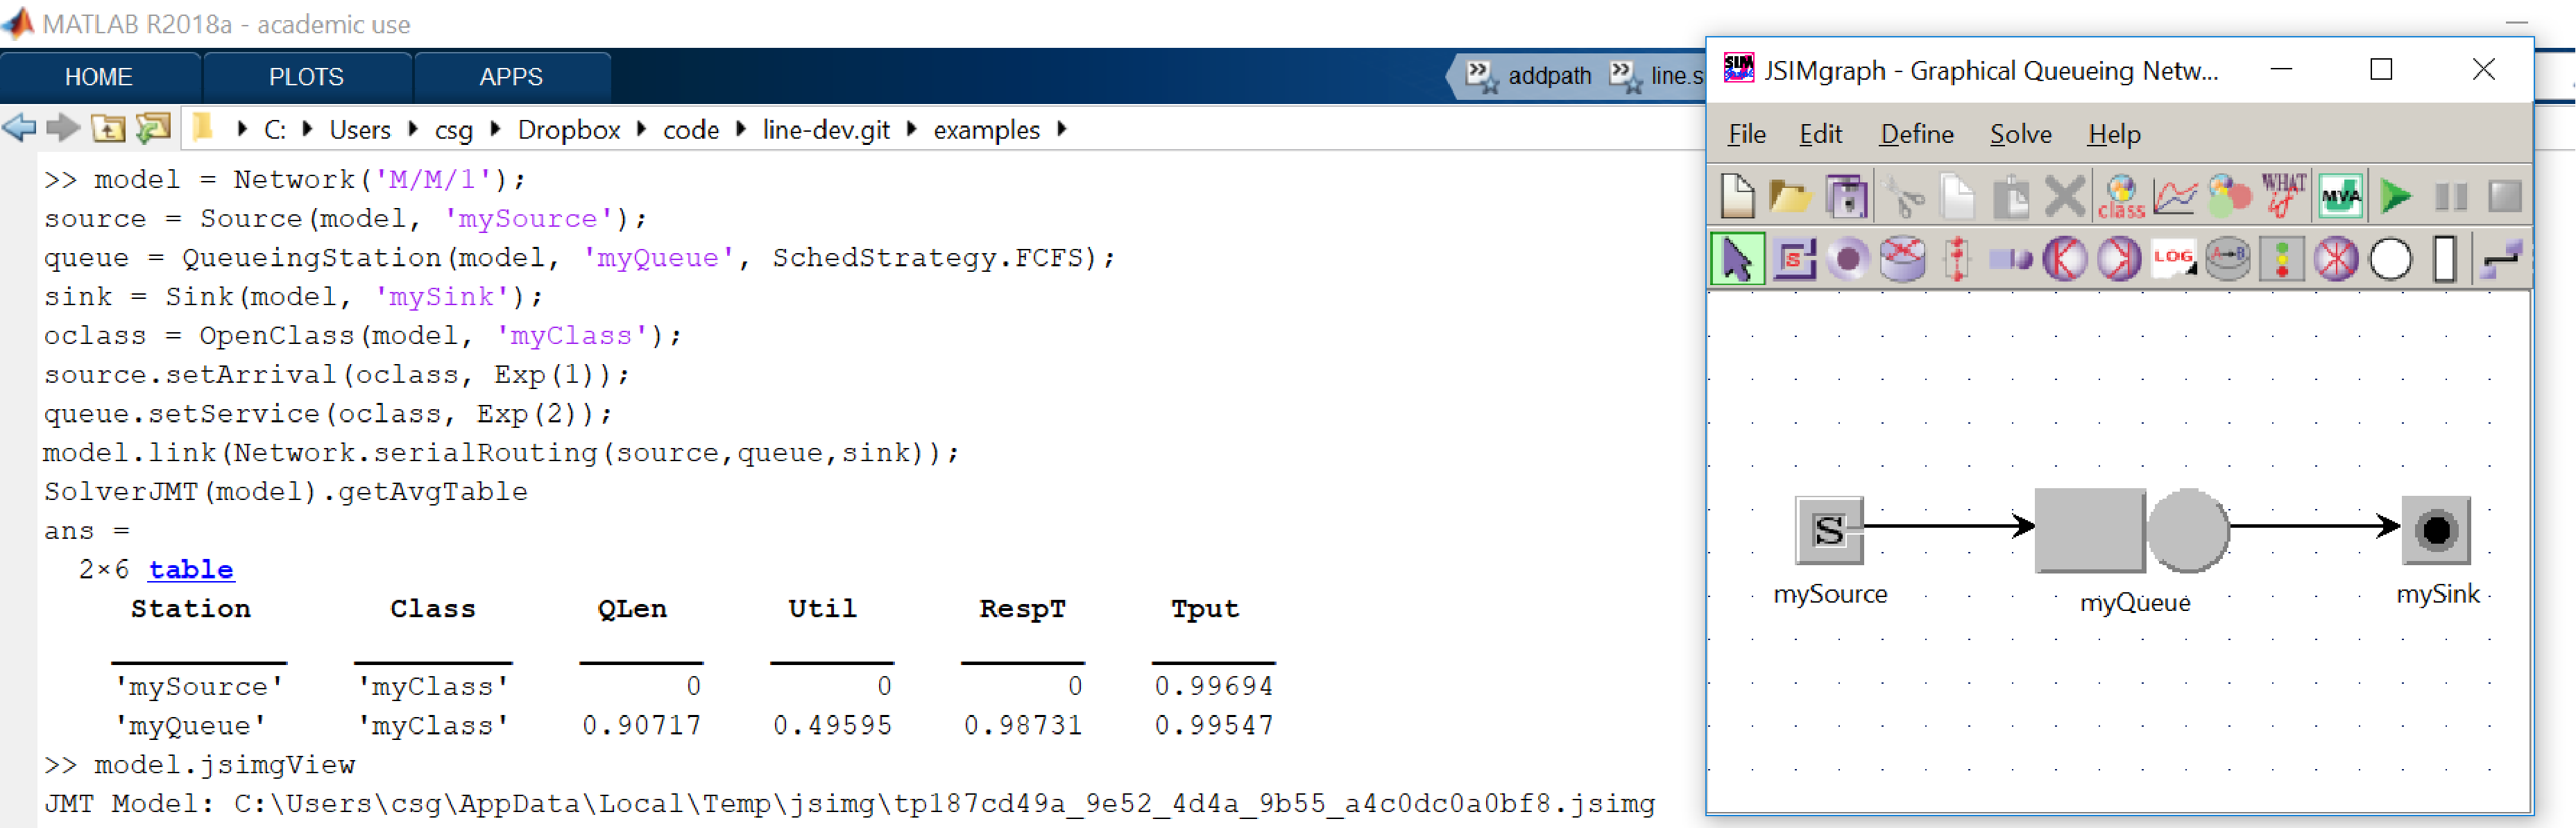
\includegraphics[width=14cm]{./images/jsimgViewMM1.pdf}
  \caption{M/M/1 example in JSIMgraph launched from MATLAB}\label{FIG:jsimgViewMM1}
\end{figure}
\end{MATLAB}
\begin{JAVA}
\begin{lstlisting}[language = java, basicstyle=\ttfamily\scriptsize]
model.jsimgView()
\end{lstlisting}
which will open the model inside JSIMgraph, as shown in Figure~\ref{FIG:jsimgViewMM1}. From this screen, the simulation can be started using the green ``play'' button in the JSIMgraph toolbar.
\begin{figure}[t!]
  \centering
  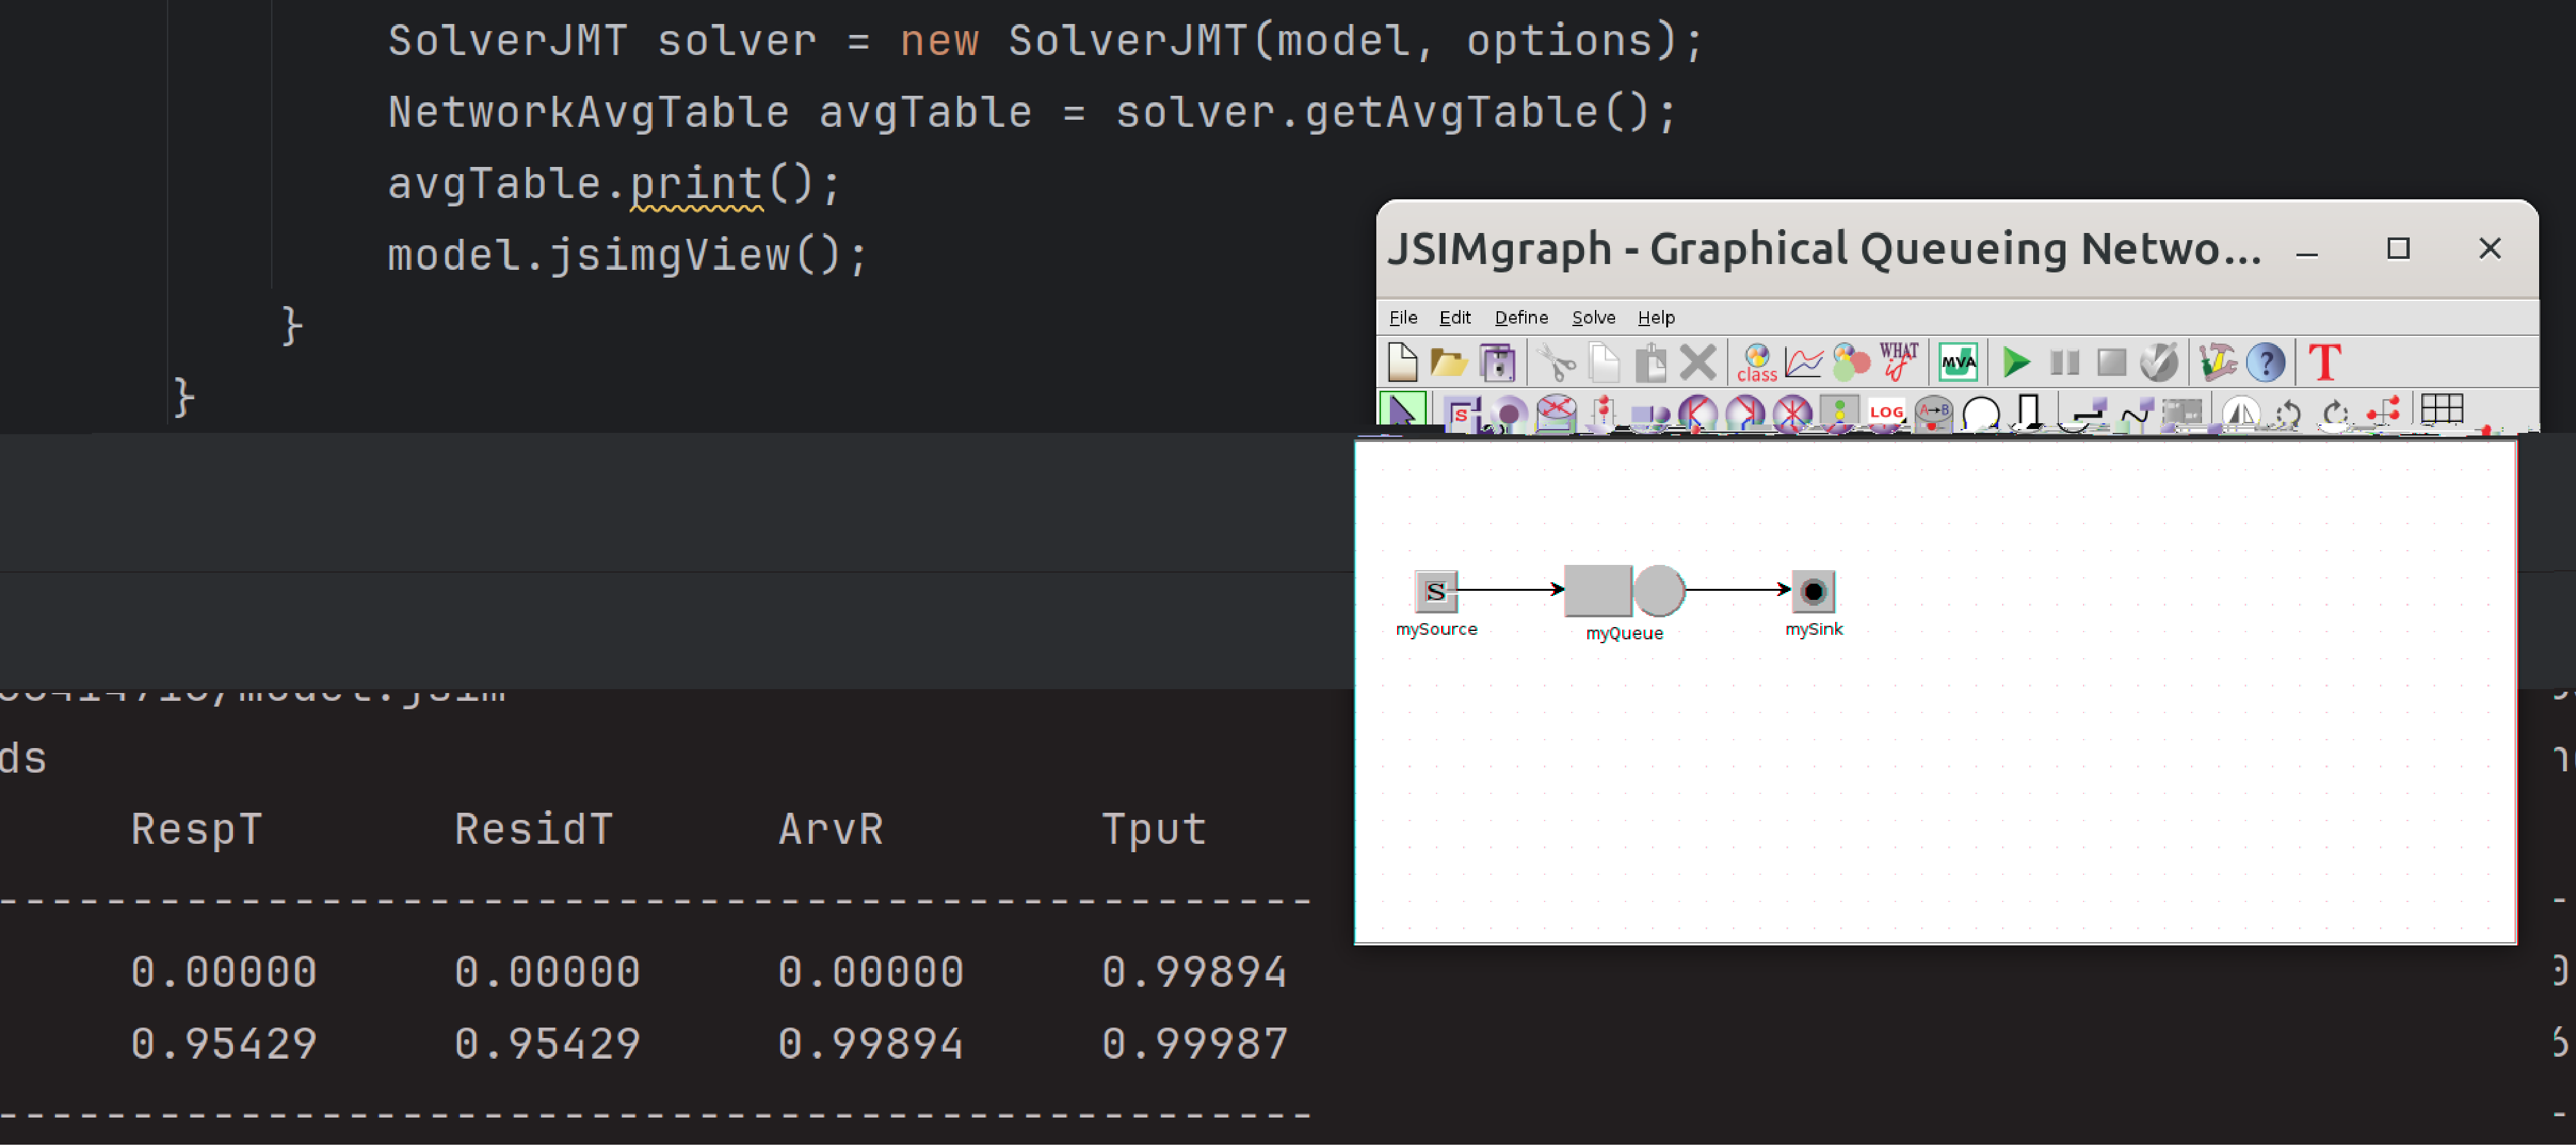
\includegraphics[width=13cm]{./images/jsimgViewMM1_Java.pdf}
  \caption{M/M/1 example in JSIMgraph}\label{FIG:jsimgViewMM1}
\end{figure}
\end{JAVA}
\begin{KOTLIN}
\begin{lstlisting}[language = kotlin, basicstyle=\ttfamily\scriptsize]
model.jsimgView()
\end{lstlisting}
which will open the model inside JSIMgraph, as shown in Figure~\ref{FIG:jsimgViewMM1}. From this screen, the simulation can be started using the green ``play'' button in the JSIMgraph toolbar.
\begin{figure}[t!]
  \centering
  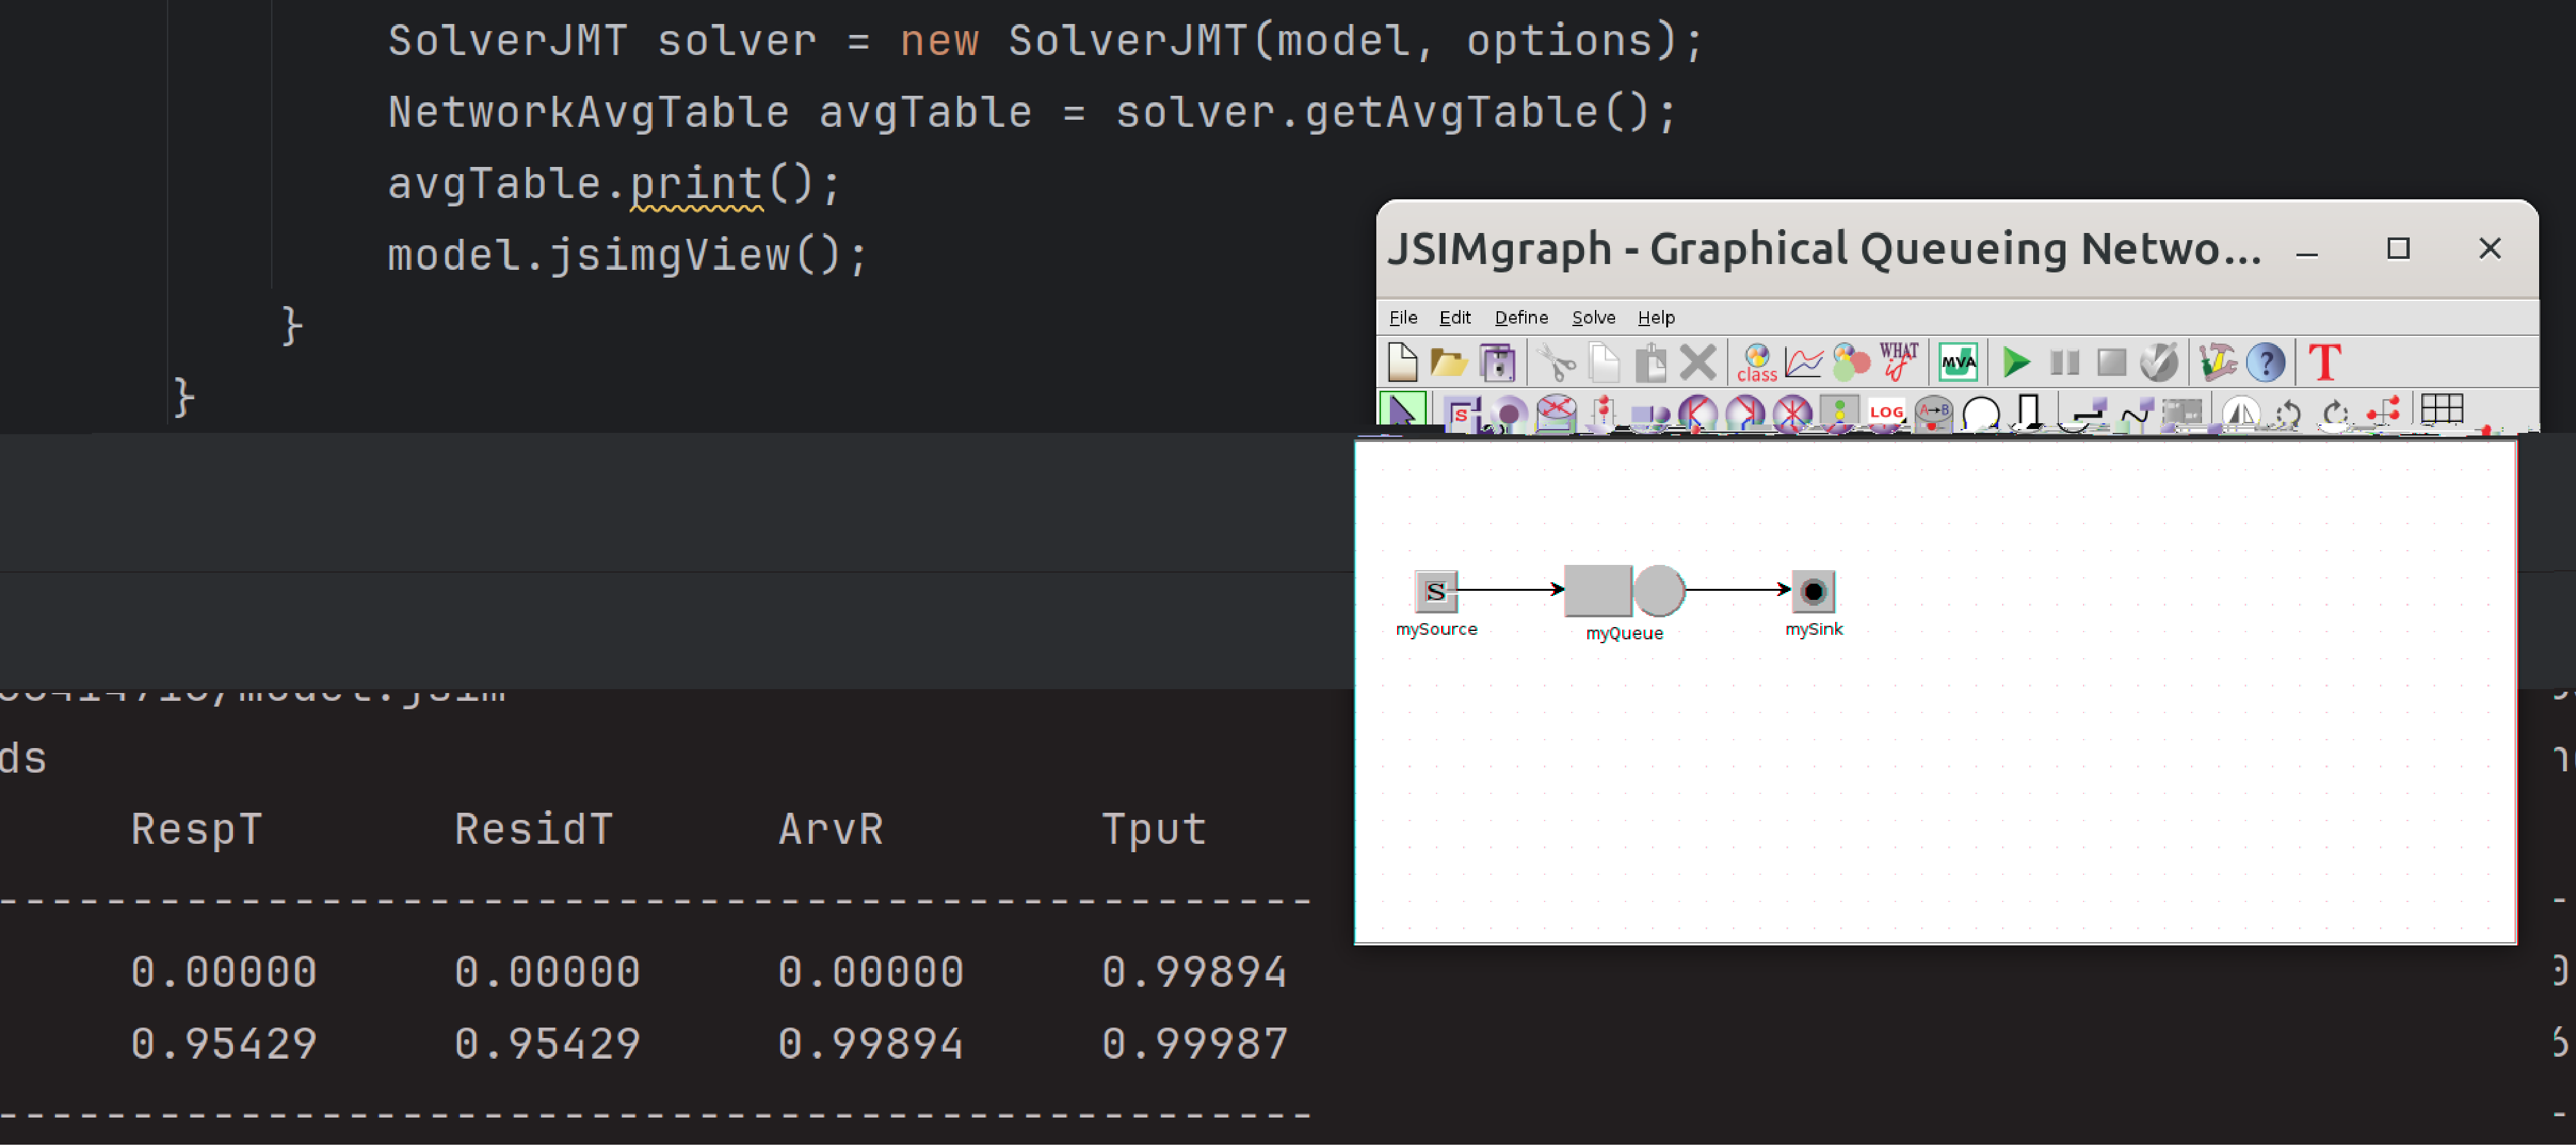
\includegraphics[width=13cm]{./images/jsimgViewMM1_Java.pdf}
  \caption{M/M/1 example in JSIMgraph}\label{FIG:jsimgViewMM1}
\end{figure}
\end{KOTLIN}
\begin{PYTHON}
\begin{lstlisting}[language = python]
model.jsimg_view()
\end{lstlisting}
which will open the model inside JSIMgraph, as shown in Figure~\ref{FIG:jsimgViewMM1}. From this screen, the simulation can be started using the green ``play'' button in the JSIMgraph toolbar.
\begin{figure}[t!]
  \centering
  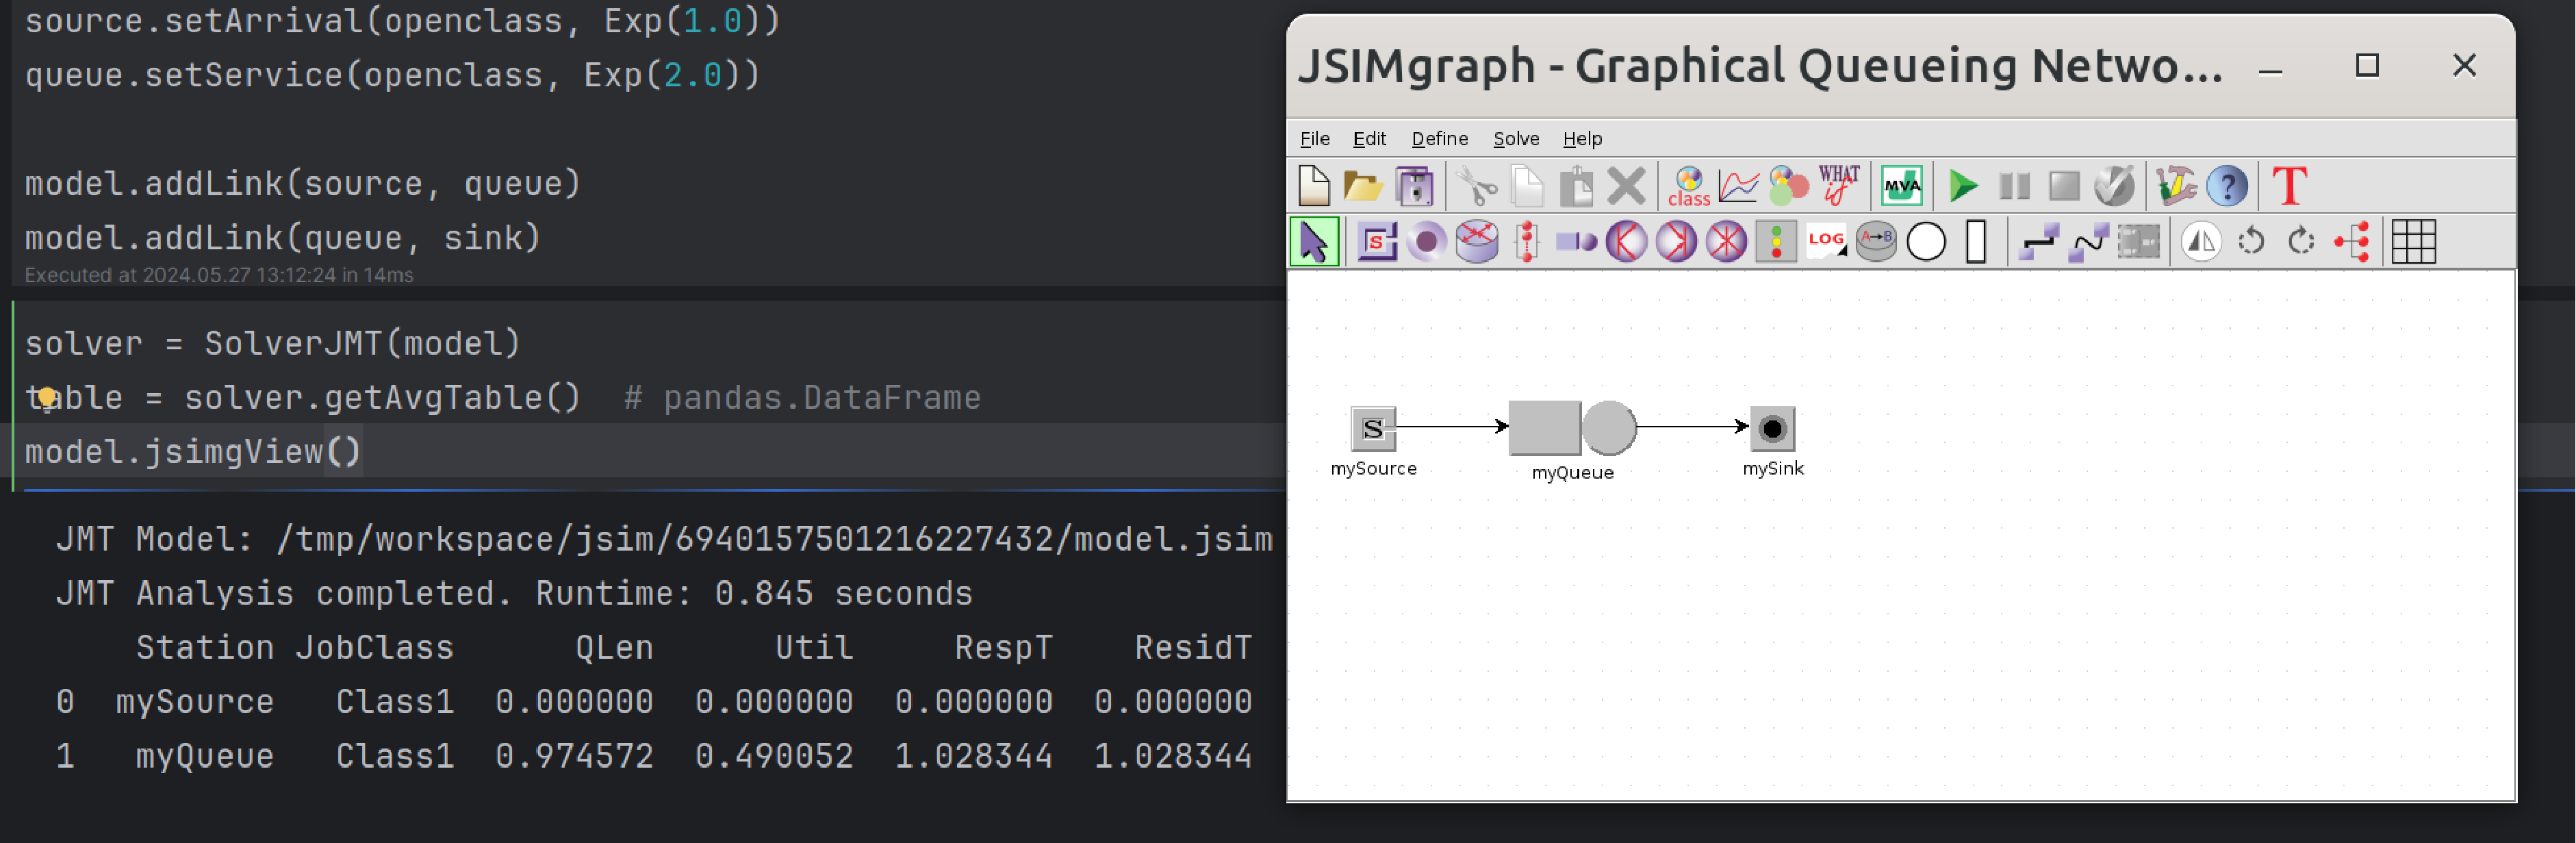
\includegraphics[width=13cm]{./images/jsimgViewMM1_Python.pdf}
  \caption{M/M/1 example in JSIMgraph}\label{FIG:jsimgViewMM1}
\end{figure}
\end{PYTHON}
%\textsc{Line} also offers shortcuts to accelerate the definition of basic models. For example, an M/M/1 with arrival rate $1$ and service rate $2$ can be readily instantiated as
%\begin{lstlisting}
%model = Network.tandemFcfs(1,2)
%\end{lstlisting}
A pre-defined gallery of classic models is also available, for example
\begin{MATLAB}
\begin{lstlisting}[language = matlab]
model = gallery_mm1
\end{lstlisting}    
\end{MATLAB}
\begin{JAVA}
\begin{lstlisting}[language = kotlin, basicstyle=\ttfamily\scriptsize]
Network model = gallery_mm1();
\end{lstlisting} 
\end{JAVA}
\begin{KOTLIN}
\begin{lstlisting}[language = kotlin, basicstyle=\ttfamily\scriptsize]
val model = gallery_mm1()
\end{lstlisting} 
\end{KOTLIN}
\begin{PYTHON}
\begin{lstlisting}[language = python]
model = gallery_mm1()
\end{lstlisting}    
\end{PYTHON}
returns a M/M/1 queue with $50\%$ utilization.

If we want to select a particular row of the \Matlab{\texttt{AvgTable}}\Java{\texttt{avgTable}}\Kotlin{\texttt{avgTable}}\Python{\texttt{avg\_table}} data structure, we can use direct object-based indexing or filtering methods. In \Matlab{}, we wrap the table with \texttt{IndexedAvgTable} to enable convenient syntax:
\begin{MATLAB}
\begin{lstlisting}[language = matlab]
>> AvgTable = IndexedAvgTable(AvgTable_native);
>> ARow = AvgTable(queue, jobclass)
ans =
  1x7 table
    Station    JobClass     QLen      Util       RespT     ResidT      Tput
    _______    ________    ______    _______    _______    _______    _______
    Queue      Class1      0.9555    0.48736    0.95429    0.95429    0.99987
\end{lstlisting}
For filtering by only station or class, use the \texttt{filterBy} method. If we specify only \texttt{queue} or \texttt{jobclass}, \texttt{filterBy} will return all entries corresponding to that station or class.
\end{MATLAB}
\begin{JAVA}
\begin{lstlisting}[language = java, basicstyle=\ttfamily\scriptsize]
avgTable.tget("Queue", "Class1").print();
\end{lstlisting}
gives output
\begin{lstlisting}[language = java, basicstyle=\ttfamily\scriptsize]
Station   	JobClass  	QLen      	Util      	RespT     	ResidT    	ArvR      	Tput      
-------------------------------------------------------------------------------------------
Queue   	Class1   	0.95550   	0.48736   	0.95429   	0.95429   	0.99894   	0.99987   
--------------------------------------------------------------------------------------------
\end{lstlisting}
If we specify only \texttt{"Queue"} or \texttt{"Class1"}, \texttt{tget} will return all entries corresponding to that station or class.
\end{JAVA}
\begin{KOTLIN}
\begin{lstlisting}[language = kotlin, basicstyle=\ttfamily\scriptsize]
avgTable.tget("Queue", "Class1").print()
\end{lstlisting}
gives output
\begin{lstlisting}[language = kotlin, basicstyle=\ttfamily\scriptsize]
Station   	JobClass  	QLen      	Util      	RespT     	ResidT    	ArvR      	Tput      
-------------------------------------------------------------------------------------------
Queue   	Class1   	0.95550   	0.48736   	0.95429   	0.95429   	0.99894   	0.99987   
--------------------------------------------------------------------------------------------
\end{lstlisting}
If we specify only \texttt{"Queue"} or \texttt{"Class1"}, \texttt{tget} will return all entries corresponding to that station or class.
\end{KOTLIN}
\begin{PYTHON}
\begin{lstlisting}[language = python]
ARow = tget(avg_table, 'Queue', 'Class1')
\end{lstlisting}
gives output
\begin{lstlisting}[language = python]
   Station JobClass      QLen     Util     RespT    ResidT      Tput
1  Queue  Class1  0.955501  0.48736  0.954293  0.954293  0.999868
\end{lstlisting}
If we specify only \texttt{'Queue'} or \texttt{'Class1'}, \texttt{tget} will return all entries corresponding to that station or class.
\end{PYTHON}
The same indexing works with Station and JobClass objects:
\begin{MATLAB}
\begin{lstlisting}[language = matlab]
>> ARow = AvgTable(queue, jobclass)
\end{lstlisting}
\end{MATLAB}
\begin{JAVA}
\begin{lstlisting}[language = java, basicstyle=\ttfamily\scriptsize]
avgTable.tget(queue, jobclass).print();
\end{lstlisting}
\end{JAVA}
\begin{KOTLIN}
\begin{lstlisting}[language = kotlin, basicstyle=\ttfamily\scriptsize]
avgTable.tget(queue, jobclass).print()
\end{lstlisting}
\end{KOTLIN}
\begin{PYTHON}
\begin{lstlisting}[language = python]
ARow = tget(AvgTable, queue, jobclass)
\end{lstlisting}
\end{PYTHON}
if we specify only \texttt{queue} or only \texttt{jobclass}, \Matlab{tget} will return all entries corresponding to that station or class.


\subsection{Tutorial 2: A multiclass M/G/1 queue}
\label{example-2-multiclass-mgk-queue}
We now consider a more challenging variant of the first example. We assume that there are two classes of incoming jobs with non-exponential service times. For the first class, service times are Erlang distributed with unit rate and variance $1/3$; they are instead read from a trace for the second class. Both classes have exponentially distributed inter-arrival times with mean $2s$.

To run this example, let us first change the working directory to the \texttt{examples/} folder. Then we specify the node block
\begin{MATLAB}
\begin{lstlisting}[language = matlab]
model = Network('M/G/1');
source = Source(model,'Source');
queue = Queue(model, 'Queue', SchedStrategy.FCFS);
sink = Sink(model,'Sink');
\end{lstlisting}
\end{MATLAB}
\begin{JAVA}
\begin{lstlisting}[language = java, basicstyle=\ttfamily\scriptsize]
Network model = new Network("M/G/1");
Source source = new Source(model, "Source");
Queue queue = new Queue(model, "Queue", SchedStrategy.FCFS);
Sink sink = new Sink(model, "Sink");
\end{lstlisting}
\end{JAVA}
\begin{KOTLIN}
\begin{lstlisting}[language = kotlin, basicstyle=\ttfamily\scriptsize]
val model = Network("M/G/1")
val source = Source(model, "Source")
val queue = Queue(model, "Queue", SchedStrategy.FCFS)
val sink = Sink(model, "Sink")
\end{lstlisting}
\end{KOTLIN}
\begin{PYTHON}
\begin{lstlisting}[language = python]
model = Network('M/G/1')
source = Source(model,'Source')
queue = Queue(model, 'Queue', SchedStrategy.FCFS)
sink = Sink(model,'Sink')
\end{lstlisting}
\end{PYTHON}
The next step consists in defining the classes. We fit automatically from mean and squared coefficient of variation (i.e.,  SCV=variance/mean$^2$) an Erlang distribution and use the \texttt{Replayer} distribution to request that the specified trace is read cyclically to obtain the service times of class 2
\begin{MATLAB}
\begin{lstlisting}[language = matlab]
jobclass1 = OpenClass(model, 'Class1');
jobclass2 = OpenClass(model, 'Class2');

source.setArrival(jobclass1, Exp(0.5));
source.setArrival(jobclass2, Exp(0.5));

queue.setService(jobclass1, Erlang.fitMeanAndSCV(1, 1/3));
queue.setService(jobclass2, Replayer('example_trace.txt'));
\end{lstlisting}
\end{MATLAB}
\begin{JAVA}
\begin{lstlisting}[language = java, basicstyle=\ttfamily\scriptsize]
OpenClass jobclass1 = new OpenClass(model, "Class1");
OpenClass jobclass2 = new OpenClass(model, "Class2");
source.setArrival(jobclass1, new Exp(0.5));
source.setArrival(jobclass2, new Exp(0.5));
queue.setService(jobclass1, Erlang.fitMeanAndSCV(1, (double) 1 / 3));
try {
URI fileURI = GettingStarted.class.getResource("/example_trace.txt").toURI();
String fileName = Paths.get(fileURI).toString();
    queue.setService(jobclass2, new Replayer(fileName));
} catch (URISyntaxException e) {
    throw new RuntimeException(e);
}
\end{lstlisting}
\end{JAVA}
\begin{KOTLIN}
\begin{lstlisting}[language = kotlin, basicstyle=\ttfamily\scriptsize]
val jobclass1 = OpenClass(model, "Class1", 0)
val jobclass2 = OpenClass(model, "Class2", 0)
source.setArrival(jobclass1, Exp(0.5))
source.setArrival(jobclass2, Exp(0.5))
queue.setService(jobclass1, Erlang.fitMeanAndSCV(1.0, 1.0 / 3.0))
try {
    val fileURI = GettingStarted::class.java.getResource("/example_trace.txt")!!.toURI()
    val fileName = Paths.get(fileURI).toString()
    queue.setService(jobclass2, Replayer(fileName))
} catch (e: URISyntaxException) {
    throw RuntimeException(e)
}
\end{lstlisting}
\end{KOTLIN}
\begin{PYTHON}
\begin{lstlisting}[language = python]
jobclass1 = OpenClass(model, 'Class1')
jobclass2 = OpenClass(model, 'Class2')

source.set_arrival(jobclass1, Exp(0.5))
source.set_arrival(jobclass2, Exp(0.5))

queue.set_service(jobclass1, Erlang.fit_mean_and_scv(1, 1/3))
queue.set_service(jobclass2, Replayer('example_trace.txt'))
\end{lstlisting}
\end{PYTHON}
Note that the \texttt{example\_trace.txt} file consists of a single column of doubles, each representing a service time value, e.g.,
\begin{lstlisting}[basicstyle=\ttfamily\scriptsize]
   1.2377474e-02
   4.4486055e-02
   1.0027642e-02
   2.0983173e-02
   ...
\end{lstlisting}
We now specify a linear route through source, queue, and sink for both classes
\begin{MATLAB}
\begin{lstlisting}[language = matlab]
P = model.initRoutingMatrix();
P{jobclass1} = Network.serialRouting(source,queue,sink);
P{jobclass2} = Network.serialRouting(source,queue,sink);
model.link(P);
\end{lstlisting}
\end{MATLAB}
\begin{JAVA}
\begin{lstlisting}[language = java, basicstyle=\ttfamily\scriptsize]
Matrix P = model.initRoutingMatrix();
P.set(jobclass1, jobclass1, Network.serialRouting(source,queue,sink));
P.set(jobclass2, jobclass2, Network.serialRouting(source,queue,sink));
model.link(P);
\end{lstlisting}
\end{JAVA}
\begin{KOTLIN}
\begin{lstlisting}[language = kotlin, basicstyle=\ttfamily\scriptsize]
val P = model.initRoutingMatrix()
P.set(jobclass1, jobclass1, Network.serialRouting(source, queue, sink))
P.set(jobclass2, jobclass2, Network.serialRouting(source, queue, sink))
model.link(P)
\end{lstlisting}
\end{KOTLIN}
\begin{PYTHON}
\begin{lstlisting}[language = python]
P = model.init_routing_matrix()
P.set(jobclass1,Network.serial_routing(source,queue,sink))
P.set(jobclass2,Network.serial_routing(source,queue,sink))
model.link(P)
\end{lstlisting}
\end{PYTHON}
and solve the model with JMT
\begin{MATLAB}
\begin{lstlisting}[language = matlab]
>>jmtAvgTable = JMT(model,'seed',23000).avgTable()
jmtAvgTable =
  4x7 table
    Station    JobClass     QLen        Util       RespT     ResidT      Tput
    _______    ________    _______    ________    _______    _______    _______
    Source      Class1           0           0          0          0    0.50017
    Source      Class2           0           0          0          0    0.49114
    Queue       Class1     0.86153      0.4984     1.7389     1.7389    0.49953
    Queue       Class2     0.43751    0.049184    0.85879    0.85879    0.49064
\end{lstlisting}
\end{MATLAB}
\begin{JAVA}
\begin{lstlisting}[language = java, basicstyle=\ttfamily\scriptsize]
NetworkAvgTable avgTable = new JMT(model).avgTable();
avgTable.print();
\end{lstlisting}
which gives
\begin{lstlisting}[basicstyle=\ttfamily\scriptsize]
Station   	JobClass  	QLen      	Util      	RespT     	ResidT    	ArvR      	Tput      
--------------------------------------------------------------------------------------------
Source    	Class1    	0          	0          	0          	0          	0          	0.50017   
Source    	Class2    	0          	0          	0          	0          	0          	0.49114   
Queue     	Class1    	0.86153   	0.49840   	1.73889   	1.73889   	0.50017   	0.49953   
Queue     	Class2    	0.43751   	0.04918   	0.85879   	0.85879   	0.49114   	0.49064   
--------------------------------------------------------------------------------------------
\end{lstlisting}
\end{JAVA}
\begin{KOTLIN}
\begin{lstlisting}[language = kotlin, basicstyle=\ttfamily\scriptsize]
val avgTable: NetworkAvgTable = JMT(model).avgTable()
avgTable.print()
\end{lstlisting}
which gives
\begin{lstlisting}[basicstyle=\ttfamily\scriptsize]
Station   	JobClass  	QLen      	Util      	RespT     	ResidT    	ArvR      	Tput      
--------------------------------------------------------------------------------------------
Source    	Class1    	0          	0          	0          	0          	0          	0.50017   
Source    	Class2    	0          	0          	0          	0          	0          	0.49114   
Queue     	Class1    	0.86153   	0.49840   	1.73889   	1.73889   	0.50017   	0.49953   
Queue     	Class2    	0.43751   	0.04918   	0.85879   	0.85879   	0.49114   	0.49064   
--------------------------------------------------------------------------------------------
\end{lstlisting}
\end{KOTLIN}
\begin{PYTHON}
\begin{lstlisting}[language = python]
jmt_avg_table = JMT(model, seed=23000).avg_table()
print(jmt_avg_table)
\end{lstlisting}
which gives
\begin{lstlisting}[basicstyle=\ttfamily\scriptsize]
JMT Model: /tmp/workspace/jsim/7955719514502154869/model.jsim
JMT Analysis completed. Runtime: 1.06 seconds
  Station JobClass      QLen      Util     RespT    ResidT      Tput
0  Source   Class1  0         0         0         0         0.501685
1  Source   Class2  0         0         0         0         0.506538
2   Queue   Class1  0.880661  0.494749  1.737321  1.737321  0.506679
3   Queue   Class2  0.438433  0.053432  0.817414  0.817414  0.507503
\end{lstlisting}
\end{PYTHON}
We wish now to validate this value against an analytical solver. Since \texttt{jobclass2} has trace-based service times, we first need to revise its service time distribution to make it analytically tractable, e.g., we may ask \textsc{Line} to fit an acyclic phase-type distribution~\cite{BobHST03} based on the trace
\begin{MATLAB}
\begin{lstlisting}[language = matlab]
queue.setService(jobclass2, Replayer('example_trace.txt').fitAPH());
\end{lstlisting}
\end{MATLAB}
\begin{JAVA}
\begin{lstlisting}[language = java, basicstyle=\ttfamily\scriptsize]
queue.setService(jobclass2, new Replayer(fileName).fitAPH());
\end{lstlisting}
\end{JAVA}
\begin{KOTLIN}
\begin{lstlisting}[language = kotlin, basicstyle=\ttfamily\scriptsize]
queue.setService(jobclass2, Replayer(fileName).fitAPH())
\end{lstlisting}
\end{KOTLIN}
\begin{PYTHON}
\begin{lstlisting}[language = python]
queue.set_service(jobclass2, Replayer('example_trace.txt').fit_aph())
\end{lstlisting}
\end{PYTHON}
We can now use a Continuous Time Markov Chain (CTMC) to solve the system, but since the state space is infinite in open models, we need to truncate it to be able to use this solver. For example, we may restrict to states with at most 2 jobs in each class, checking with the \texttt{verbose} option the size of the resulting state space
\begin{MATLAB}
\begin{lstlisting}[language = matlab]
>> ctmcAvgTable2 = CTMC(model,'cutoff',2,'verbose',true).avgTable()
State space size: 46 states.
CTMC analysis completed in 0.096734 sec
ctmcAvgTable2 =
  4x7 table
    Station    JobClass     QLen        Util       RespT     ResidT      Tput
    _______    ________    _______    ________    _______    _______    _______
    Source      Class1           0           0          0          0    0.44948
    Source      Class2           0           0          0          0    0.48424
    Queue       Class1     0.56734     0.44948     1.2863     1.2863    0.44107
    Queue       Class2     0.24456    0.048942    0.51396    0.51396    0.47583
\end{lstlisting}
\end{MATLAB}
\begin{JAVA}
\begin{lstlisting}[language = java, basicstyle=\ttfamily\scriptsize]
new CTMC(model,"cutoff",2,"verbose", VerboseLevel.STD).avgTable().print();
Station  JobClass  QLen        Util        RespT       ResidT      ArvR        Tput        
-------------------------------------------------------------------------------------------
Source   Class1    0           0           0           0           0           0.44108     
Source   Class2    0           0           0           0           0           0.47594     
Queue    Class1    0.56714     0.44108     1.28578     1.28578     0.44108     0.44108     
Queue    Class2    0.24423     0.04810     0.51316     0.51316     0.47594     0.47594     
-------------------------------------------------------------------------------------------
\end{lstlisting}
\end{JAVA}
\begin{KOTLIN}
\begin{lstlisting}[language = kotlin, basicstyle=\ttfamily\scriptsize]
CTMC(model,"cutoff",2,"verbose", VerboseLevel.STD).avgTable().print()
Station  JobClass  QLen        Util        RespT       ResidT      ArvR        Tput        
-------------------------------------------------------------------------------------------
Source   Class1    0           0           0           0           0           0.44108     
Source   Class2    0           0           0           0           0           0.47594     
Queue    Class1    0.56714     0.44108     1.28578     1.28578     0.44108     0.44108     
Queue    Class2    0.24423     0.04810     0.51316     0.51316     0.47594     0.47594     
-------------------------------------------------------------------------------------------
\end{lstlisting}
\end{KOTLIN}
\begin{PYTHON}
\begin{lstlisting}[language = python]
ctmc_avg_table2 = CTMC(model, cutoff=2, verbose=True).avg_table()
print(ctmc_avg_table2)
\end{lstlisting}
which gives
\begin{lstlisting}[basicstyle=\ttfamily\scriptsize]
  Station JobClass    QLen    Util   RespT  ResidT    ArvR    Tput
0  Source   Class1  0.0000  0.0000  0.0000  0.0000  0.0000  0.4411
1  Source   Class2  0.0000  0.0000  0.0000  0.0000  0.0000  0.4758
2   Queue   Class1  0.5674  0.4411  1.2863  1.2863  0.4411  0.4411
3   Queue   Class2  0.2446  0.0481  0.5140  0.5140  0.4758  0.4758
\end{lstlisting}
\end{PYTHON}
However, we see from the comparison with JMT that the errors of \texttt{CTMC} are rather large. Since the truncated state space consists of just 46 states, we can further increase the cutoff to 4, trading a slower solution time for higher precision
\begin{MATLAB}
\begin{lstlisting}[language = matlab]
>> ctmcAvgTable4 = CTMC(model,'cutoff',4,'verbose',true).avgTable()
State space size: 626 states.
CTMC analysis completed in 1.051784 sec
ctmcAvgTable4 =
  4x7 table
    Station    JobClass     QLen        Util       RespT     ResidT      Tput
    _______    ________    _______    ________    _______    _______    _______
    Source      Class1           0           0          0          0    0.49215
    Source      Class2           0           0          0          0    0.49626
    Queue       Class1      0.7958     0.49215     1.6187     1.6187    0.49162
    Queue       Class2     0.37558    0.050157    0.75763    0.75763    0.49573
\end{lstlisting}
\end{MATLAB}
\begin{JAVA}
\begin{lstlisting}[language = java, basicstyle=\ttfamily\scriptsize]
new CTMC(model,"cutoff",4).avgTable().print();
\end{lstlisting}
which gives
\begin{lstlisting}[basicstyle=\ttfamily\scriptsize]
-------------------------------------------------------------------------------------------
Station  JobClass  QLen        Util        RespT       ResidT      ArvR        Tput        
-------------------------------------------------------------------------------------------
Source   Class1    0           0           0           0           0           0.49160     
Source   Class2    0           0           0           0           0           0.49570     
Queue    Class1    0.79557     0.49160     1.61832     1.61832     0.49160     0.49160     
Queue    Class2    0.37532     0.05010     0.75716     0.75716     0.49570     0.49570     
-------------------------------------------------------------------------------------------
\end{lstlisting}
\end{JAVA}
\begin{KOTLIN}
\begin{lstlisting}[language = kotlin, basicstyle=\ttfamily\scriptsize]
CTMC(model,"cutoff",4).avgTable().print()
\end{lstlisting}
which gives
\begin{lstlisting}[basicstyle=\ttfamily\scriptsize]
-------------------------------------------------------------------------------------------
Station  JobClass  QLen        Util        RespT       ResidT      ArvR        Tput        
-------------------------------------------------------------------------------------------
Source   Class1    0           0           0           0           0           0.49160     
Source   Class2    0           0           0           0           0           0.49570     
Queue    Class1    0.79557     0.49160     1.61832     1.61832     0.49160     0.49160     
Queue    Class2    0.37532     0.05010     0.75716     0.75716     0.49570     0.49570     
-------------------------------------------------------------------------------------------
\end{lstlisting}
\end{KOTLIN}
\begin{PYTHON}
\begin{lstlisting}[language = python]
ctmc_avg_table4 = CTMC(model, cutoff=4, verbose=True).avg_table()
print(ctmc_avg_table4)
\end{lstlisting}
which gives
\begin{lstlisting}[basicstyle=\ttfamily\scriptsize]
  Station JobClass    QLen    Util   RespT  ResidT    ArvR    Tput
0  Source   Class1  0.0000  0.0000  0.0000  0.0000  0.0000  0.4916
1  Source   Class2  0.0000  0.0000  0.0000  0.0000  0.0000  0.4957
2   Queue   Class1  0.7958  0.4916  1.6188  1.6188  0.4916  0.4916
3   Queue   Class2  0.3756  0.0501  0.7577  0.7577  0.4957  0.4957
\end{lstlisting}
\end{PYTHON}
To gain more accuracy, we could either keep increasing the cutoff value or, if we wish to compute an exact solution, we may call the matrix-analytic method (MAM) solver instead. \texttt{MAM} uses the repetitive structure of the CTMC to exactly analyze open systems with an infinite state space, calling
\begin{MATLAB}
\begin{lstlisting}[language = matlab]
>> mamAvgTable = MAM(model).avgTable()
mamAvgTable =
  4x7 table
    Station    JobClass     QLen        Util       RespT     ResidT     Tput
    _______    ________    _______    ________    _______    _______    ____
    Source      Class1           0           0          0          0    0.5
    Source      Class2           0           0          0          0    0.5
    Queue       Class1     0.87646         0.5     1.7529     1.7529    0.5
    Queue       Class2       0.427    0.050536    0.85399    0.85399    0.5
\end{lstlisting}
The current \texttt{MAM} implementation is primarily constructed on top of the BuTools solver~\cite{Hor17}, the SMC solver~\cite{BiniMSPH12}, and MAMSolver (\url{https://www.cs.wm.edu/MAMSolver/}).
\end{MATLAB}
\begin{JAVA}
\begin{lstlisting}[language = java, basicstyle=\ttfamily\scriptsize]
new MAM(model).avgTable().print();
\end{lstlisting}
we get
\begin{lstlisting}[language = java, basicstyle=\ttfamily\scriptsize]
Station   	JobClass  	QLen      	Util      	RespT     	ResidT    	ArvR      	Tput      
--------------------------------------------------------------------------------------------
Source    	Class1    	0         	0         	0         	0         	0         	0.50000   
Source    	Class2    	0         	0         	0         	0         	0         	0.50000   
Queue     	Class1    	0.87649   	0.50000   	1.75299   	1.75299   	0.50000   	0.50000   
Queue     	Class2    	0.42703   	0.05054   	0.85406   	0.85406   	0.50000   	0.50000   
--------------------------------------------------------------------------------------------
\end{lstlisting}
\end{JAVA}
\begin{KOTLIN}
\begin{lstlisting}[language = kotlin, basicstyle=\ttfamily\scriptsize]
MAM(model).avgTable().print()
\end{lstlisting}
we get
\begin{lstlisting}[language = kotlin, basicstyle=\ttfamily\scriptsize]
Station   	JobClass  	QLen      	Util      	RespT     	ResidT    	ArvR      	Tput      
--------------------------------------------------------------------------------------------
Source    	Class1    	0         	0         	0         	0         	0         	0.50000   
Source    	Class2    	0         	0         	0         	0         	0         	0.50000   
Queue     	Class1    	0.87649   	0.50000   	1.75299   	1.75299   	0.50000   	0.50000   
Queue     	Class2    	0.42703   	0.05054   	0.85406   	0.85406   	0.50000   	0.50000   
--------------------------------------------------------------------------------------------
\end{lstlisting}
\end{KOTLIN}
\begin{PYTHON}
\begin{lstlisting}[language = python]
print(MAM(model).avg_table())
\end{lstlisting}
we get
\begin{lstlisting}[basicstyle=\ttfamily\scriptsize]
  Station JobClass      QLen      Util     RespT    ResidT  ArvR  Tput
0  Source   Class1  0         0         0         0          0.5   0.5
1  Source   Class2  0         0         0         0          0.5   0.5
2   Queue   Class1  0.876460  0.500000  1.752920  1.752920   0.5   0.5
3   Queue   Class2  0.426996  0.050536  0.853991  0.853991   0.5   0.5
\end{lstlisting}
The current \texttt{MAM} implementation is primarily constructed on top of Java ports of the BuTools solver~\cite{Hor17} and the SMC solver~\cite{BiniMSPH12}.
\end{PYTHON}

\subsection{Tutorial 3: Machine interference problem}
\label{example-3-machine-interference-problem}
Closed models involve jobs that perpetually cycle within a network of queues. The machine interference problem is a classic example, in which a group of repairmen is tasked with fixing machines as they break and the goal is to choose the optimal size of the group. We here illustrate how to evaluate the performance of a given group size. We consider a scenario with $S=2$ repairmen, with machines that break down at a rate of $0.5$ failed machines/week, after which a machine is fixed in an exponential distributed time with rate $4.0$ repaired machines/week. There are a total of $N=3$ machines.

Suppose that we wish to obtain an exact numerical solution using Continuous Time Markov Chains (CTMCs). The above model can be analyzed as follows:
\begin{MATLAB}
\begin{lstlisting}[language = matlab]
model = Network('MRP');
%% Block 1: nodes
delay = Delay(model,'WorkingState');
queue = Queue(model, 'RepairQueue', SchedStrategy.FCFS);
queue.setNumberOfServers(S);
%% Block 2: classes
cclass = ClosedClass(model, 'Machines', N, delay);
delay.setService(cclass, Exp(0.5));
queue.setService(cclass, Exp(4.0));
%% Block 3: topology
model.link(Network.serialRouting(delay,queue));
%% Block 4: solution
solver = CTMC(model);
ctmcAvgTable = solver.avgTable()
\end{lstlisting}
\end{MATLAB}
\begin{JAVA}
\begin{lstlisting}[language = java, basicstyle=\ttfamily\scriptsize]
Network model = new Network("MRP");
Delay delay = new Delay(model, "WorkingState");
Queue queue = new Queue(model, "RepairQueue", SchedStrategy.FCFS);
queue.setNumberOfServers(2);

ClosedClass closedClass = new ClosedClass(model, "Machines", 3, delay);
delay.setService(closedClass, new Exp(0.5));
queue.setService(closedClass, new Exp(4.0));
model.link(Network.serialRouting(delay, queue));
CTMC solver = new CTMC(model);
NetworkAvgTable ctmcAvgTable = solver.avgTable();
ctmcAvgTable.print();
\end{lstlisting}
\end{JAVA}
\begin{KOTLIN}
\begin{lstlisting}[language = kotlin, basicstyle=\ttfamily\scriptsize]
val model = Network("MRP")
val delay = Delay(model, "WorkingState")
val queue = Queue(model, "RepairQueue", SchedStrategy.FCFS)
queue.setNumberOfServers(2)

val closedClass = ClosedClass(model, "Machines", 3, delay)
delay.setService(closedClass, Exp(0.5))
queue.setService(closedClass, Exp(4.0))
model.link(Network.serialRouting(delay, queue))
val solver = CTMC(model)
val ctmcAvgTable = solver.avgTable()
ctmcAvgTable.print()
\end{lstlisting}
\end{KOTLIN}
\begin{PYTHON}
\begin{lstlisting}[language = python]
model = Network('MRP')
delay = Delay(model, 'WorkingState')
queue = Queue(model, 'RepairQueue', SchedStrategy.FCFS)
queue.set_number_of_servers(2)
cclass = ClosedClass(model, 'Machines', 3, delay)
delay.set_service(cclass, Exp(0.5))
queue.set_service(cclass, Exp(4.0))
model.link(Network.serialRouting(delay, queue))
solver = CTMC(model)
ctmc_avg_table = solver.avg_table()
print(ctmc_avg_table)
\end{lstlisting}
\end{PYTHON}
Here, \texttt{delay} appears in the constructor of the closed class to specify that a job will be considered completed once it returns to the delay (i.e., the machine returns in working state). We say that the delay is thus the \emph{reference station} of \texttt{cclass}. The above code prints the following result
\begin{MATLAB}
\begin{lstlisting}[language = matlab]
ctmcAvgTable =
  2x7 table
      Station       JobClass     QLen       Util       RespT     ResidT      Tput
    ____________    ________    _______    _______    _______    _______    ______
    WorkingState    Machines     2.6648     2.6648          2          2    1.3324
    RepairQueue     Machines    0.33516    0.16655    0.25154    0.25154    1.3324
\end{lstlisting}
\end{MATLAB}
\begin{JAVA}
\begin{lstlisting}[language = java, basicstyle=\ttfamily\scriptsize]
Station      JobClass   QLen     Util     RespT     ResidT    	ArvR        Tput   
--------------------------------------------------------------------------------------
WorkingState Machines  	2.66484  2.66484  2.00000  	2.00000   	0          	1.33242   
RepairQueue	 Machines  	0.33516  0.16655  0.25154  	0.25154   	0          	1.33242   
--------------------------------------------------------------------------------------
\end{lstlisting}
\end{JAVA}
\begin{KOTLIN}
\begin{lstlisting}[language = kotlin, basicstyle=\ttfamily\scriptsize]
Station      JobClass   QLen     Util     RespT     ResidT    	ArvR        Tput   
--------------------------------------------------------------------------------------
WorkingState Machines  	2.66484  2.66484  2.00000  	2.00000   	0          	1.33242   
RepairQueue	 Machines  	0.33516  0.16655  0.25154  	0.25154   	0          	1.33242   
--------------------------------------------------------------------------------------
\end{lstlisting}
\end{KOTLIN}
\begin{PYTHON}
\begin{lstlisting}[basicstyle=\ttfamily\scriptsize]
        Station  JobClass    QLen    Util   RespT  ResidT    ArvR    Tput
0  WorkingState  Machines  2.6648  2.6648  2.0000  2.0000  1.3324  1.3324
1   RepairQueue  Machines  0.3352  0.1666  0.2515  0.2515  1.3324  1.3324
\end{lstlisting}
\end{PYTHON}

As before, we can inspect and analyze the model in JSIMgraph using the command
\begin{MATLAB}
\begin{lstlisting}[language = matlab]
model.jsimgView()
\end{lstlisting}
\end{MATLAB}
\begin{JAVA}
\begin{lstlisting}[language = java, basicstyle=\ttfamily\scriptsize]
model.jsimgView()
\end{lstlisting}
\end{JAVA}
\begin{KOTLIN}
\begin{lstlisting}[language = kotlin, basicstyle=\ttfamily\scriptsize]
model.jsimgView()
\end{lstlisting}
\end{KOTLIN}
\begin{PYTHON}
\begin{lstlisting}[language = python]
model.jsimg_view()
\end{lstlisting}
\end{PYTHON}
Figure~\ref{FIG:jsimgViewFRP} illustrates the result, demonstrating the automated definition of the closed class.
\begin{figure}[t!]
  \centering
  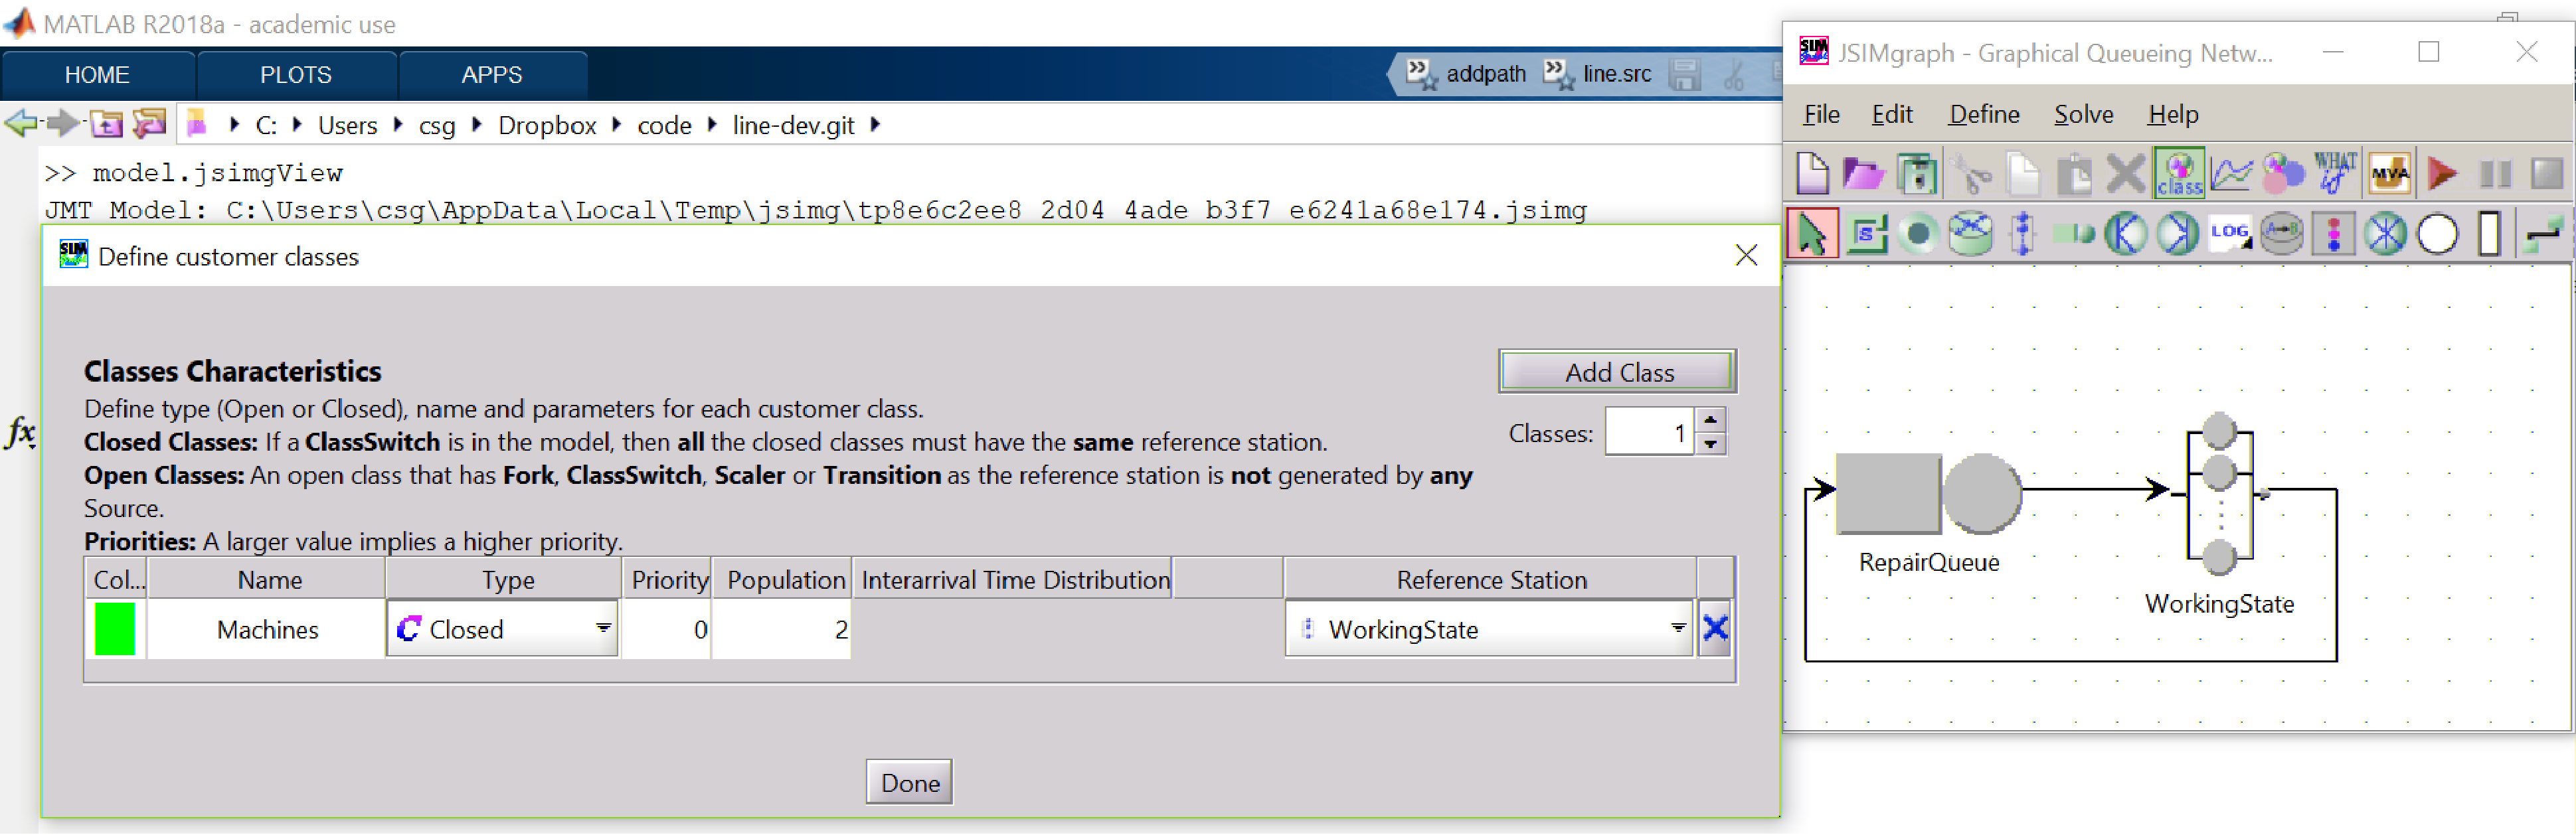
\includegraphics[width=14cm]{./images/jsimgViewFRP.pdf}
  \caption{Machine interference model in JSIMgraph}\label{FIG:jsimgViewFRP}
\end{figure}

We can now also inspect the CTMC more in the details as follows
\begin{MATLAB}
\begin{lstlisting}[language = matlab]
StateSpace = model.stateSpace()
InfGen = full(solver.generator())
\end{lstlisting}
\end{MATLAB}
\begin{JAVA}
\begin{lstlisting}[language=java, basicstyle=\ttfamily\scriptsize]
Matrix stateSpace = solver.stateSpace().stateSpace;
stateSpace.print();
Matrix infGen = solver.generator().infGen;
infGen.print();
\end{lstlisting}
\end{JAVA}
\begin{KOTLIN}
\begin{lstlisting}[language=kotlin, basicstyle=\ttfamily\scriptsize]
val stateSpace = solver.stateSpace().stateSpace
stateSpace.print()
val infGen = solver.generator().infGen
infGen.print()
\end{lstlisting}
\end{KOTLIN}
\begin{PYTHON}
\begin{lstlisting}[language=python]
state_space, node_state_space = solver.state_space()
print(state_space)
inf_gen, event_filt = solver.generator()
print(inf_gen)
\end{lstlisting}
\end{PYTHON}
which produces in output the state space of the model and the infinitesimal generator\index{infinitesimal generator (CTMC generator matrix)|see{Network solvers}} of the CTMC
\begin{MATLAB}
\begin{lstlisting}[language = matlab]
StateSpace =
     0     1     2
     1     0     2
     2     0     1
     3     0     0
InfGen =
   -8.0000    8.0000         0         0
    0.5000   -8.5000    8.0000         0
         0    1.0000   -5.0000    4.0000
         0         0    1.5000   -1.5000
\end{lstlisting}
\end{MATLAB}
\begin{JAVA}
\begin{lstlisting}[basicstyle=\ttfamily\scriptsize]
[0  1  2 
 1  0  2 
 2  0  1 
 3  0  0]

[-8.0   8.0     0     0 
  0.5  -8.5   8.0     0 
    0   1.0  -5.0   4.0 
    0     0   1.5  -1.5]
\end{lstlisting}
\end{JAVA}
\begin{KOTLIN}
\begin{lstlisting}[basicstyle=\ttfamily\scriptsize]
[0  1  2 
 1  0  2 
 2  0  1 
 3  0  0]

[-8.0   8.0     0     0 
  0.5  -8.5   8.0     0 
    0   1.0  -5.0   4.0 
    0     0   1.5  -1.5]
\end{lstlisting}
\end{KOTLIN}
\begin{PYTHON}
\begin{lstlisting}[basicstyle=\ttfamily\scriptsize]
[[0. 1. 2.]
 [1. 0. 2.]
 [2. 0. 1.]
 [3. 0. 0.]]

[[-8.   8.   0.   0. ]
 [ 0.5 -8.5  8.   0. ]
 [ 0.   1.  -5.   4. ]
 [ 0.   0.   1.5 -1.5]]
\end{lstlisting}
\end{PYTHON}
For example, the first state (\texttt{0 1 2}) consists of two components: the initial \texttt{0} denotes the number of jobs in service in the \texttt{delay}, while the remaining part is the state of the FCFS \texttt{queue}. In the latter, the \texttt{1} means that a job of class 1 (the only class in this model) is in the waiting buffer, while the \texttt{2} means that there are two jobs in service at the \texttt{queue}.

As another example, the second state (\texttt{1 0 2}) is similar, but one job has completed at the {queue} and has then moved to the \texttt{delay}, concurrently triggering an admission in service for the job that was in the queue buffer. As a result of this, the buffer is now empty. The corresponding transition rate in the infinitesimal generator matrix is  row $1$ and column $2$ of \Matlab{\texttt{InfGen}}\Java{\texttt{infGen}}\Kotlin{\texttt{infGen}}\Python{\texttt{inf\_gen}}, which has value $8.0$, that is the sum of the completion rates at the queue for each server in the first state, and where indexes 1 and 2 are the rows in \Matlab{\texttt{StateSpace}}\Java{\texttt{stateSpace}}\Kotlin{\texttt{stateSpace}}\Python{\texttt{state\_space}} associated to the source and destination states.

On this and larger infinite generators, we may also list individual non-zero transitions as follows
\begin{MATLAB}
\begin{lstlisting}[language = matlab]
>> model.printInfGen(InfGen,StateSpace)
[0 1 2]->[1 0 2]: 8.000000
[1 0 2]->[0 1 2]: 0.500000
[1 0 2]->[2 0 1]: 8.000000
[2 0 1]->[1 0 2]: 1.000000
[2 0 1]->[3 0 0]: 4.000000
[3 0 0]->[2 0 1]: 1.500000
\end{lstlisting}
\end{MATLAB}
\begin{JAVA}
\begin{lstlisting}[language=java, basicstyle=\ttfamily\scriptsize]
CTMC.printInfGen(infGen, stateSpace);
\end{lstlisting}
which gives
\begin{lstlisting}[basicstyle=\ttfamily\scriptsize]
[ 0.0   1.0   2.0 ] -> [ 1.0   0.0   2.0 ] : 8.0
[ 1.0   0.0   2.0 ] -> [ 0.0   1.0   2.0 ] : 0.5
[ 1.0   0.0   2.0 ] -> [ 2.0   0.0   1.0 ] : 8.0
[ 2.0   0.0   1.0 ] -> [ 1.0   0.0   2.0 ] : 1.0
[ 2.0   0.0   1.0 ] -> [ 3.0   0.0   0.0 ] : 4.0
[ 3.0   0.0   0.0 ] -> [ 2.0   0.0   1.0 ] : 1.5
\end{lstlisting}
\end{JAVA}
\begin{KOTLIN}
\begin{lstlisting}[language=kotlin, basicstyle=\ttfamily\scriptsize]
CTMC.printInfGen(infGen, stateSpace);
\end{lstlisting}
which gives
\begin{lstlisting}[basicstyle=\ttfamily\scriptsize]
[ 0.0   1.0   2.0 ] -> [ 1.0   0.0   2.0 ] : 8.0
[ 1.0   0.0   2.0 ] -> [ 0.0   1.0   2.0 ] : 0.5
[ 1.0   0.0   2.0 ] -> [ 2.0   0.0   1.0 ] : 8.0
[ 2.0   0.0   1.0 ] -> [ 1.0   0.0   2.0 ] : 1.0
[ 2.0   0.0   1.0 ] -> [ 3.0   0.0   0.0 ] : 4.0
[ 3.0   0.0   0.0 ] -> [ 2.0   0.0   1.0 ] : 1.5
\end{lstlisting}
\end{KOTLIN}
\begin{PYTHON}
\begin{lstlisting}[language=python]
CTMC.print_inf_gen(inf_gen, state_space)
\end{lstlisting}
gives
\begin{lstlisting}[basicstyle=\ttfamily\scriptsize]
[ 0.0   1.0   2.0 ] -> [ 1.0   0.0   2.0 ] : 8.0
[ 1.0   0.0   2.0 ] -> [ 0.0   1.0   2.0 ] : 0.5
[ 1.0   0.0   2.0 ] -> [ 2.0   0.0   1.0 ] : 8.0
[ 2.0   0.0   1.0 ] -> [ 1.0   0.0   2.0 ] : 1.0
[ 2.0   0.0   1.0 ] -> [ 3.0   0.0   0.0 ] : 4.0
[ 3.0   0.0   0.0 ] -> [ 2.0   0.0   1.0 ] : 1.5
\end{lstlisting}
\end{PYTHON}
The above printout helps in matching the state transitions to their rates.


To avoid having to inspect the \Matlab{\texttt{StateSpace}}\Java{\texttt{stateSpace}}\Kotlin{\texttt{stateSpace}}\Python{\texttt{state\_space}} variable to determine to which station a particular column refers to, we can alternatively use the more general invocation
\begin{MATLAB}
\begin{lstlisting}[language = matlab]
>> [StateSpace,nodeStateSpace] = solver.stateSpace();
>> nodeStateSpace{delay}
ans =
     0
     1
     2
     3
>> nodeStateSpace{queue}
ans =
     1     2
     0     2
     0     1
     0     0
\end{lstlisting}
\end{MATLAB}
\begin{JAVA}
\begin{lstlisting}[language=java, basicstyle=\ttfamily\scriptsize]
localStateSpace.print();
\end{lstlisting}
gives
\begin{lstlisting}[basicstyle=\ttfamily\scriptsize]
[0 
 1 
 2 
 3]

[1  2 
 0  2 
 0  1 
 0  0]
\end{lstlisting}
\end{JAVA}
\begin{KOTLIN}
\begin{lstlisting}[language=kotlin, basicstyle=\ttfamily\scriptsize]
localStateSpace.print();
\end{lstlisting}
gives
\begin{lstlisting}[basicstyle=\ttfamily\scriptsize]
[0 
 1 
 2 
 3]

[1  2 
 0  2 
 0  1 
 0  0]
\end{lstlisting}
\end{KOTLIN}
\begin{PYTHON}
\begin{lstlisting}[language=python]
state_space, node_state_space = solver.state_space()
print(node_state_space)
\end{lstlisting}
gives
\begin{lstlisting}[basicstyle=\ttfamily\scriptsize]
{0: array([[0.],
           [1.],
           [2.],
           [3.]]), 
 1: array([[1., 2.],
           [0., 2.],
           [0., 1.],
           [0., 0.]])}
\end{lstlisting}
\end{PYTHON}
which automatically splits the state space into its constituent parts for each stateful node.

A further observation is that \Matlab{\texttt{model.stateSpace()}}\Java{\texttt{model.stateSpace()}}\Kotlin{\texttt{model.stateSpace()}}\Python{\texttt{model.state\_space()}} forces the regeneration of the state space at each invocation, whereas the equivalent function in the CTMC solver, \Matlab{\texttt{solver.stateSpace()}}\Java{\texttt{solver.stateSpace()}}\Kotlin{\texttt{solver.stateSpace()}}\Python{\texttt{solver.state\_space()}}, returns the state space cached during the solution of the CTMC.

\subsection{Tutorial 4: Round-robin load-balancing}
\label{example-4-round-robin-load-balancing}
\index{Load balancing|see{Network models}}
In this example we consider a system of two parallel processor-sharing queues and we wish to study the effect of load-balancing on the average performance of an open class of jobs. We begin as usual with the node block, where we now include a special node, called the \texttt{Router}, to control the routing of jobs from the source into the queues:
\begin{MATLAB}
\begin{lstlisting}[language = matlab, basicstyle=\ttfamily\scriptsize]]
model = Network('RRLB');
source = Source(model, 'Source');
lb = Router(model, 'LB');
queue1 = Queue(model, 'Queue1', SchedStrategy.PS);
queue2 = Queue(model, 'Queue2', SchedStrategy.PS);
sink  = Sink(model, 'Sink');
\end{lstlisting}
\end{MATLAB}
\begin{JAVA}
\begin{lstlisting}[language = java, basicstyle=\ttfamily\scriptsize]
Network model = new Network("RRLB");
Source source = new Source(model, "Source");
Router lb = new Router(model, "LB");
Queue queue1 = new Queue(model, "Queue1", SchedStrategy.PS);
Queue queue2 = new Queue(model, "Queue2", SchedStrategy.PS);
Sink sink = new Sink(model, "Sink");
\end{lstlisting}
\end{JAVA}
\begin{KOTLIN}
\begin{lstlisting}[language = kotlin, basicstyle=\ttfamily\scriptsize]
val model = Network("RRLB")
val source = Source(model, "Source")
val lb = Router(model, "LB")
val queue1 = Queue(model, "Queue1", SchedStrategy.PS)
val queue2 = Queue(model, "Queue2", SchedStrategy.PS)
val sink = Sink(model, "Sink")
\end{lstlisting}
\end{KOTLIN}
\begin{PYTHON}
\begin{lstlisting}[language = python, basicstyle=\ttfamily\scriptsize]]
model = Network('RRLB')
source = Source(model, 'Source')
lb = Router(model, 'LB')
queue1 = Queue(model, 'Queue1', SchedStrategy.PS)
queue2 = Queue(model, 'Queue2', SchedStrategy.PS)
sink = Sink(model, 'Sink')
\end{lstlisting}
\end{PYTHON}
Let us then define the class block by setting exponentially-distributed inter-arrival times and service times, e.g.,
\begin{MATLAB}
\begin{lstlisting}[language = matlab, basicstyle=\ttfamily\scriptsize]]
jobclass = OpenClass(model, 'Class1');
source.setArrival(jobclass, Exp(1));
queue1.setService(jobclass, Exp(2));
queue2.setService(jobclass, Exp(2));
\end{lstlisting}
\end{MATLAB}
\begin{JAVA}
\begin{lstlisting}[language = java, basicstyle=\ttfamily\scriptsize]
OpenClass jobclass = new OpenClass(model, "Class1");
source.setArrival(jobclass, new Exp(1.0));
queue1.setService(jobclass, new Exp(2.0));
queue2.setService(jobclass, new Exp(2.0));
\end{lstlisting}
\end{JAVA}
\begin{KOTLIN}
\begin{lstlisting}[language = kotlin, basicstyle=\ttfamily\scriptsize]
val jobclass = OpenClass(model, "Class1")
source.setArrival(jobclass, Exp(1.0))
queue1.setService(jobclass, Exp(2.0))
queue2.setService(jobclass, Exp(2.0))
\end{lstlisting}
\end{KOTLIN}
\begin{PYTHON}
\begin{lstlisting}[language = python]
jobclass = OpenClass(model, 'Class1')
source.set_arrival(jobclass, Exp(1.0))
queue1.set_service(jobclass, Exp(2.0))
queue2.set_service(jobclass, Exp(2.0))
\end{lstlisting}
\end{PYTHON}
We now wish to express the fact that the router applies a round-robin strategy to dispatch jobs to the queues. Since this is now a non-probabilistic routing strategy, we need to adopt a slightly different style to declare the routing topology as we cannot specific anymore routing probabilities. First, we indicate the connections between the nodes, using the \Matlab{\texttt{addLinks}}\Java{\texttt{addLinks}}\Kotlin{\texttt{addLinks}}\Python{\texttt{add\_links}} function:
\begin{MATLAB}
\begin{lstlisting}[language = matlab, basicstyle=\ttfamily\scriptsize]]
model.addLinks([source, lb;
                lb,     queue1;
                lb,     queue2;
                queue1, sink;
                queue2, sink]);
\end{lstlisting}
At this point, all nodes are automatically configured to route jobs with equal probabilities on the outgoing links (\texttt{RoutingStrategy.RAND} policy). If we solve the model at this point, we see that the response time at the queues is around $0.66 s$.
\begin{lstlisting}[language = matlab, basicstyle=\ttfamily\scriptsize]]
>> jmtAvgTable = JMT(model,'seed',23000).avgTable()
jmtAvgTable =
  3x7 table
    Station    JobClass     QLen       Util       RespT     ResidT      Tput
    _______    ________    _______    _______    _______    _______    _______
    Source      Class1           0          0          0          0     1.0135
    Queue1      Class1     0.31612    0.24682    0.65411    0.65411      0.501
    Queue2      Class1     0.33403    0.25076    0.68406    0.34203    0.50413
\end{lstlisting}
\end{MATLAB}
\begin{JAVA}
\begin{lstlisting}[language = java, basicstyle=\ttfamily\scriptsize]
model.addLinks(new Node[][]{
                {source, lb},
                {lb, queue1},
                {lb, queue2},
                {queue1, sink},
                {queue2, sink}
});
\end{lstlisting}
At this point, all nodes are automatically configured to route jobs with equal probabilities on the outgoing links (\texttt{RoutingStrategy.RAND} policy). If we solve the model at this point, we see that the response time at the queues is around $0.66 s$.
\begin{lstlisting}[language = java, basicstyle=\ttfamily\scriptsize]
new JMT(model, "seed", 23000).avgTable().print();
\end{lstlisting}
which gives
\begin{lstlisting}[language = java, basicstyle=\ttfamily\scriptsize]
Station   	JobClass  	QLen      	Util      	RespT     	ResidT    	ArvR      	Tput
--------------------------------------------------------------------------------------------
Source    	Class1    	0          	0          	0          	0          	0          	1.01349
Queue1    	Class1    	0.31612   	0.24682   	0.65411   	0.65411   	0.50144   	0.50100
Queue2    	Class1    	0.33403   	0.25076   	0.68406   	0.34203   	0.50446   	0.50413
--------------------------------------------------------------------------------------------
\end{lstlisting}
\end{JAVA}
\begin{KOTLIN}
\begin{lstlisting}[language = kotlin, basicstyle=\ttfamily\scriptsize]
model.addLinks(arrayOf(
                arrayOf(source, lb),
                arrayOf(lb, queue1),
                arrayOf(lb, queue2),
                arrayOf(queue1, sink),
                arrayOf(queue2, sink)
))
\end{lstlisting}
At this point, all nodes are automatically configured to route jobs with equal probabilities on the outgoing links (\texttt{RoutingStrategy.RAND} policy). If we solve the model at this point, we see that the response time at the queues is around $0.66 s$.
\begin{lstlisting}[language = kotlin, basicstyle=\ttfamily\scriptsize]
JMT(model, "seed", 23000).avgTable().print()
\end{lstlisting}
which gives
\begin{lstlisting}[language = kotlin, basicstyle=\ttfamily\scriptsize]
Station   	JobClass  	QLen      	Util      	RespT     	ResidT    	ArvR      	Tput
--------------------------------------------------------------------------------------------
Source    	Class1    	0          	0          	0          	0          	0          	1.01349
Queue1    	Class1    	0.31612   	0.24682   	0.65411   	0.65411   	0.50144   	0.50100
Queue2    	Class1    	0.33403   	0.25076   	0.68406   	0.34203   	0.50446   	0.50413
--------------------------------------------------------------------------------------------
\end{lstlisting}
\end{KOTLIN}
\begin{PYTHON}
\begin{lstlisting}[language = python, basicstyle=\ttfamily\scriptsize]]
model.add_links([[source, lb],
               [lb, queue1],
               [lb, queue2],
               [queue1, sink],
               [queue2, sink]])
\end{lstlisting}
At this point, all nodes are automatically configured to route jobs with equal probabilities on the outgoing links (\texttt{RoutingStrategy.RAND} policy). If we solve the model at this point, we see that the response time at the queues is around $0.66 s$.
\begin{lstlisting}[language = python, basicstyle=\ttfamily\scriptsize]]
print(JMT(model, seed=23000).avg_table())
\end{lstlisting}
which gives
\begin{lstlisting}[language = python, basicstyle=\ttfamily\scriptsize]
Station   	JobClass  	QLen      	Util      	RespT     	ResidT    	ArvR      	Tput
--------------------------------------------------------------------------------------------
Source    	Class1    	0          	0          	0          	0          	0          	1.01349
Queue1    	Class1    	0.31612   	0.24682   	0.65411   	0.32706   	0.50144   	0.50100
Queue2    	Class1    	0.33403   	0.25076   	0.68406   	0.34203   	0.50446   	0.50413
--------------------------------------------------------------------------------------------
\end{lstlisting}
\end{PYTHON}
After resetting the internal data structures, which is required before modifying a model we can require \textsc{Line} to solve again the model using this time a round-robin policy at the router.
\begin{MATLAB}
\begin{lstlisting}[language = matlab, basicstyle=\ttfamily\scriptsize]]
model.reset()
lb.setRouting(jobclass, RoutingStrategy.RROBIN);
\end{lstlisting}
\end{MATLAB}
\begin{JAVA}
\begin{lstlisting}[language = java, basicstyle=\ttfamily\scriptsize]
model.reset();
lb.setRouting(jobclass, RoutingStrategy.RROBIN);
\end{lstlisting}
\end{JAVA}
\begin{KOTLIN}
\begin{lstlisting}[language = kotlin, basicstyle=\ttfamily\scriptsize]
model.reset()
lb.setRouting(jobclass, RoutingStrategy.RROBIN)
\end{lstlisting}
\end{KOTLIN}
\begin{PYTHON}
\begin{lstlisting}[language = python, basicstyle=\ttfamily\scriptsize]]
model.reset()
lb.set_routing(jobclass, RoutingStrategy.RROBIN)
\end{lstlisting}
\end{PYTHON}
A representation of the model at this point is shown in Figure~\ref{FIG:jsimgViewLB}.

\begin{figure}[t!]
  \centering
  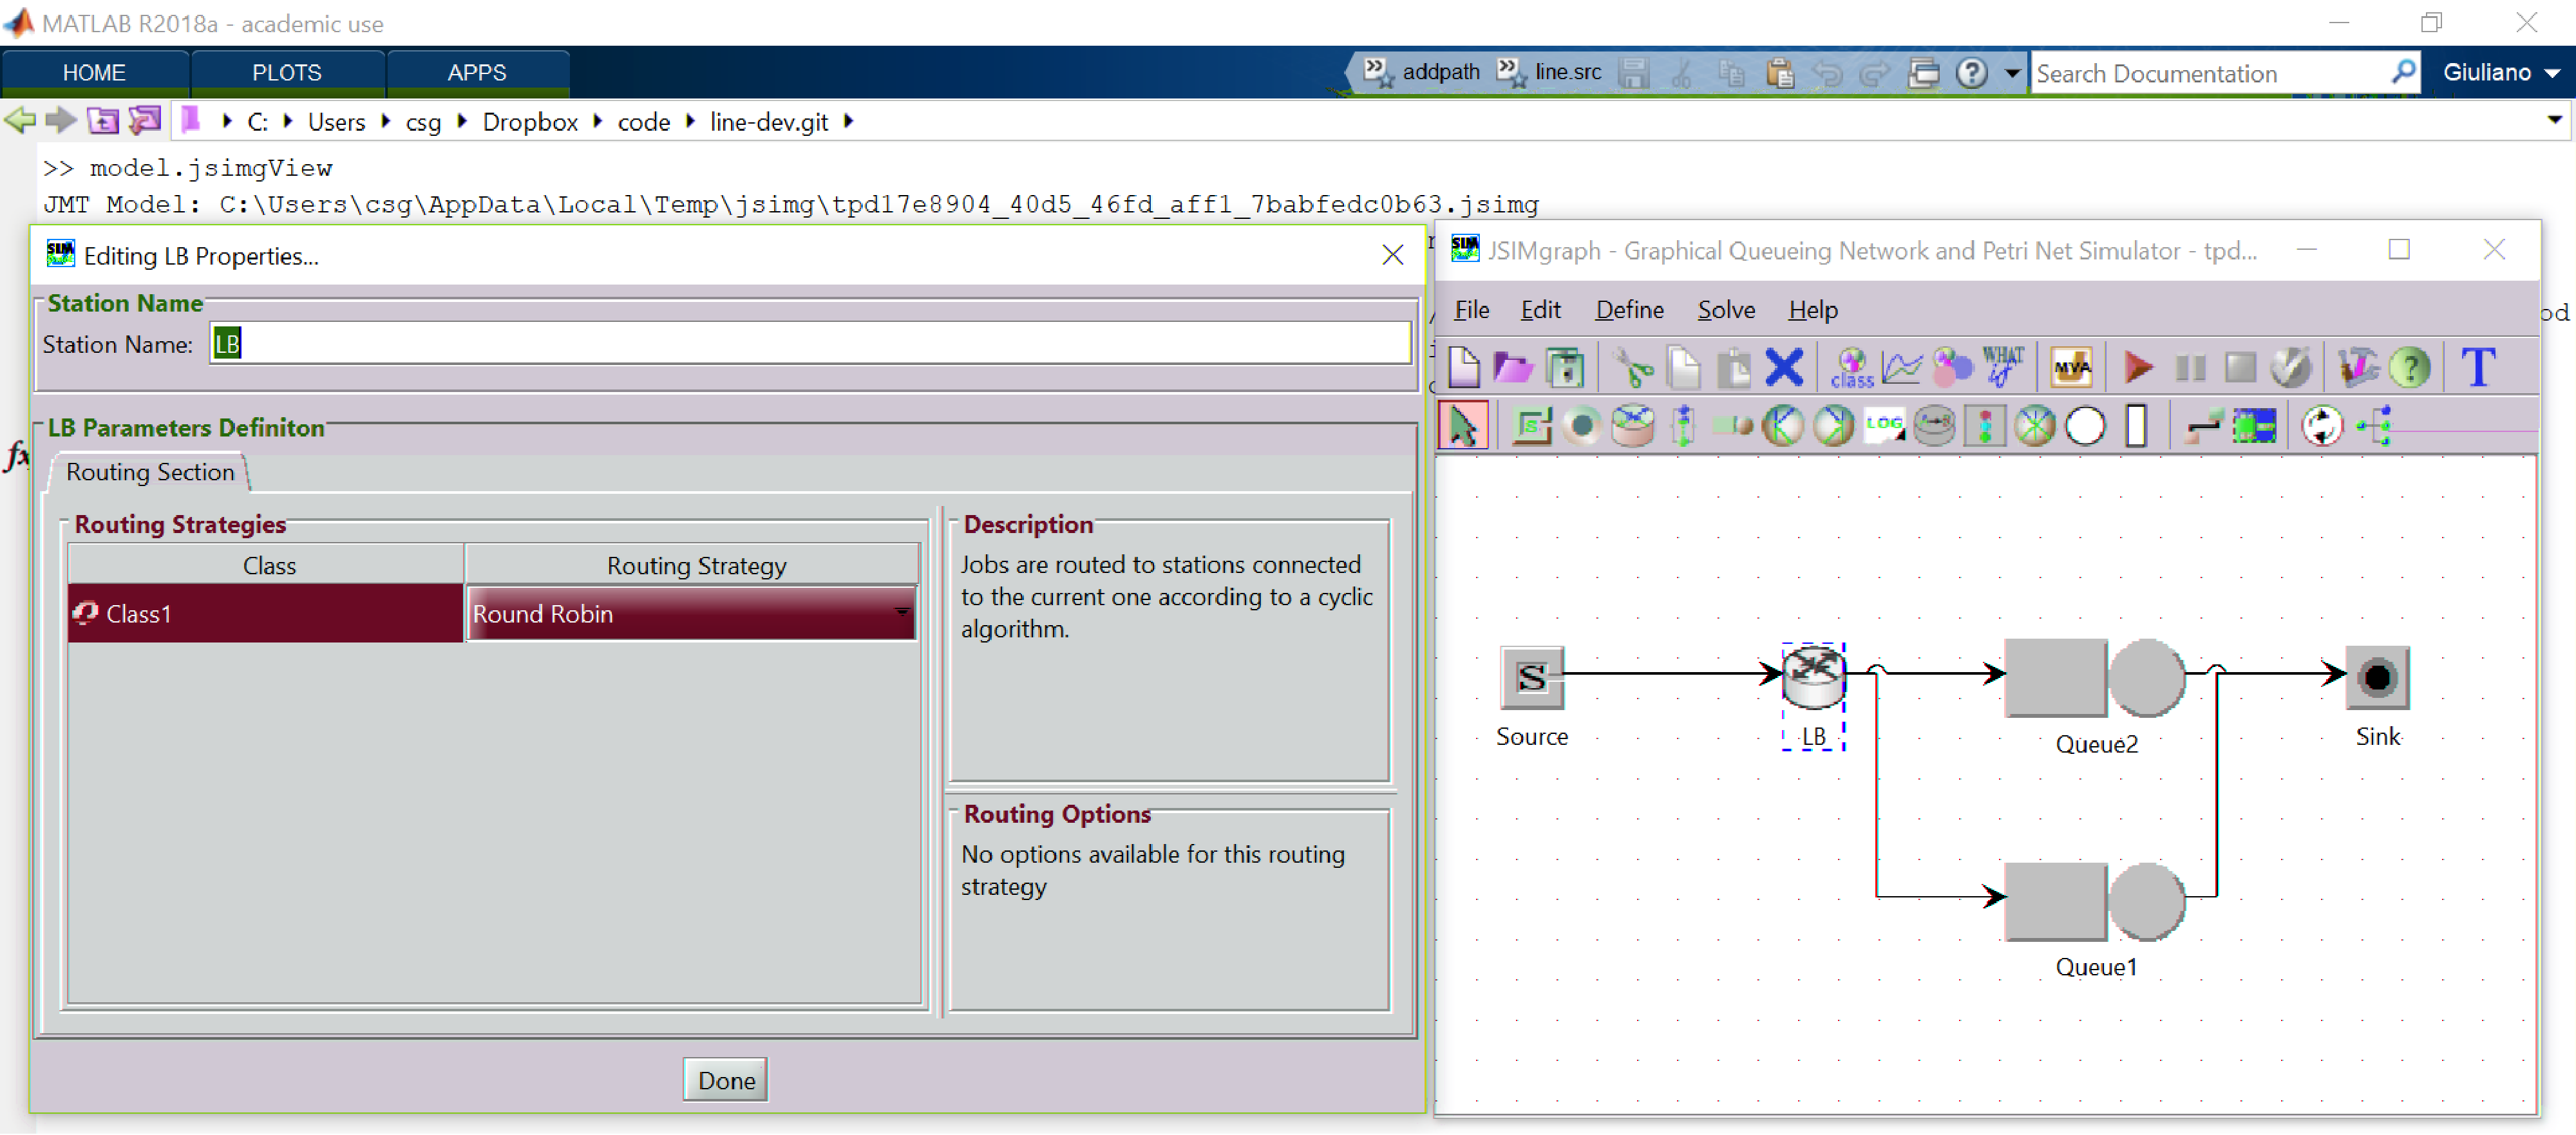
\includegraphics[width=14cm]{./images/jsimgViewLB.pdf}
  \caption{Load-balancing model}\label{FIG:jsimgViewLB}
\end{figure}

Lastly, we run again JMT and find that round-robin produces a visible decrease in response times, which are now around $0.56s$.
\begin{MATLAB}
\begin{lstlisting}[language = matlab]
>> jmtAvgTableRR = JMT(model,'seed',23000).avgTable()
jmtAvgTableRR =
  3x7 table
    Station    JobClass     QLen       Util       RespT     ResidT      Tput
    _______    ________    _______    _______    _______    _______    _______
    Source      Class1           0          0          0          0     1.0089
    Queue1      Class1     0.30429    0.26118    0.58482    0.58482    0.50526
    Queue2      Class1     0.29282    0.24397    0.57293    0.28647    0.50526
\end{lstlisting}
\end{MATLAB}
\begin{JAVA}
\begin{lstlisting}[language = java, basicstyle=\ttfamily\scriptsize]
new JMT(model, "seed", 23000).avgTable().print();
\end{lstlisting}
which gives
\begin{lstlisting}[language = java, basicstyle=\ttfamily\scriptsize]
Station   	JobClass  	QLen      	Util      	RespT     	ResidT    	ArvR      	Tput
--------------------------------------------------------------------------------------------
Source    	Class1    	0          	0          	0          	0          	0          	1.00887
Queue1    	Class1    	0.30429   	0.26118   	0.58482   	0.58482   	0.50290   	0.50526
Queue2    	Class1    	0.29282   	0.24397   	0.57293   	0.28647   	0.50496   	0.50526
--------------------------------------------------------------------------------------------
\end{lstlisting}
\end{JAVA}
\begin{KOTLIN}
\begin{lstlisting}[language = kotlin, basicstyle=\ttfamily\scriptsize]
JMT(model, "seed", 23000).avgTable().print()
\end{lstlisting}
which gives
\begin{lstlisting}[language = kotlin, basicstyle=\ttfamily\scriptsize]
Station   	JobClass  	QLen      	Util      	RespT     	ResidT    	ArvR      	Tput
--------------------------------------------------------------------------------------------
Source    	Class1    	0          	0          	0          	0          	0          	1.00887
Queue1    	Class1    	0.30429   	0.26118   	0.58482   	0.58482   	0.50290   	0.50526
Queue2    	Class1    	0.29282   	0.24397   	0.57293   	0.28647   	0.50496   	0.50526
--------------------------------------------------------------------------------------------
\end{lstlisting}
\end{KOTLIN}
\begin{PYTHON}
\begin{lstlisting}[language = python]
print(JMT(model, seed=23000).avg_table())
\end{lstlisting}
gives
\begin{lstlisting}[language = python]
  Station JobClass      QLen      Util     RespT    ResidT      ArvR      Tput
0  Source   Class1  0         0         0         0         1.008868  1.008868
1  Queue1   Class1  0.304291  0.261181  0.584815  0.292408  0.505255  0.505255
2  Queue2   Class1  0.292822  0.243971  0.572931  0.286466  0.505264  0.505264
\end{lstlisting}
\end{PYTHON}

\subsection{Tutorial 5: Modelling a re-entrant line}
\label{example-5-modelling-a-re-entrant-line}
Let us now consider a simple example inspired to the classic problem of modeling {\em re-entrant lines}. This arises in manufacturing systems where parts (i.e., jobs) re-enter multiple times a machine (i.e., a queueing station), asking at each visit a different class of service. This implies, for example, that the service time at every visit could feature a different mean or a different distribution compared to the previous visits, thus modeling a different stage of processing.

To illustrate this, consider for example a degenerate model composed of a single FCFS queue and $K$ classes. In this model, a job that completes processing in class $k$ is routed back at the tail of the queue in class $k+1$, unless $k=K$ in which case the job re-enters in class $1$.

We take the following assumptions: $K=3$ and class $k$ has an Erlang-2 service time distribution at the queue with mean equal to $k$; the system starts with $N_1=1$ jobs in class 1 and zero jobs in all other classes.
\begin{MATLAB}
\begin{lstlisting}[language = matlab]
model = Network('RL');
queue = Queue(model, 'Queue', SchedStrategy.FCFS);

K = 3; N = [1,0,0];
for k=1:K
    jobclass{k} = ClosedClass(model, ['Class',int2str(k)], N(k), queue);
    queue.setService(jobclass{k}, Erlang.fitMeanAndOrder(k,2));
end

P = model.initRoutingMatrix();
P{jobclass{1},jobclass{2}}(queue,queue) = 1.0;
P{jobclass{2},jobclass{3}}(queue,queue) = 1.0;
P{jobclass{3},jobclass{1}}(queue,queue) = 1.0;
model.link(P);
\end{lstlisting}
\end{MATLAB}
\begin{JAVA}
\begin{lstlisting}[language = java, basicstyle=\ttfamily\scriptsize]
Network model = new Network("RL");
Queue queue = new Queue(model, "Queue", SchedStrategy.FCFS);

ClosedClass jobClass1 = new ClosedClass(model, "Class1", 1, queue);
ClosedClass jobClass2 = new ClosedClass(model, "Class2", 0, queue);
ClosedClass jobClass3 = new ClosedClass(model, "Class3", 0, queue);

queue.setService(jobClass1, Erlang.fitMeanAndOrder(1, 2));
queue.setService(jobClass2, Erlang.fitMeanAndOrder(2, 2));
queue.setService(jobClass3, Erlang.fitMeanAndOrder(3, 2));

Matrix P = model.initRoutingMatrix();
P.set(jobClass1, jobClass2, queue, queue, 1.0);
P.set(jobClass2, jobClass3, queue, queue, 1.0);
P.set(jobClass3, jobClass1, queue, queue, 1.0);
model.link(P);
\end{lstlisting}
\end{JAVA}
\begin{KOTLIN}
\begin{lstlisting}[language = kotlin, basicstyle=\ttfamily\scriptsize]
val model = Network("RL")
val queue = Queue(model, "Queue", SchedStrategy.FCFS)

val jobClass1 = ClosedClass(model, "Class1", 1, queue)
val jobClass2 = ClosedClass(model, "Class2", 0, queue)
val jobClass3 = ClosedClass(model, "Class3", 0, queue)

queue.setService(jobClass1, Erlang.fitMeanAndOrder(1, 2))
queue.setService(jobClass2, Erlang.fitMeanAndOrder(2, 2))
queue.setService(jobClass3, Erlang.fitMeanAndOrder(3, 2))

val P = model.initRoutingMatrix()
P.set(jobClass1, jobClass2, queue, queue, 1.0)
P.set(jobClass2, jobClass3, queue, queue, 1.0)
P.set(jobClass3, jobClass1, queue, queue, 1.0)
model.link(P)
\end{lstlisting}
\end{KOTLIN}
\begin{PYTHON}
\begin{lstlisting}[language = python]
model = Network('RL')
queue = Queue(model, 'Queue', SchedStrategy.FCFS)
K = 3
N = (1, 0, 0)
jobclass = []
for k in range(K):
    jobclass.append(ClosedClass(model, 'Class' + str(k), N[k], queue))
    queue.set_service(jobclass[k], Erlang.fit_mean_and_order(1+k, 2))
    
P = model.init_routing_matrix()
P.set(jobclass[0], jobclass[1], queue, queue, 1.0)
P.set(jobclass[1], jobclass[2], queue, queue, 1.0)
P.set(jobclass[2], jobclass[0], queue, queue, 1.0)
model.link(P)
\end{lstlisting}
\end{PYTHON}

\noindent The corresponding JMT model is shown in Figure~\ref{FIG:jsimgViewCS}, where it can be seen that the class-switching\index{Class switching|see{Network models}} rule is automatically enforced by introduction of a \texttt{ClassSwitch} node in the network.

\begin{figure}[t!]
  \centering
  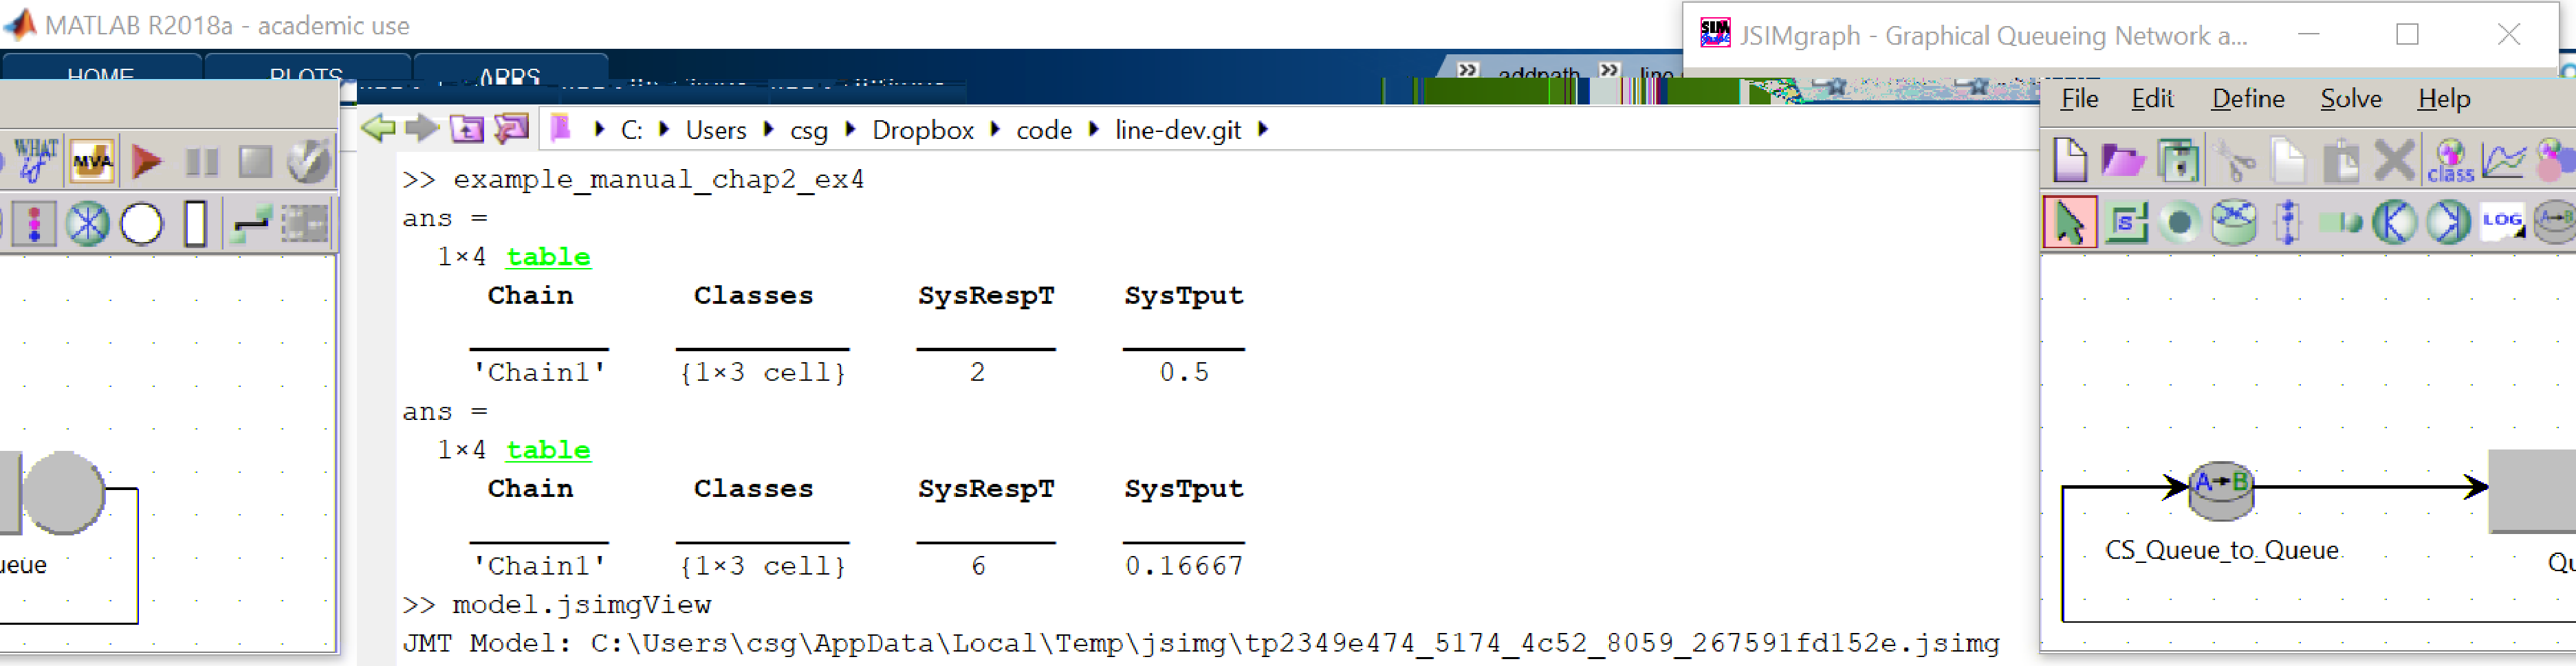
\includegraphics[width=14cm]{./images/jsimgViewCS.pdf}
  \caption{Re-entrant lines as an example of class-switching}
  \label{FIG:jsimgViewCS}
\end{figure}

\noindent We can now simulate the performance indexes for the different classes, for example using LINE's normalizing constant solver (\texttt{NC})
\begin{MATLAB}
\begin{lstlisting}[language = matlab]
>> ncAvgTable = NC(model).avgTable()
ncAvgTable =
    Station    JobClass     QLen       Util      RespT    ResidT      Tput
    _______    ________    _______    _______    _____    _______    _______
     Queue      Class1     0.16667    0.16667      1      0.33333    0.16667
     Queue      Class2     0.33333    0.33333      2      0.66667    0.16667
     Queue      Class3         0.5        0.5      3            1    0.16667
\end{lstlisting}
\end{MATLAB}
\begin{JAVA}
\begin{lstlisting}[language = java, basicstyle=\ttfamily\scriptsize]
 new NC(model).avgTable().print();
\end{lstlisting}
\begin{lstlisting}[language = java, basicstyle=\ttfamily\scriptsize]
NC(model).avgTable().print()
\end{lstlisting}
gives
\begin{lstlisting}[language = java, basicstyle=\ttfamily\scriptsize]
Station   	JobClass  	QLen      	Util      	RespT     	ResidT    	ArvR      	Tput      
--------------------------------------------------------------------------------------------
Queue     	Class1    	0.16667   	0.16667   	1.00000   	0.33333   	0.16667   	0.16667   
Queue     	Class2    	0.33333   	0.33333   	2.00000   	0.66667   	0.16667   	0.16667   
Queue     	Class3    	0.50000   	0.50000   	3.00000   	1.00000   	0.16667   	0.16667   
--------------------------------------------------------------------------------------------
\end{lstlisting}
\end{JAVA}
\begin{KOTLIN}
\begin{lstlisting}[language = kotlin, basicstyle=\ttfamily\scriptsize]
NC(model).avgTable().print()
\end{lstlisting}
gives
\begin{lstlisting}[language = kotlin, basicstyle=\ttfamily\scriptsize]
Station   	JobClass  	QLen      	Util      	RespT     	ResidT    	ArvR      	Tput      
--------------------------------------------------------------------------------------------
Queue     	Class1    	0.16667   	0.16667   	1.00000   	0.33333   	0.16667   	0.16667   
Queue     	Class2    	0.33333   	0.33333   	2.00000   	0.66667   	0.16667   	0.16667   
Queue     	Class3    	0.50000   	0.50000   	3.00000   	1.00000   	0.16667   	0.16667   
--------------------------------------------------------------------------------------------
\end{lstlisting}
\end{KOTLIN}
\begin{PYTHON}
\begin{lstlisting}[language = python]
ncAvgTable = NC(model).avg_table()
print(ncAvgTable)
\end{lstlisting}
gives
\begin{lstlisting}[language = python]
  Station JobClass      QLen      Util  RespT    ResidT  ArvR  Tput
0   Queue   Class1  0.166667  0.166667    1.0  0.333333   0.166667   0.166667
1   Queue   Class2  0.333333  0.333333    2.0  0.666667   0.166667   0.166667
2   Queue   Class3  0.500000  0.500000    3.0  1.000000   0.166667   0.166667
\end{lstlisting}
\end{PYTHON}
Suppose now that the job is considered completed, for the sake of computation of system performance metrics, only when it departs the queue in class $K$ (here \texttt{Class3}). By default, \textsc{Line} will return \emph{system-wide} performance metrics using the \Matlab{\texttt{avgSysTable}}\Java{\texttt{avgSysTable}}\Kotlin{\texttt{avgSysTable}}\Python{\texttt{avg\_sys\_table}} method, i.e.,
\begin{MATLAB}
\begin{lstlisting}[language = matlab]
>> ncAvgSysTable = NC(model).avgSysTable
ncAvgSysTable =
  1x4 table
    Chain        JobClasses        SysRespT    SysTput
    ______    _________________    ________    _______
    Chain1    {1x3 categorical}       2          0.5
\end{lstlisting}
\end{MATLAB}
\begin{KOTLIN}
\begin{lstlisting}[language = kotlin, basicstyle=\ttfamily\scriptsize]
NC(model).avgSysTable().print()
\end{lstlisting}
which gives
\begin{lstlisting}[language = kotlin, basicstyle=\ttfamily\scriptsize]
Chain       	 JobClasses  	         SysRespT  	         SysTput
-------------------------------------------------------------------------------
Chain0      	 (Class1 Class2 Class3)	 2.0000000000000000	 0.5000000000000000
-------------------------------------------------------------------------------
\end{lstlisting}
\end{KOTLIN}
\begin{JAVA}
\begin{lstlisting}[language = java, basicstyle=\ttfamily\scriptsize]
new NC(model).avgSysTable().print();
\end{lstlisting}
which gives
\begin{lstlisting}[language = java, basicstyle=\ttfamily\scriptsize]
Chain       	 JobClasses  	         SysRespT  	         SysTput
-------------------------------------------------------------------------------
Chain0      	 (Class1 Class2 Class3)	 2.0000000000000000	 0.5000000000000000
-------------------------------------------------------------------------------
\end{lstlisting}
\end{JAVA}
\begin{PYTHON}
\begin{lstlisting}[language = python]
ncAvgSysTable = NC(model).avg_sys_table()
print(ncAvgSysTable)
\end{lstlisting}
gives
\begin{lstlisting}[language = python]
    Chain              JobClasses  SysRespT  SysTput
0  Chain1  (Class1 Class2 Class3)       2.0      0.5
\end{lstlisting}
\end{PYTHON}
This method identifies the model \emph{chains}, i.e., groups of classes that can exchange jobs with each other, but not with classes in other chains. Since the job can switch into any of the three classes, in this model there is a single chain comprising the three classes.


\begin{MATLAB}
To see the composition of \texttt{Chain1}, we look at the second column entry
\begin{lstlisting}[language = matlab]
>> ncAvgSysTable.JobClasses{1}
ans =
  1x3 categorical array
     Class1      Class2      Class3
\end{lstlisting}
\end{MATLAB}

We see that the throughput of the chain is $0.5$, which means that \textsc{Line} is counting every departure from the queue in any class as a completion for the whole chain. This is incorrect for our model since we want to count completions only when jobs depart in \texttt{Class3}. To require this behavior, we can tell to the solver that passages for classes 1 and 2 through the reference station should not be counted as completions
\begin{MATLAB}
\begin{lstlisting}[language = matlab]
jobclass{1}.completes = false;
jobclass{2}.completes = false;
\end{lstlisting}
\end{MATLAB}
\begin{JAVA}
\begin{lstlisting}[language = java, basicstyle=\ttfamily\scriptsize]
jobClass1.setCompletes(false);
jobClass2.setCompletes(false);
\end{lstlisting}
\end{JAVA}
\begin{KOTLIN}
\begin{lstlisting}[language = kotlin, basicstyle=\ttfamily\scriptsize]
jobClass1.setCompletes(false)
jobClass2.setCompletes(false)
\end{lstlisting}
\end{KOTLIN}
\begin{PYTHON}
\begin{lstlisting}[language = python]
jobclass[0].completes = False
jobclass[1].completes = False
\end{lstlisting}
\end{PYTHON}

\noindent This modification then gives the correct chain throughput, matching the one of \texttt{Class3} alone
\begin{MATLAB}
\begin{lstlisting}[language = matlab]
>> ncAvgSysTable2 = NC(model).avgSysTable
ncAvgSysTable =
  1x4 table
    Chain        JobClasses        SysRespT    SysTput
    ______    _________________    ________    _______
    Chain1    {1x3 categorical}       6        0.16667
\end{lstlisting}
\end{MATLAB}
\begin{JAVA}
\begin{lstlisting}[language = java, basicstyle=\ttfamily\scriptsize]
new NC(model).avgSysTable().print();
\end{lstlisting}
\begin{lstlisting}[language = java, basicstyle=\ttfamily\scriptsize]
Chain       	 JobClasses  	         SysRespT  	         SysTput   
-------------------------------------------------------------------------------
Chain1      	 (Class1 Class2 Class3)	 6.0000000000000010	 0.1666666666666667
-------------------------------------------------------------------------------
\end{lstlisting}
\end{JAVA}
\begin{KOTLIN}
\begin{lstlisting}[language = kotlin, basicstyle=\ttfamily\scriptsize]
NC(model).avgSysTable().print()
\end{lstlisting}
\begin{lstlisting}[language = kotlin, basicstyle=\ttfamily\scriptsize]
Chain       	 JobClasses  	         SysRespT  	         SysTput   
-------------------------------------------------------------------------------
Chain1      	 (Class1 Class2 Class3)	 6.0000000000000010	 0.1666666666666667
-------------------------------------------------------------------------------
\end{lstlisting}
\end{KOTLIN}
\begin{PYTHON}
\begin{lstlisting}[language = python]
ncAvgSysTable = NC(model).avg_sys_table()
print(ncAvgSysTable)
\end{lstlisting}
gives
\begin{lstlisting}[language = python]
   Chain              JobClasses   SysRespT       SysTput
0  Chain1  (Class1 Class2 Class3)       6.0      0.166667
\end{lstlisting}
\end{PYTHON}

\subsection{Tutorial 6: A queueing network with caching}
\label{example-6-a-queueing-network-with-caching}
In this more advanced example, we show how to include in a queueing network a cache adopting a least-recently used (LRU) replacement policy. Under LRU, upon a cache miss the least-recently accessed item will be discarded to make room for the newly requested item.

We consider a cache with a capacity of 50 items, out of a set of 1000 cacheable items. Items are accessed by jobs visiting the cache according to a Zipf-like law\index{zipf distribution (popularity-based access)|see{Network models}} with exponent $\alpha=1.4$ and defined over the finite set of items. A client cyclically issues requests for the items, waiting for a reply before issuing the next request. We assume that a cache hit takes on average $0.2ms$ to process, while a cache hit takes $1ms$. We ask for the average request throughput of the system, differentiated across hits and misses.

\paragraph{Node block}
As usual, we begin by defining the nodes. Here a delay node will be used to describe the time spent by the requests in the system, while the cache node will determine hits and misses:
\begin{MATLAB}
\begin{lstlisting}[language = matlab]
model = Network('QNC');
% Block 1: nodes
clientDelay = Delay(model, 'Client');
cacheNode = Cache(model, 'Cache', 1000, 50, ReplacementStrategy.LRU);
cacheDelay = Delay(model, 'CacheDelay');
\end{lstlisting}
\end{MATLAB}
\begin{JAVA}
\begin{lstlisting}[language = java, basicstyle=\ttfamily\scriptsize]
Network model = new Network("QNC");
// Block 1: nodes
Delay clientDelay = new Delay(model, "Client");
Cache cacheNode = new Cache(model, "Cache", 1000, 50, ReplacementStrategy.LRU);
Delay cacheDelay = new Delay(model, "CacheDelay");
\end{lstlisting}
\end{JAVA}
\begin{KOTLIN}
\begin{lstlisting}[language = kotlin, basicstyle=\ttfamily\scriptsize]
val model = Network("QNC")
// Block 1: nodes
val clientDelay = Delay(model, "Client")
val cacheNode = Cache(model, "Cache", 1000, 50, ReplacementStrategy.LRU)
val cacheDelay = Delay(model, "CacheDelay")
\end{lstlisting}
\end{KOTLIN}
\begin{PYTHON}
\begin{lstlisting}[language = python]
model = Network('model')
client_delay = Delay(model, 'Client')
cache_node = Cache(model, 'Cache', 1000, 50, ReplacementStrategy.LRU)
cache_delay = Delay(model, 'CacheDelay')
\end{lstlisting}
\end{PYTHON}

\paragraph{Class block}
We define a set of classes to represent the incoming requests (\Matlab{\texttt{clientClass}}\Java{\texttt{clientClass}}\Kotlin{\texttt{clientClass}}\Python{\texttt{client\_class}}), cache hits (\Matlab{\texttt{hitClass}}\Java{\texttt{hitClass}}\Kotlin{\texttt{hitClass}}\Python{\texttt{hit\_class}}) and cache misses (\Matlab{\texttt{missClass}}\Java{\texttt{missClass}}\Kotlin{\texttt{missClass}}\Python{\texttt{miss\_class}}). These classes need to be closed to ensure that there is a single outstanding request from the client at all times:
\begin{MATLAB}
\begin{lstlisting}[language = matlab]
% Block 2: classes
clientClass = ClosedClass(model, 'ClientClass', 1, clientDelay, 0);
hitClass = ClosedClass(model, 'HitClass', 0, clientDelay, 0);
missClass = ClosedClass(model, 'MissClass', 0, clientDelay, 0);
\end{lstlisting}
\end{MATLAB}
\begin{JAVA}
\begin{lstlisting}[language = java, basicstyle=\ttfamily\scriptsize]
ClosedClass clientClass = new ClosedClass(model, "ClientClass", 1, clientDelay, 0);
ClosedClass hitClass = new ClosedClass(model, "HitClass", 0, clientDelay, 0);
ClosedClass missClass = new ClosedClass(model, "MissClass", 0, clientDelay, 0);
\end{lstlisting}
\end{JAVA}
\begin{KOTLIN}
\begin{lstlisting}[language = kotlin, basicstyle=\ttfamily\scriptsize]
val clientClass = ClosedClass(model, "ClientClass", 1, clientDelay, 0)
val hitClass = ClosedClass(model, "HitClass", 0, clientDelay, 0)
val missClass = ClosedClass(model, "MissClass", 0, clientDelay, 0)
\end{lstlisting}
\end{KOTLIN}
\begin{PYTHON}
\begin{lstlisting}[language = python]
client_class = ClosedClass(model, 'ClientClass', 1, client_delay, 0)
hit_class = ClosedClass(model, 'HitClass', 0, client_delay, 0)
miss_class = ClosedClass(model, 'MissClass', 0, client_delay, 0)
\end{lstlisting}
\end{PYTHON}
We then assign the processing times, using the \texttt{Immediate} distribution to ensure that the client issues immediately the request to the cache:
\begin{MATLAB}
\begin{lstlisting}[language = matlab]
clientDelay.setService(clientClass, Immediate());
cacheDelay.setService(hitClass, Exp.fitMean(0.2));
cacheDelay.setService(missClass, Exp.fitMean(1));
\end{lstlisting}
\end{MATLAB}
\begin{JAVA}
\begin{lstlisting}[language = java, basicstyle=\ttfamily\scriptsize]
clientDelay.setService(clientClass, new Immediate());
cacheDelay.setService(hitClass, Exp.fitMean(0.2));
cacheDelay.setService(missClass, Exp.fitMean(1.0));
\end{lstlisting}        
\end{JAVA}
\begin{KOTLIN}
\begin{lstlisting}[language = kotlin, basicstyle=\ttfamily\scriptsize]
clientDelay.setService(clientClass, Immediate())
cacheDelay.setService(hitClass, Exp.fitMean(0.2))
cacheDelay.setService(missClass, Exp.fitMean(1.0))
\end{lstlisting}
\end{KOTLIN}
\begin{PYTHON}
\begin{lstlisting}[language = python]
client_delay.set_service(client_class, Immediate())
cache_delay.set_service(hit_class, Exp.fit_mean(0.2))
cache_delay.set_service(miss_class, Exp.fit_mean(1.0))
\end{lstlisting}
\end{PYTHON}
The next step involves specifying that the request uses a Zipf-like distribution (with parameter $\alpha=1.4$) to select the item to read from the cache, out of a pool of 1000 items
\begin{MATLAB}
\begin{lstlisting}[language = matlab]
cacheNode.setRead(clientClass, Zipf(1.4,1000));
\end{lstlisting}
\end{MATLAB}
\begin{JAVA}
\begin{lstlisting}[language = java, basicstyle=\ttfamily\scriptsize]
cacheNode.setRead(clientClass, Zipf(1.4,1000));
\end{lstlisting}
\end{JAVA}
\begin{KOTLIN}
\begin{lstlisting}[language = kotlin, basicstyle=\ttfamily\scriptsize]
cacheNode.setRead(clientClass, Zipf(1.4, 1000))
\end{lstlisting}
\end{KOTLIN}
\begin{PYTHON}
\begin{lstlisting}[language = python]
cache_node.set_read(client_class, Zipf(1.4, 1000))
\end{lstlisting}
\end{PYTHON}
Finally, we ask that the job should become of class \Matlab{\texttt{hitClass}}\Java{\texttt{hitClass}}\Kotlin{\texttt{hitClass}}\Python{\texttt{hit\_class}} after a cache hit, and should become of class \Matlab{\texttt{missClass}}\Java{\texttt{missClass}}\Kotlin{\texttt{missClass}}\Python{\texttt{miss\_class}} after a cache miss:
\begin{MATLAB}
\begin{lstlisting}[language = matlab]
cacheNode.setHitClass(clientClass, hitClass);
cacheNode.setMissClass(clientClass, missClass);
\end{lstlisting}
\end{MATLAB}
\begin{JAVA}
\begin{lstlisting}[language = java, basicstyle=\ttfamily\scriptsize]
cacheNode.setHitClass(clientClass, hitClass);
cacheNode.setMissClass(clientClass, missClass);
\end{lstlisting}
\end{JAVA}
\begin{KOTLIN}
\begin{lstlisting}[language = kotlin, basicstyle=\ttfamily\scriptsize]
cacheNode.setHitClass(clientClass, hitClass)
cacheNode.setMissClass(clientClass, missClass)
\end{lstlisting}
\end{KOTLIN}
\begin{PYTHON}
\begin{lstlisting}[language = python]
cache_node.set_hit_class(client_class, hit_class)
cache_node.set_miss_class(client_class, miss_class)
\end{lstlisting}
\end{PYTHON}

\paragraph{Topology block}
Next, in the topology block we setup the routing so that the request, which starts in \Matlab{\texttt{clientClass}}\Java{\texttt{clientClass}}\Kotlin{\texttt{clientClass}}\Python{\texttt{client\_class}} at the \Matlab{\texttt{clientDelay}}\Java{\texttt{clientDelay}}\Kotlin{\texttt{clientDelay}}\Python{\texttt{client\_delay}}, then moves from there to the cache, remaining in \Matlab{\texttt{clientClass}}\Java{\texttt{clientClass}}\Kotlin{\texttt{clientClass}}\Python{\texttt{client\_class}}
\begin{MATLAB}
\begin{lstlisting}[language = matlab]
% Block 3: topology
P = model.initRoutingMatrix();
P{clientClass, clientClass}(clientDelay, cacheNode) = 1.0;
\end{lstlisting}
\end{MATLAB}
\begin{JAVA}
\begin{lstlisting}[language = java, basicstyle=\ttfamily\scriptsize]
Matrix P = model.initRoutingMatrix();
P.set(clientClass, clientClass, clientDelay, cacheNode, 1.0);
\end{lstlisting}
\end{JAVA}
\begin{KOTLIN}
\begin{lstlisting}[language = kotlin, basicstyle=\ttfamily\scriptsize]
val P = model.initRoutingMatrix()
P.set(clientClass, clientClass, clientDelay, cacheNode, 1.0)
\end{lstlisting}
\end{KOTLIN}
\begin{PYTHON}
\begin{lstlisting}[language = python]
P = model.init_routing_matrix()
P.set(client_class, client_class, client_delay, cache_node, 1.0)
\end{lstlisting}
\end{PYTHON}
Internally to the cache, the job will switch its class into either \Matlab{\texttt{hitClass}}\Java{\texttt{hitClass}}\Kotlin{\texttt{hitClass}}\Python{\texttt{hit\_class}} or \Matlab{\texttt{missClass}}\Java{\texttt{missClass}}\Kotlin{\texttt{missClass}}\Python{\texttt{miss\_class}}. Upon departure in one of these classes, we ask it to join in the same class \Matlab{\texttt{cacheDelay}}\Java{\texttt{cacheDelay}}\Kotlin{\texttt{cacheDelay}}\Python{\texttt{cache\_delay}} for further processing
\begin{MATLAB}
\begin{lstlisting}[language = matlab]
P{hitClass, hitClass}(cacheNode, cacheDelay) = 1.0;
P{missClass, missClass}(cacheNode, cacheDelay) = 1.0;
\end{lstlisting}
\end{MATLAB}
\begin{JAVA}
\begin{lstlisting}[language = java, basicstyle=\ttfamily\scriptsize]
P.set(hitClass, hitClass, cacheNode, cacheDelay, 1.0);
P.set(missClass, missClass, cacheNode, cacheDelay, 1.0);
\end{lstlisting}
\end{JAVA}
\begin{KOTLIN}
\begin{lstlisting}[language = kotlin, basicstyle=\ttfamily\scriptsize]
P.set(hitClass, hitClass, cacheNode, cacheDelay, 1.0)
P.set(missClass, missClass, cacheNode, cacheDelay, 1.0)
\end{lstlisting}
\end{KOTLIN}
\begin{PYTHON}
\begin{lstlisting}[language = python]
P.set(hit_class, hit_class, cache_node, cache_delay, 1.0)
P.set(miss_class, miss_class, cache_node, cache_delay, 1.0)
\end{lstlisting}
\end{PYTHON}
Lastly, the job returns to \Matlab{\texttt{clientDelay}}\Java{\texttt{clientDelay}}\Kotlin{\texttt{clientDelay}}\Python{\texttt{client\_delay}} for completion and start of a new request, which is done by switching its class back to \Matlab{\texttt{clientClass}}\Java{\texttt{clientClass}}\Kotlin{\texttt{clientClass}}\Python{\texttt{client\_class}}
\begin{MATLAB}
\begin{lstlisting}[language = matlab]
P{hitClass, clientClass}(cacheDelay, clientDelay) = 1.0;
P{missClass, clientClass}(cacheDelay, clientDelay) = 1.0;
\end{lstlisting}
\end{MATLAB}
\begin{JAVA}
\begin{lstlisting}[language = java, basicstyle=\ttfamily\scriptsize]
P.set(hitClass, clientClass, cacheDelay, clientDelay, 1.0);
P.set(missClass, clientClass, cacheDelay, clientDelay, 1.0);
\end{lstlisting}
\end{JAVA}
\begin{KOTLIN}
\begin{lstlisting}[language = kotlin, basicstyle=\ttfamily\scriptsize]
P.set(hitClass, clientClass, cacheDelay, clientDelay, 1.0)
P.set(missClass, clientClass, cacheDelay, clientDelay, 1.0)
\end{lstlisting}
\end{KOTLIN}
\begin{PYTHON}
\begin{lstlisting}[language = python]
P.set(hit_class, client_class, cache_delay, client_delay, 1.0)
P.set(miss_class, client_class, cache_delay, client_delay, 1.0)
\end{lstlisting}
\end{PYTHON}
The above routing strategy is finally applied to the model
\begin{MATLAB}
\begin{lstlisting}[language = matlab]
model.link(P);
\end{lstlisting}
\end{MATLAB}
\begin{JAVA}
\begin{lstlisting}[language = java, basicstyle=\ttfamily\scriptsize]
model.link(P);
\end{lstlisting}
\end{JAVA}
\begin{KOTLIN}
\begin{lstlisting}[language = kotlin, basicstyle=\ttfamily\scriptsize]
model.link(P)
\end{lstlisting}
\end{KOTLIN}
\begin{PYTHON}
\begin{lstlisting}[language = python]
model.link(P)
\end{lstlisting}
\end{PYTHON}

\paragraph{Solution block}
To solve the model, since JMT does not support cache modeling, we use the native simulation engine provided within \textsc{Line}, the \texttt{SSA} solver:

\begin{MATLAB}
\begin{lstlisting}[language = matlab]
% Block 4: solution
ssaAvgTable = SSA(model,'samples',2e4,'seed',1,'verbose',true).avgTable()
\end{lstlisting}
\end{MATLAB}
\begin{JAVA}
\begin{lstlisting}[language=java, basicstyle=\ttfamily\scriptsize]
ssaAvgTable = new SSA(model, "samples", 20000, "seed", 1, "verbose", true).avgTable();
\end{lstlisting}
\end{JAVA}
\begin{KOTLIN}
\begin{lstlisting}[language = kotlin, basicstyle=\ttfamily\scriptsize]
val ssaAvgTable = SSA(model, "samples", 20000, "seed", 1, "verbose", true).avgTable()
\end{lstlisting}
\end{KOTLIN}
\begin{PYTHON}
\begin{lstlisting}[language=python]
ssa_avg_table = SSA(model, samples=20000, seed=1, verbose=True).avg_table()
print(ssa_avg_table)
\end{lstlisting}
\end{PYTHON}
The above script produces the following result
\begin{MATLAB}
\begin{lstlisting}[language = matlab]
SSA samples:  20000
SSA analysis (method: default, lang: matlab) completed. 
ssaAvgTable =
  3x 8 table
     Station       JobClass       QLen       Util      RespT    ResidT     ArvR     Tput  
    __________    ___________    _______    _______    _____    _______    ____    _______
    Client        ClientClass          0          0    1e-08          0     0       2.8364
    CacheDelay    HitClass       0.43791    0.43791      0.2    0.15639     0       2.1895
    CacheDelay    MissClass      0.56209    0.56209        1    0.21803     0      0.56209
\end{lstlisting}
\end{MATLAB}
\begin{JAVA}
\begin{lstlisting}[language = java, basicstyle=\ttfamily\scriptsize]
SSA samples:   20000
SSA analysis (method: default, lang: java) completed.
Station     JobClass     QLen        Util        RespT       ResidT      ArvR        Tput        
-------------------------------------------------------------------------------------------------
Client      ClientClass  0           0           1.0e-08     0           0           2.91621     
CacheDelay  HitClass     0.47617     0.47617     0.20000     0.16524     0           2.38083     
CacheDelay  MissClass    0.52383     0.52383     1.00000     0.17380     0           0.52383     
-------------------------------------------------------------------------------------------------
\end{lstlisting}
\end{JAVA}
\begin{KOTLIN}
\begin{lstlisting}[language = kotlin, basicstyle=\ttfamily\scriptsize]
SSA samples:   20000
SSA analysis (method: default, lang: java) completed.
Station     JobClass     QLen        Util        RespT       ResidT      ArvR        Tput        
-------------------------------------------------------------------------------------------------
Client      ClientClass  0           0           1.0e-08     0           0           2.91621     
CacheDelay  HitClass     0.47617     0.47617     0.20000     0.16524     0           2.38083     
CacheDelay  MissClass    0.52383     0.52383     1.00000     0.17380     0           0.52383     
-------------------------------------------------------------------------------------------------
\end{lstlisting}
\end{KOTLIN}
\begin{PYTHON}
\begin{lstlisting}[basicstyle=\ttfamily\scriptsize]
SSA samples:   20000
SSA analysis (method: default, lang: java) completed. Runtime: 64.073000 seconds.
      Station     JobClass   QLen   Util       RespT  ResidT  ArvR    Tput
0      Client  ClientClass  0.000  0.000  1.0000e-08  0.0000   0.0  2.8059
4  CacheDelay     HitClass  0.436  0.436  2.0000e-01  0.1582   0.0  2.1801
5  CacheDelay    MissClass  0.564  0.564  1.0000e+00  0.2088   0.0  0.5640
\end{lstlisting}
\end{PYTHON}
The departing flows from the \Matlab{\texttt{cacheDelay}}\Java{\texttt{cacheDelay}}\Kotlin{\texttt{cacheDelay}}\Python{\texttt{cache\_delay}} are the miss and hit rates. Thus, the hit rate is $2.4554$ jobs per unit time, while the miss rate is $0.50892$ jobs per unit time.

Let us now suppose that we wish to verify the result with a longer simulation, for example with 10 times more samples. To this aim, we can use the automatic parallelization of \texttt{SSA} \Matlab{based on MATLAB's \texttt{spmd} construct}
\begin{MATLAB}
\begin{lstlisting}[language = matlab]
ssaAvgTablePara = SSA(model,'para','samples',2e4,'seed',1).avgTable()
\end{lstlisting}
\end{MATLAB}
\begin{JAVA}
\begin{lstlisting}[language=java, basicstyle=\ttfamily\scriptsize]
AvgTable ssaAvgTablePara = new SSA(model)
    .options()
    .method("parallel")
    .samples(20000)
    .seed(1)
    .build()
    .avgTable();
\end{lstlisting}
\end{JAVA}
\begin{KOTLIN}
\begin{lstlisting}[language=kotlin, basicstyle=\ttfamily\scriptsize]
val ssaAvgTablePara = SSA(model)
    .options()
    .method("parallel")
    .samples(20000)
    .seed(1)
    .build()
    .avgTable()
\end{lstlisting}
\end{KOTLIN}
\begin{PYTHON}
\begin{lstlisting}[language=python]
ssa_avg_table_para = SSA(model, samples=20000, seed=1).avg_table()
print(ssa_avg_table_para)
\end{lstlisting}
\end{PYTHON}
This gives us a rather similar result, when run on a dual-core machine
\begin{MATLAB}
\begin{lstlisting}[language = matlab]
Starting parallel pool (parpool) using the 'local' profile ...
connected to 2 workers.
ssaAvgTablePara =
 3x6 table
     Station       JobClass       QLen       Util      RespT    ResidT      Tput
    __________    ___________    _______    _______    _____    _______    _______
    Client        ClientClass          0          0       0           0     3.0652
    CacheDelay    HitClass       0.49871    0.49871     0.2     0.16689     2.4935
    CacheDelay    MissClass      0.50129    0.50129       1     0.16553    0.50129
\end{lstlisting}
\end{MATLAB}
\begin{JAVA}
\begin{lstlisting}[language=java, basicstyle=\ttfamily\scriptsize]
System.out.println(ssaAvgTablePara);
\end{lstlisting}
\end{JAVA}
\begin{KOTLIN}
\begin{lstlisting}[language=kotlin, basicstyle=\ttfamily\scriptsize]
System.out.println(ssaAvgTablePara);
\end{lstlisting}
\end{KOTLIN}
\begin{PYTHON}
\begin{lstlisting}[language=python]
print(ssa_avg_table_para)
\end{lstlisting}
\end{PYTHON}
The execution time is longer than usual at the first invocation of the parallel solver due to the time needed by MATLAB to bootstrap the parallel pool, in this example around 22 seconds. Successive invocations of parallel SSA normally take much less, with this example around 7 seconds each.

\subsection{Tutorial 7: Response time distribution and percentiles}
\label{example-7-response-time-distribution-and-percentiles}
In this example we illustrate the computation of response time percentiles in a queueing network model. We begin by instantiating a simple closed model consisting of a delay followed by a processor-sharing queueing station.
\begin{MATLAB}
\begin{lstlisting}[language = matlab]
model = Network('Model');
% Block 1: nodes
node{1} = Delay(model, 'Delay');
node{2} = Queue(model, 'Queue1', SchedStrategy.PS);
\end{lstlisting}
\end{MATLAB}
\begin{JAVA}
\begin{lstlisting}[language = java, basicstyle=\ttfamily\scriptsize]
Network model = new Network("Model");

Node[] node = new Node[2];
node[0] = new Delay(model, "Delay");
node[1] = new Queue(model, "Queue1", SchedStrategy.PS);
\end{lstlisting}
\end{JAVA}
\begin{KOTLIN}
\begin{lstlisting}[language = kotlin, basicstyle=\ttfamily\scriptsize]
val model = Network("Model")

val node = arrayOfNulls<Node>(2)
node[0] = Delay(model, "Delay")
node[1] = Queue(model, "Queue1", SchedStrategy.PS)
\end{lstlisting}
\end{KOTLIN}
\begin{PYTHON}
\begin{lstlisting}[language = python]
model = Network('Model')

node = np.empty(2, dtype=object)
node[0] = Delay(model, 'Delay')
node[1] = Queue(model, 'Queue1', SchedStrategy.PS)
\end{lstlisting}
\end{PYTHON}
There is a single class consisting of 5 jobs that circulate between the two stations, taking exponential service times at both.
\begin{MATLAB}
\begin{lstlisting}[language = matlab]
jobclass{1} = ClosedClass(model, 'Class1', 5, node{1}, 0);
node{1}.setService(jobclass{1}, Exp(1.0));
node{2}.setService(jobclass{1}, Exp(0.5));

model.link(Network.serialRouting(node{1},node{2}));
\end{lstlisting}
\end{MATLAB}
\begin{JAVA}
\begin{lstlisting}[language = java, basicstyle=\ttfamily\scriptsize]
JobClass[] jobclass = new JobClass[1];
jobclass[0] = new ClosedClass(model, "Class1", 5, (Station) node[0], 0);

((Delay) node[0]).setService(jobclass[0], new Exp(1.0));
((Queue) node[1]).setService(jobclass[0], new Exp(0.5));

model.link(Network.serialRouting(node[0],node[1]));
\end{lstlisting}
\end{JAVA}
\begin{KOTLIN}
\begin{lstlisting}[language = kotlin, basicstyle=\ttfamily\scriptsize]
val jobclass = arrayOfNulls<JobClass>(1)
jobclass[0] = ClosedClass(model, "Class1", 5, node[0] as Station, 0)

(node[0] as Delay).setService(jobclass[0]!!, Exp(1.0))
(node[1] as Queue).setService(jobclass[0]!!, Exp(0.5))

model.link(Network.serialRouting(node[0], node[1]))
\end{lstlisting}
\end{KOTLIN}
\begin{PYTHON}
\begin{lstlisting}[language = python]
jobclass = np.empty(2, dtype=object)
jobclass[0] = ClosedClass(model, 'Class1', 5, node[0], 0)
node[0].set_service(jobclass[0], Exp(1.0))
node[1].set_service(jobclass[0], Exp(0.5))

model.link(Network.serial_routing(node[0], node[1]))
\end{lstlisting}
\end{PYTHON}

We now wish to compare the response time distribution at the PS queue computed analytically with a fluid approximation against the simulated values returned by JMT. To do so, we call the \Matlab{\texttt{getCdfRespT}}\Java{\texttt{getCdfRespT}}\Kotlin{\texttt{getCdfRespT}}\Python{\texttt{cdf\_resp\_t}} method
\begin{MATLAB}
\begin{lstlisting}[language = matlab]
% Block 4: solution
RDfluid = FLD(model).cdfRespT();
RDsim = JMT(model,'seed',23000,'samples',1e4).cdfRespT();
\end{lstlisting}
\end{MATLAB}
\begin{JAVA}
\begin{lstlisting}[language=java, basicstyle=\ttfamily\scriptsize]
DistributionResult RDfluid = new FLD(model).cdfRespT();
DistributionResult RDsim = new JMT(model, "seed", 23000, "samples", 10000).cdfRespT();
\end{lstlisting}
\end{JAVA}
\begin{KOTLIN}
\begin{lstlisting}[language = kotlin, basicstyle=\ttfamily\scriptsize]
val RDfluid = FLD(model).cdfRespT()
val RDsim = JMT(model, "seed", 23000, "samples", 10000).cdfRespT()
\end{lstlisting}
\end{KOTLIN}
\begin{PYTHON}
\begin{lstlisting}[language=python]
rd_fluid = FLD(model).cdf_respt()
\end{lstlisting}
\begin{lstlisting}[language = python]
# rd_fluid = FLD(model).cdf_respt()
rd_sim = JMT(model, seed=23000, samples=10000).cdf_respt()
\end{lstlisting}
\end{PYTHON}
\Matlab{The returned data structures, \texttt{RDfluid} and \texttt{RDsim}, are cell arrays consisting of a 2-column matrix. The element in position $\{i,r\}$ of the cell array describes the response times at station $i$ for class $r$.}\Java{The returned data structures, \texttt{RDfluid} and \texttt{RDsim}, are Matrix arrays where element (i,r) describes the response times at station i for class r.}\Kotlin{The returned data structures, \texttt{RDfluid} and \texttt{RDsim}, are Matrix arrays where element (i,r) describes the response times at station i for class r.}\Python{The returned data structures, \texttt{rd\_fluid} and \texttt{rd\_sim}, are arrays where element [i,r] describes the response times at station i for class r.} \Matlab{The two columns within such matrices are defined similar to the output of \texttt{MATLAB}'s \texttt{ecdf} function}. The first column represents the cumulative distribution function (CDF) value $F(t)=Pr(T\leq t)$, where $T$ is the random variable denoting the response time, while $t$ is the percentile appearing in the corresponding entry of the second column.

\begin{MATLAB}
For example, to plot the complementary CDF $1-F(t)$ we can use the following code
\begin{lstlisting}[language = matlab]
% Plot results
semilogx(RDsim{2,1}(:,2),1-RDsim{2,1}(:,1),'r'); hold all;
semilogx(RDfluid{2,1}(:,2),1-RDfluid{2,1}(:,1),'--');
legend('jmt-transient','fluid-steady','Location','Best');
ylabel('Pr(T > t)'); xlabel('time t');
\end{lstlisting}
The graph shows that, although the simulation refers to a transient, while the fluid approximation refers to steady-state, there is a tight matching between the two response time distributions.
\end{MATLAB}
\begin{JAVA}
\end{JAVA}
\begin{KOTLIN}
\end{KOTLIN}
\begin{PYTHON}
For example, to plot the complementary CDF $1-F(t)$ we can use the following code
\begin{lstlisting}[language = python]
# Plotting in Python using matplotlib
import matplotlib.pyplot as plt
plt.semilogx(RDsim[1][0][:, 1], 1 - RDsim[1][0][:, 0], 'r', label='jmt-transient')
plt.semilogx(RDfluid[1][0][:, 1], 1 - RDfluid[1][0][:, 0], '--', label='fluid-steady')
plt.legend()
plt.ylabel('Pr(T > t)')
plt.xlabel('time t')
plt.show()
\end{lstlisting}
\end{PYTHON}
which produces the graph shown in Figure~\ref{FIG:percentiles}.
\begin{figure}[t!]
  \centering
  \Matlab{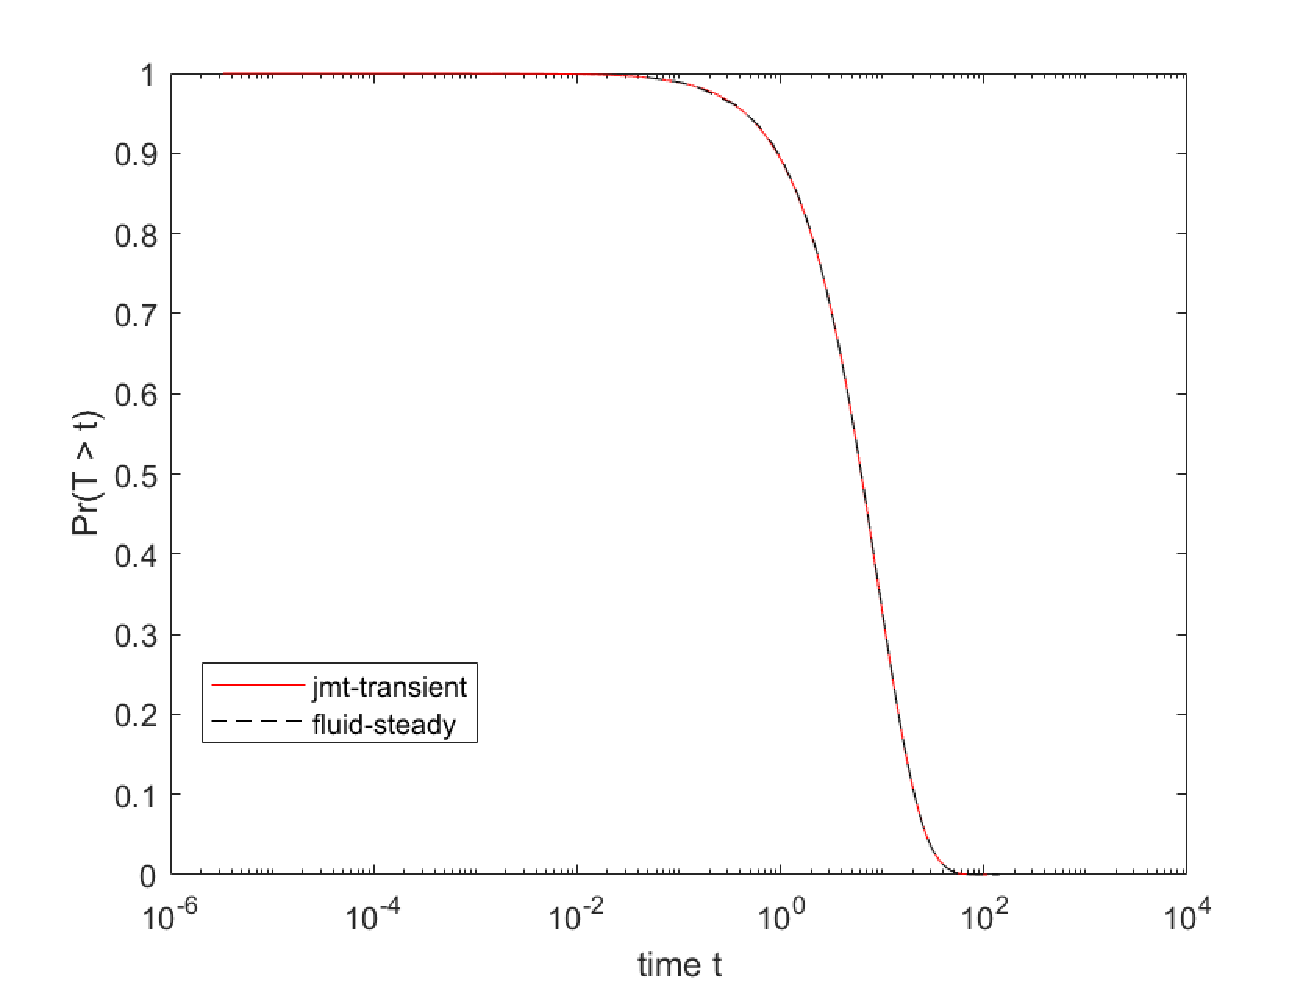
\includegraphics[width=7cm]{./images/percentiles.pdf}}
  \Java{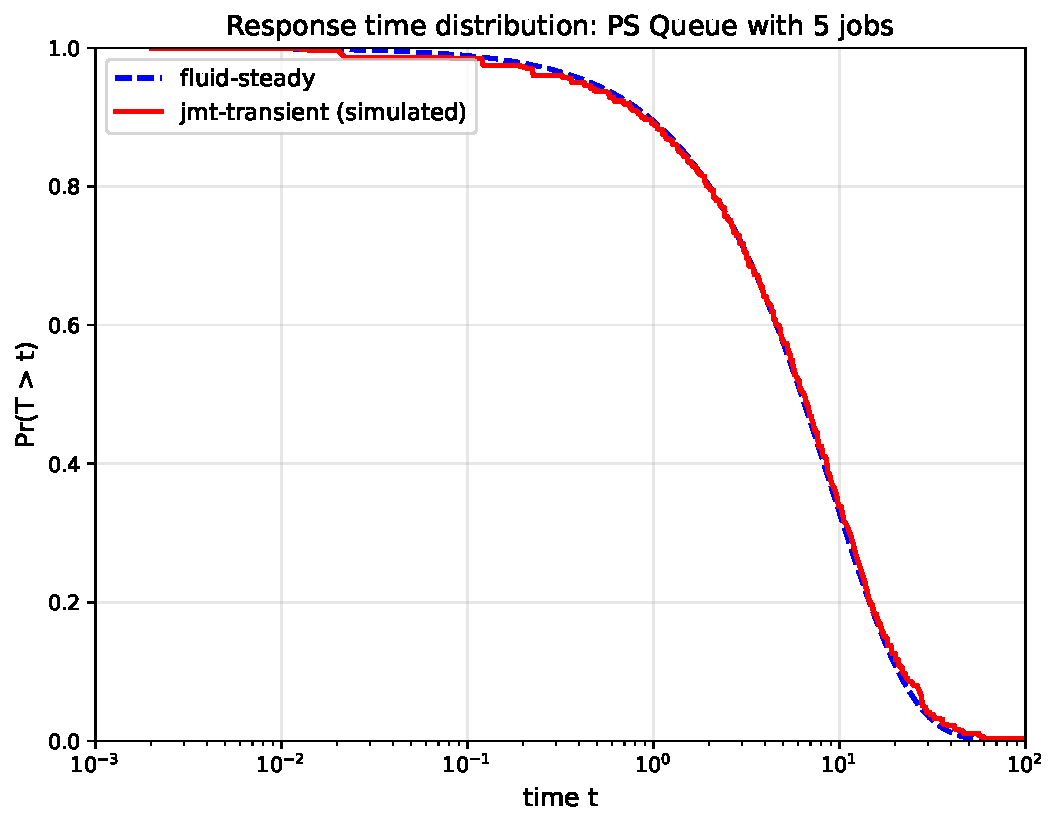
\includegraphics[width=7cm]{./images/percentiles_py.pdf}}
  \Kotlin{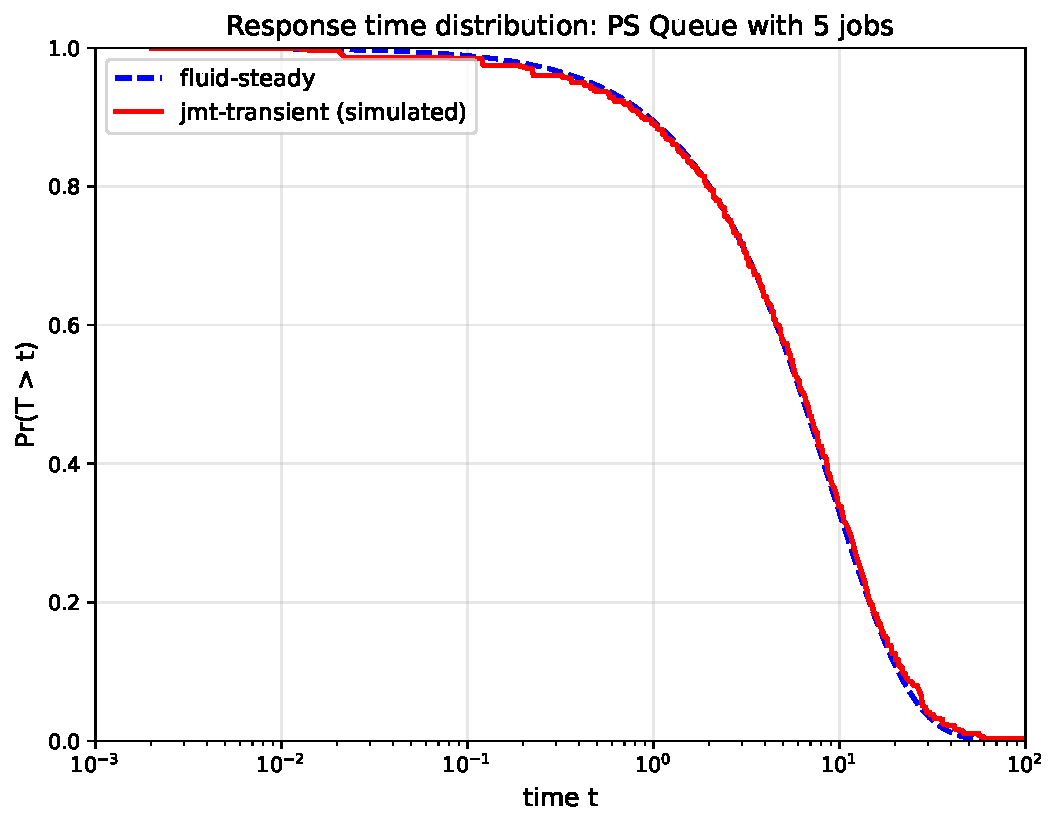
\includegraphics[width=7cm]{./images/percentiles_py.pdf}}
  \Python{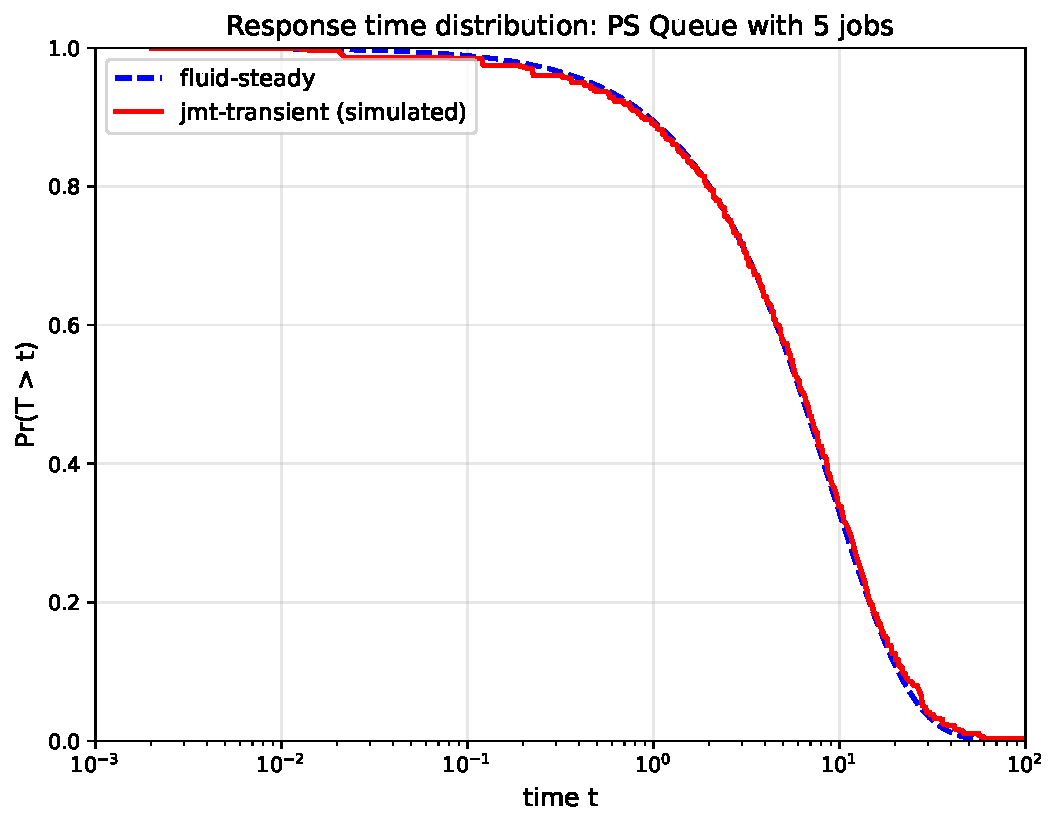
\includegraphics[width=7cm]{./images/percentiles_py.pdf}}
  \caption{Comparison of simulated response time distribution and its fluid approximation}
  \label{FIG:percentiles}
\end{figure}
The graph shows that, although the simulation refers to a transient, while the fluid approximation refers to steady-state, there is a tight matching between the two response time distributions.

We can readily compute the percentiles from the \Matlab{\texttt{RDfluid} and \texttt{RDsim}}\Java{\texttt{RDfluid} and \texttt{RDsim}}\Kotlin{\texttt{RDfluid} and \texttt{RDsim}}\Python{\texttt{rd\_fluid} and \texttt{rd\_sim}} data structures, e.g., for the 95th and 99th percentiles of the simulated distribution
\begin{MATLAB}
\begin{lstlisting}[language = python]
>> prc95=max(RDsim{2,1}(RDsim{2,1}(:,1)<0.95,2))
prc95 =
   27.0222
>> prc99=max(RDsim{2,1}(RDsim{2,1}(:,1)<0.99,2))
prc99 =
   41.8743
\end{lstlisting}
\end{MATLAB}
\begin{JAVA}
\begin{lstlisting}[language=java, basicstyle=\ttfamily\scriptsize]
// Calculate percentiles from CDF data
Matrix cdf = RDsim[1][0]; // Station 2, Class 1
double prc95 = 0, prc99 = 0;
for (int i = 0; i < cdf.getNumRows(); i++) {
    if (cdf.get(i, 0) < 0.95) {
        prc95 = cdf.get(i, 1);
    }
    if (cdf.get(i, 0) < 0.99) {
        prc99 = cdf.get(i, 1);
    }
}
System.out.println("95th percentile: " + prc95);
System.out.println("99th percentile: " + prc99);
\end{lstlisting}
\end{JAVA}
\begin{KOTLIN}
\begin{lstlisting}[language=kotlin, basicstyle=\ttfamily\scriptsize]
// Calculate percentiles from CDF data
val cdf = RDsim[1][0] // Station 2, Class 1
var prc95 = 0.0
var prc99 = 0.0
for (i in 0 until cdf.getNumRows()) {
    if (cdf.get(i, 0) < 0.95) {
        prc95 = cdf.get(i, 1)
    }
    if (cdf.get(i, 0) < 0.99) {
        prc99 = cdf.get(i, 1)
    }
}
println("95th percentile: $prc95")
println("99th percentile: $prc99")
\end{lstlisting}
\end{KOTLIN}
\begin{PYTHON}
\begin{lstlisting}[language = python]
# Calculate 95th and 99th percentiles from CDF data
cdf_data = RDsim[1][0]  # station 2, class 1
mask_95 = cdf_data[:, 0] < 0.95
prc95 = np.max(cdf_data[mask_95, 1]) if np.any(mask_95) else 0
mask_99 = cdf_data[:, 0] < 0.99
prc99 = np.max(cdf_data[mask_99, 1]) if np.any(mask_99) else 0
\end{lstlisting}
\end{PYTHON}
That is, 95\% of the response times at the PS queue (node 2, class 1) are less than or equal to 27.0222 time units, while 99\% are less than or equal to 41.8743 time units.
%\subsection{Tutorial 5: A two-layer network}

\subsection{Tutorial 8: Optimizing a performance metric}
\label{example-8-optimizing-a-performance-metric}
In this example, we show how to optimize with the help of \textsc{Line} a performance metric. We wish to find the optimal routing probabilities that minimize average response times for two parallel processor sharing queues. We assume that jobs are fed by a delay station, arranged with the two queues in a closed network topology.

\begin{MATLAB}
We first define a MATLAB function (e.g., \texttt{ex8.m}) with header
\begin{lstlisting}[language = matlab]
function p_star = ex8()
\end{lstlisting}
\end{MATLAB}
\begin{JAVA}
In this example, we use the \texttt{jcobyla} optimizer, which can be imported by including the following dependency in \texttt{pom.xml}:
\begin{lstlisting}[basicstyle=\ttfamily\scriptsize]
    <dependency>
      <groupId>de.xypron.jcobyla</groupId>
      <artifactId>jcobyla</artifactId>
      <version>1.3</version>
    </dependency>
\end{lstlisting}
\end{JAVA}
\begin{KOTLIN}
In this example, we use the \texttt{jcobyla} optimizer, which can be imported by including the following dependency in \texttt{pom.xml}:
\begin{lstlisting}[basicstyle=\ttfamily\scriptsize]
    <dependency>
      <groupId>de.xypron.jcobyla</groupId>
      <artifactId>jcobyla</artifactId>
      <version>1.3</version>
    </dependency>
\end{lstlisting}
\end{KOTLIN}
\begin{JAVA}
We will now define a queueing network model, called \texttt{routingModel}, which accepts a parameter describing a routing probability
\begin{lstlisting}[language=java, basicstyle=\ttfamily\scriptsize]
Calcfc objFun = new Calcfc() {
    @Override
    public double compute(int n, int m, double[] x, double[] con) {
        return routingModel.apply(x[0]) ;
    }
};
\end{lstlisting}
\end{JAVA}
\begin{KOTLIN}
We will now define a queueing network model, called \texttt{routingModel}, which accepts a parameter describing a routing probability
\begin{lstlisting}[language=kotlin, basicstyle=\ttfamily\scriptsize]
Calcfc objFun = new Calcfc() {
    @Override
    public double compute(int n, int m, double[] x, double[] con) {
        return routingModel.apply(x[0]) ;
    }
};
\end{lstlisting}
\end{KOTLIN}
\begin{PYTHON}
We first define a Python function with header
\begin{lstlisting}[language = python]
def objFun(p):
\end{lstlisting}
\end{PYTHON}
Within the function definition, we instantiate the two queues and the delay station
\begin{MATLAB}
\begin{lstlisting}[language = matlab]
model = Network('LoadBalCQN');
% Block 1: nodes
delay = Delay(model,'Think');
queue1 = Queue(model, 'Queue1', SchedStrategy.PS);
queue2 = Queue(model, 'Queue2', SchedStrategy.PS);
\end{lstlisting}
\end{MATLAB}
\begin{JAVA}
In the routing model, we instantiate the two queues and the delay station
\begin{lstlisting}[language = java, basicstyle=\ttfamily\scriptsize]
Network model = new Network("LoadBalCQN");
// Block 1: nodes
Delay delay = new Delay(model, "Think");
Queue queue1 = new Queue(model, "Queue1", SchedStrategy.PS);
Queue queue2 = new Queue(model, "Queue2", SchedStrategy.PS);
\end{lstlisting}
\end{JAVA}
\begin{KOTLIN}
\begin{lstlisting}[language = kotlin, basicstyle=\ttfamily\scriptsize]
val model = Network("LoadBalCQN")
// Block 1: nodes
val delay = Delay(model, "Think")
val queue1 = Queue(model, "Queue1", SchedStrategy.PS)
val queue2 = Queue(model, "Queue2", SchedStrategy.PS)
\end{lstlisting}
\end{KOTLIN}
\begin{PYTHON}
\begin{lstlisting}[language = python]
model = Network('LoadBalCQN')
delay = Delay(model, 'Think')
queue1 = Queue(model, 'Queue1', SchedStrategy.PS)
queue2 = Queue(model, 'Queue2', SchedStrategy.PS)
\end{lstlisting}
\end{PYTHON}
We assume that 16 jobs circulate among the nodes, and that the service rates are $\sigma=1$ jobs per unit time at the delay, and $\mu_1=0.75$ and $\mu_2=0.50$ at the two queues:
\begin{MATLAB}
\begin{lstlisting}[language = matlab]
% Block 2: classes
cclass = ClosedClass(model, 'Job1', 16, delay);
delay.setService(cclass, Exp(1));
queue1.setService(cclass, Exp(0.75));
queue2.setService(cclass, Exp(0.50));
\end{lstlisting}
\end{MATLAB}
\begin{JAVA}
\begin{lstlisting}[language = java, basicstyle=\ttfamily\scriptsize]
// Block 2: classes
ClosedClass cclass = new ClosedClass(model, "Job1", 16, delay);
delay.setService(cclass, new Exp(1));
queue1.setService(cclass, new Exp(0.75));
queue2.setService(cclass, new Exp(0.50));
\end{lstlisting}
\end{JAVA}
\begin{KOTLIN}
\begin{lstlisting}[language = kotlin, basicstyle=\ttfamily\scriptsize]
// Block 2: classes
val cclass = ClosedClass(model, "Job1", 16, delay)
delay.setService(cclass, Exp(1))
queue1.setService(cclass, Exp(0.75))
queue2.setService(cclass, Exp(0.50))
\end{lstlisting}
\end{KOTLIN}
\begin{PYTHON}
\begin{lstlisting}[language = python]
cclass = ClosedClass(model, 'Job1', 16, delay)
delay.set_service(cclass, Exp(1))
queue1.set_service(cclass, Exp(0.75))
queue2.set_service(cclass, Exp(0.50))
\end{lstlisting}
\end{PYTHON}
We initially setup a topology with arbitrary values for the routing probabilities between delay and queues, ensuring that jobs completing at the queues return to the delay:
\begin{MATLAB}
\begin{lstlisting}[language = matlab]
% Block 3: topology
P = model.initRoutingMatrix();
P{cclass}(queue1, delay) = 1.0;
P{cclass}(queue2, delay) = 1.0;
model.link(P);
\end{lstlisting}
\end{MATLAB}
\begin{JAVA}
\begin{lstlisting}[language = java, basicstyle=\ttfamily\scriptsize]
Matrix P = model.initRoutingMatrix();
P.set(cclass, queue1, delay, 1.0);
P.set(cclass, queue2, delay, 1.0);
model.link(P);
\end{lstlisting}
\end{JAVA}
\begin{KOTLIN}
\begin{lstlisting}[language = kotlin, basicstyle=\ttfamily\scriptsize]
val P = model.initRoutingMatrix()
P.set(cclass, queue1, delay, 1.0)
P.set(cclass, queue2, delay, 1.0)
model.link(P)
\end{lstlisting}
\end{KOTLIN}
\begin{PYTHON}
\begin{lstlisting}[language = python]
P = model.init_routing_matrix()
P.set(cclass, cclass, queue1, delay, 1.0)
P.set(cclass, cclass, queue2, delay, 1.0)
model.link(P)
\end{lstlisting}
\end{PYTHON}
We now return the system response time for the jobs as a function of the routing probability $p$ to choose queue 1 instead of queue 2:
\begin{MATLAB}
\begin{lstlisting}[language = matlab]
% Block 4: solution
    function R = objFun(p)
        P{cclass}(delay, queue1) = p;
        P{cclass}(delay, queue2) = 1-p;
        model.link(P);
        R = MVA(model,'exact','verbose',false).avgSysRespT;
    end
\end{lstlisting}
Lastly, we optimize the function we defined
\begin{lstlisting}[language = matlab]
p_opt = fminbnd(@(p) objFun(p), 0,1)
\end{lstlisting}
In the above listing, \texttt{objFun} first updates the routing topology, prior to obtaining the corresponding system response time. To search for the optimal routing probability $p$, we have also used MATLAB's \texttt{fminbnd} which restricts the search range in the interval $[0,1]$.
\end{MATLAB}
\begin{JAVA}
\begin{lstlisting}[language = java, basicstyle=\ttfamily\scriptsize]
Function<Double, Double> routingModel = (p) -> {
    // Block 4: solution
    P.set(cclass, delay, queue1, p);
    P.set(cclass, delay, queue2, 1 - p);
    model.reset();
    model.link(P);
    MVA solver = new MVA(model, "exact");
    return (Double) solver.avgSysRespT().get(0);
};
\end{lstlisting}
\end{JAVA}
\begin{KOTLIN}
\begin{lstlisting}[language = kotlin, basicstyle=\ttfamily\scriptsize]
val routingModel = { p: Double ->
    // Block 4: solution
    P.set(cclass, delay, queue1, p)
    P.set(cclass, delay, queue2, 1 - p)
    model.reset()
    model.link(P)
    val solver = MVA(model, "exact")
    solver.avgSysRespT()[0] as Double
}
\end{lstlisting}
\end{KOTLIN}
Lastly, we optimize the function we defined
\begin{JAVA}
\begin{lstlisting}[language = java, basicstyle=\ttfamily\scriptsize]
Calcfc objFun = new Calcfc() {
    @Override
    public double compute(int n, int m, double[] x, double[] con) {
        return routingModel.apply(x[0]);
    }
};
double[] p = {0.5};
Cobyla.findMinimum(objFun, 1, 0, p, 0.5, 1.0e-8, 0, 10000);

System.out.println("Optimal p: " + p[0]);
\end{lstlisting}
\end{JAVA}
\begin{KOTLIN}
\begin{lstlisting}[language = kotlin, basicstyle=\ttfamily\scriptsize]
val objFun = Calcfc { _, _, x, _ -> routingModel(x[0]) }
val p = doubleArrayOf(0.5)
Cobyla.findMinimum(objFun, 1, 0, p, 0.5, 1.0e-8, 0, 10000)

println("Optimal p: ${p[0]}")
\end{lstlisting}
\end{KOTLIN}
\begin{PYTHON}
\begin{lstlisting}[language = python]
def routing_model(p):
    # Block 4: solution
    P.set(cclass, cclass, delay, queue1, p)
    P.set(cclass, cclass, delay, queue2, 1.0 - p)
    model.reset()
    model.link(P)
    solver = MVA(model, method='exact')
    return solver.avg_sys_respt()[0]
\end{lstlisting}
Lastly, we optimize the function we defined
\begin{lstlisting}[language = python]
from scipy import optimize
p_opt = optimize.fminbound(routing_model, 0, 1)
print(f'Optimal p: {p_opt}')
\end{lstlisting}
\end{PYTHON}
\begin{MATLAB}
We are now ready to run \texttt{ex8}. The execution returns the optimal value $0.6104878504366782$.
\end{MATLAB}
\begin{JAVA}
We are now ready to run the example. The execution returns the optimal value $0.6104880200336327$.
\end{JAVA}
\begin{KOTLIN}
We are now ready to run the example. The execution returns the optimal value $0.6104880200336327$.
\end{KOTLIN}
\begin{PYTHON}
We are now ready to run the example. The execution returns the optimal value $0.6104878504366782$.
\end{PYTHON}

\subsection{Tutorial 9: Studying a departure process}
\label{example-9-studying-a-departure-process}
This examples illustrates \textsc{Line}'s support for extracting simulation data about particular events in an extended queueing network, such as departures from a particular queue.

Our goal is to obtain the squared coefficient of variation of the inter-departure times from a $M/E_2/1$ queue, which has Poisson arrivals and 2-phase Erlang distributed service times.

Because this is a classic model, we can find it in \textsc{Line}'s model gallery. The additional return parameters (e.g., \texttt{source},\texttt{queue}, ...) provide handles to the entities within the model.
\begin{MATLAB}
\begin{lstlisting}[language = matlab]
[model,source,queue,sink,jobclass] = gallery_merl1;
\end{lstlisting}
\end{MATLAB}
\begin{JAVA}
\begin{lstlisting}[language=java, basicstyle=\ttfamily\scriptsize]
model = gallery_merl1();
\end{lstlisting}
\end{JAVA}
\begin{KOTLIN}
\begin{lstlisting}[language = kotlin, basicstyle=\ttfamily\scriptsize]
val model = gallery_merl1()
\end{lstlisting}
\end{KOTLIN}
\begin{PYTHON}
\begin{lstlisting}[language = python]
model = gallery_merl1()
\end{lstlisting}
\end{PYTHON}
We now extract 50,000 samples from simulation based on the underpinning continuous-time Markov chain
\begin{MATLAB}
\begin{lstlisting}[language = matlab]
solver = CTMC(model,'cutoff',150,'seed',23000);
sa = solver.sampleSysAggr(1e5);
\end{lstlisting}
\end{MATLAB}
\begin{JAVA}
\begin{lstlisting}[language=java, basicstyle=\ttfamily\scriptsize]
solver = new CTMC(model, "cutoff", 150, "seed", 23000);
sa = solver.sampleSysAggr(100000);
\end{lstlisting}
\end{JAVA}
\begin{KOTLIN}
\begin{lstlisting}[language = kotlin, basicstyle=\ttfamily\scriptsize]
val solver = CTMC(model, "cutoff", 150, "seed", 23000)
val sa = solver.sampleSysAggr(100000)
\end{lstlisting}
\end{KOTLIN}
\begin{PYTHON}
\begin{lstlisting}[language = python]
solver = CTMC(model, cutoff=150, seed=23000)
sa = solver.sample_sys_aggr(100000)
\end{lstlisting}
\end{PYTHON}
The returned data structure supplies information about the stateful nodes (here \texttt{source} and \texttt{queue}) at each of the 50,000 instants of sampling, together with the events that have been collected at these instants.
\begin{MATLAB}
\begin{lstlisting}[language = matlab]
>> sa
sa =
  struct with fields:

         handle: {[1x1 Source]  [1x1 Queue]}
              t: [50000x1 double]
          state: {[Inf]  [50000x1 double]}
          event: {1x100000 cell}
    isaggregate: 1
\end{lstlisting}
\end{MATLAB}
\begin{JAVA}
\begin{lstlisting}[language=java, basicstyle=\ttfamily\scriptsize]
// Display structure of sampled aggregated data
System.out.println("Sample aggregate data structure:");
System.out.println("State data points: " + sa.getNumRows());
System.out.println("Event data available: " + (sa.getNumCols() > 1));
\end{lstlisting}
\end{JAVA}
\begin{KOTLIN}
\begin{lstlisting}[language = kotlin, basicstyle=\ttfamily\scriptsize]
// Display structure of sampled aggregated data
println("Sample aggregate data structure:")
println("State data points: ${sa.getNumRows()}")
println("Event data available: ${sa.getNumCols() > 1}")
\end{lstlisting}
\end{KOTLIN}
\begin{PYTHON}
\begin{lstlisting}[language=python]
# Display structure of sampled aggregated data
print('Sample aggregate data structure:')
print(f'State data points: {sa.shape[0]}')
print(f'Event data available: {sa.shape[1] > 1}')
\end{lstlisting}
\end{PYTHON}
As an example, the first two events occur both at timestamp 0 and indicate a departure event from node 1 (the type \texttt{EventType.DEP} maps to \texttt{event: DEP}) followed by an arrival event at node 2 (the type \texttt{EventType.ARV} maps to \texttt{event: ARV}) which accepts it always (\texttt{prob: 1}).
\begin{MATLAB}
\begin{lstlisting}[language = matlab]
>> sa.event{1}
ans =
  Event with properties:

     node: 1
    event: DEP
    class: 1
     prob: NaN
    state: []
        t: 0
>> sa.event{2}
ans =
  Event with properties:

     node: 2
    event: ARV
    class: 1
     prob: 1
    state: []
        t: 0
\end{lstlisting}
\end{MATLAB}
\begin{JAVA}
\begin{lstlisting}[language=java, basicstyle=\ttfamily\scriptsize]
// Access event data
Event event1 = sa.getEvent(1);
System.out.println("Event 1 - Node: " + event1.getNode() + ", Event: " + event1.getEventType());
Event event2 = sa.getEvent(2);
System.out.println("Event 2 - Node: " + event2.getNode() + ", Event: " + event2.getEventType());
\end{lstlisting}
\end{JAVA}
\begin{KOTLIN}
\begin{lstlisting}[language=kotlin, basicstyle=\ttfamily\scriptsize]
// Access event data
Event event1 = sa.getEvent(1);
System.out.println("Event 1 - Node: " + event1.getNode() + ", Event: " + event1.getEventType());
Event event2 = sa.getEvent(2);
System.out.println("Event 2 - Node: " + event2.getNode() + ", Event: " + event2.getEventType());
\end{lstlisting}
\end{KOTLIN}
\begin{PYTHON}
\begin{lstlisting}[language = python]
# Access event data
event1 = sa.get_event(1)
print(f'Event 1 - Node: {event1.node}, Event: {event1.event_type}')
event2 = sa.get_event(2)
print(f'Event 2 - Node: {event2.node}, Event: {event2.event_type}')
\end{lstlisting}
\end{PYTHON}

\begin{MATLAB}
We may also plot the first 300 events as follows
\begin{lstlisting}[language = matlab]
plot(sa.t(1:300),sa.state{queue}(1:300));
\end{lstlisting}
that after adding axes labels gives the following figure
\begin{figure}[t!]
  \centering
  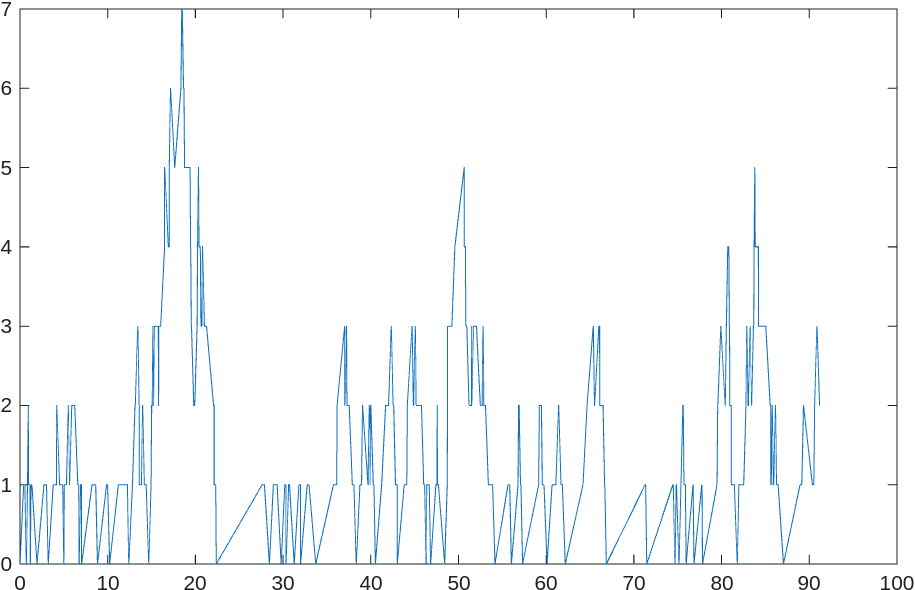
\includegraphics[width=7cm]{./images/samplePath.pdf}
  \caption{A sample path for a $M/E_2/1$ queueing station}
  \label{FIG:samplepath}
\end{figure}
\end{MATLAB}
\begin{JAVA}
\end{JAVA}
\begin{KOTLIN}
\end{KOTLIN}
\begin{PYTHON}
We may also plot the first 300 events as follows
\begin{lstlisting}[language = python]
# Plot first 300 events sample path
import matplotlib.pyplot as plt
plt.plot(sa.t[:300], sa.state[queue_index][:300])
plt.xlabel('Time')
plt.ylabel('Queue Length')
plt.title('Sample Path for M/E2/1 Queue')
plt.show()
\end{lstlisting}
\end{PYTHON}

We are now ready to filter the timestamps of events related to departures from the \texttt{queue} node
\begin{MATLAB}
\begin{lstlisting}[language = matlab]
ind = model.getNodeIndex(queue);
filtEvent = cellfun(@(c) c.node == ind && c.event == EventType.DEP, sa.event);
\end{lstlisting}
\end{MATLAB}
\begin{JAVA}
\begin{lstlisting}[language=java, basicstyle=\ttfamily\scriptsize]
// Filter events for departures from queue node
int queueIndex = model.getNodeIndex(queue);
boolean[] filtEvent = sa.filterEvents(queueIndex, EventType.DEP);
\end{lstlisting}
\end{JAVA}
\begin{KOTLIN}
\begin{lstlisting}[language=kotlin, basicstyle=\ttfamily\scriptsize]
// Filter events for departures from queue node
int queueIndex = model.getNodeIndex(queue);
boolean[] filtEvent = sa.filterEvents(queueIndex, EventType.DEP);
\end{lstlisting}
\end{KOTLIN}
\begin{PYTHON}
\begin{lstlisting}[language = python]
# Filter events for departures from queue node
queue_index = model.get_node_index(queue)
filt_event = sa.filter_events(queue_index, EventType.DEP)
\end{lstlisting}
\end{PYTHON}
Followed by a calculation of the time series of inter-departure times
\begin{MATLAB}
\begin{lstlisting}[language = matlab]
interDepTimes = diff(cellfun(@(c) c.t, {sa.event{filtEvent}}));
\end{lstlisting}
\end{MATLAB}
\begin{JAVA}
\begin{lstlisting}[language=java, basicstyle=\ttfamily\scriptsize]
// Calculate inter-departure times
double[] departureTimes = sa.getFilteredEventTimes(filtEvent);
double[] interDepTimes = new double[departureTimes.length - 1];
for (int i = 1; i < departureTimes.length; i++) {
    interDepTimes[i-1] = departureTimes[i] - departureTimes[i-1];
}
\end{lstlisting}
\end{JAVA}
\begin{KOTLIN}
\begin{lstlisting}[language=kotlin, basicstyle=\ttfamily\scriptsize]
// Calculate inter-departure times
double[] departureTimes = sa.getFilteredEventTimes(filtEvent);
double[] interDepTimes = new double[departureTimes.length - 1];
for (int i = 1; i < departureTimes.length; i++) {
    interDepTimes[i-1] = departureTimes[i] - departureTimes[i-1];
}
\end{lstlisting}
\end{KOTLIN}
\begin{PYTHON}
\begin{lstlisting}[language = python]
# Calculate inter-departure times (continued from above)
departure_times = [event.t for event, is_dep in zip(sa.event, filt_event) if is_dep]
inter_dep_times = np.diff(departure_times)
\end{lstlisting}
\end{PYTHON}
We may now for example compute the squared coefficient of variation of this process
\begin{MATLAB}
\begin{lstlisting}[language = matlab]
SCVdEst = var(interDepTimes)/mean(interDepTimes)^2
\end{lstlisting}
\end{MATLAB}
\begin{JAVA}
\begin{lstlisting}[language=java, basicstyle=\ttfamily\scriptsize]
// Calculate squared coefficient of variation
double mean = Arrays.stream(interDepTimes).average().orElse(0.0);
double variance = Arrays.stream(interDepTimes).map(x -> Math.pow(x - mean, 2)).average().orElse(0.0);
double SCVdEst = variance / (mean * mean);
System.out.println("SCV estimate: " + SCVdEst);
\end{lstlisting}
\end{JAVA}
\begin{KOTLIN}
\begin{lstlisting}[language=kotlin, basicstyle=\ttfamily\scriptsize]
// Calculate squared coefficient of variation
val mean = interDepTimes.average()
val variance = interDepTimes.map { (it - mean).pow(2) }.average()
val scvdEst = variance / (mean * mean)
println("SCV estimate: $scvdEst")
\end{lstlisting}
\end{KOTLIN}
\begin{PYTHON}
\begin{lstlisting}[language = python]
# Calculate squared coefficient of variation
scv_d_est = np.var(inter_dep_times) / np.mean(inter_dep_times)**2
print(f'SCV estimate: {scv_d_est}')
\end{lstlisting}
\end{PYTHON}
which evaluates to $0.8750$. Using Marshall's exact formula for the $GI/G/1$ queue~\cite{marshall1968some}, we get a theoretical value of $0.8750$. \Matlab{The calculation is included in the script associated to the example (\texttt{tut\_09\_dep\_process\_analysis.m}).}

\subsection{Tutorial 10: Basic layered queueing network}
\label{example-10-basic-layered-queueing-network}

This example demonstrates how to model and analyze a basic layered queueing network (LQN) representing a simple client-server application with two tiers: a client layer and a database layer.The LQN consists of a client processor P1 with a reference task T1 (10 users), a database processor P2 with an infinite server task T2, synchronous calls from the client to the database, exponential service times at both layers.

We start by creating the layered network instance:
\begin{MATLAB}
\begin{lstlisting}[language = matlab]
model = LayeredNetwork('ClientDBSystem');
\end{lstlisting}
\end{MATLAB}
\begin{JAVA}
\begin{lstlisting}[language = java, basicstyle=\ttfamily\scriptsize]
LayeredNetwork model = new LayeredNetwork("ClientDBSystem");
\end{lstlisting}
\end{JAVA}
\begin{KOTLIN}
\begin{lstlisting}[language = kotlin, basicstyle=\ttfamily\scriptsize]
val model = LayeredNetwork("ClientDBSystem")
\end{lstlisting}
\end{KOTLIN}
\begin{PYTHON}
\begin{lstlisting}[language = python]
model = LayeredNetwork('ClientDBSystem')
\end{lstlisting}
\end{PYTHON}

Next, we define the processors and tasks:
\begin{MATLAB}
\begin{lstlisting}[language = matlab]
% Create processors
P1 = Processor(model, 'ClientProcessor', 1, SchedStrategy.PS);
P2 = Processor(model, 'DBProcessor', 1, SchedStrategy.PS);

% Create tasks
T1 = Task(model, 'ClientTask', 10, SchedStrategy.REF).on(P1);
T1.setThinkTime(Exp.fitMean(5.0)); % 5-second think time
T2 = Task(model, 'DBTask', Inf, SchedStrategy.INF).on(P2);
\end{lstlisting}
\end{MATLAB}
\begin{JAVA}
\begin{lstlisting}[language = java, basicstyle=\ttfamily\scriptsize]
// Create processors
Processor P1 = new Processor(model, "ClientProcessor", 1, SchedStrategy.PS);
Processor P2 = new Processor(model, "DBProcessor", 1, SchedStrategy.PS);

// Create tasks
Task T1 = new Task(model, "ClientTask", 10, SchedStrategy.REF).on(P1);
T1.setThinkTime(Exp.fitMean(5.0)); // 5-second think time
Task T2 = new Task(model, "DBTask", Integer.MAX_VALUE, SchedStrategy.INF).on(P2);
\end{lstlisting}
\end{JAVA}
\begin{KOTLIN}
\begin{lstlisting}[language = kotlin, basicstyle=\ttfamily\scriptsize]
// Create processors
val P1 = Processor(model, "ClientProcessor", 1, SchedStrategy.PS)
val P2 = Processor(model, "DBProcessor", 1, SchedStrategy.PS)

// Create tasks
val T1 = Task(model, "ClientTask", 10, SchedStrategy.REF).on(P1)
T1.setThinkTime(Exp.fitMean(5.0)) // 5-second think time
val T2 = Task(model, "DBTask", Int.MAX_VALUE, SchedStrategy.INF).on(P2)
\end{lstlisting}
\end{KOTLIN}
\begin{PYTHON}
\begin{lstlisting}[language = python]
# Create processors
P1 = Processor(model, 'ClientProcessor', 1, SchedStrategy.PS)
P2 = Processor(model, 'DBProcessor', 1, SchedStrategy.PS)

# Create tasks
T1 = Task(model, 'ClientTask', 10, SchedStrategy.REF).on(P1)
T1.set_think_time(Exp.fit_mean(5.0))  # 5-second think time
T2 = Task(model, 'DBTask', float('inf'), SchedStrategy.INF).on(P2)
\end{lstlisting}
\end{PYTHON}

Now we define the entries that represent service interfaces:
\begin{MATLAB}
\begin{lstlisting}[language = matlab]
E1 = Entry(model, 'ClientEntry').on(T1);
E2 = Entry(model, 'DBEntry').on(T2);
\end{lstlisting}
\end{MATLAB}
\begin{JAVA}
\begin{lstlisting}[language = java, basicstyle=\ttfamily\scriptsize]
Entry E1 = new Entry(model, "ClientEntry").on(T1);
Entry E2 = new Entry(model, "DBEntry").on(T2);
\end{lstlisting}
\end{JAVA}
\begin{KOTLIN}
\begin{lstlisting}[language = kotlin, basicstyle=\ttfamily\scriptsize]
val E1 = Entry(model, "ClientEntry").on(T1)
val E2 = Entry(model, "DBEntry").on(T2)
\end{lstlisting}
\end{KOTLIN}
\begin{PYTHON}
\begin{lstlisting}[language = python]
E1 = Entry(model, 'ClientEntry').on(T1)
E2 = Entry(model, 'DBEntry').on(T2)
\end{lstlisting}
\end{PYTHON}

Finally, we define the activities that specify the service demand and the synchronous calls
\begin{MATLAB}
\begin{lstlisting}[language = matlab]
% Client activity: processes request and calls DB
A1 = Activity(model, 'ClientActivity', Exp.fitMean(1.0)).on(T1);
A1.bound_to(E1).synch_call(E2, 2.5); % 2.5 DB calls on average

% DB activity: processes database request
A2 = Activity(model, 'DBActivity', Exp.fitMean(0.8)).on(T2);
A2.bound_to(E2).replies_to(E2);
\end{lstlisting}
\end{MATLAB}
\begin{JAVA}
\begin{lstlisting}[language = java, basicstyle=\ttfamily\scriptsize]
// Client activity: processes request and calls DB
Activity A1 = new Activity(model, "ClientActivity", Exp.fitMean(1.0)).on(T1);
A1.boundTo(E1).synchCall(E2, 2.5); // 2.5 DB calls on average

// DB activity: processes database request
Activity A2 = new Activity(model, "DBActivity", Exp.fitMean(0.8)).on(T2);
A2.boundTo(E2).repliesTo(E2);
\end{lstlisting}
\end{JAVA}
\begin{KOTLIN}
\begin{lstlisting}[language = kotlin, basicstyle=\ttfamily\scriptsize]
// Client activity: processes request and calls DB
val A1 = Activity(model, "ClientActivity", Exp.fitMean(1.0)).on(T1)
A1.boundTo(E1).synchCall(E2, 2.5) // 2.5 DB calls on average

// DB activity: processes database request
val A2 = Activity(model, "DBActivity", Exp.fitMean(0.8)).on(T2)
A2.boundTo(E2).repliesTo(E2)
\end{lstlisting}
\end{KOTLIN}
\begin{PYTHON}
\begin{lstlisting}[language = python]
# Client activity: processes request and calls DB
A1 = Activity(model, 'ClientActivity', Exp.fit_mean(1.0)).on(T1)
A1.bound_to(E1).synch_call(E2, 2.5)  # 2.5 DB calls on average

# DB activity: processes database request
A2 = Activity(model, 'DBActivity', Exp.fit_mean(0.8)).on(T2)
A2.bound_to(E2).replies_to(E2)
\end{lstlisting}
\end{PYTHON}

Now we solve the layered network using the LN solver with MVA applied to each layer:
\begin{MATLAB}
\begin{lstlisting}[language = matlab]
solver = LN(model, @(m) MVA(m));
AvgTable = solver.avgTable();
AvgTable
\end{lstlisting}
The output shows the performance metrics for each node in the layered network:
\begin{lstlisting}[language = matlab, basicstyle=\ttfamily\scriptsize]
                 Node     NodeType     QLen      Util      RespT     ResidT    ArvR     Tput
    ____________________________________________________________________________________
    ClientProcessor      Processor      NaN    0.49913      NaN       NaN     NaN      NaN
    DBProcessor          Processor      NaN    0.99823      NaN       NaN     NaN      NaN
    ClientTask           RefTask        7.5    0.49913      NaN     1.7254    NaN    0.49913
    DBTask               Task         6.6433   0.99823      NaN      5.324    NaN     1.2478
    ClientEntry          Entry          7.5       NaN    15.035       NaN     NaN    0.49913
    DBEntry              Entry        6.6433      NaN     5.324       NaN     NaN     1.2478
    ClientActivity       Activity       7.5    0.49913    15.035    1.7254    NaN    0.49913
    DBActivity           Activity     6.6433   0.99823     5.324     5.324    NaN     1.2478
\end{lstlisting}
\end{MATLAB}
\begin{JAVA}
\begin{lstlisting}[language = java, basicstyle=\ttfamily\scriptsize]
SolverLN solver = new SolverLN(model, SolverType.MVA);
AvgTable avgTable = solver.avgTable();
avgTable.print();
\end{lstlisting}
\end{JAVA}
The output shows the performance metrics for each node in the layered network:
\begin{JAVA}
\begin{lstlisting}[language = java, basicstyle=\ttfamily\scriptsize]
Node      	NodeType  	QLen      	Util      	RespT     	ResidT    	ArvR      	Tput
ClientProcessor	Processor 	NaN       	0.49913   	NaN       	NaN       	NaN       	NaN
DBProcessor	Processor 	NaN       	0.99823   	NaN       	NaN       	NaN       	NaN
ClientTask	RefTask   	7.50000   	0.49913   	NaN       	1.72540   	NaN       	0.49913
DBTask    	Task      	6.64330   	0.99823   	NaN       	5.32400   	NaN       	1.24780
ClientEntry	Entry     	7.50000   	NaN       	15.03500  	NaN       	NaN       	0.49913
DBEntry   	Entry     	6.64330   	NaN       	5.32400   	NaN       	NaN       	1.24780
ClientActivity	Activity  	7.50000   	0.49913   	15.03500  	1.72540   	NaN       	0.49913
DBActivity	Activity  	6.64330   	0.99823   	5.32400   	5.32400   	NaN       	1.24780
\end{lstlisting}
\end{JAVA}
\begin{KOTLIN}
\begin{lstlisting}[language = kotlin, basicstyle=\ttfamily\scriptsize]
val solver = SolverLN(model, SolverType.MVA)
val avgTable = solver.avgTable()
avgTable.print()
\end{lstlisting}
The output shows the performance metrics for each node in the layered network:
\begin{lstlisting}[language = kotlin, basicstyle=\ttfamily\scriptsize]
Node      	NodeType  	QLen      	Util      	RespT     	ResidT    	ArvR      	Tput
ClientProcessor	Processor 	NaN       	0.49913   	NaN       	NaN       	NaN       	NaN
DBProcessor	Processor 	NaN       	0.99823   	NaN       	NaN       	NaN       	NaN
ClientTask	RefTask   	7.50000   	0.49913   	NaN       	1.72540   	NaN       	0.49913
DBTask    	Task      	6.64330   	0.99823   	NaN       	5.32400   	NaN       	1.24780
ClientEntry	Entry     	7.50000   	NaN       	15.03500  	NaN       	NaN       	0.49913
DBEntry   	Entry     	6.64330   	NaN       	5.32400   	NaN       	NaN       	1.24780
ClientActivity	Activity  	7.50000   	0.49913   	15.03500  	1.72540   	NaN       	0.49913
DBActivity	Activity  	6.64330   	0.99823   	5.32400   	5.32400   	NaN       	1.24780
\end{lstlisting}
\end{KOTLIN}
\begin{PYTHON}
\begin{lstlisting}[language = python]
solver = LN(model, lambda m: MVA(m))
avg_table = solver.avg_table()
print(avg_table)
\end{lstlisting}
The output shows the performance metrics for each node in the layered network:
\begin{lstlisting}[language = python, basicstyle=\ttfamily\scriptsize]
                 Node     NodeType     QLen      Util      RespT     ResidT    ArvR     Tput
ClientProcessor      Processor      NaN    0.4991       NaN       NaN     NaN      NaN
DBProcessor          Processor      NaN    0.9982       NaN       NaN     NaN      NaN
ClientTask           Task         7.5046   0.4991       NaN     1.7254    NaN    0.4991
DBTask               Task         6.6433   0.9982       NaN     5.3240    NaN    1.2478
ClientEntry          Entry        7.5046      NaN   15.0354       NaN     NaN    0.4991
DBEntry              Entry        6.6433      NaN    5.3240       NaN     NaN    1.2478
ClientActivity       Activity     7.5046   0.4991   15.0354    1.7254    NaN    0.4991
DBActivity           Activity     6.6433   0.9982    5.3240    5.3240    NaN    1.2478
\end{lstlisting}
\end{PYTHON}

\chapter{Network models}
\label{Network-models}

Throughout this chapter, we discuss the specification of \texttt{Network} models, which are extended queueing networks. \textsc{Line} currently supports open, closed, and mixed networks with non-exponential service and arrivals, and state-dependent routing\index{State-dependent routing|see{Network models}}. %Instead, we point to the following chapters for \texttt{CacheNetwork} and \texttt{LayeredNetwork} models.
All solvers support the computation of basic performance metrics, while some more advanced features are available only in specific solvers. %Tables are given later in the manual summarizing the features supported by each solver.
Each \texttt{Network} model requires in input a description of the nodes, the network topology, and the characteristics of the jobs that circulate within the network. In output, \textsc{Line} returns performance and reliability metrics.

The default metrics supported by all solvers are as follows:
\begin{itemize}
\item Mean queue-length (\texttt{QLen}). This is the mean number of jobs residing at a node when this is observed at a random instant of time.
\item Mean utilization (\texttt{Util}). For nodes that serve jobs, this is the mean fraction of time the node is busy processing jobs. In both single-server and multi-server nodes, this is a number normalized between 0 and 1, corresponding to 0\% and 100\%. In infinite-server nodes, the utilization is set by convention equal to the mean queue-length, therefore taking the interpretation of the mean number of jobs in execution at the station.
\item Mean response time (\texttt{RespT}). This is the mean time a job spends traversing a node within a network. If the node is visited multiple times, the response time is the time spent for a single visit to the node.
\item Mean residence time (\texttt{ResidT}). This is the total time a job accumulates, on average, to traverse a node within a network. If the node is visited multiple times, the residence time is the time accumulated overall visits to the node prior to returning to the reference station or arriving to a sink.
\item Mean throughput (\texttt{Tput}). This is the mean departure rate of jobs completed at a resource per time unit. Typically, this matches the mean arrival rate\index{Arrival Rate (ArvR)|see{Analysis methods}}, unless the node switches the class of the jobs in which case the arrival rate of a class may not match its departure rate.
\item Mean arrival rate (\texttt{ArvR}). This is the actual rate at which jobs of a given class arrive at a station, measured in jobs per unit time. The arrival rate differs from throughput primarily in networks with class-switching mechanisms, where jobs may arrive at a node in one class and depart in a different class. In such cases, the arrival rate for a class reflects the incoming flow before any class transformation occurs, while the throughput represents the outgoing flow after transformation. For nodes without class-switching, the arrival rate and throughput are identical under steady-state conditions due to flow balance. In open networks with probabilistic routing, the arrival rate at a downstream station depends on the throughput of upstream stations weighted by the routing probabilities. State-dependent routing strategies such as join-the-shortest-queue or round-robin introduce additional complexity, as the effective arrival rate at each destination varies dynamically based on system state. The arrival rate metric is particularly useful for validating Little's Law, which relates queue length, arrival rate, and response time, and for analyzing bottleneck behavior where high arrival rates relative to service capacity lead to queue buildup and increased delays.
\end{itemize}
The above metrics refer to the performance characteristics of individual nodes. Response times and throughputs can also be system-wide, meaning that they can describe end-to-end performance during the visit to the network. In this case, these metrics are called {\em system} metrics. System-level metrics include \texttt{SysRespT} (system response time), \texttt{SysTput} (system throughput), and \texttt{SysQLen} (system queue length). These system metrics aggregate information across all stations to provide a holistic view of network performance from the perspective of jobs as they complete their journey through the system. The system response time measures the total time a job spends in the network from entering at the source (for open classes) or leaving the reference station (for closed classes) until it exits at the sink or returns to complete at the reference station. The system throughput captures the rate at which jobs complete their end-to-end execution, accounting for all routing, queueing, and service delays encountered along their path. The system queue length represents the total number of jobs present anywhere in the network, summed across all stations and classes. These metrics can be retrieved using the \Matlab{\texttt{avgSys}}\Java{\texttt{avgSys}}\Kotlin{\texttt{avgSys}}\Python{\texttt{avg\_sys}} method, which returns system-level averages organized by chain rather than by individual station and class pairs. The corresponding \Matlab{\texttt{getAvgSys}}\Java{\texttt{getAvgSys}}\Kotlin{\texttt{getAvgSys}}\Python{\texttt{get\_avg\_sys}} function provides access to the same metrics in array format for programmatic manipulation. System-level metrics are particularly valuable when comparing alternative network configurations or evaluating the impact of parameter changes on overall system behavior, as they abstract away the details of individual station performance and focus on the end-to-end user experience.

\section{Network object definition}
\label{network-object-definition}
\subsection{Creating a network and its nodes}
A queueing network can be described in \textsc{Line} using the \texttt{Network} class constructor with a unique string identifying the model name:
\begin{MATLAB}
\begin{lstlisting}[language = matlab]
model = Network('myModel');
\end{lstlisting}
\end{MATLAB}
\begin{JAVA}
\begin{lstlisting}[language = java, basicstyle=\ttfamily\scriptsize]
Network model = new Network("myModel");
\end{lstlisting}
\end{JAVA}
\begin{KOTLIN}
\begin{lstlisting}[language = kotlin, basicstyle=\ttfamily\scriptsize]
val model: Network = Network("myModel")
\end{lstlisting}
\end{KOTLIN}
\begin{PYTHON}
\begin{lstlisting}[language = python]
model = Network('myModel')
\end{lstlisting}
\end{PYTHON}
The returned object of the \texttt{Network} class offers functions to instantiate and manage resource \emph{nodes} (stations,  delays, caches, ...) visited by jobs of several types (\emph{classes}).

A {node} is a resource in the network that can be visited by a job. A node must have a unique name and can either be {\em stateful} or {\em stateless}, the latter meaning that the node does not require state variables to determine its state or actions. If jobs visiting a stateful node can be required to spend time in it, the node is also said to be a {\em station}. A list of nodes available in \texttt{Network} models is given in Table~\ref{TAB_nodes}.

\begin{table}[t]
\renewcommand{\arraystretch}{1.2}
\centering
\caption{Nodes available in \texttt{Network} models.}
\begin{tabular}{|l|p{0.7\linewidth}|}
\hline
{Node} & {Description} \\
\hline
\texttt{Cache} & A node to switch job classes based on hits/misses in its cache\\
\texttt{ClassSwitch} & A node to switch job classes based on a static probability matrix\\
\texttt{Delay} & A station where jobs spend time without queueing\\
\texttt{Fork}\index{Fork|see{Network models}} & A node that forks jobs into tasks\\
\texttt{Join}\index{Join|see{Network models}} & A node that joins sibling tasks into the original job\\
\texttt{Logger} & A node that logs passage of jobs\\
\texttt{Queue} & A node where jobs queue and receive service\\
\texttt{Router} & A node that routes jobs to other nodes\\
\texttt{Sink} & Exit point for jobs in open classes\\
\texttt{Source} & Entry point for jobs in open classes\\
\hline
\end{tabular}
\label{TAB_nodes}
\end{table}

%For example, a sink is a stateless node, since its behaviour does not require state variables and jobs cannot sojourn in it. Instead, a first-come first-serve queue is a station, since jobs can sojourn inside its buffer and servers. A source is also treated in \textsc{Line} as a station since the inter-arrival time of jobs from the external world is considered as a time spent in the source, although this is not counted as part of the system response time.
%Lastly, a cache is a stateful node, since it needs to keep track of the cached items, however it is not a station since passage through this node occurs instantaneously.

We now provide more details on each of the nodes available in \texttt{Network} models.
\paragraph{Queue node.}
A \texttt{Queue} specifies a queueing station from its name and scheduling strategy, e.g.
\begin{MATLAB}
\begin{lstlisting}[language = matlab]
queue = Queue(model, 'Queue1', SchedStrategy.FCFS);
\end{lstlisting}
\end{MATLAB}
\begin{JAVA}
\begin{lstlisting}[language = java, basicstyle=\ttfamily\scriptsize]
Queue queue = new Queue(model, "Queue1", SchedStrategy.FCFS);
\end{lstlisting}
\end{JAVA}
\begin{KOTLIN}
\begin{lstlisting}[language = kotlin, basicstyle=\ttfamily\scriptsize]
val queue: Queue = Queue(model, "Queue1", SchedStrategy.FCFS)
\end{lstlisting}
\end{KOTLIN}
\begin{PYTHON}
\begin{lstlisting}[language=python]
queue = Queue(model, 'Queue1', SchedStrategy.FCFS)
\end{lstlisting}
\end{PYTHON}
specifies a first-come first-serve queue. It is alternatively possible to instantiate a queue using the \texttt{QueueingStation} constructor, which is merely an alias for \texttt{Queue}.

Queueing stations have by default a single server. The \Matlab{\texttt{setNumberOfServers}}\Java{\texttt{setNumberOfServers}}\Kotlin{\texttt{setNumberOfServers}}\Python{\texttt{set\_number\_of\_servers}} method can be used to instantiate multi-server stations. For heterogeneous servers with different capabilities, use \texttt{ServerType} to define server types and \texttt{HeteroSchedPolicy} to control which server types handle which job classes.

Valid scheduling strategies are specified within the \texttt{SchedStrategy} static class and include:
\begin{table}[ht!]
\renewcommand{\arraystretch}{1.2}
\centering
\caption{Scheduling strategies available in \textsc{Line}}
{\small
\begin{tabular}{|p{0.35\linewidth}|p{0.12\linewidth}|p{0.5\linewidth}|}
\hline
\textbf{Strategy} & \textbf{Code} & \textbf{Description} \\
\hline
First-come first-serve & \texttt{FCFS} & Jobs are served in order of arrival \\
\hline
Infinite-server\index{INF (Infinite Server)|see{Network models}} & \texttt{INF} & All jobs receive service simultaneously (delay station) \\
\hline
Processor-sharing & \texttt{PS} & Server capacity is shared equally among all present jobs \\
\hline
Service in random order & \texttt{SIRO} & Jobs are selected randomly for service \\
\hline
Discriminatory processor-sharing & \texttt{DPS} & Processor sharing with class-dependent weights \\
\hline
Generalized processor-sharing & \texttt{GPS} & Processor sharing with configurable weights per class \\
\hline
Shortest expected processing time & \texttt{SEPT} & Job with shortest expected processing time is served first \\
\hline
Shortest job first\index{SJF (Shortest Job First)|see{Network models}} & \texttt{SJF} & Job with shortest service requirement is served first \\
\hline
Polling & \texttt{POLLING} & Server cycles through queues in round-robin fashion \\
\hline
Last-come first-serve & \texttt{LCFS} & Most recently arrived job is served first \\
\hline
Least attained service\index{LAS (Least Attained Service)|see{Network models}} & \texttt{LAS} & Job with least accumulated service time gets priority \\
\hline
Earliest due date\index{EDD (Earliest Due Date)|see{Network models}} & \texttt{EDD} & Job with earliest deadline is served first \\
\hline
Limited processor sharing & \texttt{LPS} & Processor sharing with limit on concurrent jobs \\
\hline
Feedback scheduling & \texttt{FB} & Multi-level feedback scheduling \\
\hline
Longest expected processing time & \texttt{LEPT} & Job with longest expected processing time is served first \\
\hline
\end{tabular}}
\label{TAB_sched_strategies}
\end{table}
If a strategy requires class weights, these can be specified directly as an argument to the \Matlab{\texttt{setService}}\Java{\texttt{setService}}\Kotlin{\texttt{setService}}\Python{\texttt{set\_service}} function or using the \Matlab{\texttt{setStrategyParam}}\Java{\texttt{setStrategyParam}}\Kotlin{\texttt{setStrategyParam}}\Python{\texttt{set\_strategy\_param}} function, see later the description of DPS scheduling for an example.

\paragraph{Heterogeneous servers.}
Queue nodes can be configured with heterogeneous servers that have distinct service rates and job class compatibilities. This feature enables modeling of systems where servers have different capabilities or speeds, such as heterogeneous CPU pools, mixed-skill service desks, or tiered processing resources. The \texttt{ServerType} class allows defining server types within a queue, each with its own characteristics. To add a server type, first create a \texttt{ServerType} object with a name and the number of servers of that type, then pass it to the \Matlab{\texttt{addServerType}}\Java{\texttt{addServerType}}\Kotlin{\texttt{addServerType}}\Python{\texttt{add\_server\_type}} method. After creating server types, configure their service rates per job class using the same methods as for homogeneous queues, but targeting specific server types. Optionally, the scheduling policy for heterogeneous servers can be controlled using \texttt{HeteroSchedPolicy}, which determines how jobs are assigned to available server types. This allows specifying whether jobs can only be served by compatible server types or whether more sophisticated assignment policies are used. The following example demonstrates a queue with two server types, fast and slow servers, where each type has different service rates.
\begin{MATLAB}
\begin{lstlisting}[language = matlab]
queue = Queue(model, 'HeteroQueue', SchedStrategy.FCFS);
fastType = ServerType('FastServer', 2);
slowType = ServerType('SlowServer', 2);
queue.addServerType(fastType);
queue.addServerType(slowType);
queue.setService(jobclass, Exp(1.0), fastType);
queue.setService(jobclass, Exp(0.5), slowType);
\end{lstlisting}
\end{MATLAB}
\begin{JAVA}
\begin{lstlisting}[language = java, basicstyle=\ttfamily\scriptsize]
Queue queue = new Queue(model, "HeteroQueue", SchedStrategy.FCFS);
ServerType fastType = new ServerType("FastServer", 2);
ServerType slowType = new ServerType("SlowServer", 2);
queue.addServerType(fastType);
queue.addServerType(slowType);
queue.setService(jobclass, new Exp(1.0), fastType);
queue.setService(jobclass, new Exp(0.5), slowType);
\end{lstlisting}
\end{JAVA}
\begin{KOTLIN}
\begin{lstlisting}[language = kotlin, basicstyle=\ttfamily\scriptsize]
val queue = Queue(model, "HeteroQueue", SchedStrategy.FCFS)
val fastType = ServerType("FastServer", 2)
val slowType = ServerType("SlowServer", 2)
queue.addServerType(fastType)
queue.addServerType(slowType)
queue.setService(jobclass, Exp(1.0), fastType)
queue.setService(jobclass, Exp(0.5), slowType)
\end{lstlisting}
\end{KOTLIN}
\begin{PYTHON}
\begin{lstlisting}[language = python]
queue = Queue(model, 'HeteroQueue', SchedStrategy.FCFS)
fast_type = ServerType('FastServer', 2)
slow_type = ServerType('SlowServer', 2)
queue.add_server_type(fast_type)
queue.add_server_type(slow_type)
queue.set_service(jobclass, Exp(1.0), fast_type)
queue.set_service(jobclass, Exp(0.5), slow_type)
\end{lstlisting}
\end{PYTHON}
This capability is particularly useful for capacity planning studies where resource pools contain servers with varying performance characteristics, or for modeling systems where specialization or skill matching affects service delivery.

When a job is compatible with multiple server types, the \texttt{HeteroSchedPolicy} class determines the assignment strategy. The available policies are listed in Table~\ref{tab:heteroschedpolicy}.
\begin{table}[ht!]
\renewcommand{\arraystretch}{1.2}
\centering
\caption{Heterogeneous server assignment policies (\texttt{HeteroSchedPolicy})}
\label{tab:heteroschedpolicy}
{\small
\begin{tabular}{|p{0.18\linewidth}|p{0.78\linewidth}|}
\hline
\textbf{Policy} & \textbf{Description} \\
\hline
\texttt{ORDER} & Assign to the first compatible server type in definition order (default) \\
\hline
\texttt{ALIS} & Assign Longest Idle Server: routes to the server type with the longest accumulated idle time (round-robin with busy servers placed at the back of the priority list) \\
\hline
\texttt{ALFS} & Assign Longest Free Server: similar to ALIS but with a fairness-based sorting that accounts for server coverage across job classes \\
\hline
\texttt{FAIRNESS} & Distributes jobs fairly across all compatible server types, balancing load proportional to the number of servers of each type \\
\hline
\texttt{FSF} & Fastest Server First: assigns the job to the compatible server type with the minimum expected service time \\
\hline
\texttt{RAIS} & Random Available Idle Server: selects uniformly at random among compatible server types that have at least one idle server \\
\hline
\end{tabular}}
\end{table}
The policy is set via \Matlab{\texttt{queue.setHeteroSchedPolicy(HeteroSchedPolicy.FSF)}}\Java{\texttt{queue.setHeteroSchedPolicy(HeteroSchedPolicy.FSF)}}\Kotlin{\texttt{queue.setHeteroSchedPolicy(HeteroSchedPolicy.FSF)}}\Python{\texttt{queue.set\_hetero\_sched\_policy(HeteroSchedPolicy.FSF)}}.

\paragraph{Delay node.} Delay stations, also called infinite server stations, may be instantiated either as objects of \texttt{Queue} class, with the \texttt{SchedStrategy.INF} scheduling strategy, or using the following specialized constructor
\begin{MATLAB}
\begin{lstlisting}[language = matlab]
delay = Delay(model, 'ThinkTime');
\end{lstlisting}
\end{MATLAB}
\begin{JAVA}
\begin{lstlisting}[language = java, basicstyle=\ttfamily\scriptsize]
Delay delay = new Delay(model, "ThinkTime");
\end{lstlisting}
\end{JAVA}
\begin{KOTLIN}
\begin{lstlisting}[language = kotlin, basicstyle=\ttfamily\scriptsize]
val delay: Delay = Delay(model, "ThinkTime")
\end{lstlisting}
\end{KOTLIN}
\begin{PYTHON}
\begin{lstlisting}[language = python]
delay = Delay(model, 'ThinkTime')
\end{lstlisting}
\end{PYTHON}

As for queues, for readability it is possible to instantiate delay nodes using the \texttt{DelayStation} class which is an alias for the \texttt{Delay} class.

\paragraph{Source and Sink nodes.} As seen in the M/M/1 getting started example, these nodes are mandatory elements for the specification of open classes. Their constructor only requires a specification of the unique name associated to the nodes:
\begin{MATLAB}
\begin{lstlisting}[language = matlab]
source = Source(model, 'Source');
sink = Sink(model, 'Sink');
\end{lstlisting}
\end{MATLAB}
\begin{JAVA}
\begin{lstlisting}[language = java, basicstyle=\ttfamily\scriptsize]
Source source = new Source(model, "Source");
Sink sink = new Sink(model, "Sink");
\end{lstlisting}
\end{JAVA}
\begin{KOTLIN}
\begin{lstlisting}[language = kotlin, basicstyle=\ttfamily\scriptsize]
val source: Source = Source(model, "Source")
val sink: Sink = Sink(model, "Sink")
\end{lstlisting}
\end{KOTLIN}
\begin{PYTHON}
\begin{lstlisting}[language = python]
source = Source(model, 'Source')
sink = Sink(model, 'Sink')
\end{lstlisting}
\end{PYTHON}

The \texttt{Source} node supports state-dependent arrival rates via the load-dependent scaling mechanism. Instead of specifying a fixed inter-arrival distribution, the effective arrival rate can vary as a function of the total number of jobs in the system. This is achieved by assigning a load-dependent rate function to the Source station using the \texttt{lldscaling} mechanism, in the same way load-dependent service rates are specified for queue nodes (see the load-dependent service section under Advanced node parameters). When a load-dependent arrival rate is defined, the \texttt{CTMC} and \texttt{SSA} solvers automatically account for state-dependent rates during analysis, enabling accurate modeling of systems where arrival rates diminish as congestion increases (e.g., finite source populations or flow-controlled networks).

\paragraph{Customer impatience and reneging.}
Queue nodes support customer impatience, where jobs may abandon the queue if their waiting time becomes excessive. This feature models real-world scenarios such as call centers where customers hang up after waiting too long, web users navigating away from slow-loading pages, or service systems where customers leave due to long queues. The \Matlab{\texttt{setPatience}}\Java{\texttt{setPatience}}\Kotlin{\texttt{setPatience}}\Python{\texttt{set\_patience}} method on Queue nodes specifies a patience distribution for a given job class. When a job arrives or begins waiting, a patience time is sampled from this distribution. If the job's waiting time exceeds this sampled patience time before service begins, the job abandons the queue and exits the system. The patience distribution can be any standard distribution supported by \textsc{Line}, such as exponential for memoryless impatience or deterministic for fixed deadlines. The following example demonstrates a queue where jobs of a certain class have exponentially distributed patience with mean 10 time units.
\begin{MATLAB}
\begin{lstlisting}[language = matlab]
queue = Queue(model, 'ServiceQueue', SchedStrategy.FCFS);
queue.setPatience(jobclass, Exp(0.1)); % mean patience = 10
\end{lstlisting}
\end{MATLAB}
\begin{JAVA}
\begin{lstlisting}[language = java, basicstyle=\ttfamily\scriptsize]
Queue queue = new Queue(model, "ServiceQueue", SchedStrategy.FCFS);
queue.setPatience(jobclass, new Exp(0.1)); // mean patience = 10
\end{lstlisting}
\end{JAVA}
\begin{KOTLIN}
\begin{lstlisting}[language = kotlin, basicstyle=\ttfamily\scriptsize]
val queue = Queue(model, "ServiceQueue", SchedStrategy.FCFS)
queue.setPatience(jobclass, Exp(0.1)) // mean patience = 10
\end{lstlisting}
\end{KOTLIN}
\begin{PYTHON}
\begin{lstlisting}[language = python]
queue = Queue(model, 'ServiceQueue', SchedStrategy.FCFS)
queue.set_patience(jobclass, Exp(0.1))  # mean patience = 10
\end{lstlisting}
\end{PYTHON}
This feature is primarily supported by the JMT solver through discrete event simulation, which can accurately track individual job patience times and trigger abandonment events. Customer impatience is particularly relevant for performance analysis of systems with quality-of-service constraints, where understanding abandonment rates and their impact on effective throughput is critical for capacity planning and service level agreement compliance.

\paragraph{Fork and Join nodes.} The fork\index{fork-join systems (parallel processing models)|see{Network models}}\index{Fork-join systems|see{Network models}} and join nodes are currently available only for the \texttt{JMT} solver. The \texttt{Fork} splits an incoming job into a set of sibling tasks, sending out one task for each outgoing link. These tasks inherit the class of the original job and are served as normal jobs until they are reassembled at a \texttt{Join} station.

Their specification of Fork and Join nodes only requires the name of the node
\begin{MATLAB}
\begin{lstlisting}[language = matlab]
fork = Fork(model, 'Fork');
join = Join(model, 'Join', fork);
\end{lstlisting}
\end{MATLAB}
\begin{JAVA}
\begin{lstlisting}[language = java, basicstyle=\ttfamily\scriptsize]
Fork fork = new Fork(model, "Fork");
Join join = new Join(model, "Join", fork);
\end{lstlisting}
\end{JAVA}
\begin{KOTLIN}
\begin{lstlisting}[language = kotlin, basicstyle=\ttfamily\scriptsize]
val fork: Fork = Fork(model, "Fork")
val join: Join = Join(model, "Join", fork)
\end{lstlisting}
\end{KOTLIN}
\begin{PYTHON}
\begin{lstlisting}[language = python]
fork = Fork(model, 'Fork')
join = Join(model, 'Join', fork)
\end{lstlisting}
\end{PYTHON}

The number of tasks sent by a \texttt{Fork} on each output link can be set using the \Matlab{\texttt{setTasksPerLink}}\Java{\texttt{setTasksPerLink}}\Kotlin{\texttt{setTasksPerLink}}\Python{\texttt{set\_tasks\_per\_link}} method of the \texttt{fork} object. To enable effective analytical approximations, presently \textsc{Line} requires that every join node is bound to a specific fork node, although specific solvers will ignore this information (e.g., \textsc{JMT}).

Also note that the routing probabilities out of the \texttt{Fork} node need to be set to 1.0 towards every other node connected to the \texttt{Fork}. For example, a \texttt{Fork} sending jobs in class 1 to nodes $A$, $B$ and $C$, cannot send jobs in class $2$ only to $A$ and $B$: it must send them to all three connected nodes $A$, $B$ and $C$. A new fork node visited only by class-2 jobs needs to be created in order to send that class of jobs only to $A$ and $B$.

Fork nodes also support probabilistic (state-dependent) branching via \texttt{RoutingStrategy.PROB}, where different output links carry non-uniform routing probabilities. This is set using \Matlab{\texttt{setProbRouting}}\Java{\texttt{setProbRouting}}\Kotlin{\texttt{setProbRouting}}\Python{\texttt{set\_prob\_routing}} on the Fork node and is available when using \texttt{JMT}. This allows a Fork node to direct tasks to different parallel branches with configurable proportions, enabling asymmetric fork-join models where not all branches are equally loaded.

After splitting a job into tasks, \textsc{Line} takes the convention that visit counts refer to the average number of passages at the target resources for the original job, scaled by the number of tasks. For example, if a job is split into two tasks at a fork node, each visiting respectively nodes $A$ and $B$, the average visit count at $A$ and $B$ will be 0.5.

For Fork-Join response time percentiles, \texttt{SolverMAM} automatically detects valid FJ topologies (Source $\rightarrow$ Fork $\rightarrow$ K Queues $\rightarrow$ Join $\rightarrow$ Sink) and applies percentile computation as follows %Supported distributions include Exp, HyperExp(2), Erlang(2), and MAP(2). Options \texttt{fj\_accuracy} (default: 100) and \texttt{fj\_tmode} (\texttt{'NARE'} or \texttt{'Sylves'}) control the approximation.
\begin{MATLAB}
\begin{lstlisting}[language = matlab]
solver = SolverMAM(model);
[percRT, percTable] = solver.getPerctRespT([90, 95, 99]);
\end{lstlisting}
\end{MATLAB}
\begin{JAVA}
\begin{lstlisting}[language = java, basicstyle=\ttfamily\scriptsize]
SolverMAM solver = new SolverMAM(model);
Matrix percRT = solver.getPerctRespT(new double[]{90, 95, 99});
\end{lstlisting}
\end{JAVA}
\begin{KOTLIN}
\begin{lstlisting}[language = kotlin, basicstyle=\ttfamily\scriptsize]
val solver = SolverMAM(model)
val percRT = solver.getPerctRespT(doubleArrayOf(90.0, 95.0, 99.0))
\end{lstlisting}
\end{KOTLIN}
\begin{PYTHON}
\begin{lstlisting}[language = python]
solver = SolverMAM(model)
perc_rt = solver.get_perct_resp_t([90, 95, 99])
\end{lstlisting}
\end{PYTHON}

\paragraph{ClassSwitch node.} This is a stateless node to change the class of a transiting job based on a static probabilistic policy. For example, it is possible to specify that all jobs belonging to class 1 should become of class 2 with probability $1.0$, or that a transiting job of class 2 should become of class 1 with probability $0.3$. This example is instantiated as follows
\begin{MATLAB}
\begin{lstlisting}[language = matlab]
cs = ClassSwitch(model, 'ClassSwitchPoint',[0.0, 1.0; 0.3, 0.7]);
\end{lstlisting}
\end{MATLAB}
\begin{JAVA}
\begin{lstlisting}[language = java, basicstyle=\ttfamily\scriptsize]
ClassSwitch cs = new ClassSwitch(model,"ClassSwitchPoint", new Matrix("[0.0, 1.0; 0.3, 0.7]"));
\end{lstlisting}
Note that the argument of the \texttt{Matrix} constructor is a string specifying a matrix in MATLAB format, i,e., where the semi-colon separates rows. Alternatively, it is also possible to use Python format, e.g.,
\begin{lstlisting}[language = java, basicstyle=\ttfamily\scriptsize]
ClassSwitch cs = new ClassSwitch(model,"ClassSwitchPoint", new Matrix("[[0.0, 1.0], [0.3, 0.7]]"));
\end{lstlisting}
\end{JAVA}
\begin{KOTLIN}
\begin{lstlisting}[language = kotlin, basicstyle=\ttfamily\scriptsize]
val cs: ClassSwitch = ClassSwitch(model,"ClassSwitchPoint", Matrix("[0.0, 1.0; 0.3, 0.7]"))
\end{lstlisting}
Note that the argument of the \texttt{Matrix} constructor is a string specifying a matrix in MATLAB format, i,e., where the semi-colon separates rows. Alternatively, it is also possible to use Python format, e.g.,
\begin{lstlisting}[language = kotlin, basicstyle=\ttfamily\scriptsize]
val cs: ClassSwitch = ClassSwitch(model,"ClassSwitchPoint", Matrix("[[0.0, 1.0], [0.3, 0.7]]"))
\end{lstlisting}
\end{KOTLIN}
\begin{PYTHON}
\begin{lstlisting}[language = python]
cs = ClassSwitch(model, 'ClassSwitchPoint', [[0.0, 1.0], [0.3, 0.7]])
\end{lstlisting}
\end{PYTHON}


\paragraph{Cache node.} This is a stateful node to store one or more items in a cache of finite size, for which it is possible to specify a replacement policy.  The {\em cache} constructor requires the total cache capacity and the number of items that can be referenced by the jobs in transit, e.g.,
\begin{MATLAB}
\begin{lstlisting}[language = matlab]
cacheNode = Cache(model, 'Cache1', nitems, capacity, ReplacementStrategy.LRU);
\end{lstlisting}
\end{MATLAB}
\begin{JAVA}
\begin{lstlisting}[language = java, basicstyle=\ttfamily\scriptsize]
Cache cacheNode = new Cache(model, "Cache1", nitems, capacity, ReplacementStrategy.LRU);
\end{lstlisting}
\end{JAVA}
\begin{KOTLIN}
\begin{lstlisting}[language = kotlin, basicstyle=\ttfamily\scriptsize]
val cacheNode: Cache = Cache(model, "Cache1", nitems, capacity, ReplacementStrategy.LRU)
\end{lstlisting}
\end{KOTLIN}
\begin{PYTHON}
\begin{lstlisting}[language = python]
cacheNode = Cache(model, 'Cache1', nitems, capacity, ReplacementStrategy.LRU)
\end{lstlisting}
\end{PYTHON}

If the capacity is a scalar integer (e.g., \texttt{15}), then it represents the total number of items that can be cached and the value cannot be greater than the number of items. Conversely, if it is a vector of integers (e.g., \Matlab{\texttt{[10,5]}}\Java{Matrix("[10,5]")}\Kotlin{Matrix("[10,5]")}\Python{[10,5]}) then the node is a list-based cache, where the vector entries specify the capacity of each list. We point to \cite{GastH16} for more details on list-based caches and their replacement policies.

Available replacement policies are specified within the \texttt{ReplacementStrategy} static class and include:
\begin{itemize}
\item First-in first-out (\texttt{ReplacementStrategy.FIFO})
\item Random replacement (\texttt{ReplacementStrategy.RR})
\item Least-recently used (\texttt{ReplacementStrategy.LRU})
\item Strict first-in first-out (\texttt{ReplacementStrategy.SFIFO})
\end{itemize}
Upon cache hit or cache miss, a job in transit is switched to a user-specified class. More details are given later in Section~\ref{class-switching}.

Beyond basic capacity constraints, cache nodes in \textsc{Line} support weight-based occupancy policies where each cached item can consume a configurable amount of storage space rather than occupying a single slot. This is useful for modeling caches where objects have heterogeneous sizes, such as web caches storing documents of varying lengths. The FCRWeight and FCRMemOcc mechanisms enable specification of per-item weights counted against the total cache capacity. State-dependent routing exploits detailed cache state information to direct jobs along different paths depending on whether their requested item is present in the cache. When a job requests a cached item (a hit), it is classified into a hit class and routed to a delay node representing fast cache access, while jobs experiencing misses are switched to a miss class and directed to a queue representing slower backend retrieval. Solvers such as CTMC and NC employ stochastic complementation techniques to efficiently analyze cache models by eliminating intermediate Router states and computing effective transition rates between observable cache states.

\paragraph{Router node.} This node is able to route jobs according to a specified \texttt{RoutingStrategy}, which can either be probabilistic or not (e.g., round-robin). Upon entering a \texttt{Router}, a job neither waits nor receives service; it is instead directly forwarded to the next node according to the specified routing strategy. A \texttt{Router} can be instantiated as follows:
\begin{MATLAB}
\begin{lstlisting}[language = matlab]
router = Router(model, 'RouterNode');
\end{lstlisting}
\end{MATLAB}
\begin{JAVA}
\begin{lstlisting}[language = java, basicstyle=\ttfamily\scriptsize]
Router router = new Router(model, "RouterNode");
\end{lstlisting}
\end{JAVA}
\begin{KOTLIN}
\begin{lstlisting}[language = kotlin, basicstyle=\ttfamily\scriptsize]
val router: Router = Router(model, "RouterNode")
\end{lstlisting}
\end{KOTLIN}
\begin{PYTHON}
\begin{lstlisting}[language = python]
router = Router(model, 'RouterNode')
\end{lstlisting}
\end{PYTHON}
An example of use of this node is given in Section~\ref{example-4-round-robin-load-balancing}. Routing strategies need to be specified for each class using the \Matlab{\texttt{setRouting}}\Java{\texttt{setRouting}}\Kotlin{\texttt{setRouting}}\Python{\texttt{set\_routing}} method and valid choices are as follows
\begin{itemize}
\item Random routing (\texttt{RoutingStrategy.RAND})
\item Round robin (\texttt{RoutingStrategy.RROBIN})
\item Probabilistic routing (\texttt{RoutingStrategy.PROB})
\item Join-the-shortest-queue (\texttt{RoutingStrategy.JSQ})
\end{itemize}
For example, assume that \texttt{oclass} is a class of jobs. In order to route jobs in this class with equal probabilities to every outgoing link we set
\begin{MATLAB}
\begin{lstlisting}[language = matlab]
router.setRouting(oclass, RoutingStrategy.RAND);
\end{lstlisting}
\end{MATLAB}
\begin{JAVA}
\begin{lstlisting}[language = java, basicstyle=\ttfamily\scriptsize]
router.setRouting(oclass, RoutingStrategy.RAND);
\end{lstlisting}
\end{JAVA}
\begin{KOTLIN}
\begin{lstlisting}[language = kotlin, basicstyle=\ttfamily\scriptsize]
router.setRouting(oclass, RoutingStrategy.RAND)
\end{lstlisting}
\end{KOTLIN}
\begin{PYTHON}
\begin{lstlisting}[language = python]
router.set_routing(oclass, RoutingStrategy.RAND)
\end{lstlisting}
\end{PYTHON}
It should be noted that \Matlab{\texttt{setRouting}}\Java{\texttt{setRouting}}\Kotlin{\texttt{setRouting}}\Python{\texttt{set\_routing}} is also available for all other nodes such as queueing stations, delays, etc. Therefore, the added value of the \texttt{Router} node is the ability to represent certain system elements that centralize the routing logic, such as load balancers.

\paragraph{Logger node.} A logger node is a node that closely resembles the logger node available in the JSIMgraph simulator within JMT. At present, models that include this element can only be solved using the \texttt{JMT} solver.

A \texttt{Logger} node records information about passing jobs in a \texttt{csv} file, such as the timestamp of passage and general information about the jobs. The node can be instantiated as follows
\begin{MATLAB}
\begin{lstlisting}[language = matlab]
logger=Logger(model,'LoggerNode','logfile.csv');
\end{lstlisting}
\end{MATLAB}
\begin{JAVA}
\begin{lstlisting}[language=java, basicstyle=\ttfamily\scriptsize]
Logger logger = new Logger(model, "LoggerNode", "logfile.csv");
\end{lstlisting}
\end{JAVA}
\begin{KOTLIN}
\begin{lstlisting}[language=kotlin, basicstyle=\ttfamily\scriptsize]
val logger = Logger(model, "LoggerNode", "logfile.csv")
\end{lstlisting}
\end{KOTLIN}
\begin{PYTHON}
\begin{lstlisting}[language=python]
logger = Logger(model, 'LoggerNode', 'logfile.csv')
\end{lstlisting}
\end{PYTHON}

The Logger node provides fine-grained control over what information is captured for each job passage through configuration properties. Event logging can be customized to include the simulation start time, the logger node name, the current timestamp when the job passes through, the unique job identifier, the job class, the time since the last job of the same class passed through, and the time since any job of any class last passed. These boolean configuration options allow selective recording based on analysis requirements, reducing log file size when only specific metrics are needed. The CSV output format writes one row per job passage with columns corresponding to the enabled logging options. Departure timestamp recording captures the exact simulation time when jobs leave the logger, enabling post-analysis of inter-arrival time distributions, service time variability, and queueing delays at different points in the network. The LogTunnel section that implements the logging behavior operates transparently without introducing queueing delay, ensuring that logger placement does not alter the performance characteristics being measured. Jobs pass through the logger instantaneously while their passage event is recorded, making loggers suitable for placement at any point in the network topology without affecting throughput or response time metrics. When multiple loggers are placed at different network locations, their combined output provides a detailed trace of job trajectories through the system, supporting visualization of flow patterns and identification of bottlenecks. The logger output can be post-processed to compute empirical distributions, perform statistical hypothesis tests comparing different model configurations, or validate simulation results against analytical solver predictions.

The following methods can be used to specify the information that needs to be stored in the \texttt{csv} file
\begin{itemize}
\item \Matlab{\texttt{setStartTime}}\Java{\texttt{setStartTime}}\Kotlin{\texttt{setStartTime}}\Python{\texttt{set\_start\_time}}: record a timestamp for the wallclock time when the simulation started.
\item \Matlab{\texttt{setJobID}}\Java{\texttt{setJobID}}\Kotlin{\texttt{setJobID}}\Python{\texttt{set\_job\_id}}: record a unique id for the passing job.
\item \Matlab{\texttt{setJobClass}}\Java{\texttt{setJobClass}}\Kotlin{\texttt{setJobClass}}\Python{\texttt{set\_job\_class}}: record the class of the passing job.
\item \Matlab{\texttt{setTimestamp}}\Java{\texttt{setTimestamp}}\Kotlin{\texttt{setTimestamp}}\Python{\texttt{set\_timestamp}}: record a timestamp for the simulated time when the job passed in the logger.
\item \Matlab{\texttt{setTimeSameClass}}\Java{\texttt{setTimeSameClass}}\Kotlin{\texttt{setTimeSameClass}}\Python{\texttt{set\_time\_same\_class}}: record the time elapsed since the last passage of a job of the same class.
\item \Matlab{\texttt{setTimeAnyClass}}\Java{\texttt{setTimeAnyClass}}\Kotlin{\texttt{setTimeAnyClass}}\Python{\texttt{set\_time\_any\_class}}: record the time elapsed since the last passage of a job of any class.
\end{itemize}
Each method can be called either with a single \Matlab{\texttt{true} or \texttt{false}}\Java{\texttt{true} or \texttt{false}}\Kotlin{\texttt{true} or \texttt{false}}\Python{\texttt{True} or \texttt{False}} argument, to enable or disable the recording of the corresponding information, e.g.
\begin{MATLAB}
\begin{lstlisting}[language = matlab]
logger.setJobClass(true);
\end{lstlisting}
\end{MATLAB}
\begin{JAVA}
\begin{lstlisting}[language=java, basicstyle=\ttfamily\scriptsize]
logger.setJobClass(true);
\end{lstlisting}
\end{JAVA}
\begin{KOTLIN}
\begin{lstlisting}[language=kotlin, basicstyle=\ttfamily\scriptsize]
logger.setJobClass(true)
\end{lstlisting}
\end{KOTLIN}
\begin{PYTHON}
\begin{lstlisting}[language=python]
logger.set_job_class(True)
\end{lstlisting}
\end{PYTHON}
The routing behavior of jobs can be set up as explained for regular nodes such as queues or delay stations.

\paragraph{Place and Transition nodes.} \textsc{Line} supports stochastic Petri net modeling via \texttt{Place} and \texttt{Transition} nodes. A \texttt{Place} holds tokens representing jobs or resources, while a \texttt{Transition} fires when its enabling conditions are met, consuming tokens from input places and producing tokens at output places. Transitions support multiple firing modes, each with its own enabling/inhibiting conditions, firing priorities, and firing rate distributions. Modes allow a single transition to represent different behaviors depending on system state. For example:
\begin{MATLAB}
\begin{lstlisting}[language = matlab]
place = Place(model, 'Buffer');
trans = Transition(model, 'Process');
fastMode = trans.addMode('fast');  % returns Mode object
slowMode = trans.addMode('slow');
trans.setDistribution(fastMode, Exp(2.0));  % fast processing mode
trans.setDistribution(slowMode, Exp(0.5));  % slow processing mode
trans.setEnablingConditions(fastMode, jobclass, place, 1);  % requires 1 token
trans.setEnablingConditions(slowMode, jobclass, place, 1);
\end{lstlisting}
\end{MATLAB}
\begin{JAVA}
\begin{lstlisting}[language = java, basicstyle=\ttfamily\scriptsize]
Place place = new Place(model, "Buffer");
Transition trans = new Transition(model, "Process");
Mode fastMode = trans.addMode("fast");  // returns Mode object
Mode slowMode = trans.addMode("slow");
trans.setDistribution(fastMode, new Exp(2.0));  // fast processing mode
trans.setDistribution(slowMode, new Exp(0.5));  // slow processing mode
trans.setEnablingConditions(fastMode, jobclass, place, 1);  // requires 1 token
trans.setEnablingConditions(slowMode, jobclass, place, 1);
\end{lstlisting}
\end{JAVA}
\begin{KOTLIN}
\begin{lstlisting}[language = kotlin, basicstyle=\ttfamily\scriptsize]
val place = Place(model, "Buffer")
val trans = Transition(model, "Process")
val fastMode = trans.addMode("fast")  // returns Mode object
val slowMode = trans.addMode("slow")
trans.setDistribution(fastMode, Exp(2.0))  // fast processing mode
trans.setDistribution(slowMode, Exp(0.5))  // slow processing mode
trans.setEnablingConditions(fastMode, jobclass, place, 1)  // requires 1 token
trans.setEnablingConditions(slowMode, jobclass, place, 1)
\end{lstlisting}
\end{KOTLIN}
\begin{PYTHON}
\begin{lstlisting}[language = python]
place = Place(model, 'Buffer')
trans = Transition(model, 'Process')
fast_mode = trans.add_mode('fast')  # returns Mode object
slow_mode = trans.add_mode('slow')
trans.set_distribution(fast_mode, Exp(2.0))  # fast processing mode
trans.set_distribution(slow_mode, Exp(0.5))  # slow processing mode
trans.set_enabling_conditions(fast_mode, jobclass, place, 1)  # requires 1 token
trans.set_enabling_conditions(slow_mode, jobclass, place, 1)
\end{lstlisting}
\end{PYTHON}
Examples are provided in \texttt{spn\_basic\_open}, \texttt{spn\_twomodes}, and related files in the \texttt{examples/} folder.

\subsection{Advanced node parameters}
\label{advanced-node-parameters}

\subsubsection{Scheduling parameters}
\label{scheduling-parameters}
Upon setting service distributions at a station, one may also specify scheduling parameters such as weights as additional arguments to the \Matlab{\texttt{setService}}\Java{\texttt{setService}}\Kotlin{\texttt{setService}}\Python{\texttt{set\_service}} function. For example, if the node implements discriminatory processor sharing (\texttt{SchedStrategy.DPS}), the command
\begin{MATLAB}
\begin{lstlisting}[language = matlab]
queue.setService(class2, Cox2.fitMeanAndSCV(0.2,10), 5.0);
\end{lstlisting}
\end{MATLAB}
\begin{JAVA}
\begin{lstlisting}[language = java, basicstyle=\ttfamily\scriptsize]
queue.setService(class2, Cox2.fitMeanAndSCV(0.2,10.0), 5.0);
\end{lstlisting}
\end{JAVA}
\begin{KOTLIN}
\begin{lstlisting}[language = kotlin, basicstyle=\ttfamily\scriptsize]
queue.setService(class2, Cox2.fitMeanAndSCV(0.2,10.0), 5.0)
\end{lstlisting}
\end{KOTLIN}
\begin{PYTHON}
\begin{lstlisting}[language = python]
queue.set_service(class2, Cox2.fit_mean_and_scv(0.2,10), 5.0)
\end{lstlisting}
\end{PYTHON}
assigns a weight 5.0 to jobs in class 2. The default weight of a class is 1.0.

\subsubsection{Finite buffers}
The functions \Matlab{\texttt{setCapacity}}\Java{\texttt{setCapacity}}\Kotlin{\texttt{setCapacity}}\Python{\texttt{set\_capacity}} and \Matlab{\texttt{setChainCapacity}}\Java{\texttt{setChainCapacity}}\Kotlin{\texttt{setChainCapacity}}\Python{\texttt{set\_chain\_capacity}} of the \texttt{Station} class are used to place constraints on the number of jobs, total or for each chain, that can reside within a station. The capacity follows standard Kendall notation where $K$ represents the \emph{total system capacity} (queue + in-service jobs). For an M/M/c/K system with $c$ servers, the buffer holds $K-c$ waiting jobs plus $c$ jobs in service. \textsc{Line} does not allow one to specify buffer constraints at the level of individual classes unless chains contain a single class, in which case \Matlab{\texttt{setChainCapacity}}\Java{\texttt{setChainCapacity}}\Kotlin{\texttt{setChainCapacity}}\Python{\texttt{set\_chain\_capacity}} is sufficient for the purpose.

For example,
\begin{MATLAB}
\begin{lstlisting}[language = matlab]
cqn_threeclass_hyperl
delay.setChainCapacity([1,1])
model.refreshCapacity()
\end{lstlisting}
\end{MATLAB}
\begin{JAVA}
\begin{lstlisting}[language=java, basicstyle=\ttfamily\scriptsize]
cqn_threeclass_hyperl();
delay.setChainCapacity(new Matrix("[1,1]"));
model.refreshCapacity();
\end{lstlisting}
\end{JAVA}
\begin{KOTLIN}
\begin{lstlisting}[language=kotlin, basicstyle=\ttfamily\scriptsize]
cqn_threeclass_hyperl()
delay.setChainCapacity(Matrix("[1,1]"))
model.refreshCapacity()
\end{lstlisting}
\end{KOTLIN}
\begin{PYTHON}
\begin{lstlisting}[language = python]
cqn_threeclass_hyperl()
delay.set_chain_capacity([1, 1])
model.refresh_capacity()
\end{lstlisting}
\end{PYTHON}
creates an example model with two chains and three classes (specified in \texttt{cqn\_threeclass\_hyperl.m}) and requires the second station to accept a maximum of one job in each chain. Note that if we were to ask for a higher capacity, such as \Matlab{\texttt{setChainCapacity([1,7])}}\Java{\texttt{setChainCapacity(new Matrix("[1,7]"))}}\Python{\texttt{set\_chain\_capacity([1,7])}}, which exceeds the total job population in chain 2, \textsc{Line} would have automatically reduced the value 7 to the chain 2 job population (2). This automatic correction ensures that functions that analyze the state space of the model do not generate unreachable states.

The \Matlab{\texttt{refreshCapacity}}\Java{\texttt{refreshCapacity}}\Kotlin{\texttt{refreshCapacity}}\Python{\texttt{refresh\_capacity}} function updates the buffer parameterizations, performing appropriate sanity checks. Since \texttt{cqn\_threeclass\_hyperl} has already invoked a solver prior to our changes, the requested modifications are materially applied by \textsc{Line} to the network only after calling an appropriate \Matlab{\texttt{refreshStruct}}\Java{\texttt{refreshStruct}}\Kotlin{\texttt{refreshStruct}}\Python{\texttt{refresh\_struct}} function, see the sensitivity analysis section. If the buffer capacity changes were made before the first solver invocation on the model, then there would not be the need for a \Matlab{\texttt{refreshCapacity}}\Java{\texttt{refreshCapacity}}\Kotlin{\texttt{refreshCapacity}}\Python{\texttt{refresh\_capacity}} call, since the internal representation of the \texttt{Network} object used by the solvers is still to be created.

\subsubsection{Cyclic polling}
In the polling scheduling policy, the server cyclically visits the input buffer of each job class, processing jobs from that queue for a finite amount of time before switching to the next buffer. This scheduling policy further requires to specify the polling type at the station, chosen among:
\begin{itemize}
    \item Exhaustive (\texttt{PollingType.EXHAUSTIVE}), where the server moves to the next input buffer only after finishing all jobs in the current buffer, including new arrivals during the service period;
    \item Gated (\texttt{PollingType.GATED}), where the number of served jobs for a buffer equals the jobs therein at the instant where the server switched to processing that buffer. Thus, newly arrived jobs during the service period will be processed at the next period.
    \item $K$-Limited (\texttt{PollingType.KLIMITED}), where the number of jobs processed is a constant $K$ specified by the user. If the queue empties before $k$ jobs have been served, the server will move on and attend the next buffer.
\end{itemize}
To specify a polling type at a queue, we may write for instance
\begin{MATLAB}
\begin{lstlisting}[language = matlab]
queue.setPollingType(PollingType.EXHAUSTIVE)
\end{lstlisting}
or for $K$-Limited with $K=2$
\begin{lstlisting}[language = matlab]
queue.setPollingType(PollingType.KLIMITED, 2)
\end{lstlisting}
\end{MATLAB}
\begin{JAVA}
\begin{lstlisting}[language=java, basicstyle=\ttfamily\scriptsize]
queue.setPollingType(PollingType.EXHAUSTIVE);
// or for K-Limited with K=2
queue.setPollingType(PollingType.KLIMITED, 2);
\end{lstlisting}
\end{JAVA}
\begin{KOTLIN}
\begin{lstlisting}[language=kotlin, basicstyle=\ttfamily\scriptsize]
queue.setPollingType(PollingType.EXHAUSTIVE)
// or for K-Limited with K=2
queue.setPollingType(PollingType.KLIMITED, 2)
\end{lstlisting}
\end{KOTLIN}
\begin{PYTHON}
\begin{lstlisting}[language=python]
queue.set_polling_type(PollingType.EXHAUSTIVE)
# or for K-Limited with K=2
queue.set_polling_type(PollingType.KLIMITED, 2)
\end{lstlisting}
\end{PYTHON}
\subsection{Job classes}
Jobs travel within the network placing service demands at the stations. The demand placed by a job at a station depends on the class of the job. Jobs in {\em open classes} arrive from the external world and, upon completing the visit, leave the network. Jobs in {\em closed classes} start within the network and are forbidden to ever leave it, perpetually cycling among the nodes.

\subsubsection{Open classes}
The constructor for an open class only requires the class name and the creation of special nodes called \texttt{Source} and \texttt{Sink}
\begin{MATLAB}
\begin{lstlisting}[language = matlab]
source = Source(model, 'Source');
sink = Sink(model, 'Sink');
\end{lstlisting}
\end{MATLAB}
\begin{JAVA}
\begin{lstlisting}[language = java, basicstyle=\ttfamily\scriptsize]
Source source = new Source(model, "Source");
Sink sink = new Sink(model, "Sink");
\end{lstlisting}
\end{JAVA}
\begin{KOTLIN}
\begin{lstlisting}[language = kotlin, basicstyle=\ttfamily\scriptsize]
val source: Source = Source(model, "Source")
val sink: Sink = Sink(model, "Sink")
\end{lstlisting}
\end{KOTLIN}
\begin{PYTHON}
\begin{lstlisting}[language = python]
source = Source(model, 'Source')
sink = Sink(model, 'Sink')
\end{lstlisting}
\end{PYTHON}
Sources are special stations holding an infinite pool of jobs and representing the external world. Sinks are nodes that route a departing job back into this infinite pool, i.e., into the source. Note that a network can include at most a single \texttt{Source} and a single \texttt{Sink}.

Once source and sink are instantiated in the model, it is possible to instantiate open classes using
\begin{MATLAB}
\begin{lstlisting}[language = matlab]
class1 = OpenClass(model, 'Class1');
\end{lstlisting}
\end{MATLAB}
\begin{JAVA}
\begin{lstlisting}[language = java, basicstyle=\ttfamily\scriptsize]
OpenClass class1 = new OpenClass(model, "Class1");
\end{lstlisting}
\end{JAVA}
\begin{KOTLIN}
\begin{lstlisting}[language = kotlin, basicstyle=\ttfamily\scriptsize]
val class1: OpenClass = OpenClass(model, "Class1")
\end{lstlisting}
\end{KOTLIN}
\begin{PYTHON}
\begin{lstlisting}[language = python]
class1 = OpenClass(model, 'Class1')
\end{lstlisting}
\end{PYTHON}
\textsc{Line} does not require explicitly associating source and sink with the open classes in their constructors, as this is done automatically. However, the \textsc{Line} language requires explicitly creating these nodes since the routing topology needs to indicate the arrival and departure points of jobs in open classes. However, if the network does not include open classes, the user will not need to instantiate a \texttt{Source} and a \texttt{Sink}.

\subsubsection{Closed classes}
To create a closed class, we need instead to indicate the number of jobs that start in that class (e.g., 5 jobs) and the {\em reference station} for that class (e.g., \texttt{queue}), i.e.:
\begin{MATLAB}
\begin{lstlisting}[language = matlab]
class2 = ClosedClass(model, 'Class2', 5, queue);
\end{lstlisting}
\end{MATLAB}
\begin{JAVA}
\begin{lstlisting}[language = java, basicstyle=\ttfamily\scriptsize]
ClosedClass class2 = new ClosedClass(model, "Class2", 5, queue);
\end{lstlisting}
\end{JAVA}
\begin{KOTLIN}
\begin{lstlisting}[language = kotlin, basicstyle=\ttfamily\scriptsize]
val class2: ClosedClass = ClosedClass(model, "Class2", 5, queue)
\end{lstlisting}
\end{KOTLIN}
\begin{PYTHON}
\begin{lstlisting}[language = python]
class2 = ClosedClass(model, 'Class2', 5, queue)
\end{lstlisting}
\end{PYTHON}
The reference station indicates a point in the network used to calculate certain performance indexes, called {\em system performance indexes}. The end-to-end response time for a job in an open class to traverse the system is an example of a system performance index (system response time). The reference station of an open class is always automatically set by \textsc{Line} to be the \Matlab{Source}. Conversely, the reference station needs to be indicated explicitly in the constructor for closed classes since the point at which a class job completes execution depends on the semantics of the model.

\textsc{Line} also supports a special class of jobs, called {\em self-looping jobs}, which perpetually loop at the reference station, remaining in their class. The following example shows the syntax to specify a self-looping job, which is identical to closed classes but there is no need later to specify routing information.
\begin{MATLAB}
\begin{lstlisting}[language = matlab]
model = Network('model');
% Block 1: nodes
delay = Delay(model, 'Delay');
queue = Queue(model, 'Queue1', SchedStrategy.FCFS);
% Block 2: classes
cclass = ClosedClass(model, 'Class1', 10, delay, 0);
slclass = SelfLoopingClass(model, 'SLC', 1, queue, 0);
delay.setService(cclass, Exp(1.0));
queue.setService(cclass, Exp(1.5));
queue.setService(slclass, Exp(1.5));
% Block 3: topology
P = model.initRoutingMatrix;
P{cclass} = [0.7,0.3;1.0,0];
model.link(P);
\end{lstlisting}
\end{MATLAB}
\begin{JAVA}
\begin{lstlisting}[language = java, basicstyle=\ttfamily\scriptsize]
Network model = new Network("model");
// Block 1: nodes
Delay delay = new Delay(model, "Delay");
Queue queue = new Queue(model, "Queue1", SchedStrategy.FCFS);
// Block 2: classes
ClosedClass cclass = new ClosedClass(model, "Class1", 10, delay, 0);
SelfLoopingClass slclass = new SelfLoopingClass(model, "SLC", 1, queue, 0);
delay.setService(cclass, new Exp(1.0));
queue.setService(cclass, new Exp(1.5));
queue.setService(slclass, new Exp(1.5));
// Block 3: topology
Matrix P = model.initRoutingMatrix();
P.set(cclass, new Matrix("[0.7,0.3;1.0,0]"));
model.link(P);
\end{lstlisting}
\end{JAVA}
\begin{KOTLIN}
\begin{lstlisting}[language = kotlin, basicstyle=\ttfamily\scriptsize]
val model: Network = Network("model")
// Block 1: nodes
val delay: Delay = Delay(model, "Delay")
val queue: Queue = Queue(model, "Queue1", SchedStrategy.FCFS)
// Block 2: classes
val cclass: ClosedClass = ClosedClass(model, "Class1", 10, delay, 0)
val slclass: SelfLoopingClass = SelfLoopingClass(model, "SLC", 1, queue, 0)
delay.setService(cclass, Exp(1.0))
queue.setService(cclass, Exp(1.5))
queue.setService(slclass, Exp(1.5))
// Block 3: topology
val P: Matrix = model.initRoutingMatrix()
P.set(cclass, Matrix("[0.7,0.3;1.0,0]"))
model.link(P)
\end{lstlisting}
\end{KOTLIN}
\begin{PYTHON}
\begin{lstlisting}[language = python]
model = Network('model')
delay = Delay(model, 'Delay')
queue = Queue(model, 'Queue1', SchedStrategy.FCFS)
cclass = ClosedClass(model, 'Class1', 10, delay, 0)
slclass = SelfLoopingClass(model, 'SLC', 1, queue, 0)
delay.set_service(cclass, Exp(1.0))
queue.set_service(cclass, Exp(1.5))
queue.set_service(slclass, Exp(1.5))
P = model.init_routing_matrix()
P[0] = [[0.7,0.3],[1.0,0.0]]
model.link(P)
\end{lstlisting}
\end{PYTHON}
Note that any routing information specified for the self-looping class will be ignored.

\subsubsection{Mixed models}
\textsc{Line} also accepts models where a user has instantiated both open and closed classes. The only requirement is that, if two classes communicate by means of a class-switching mechanism, then the two classes must either be all closed or all open. In other words, classes in the same chain must either be both closed or open. Furthermore, for all closed classes in the same chain, it is required for the reference station to be the same.

\begin{table}[ht!]
\renewcommand{\arraystretch}{1.2}
\centering
\caption{Priority scheduling strategies available in \textsc{Line}}
{\small
\begin{tabular}{|p{0.35\linewidth}|p{0.14\linewidth}|p{0.48\linewidth}|}
\hline
\textbf{Strategy} & \textbf{Code} & \textbf{Description} \\
\hline
FCFS with priority & \texttt{FCFSPRIO} & FCFS within priority classes, non-preemptive \\
\hline
FCFS preemptive-resume with priority & \texttt{FCFSPRPRIO} & FCFS with preemptive-resume priority \\
\hline
FCFS preemptive-independent with priority & \texttt{FCFSPIPRIO} & FCFS with preemptive-independent priority \\
\hline
LCFS with priority & \texttt{LCFSPRIO} & LCFS within priority classes, non-preemptive \\
\hline
LCFS preemptive-resume with priority & \texttt{LCFSPRPRIO} & LCFS with preemptive-resume priority \\
\hline
LCFS preemptive-independent with priority & \texttt{LCFSPIPRIO} & LCFS with preemptive-independent priority \\
\hline
Processor-sharing with priority & \texttt{PSPRIO} & PS within priority classes \\
\hline
Discriminatory PS with priority & \texttt{DPSPRIO} & DPS within priority classes \\
\hline
Generalized PS with priority & \texttt{GPSPRIO} & GPS within priority classes \\
\hline
SRPT with priority & \texttt{SRPTPRIO} & Shortest remaining processing time within priority classes \\
\hline
\end{tabular}
}
\label{tab:priority_sched}
\end{table}

The \texttt{FCFSPRPRIO} (FCFS preemptive-resume with priority) strategy combines priority-based scheduling with preemptive-resume semantics. When a higher-priority job arrives at a queue using this strategy, it preempts the currently running lower-priority job. The preempted job retains its accumulated service progress and resumes from where it was interrupted once all higher-priority jobs have been served. This is suitable for modeling systems such as interrupt-driven processors or prioritized packet queues. The \texttt{FCFSPRPRIO} strategy is supported by the CTMC, LDES, JMT, and SSA solvers.

The \texttt{SRPT} (Shortest Remaining Processing Time) strategy is a preemptive, non-priority discipline that always serves the job with the least remaining service requirement. When a new job arrives with a shorter remaining time than the job currently in service, the server preempts the current job and begins serving the new arrival. SRPT is known to minimize mean response time in single-server queues. In \textsc{Line}, SRPT is supported by the LDES and JMT solvers. The priority variant \texttt{SRPTPRIO} applies SRPT within priority groups: jobs are first partitioned by priority level, and within each level the SRPT discipline is used to select the next job.

\begin{MATLAB}
\begin{lstlisting}[language = matlab]
queue_pr = Queue(model, 'PreemptQueue', SchedStrategy.FCFSPRPRIO);
queue_srpt = Queue(model, 'SRPTQueue', SchedStrategy.SRPT);
\end{lstlisting}
\end{MATLAB}
\begin{JAVA}
\begin{lstlisting}[language=java, basicstyle=\ttfamily\scriptsize]
Queue queuePr = new Queue(model, "PreemptQueue", SchedStrategy.FCFSPRPRIO);
Queue queueSrpt = new Queue(model, "SRPTQueue", SchedStrategy.SRPT);
\end{lstlisting}
\end{JAVA}
\begin{KOTLIN}
\begin{lstlisting}[language=kotlin, basicstyle=\ttfamily\scriptsize]
val queuePr = Queue(model, "PreemptQueue", SchedStrategy.FCFSPRPRIO)
val queueSrpt = Queue(model, "SRPTQueue", SchedStrategy.SRPT)
\end{lstlisting}
\end{KOTLIN}
\begin{PYTHON}
\begin{lstlisting}[language=python]
queue_pr = Queue(model, 'PreemptQueue', SchedStrategy.FCFSPRPRIO)
queue_srpt = Queue(model, 'SRPTQueue', SchedStrategy.SRPT)
\end{lstlisting}
\end{PYTHON}

\subsubsection{Class priorities}
If a class has a priority, \textbf{with 0 representing the highest priority}, this can be specified as an additional argument to both \texttt{OpenClass} and \texttt{ClosedClass}, e.g.,
\begin{MATLAB}
\begin{lstlisting}[language = matlab]
class2 = ClosedClass(model, 'Class2', 5, queue, 0);
\end{lstlisting}
\end{MATLAB}
\begin{JAVA}
\begin{lstlisting}[language = java, basicstyle=\ttfamily\scriptsize]
ClosedClass class2 = new ClosedClass(model, "Class2", 5, queue, 0);
\end{lstlisting}
\end{JAVA}
\begin{KOTLIN}
\begin{lstlisting}[language = kotlin, basicstyle=\ttfamily\scriptsize]
val class2: ClosedClass = ClosedClass(model, "Class2", 5, queue, 0)
\end{lstlisting}
\end{KOTLIN}
\begin{PYTHON}
\begin{lstlisting}[language = python]
class2 = ClosedClass(model, 'Class2', 5, queue, 0)
\end{lstlisting}
\end{PYTHON}
\textbf{Important:} Class priorities are only effective when a station uses a priority scheduling policy (see Table~\ref{tab:priority_sched}). If no priority scheduling policy is explicitly assigned to a station, class priorities are ignored. In \texttt{Network} models, priorities are intended as hard priorities. Weight-based policies such as DPS and GPS may be used, as an alternative, to prevent starvation of jobs in low-priority classes.

\subsubsection{Class switching}
In \textsc{Line}, jobs can switch their class while they travel between nodes (including self-loops on the same node). For example, this feature can be used to model queueing properties such as re-entrant lines in which a job visiting a station a second time may require a different average service demand than at its first visit.

A chain defines the set of reachable classes for a job that starts in the given class $r$ and over time changes class. Since class switching in \textsc{Line} does not allow a closed class to become open, and vice-versa, chains can themselves be classified into {\em open chains} and {\em closed chains}, depending on the classes that compose them.

Jobs in open classes can only switch to another open class. Similarly, jobs in closed classes can only switch to a closed class. Thus, class switching from open to closed classes (or vice-versa) is forbidden. More details about class-switching are given in Section~\ref{class-switching}.

\subsubsection{Reference station}
\label{reference-station}
Before we have shown that the specification of classes requires choosing a reference station. In \textsc{Line}, reference stations are properties of chains, thus if two closed classes belong to the same chain they must have the same reference station. This avoids ambiguities in the definition of the completion point for jobs within a chain.

For example, the system throughput for a chain is defined as the sum of the arrival rates at the reference station for all classes in that chain. That is, the solver counts a return to the reference station as a completion of the visit to the system. In the case of open chains, the reference station is always the \texttt{Source} and the system throughput corresponds to the rate at which jobs arrive at the sink \texttt{Sink}, which may be seen as the arrival rate seen by the infinite pool of jobs in the external world. If there is no class switching, each chain contains a single class, thus per-chain and per-class performance indexes will be identical.

\subsubsection{Reference class}
\label{reference-class}
Occasionally, it is possible to encounter situations where a job needs to change class while remaining inside the same station. In this case, \textsc{Line} modifies the network automatically to introduce a class-switching node for the job to route out of the station and immediately return to it in the new class. 

One complication of the approach is that, by departing the node and returning to it, the job visits the station one additional time, affecting the visit count to the station and therefore performance metrics such as the residence time. To cope with this issue, \textsc{Line} offers a method for the class objects, called \Matlab{\texttt{setReferenceClass}}\Java{\texttt{setReferenceClass}}\Kotlin{\texttt{setReferenceClass}}\Python{\texttt{set\_reference\_class}}, that allows users to specify whether the visit of that class to the reference station should be considered upon computing the residence times across the network for the chain to which the class belongs. By default, all classes traversing the reference station are used in the visit count calculation.

\subsubsection{Networks with signals}
\label{signal-classes}
Networks with signals are supported by the \texttt{SolverLDES} (LINE Discrete Event Simulator) and \texttt{SolverMAM} (matrix-analytic methods) solvers. Table~\ref{tab:signal-types} summarizes the signal types available in \textsc{Line}.

\begin{table}[t!]
\centering
\caption{Signal types available in \texttt{Network} models.}
\label{tab:signal-types}
\begin{tabular}{|l|p{0.65\linewidth}|}
\hline
\textbf{SignalType} & \textbf{Description} \\
\hline
\texttt{NEGATIVE} & Removes a random number of jobs from the queue according to a removal distribution (default: 1 job) \\
\hline
\texttt{CATASTROPHE} & Removes all jobs from the queue upon arrival \\
\hline
\texttt{REPLY} & Triggers a reply action for synchronous call semantics \\
\hline
\end{tabular}
\end{table}

All signal classes are created using the \texttt{Signal} class with a required \texttt{SignalType} parameter. A \texttt{Signal} class can be configured with:
\begin{itemize}
\item \textbf{Removal distribution}: A discrete distribution specifying how many jobs to remove (default: 1 job). An alternative to the default is a \texttt{Geometric} distribution for batch removals.
\item \textbf{Removal policy}: Determines which jobs are selected for removal when multiple jobs are present:
  \begin{itemize}
  \item \texttt{RemovalPolicy.RANDOM} -- Select jobs uniformly at random (default)
  \item \texttt{RemovalPolicy.FCFS} -- Remove the oldest job in the station first
  \item \texttt{RemovalPolicy.LCFS} -- Remove the newest job in the station first
  \end{itemize}
\end{itemize}

The following example shows how to create a negative signal class:
\begin{MATLAB}
\begin{lstlisting}[language = matlab]
negSignal = Signal(model, 'NegativeCustomer', SignalType.NEGATIVE);
negSignal.setRemovalDistribution(Geometric(0.5)); % batch removal
negSignal.setRemovalPolicy(RemovalPolicy.LCFS);   % remove newest first
source.setArrival(negSignal, Exp(0.1));
\end{lstlisting}
\end{MATLAB}
\begin{JAVA}
\begin{lstlisting}[language = java, basicstyle=\ttfamily\scriptsize]
Signal negSignal = new Signal(model, "NegativeCustomer", SignalType.NEGATIVE);
negSignal.setRemovalDistribution(new Geometric(0.5)); // batch removal
negSignal.setRemovalPolicy(RemovalPolicy.LCFS);       // remove newest first
source.setArrival(negSignal, new Exp(0.1));
\end{lstlisting}
\end{JAVA}
\begin{KOTLIN}
\begin{lstlisting}[language = kotlin, basicstyle=\ttfamily\scriptsize]
val negSignal = Signal(model, "NegativeCustomer", SignalType.NEGATIVE)
negSignal.setRemovalDistribution(Geometric(0.5)) // batch removal
negSignal.setRemovalPolicy(RemovalPolicy.LCFS)   // remove newest first
source.setArrival(negSignal, Exp(0.1))
\end{lstlisting}
\end{KOTLIN}
\begin{PYTHON}
\begin{lstlisting}[language = python]
neg_signal = Signal(model, 'NegativeCustomer', SignalType.NEGATIVE,
                    removal_distribution=Geometric(0.5),  # batch removal
                    removal_policy=RemovalPolicy.LCFS)    # remove newest first
source.set_arrival(neg_signal, Exp(0.1))
\end{lstlisting}
\end{PYTHON}

A catastrophe signal removes all jobs from a queue. Use \texttt{SignalType.CATASTROPHE}:
\begin{MATLAB}
\begin{lstlisting}[language = matlab]
disaster = Signal(model, 'Disaster', SignalType.CATASTROPHE);
source.setArrival(disaster, Exp(0.01)); % rare catastrophic events
\end{lstlisting}
\end{MATLAB}
\begin{JAVA}
\begin{lstlisting}[language = java, basicstyle=\ttfamily\scriptsize]
Signal disaster = new Signal(model, "Disaster", SignalType.CATASTROPHE);
source.setArrival(disaster, new Exp(0.01)); // rare catastrophic events
\end{lstlisting}
\end{JAVA}
\begin{KOTLIN}
\begin{lstlisting}[language = kotlin, basicstyle=\ttfamily\scriptsize]
val disaster = Signal(model, "Disaster", SignalType.CATASTROPHE)
source.setArrival(disaster, Exp(0.01)) // rare catastrophic events
\end{lstlisting}
\end{KOTLIN}
\begin{PYTHON}
\begin{lstlisting}[language = python]
disaster = Signal(model, 'Disaster', SignalType.CATASTROPHE)
source.set_arrival(disaster, Exp(0.01))  # rare catastrophic events
\end{lstlisting}
\end{PYTHON}

\subsection{Routing strategies}
\subsubsection{Probabilistic routing}
Jobs travel between nodes according to the network topology and a routing strategy. Typically a queueing network will use a probabilistic routing strategy (\texttt{RoutingStrategy.PROB}), which requires specifying routing probabilities among the nodes. The simplest way to specify a large routing topology is to define the routing probability matrix for each class, followed by a call to the \texttt{link} function. This function will automatically add certain nodes to the network to ensure the correct class switching for jobs moving between stations (\texttt{ClassSwitch} elements).

In the running case, we may instantiate a routing topology as follows:
\begin{MATLAB}
\begin{lstlisting}[language = matlab]
P = model.initRoutingMatrix;
P{class1}(source,queue) = 1.0;
P{class1}(queue,[queue,delay]) = [0.3,0.7]; % self-loop with probability 0.3
P{class1}(delay,sink) = 1.0;
P{class2}(delay,queue) = 1.0; % note: closed class jobs start at delay
P{class2}(queue,delay) = 1.0;
model.link(P);
\end{lstlisting}
\end{MATLAB}
\begin{JAVA}
\begin{lstlisting}[language = java, basicstyle=\ttfamily\scriptsize]
Matrix P = model.initRoutingMatrix();
P.set(class1,source,queue,1.0);
P.set(class1,queue,queue,0.3); // self-loop with probability 0.3
P.set(class1,queue,delay,0.7); // transition with probability 0.7
P.set(class1,delay,sink,1.0);
P.set(class2,delay,queue,1.0); // note: closed class jobs start at delay
P.set(class2,queue,delay,1.0);
model.link(P);
\end{lstlisting}
\end{JAVA}
\begin{KOTLIN}
\begin{lstlisting}[language = kotlin, basicstyle=\ttfamily\scriptsize]
val P: Matrix = model.initRoutingMatrix()
P.set(class1,source,queue,1.0)
P.set(class1,queue,queue,0.3); // self-loop with probability 0.3
P.set(class1,queue,delay,0.7); // transition with probability 0.7
P.set(class1,delay,sink,1.0)
P.set(class2,delay,queue,1.0); // note: closed class jobs start at delay
P.set(class2,queue,delay,1.0)
model.link(P)
\end{lstlisting}
\end{KOTLIN}
\begin{PYTHON}
\begin{lstlisting}[language = python]
P = model.init_routing_matrix()
P.set(class1, class1, source, queue, 1.0)
P.set(class1, class1, queue, queue, 0.3) # self-loop with probability 0.3
P.set(class1, class1, queue, delay, 0.7) 
P.set(class1, class1, delay, sink, 1.0)
P.set(class2, class2, delay, queue, 1.0) # note: closed class jobs start at delay
P.set(class2, class2, queue, delay, 1.0)
model.link(P)
\end{lstlisting}
\end{PYTHON}
When used as arguments to a cell array or matrix, class, and node objects will be replaced by a corresponding numerical index.
Normally, the indexing of classes and nodes matches the order in which they are instantiated in the model and one can therefore specify the routing matrices using this property. In this case, we would have
\begin{MATLAB}
\begin{lstlisting}[language = matlab]
P = model.initRoutingMatrix;
P{class1} = [0,1,0,0;   % row: source
             0,.3,.7,0; % row: queue
             0,0,0,1;   % row: delay
             0,0,0,0];  % row: sink
P{class2} = [0,0,0,0;
             0,0,1,0;
             0,1,0,0;
             0,0,0,0];
model.link(P);
\end{lstlisting}
\end{MATLAB}
\begin{JAVA}
\begin{lstlisting}[language = java, basicstyle=\ttfamily\scriptsize]
P = model.initRoutingMatrix();
P.set(class1, new Matrix("[0,1,0,0; 0,.3,.7,0; 0,0,0,1; 0,0,0,0]"));  
P.set(class2, new Matrix("[0,0,0,0; 0,0,1,0; 0,1,0,0; 0,0,0,0]"));
model.link(P);
\end{lstlisting}
\end{JAVA}
\begin{KOTLIN}
\begin{lstlisting}[language = kotlin, basicstyle=\ttfamily\scriptsize]
P = model.initRoutingMatrix()
P.set(class1, Matrix("[0,1,0,0; 0,.3,.7,0; 0,0,0,1; 0,0,0,0]"))  
P.set(class2, Matrix("[0,0,0,0; 0,0,1,0; 0,1,0,0; 0,0,0,0]"))
model.link(P)
\end{lstlisting}
\end{KOTLIN}
\begin{PYTHON}
\begin{lstlisting}[language = python]
P = model.init_routing_matrix()
pmatrix = np.empty(K, dtype=object)
pmatrix[0] = [[0,1,0,0], [0,0.3,0.7,0], [0,0,0,1], [0,0,0,0]]
pmatrix[1] = [[0,0,0,0], [0,0,1,0], [0,1,0,0], [0,0,0,0]]
P.set_routing_matrix(jobclass, node, pmatrix)
\end{lstlisting}
\end{PYTHON}
Where needed, the \Matlab{\texttt{getClassIndex} and \texttt{getNodeIndex}}\Java{\texttt{getClassIndex} and \texttt{getNodeIndex}}\Python{\texttt{get\_class\_index} and \texttt{get\_node\_index}} functions return the numerical index associated with a node name, for example
\Matlab{\texttt{model.getNodeIndex('Delay')}}\Java{\texttt{model.getNodeIndex("Delay")}}\Python{\texttt{model.get\_node\_index('Delay')}}. Class and node names in a network {\em must be unique}. The list of names already assigned to nodes in the network can be obtained with the \Matlab{\texttt{getClassNames}, \texttt{getStationNames}, and \texttt{getNodeNames}}\Java{\texttt{getClassNames}, \texttt{getStationNames}, and \texttt{getNodeNames}}\Python{\texttt{get\_class\_names}, \texttt{get\_station\_names}, and \texttt{get\_node\_names}} functions of the \texttt{Network} class.

It is also important to note that the routing matrix in the last example is specified between {\em nodes}, instead of between just stations or stateful nodes, which means that for example elements such as the \Matlab{Sink} need to be explicitly considered in the routing matrix. The only exception is that \texttt{ClassSwitch} elements do not need to be explicitly instantiated  in the routing matrix, provided that one uses the \texttt{link} function to instantiate the topology. Note that the routing matrix assigned to a model can be printed on the screen in a human-readable format using the \Matlab{\texttt{printRoutingMatrix}}\Java{\texttt{printRoutingMatrix}}\Kotlin{\texttt{printRoutingMatrix}}\Python{\texttt{print\_routing\_matrix}} function, e.g.,
\begin{MATLAB}
\begin{lstlisting}[language = matlab]
>> model.printRoutingMatrix
Delay [Class1] => Queue1 [Class1] : Pr=1.000000
Delay [Class2] => Queue1 [Class2] : Pr=0.001000
Queue1 [Class1] => Queue1 [Class1] : Pr=0.300000
Queue1 [Class1] => Source [Class1] : Pr=0.700000
Queue1 [Class2] => Source [Class2] : Pr=1.000000
Source [Class1] => Sink [Class1] : Pr=1.000000
Source [Class2] => Queue1 [Class2] : Pr=1.000000
Sink [Class2] => Source [Class2] : Pr=1.000000
\end{lstlisting}
\end{MATLAB}
\begin{JAVA}
\begin{lstlisting}[language = java, basicstyle=\ttfamily\scriptsize]
model.printRoutingMatrix();
\end{lstlisting}
prints
\begin{lstlisting}[language = java, basicstyle=\ttfamily\scriptsize]
Delay [Class1] => Queue1 [Class1] : Pr=1.0
Delay [Class2] => Queue1 [Class2] : Pr=0.001
Queue1 [Class1] => Queue1 [Class1] : Pr=0.3
Queue1 [Class1] => Source [Class1] : Pr=0.7
Queue1 [Class2] => Source [Class2] : Pr=1.0
Source [Class1] => Sink [Class1] : Pr=1.0
Source [Class2] => Queue1 [Class2] : Pr=1.0
Sink [Class2] => Source [Class2] : Pr=1.0
\end{lstlisting}
\end{JAVA}
\begin{KOTLIN}
\begin{lstlisting}[language = kotlin, basicstyle=\ttfamily\scriptsize]
model.printRoutingMatrix()
\end{lstlisting}
prints
\begin{lstlisting}[language = kotlin, basicstyle=\ttfamily\scriptsize]
Delay [Class1] => Queue1 [Class1] : Pr=1.0
Delay [Class2] => Queue1 [Class2] : Pr=0.001
Queue1 [Class1] => Queue1 [Class1] : Pr=0.3
Queue1 [Class1] => Source [Class1] : Pr=0.7
Queue1 [Class2] => Source [Class2] : Pr=1.0
Source [Class1] => Sink [Class1] : Pr=1.0
Source [Class2] => Queue1 [Class2] : Pr=1.0
Sink [Class2] => Source [Class2] : Pr=1.0
\end{lstlisting}
\end{KOTLIN}
\begin{PYTHON}
\begin{lstlisting}[language = python]
model.print_routing_matrix()
\end{lstlisting}
prints
\begin{lstlisting}[language = python]
Delay [Class1] => Queue1 [Class1] : Pr=1.0
Delay [Class2] => Queue1 [Class2] : Pr=0.001
Queue1 [Class1] => Queue1 [Class1] : Pr=0.3
Queue1 [Class1] => Source [Class1] : Pr=0.7
Queue1 [Class2] => Source [Class2] : Pr=1.0
Source [Class1] => Sink [Class1] : Pr=1.0
Source [Class2] => Queue1 [Class2] : Pr=1.0
Sink [Class2] => Source [Class2] : Pr=1.0
\end{lstlisting}
\end{PYTHON}

\subsubsection{Other routing strategies}
The above routing specification style is only for models with probabilistic routing strategies between every pair of nodes. A different style should be used for scheduling policies that do not require to explicit routing probabilities, as in the case of state-dependent routing. Currently supported strategies include:
\begin{itemize}
\item Round robin (\texttt{RoutingStrategy.RROBIN}). This is a deterministic strategy that sends jobs to outgoing links in a cyclic order. %It is currently supported only by \texttt{JMT}.
\item Random routing (\texttt{RoutingStrategy.RAND}). This is equivalent to a standard probabilistic strategy that for each class assigns identical values to the routing probabilities of all outgoing links. When a target is invalid its probability is kept to zero, e.g., random routing will not send a job in a closed class to a sink.
\item Join-the-Shortest-Queue (\texttt{RoutingStrategy.JSQ}).  This is a non-probabilistic strategy that sends jobs to the destination with the smallest total number of jobs in it (either queueing or receiving service). If multiple stations have the same total number of jobs, then the destination is chosen at random with equal probability.
\item Weighted round robin (\texttt{RoutingStrategy.WRROBIN}). Routes jobs cyclically with configurable weights per destination.
\item Power of k choices\index{KCHOICES (Power of k Choices)|see{Network models}} (\texttt{RoutingStrategy.KCHOICES}). Samples $k$ candidate destinations uniformly at random (without replacement) from the set of available outgoing links, then routes the job to the one with the shortest queue length. The parameter $k$ defaults to $2$ if not specified. An optional Boolean parameter \texttt{memory} (default: \texttt{false}) enables memory-aware sampling. To set a specific value of $k$ use \Matlab{\texttt{setRouting(class, RoutingStrategy.KCHOICES, k)}}\Java{\texttt{setRouting(cls, RoutingStrategy.KCHOICES, k)}}\Kotlin{\texttt{setRouting(cls, RoutingStrategy.KCHOICES, k)}}\Python{\texttt{set\_routing(cls, RoutingStrategy.KCHOICES, k)}}, where \texttt{k} is the integer number of candidates sampled per routing decision.
\item Event-based routing\index{FIRING (Petri net routing)|see{Network models}} (\texttt{RoutingStrategy.FIRING}). This strategy is used internally by \texttt{Transition} nodes in stochastic Petri net models and routes tokens to output places according to the firing outcomes configured for each mode of the transition. It is set automatically when specifying Petri net firing outcomes and is not intended for direct assignment by the user.
\item Reinforcement learning\index{RL (Reinforcement Learning)|see{Network models}} (\texttt{RoutingStrategy.RL}). This is a state-dependent routing strategy that uses a learned value function to make routing decisions based on current queue lengths. The value function can be either a tabular lookup table (for small state spaces) or a linear/quadratic function approximation (for larger state spaces). When the current state exceeds the learned state space, the strategy falls back to JSQ (Join-the-Shortest-Queue) routing. The RL routing policy is trained offline using temporal difference (TD) learning via the \texttt{rl\_env} and \texttt{rl\_td\_agent} API classes, then applied to the network model. To use RL routing:
\begin{MATLAB}
\begin{lstlisting}[language = matlab]
node.setRouting(jobClass, RoutingStrategy.RL, valueFunction, {actionNodes, stateSize});
\end{lstlisting}
\end{MATLAB}
\begin{JAVA}
\begin{lstlisting}[language = java, basicstyle=\ttfamily\scriptsize]
node.setRouting(jobClass, RoutingStrategy.RL, valueFunction, actionNodes, stateSize);
\end{lstlisting}
\end{JAVA}
\begin{KOTLIN}
\begin{lstlisting}[language = kotlin, basicstyle=\ttfamily\scriptsize]
node.setRouting(jobClass, RoutingStrategy.RL, valueFunction, actionNodes, stateSize)
\end{lstlisting}
\end{KOTLIN}
where \texttt{valueFunction} is the learned value function (tabular array or regression coefficients), \texttt{actionNodes} is a vector of node indices where RL routing decisions are needed, and \texttt{stateSize} controls the state truncation (\texttt{0} for tabular, \texttt{>0} for function approximation). This strategy currently supports single-class models and is evaluated by solvers that compute state-dependent routing, such as CTMC.
\end{itemize}
For the above policies, the function \Matlab{\texttt{addLink}}\Java{\texttt{addLink}}\Kotlin{\texttt{addLink}}\Python{\texttt{add\_link}} should be first used to specify pairs of connected nodes
\begin{MATLAB}
\begin{lstlisting}[language = matlab]
model.addLink(queue, queue); %self-loop
model.addLink(queue, delay);
\end{lstlisting}
\end{MATLAB}
\begin{JAVA}
\begin{lstlisting}[language = java, basicstyle=\ttfamily\scriptsize]
model.addLink(queue, queue); //self-loop
model.addLink(queue, delay);
\end{lstlisting}
\end{JAVA}
\begin{KOTLIN}
\begin{lstlisting}[language = kotlin, basicstyle=\ttfamily\scriptsize]
model.addLink(queue, queue); //self-loop
model.addLink(queue, delay)
\end{lstlisting}
\end{KOTLIN}
\begin{PYTHON}
\begin{lstlisting}[language = python]
model.add_link(queue, queue) #self-loop
model.add_link(queue, delay)
\end{lstlisting}
\end{PYTHON}
Then an appropriate routing strategy should be selected at every node, e.g.,
\begin{MATLAB}
\begin{lstlisting}[language = matlab]
queue.setRouting(class1,RoutingStrategy.RROBIN);
\end{lstlisting}
\end{MATLAB}
\begin{JAVA}
\begin{lstlisting}[language = java, basicstyle=\ttfamily\scriptsize]
queue.setRouting(class1,RoutingStrategy.RROBIN);
\end{lstlisting}
\end{JAVA}
\begin{KOTLIN}
\begin{lstlisting}[language = kotlin, basicstyle=\ttfamily\scriptsize]
queue.setRouting(class1,RoutingStrategy.RROBIN)
\end{lstlisting}
\end{KOTLIN}
\begin{PYTHON}
\begin{lstlisting}[language = python]
queue.set_routing(class1,RoutingStrategy.RROBIN)
\end{lstlisting}
\end{PYTHON}
assigns round robin among all outgoing links from the \texttt{queue} node.

A model could also include both classes with probabilistic routing strategies and classes that use round-robin or other non-probabilistic strategies. To instantiate routing probabilities in such situations one should then use, e.g.,
\begin{MATLAB}
\begin{lstlisting}[language = matlab]
queue.setRouting(class1,RoutingStrategy.PROB);
queue.setProbRouting(class1, queue, 0.7)
queue.setProbRouting(class1, delay, 0.3)
\end{lstlisting}
\end{MATLAB}
\begin{JAVA}
\begin{lstlisting}[language = java, basicstyle=\ttfamily\scriptsize]
queue.setRouting(class1,RoutingStrategy.PROB);
queue.setProbRouting(class1, queue, 0.7)
queue.setProbRouting(class1, delay, 0.3)
\end{lstlisting}
\end{JAVA}
\begin{KOTLIN}
\begin{lstlisting}[language = kotlin, basicstyle=\ttfamily\scriptsize]
queue.setRouting(class1,RoutingStrategy.PROB)
queue.setProbRouting(class1, queue, 0.7)
queue.setProbRouting(class1, delay, 0.3)
\end{lstlisting}
\end{KOTLIN}
\begin{PYTHON}
\begin{lstlisting}[language = python]
queue.set_routing(class1,RoutingStrategy.PROB)
queue.set_prob_routing(class1, queue, 0.7)
queue.set_prob_routing(class1, delay, 0.3)
\end{lstlisting}
\end{PYTHON}
where \Matlab{\texttt{setProbRouting}}\Java{\texttt{setProbRouting}}\Kotlin{\texttt{setProbRouting}}\Python{\texttt{set\_prob\_routing}} assigns the routing probabilities to the two links.

\subsubsection{Routing probabilities for Source and Sink nodes}
In the presence of open classes, and in mixed models with both open and closed classes, one needs only to specify the routing probabilities {\em out} of the source. The probabilities out of the sink can all be set to zero for all classes and destinations (including self-loops). The solver will take care of adjusting these inputs to create a valid routing table.

\subsubsection{Simplified definition of tandem and cyclic topologies}
Tandem networks are open queueing networks with a serial topology. \textsc{Line} provides functions that ease the definition of tandem networks of stations with exponential service times. For example, the getting started Example 1 on the M/M/1 queue illustrates a simplified way to specify a serial routing topology, i.e.,
\begin{MATLAB}
\begin{lstlisting}[language = matlab]
model.link(Network.serialRouting(source,queue,sink));
\end{lstlisting}
\end{MATLAB}
\begin{JAVA}
\begin{lstlisting}[language = java, basicstyle=\ttfamily\scriptsize]
model.link(Network.serialRouting(source,queue,sink));
\end{lstlisting}
\end{JAVA}
\begin{KOTLIN}
\begin{lstlisting}[language = kotlin, basicstyle=\ttfamily\scriptsize]
model.link(Network.serialRouting(source,queue,sink))
\end{lstlisting}
\end{KOTLIN}
\begin{PYTHON}
\begin{lstlisting}[language = python]
model.link(Network.serial_routing(source,queue,sink))
\end{lstlisting}
\end{PYTHON}
In a similar fashion, we can also rapidly instantiate a tandem network consisting of stations with PS and INF scheduling as follows
\begin{MATLAB}
\begin{lstlisting}[language = matlab]
lambda = [10,20]; % lambda(r) - arrival rate of class r
D = [11,12; 21,22]; % D(i,r) - class-r demand at station i (PS)
Z = [91,92; 93,94]; % Z(i,r)  - class-r demand at station i (INF)
modelPsInf = Network.tandemPsInf(lambda,D,Z)
\end{lstlisting}
\end{MATLAB}
\begin{JAVA}
\begin{lstlisting}[language=java, basicstyle=\ttfamily\scriptsize]
Matrix lambda = new Matrix("[10,20]"); // lambda(r) - arrival rate of class r
Matrix D = new Matrix("[11,12; 21,22]"); // D(i,r) - class-r demand at station i (PS)
Matrix Z = new Matrix("[91,92;93,94]"); // Z(i,r)  - class-r demand at station i (INF)
Network modelPsInf = Network.tandemPsInf(lambda,D,Z);
\end{lstlisting}
\end{JAVA}
\begin{KOTLIN}
\begin{lstlisting}[language=kotlin, basicstyle=\ttfamily\scriptsize]
Matrix lambda = new Matrix("[10,20]"); // lambda(r) - arrival rate of class r
Matrix D = new Matrix("[11,12; 21,22]"); // D(i,r) - class-r demand at station i (PS)
Matrix Z = new Matrix("[91,92;93,94]"); // Z(i,r)  - class-r demand at station i (INF)
Network modelPsInf = Network.tandemPsInf(lambda,D,Z);
\end{lstlisting}
\end{KOTLIN}
\begin{PYTHON}
\begin{lstlisting}[language = python]
lam = [10,20]
D = [[11,12], [21,22]] # D(i,r) - class-r demand at station i (PS)
Z = [[91,92], [93,94]] # Z(i,r)  - class-r demand at station i (INF)
modelPsInf = Network.tandem_ps_inf(lam,D,Z)
\end{lstlisting}
\end{PYTHON}
The above snippet instantiates an open network with two queueing stations (PS), two delay stations (INF), and exponential distributions with the given inter-arrival rates and mean service times. The \Matlab{\texttt{Network.tandemPs}, \texttt{Network.tandemFcfs}, and \texttt{Network.tandemFcfsInf}}\Java{\texttt{Network.tandemPs}, \texttt{Network.tandemFcfs}, and \texttt{Network.tandemFcfsInf}}\Kotlin{\texttt{Network.tandemPs}, \texttt{Network.tandemFcfs}, and \texttt{Network.tandemFcfsInf}}\Python{\texttt{Network.tandem\_ps}, \texttt{Network.tandem\_fcfs}, and \texttt{Network.tandem\_fcfs\_inf}} functions provide static constructors for networks with other combinations of scheduling policies, namely only PS, only FCFS, or FCFS and INF.

A tandem network with closed classes is instead called a cyclic network. Similar to tandem networks, \textsc{Line} offers a set of static constructors:
\begin{itemize}
\item \Matlab{\texttt{Network.cyclicPs}}\Java{\texttt{Network.cyclicPs}}\Kotlin{\texttt{Network.cyclicPs}}\Python{\texttt{Network.cyclic\_ps}}: cyclic network of PS queues
\item \Matlab{\texttt{Network.cyclicPsInf}}\Java{\texttt{Network.cyclicPsInf}}\Kotlin{\texttt{Network.cyclicPsInf}}\Python{\texttt{Network.cyclic\_ps\_inf}}: cyclic network of PS queues and delay stations
\item \Matlab{\texttt{Network.cyclicFcfs}}\Java{\texttt{Network.cyclicFcfs}}\Kotlin{\texttt{Network.cyclicFcfs}}\Python{\texttt{Network.cyclic\_fcfs}}: cyclic network of FCFS queues
\item \Matlab{\texttt{Network.cyclicFcfsInf}}\Java{\texttt{Network.cyclicFcfsInf}}\Kotlin{\texttt{Network.cyclicFcfsInf}}\Python{\texttt{Network.cyclic\_fcfs\_inf}}: cyclic network of FCFS queues and delay stations
\end{itemize}
These functions only require replacing the arrival rate vector \texttt{A} by a vector \texttt{N} specifying the job populations for each of the closed classes, e.g.,
\begin{MATLAB}
\begin{lstlisting}[language = matlab]
N = [10,20]; % N(r) - closed population in class r
D = [11,12; 21,22]; % D(i,r) - class-r demand at station i (PS)
modelPsInf = Network.cyclicPs(N,D)
\end{lstlisting}
\end{MATLAB}
\begin{JAVA}
\begin{lstlisting}[language=java, basicstyle=\ttfamily\scriptsize]
// Create cyclic PS network
Matrix N = new Matrix("[2,1]"); // job populations
Matrix D = new Matrix("[[11,12],[21,22]]"); // service demands
Network modelPsInf = Network.cyclicPs(N, D);
\end{lstlisting}
\end{JAVA}
\begin{KOTLIN}
\begin{lstlisting}[language=kotlin, basicstyle=\ttfamily\scriptsize]
// Create cyclic PS network
Matrix N = new Matrix("[2,1]"); // job populations
Matrix D = new Matrix("[[11,12],[21,22]]"); // service demands
Network modelPsInf = Network.cyclicPs(N, D);
\end{lstlisting}
\end{KOTLIN}
\begin{PYTHON}
\begin{lstlisting}[language = python]
# Create cyclic PS network
N = [2, 1]  # job populations
D = [[11, 12], [21, 22]]  # service demands
model_ps_inf = Network.cyclic_ps(N, D)
\end{lstlisting}
\end{PYTHON}

\subsection{Class switching}
\label{class-switching}

Depending on the specified probabilities, a job will be able to switch its class only among a subset of the available classes. Each subset is called a {\em chain}. Chains are computed in \textsc{Line} as the weakly connected components of the routing probability matrix of the network when this is seen as an undirected graph. The function \Matlab{\texttt{model.getChains()}}\Java{\texttt{model.getChains()}}\Kotlin{\texttt{model.getChains()}}\Python{\texttt{model.get\_chains()}} produces the list of chains for the model, inclusive of a list of their composing classes.

The definition of class switching in a model is integrated in the specification of the routing between stations as described in the next subsection.

\subsubsection{Probabilistic class switching}
In models with class switching and probabilistic routing at all nodes, a routing matrix is required for each possible pair of source and target classes. For instance, suppose that in the previous example the job in the closed class \texttt{class2} switches into a new closed class (\texttt{class3}) while visiting the \texttt{queue} node. We can specify this routing strategy as follows:
\begin{MATLAB}
\begin{lstlisting}[language = matlab]
class3 = ClosedClass(model, 'Class3', 0, queue, 0);

P = model.initRoutingMatrix;
P{class1,class1}(source, queue) = 1.0;
P{class1,class1}(queue, [queue,delay]) = [0.3,0.7];
P{class1,class1}(delay, sink) = 1.0;
P{class2,class3}(delay, queue) = 1.0;
P{class3,class2}(queue, delay) = 1.0;
model.link(P);
\end{lstlisting}
\end{MATLAB}
\begin{JAVA}
\begin{lstlisting}[language = java, basicstyle=\ttfamily\scriptsize]
ClosedClass class3 = new ClosedClass(model, "Class3", 0, queue, 0);
Matrix P = model.initRoutingMatrix();
P.set(class1,source,queue,1.0);
P.set(class1,queue,queue,0.3); // self-loop with probability 0.3
P.set(class1,queue,delay,0.7); // transition with probability 0.7
P.set(class1,delay,sink,1.0);
P.set(class2,class3,delay,queue,1.0); // note: closed class jobs start at delay
P.set(class3,class2,queue,delay,1.0);
model.link(P);
\end{lstlisting}
\end{JAVA}
\begin{KOTLIN}
\begin{lstlisting}[language = kotlin, basicstyle=\ttfamily\scriptsize]
val class3: ClosedClass = ClosedClass(model, "Class3", 0, queue, 0)
val P: Matrix = model.initRoutingMatrix()
P.set(class1,source,queue,1.0)
P.set(class1,queue,queue,0.3); // self-loop with probability 0.3
P.set(class1,queue,delay,0.7); // transition with probability 0.7
P.set(class1,delay,sink,1.0)
P.set(class2,class3,delay,queue,1.0); // note: closed class jobs start at delay
P.set(class3,class2,queue,delay,1.0)
model.link(P)
\end{lstlisting}
\end{KOTLIN}
\begin{PYTHON}
\begin{lstlisting}[language = python]
# Set up routing matrix with class switching
P.set(class1, class1, queue, queue, 0.3)  # self-loop
P.set(class1, class1, queue, delay, 0.7)
P.set(class1, class1, delay, sink, 1.0)
P.set(class2, class3, delay, queue, 1.0)  # class switching
P.set(class3, class2, queue, delay, 1.0)
model.link(P)
\end{lstlisting}
\end{PYTHON}
\Matlab{where \texttt{P\{r,s\}} is the routing matrix for jobs switching from class \texttt{r} to \texttt{s}. That is, \texttt{P\{r,s\}(i,j)} is the probability that a job in class \texttt{r} departs node \texttt{i} routing into node \texttt{j} as a job of class \texttt{s}.}

Importantly, \textsc{Line} assumes that a job switches class an instant {\em after} leaving a station, thus the performance metrics of a class at the node refer to the class that jobs had upon arrival to that node.

\subsubsection{Class switching with non-probabilistic routing strategies}
In the presence of non-probabilistic routing strategies, such as round-robin or join-the-shortest-queue, one may need to manually specify the details of the class switching mechanism. This can be done through addition to the network topology of \texttt{ClassSwitch} nodes. 

The constructor of the \texttt{ClassSwitch} node requires a probability matrix $C$ such that the lement in row $r$ and column $s$ is the probability that a job of class $r$ arriving into the node switches to class $s$ during the visit. For example, in a 2-class model, the following node will switch all visiting jobs into class 2
\begin{MATLAB}
\begin{lstlisting}[language = matlab]
%% Block 1: nodes
...
csnode = ClassSwitch(model, 'ClassSwitch 1');
%% Block 2: classes
jobclass{1} = OpenClass(model, 'Class1', 0);
jobclass{2} = OpenClass(model, 'Class2', 0);
...
%% Block 3: topology
C = csnode.initClassSwitchMatrix; 
C(jobclass{1},jobclass{2}) = 1.0;
C(jobclass{2},jobclass{2}) = 1.0;
csnode.setClassSwitchingMatrix(C);
\end{lstlisting}
\end{MATLAB}
\begin{JAVA}
\begin{lstlisting}[language = java, basicstyle=\ttfamily\scriptsize]
// Block 1: nodes
// ...
ClassSwitch csnode = new ClassSwitch(model, "ClassSwitch 1");
// Block 2: classes
OpenClass jobclass1 = new OpenClass(model, "Class1", 0);
OpenClass jobclass2 = new OpenClass(model, "Class2", 0);
// ...
// Block 3: topology
ClassSwitchMatrix C = csnode.initClassSwitchMatrix(); 
C.set(jobclass1, jobclass2, 1.0);
C.set(jobclass2, jobclass2, 1.0);
csnode.setClassSwitchingMatrix(C);
\end{lstlisting}
\end{JAVA}
\begin{KOTLIN}
\begin{lstlisting}[language = kotlin, basicstyle=\ttfamily\scriptsize]
// Block 1: nodes
// ...
val csnode: ClassSwitch = ClassSwitch(model, "ClassSwitch 1")
// Block 2: classes
val jobclass1: OpenClass = OpenClass(model, "Class1", 0)
val jobclass2: OpenClass = OpenClass(model, "Class2", 0)
// ...
// Block 3: topology
val C: ClassSwitchMatrix = csnode.initClassSwitchMatrix() 
C.set(jobclass1, jobclass2, 1.0)
C.set(jobclass2, jobclass2, 1.0)
csnode.setClassSwitchingMatrix(C)
\end{lstlisting}
\end{KOTLIN}
\begin{PYTHON}
\begin{lstlisting}[language = python]
# Block 1: nodes
...
csnode = ClassSwitch(model, 'ClassSwitch 1')
# Block 2: classes
jobclass = np.empty(2, dtype=object)
jobclass[0] = OpenClass(model, 'Class1', 0)
jobclass[1] = OpenClass(model, 'Class2', 0)
...
# Block 3: topology
C = csnode.init_class_switch_matrix() 
C[0][1] = 1.0
C[1][1] = 1.0
csnode.set_class_switching_matrix(C)
\end{lstlisting}
\end{PYTHON}
Note that for a network with $M$ stations, up to $M^2$ \texttt{ClassSwitch} elements may be required to implement class-switching across all possible links, including self-loops. 
%Moreover, when multiple \texttt{ClassSwitch} nodes are present, then . # this was left invomplete

%Contrary to the \texttt{link} function, one cannot specify in the argument to \Matlab{setProbRouting} a class switching probability. The \Matlab{setProbRouting} function should instead be used to route the job through an appropriate \texttt{ClassSwitch} element.

\subsubsection{Cache-based class-switching}
\label{cache-based-class-switching}
An advanced feature of \textsc{Line} available for example within the \texttt{Cache} node, is that the class-switching decision can dynamically depend on the state of the node (e.g., cache hit/cache miss). However, in order to statically determine chains, \textsc{Line} requires that every class-switching node declares the pair of classes that can potentially communicate with each other via a switch. This is called the {\em class-switching mask} and it is automatically computed. The boolean matrix returned by the \Matlab{\texttt{model.getClassSwitchingMask}}\Java{\texttt{model.getClassSwitchingMask}}\Kotlin{\texttt{model.getClassSwitchingMask}}\Python{\texttt{model.get\_class\_switching\_mask}} function provides this mask, which has an entry in row $r$ and column $s$ set to true only if jobs in class $r$ can switch into class $s$ at some node in the network.

Upon cache hit or cache miss, a job in transit is switched to a user-specified class, as specified by the \Matlab{\texttt{setHitClass} and \texttt{setMissClass}}\Java{\texttt{setHitClass} and \texttt{setMissClass}}\Kotlin{\texttt{setHitClass} and \texttt{setMissClass}}\Python{\texttt{set\_hit\_class} and \texttt{set\_miss\_class}}, so that it can be routed to a different destination based on whether it found the item in the cache or not. The \Matlab{\texttt{setRead}}\Java{\texttt{setRead}}\Kotlin{\texttt{setRead}}\Python{\texttt{set\_read}} function allows the user to specify a discrete distribution (e.g., \texttt{Zipf}, \texttt{DiscreteSampler}) for the frequency at which an item is requested. For example,
\begin{MATLAB}
\begin{lstlisting}[language = matlab]
refModel = Zipf(0.5,nitems);
cacheNode.setRead(initClass, refModel);
cacheNode.setHitClass(initClass, hitClass);
cacheNode.setMissClass(initClass, missClass);
\end{lstlisting}
\end{MATLAB}
\begin{JAVA}
\begin{lstlisting}[language = java, basicstyle=\ttfamily\scriptsize]
Zipf refModel = new Zipf(0.5,nitems);
cacheNode.setRead(initClass, refModel);
cacheNode.setHitClass(initClass, hitClass);
cacheNode.setMissClass(initClass, missClass);
\end{lstlisting}
\end{JAVA}
\begin{KOTLIN}
\begin{lstlisting}[language = kotlin, basicstyle=\ttfamily\scriptsize]
val refModel: Zipf = Zipf(0.5,nitems)
cacheNode.setRead(initClass, refModel)
cacheNode.setHitClass(initClass, hitClass)
cacheNode.setMissClass(initClass, missClass)
\end{lstlisting}
\end{KOTLIN}
\begin{PYTHON}
\begin{lstlisting}[language = python]
refModel = Zipf(0.5,nitems)
cacheNode.set_read(initClass, refModel)
cacheNode.set_hit_class(initClass, hitClass)
cacheNode.set_miss_class(initClass, missClass)
\end{lstlisting}
\end{PYTHON}
Here \Matlab{\texttt{initClass}, \texttt{hitClass}, and \texttt{missClass}}\Java{\texttt{initClass}, \texttt{hitClass}, and \texttt{missClass}}\Kotlin{\texttt{initClass}, \texttt{hitClass}, and \texttt{missClass}}\Python{\texttt{init\_class}, \texttt{hit\_class}, and \texttt{miss\_class}} can be either open or closed instantiated as usual with the \texttt{OpenClass} or \texttt{ClosedClass} constructors.

\subsection{Service and inter-arrival time processes}
\label{service-and-inter-arrival-time-processes}
A number of statistical distributions are available to specify job service times at the stations and inter-arrival times from the \Matlab{Source} station. The class \texttt{Markovian} offers distributions that are analytically tractable, which are defined using absorbing Markov chains consisting of one or more states ({\em phases}) and called phase-type distributions. They include as special cases the distributions shown in Table~\ref{tab:phasetype-dist}.

\begin{table}[t!]
\renewcommand{\arraystretch}{1.2}
\centering
\caption{Phase-type distributions available in \textsc{Line}}
\label{tab:phasetype-dist}
{\small
\begin{tabular}{|p{0.18\linewidth}|p{0.78\linewidth}|}
\hline
\textbf{Distribution} & \textbf{Description} \\
\hline
Exponential & \texttt{Exp}$(\lambda)$, where $\lambda$ is the rate of the exponential \\
\hline
$n$-phase Erlang\index{Erlang distribution|see{Network models}} & \texttt{Erlang}$(\alpha, n)$, where $\alpha$ is the rate of each of the $n$ exponential phases \\
\hline
$2$-phase hyper-exponential\index{Hyperexponential|see{Network models}} & \texttt{HyperExp}$(p,\lambda_1,\lambda_2)$, that returns an exponential with rate $\lambda_1$ with probability $p$, and an exponential with rate $\lambda_2$ otherwise \\
\hline
$n$-phase hyper-exponential & \texttt{HyperExp}$(p,\lambda)$, that builds a $n$-phase hyper-exponential from a rate vector $\lambda=[\lambda_1,\ldots,\lambda_n]$ and phase selection probabilities $p=[p_1,\ldots,p_n]$ \\
\hline
$2$-phase Coxian\index{Cox distribution|see{Network models}} & \texttt{Coxian}$(\mu_1,\mu_2,\phi_1)$, which assigns phases $\mu_1$ and $\mu_2$ to the two rates, and completion probability from phase 1 equal to $\phi_1$ (the probability from phase 2 is $\phi_2=1.0$) \\
\hline
$n$-phase Coxian & \texttt{Coxian}$(\mu,\phi)$, which builds an arbitrary Coxian distribution from a vector $\mu=[\mu_1,\ldots,\mu_n]$ of $n$ rates and a completion probability vector $\phi=[\phi_1,\ldots,\phi_n]$ with $\phi_n=1.0$ \\
\hline
$n$-phase acyclic phase-type\index{Phase-type distribution|see{Network models}} & \texttt{APH}$(\alpha,T)$, which defines an acyclic phase-type distribution with initial probability vector $\alpha=[\alpha_1,\ldots,\alpha_n]$ and transient generator $T$ \\
\hline
$n$-phase matrix exponential\index{Matrix Exponential distribution|see{Network models}} & \texttt{ME}$(\alpha,A)$, which defines a matrix exponential distribution with initial vector $\alpha=[\alpha_1,\ldots,\alpha_n]$ (possibly non-normalized) and matrix parameter $A$. This generalizes phase-type distributions by allowing non-stochastic initial vectors~\cite{BladtN17} \\
\hline
Rational arrival process\index{Rational Arrival Process|see{Network models}} & \texttt{RAP}$(H_0,H_1)$, which defines a correlated arrival process with hidden transition matrix $H_0$ and visible transition matrix $H_1$, where $H_0+H_1$ forms a generator matrix. This generalizes the Markovian arrival process (MAP)~\cite{AsmussenB99} \\
\hline
Markovian arrival process\index{MAP (Markovian Arrival Process)|see{Network models}} & \texttt{MAP}$(D_0,D_1)$, which defines a point process with phase-dependent arrival rates via matrices $D_0$ (hidden transitions) and $D_1$ (arrivals) \\
\hline
Markov-modulated Poisson process\index{MMPP (Markov-Modulated Poisson)|see{Network models}} & \texttt{MMPP2}$(\lambda_1,\lambda_2,\sigma_1,\sigma_2)$, a two-phase MMPP with arrival rates $\lambda_i$ and switching rates $\sigma_i$ \\
\hline
Batch Markovian arrival process\index{BMAP (Batch MAP)|see{Network models}} & \texttt{BMAP}$(D)$, which generalizes MAP to allow batch arrivals via a set of arrival matrices $D=\{D_0,D_1,\ldots,D_k\}$ \\
\hline
General phase-type & \texttt{PH}$(\alpha,T)$, which defines a phase-type distribution with initial probability vector $\alpha$ and transient generator $T$, allowing cyclic phase transitions \\
\hline
Markov-modulated deterministic process\index{MMDP (Markov-Modulated Deterministic Process)|see{Network models}} & \texttt{MMDP}$(Q,R)$, which defines a fluid process with deterministic flow rates modulated by a background CTMC with generator $Q$ and diagonal rate matrix $R$. This is the deterministic analogue of MMPP and is supported by the Markovian fluid queue solver (\texttt{SolverFLD} with method \texttt{mfq}) \\
\hline
$2$-state Markov-modulated deterministic process & \texttt{MMDP2}$(r_0,r_1,\sigma_0,\sigma_1)$, a two-state MMDP with deterministic rates $r_0$ and $r_1$ in the two phases, and switching rates $\sigma_0$ (from state 0 to 1) and $\sigma_1$ (from state 1 to 0) \\
\hline
Marked Markovian arrival process\index{MarkedMAP|see{Network models}} & \texttt{MarkedMAP}$(D,K)$, which defines a Markovian arrival process with $K$ marking (color) types represented via the M3A format $D=\{D_0,D_1,D_{11},\ldots,D_{1K}\}$. Supports multi-class arrival flows with correlated inter-arrival times and class assignment \\
\hline
Marked Markov-modulated Poisson process\index{MarkedMMPP|see{Network models}} & \texttt{MarkedMMPP}$(D,K)$, a restriction of \texttt{MarkedMAP} to diagonal $D_{1k}$ matrices, i.e., a MMPP with $K$ arrival classes. Represents a Poisson arrival stream partitioned into $K$ distinguishable job types modulated by a shared background Markov chain \\
\hline
Discrete-time Markovian arrival process\index{DMAP (Discrete-time MAP)|see{Network models}} & \texttt{DMAP}$(D_0,D_1)$, the discrete-time counterpart of \texttt{MAP}. Matrices $D_0$ (no-arrival transitions) and $D_1$ (arrival transitions) are sub-stochastic with $D_0+D_1$ having row sums equal to~1. Useful for modelling slotted or frame-based arrival processes \\
\hline
\end{tabular}
}
\end{table}

\paragraph{Discrete-time modelling with DMAP.}
\label{dmap-modelling}
\textsc{Line} supports discrete-time modelling through the \texttt{DMAP} (Discrete-time Markovian Arrival Process) class.  Unlike the continuous-time \texttt{MAP}, where $D_0+D_1$ is an infinitesimal generator, in a \texttt{DMAP} the matrix $D_0+D_1$ is a (row-)stochastic transition matrix.  A \texttt{DMAP} is constructed as follows:
\begin{MATLAB}
\begin{lstlisting}[language = matlab]
dmap = DMAP(D0, D1);
\end{lstlisting}
\end{MATLAB}
\begin{JAVA}
\begin{lstlisting}[language = java, basicstyle=\ttfamily\scriptsize]
DMAP dmap = new DMAP(D0, D1);
\end{lstlisting}
\end{JAVA}
\begin{KOTLIN}
\begin{lstlisting}[language = kotlin, basicstyle=\ttfamily\scriptsize]
val dmap = DMAP(D0, D1)
\end{lstlisting}
\end{KOTLIN}
A random two-phase DMAP can be generated with \Matlab{\texttt{DMAP.rand()}}\Java{\texttt{DMAP.rand()}}\Kotlin{\texttt{DMAP.rand()}}.  The \texttt{DMAP} class inherits statistical accessors from its continuous-time counterpart (\texttt{getMean}, \texttt{getSCV}, \texttt{sample}).  In addition, \textsc{Line} provides distance measures between two DMAPs (or MAPs) to quantify their dissimilarity:
\begin{itemize}
\item \texttt{dmap\_dist(A,B,L)}: squared $L_2$ distance of lag-$L$ joint probability mass functions.
\item \texttt{dmap\_dist\_lag1(A,B)}: efficient lag-1 specialization via a discrete Lyapunov equation.
\item \texttt{dmap\_dist\_acf(A,B)}: squared $L_2$ distance of the autocorrelation functions.
\end{itemize}
Analogous functions \texttt{map\_dist}, \texttt{map\_dist\_lag1}, and \texttt{map\_dist\_acf} are available for continuous-time MAPs.  These distance measures are described in~\cite{Hor15MAP}.
For example, given mean $\mu=0.2$ and squared coefficient of variation SCV=10, where SCV=variance/$\mu^2$, we can assign to a node a $2$-phase Coxian service time distribution with these moments as
\begin{MATLAB}
\begin{lstlisting}[language = matlab]
queue.setService(class2, Cox2.fitMeanAndSCV(0.2,10.0));
\end{lstlisting}
\end{MATLAB}
\begin{JAVA}
\begin{lstlisting}[language = java, basicstyle=\ttfamily\scriptsize]
queue.setService(class2, Cox2.fitMeanAndSCV(0.2,10.0));
\end{lstlisting}
\end{JAVA}
\begin{KOTLIN}
\begin{lstlisting}[language = kotlin, basicstyle=\ttfamily\scriptsize]
queue.setService(class2, Cox2.fitMeanAndSCV(0.2,10.0))
\end{lstlisting}
\end{KOTLIN}
\begin{PYTHON}
\begin{lstlisting}[language = python]
queue.set_service(class2, Cox2.fit_mean_and_scv(0.2,10.0))
\end{lstlisting}
\end{PYTHON}
where \texttt{Cox2} is a static class to fit $2$-phase \texttt{Coxian} distributions. Inter-arrival time distributions can be instantiated in a similar way, using \Matlab{\texttt{setArrival}}\Java{\texttt{setArrival}}\Kotlin{\texttt{setArrival}}\Python{\texttt{set\_arrival}} instead of \Matlab{\texttt{setService}}\Java{\texttt{setService}}\Kotlin{\texttt{setService}}\Python{\texttt{set\_service}} on the \texttt{Source} node. For example, if the \texttt{Source} is node 3 we may assign the inter-arrival times of class 2 to be exponential with mean 0.1 as follows
\begin{MATLAB}
\begin{lstlisting}[language = matlab]
source.setArrival(class2, Exp.fitMean(0.1));
\end{lstlisting}
\end{MATLAB}
\begin{JAVA}
\begin{lstlisting}[language = java, basicstyle=\ttfamily\scriptsize]
source.setArrival(class2, Exp.fitMean(0.1));
\end{lstlisting}
\end{JAVA}
\begin{KOTLIN}
\begin{lstlisting}[language = kotlin, basicstyle=\ttfamily\scriptsize]
source.setArrival(class2, Exp.fitMean(0.1))
\end{lstlisting}
\end{KOTLIN}
\begin{PYTHON}
\begin{lstlisting}[language = python]
source.set_arrival(class2, Exp.fit_mean(0.1))
\end{lstlisting}
\end{PYTHON}

Is it also possible to plot the structure of a phase-type distribution using the \texttt{plot} instance method of the \texttt{Markovian} class.

Non-Markovian distributions are also available, but typically they can restrict the available solvers to the \texttt{JMT} simulator. They include the distributions shown in Table~\ref{tab:nonmarkov-dist}.

\begin{table}[t!]
\renewcommand{\arraystretch}{1.2}
\centering
\caption{Non-Markovian distributions available in \textsc{Line}}
\label{tab:nonmarkov-dist}
{\small
\begin{tabular}{|p{0.18\linewidth}|p{0.78\linewidth}|}
\hline
\textbf{Distribution} & \textbf{Description} \\
\hline
Deterministic & \texttt{Det}$(\mu)$ assigns probability 1.0 to the value $\mu$ \\
\hline
Uniform & \texttt{Uniform}$(a,b)$ assigns uniform probability $1/(b-a)$ to the interval $[a,b]$ \\
\hline
Gamma & \texttt{Gamma}$(\alpha, k)$ assigns a gamma density with shape $\alpha$ and scale $k$ \\
\hline
Pareto & \texttt{Pareto}$(\alpha, k)$ assigns a Pareto density with shape $\alpha$ and scale $k$ \\
\hline
Weibull & \texttt{Weibull}$(r, \alpha)$ assigns a Weibull density with shape $r$ and scale $\alpha$ \\
\hline
Lognormal & \texttt{Lognormal}$(\mu, \sigma)$ assigns a lognormal density with parameters $\mu$ and $\sigma$ \\
\hline
Zipf\index{Zipf distribution|see{Network models}} & \texttt{Zipf}$(s, N)$ assigns power-law probabilities $p(k) \propto k^{-s}$ for $k=1,\ldots,N$ \\
\hline
\multicolumn{2}{|l|}{\textbf{Trace-based distributions} (replay empirical data from files)} \\
\hline
Replayer & \texttt{Replayer}(filename) reads interarrival or service times cyclically from a CSV file \\
\hline
Trace & \texttt{Trace}(data) wraps an empirical dataset as a distribution \\
\hline
EmpiricalCDF & \texttt{EmpiricalCDF}(x,F) defines a distribution from CDF values $F$ at points $x$ \\
\hline
\end{tabular}
}
\end{table}

When non-Markovian distributions are used with the \texttt{CTMC}, \texttt{SSA}, or \texttt{MAM} solvers, they are automatically converted to phase-type (PH) distributions using a Bernstein polynomial approximation. A warning message is issued when this conversion occurs. The number of phases used in the approximation can be controlled via \texttt{options.config.bernstein} (default: 20 phases).

Table~\ref{tab:nonmarkov-params} shows the internal parameter storage format for each non-Markovian distribution. These parameters are stored in the \texttt{proc\{ist\}\{r\}} field of the network structure.

\begin{table}[t!]
\centering
\caption{Non-Markovian distribution parameter formats in \texttt{proc\{ist\}\{r\}}}
\label{tab:nonmarkov-params}
\begin{tabular}{|l|l|}
\hline
\textbf{Distribution} & \textbf{Format} \\
\hline
Gamma & \{shape ($\alpha$), scale ($\beta$)\} \\
\hline
Weibull & \{shape ($r$), scale ($\alpha$)\} \\
\hline
Lognormal & \{$\mu$, $\sigma$\} \\
\hline
Pareto & \{shape ($\alpha$), scale ($k$)\} \\
\hline
Uniform & \{min ($a$), max ($b$)\} \\
\hline
Det & \{$t$\} \\
\hline
\end{tabular}
\end{table}

Lastly, we discuss two special distributions. The \texttt{Disabled} distribution can be used to explicitly forbid a class to receive service at a station. This may be useful to declare in models with sparse routing matrices to debug the model specification. Performance metrics for disabled classes will be set to \Matlab{\texttt{NaN}}\Java{\texttt{Double.NaN}}\Kotlin{\texttt{Double.NaN}}\Python{\texttt{float('nan')}}.

Conversely, the \texttt{Immediate} class can be used to specify instantaneous service (zero service time). Normally, solvers will replace zero service times with small positive values ($\varepsilon=$\Matlab{\texttt{GlobalConstants.FineTol}}\Java{\texttt{GlobalConstants.FineTol}}\Kotlin{\texttt{GlobalConstants.FineTol}}\Python{\texttt{GlobalConstants.FineTol}}).

\subsubsection{Fitting a distribution}
The \Matlab{\texttt{fitMeanAndSCV}}\Java{\texttt{fitMeanAndSCV}}\Kotlin{\texttt{fitMeanAndSCV}}\Python{\texttt{fit\_mean\_and\_scv}} function is available for all distributions that inherit from the \texttt{Markovian} class. This function provides exact or approximate matching of the first two moments, depending on the theoretical constraints imposed by the distribution. For example, an Erlang distribution with SCV=0.75 does not exist, because in a $n$-phase Erlang it must be SCV=$1/n$. In a case like this, \Matlab{\texttt{Erlang.fitMeanAndSCV(1,0.75)}}\Java{\texttt{Erlang.fitMeanAndSCV(1,0.75)}}\Kotlin{\texttt{Erlang.fitMeanAndSCV(1,0.75)}}\Python{\texttt{Erlang.fit\_mean\_and\_scv(1,0.75)}} will return the closest approximation, e.g., a 2-phase Erlang (SCV=0.5) with unit mean. The Erlang distribution also offers a function \Matlab{\texttt{fitMeanAndOrder}}\Java{\texttt{fitMeanAndOrder}}\Kotlin{\texttt{fitMeanAndOrder}}\Python{\texttt{fit\_mean\_and\_order}}$(\mu,n)$, which instantiates a $n$-phase Erlang with given mean $\mu$.

In distributions that are uniquely determined by more than two moments, \Matlab{\texttt{fitMeanAndSCV}}\Java{\texttt{fitMeanAndSCV}}\Kotlin{\texttt{fitMeanAndSCV}}\Python{\texttt{fit\_mean\_and\_scv}} chooses a particular assignment of the residual degrees of freedom other than mean and SCV. For example, \texttt{HyperExp} depends on three parameters, therefore it is insufficient to specify mean and SCV to identify the distribution. Thus, \Matlab{\texttt{HyperExp.fitMeanAndSCV}}\Java{\texttt{HyperExp.fitMeanAndSCV}}\Kotlin{\texttt{HyperExp.fitMeanAndSCV}}\Python{\texttt{HyperExp.fit\_mean\_and\_scv}} automatically chooses to return a probability of selecting phase 1 equal to 0.99. Compared to other choices, this particular assignment corresponds to a higher probability mass in the tail of the distribution. \Matlab{\texttt{HyperExp.fitMeanAndSCVBalanced}}\Java{\texttt{HyperExp.fitMeanAndSCVBalanced}}\Kotlin{\texttt{HyperExp.fitMeanAndSCVBalanced}}\Python{\texttt{HyperExp.fit\_mean\_and\_scv\_balanced}} instead assigns $p$ in a two-phase hyper-exponential distribution so that $p/\mu_1 = (1-p)/\mu_2$.

\subsubsection{Inspecting and sampling a distribution}
To verify that the fitted distribution has the expected mean and SCV it is possible to use the \Matlab{\texttt{getMean}}\Java{\texttt{getMean}}\Kotlin{\texttt{getMean}}\Python{\texttt{get\_mean}} and \Matlab{\texttt{getSCV}}\Java{\texttt{getSCV}}\Kotlin{\texttt{getSCV}}\Python{\texttt{get\_scv}} functions, e.g.,
\begin{MATLAB}
\begin{lstlisting}[language = matlab]
>> dist = Exp(1);
>> dist.getMean
ans =
     1
>> dist.getSCV
ans =
     1
\end{lstlisting}
\end{MATLAB}
\begin{JAVA}
\begin{lstlisting}[language = java, basicstyle=\ttfamily\scriptsize]
Exp dist = new Exp(1);
System.out.println(dist.getMean());
System.out.println(dist.getSCV());
\end{lstlisting}
prints
\begin{lstlisting}[language = java, basicstyle=\ttfamily\scriptsize]
1.0
1.0
\end{lstlisting}
\end{JAVA}
\begin{KOTLIN}
\begin{lstlisting}[language = kotlin, basicstyle=\ttfamily\scriptsize]
val dist: Exp = Exp(1)
System.out.println(dist.getMean())
System.out.println(dist.getSCV())
\end{lstlisting}
prints
\begin{lstlisting}[language = kotlin, basicstyle=\ttfamily\scriptsize]
1.0
1.0
\end{lstlisting}
\end{KOTLIN}
\begin{PYTHON}
\begin{lstlisting}[language=python]
dist = Exp(1)
print(dist.get_mean())
print(dist.get_scv())
\end{lstlisting}
\end{PYTHON}
Moreover, the \texttt{sample} function can be used to generate values from the obtained distribution, e.g. we can generate 3 samples as
\begin{MATLAB}
\begin{lstlisting}[language = matlab]
>> dist.sample(3)
ans =
    0.2049
    0.0989
    2.0637
\end{lstlisting}
\end{MATLAB}
\begin{JAVA}
\begin{lstlisting}[language=java, basicstyle=\ttfamily\scriptsize]
System.out.println(Arrays.toString(dist.sample(3)));
\end{lstlisting}
\end{JAVA}
\begin{KOTLIN}
\begin{lstlisting}[language=kotlin, basicstyle=\ttfamily\scriptsize]
System.out.println(Arrays.toString(dist.sample(3)));
\end{lstlisting}
\end{KOTLIN}
\begin{PYTHON}
\begin{lstlisting}[language=python]
print(dist.sample(3))
\end{lstlisting}
\end{PYTHON}
The \Matlab{\texttt{evalCDF}}\Java{\texttt{evalCDF}}\Kotlin{\texttt{evalCDF}}\Python{\texttt{eval\_cdf}} and \Matlab{\texttt{evalCDFInterval}}\Java{\texttt{evalCDFInterval}}\Kotlin{\texttt{evalCDFInterval}}\Python{\texttt{eval\_cdf\_interval}} functions return the cumulative distribution function at the specified point or within a range, e.g.,
\begin{MATLAB}    
\begin{lstlisting}[language = matlab]
>> dist.evalCDFInterval(2,5)
ans =
    0.1286
>> dist.evalCDF(5)-dist.evalCDF(2)
ans =
    0.1286
\end{lstlisting}
\end{MATLAB}
\begin{JAVA}
\begin{lstlisting}[language=java, basicstyle=\ttfamily\scriptsize]
System.out.println(dist.evalCDFInterval(2, 5));
System.out.println(dist.evalCDF(5) - dist.evalCDF(2));
\end{lstlisting}
\end{JAVA}
\begin{KOTLIN}
\begin{lstlisting}[language=kotlin, basicstyle=\ttfamily\scriptsize]
System.out.println(dist.evalCDFInterval(2, 5));
System.out.println(dist.evalCDF(5) - dist.evalCDF(2));
\end{lstlisting}
\end{KOTLIN}
\begin{PYTHON}
\begin{lstlisting}[language=python]
print(dist.eval_cdf_interval(2, 5))
print(dist.eval_cdf(5) - dist.eval_cdf(2))
\end{lstlisting}
\end{PYTHON}
For more advanced uses, the distributions of the \texttt{Markovian} class also offer the possibility to obtain the standard $(D_0,D_1)$ representation used in the theory of Markovian arrival processes by means of the \Matlab{\texttt{getRepresentation}}\Java{\texttt{getRepresentation}}\Kotlin{\texttt{getRepresentation}}\Python{\texttt{get\_representation}} function~\cite{BolGMT06}. \Matlab{The result will be a cell array where element $k+1$ corresponds to matrix $D_k$.}

\subsubsection{Load-dependent service}
A queueing station $i$ is called \textit{load-dependent} whenever its service rate is a function of the number $n_i$ of resident jobs at the station, summed across the ones in service and the ones in the waiting buffer. For example, a multi-server station with $c$ identical servers, each with processing rate $\mu$, may be shown to behave similarly to a single-server load-dependent station where the service rate is $\mu(n_i)=\mu\alpha(n_i)=\mu\min(n_i,c)$.

\textsc{Line} presently supports \textit{limited load-dependence}~\cite{CasHH21}, meaning that it is possible to specify the form of the load-dependent service up to a finite range of $n_i$. As such, the support is currently limited to closed models, which are guaranteed to have a finite population at all times.

To specify a load-dependence service for a queueing station over the range $n_i \in[1,N]$ it is sufficient to call the \Matlab{\texttt{setLoadDependence}}\Java{\texttt{setLoadDependence}}\Kotlin{\texttt{setLoadDependence}}\Python{\texttt{set\_load\_dependence}} method, passing a vector of size $N$ in its input with the scaling factor values for each $n_i$. For example, to instantiate a $c$-server node we write
\begin{MATLAB}
\begin{lstlisting}[language = matlab]
queue.setLoadDependence(min(1:N,c)); % multi-server with c servers 
\end{lstlisting}
\end{MATLAB}
\begin{JAVA}
\begin{lstlisting}[language = java, basicstyle=\ttfamily\scriptsize]
Matrix LD = new Matrix(1, N);
for (int i=0; i<N; i++) {
    LD.set(i, Math.min(i + 1, c));
}
queue.setLoadDependence(LD);
\end{lstlisting}
\end{JAVA}
\begin{KOTLIN}
\begin{lstlisting}[language = kotlin, basicstyle=\ttfamily\scriptsize]
val LD: Matrix = Matrix(1, N)
for (int i=0; i<N; i++) {
    LD.set(i, Math.min(i + 1, c))
}
queue.setLoadDependence(LD)
\end{lstlisting}
\end{KOTLIN}
\begin{PYTHON}
\begin{lstlisting}[language = python]
queue.set_load_dependence(np.minimum(np.arange(1, N+1), c))
\end{lstlisting}
\end{PYTHON}
where the $i$-th element of the vector argument of \Matlab{\texttt{setLoadDependence}}\Java{\texttt{setLoadDependence}}\Kotlin{\texttt{setLoadDependence}}\Python{\texttt{set\_load\_dependence}} is the scaling factor $\alpha(n_i)$. It is assumed by default that $\alpha(0)=1$.

\subsubsection{Class-dependent service}
A generalization of load-dependent service is \textit{class-dependent} service, where the service rate is now a function of the vector $n_i=[n_{i,1},\ldots,n_{i,R}]$, where $n_{i,r}$ is the current number of class-$r$ jobs at station $i$. 

\textsc{Line} supports class-dependence in the MVA solver, provided that this is specified as a function handle. The solver implicitly assumes that the function is smooth and defined also for fractional values of $n_{i,r}$. For example, in a two-class model we may write
\begin{MATLAB}
\begin{lstlisting}[language = matlab]
queue.setClassDependence(@(ni) min(ni(2),c)); 
\end{lstlisting}
\end{MATLAB}
\begin{JAVA}
\begin{lstlisting}[language=java, basicstyle=\ttfamily\scriptsize]
// Class-dependent service using lambda expression
queue.setClassDependence(ni -> Math.min(ni[1], c));
\end{lstlisting}
\end{JAVA}
\begin{KOTLIN}
\begin{lstlisting}[language=kotlin, basicstyle=\ttfamily\scriptsize]
// Class-dependent service using lambda expression
queue.setClassDependence(ni -> Math.min(ni[1], c));
\end{lstlisting}
\end{KOTLIN}
\begin{PYTHON}
\begin{lstlisting}[language = python]
# Class-dependent service using lambda function
queue.set_class_dependence(lambda ni: min(ni[1], c))
\end{lstlisting}
\end{PYTHON}
applies a multiserver-type only to class-2 jobs, but not to the others.

\subsubsection{Limited joint class-dependent service}
\label{sec:ljcd}
A further generalization of class-dependent service is \textit{limited joint class-dependent} (LJCD) service, where the scaling factor depends on the joint population vector $n_i=[n_{i,1},\ldots,n_{i,R}]$ at station $i$, but is specified through a pre-computed lookup table rather than a function handle. This is useful when the scaling factors are obtained from external measurements or when the dependence structure is complex but only needs to be defined over a bounded population range.

The LJCD scaling is configured using the \Matlab{\texttt{setLimitedJointClassDependence}}\Java{\texttt{setLimitedJointClassDependence}}\Kotlin{\texttt{setLimitedJointClassDependence}}\Python{\texttt{set\_limited\_joint\_class\_dependence}} method, which takes two arguments: a cell array (or map) of linearized scaling vectors, one per class, and a vector of per-class population cutoffs $[N_1, N_2, \ldots, N_R]$. The scaling vectors are indexed by the linearized population index $\mathrm{idx} = 1 + n_1 + n_2(N_1{+}1) + n_3(N_1{+}1)(N_2{+}1) + \cdots$, where $n_r \in [0, N_r]$ for each class $r$. Population values beyond the cutoffs are clamped to the cutoff value.

\begin{MATLAB}
\begin{lstlisting}[language = matlab]
% Two-class model with cutoffs [2, 2]: scaling table has (2+1)*(2+1)=9 entries
cutoffs = [2, 2];
scalingClass1 = [1.0, 1.0, 0.9, 1.0, 0.8, 0.7, 0.9, 0.7, 0.5];
scalingClass2 = [1.0, 1.0, 0.9, 1.0, 0.8, 0.7, 0.9, 0.7, 0.5];
queue.setLimitedJointClassDependence({scalingClass1, scalingClass2}, cutoffs);
\end{lstlisting}
\end{MATLAB}
\begin{JAVA}
\begin{lstlisting}[language=java, basicstyle=\ttfamily\scriptsize]
Matrix cutoffs = new Matrix("[2, 2]");
Map<JobClass, Matrix> scalingTables = new HashMap<>();
scalingTables.put(class1, new Matrix("[1,1,0.9,1,0.8,0.7,0.9,0.7,0.5]"));
scalingTables.put(class2, new Matrix("[1,1,0.9,1,0.8,0.7,0.9,0.7,0.5]"));
queue.setLimitedJointClassDependence(scalingTables, cutoffs);
\end{lstlisting}
\end{JAVA}
\begin{KOTLIN}
\begin{lstlisting}[language=kotlin, basicstyle=\ttfamily\scriptsize]
val cutoffs = Matrix("[2, 2]")
val scalingTables = mapOf(
    class1 to Matrix("[1,1,0.9,1,0.8,0.7,0.9,0.7,0.5]"),
    class2 to Matrix("[1,1,0.9,1,0.8,0.7,0.9,0.7,0.5]"))
queue.setLimitedJointClassDependence(scalingTables, cutoffs)
\end{lstlisting}
\end{KOTLIN}
\begin{PYTHON}
\begin{lstlisting}[language=python]
cutoffs = [2, 2]
scaling_class1 = [1.0, 1.0, 0.9, 1.0, 0.8, 0.7, 0.9, 0.7, 0.5]
scaling_class2 = [1.0, 1.0, 0.9, 1.0, 0.8, 0.7, 0.9, 0.7, 0.5]
queue.set_limited_joint_class_dependence(
    {class1: scaling_class1, class2: scaling_class2}, cutoffs)
\end{lstlisting}
\end{PYTHON}

LJCD is supported by the MVA solver, which uses the scaling tables during the mean value analysis iteration. This feature is particularly useful for modeling systems where server efficiency depends on the mix of job classes present, such as heterogeneous workloads competing for shared resources.

\subsubsection{Switchover times}
In multiclass models, queueing stations alternate over time the processing of jobs of different classes. In some real-world situations, overheads may arise when a server needs to be reconfigured to process a different class of service. Such overheads are referred to as \textit{switchover times}.

\textsc{Line} supports switchover times in queueing stations. For example, to configure the overhead to begin processing \textit{jobclass2} jobs after \textit{jobclass1} we may write
\begin{MATLAB}
\begin{lstlisting}[language = matlab]
queue.setSwitchover(jobclass1, jobclass2, Exp(1));
\end{lstlisting}
\end{MATLAB}
\begin{JAVA}
\begin{lstlisting}[language=java, basicstyle=\ttfamily\scriptsize]
queue.setSwitchover(jobclass1, jobclass2, new Exp(1));
\end{lstlisting}
\end{JAVA}
\begin{KOTLIN}
\begin{lstlisting}[language=kotlin, basicstyle=\ttfamily\scriptsize]
queue.setSwitchover(jobclass1, jobclass2, Exp(1))
\end{lstlisting}
\end{KOTLIN}
\begin{PYTHON}
\begin{lstlisting}[language=python]
queue.set_switchover(jobclass1, jobclass2, Exp(1))
\end{lstlisting}
\end{PYTHON}
A special case arises when the station uses (deterministic) polling scheduling. In this situation, the switchover time specifies the time for moving from the input buffer of class $i$ to the input buffer of class $i+1~\text{mod}~R$, where $R$ is the total number of input classes to the queue. Using this fact, we need only to specify the switchover time after each class, e.g., the switchover time to begin processing \textit{jobclass2} jobs after \textit{jobclass1} is set as
\begin{MATLAB}
\begin{lstlisting}[language = matlab]
queue.setSwitchover(jobclass1, Exp(1));
\end{lstlisting}
\end{MATLAB}
\begin{JAVA}
\begin{lstlisting}[language=java, basicstyle=\ttfamily\scriptsize]
queue.setSwitchover(jobclass1, new Exp(1));
\end{lstlisting}
\end{JAVA}
\begin{KOTLIN}
\begin{lstlisting}[language=kotlin, basicstyle=\ttfamily\scriptsize]
queue.setSwitchover(jobclass1, Exp(1))
\end{lstlisting}
\end{KOTLIN}
\begin{PYTHON}
\begin{lstlisting}[language=python]
queue.set_switchover(jobclass1, Exp(1))
\end{lstlisting}
\end{PYTHON}

\subsubsection{Impatience (customer abandonment)}
\label{sec:impatience}
\textsc{Line} supports customer impatience through configurable patience distributions. When a job arrives at a queue, it draws a patience time from the specified distribution. If the job has not entered service before its patience expires, it reneges (abandons) the queue and is routed to the next station or sink. Impatience can be configured at queue-level or class-level:

\begin{MATLAB}
\begin{lstlisting}[language = matlab]
queue.setPatience(jobclass, Exp(0.5))  % Mean patience = 2.0
jobclass.setPatience(Det(5.0))  % Fixed timeout = 5.0 everywhere
\end{lstlisting}
\end{MATLAB}
\begin{JAVA}
\begin{lstlisting}[language = java, basicstyle=\ttfamily\scriptsize]
queue.setPatience(jobclass, new Exp(0.5));  // Mean patience = 2.0
jobclass.setPatience(new Det(5.0));  // Fixed timeout = 5.0 everywhere
\end{lstlisting}
\end{JAVA}
\begin{KOTLIN}
\begin{lstlisting}[language = kotlin, basicstyle=\ttfamily\scriptsize]
queue.setPatience(jobclass, Exp(0.5))  // Mean patience = 2.0
jobclass.setPatience(Det(5.0))  // Fixed timeout = 5.0 everywhere
\end{lstlisting}
\end{KOTLIN}
\begin{PYTHON}
\begin{lstlisting}[language = python]
queue.set_patience(jobclass, Exp(0.5))  # Mean patience = 2.0
jobclass.set_patience(Det(5.0))  # Fixed timeout = 5.0 everywhere
\end{lstlisting}
\end{PYTHON}
When both global and queue-specific patience are configured, the queue-specific setting takes precedence. Impatience supports all standard distributions except modulated processes (BMAP, MAP, MMPP2).

\subsubsection{Retrial queues}
\label{sec:retrial}
\textsc{Line} supports retrial queues, where customers that find all servers busy upon arrival are redirected to an orbit and retry after a random delay. This mechanism is common in telecommunication systems, call centers, and cloud computing platforms where blocked requests are not dropped but instead reattempt access after a backoff period.

A retrial queue is configured by calling \Matlab{\texttt{setRetrial}}\Java{\texttt{setRetrial}}\Kotlin{\texttt{setRetrial}}\Python{\texttt{set\_retrial}} on a queue node, specifying the retrial delay distribution and optionally a maximum number of retrial attempts. Setting maximum attempts to $-1$ (the default) allows unlimited retries. Additionally, orbit impatience can be configured using \Matlab{\texttt{setOrbitImpatience}}\Java{\texttt{setOrbitImpatience}}\Kotlin{\texttt{setOrbitImpatience}}\Python{\texttt{set\_orbit\_impatience}}, causing customers in the orbit to abandon after a random time if they have not been served.

\begin{MATLAB}
\begin{lstlisting}[language = matlab]
queue.setRetrial(jobclass, Exp(0.5));           % Unlimited retries, exp delay
queue.setRetrial(jobclass, Erlang(2, 0.3), 3);  % Max 3 attempts, Erlang delay
queue.setOrbitImpatience(jobclass, Exp(0.008));  % Orbit abandonment rate
\end{lstlisting}
\end{MATLAB}
\begin{JAVA}
\begin{lstlisting}[language=java, basicstyle=\ttfamily\scriptsize]
queue.setRetrial(jobclass, new Exp(0.5));           // Unlimited retries
queue.setRetrial(jobclass, new Erlang(2, 0.3), 3);  // Max 3 attempts
\end{lstlisting}
\end{JAVA}
\begin{KOTLIN}
\begin{lstlisting}[language=kotlin, basicstyle=\ttfamily\scriptsize]
queue.setRetrial(jobclass, Exp(0.5))           // Unlimited retries
queue.setRetrial(jobclass, Erlang(2, 0.3), 3)  // Max 3 attempts
\end{lstlisting}
\end{KOTLIN}
\begin{PYTHON}
\begin{lstlisting}[language=python]
queue.set_retrial(jobclass, Exp(0.5))           # Unlimited retries
queue.set_retrial(jobclass, Erlang(2, 0.3), 3)  # Max 3 attempts
queue.set_orbit_impatience(jobclass, Exp(0.008))  # Orbit abandonment
\end{lstlisting}
\end{PYTHON}

The retrial mechanism in \textsc{Line} models a BMAP/PH/N/N bufferless queue, where the queue capacity equals the number of servers. Arriving customers that find all servers busy are sent to a virtual orbit, from which they independently retry at a per-customer rate $\alpha$. The analysis is based on a level-dependent quasi-birth-death (QBD) process that tracks the number of customers in orbit across truncated levels. The underlying algorithm supports BMAP arrivals, phase-type service distributions, orbit impatience (per-customer abandonment rate $\gamma$), and batch rejection probabilities. Retrial queues are currently analyzed by the \texttt{MAM} solver. The retrial delay distribution must not be a modulated process (BMAP, MAP, MMPP2).

\subsubsection{Temporal dependent processes}
It is sometimes useful to specify the statistical properties of a {\em time series} of service or inter-arrival times, as in the case of systems with short- and long-range dependent workloads. When the model is stochastic, we refer to these as situations where one specifies a {\em process}, as opposed to only specifying the {\em distribution} of the service or inter-arrival times. In \textsc{Line} processes include the 2-state Markov-modulated Poisson process (\texttt{MMPP2}) and empirical traces read from files (\texttt{Replayer}).

For the latter, \textsc{Line} assumes that empirical traces are supplied as text files (ASCII), formatted as a column of numbers. Once specified, the \texttt{Replayer} object can be used as any other distribution. This means that it is possible to run a simulation of the model with the specified trace. However, analytical solvers will require tractable distributions from the \texttt{Markovian} class.

\section{Internals}
In this section, we discuss the internal representation of the \texttt{Network} objects used within the \textsc{Line} solvers. By applying changes directly to this internal representation it is possible to considerably speed up the sequential evaluation of  models.

\subsection{Representation of the model structure}
For efficiency reasons, once a user requests to solve a \texttt{Network}, \textsc{Line} calls internally generate a static representation of the network structure using the \Matlab{\texttt{refreshStruct}}\Java{\texttt{refreshStruct}}\Kotlin{\texttt{refreshStruct}}\Python{\texttt{refresh\_struct}} function. This function returns a representation object that is then passed on to the chosen solver to parameterize the analysis.

The representation used within \textsc{Line} is the \texttt{NetworkStruct} class, which describes an extended multiclass queueing network with class-switching and acyclic phase-type (APH) service times. APH generalizes known distributions such as Coxian, Erlang, Hyper-Exponential, and Exponential. The representation can be obtained as follows
\begin{MATLAB}    
\begin{lstlisting}[language = matlab]
sn = model.getStruct()
\end{lstlisting}
\end{MATLAB}
\begin{JAVA}
\begin{lstlisting}[language = java, basicstyle=\ttfamily\scriptsize]
NetworkStruct sn = model.getStruct();
\end{lstlisting}
\end{JAVA}
\begin{KOTLIN}
\begin{lstlisting}[language = kotlin, basicstyle=\ttfamily\scriptsize]
val sn: NetworkStruct = model.getStruct()
\end{lstlisting}
\end{KOTLIN}
\begin{PYTHON}
\begin{lstlisting}[language = python]
sn = model.get_struct()
\end{lstlisting}    
\end{PYTHON}

\begin{MATLAB}
The next tables present the properties of the \Matlab{NetworkStruct} class. Table~\ref{TAB_QN} gives the invariant properties of the class, which specify the initial parameterization of the nodes, which we refer to as static parameters. Table~\ref{TAB_QN_COMPUTED} further details parameters that require algorithmic calculations to derive from the static parameters.
\begin{table}[thbp]
{\scriptsize
\renewcommand{\arraystretch}{1.2}
\centering
\caption{\Matlab{NetworkStruct} static properties}\label{TAB_QN}
\begin{tabular}{|l|l|p{0.5\linewidth}|}
\hline
\textbf{Field} & \textbf{Type} & \textbf{Description} \\
\hline
{\texttt{cdscaling}}$(n_{ir})$ & \texttt{cell} & class-dependent scaling when station $i$ contains $n_{ir}$ in class $r$\\\hline
\texttt{classdeadline}$(r)$ & \texttt{double} & deadline for class $r$ (\texttt{Inf} = no deadline)\\\hline
\texttt{classnames}$\{r\}$ & \texttt{char} & Name of class $r$\\\hline
\texttt{classprio}$(r)$ & \texttt{integer} & Priority of class $r$ (0 = highest priority)\\\hline
\texttt{connmatrix}$(i,j)$ & \texttt{logical} & true if node $i$ can route jobs to node $j$\\\hline
\texttt{droprule}$(i,r)$ & \texttt{integer} & drop rule for class $r$ at station $i$\\\hline
\texttt{fj}$(f,j)$ & \texttt{logical} & true if forked tasks from fork node $f$ join at node $j$\\\hline
\texttt{gsync}$\{s\}$ & \texttt{struct} & Data structure specifying a global synchronization $s$ among nodes\\\hline
\texttt{heterorates}$\{i\}\{t,r\}$ & \texttt{double} & Service rate for server type $t$ and class $r$ at station $i$ (heterogeneous servers)\\\hline
\texttt{heteroproc}$\{i\}\{t,r\}$ & \texttt{cell} & Service process matrices for server type $t$ and class $r$ at station $i$\\\hline
\texttt{heteroprocid}$(i,t,r)$ & \texttt{integer} & Service process type id for server type $t$ and class $r$ at station $i$\\\hline
\texttt{heteroschedpolicy}$(i)$ & \texttt{integer} & Heterogeneous scheduling policy id at station $i$\\\hline
\texttt{immfeed}$(i,r)$ & \texttt{logical} & true if class $r$ uses immediate feedback at station $i$\\\hline
\texttt{inchain}$(c)$ & \texttt{integer} & indexes of classes in chain $c$\\\hline
\texttt{isCatastrophe}$(r)$ & \texttt{logical} & true if class $r$ is a catastrophe signal class\\\hline
{\texttt{isslc}}$(r)$ & {\texttt{logical}} & true if class $r$ is a self-looping class\\\hline
\texttt{issignal}$(r)$ & \texttt{logical} & true if class $r$ is a signal class\\\hline
{\texttt{isstatedep}}$(i,s)$ & {\texttt{logical}} & true if node $i$ has state-dependent section ($s=1$: input, $s=2$: service, $s=3$: routing)\\\hline
{\texttt{isstation}}$(i)$ & {\texttt{logical}} & true if node $i$ is a station\\\hline
{\texttt{isstateful}}$(i)$ & {\texttt{logical}} & true if node $i$ is a stateful node\\\hline
\texttt{ljdcutoffs}$(i,r)$ & \texttt{double} & Per-class cutoffs for joint dependence at station $i$ and class $r$\\\hline
{\texttt{ljdscaling}}$\{i\}$ & {\texttt{cell}} & limited joint-dependent scaling functions (linearized per station)\\\hline
{\texttt{lldscaling}}$(i,n_i)$ & {\texttt{double}} & load-dependent scaling when station $i$ contains $n_i$ jobs, including the ones in service \\\hline
\texttt{lst}$\{i,r\}$ & \texttt{function handle} & Laplace-Stieltjes transform of the service or arrival distribution for class $r$ at station~$i$\\\hline
\texttt{mu}$\{i,r\}(k)$ & \texttt{double} & Service or arrival rate in phase $k$ for class $r$ at station $i$, with \texttt{mu}$\{i,r\}=$\texttt{NaN} if \texttt{Disabled} and \texttt{mu}$\{i,r\}=10^7$ if \texttt{Immediate}.\\\hline
%\texttt{nchainjobs}$(c)$ & \texttt{integer} & Number of jobs in chain $c$\\\hline
\texttt{nclasses} & \texttt{integer} & Number of classes in the network\\\hline
\texttt{nclosedjobs} & \texttt{integer} & Total number of jobs in closed classes\\\hline
\texttt{njobs}$(r)$ & \texttt{integer} & Number of jobs in class $r$ (\texttt{Inf} for open classes)\\\hline
\texttt{nnodes} & \texttt{integer} & Number of nodes in the network\\\hline
\texttt{nregions} & \texttt{integer} & Number of finite capacity regions\\\hline
\texttt{nservers}$(i)$ & \texttt{integer} & Number of servers at station $i$\\\hline
\texttt{nservertypes}$(i)$ & \texttt{integer} & Number of server types at station $i$ (0 = homogeneous)\\\hline
\texttt{nstations} & \texttt{integer} & Number of stations in the network\\\hline
\texttt{nstateful} & \texttt{integer} & Number of stateful nodes in the network\\\hline
\texttt{nodenames}$\{i\}$ & \texttt{string} & Name of node $i$\\\hline
\texttt{nodeparam}$\{i\}$  & \texttt{double} & Parameters for local variable instantiation at stateful node $i$\\\hline
\texttt{nodetype}$\{i\}$ & \texttt{integer} & Type of node $i$ (e.g., \texttt{NodeType.Sink})\\\hline
\texttt{nvars}$(i,r)$ & \texttt{integer} & Number of local state variables for stateful node $i$. Position $r$ describes state variables for class-$r$ service; position $r=$\text{\texttt{nclasses}}+$s$ for class-$s$ routing; positions after $2\cdot$\text{\texttt{nclasses}} are used for class-independent variables.\\\hline
\texttt{phases}$(i,r)$ & \texttt{integer} & Number of phases for service process of class $r$ at station $i$\\\hline
\texttt{phasessz}$(i,r)$ & \texttt{integer} & Number of state vector elements used to describe phase\\\hline
\texttt{phaseshift}$(i,r)$ & \texttt{integer} & Position shift to read phase element in state\\\hline
\texttt{proc}$\{i,r\}$ & \texttt{cell} & Matrix representation of \footnote{For Markovian distributions, this follows the standard $(D_0,D_1)$ representation of Markovian Arrival Processes''~\cite[\S 6.8.3]{BolGMT06}.} the class $r$ service process at station $i$\\\hline
\texttt{procid}$(i,r)$ & \texttt{integer} & Service or arrival process type id at station $i$ for class $r$ (e.g., \texttt{ProcessType.HyperExp})\\\hline
\texttt{refclass}$(c)$ & \texttt{integer} & Index of reference class for class $c$ \\\hline
\texttt{refstat}$(r)$ & \texttt{integer} & Index of reference station for class $r$ \\\hline
\texttt{region}$\{f\}(i,r)$ & \texttt{double} & Per-class capacity in region $f$; last column = global max\\\hline
\texttt{regionrule}$(f)$ & \texttt{double} & \texttt{DropStrategy} id for region $f$\\\hline
\texttt{regionsz}$(f,r)$ & \texttt{double} & Class size/memory for class $r$ in region $f$ (default 1)\\\hline
\texttt{regionweight}$(f,r)$ & \texttt{double} & Class weight for class $r$ in region $f$ (default 1.0)\\\hline
\texttt{reward}$\{n\}$ & \texttt{struct} & Reward function definition (with \texttt{.name}, \texttt{.fn}, \texttt{.type} fields) for CTMC reward computation\\\hline
\texttt{routing}$(i,r)$ & \texttt{integer} & Routing strategy type id for class $r$ upon departing node $i$ (e.g., \texttt{RoutingStrategy.JSQ})\\\hline
\texttt{rtorig}$\{r,s\}$  & \texttt{double} & Probability matrix specified by the user at model definition time for class switch from class $r$ to $s$\\\hline
%\texttt{sched}$(i)$& \texttt{char} & Scheduling strategy at station $i$ (e.g., \texttt{SchedStrategy.PS})\\\hline
\texttt{sched}$(i)$ & \texttt{integer} & Scheduling strategy id at station $i$ (e.g., \texttt{SchedStrategy.PS})\\\hline
\texttt{schedparam}$(i,r)$ & \texttt{double} &  Parameter for class $r$ strategy at station $i$\\\hline
\texttt{servercompat}$\{i\}(t,r)$ & \texttt{logical} & true if server type $t$ can serve class $r$ at station $i$\\\hline
\texttt{serverspertype}$\{i\}(t)$ & \texttt{integer} & Number of servers of type $t$ at station $i$\\\hline
\texttt{servertypenames}$\{i\}\{t\}$ & \texttt{char} & Name of server type $t$ at station $i$\\\hline
\texttt{signalRemovalDist}$\{r\}$ & \texttt{struct} & Removal distribution for signal class $r$ (empty for single removal)\\\hline
\texttt{signalRemovalPolicy}$(r)$ & \texttt{integer} & Removal policy id for signal class $r$\\\hline
\texttt{signaltype}$\{r\}$ & \texttt{integer} & Signal type for class $r$ (NaN for non-signal classes)\\\hline
\texttt{stateprior}$\{i\}$ & \texttt{double} & Prior probability for states of node $i$\\\hline
\texttt{sync}$\{s\}$ & \texttt{struct} & Data structure specifying a synchronization $s$ among stateful nodes\\\hline
\texttt{syncreply}$(r)$ & \texttt{integer} & Reply signal class index for class $r$ (-1 if no reply expected)\\\hline
\end{tabular}
}
\end{table}
\end{MATLAB}
\begin{JAVA}
The next tables present the properties of the \Matlab{NetworkStruct} class in the JAR version. Table~\ref{TAB_QN_JAR} gives the static properties that specify the initial parameterization of the nodes, while Table~\ref{TAB_QN_COMPUTED_JAR} details computed parameters derived algorithmically.

{\scriptsize
\begin{longtable}{|p{0.23\linewidth}|p{0.31\linewidth}|p{0.40\linewidth}|}
\caption{\texttt{NetworkStruct} static properties (JAR version)}\label{TAB_QN_JAR}\\
\hline
\textbf{Field} & \textbf{Type} & \textbf{Description} \\
\hline
\endfirsthead
\multicolumn{3}{c}{\tablename\ \thetable\ -- \textit{Continued from previous page}} \\
\hline
\textbf{Field} & \textbf{Type} & \textbf{Description} \\
\hline
\endhead
\hline \multicolumn{3}{r}{\textit{Continued on next page}} \\
\endfoot
\hline
\endlastfoot
\texttt{nstations} & \texttt{int} & Number of stations in the network\\\hline
\texttt{nstateful} & \texttt{int} & Number of stateful nodes in the network\\\hline
\texttt{nnodes} & \texttt{int} & Number of nodes in the network\\\hline
\texttt{nclasses} & \texttt{int} & Number of classes in the network\\\hline
\texttt{nclosedjobs} & \texttt{int} & Total number of jobs in closed classes\\\hline
\texttt{nchains} & \texttt{int} & Number of chains in the network\\\hline
\texttt{nodenames} & \texttt{List\textlangle String\textrangle} & Name of node $i$ (accessed as \texttt{nodenames.get(i)})\\\hline
\texttt{classnames} & \texttt{List\textlangle String\textrangle} & Name of class $r$ (accessed as \texttt{classnames.get(r)})\\\hline
\texttt{nodetype} & \texttt{List\textlangle NodeType\textrangle} & Type of node $i$ (e.g., \texttt{NodeType.Queue})\\\hline
\texttt{njobs} & \texttt{Matrix} & Number of jobs in class $r$ (infinity for open classes)\\\hline
\texttt{nservers} & \texttt{Matrix} & Number of servers at station $i$\\\hline
\texttt{classprio} & \texttt{Matrix} & Priority of class $r$ (0 = highest priority)\\\hline
\texttt{connmatrix} & \texttt{Matrix} & true if node $i$ can route jobs to node $j$\\\hline
\texttt{isstation} & \texttt{Matrix} & true if node $i$ is a station\\\hline
\texttt{isstateful} & \texttt{Matrix} & true if node $i$ is a stateful node\\\hline
\texttt{isstatedep} & \texttt{Matrix} & true if node $i$ has state-dependent section ($s=0$: input, $s=1$: service, $s=2$: routing)\\\hline
\texttt{sched} & \texttt{Map\textlangle Station, SchedStrategy\textrangle} & Scheduling strategy at station $i$ (e.g., \texttt{SchedStrategy.PS})\\\hline
\texttt{schedparam} & \texttt{Matrix} & Parameter for class $r$ scheduling strategy at station $i$\\\hline
\texttt{mu} & \texttt{Map\textlangle Station, Map\textlangle JobClass, Matrix\textrangle\textrangle} & Service or arrival rate in phase $k$ for class $r$ at station $i$, with \texttt{mu} = \texttt{NaN} if \texttt{Disabled} and \texttt{mu} = $10^7$ if \texttt{Immediate}\\\hline
\texttt{phi} & \texttt{Map\textlangle Station, Map\textlangle JobClass, Matrix\textrangle\textrangle} & Completion probability in phase $k$ for class $r$ at station $i$\\\hline
\texttt{pie} & \texttt{Map\textlangle Station, Map\textlangle JobClass, Matrix\textrangle\textrangle} & Entry probability in phase $k$ for class $r$ at station $i$\\\hline
\texttt{proc} & \texttt{Map\textlangle Station, Map\textlangle JobClass, MatrixCell\textrangle\textrangle} & Matrix representation of the class $r$ service process at station $i$. For Markovian distributions, this follows the standard $(D_0,D_1)$ representation of Markovian Arrival Processes\\\hline
\texttt{procid} & \texttt{Map\textlangle Station, Map\textlangle JobClass, ProcessType\textrangle\textrangle} & Service or arrival process type at station $i$ for class $r$ (e.g., \texttt{ProcessType.HYPEREXP})\\\hline
\texttt{phases} & \texttt{Matrix} & Number of phases for service process of class $r$ at station $i$\\\hline
\texttt{refstat} & \texttt{Matrix} & Index of reference station for class $r$\\\hline
\texttt{refclass} & \texttt{Matrix} & Index of reference class for chain $c$\\\hline
\texttt{nodeparam} & \texttt{Map\textlangle Node, NodeParam\textrangle} & Parameters for local variable instantiation at stateful node $i$\\\hline
\texttt{nodeToStation} & \texttt{Matrix} & Map from node index to station index (-1 if not a station)\\\hline
\texttt{nodeToStateful} & \texttt{Matrix} & Map from node index to stateful index (-1 if not stateful)\\\hline
\texttt{stationToNode} & \texttt{Matrix} & Map from station index to corresponding node index\\\hline
\texttt{stationToStateful} & \texttt{Matrix} & Map from station index to stateful index (-1 if not stateful)\\\hline
\texttt{statefulToNode} & \texttt{Matrix} & Map from stateful index to corresponding node index\\\hline
\texttt{statefulToStation} & \texttt{Matrix} & Map from stateful index to station index (-1 if not a station)\\\hline
\texttt{droprule} & \texttt{Map\textlangle Station, Map\textlangle JobClass, DropStrategy\textrangle\textrangle} & Drop rule for class $r$ at station $i$ (e.g., \texttt{DropStrategy.WaitingQueue})\\\hline
\texttt{routing} & \texttt{Map\textlangle Node, Map\textlangle JobClass, RoutingStrategy\textrangle\textrangle} & Routing strategy for class $r$ upon departing node $i$ (e.g., \texttt{RoutingStrategy.JSQ})\\\hline
\texttt{rtorig} & \texttt{Map\textlangle JobClass, Map\textlangle JobClass, Matrix\textrangle\textrangle} & Probability matrix specified by the user at model definition time for class switch from class $r$ to $s$\\\hline
\texttt{lst} & \texttt{Map\textlangle Station, Map\textlangle JobClass, SerializableFunction\textrangle\textrangle} & Laplace-Stieltjes transform of the service or arrival distribution for class $r$ at station $i$\\\hline
\texttt{state} & \texttt{Map\textlangle StatefulNode, Matrix\textrangle} & Current state of stateful node $i$. May be initially empty and updated by solver during execution\\\hline
\texttt{stateprior} & \texttt{Map\textlangle StatefulNode, Matrix\textrangle} & Prior probability for states of node $i$\\\hline
\texttt{space} & \texttt{Map\textlangle StatefulNode, Matrix\textrangle} & The state space for stateful node $i$. May be initially empty and updated by solver during execution\\\hline
\texttt{sync} & \texttt{Map\textlangle Integer, Sync\textrangle} & Data structure specifying a synchronization among stateful nodes\\\hline
\texttt{gsync} & \texttt{Map\textlangle Integer, GlobalSync\textrangle} & Data structure specifying a global synchronization among nodes\\\hline
\texttt{cdscaling} & \texttt{Map\textlangle Station, SerializableFunction\textrangle} & Class-dependent scaling when station $i$ contains $n_{ir}$ jobs in class $r$\\\hline
\texttt{phasessz} & \texttt{Matrix} & Number of state vector elements used to describe phase\\\hline
\texttt{phaseshift} & \texttt{Matrix} & Position shift to read phase element in state\\\hline
\texttt{nvars} & \texttt{Matrix} & Number of local state variables for stateful node $i$. Position $r$ describes state variables for class-$r$ service; position $r = \text{\texttt{nclasses}} + s$ for class-$s$ routing; positions after $2 \times \text{\texttt{nclasses}}$ are used for class-independent variables\\\hline
\texttt{isslc} & \texttt{Matrix} & true if class $r$ is a self-looping class\\\hline
\texttt{fj} & \texttt{Matrix} & true if forked tasks from fork node $f$ join at node $j$\\\hline
\texttt{nregions} & \texttt{int} & Number of finite capacity regions\\\hline
\texttt{region} & \texttt{MatrixCell} & Per-class capacity in each region; last column = global max\\\hline
\texttt{regionrule} & \texttt{Matrix} & \texttt{DropStrategy} id for each region\\\hline
\texttt{lldscaling} & \texttt{Matrix} & Load-dependent scaling when station $i$ contains $n_i$ jobs, including the ones in service\\\hline
\texttt{varsparam} & \texttt{Matrix} & Variable parameters for stateful nodes\\\hline
\texttt{rtfun} & \texttt{SerializableFunction\textlangle Pair\textlangle Map\textlangle Node, Matrix\textrangle, Map\textlangle Node, Matrix\textrangle\textrangle, Matrix\textrangle} & State-dependent routing table function given initial and final state Maps. Returns routing probabilities as in \texttt{rt}\\\hline
\end{longtable}
}
\end{JAVA}

\begin{KOTLIN}
The \Matlab{NetworkStruct} class provides idiomatic Kotlin access to the internal representation with improved type safety and nullable annotations. Table~\ref{TAB_QN_JAR} lists the main properties available in the Kotlin API.

{\scriptsize
\begin{longtable}{|p{0.23\linewidth}|p{0.31\linewidth}|p{0.40\linewidth}|}
\caption{\texttt{NetworkStruct} static properties (JAR version)}\label{TAB_QN_JAR}\\
\hline
\textbf{Field} & \textbf{Type} & \textbf{Description} \\
\hline
\endfirsthead
\multicolumn{3}{c}{\tablename\ \thetable\ -- \textit{Continued from previous page}} \\
\hline
\textbf{Field} & \textbf{Type} & \textbf{Description} \\
\hline
\endhead
\hline \multicolumn{3}{r}{\textit{Continued on next page}} \\
\endfoot
\hline
\endlastfoot
\texttt{nstations} & \texttt{int} & Number of stations in the network\\\hline
\texttt{nstateful} & \texttt{int} & Number of stateful nodes in the network\\\hline
\texttt{nnodes} & \texttt{int} & Number of nodes in the network\\\hline
\texttt{nclasses} & \texttt{int} & Number of classes in the network\\\hline
\texttt{nclosedjobs} & \texttt{int} & Total number of jobs in closed classes\\\hline
\texttt{nchains} & \texttt{int} & Number of chains in the network\\\hline
\texttt{nodenames} & \texttt{List\textlangle String\textrangle} & Name of node $i$ (accessed as \texttt{nodenames.get(i)})\\\hline
\texttt{classnames} & \texttt{List\textlangle String\textrangle} & Name of class $r$ (accessed as \texttt{classnames.get(r)})\\\hline
\texttt{nodetype} & \texttt{List\textlangle NodeType\textrangle} & Type of node $i$ (e.g., \texttt{NodeType.Queue})\\\hline
\texttt{njobs} & \texttt{Matrix} & Number of jobs in class $r$ (infinity for open classes)\\\hline
\texttt{nservers} & \texttt{Matrix} & Number of servers at station $i$\\\hline
\texttt{classprio} & \texttt{Matrix} & Priority of class $r$ (0 = highest priority)\\\hline
\texttt{connmatrix} & \texttt{Matrix} & true if node $i$ can route jobs to node $j$\\\hline
\texttt{isstation} & \texttt{Matrix} & true if node $i$ is a station\\\hline
\texttt{isstateful} & \texttt{Matrix} & true if node $i$ is a stateful node\\\hline
\texttt{isstatedep} & \texttt{Matrix} & true if node $i$ has state-dependent section ($s=0$: input, $s=1$: service, $s=2$: routing)\\\hline
\texttt{sched} & \texttt{Map\textlangle Station, SchedStrategy\textrangle} & Scheduling strategy at station $i$ (e.g., \texttt{SchedStrategy.PS})\\\hline
\texttt{schedparam} & \texttt{Matrix} & Parameter for class $r$ scheduling strategy at station $i$\\\hline
\texttt{mu} & \texttt{Map\textlangle Station, Map\textlangle JobClass, Matrix\textrangle\textrangle} & Service or arrival rate in phase $k$ for class $r$ at station $i$, with \texttt{mu} = \texttt{NaN} if \texttt{Disabled} and \texttt{mu} = $10^7$ if \texttt{Immediate}\\\hline
\texttt{phi} & \texttt{Map\textlangle Station, Map\textlangle JobClass, Matrix\textrangle\textrangle} & Completion probability in phase $k$ for class $r$ at station $i$\\\hline
\texttt{pie} & \texttt{Map\textlangle Station, Map\textlangle JobClass, Matrix\textrangle\textrangle} & Entry probability in phase $k$ for class $r$ at station $i$\\\hline
\texttt{proc} & \texttt{Map\textlangle Station, Map\textlangle JobClass, MatrixCell\textrangle\textrangle} & Matrix representation of the class $r$ service process at station $i$. For Markovian distributions, this follows the standard $(D_0,D_1)$ representation of Markovian Arrival Processes\\\hline
\texttt{procid} & \texttt{Map\textlangle Station, Map\textlangle JobClass, ProcessType\textrangle\textrangle} & Service or arrival process type at station $i$ for class $r$ (e.g., \texttt{ProcessType.HYPEREXP})\\\hline
\texttt{phases} & \texttt{Matrix} & Number of phases for service process of class $r$ at station $i$\\\hline
\texttt{refstat} & \texttt{Matrix} & Index of reference station for class $r$\\\hline
\texttt{refclass} & \texttt{Matrix} & Index of reference class for chain $c$\\\hline
\texttt{nodeparam} & \texttt{Map\textlangle Node, NodeParam\textrangle} & Parameters for local variable instantiation at stateful node $i$\\\hline
\texttt{nodeToStation} & \texttt{Matrix} & Map from node index to station index (-1 if not a station)\\\hline
\texttt{nodeToStateful} & \texttt{Matrix} & Map from node index to stateful index (-1 if not stateful)\\\hline
\texttt{stationToNode} & \texttt{Matrix} & Map from station index to corresponding node index\\\hline
\texttt{stationToStateful} & \texttt{Matrix} & Map from station index to stateful index (-1 if not stateful)\\\hline
\texttt{statefulToNode} & \texttt{Matrix} & Map from stateful index to corresponding node index\\\hline
\texttt{statefulToStation} & \texttt{Matrix} & Map from stateful index to station index (-1 if not a station)\\\hline
\texttt{droprule} & \texttt{Map\textlangle Station, Map\textlangle JobClass, DropStrategy\textrangle\textrangle} & Drop rule for class $r$ at station $i$ (e.g., \texttt{DropStrategy.WaitingQueue})\\\hline
\texttt{routing} & \texttt{Map\textlangle Node, Map\textlangle JobClass, RoutingStrategy\textrangle\textrangle} & Routing strategy for class $r$ upon departing node $i$ (e.g., \texttt{RoutingStrategy.JSQ})\\\hline
\texttt{rtorig} & \texttt{Map\textlangle JobClass, Map\textlangle JobClass, Matrix\textrangle\textrangle} & Probability matrix specified by the user at model definition time for class switch from class $r$ to $s$\\\hline
\texttt{lst} & \texttt{Map\textlangle Station, Map\textlangle JobClass, SerializableFunction\textrangle\textrangle} & Laplace-Stieltjes transform of the service or arrival distribution for class $r$ at station $i$\\\hline
\texttt{state} & \texttt{Map\textlangle StatefulNode, Matrix\textrangle} & Current state of stateful node $i$. May be initially empty and updated by solver during execution\\\hline
\texttt{stateprior} & \texttt{Map\textlangle StatefulNode, Matrix\textrangle} & Prior probability for states of node $i$\\\hline
\texttt{space} & \texttt{Map\textlangle StatefulNode, Matrix\textrangle} & The state space for stateful node $i$. May be initially empty and updated by solver during execution\\\hline
\texttt{sync} & \texttt{Map\textlangle Integer, Sync\textrangle} & Data structure specifying a synchronization among stateful nodes\\\hline
\texttt{gsync} & \texttt{Map\textlangle Integer, GlobalSync\textrangle} & Data structure specifying a global synchronization among nodes\\\hline
\texttt{cdscaling} & \texttt{Map\textlangle Station, SerializableFunction\textrangle} & Class-dependent scaling when station $i$ contains $n_{ir}$ jobs in class $r$\\\hline
\texttt{phasessz} & \texttt{Matrix} & Number of state vector elements used to describe phase\\\hline
\texttt{phaseshift} & \texttt{Matrix} & Position shift to read phase element in state\\\hline
\texttt{nvars} & \texttt{Matrix} & Number of local state variables for stateful node $i$. Position $r$ describes state variables for class-$r$ service; position $r = \text{\texttt{nclasses}} + s$ for class-$s$ routing; positions after $2 \times \text{\texttt{nclasses}}$ are used for class-independent variables\\\hline
\texttt{isslc} & \texttt{Matrix} & true if class $r$ is a self-looping class\\\hline
\texttt{fj} & \texttt{Matrix} & true if forked tasks from fork node $f$ join at node $j$\\\hline
\texttt{nregions} & \texttt{int} & Number of finite capacity regions\\\hline
\texttt{region} & \texttt{MatrixCell} & Per-class capacity in each region; last column = global max\\\hline
\texttt{lldscaling} & \texttt{Matrix} & Load-dependent scaling when station $i$ contains $n_i$ jobs, including the ones in service\\\hline
\texttt{varsparam} & \texttt{Matrix} & Variable parameters for stateful nodes\\\hline
\texttt{rtfun} & \texttt{SerializableFunction\textlangle Pair\textlangle Map\textlangle Node, Matrix\textrangle, Map\textlangle Node, Matrix\textrangle\textrangle, Matrix\textrangle} & State-dependent routing table function given initial and final state Maps. Returns routing probabilities as in \texttt{rt}\\\hline
\end{longtable}
}
\end{KOTLIN}
\begin{PYTHON}
The \texttt{NetworkStruct} class in the Python version provides a wrapper around the JAR implementation, exposing properties as native Python data types. Table~\ref{TAB_QN_PYTHON} lists the main properties available through the Python interface.

{\scriptsize
\begin{longtable}{|p{0.20\linewidth}|p{0.25\linewidth}|p{0.50\linewidth}|}
\caption{\texttt{NetworkStruct} properties (Python version)}\label{TAB_QN_PYTHON}\\
\hline
\textbf{Field} & \textbf{Type} & \textbf{Description} \\
\hline
\endfirsthead
\multicolumn{3}{c}{\tablename\ \thetable\ -- \textit{Continued from previous page}} \\
\hline
\textbf{Field} & \textbf{Type} & \textbf{Description} \\
\hline
\endhead
\hline \multicolumn{3}{r}{\textit{Continued on next page}} \\
\endfoot
\hline
\endlastfoot
\texttt{nstations} & \texttt{int} & Number of stations in the network\\\hline
\texttt{nstateful} & \texttt{int} & Number of stateful nodes in the network\\\hline
\texttt{nnodes} & \texttt{int} & Number of nodes in the network\\\hline
\texttt{nclasses} & \texttt{int} & Number of classes in the network\\\hline
\texttt{nclosedjobs} & \texttt{int} & Total number of jobs in closed classes\\\hline
\texttt{nchains} & \texttt{int} & Number of chains in the network\\\hline
\texttt{nodenames} & \texttt{tuple} & Name of node $i$ (accessed as \texttt{nodenames[i]})\\\hline
\texttt{classnames} & \texttt{tuple} & Name of class $r$ (accessed as \texttt{classnames[r]})\\\hline
\texttt{nodetype} & \texttt{tuple} & Type of node $i$ (e.g., \texttt{NodeType.Queue})\\\hline
\texttt{njobs} & \texttt{numpy.ndarray} & Number of jobs in class $r$ (\texttt{numpy.inf} for open classes)\\\hline
\texttt{nservers} & \texttt{numpy.ndarray} & Number of servers at station $i$\\\hline
\texttt{classprio} & \texttt{numpy.ndarray} & Priority of class $r$ (0 = highest priority)\\\hline
\texttt{classdeadline} & \texttt{numpy.ndarray} & Deadline for class $r$ (\texttt{numpy.inf} = no deadline)\\\hline
\texttt{connmatrix} & \texttt{numpy.ndarray} & True if node $i$ can route jobs to node $j$\\\hline
\texttt{isstation} & \texttt{numpy.ndarray} & True if node $i$ is a station\\\hline
\texttt{isstateful} & \texttt{numpy.ndarray} & True if node $i$ is a stateful node\\\hline
\texttt{isstatedep} & \texttt{numpy.ndarray} & True if node $i$ has state-dependent section (axis 1: 0=input, 1=service, 2=routing)\\\hline
\texttt{sched} & \texttt{numpy.ndarray} & Scheduling strategy at station $i$ (e.g., \texttt{'ps'}, \texttt{'fcfs'}) - 1D array of strings\\\hline
\texttt{schedparam} & \texttt{numpy.ndarray} & Parameter for class $r$ scheduling strategy at station $i$\\\hline
\texttt{mu} & \texttt{numpy.ndarray} & Service or arrival rate in phase $k$ for class $r$ at station $i$, with \texttt{numpy.nan} if \texttt{Disabled} and $10^7$ if \texttt{Immediate} (2D array: stations × classes)\\\hline
\texttt{phi} & \texttt{numpy.ndarray} & Completion probability in phase $k$ for class $r$ at station $i$ (2D array: stations × classes)\\\hline
\texttt{pie} & \texttt{numpy.ndarray} & Entry probability in phase $k$ for class $r$ at station $i$ (2D array: stations × classes)\\\hline
\texttt{proc} & \texttt{numpy.ndarray} & Matrix representation of the class $r$ service process at station $i$. For Markovian distributions, this follows the standard $(D_0,D_1)$ representation (3D array: stations × classes × 2)\\\hline
\texttt{procid} & \texttt{numpy.ndarray} & Service or arrival process type name for class $r$ at station $i$ (2D array of strings)\\\hline
\texttt{droprule} & \texttt{numpy.ndarray} & Drop rule for class $r$ at station $i$ (2D array of strings)\\\hline
\texttt{routing} & \texttt{numpy.ndarray} & Routing strategy for class $r$ upon departing node $i$ (2D array of strings)\\\hline
\texttt{phases} & \texttt{numpy.ndarray} & Number of phases for service process of class $r$ at station $i$\\\hline
\texttt{refstat} & \texttt{numpy.ndarray} & Index of reference station for class $r$\\\hline
\texttt{refclass} & \texttt{numpy.ndarray} & Index of reference class for chain $c$\\\hline
\texttt{nodeparam} & \texttt{list} & Parameters for local variable instantiation at stateful node $i$ (\texttt{None} if not stateful)\\\hline
\texttt{nodeToStation} & \texttt{numpy.ndarray} & Map from node index to station index (-1 if not a station)\\\hline
\texttt{nodeToStateful} & \texttt{numpy.ndarray} & Map from node index to stateful index (-1 if not stateful)\\\hline
\texttt{stationToNode} & \texttt{numpy.ndarray} & Map from station index to corresponding node index\\\hline
\texttt{chains} & \texttt{numpy.ndarray} & True if class $r$ is in chain $c$, or False otherwise\\\hline
\texttt{rates} & \texttt{numpy.ndarray} & Service rate of class $r$ at station $i$ (or arrival rate if $i$ is a Source)\\\hline
\texttt{visits} & \texttt{dict} & Number of visits that a job in chain $c$ pays to stateful node $i$ in class $r$ (accessed as \texttt{visits[c]})\\\hline
\texttt{nodevisits} & \texttt{dict} & Number of visits that a job in chain $c$ pays to node $i$ in class $r$ (accessed as \texttt{nodevisits[c]})\\\hline
\texttt{rt} & \texttt{numpy.ndarray} & Probability of routing from stateful node $i$ to $j$, switching class from $r$ to $s$\\\hline
\texttt{rtnodes} & \texttt{numpy.ndarray} & Same as \texttt{rt}, but $i$ and $j$ are nodes, not necessarily stateful ones\\\hline
\texttt{inchain} & \texttt{dict} & Indexes of classes in chain $c$ (accessed as \texttt{inchain[c]})\\\hline
\texttt{space} & \texttt{numpy.ndarray} & The state space for each station (1D array of objects)\\\hline
\texttt{state} & \texttt{numpy.ndarray} & Current state of each stateful node (1D array of objects)\\\hline
\texttt{phasessz} & \texttt{numpy.ndarray} & Number of state vector elements used to describe phase\\\hline
\texttt{phaseshift} & \texttt{numpy.ndarray} & Position shift to read phase element in state\\\hline
\texttt{nvars} & \texttt{numpy.ndarray} & Number of local state variables for stateful node $i$. Position $r$ describes state variables for class-$r$ service; position $r = \text{\texttt{nclasses}} + s$ for class-$s$ routing; positions after $2 \times \text{\texttt{nclasses}}$ are used for class-independent variables\\\hline
\texttt{isslc} & \texttt{numpy.ndarray} & True if class $r$ is a self-looping class\\\hline
\texttt{issignal} & \texttt{numpy.ndarray} & True if class $r$ is a signal class\\\hline
\texttt{fj} & \texttt{numpy.ndarray} & True if forked tasks from fork node $f$ join at node $j$\\\hline
\texttt{nregions} & \texttt{int} & Number of finite capacity regions\\\hline
\texttt{region} & \texttt{list} & Per-class capacity in each region; last column = global max\\\hline
\texttt{regionrule} & \texttt{numpy.ndarray} & \texttt{DropStrategy} id for each region\\\hline
\texttt{regionweight} & \texttt{numpy.ndarray} & Class weight for class $r$ in region $f$ (default 1.0)\\\hline
\texttt{regionsz} & \texttt{numpy.ndarray} & Class size/memory for class $r$ in region $f$ (default 1)\\\hline
\texttt{lldscaling} & \texttt{numpy.ndarray} & Load-dependent scaling when station $i$ contains $n_i$ jobs, including the ones in service\\\hline
\texttt{ljdscaling} & \texttt{list} & Limited joint-dependent scaling tables per station\\\hline
\texttt{ljdcutoffs} & \texttt{numpy.ndarray} & Per-class cutoffs for joint dependence at station $i$ and class $r$\\\hline
\texttt{stateprior} & \texttt{numpy.ndarray} & Prior probability for states of each stateful node (1D array of objects)\\\hline
\texttt{varsparam} & \texttt{numpy.ndarray} & Variable parameters for stateful nodes (None if not available)\\\hline
\texttt{cdscaling} & \texttt{dict} & Class-dependent scaling functions by station name (dict with callable values)\\\hline
\texttt{gsync} & \texttt{dict} & Global synchronization specifications by integer key\\\hline
\texttt{lst} & \texttt{dict} & Laplace-Stieltjes transform functions by station and class names (nested dict)\\\hline
\texttt{rtorig} & \texttt{dict} & Original routing probabilities for class switching (nested dict by class names)\\\hline
\texttt{reward} & \texttt{dict} & Reward function definitions for CTMC reward computation (dict by reward name)\\\hline
\texttt{signaltype} & \texttt{list} & Signal type for each class (None for non-signal classes)\\\hline
\texttt{sync} & \texttt{dict} & Synchronizations among stateful nodes\\\hline
\texttt{syncreply} & \texttt{numpy.ndarray} & Reply signal class index for class $r$ (-1 if no reply expected)\\\hline
\texttt{rtfun} & \texttt{callable} & State-dependent routing function (None if not available)\\\hline
\end{longtable}
}
\end{PYTHON}

\begin{MATLAB}
\begin{table}[thbp]
{\scriptsize
\renewcommand{\arraystretch}{1.2}
\centering
\caption{\Matlab{NetworkStruct} computed properties} %{Legend: $i,j=$ stations; $r,s=$ classes; $c=$ chain; $k=$ phase; $t=$ state}}
\begin{tabular}{|l|l|p{0.5\linewidth}|}
\hline
\textbf{Field} & \textbf{Type} & \textbf{Description} \\
\hline
\texttt{cap}$(i)$ & \texttt{integer} & Total capacity at station $i$ \\\hline
\texttt{chains}$(c,r)$ & \texttt{logical} &  \texttt{true} if class $r$ is in chain $c$, or \texttt{false} otherwise \\\hline
\texttt{classcap}$(i,r)$ & \texttt{integer} & Maximum buffer capacity available to class $r$ at station $i$ \\\hline
\texttt{csmask}$(r,s)$ & \texttt{logical} & true if class $r$ can switch into class $s$ at some node\\\hline
\texttt{nchains} & \texttt{integer} & Number of chains in the network\\\hline
\texttt{nodevisits}$\{c\}(i,r)$ & \texttt{double} & Number of visits that a job in chain $c$ pays to node $i$ in class $r$\\\hline
\texttt{phi}$\{i,r\}(k)$ & \texttt{double} & Completion probability in phase $k$ for class $r$ at station $i$\\\hline
\texttt{pie}$\{i,r\}(k)$ & \texttt{double} & Entry probability in phase $k$ for class $r$ at station $i$\\\hline
\texttt{rates}$(i,r)$ & \texttt{double} & Service rate of class $r$ at station $i$ (or  arrival rate if $i$ is a \Matlab{Source})\\\hline
\texttt{rt}$(idx_{ir},idx_{js})$  & \texttt{double} & Probability of routing from stateful node $i$ to $j$, switching class from $r$ to $s$ where, e.g., $idx_{ir}=(i-1)*\text{nclasses}+r$.\\\hline
\texttt{rtnodes}$(idx_{ir},idx_{js})$  & \texttt{double} & Same as \texttt{rt}, but $i$ and $j$ are nodes, not necessarily stateful ones.\\\hline
\texttt{rtfun}$(\mathtt{st1},\mathtt{st2})$  & \texttt{function handle} & State-dependent routing table given initial (\texttt{st1}) and final (\texttt{st2}) state cell arrays. Table entries are defined as in \texttt{rt}.\\\hline
\texttt{scv}$(i,r)$ & \texttt{double} & Squared coefficient of variation of class $r$ service times at station $i$ (or inter-arrival times if station $i$ is a \Matlab{Source})\\\hline
\texttt{space}$\{t\}$  & \texttt{integer} & The $t$-th state in the state space (or a portion thereof). This field may be initially empty and updated by the solver during execution.\\\hline
\texttt{state}$\{i\}$ & \texttt{integer} & Current state of stateful node $i$. This field may be initially empty and updated by the solver during execution.\\\hline
\texttt{visits}$\{c\}(i,r)$  & \texttt{double} & Number of visits that a job in chain $c$ pays to stateful node $i$ in class $r$\\\hline
\end{tabular}
}
\label{TAB_QN_COMPUTED}
\end{table}
\end{MATLAB}
\begin{JAVA}
\begin{KOTLIN}
The Kotlin API provides the same computed properties as the Java version with idiomatic Kotlin data types and improved type safety.
\end{KOTLIN}

{\scriptsize
\begin{longtable}{|p{0.20\linewidth}|p{0.25\linewidth}|p{0.50\linewidth}|}
\caption{\texttt{NetworkStruct} computed properties (JAR version)}\label{TAB_QN_COMPUTED_JAR}\\
\hline
\textbf{Field} & \textbf{Type} & \textbf{Description} \\
\hline
\endfirsthead
\multicolumn{3}{c}{\tablename\ \thetable\ -- \textit{Continued from previous page}} \\
\hline
\textbf{Field} & \textbf{Type} & \textbf{Description} \\
\hline
\endhead
\hline \multicolumn{3}{r}{\textit{Continued on next page}} \\
\endfoot
\hline
\endlastfoot
\texttt{chains} & \texttt{Matrix} & \texttt{true} if class $r$ is in chain $c$, or \texttt{false} otherwise\\\hline
\texttt{classcap} & \texttt{Matrix} & Maximum buffer capacity available to class $r$ at station $i$\\\hline
\texttt{cap} & \texttt{Matrix} & Total capacity at station $i$\\\hline
\texttt{rates} & \texttt{Matrix} & Service rate of class $r$ at station $i$ (or arrival rate if $i$ is a \Matlab{Source})\\\hline
\texttt{scv} & \texttt{Matrix} & Squared coefficient of variation of class $r$ service times at station $i$ (or inter-arrival times if station $i$ is a \Matlab{Source})\\\hline
\texttt{visits} & \texttt{Map\textlangle Integer, Matrix\textrangle} & Number of visits that a job in chain $c$ pays to stateful node $i$ in class $r$ (accessed as \texttt{visits.get(c)})\\\hline
\texttt{nodevisits} & \texttt{Map\textlangle Integer, Matrix\textrangle} & Number of visits that a job in chain $c$ pays to node $i$ in class $r$ (accessed as \texttt{nodevisits.get(c)})\\\hline
\texttt{rt} & \texttt{Matrix} & Probability of routing from stateful node $i$ to $j$, switching class from $r$ to $s$ where $idx_{ir}=(i-1) \times \text{\texttt{nclasses}}+r$\\\hline
\texttt{rtnodes} & \texttt{Matrix} & Same as \texttt{rt}, but $i$ and $j$ are nodes, not necessarily stateful ones\\\hline
\texttt{inchain} & \texttt{Map\textlangle Integer, Matrix\textrangle} & Indexes of classes in chain $c$ (accessed as \texttt{inchain.get(c)})\\\hline
\texttt{sync} & \texttt{Map\textlangle Integer, Sync\textrangle} & Data structure specifying a synchronization $s$ among stateful nodes\\\hline
\texttt{space} & \texttt{Map\textlangle StatefulNode, Matrix\textrangle} & The $t$-th state in the state space (or a portion thereof). This field may be initially empty and updated by the solver during execution\\\hline
\texttt{state} & \texttt{Map\textlangle StatefulNode, Matrix\textrangle} & Current state of stateful node $i$. This field may be initially empty and updated by the solver during execution\\\hline
\texttt{csmask} & \texttt{Matrix} & true if class $r$ can switch into class $s$ at some node\\\hline
\end{longtable}
}
\end{JAVA}
\begin{KOTLIN}
The Kotlin API provides the same computed properties as the Java version with idiomatic Kotlin data types and improved type safety.

{\scriptsize
\begin{longtable}{|p{0.20\linewidth}|p{0.25\linewidth}|p{0.50\linewidth}|}
\caption{\texttt{NetworkStruct} computed properties (JAR version)}\label{TAB_QN_COMPUTED_JAR}\\
\hline
\textbf{Field} & \textbf{Type} & \textbf{Description} \\
\hline
\endfirsthead
\multicolumn{3}{c}{\tablename\ \thetable\ -- \textit{Continued from previous page}} \\
\hline
\textbf{Field} & \textbf{Type} & \textbf{Description} \\
\hline
\endhead
\hline \multicolumn{3}{r}{\textit{Continued on next page}} \\
\endfoot
\hline
\endlastfoot
\texttt{chains} & \texttt{Matrix} & \texttt{true} if class $r$ is in chain $c$, or \texttt{false} otherwise\\\hline
\texttt{classcap} & \texttt{Matrix} & Maximum buffer capacity available to class $r$ at station $i$\\\hline
\texttt{cap} & \texttt{Matrix} & Total capacity at station $i$\\\hline
\texttt{rates} & \texttt{Matrix} & Service rate of class $r$ at station $i$ (or arrival rate if $i$ is a \Matlab{Source})\\\hline
\texttt{scv} & \texttt{Matrix} & Squared coefficient of variation of class $r$ service times at station $i$ (or inter-arrival times if station $i$ is a \Matlab{Source})\\\hline
\texttt{visits} & \texttt{Map\textlangle Integer, Matrix\textrangle} & Number of visits that a job in chain $c$ pays to stateful node $i$ in class $r$ (accessed as \texttt{visits.get(c)})\\\hline
\texttt{nodevisits} & \texttt{Map\textlangle Integer, Matrix\textrangle} & Number of visits that a job in chain $c$ pays to node $i$ in class $r$ (accessed as \texttt{nodevisits.get(c)})\\\hline
\texttt{rt} & \texttt{Matrix} & Probability of routing from stateful node $i$ to $j$, switching class from $r$ to $s$ where $idx_{ir}=(i-1) \times \text{\texttt{nclasses}}+r$\\\hline
\texttt{rtnodes} & \texttt{Matrix} & Same as \texttt{rt}, but $i$ and $j$ are nodes, not necessarily stateful ones\\\hline
\texttt{inchain} & \texttt{Map\textlangle Integer, Matrix\textrangle} & Indexes of classes in chain $c$ (accessed as \texttt{inchain.get(c)})\\\hline
\texttt{sync} & \texttt{Map\textlangle Integer, Sync\textrangle} & Data structure specifying a synchronization $s$ among stateful nodes\\\hline
\texttt{space} & \texttt{Map\textlangle StatefulNode, Matrix\textrangle} & The $t$-th state in the state space (or a portion thereof). This field may be initially empty and updated by the solver during execution\\\hline
\texttt{state} & \texttt{Map\textlangle StatefulNode, Matrix\textrangle} & Current state of stateful node $i$. This field may be initially empty and updated by the solver during execution\\\hline
\texttt{csmask} & \texttt{Matrix} & true if class $r$ can switch into class $s$ at some node\\\hline
\end{longtable}
}
\end{KOTLIN}
\begin{PYTHON}
The Python \Matlab{NetworkStruct} exposes computed properties derived from the JAR backend, converted to Python-native data structures as described in Table~\ref{TAB_QN_PYTHON}. Additional computed properties are accessible through the same interface using the property names listed in the JAR version table above, with automatic conversion to NumPy arrays, Python dictionaries, or lists as appropriate.
\end{PYTHON}

For advanced nodes, such as Cache and Transition, additional parameters are specified under the \texttt{nodeparam} cell array for the corresponding node. \Matlab{Table~\ref{TAB_PETRIPAR} illustrates the properties specified within the \texttt{nodeparam\{i\}} cell array for Transition node $i$. Table~\ref{TAB_CACHEPAR} similarly illustrates the properties in \texttt{nodeparam\{i\}} array for a Cache node $i$.}\Java{Tables~\ref{TAB_PETRIPAR_JAR} and \ref{TAB_CACHEPAR_JAR} illustrate the JAR implementation of these parameters.}\Kotlin{Tables~\ref{TAB_PETRIPAR_KOTLIN} and \ref{TAB_CACHEPAR_KOTLIN} illustrate the Kotlin implementation of these parameters.}\Python{Tables~\ref{TAB_PETRIPAR_PYTHON} and \ref{TAB_CACHEPAR_PYTHON} illustrate the Python implementation of these parameters.}

\begin{MATLAB}
\begin{center}
\begin{table}[thbp]
{\scriptsize
\renewcommand{\arraystretch}{1.2}
\centering
\caption{\texttt{nodeparam}$\{i\}$ fields for a Transition node $i$} %{Legend: $i,j=$ stations; $r,s=$ classes; $c=$ chain; $k=$ phase; $t=$ state}}
\begin{tabular}{|p{0.20\linewidth}|p{0.25\linewidth}|p{0.50\linewidth}|}
\hline
\textbf{Field} & \textbf{Type} & \textbf{Description} \\
\hline
\texttt{enabling}$\{m\}(k,r)$ & \texttt{integer} & Enabling condition for mode $m$ at transition node $i$ with respect to class $r$ jobs at linked node $k$\\\hline
\texttt{firing}$\{m\}(k,r)$ & \texttt{integer} & Firing outputs of class $r$ jobs for mode $m$ at transition node $i$ towards linked node $k$\\\hline
\texttt{firingprio}$(m)$ & \texttt{integer} & Firing priority for mode $m$ at transition node $i$ \\\hline
\texttt{firingphases}$(m)$ & \texttt{integer} & Number of phases for firing process of mode $m$ at node $i$\\\hline
\texttt{firingproc}$\{m\}$ & \texttt{cell} & Matrix representation of the mode $m$ firing process at transition node $i$\\\hline
\texttt{firingprocid}$(m)$ & \texttt{integer} & Firing process type id  for mode $m$ (e.g., \texttt{ProcessType.HyperExp})\\\hline
\texttt{fireweight}$(m)$ & \texttt{integer} & Firing weight for mode $m$ at transition node $i$ \\\hline
\texttt{inhibiting}$\{m\}(k,r)$ & \texttt{integer} & Inhibiting condition for mode $m$ at transition node $i$ with respect to class $r$ jobs at linked node $k$\\\hline
\texttt{modenames}$\{m\}$ & \texttt{string} & Name of mode $m$ at transition node $i$\\\hline
\texttt{nmodes} & \texttt{integer} & Number of modes for transition node $i$\\\hline
\texttt{nmodeservers}$\{m\}$ & \texttt{integer} & Number of servers for mode $m$\\\hline
\texttt{timing}$(m)$ & \texttt{integer} & Firing type at node $i$ for mode $m$ (e.g., \texttt{TimingStrategy.IMMEDIATE}) \\\hline
\end{tabular}
}
\label{TAB_PETRIPAR}
\end{table}

\begin{table}[thbp]
{\scriptsize
\renewcommand{\arraystretch}{1.2}
\centering
\caption{\texttt{nodeparam}$\{i\}$ fields for a Cache node $i$} %{Legend: $i,j=$ stations; $r,s=$ classes; $c=$ chain; $k=$ phase; $t=$ state}}
\begin{tabular}{|p{0.20\linewidth}|p{0.25\linewidth}|p{0.50\linewidth}|}
\hline
\textbf{Field} & \textbf{Type} & \textbf{Description} \\
\hline
\texttt{accost}$\{r,i\}(l,h)$ & \texttt{double} & Access cost for class $r$ to move item $i$ from list $l$ to list $h$\\\hline
\texttt{hitclass}$(r)$ & \texttt{integer} & Class switching for class $r$ under a cache hit\\\hline
\texttt{itemcap}$(l)$ & \texttt{integer} & Item capacity in list $l$\\\hline
\texttt{missclass}$(r)$ & \texttt{integer} & Class switching for class $r$ under a cache miss\\\hline
\texttt{nitems} & \texttt{integer} & Number of items in the cache\\\hline
\texttt{pread}$\{r\}(i)$ & \texttt{double} & Probability for class $r$ of reading item $i$\\\hline
\texttt{replacestrat} & \texttt{integer} & Replacement policy id (e.g., \texttt{ReplacementStrategy.LRU})\\\hline
\texttt{actualhitprob}$(r)$ & \texttt{double} & Actual hit probabilities (computed)\\\hline
\texttt{actualmissprob}$(r)$ & \texttt{double} & Actual miss probabilities (computed)\\\hline
\end{tabular}
}
\label{TAB_CACHEPAR}
\end{table}
\end{center}
\end{MATLAB}
\begin{JAVA}
{\scriptsize
\begin{longtable}{|p{0.20\linewidth}|p{0.25\linewidth}|p{0.50\linewidth}|}
\caption{\texttt{TransitionNodeParam} fields (JAR version)}\label{TAB_PETRIPAR_JAR}\\
\hline
\textbf{Field} & \textbf{Type} & \textbf{Description} \\
\hline
\endfirsthead
\multicolumn{3}{c}{\tablename\ \thetable\ -- \textit{Continued from previous page}} \\
\hline
\textbf{Field} & \textbf{Type} & \textbf{Description} \\
\hline
\endhead
\hline \multicolumn{3}{r}{\textit{Continued on next page}} \\
\endfoot
\hline
\endlastfoot
\texttt{enabling} & \texttt{List\textlangle Matrix\textrangle} & Enabling condition matrices for modes at transition node\\\hline
\texttt{inhibiting} & \texttt{List\textlangle Matrix\textrangle} & Inhibiting condition matrices for modes at transition node\\\hline
\texttt{modenames} & \texttt{List\textlangle String\textrangle} & Names of modes at transition node\\\hline
\texttt{nmodes} & \texttt{int} & Number of modes for transition node\\\hline
\texttt{nmodeservers} & \texttt{Matrix} & Number of servers for each mode\\\hline
\texttt{timing} & \texttt{List\textlangle TimingStrategy\textrangle} & Firing timing strategy for each mode (e.g., \texttt{TimingStrategy.IMMEDIATE})\\\hline
\texttt{firingprocid} & \texttt{Map\textlangle Mode, ProcessType\textrangle} & Firing process type for each mode (e.g., \texttt{ProcessType.HYPEREXP})\\\hline
\texttt{firingproc} & \texttt{Map\textlangle Mode, MatrixCell\textrangle} & Matrix representation of firing process for each mode\\\hline
\texttt{firingpie} & \texttt{Map\textlangle Mode, Matrix\textrangle} & Entry probabilities for firing process phases\\\hline
\texttt{firingphases} & \texttt{Matrix} & Number of phases for firing process of each mode\\\hline
\texttt{firing} & \texttt{List\textlangle Matrix\textrangle} & Firing output matrices for each mode\\\hline
\texttt{firingprio} & \texttt{Matrix} & Firing priority for each mode\\\hline
\texttt{fireweight} & \texttt{Matrix} & Firing weight for each mode\\\hline
\end{longtable}
}

{\scriptsize
\begin{longtable}{|p{0.20\linewidth}|p{0.25\linewidth}|p{0.50\linewidth}|}
\caption{\texttt{CacheNodeParam} fields (JAR version)}\label{TAB_CACHEPAR_JAR}\\
\hline
\textbf{Field} & \textbf{Type} & \textbf{Description} \\
\hline
\endfirsthead
\multicolumn{3}{c}{\tablename\ \thetable\ -- \textit{Continued from previous page}} \\
\hline
\textbf{Field} & \textbf{Type} & \textbf{Description} \\
\hline
\endhead
\hline \multicolumn{3}{r}{\textit{Continued on next page}} \\
\endfoot
\hline
\endlastfoot
\texttt{accost} & Matrix[][] & Access cost matrices for moving items between lists\\\hline
\texttt{hitclass} & \texttt{Matrix} & Class switching specification for cache hits\\\hline
\texttt{itemcap} & \texttt{Matrix} & Item capacity for each list\\\hline
\texttt{missclass} & \texttt{Matrix} & Class switching specification for cache misses\\\hline
\texttt{nitems} & \texttt{int} & Number of items in the cache\\\hline
\texttt{pread} & \texttt{Map\textlangle Integer, List\textlangle Double\textrangle\textrangle} & Probability distributions for reading items by class\\\hline
\texttt{replacestrat} & \texttt{ReplacementStrategy} & Replacement policy (e.g., \texttt{ReplacementStrategy.LRU})\\\hline
\texttt{actualhitprob} & \texttt{Matrix} & Actual hit probabilities (computed)\\\hline
\texttt{actualmissprob} & \texttt{Matrix} & Actual miss probabilities (computed)\\\hline
\end{longtable}
}
\end{JAVA}
\begin{KOTLIN}
{\scriptsize
\begin{longtable}{|p{0.20\linewidth}|p{0.25\linewidth}|p{0.50\linewidth}|}
\caption{\texttt{TransitionNodeParam} fields (Kotlin version)}\label{TAB_PETRIPAR_KOTLIN}\\
\hline
\textbf{Field} & \textbf{Type} & \textbf{Description} \\
\hline
\endfirsthead
\multicolumn{3}{c}{\tablename\ \thetable\ -- \textit{Continued from previous page}} \\
\hline
\textbf{Field} & \textbf{Type} & \textbf{Description} \\
\hline
\endhead
\hline \multicolumn{3}{r}{\textit{Continued on next page}} \\
\endfoot
\hline
\endlastfoot
\texttt{enabling} & \texttt{List\textlangle Matrix\textrangle} & Enabling condition matrices for modes at transition node\\\hline
\texttt{inhibiting} & \texttt{List\textlangle Matrix\textrangle} & Inhibiting condition matrices for modes at transition node\\\hline
\texttt{modenames} & \texttt{List\textlangle String\textrangle} & Names of modes at transition node\\\hline
\texttt{nmodes} & \texttt{int} & Number of modes for transition node\\\hline
\texttt{nmodeservers} & \texttt{Matrix} & Number of servers for each mode\\\hline
\texttt{timing} & \texttt{List\textlangle TimingStrategy\textrangle} & Firing timing strategy for each mode (e.g., \texttt{TimingStrategy.IMMEDIATE})\\\hline
\texttt{firingprocid} & \texttt{Map\textlangle Mode, ProcessType\textrangle} & Firing process type for each mode (e.g., \texttt{ProcessType.HYPEREXP})\\\hline
\texttt{firingproc} & \texttt{Map\textlangle Mode, MatrixCell\textrangle} & Matrix representation of firing process for each mode\\\hline
\texttt{firingpie} & \texttt{Map\textlangle Mode, Matrix\textrangle} & Entry probabilities for firing process phases\\\hline
\texttt{firingphases} & \texttt{Matrix} & Number of phases for firing process of each mode\\\hline
\texttt{firing} & \texttt{List\textlangle Matrix\textrangle} & Firing output matrices for each mode\\\hline
\texttt{firingprio} & \texttt{Matrix} & Firing priority for each mode\\\hline
\texttt{fireweight} & \texttt{Matrix} & Firing weight for each mode\\\hline
\end{longtable}
}

{\scriptsize
\begin{longtable}{|p{0.20\linewidth}|p{0.25\linewidth}|p{0.50\linewidth}|}
\caption{\texttt{CacheNodeParam} fields (Kotlin version)}\label{TAB_CACHEPAR_KOTLIN}\\
\hline
\textbf{Field} & \textbf{Type} & \textbf{Description} \\
\hline
\endfirsthead
\multicolumn{3}{c}{\tablename\ \thetable\ -- \textit{Continued from previous page}} \\
\hline
\textbf{Field} & \textbf{Type} & \textbf{Description} \\
\hline
\endhead
\hline \multicolumn{3}{r}{\textit{Continued on next page}} \\
\endfoot
\hline
\endlastfoot
\texttt{accost} & Array\textlangle Array\textlangle Matrix\textrangle\textrangle & Access cost matrices for moving items between lists\\\hline
\texttt{hitclass} & \texttt{Matrix} & Class switching specification for cache hits\\\hline
\texttt{itemcap} & \texttt{Matrix} & Item capacity for each list\\\hline
\texttt{missclass} & \texttt{Matrix} & Class switching specification for cache misses\\\hline
\texttt{nitems} & \texttt{Int} & Number of items in the cache\\\hline
\texttt{pread} & \texttt{Map\textlangle Int, List\textlangle Double\textrangle\textrangle} & Probability distributions for reading items by class\\\hline
\texttt{replacestrat} & \texttt{ReplacementStrategy} & Replacement policy (e.g., \texttt{ReplacementStrategy.LRU})\\\hline
\texttt{actualhitprob} & \texttt{Matrix} & Actual hit probabilities (computed)\\\hline
\texttt{actualmissprob} & \texttt{Matrix} & Actual miss probabilities (computed)\\\hline
\end{longtable}
}
\end{KOTLIN}
\begin{PYTHON}
{\scriptsize
\begin{longtable}{|p{0.20\linewidth}|p{0.25\linewidth}|p{0.50\linewidth}|}
\caption{\texttt{TransitionNodeParam} fields (Python version)}\label{TAB_PETRIPAR_PYTHON}\\
\hline
\textbf{Field} & \textbf{Type} & \textbf{Description} \\
\hline
\endfirsthead
\multicolumn{3}{c}{\tablename\ \thetable\ -- \textit{Continued from previous page}} \\
\hline
\textbf{Field} & \textbf{Type} & \textbf{Description} \\
\hline
\endhead
\hline \multicolumn{3}{r}{\textit{Continued on next page}} \\
\endfoot
\hline
\endlastfoot
\texttt{enabling} & \texttt{list} & Enabling condition matrices for modes (list of numpy arrays)\\\hline
\texttt{inhibiting} & \texttt{list} & Inhibiting condition matrices for modes (list of numpy arrays)\\\hline
\texttt{modenames} & \texttt{list} & Names of modes as Python strings\\\hline
\texttt{nmodes} & \texttt{int} & Number of modes for transition node\\\hline
\texttt{nmodeservers} & \texttt{numpy.ndarray} & Number of servers for each mode\\\hline
\texttt{timing} & \texttt{list} & Firing timing strategy names for each mode (list of strings)\\\hline
\texttt{firingprocid} & \texttt{dict} & Firing process type names by mode (dict with string values)\\\hline
\texttt{firingproc} & \texttt{dict} & Matrix representation of firing process by mode\\\hline
\texttt{firingpie} & \texttt{dict} & Entry probabilities for firing process phases by mode\\\hline
\texttt{firingphases} & \texttt{numpy.ndarray} & Number of phases for firing process of each mode\\\hline
\texttt{firing} & \texttt{list} & Firing output matrices (list of numpy arrays)\\\hline
\texttt{firingprio} & \texttt{numpy.ndarray} & Firing priority for each mode\\\hline
\texttt{fireweight} & \texttt{numpy.ndarray} & Firing weight for each mode\\\hline
\end{longtable}
}

{\scriptsize
\begin{longtable}{|p{0.20\linewidth}|p{0.25\linewidth}|p{0.50\linewidth}|}
\caption{\texttt{CacheNodeParam} fields (Python version)}\label{TAB_CACHEPAR_PYTHON}\\
\hline
\textbf{Field} & \textbf{Type} & \textbf{Description} \\
\hline
\endfirsthead
\multicolumn{3}{c}{\tablename\ \thetable\ -- \textit{Continued from previous page}} \\
\hline
\textbf{Field} & \textbf{Type} & \textbf{Description} \\
\hline
\endhead
\hline \multicolumn{3}{r}{\textit{Continued on next page}} \\
\endfoot
\hline
\endlastfoot
\texttt{accost} & \texttt{numpy.ndarray} & Access cost matrices for moving items between lists (multi-dimensional array)\\\hline
\texttt{hitclass} & \texttt{numpy.ndarray} & Class switching specification for cache hits\\\hline
\texttt{itemcap} & \texttt{numpy.ndarray} & Item capacity for each list\\\hline
\texttt{missclass} & \texttt{numpy.ndarray} & Class switching specification for cache misses\\\hline
\texttt{nitems} & \texttt{int} & Number of items in the cache\\\hline
\texttt{pread} & \texttt{dict} & Probability distributions for reading items by class (dict of lists)\\\hline
\texttt{replacestrat} & \texttt{str} & Replacement policy name (e.g., \texttt{'lru'}, \texttt{'fifo'})\\\hline
\texttt{actualhitprob} & \texttt{numpy.ndarray} & Actual hit probabilities (computed)\\\hline
\texttt{actualmissprob} & \texttt{numpy.ndarray} & Actual miss probabilities (computed)\\\hline
\end{longtable}
}
\end{PYTHON}

As shown in the tables, internally to \textsc{Line} there is an explicit differentiation between properties of nodes, stations, and stateful nodes. This distinction has impact in particular over routing and class-switching mechanisms, and also allows solvers to better differentiate between different kinds of nodes.

In some cases, one may want to access some properties of nodes that are contained in \texttt{NetworkStruct} fields that are however referenced by station or stateful node index. To help this and similar situations, the \texttt{NetworkStruct} class also provides static methods to quickly convert the indexing of nodes, stations, and stateful nodes, which is used in referencing its data structures:
\begin{itemize}
\item \Matlab{\texttt{nodeToStateful}}\Java{\texttt{nodeToStateful}}\Kotlin{\texttt{nodeToStateful}}\Python{\texttt{node\_to\_stateful}}
\item \Matlab{\texttt{nodeToStation}}\Java{\texttt{nodeToStation}}\Kotlin{\texttt{nodeToStation}}\Python{\texttt{node\_to\_station}}
\item \Matlab{\texttt{stationToNode}}\Java{\texttt{stationToNode}}\Kotlin{\texttt{stationToNode}}\Python{\texttt{station\_to\_node}}
\item \Matlab{\texttt{stationToStateful}}\Java{\texttt{stationToStateful}}\Kotlin{\texttt{stationToStateful}}\Python{\texttt{station\_to\_stateful}}
\item \Matlab{\texttt{statefulToNode}}\Java{\texttt{statefulToNode}}\Kotlin{\texttt{statefulToNode}}\Python{\texttt{stateful\_to\_node}}
\end{itemize}
As an example, we can determine the portion of the \texttt{nodevisits} field that refers to stateful nodes in chain $c=1$ as follows
\begin{MATLAB}    
\begin{lstlisting}[language = matlab]
c = 1;
V = zeros(sn.nstateful,1);
sn = model.getStruct(); % NetworkStruct object
for ind=1:sn.nnodes
    if sn.isstateful(ind)
        isf = sn.nodeToStateful(ind);
        V(isf,1) = sn.nodevisits{c}(ind,2);
    end
end
\end{lstlisting}
\end{MATLAB}
\begin{JAVA}
\begin{lstlisting}[language=java, basicstyle=\ttfamily\scriptsize]
int c = 0; // class index (0-based)
Matrix V = Matrix.zeros(sn.nstateful, 1);
NetworkStruct sn = model.getStruct(); // NetworkStruct object
for (int ind = 0; ind < sn.nnodes; ind++) {
    if (sn.isstateful[ind]) {
        int isf = sn.nodeToStateful[ind];
        V.set(isf, 0, sn.nodevisits[c].get(ind, 1));
    }
}
\end{lstlisting}
\end{JAVA}
\begin{KOTLIN}
\begin{lstlisting}[language=kotlin, basicstyle=\ttfamily\scriptsize]
int c = 0; // class index (0-based)
Matrix V = Matrix.zeros(sn.nstateful, 1);
NetworkStruct sn = model.getStruct(); // NetworkStruct object
for (int ind = 0; ind < sn.nnodes; ind++) {
    if (sn.isstateful[ind]) {
        int isf = sn.nodeToStateful[ind];
        V.set(isf, 0, sn.nodevisits[c].get(ind, 1));
    }
}
\end{lstlisting}
\end{KOTLIN}
\begin{PYTHON}
\begin{lstlisting}[language=python]
c = 0  # class index (0-based)
V = np.zeros((sn.nstateful, 1))
sn = model.get_struct()  # NetworkStruct object
for ind in range(sn.nnodes):
    if sn.isstateful[ind]:
        isf = sn.node_to_stateful[ind]
        V[isf, 0] = sn.nodevisits[c][ind, 1]
\end{lstlisting}
\end{PYTHON}

\section{Debugging and visualization}
JSIMgraph is the graphical simulation environment of the JMT suite. \textsc{Line} can export models to this environment for visualization purposes using the command
\begin{MATLAB}
\begin{lstlisting}[language = matlab]
model.jsimgView
\end{lstlisting}    
\end{MATLAB}
\begin{JAVA}
\begin{lstlisting}[language = java, basicstyle=\ttfamily\scriptsize]
model.jsimgView();
\end{lstlisting}    
\end{JAVA}
\begin{KOTLIN}
\begin{lstlisting}[language = kotlin, basicstyle=\ttfamily\scriptsize]
model.jsimgView()
\end{lstlisting}    
\end{KOTLIN}
\begin{PYTHON}
\begin{lstlisting}[language=python]
model.jsimg_view()
\end{lstlisting}
\end{PYTHON}
An example is shown in Figure~\ref{jsimgView-function}. Using a related function, \Matlab{\texttt{jsimwView}}\Java{\texttt{jsimwView}}\Kotlin{\texttt{jsimwView}}\Python{\texttt{jsimw\_view}}, it is also possible to export the model to the JSIMwiz environment, which offers a wizard-based interface.
\begin{figure}
  \centering
  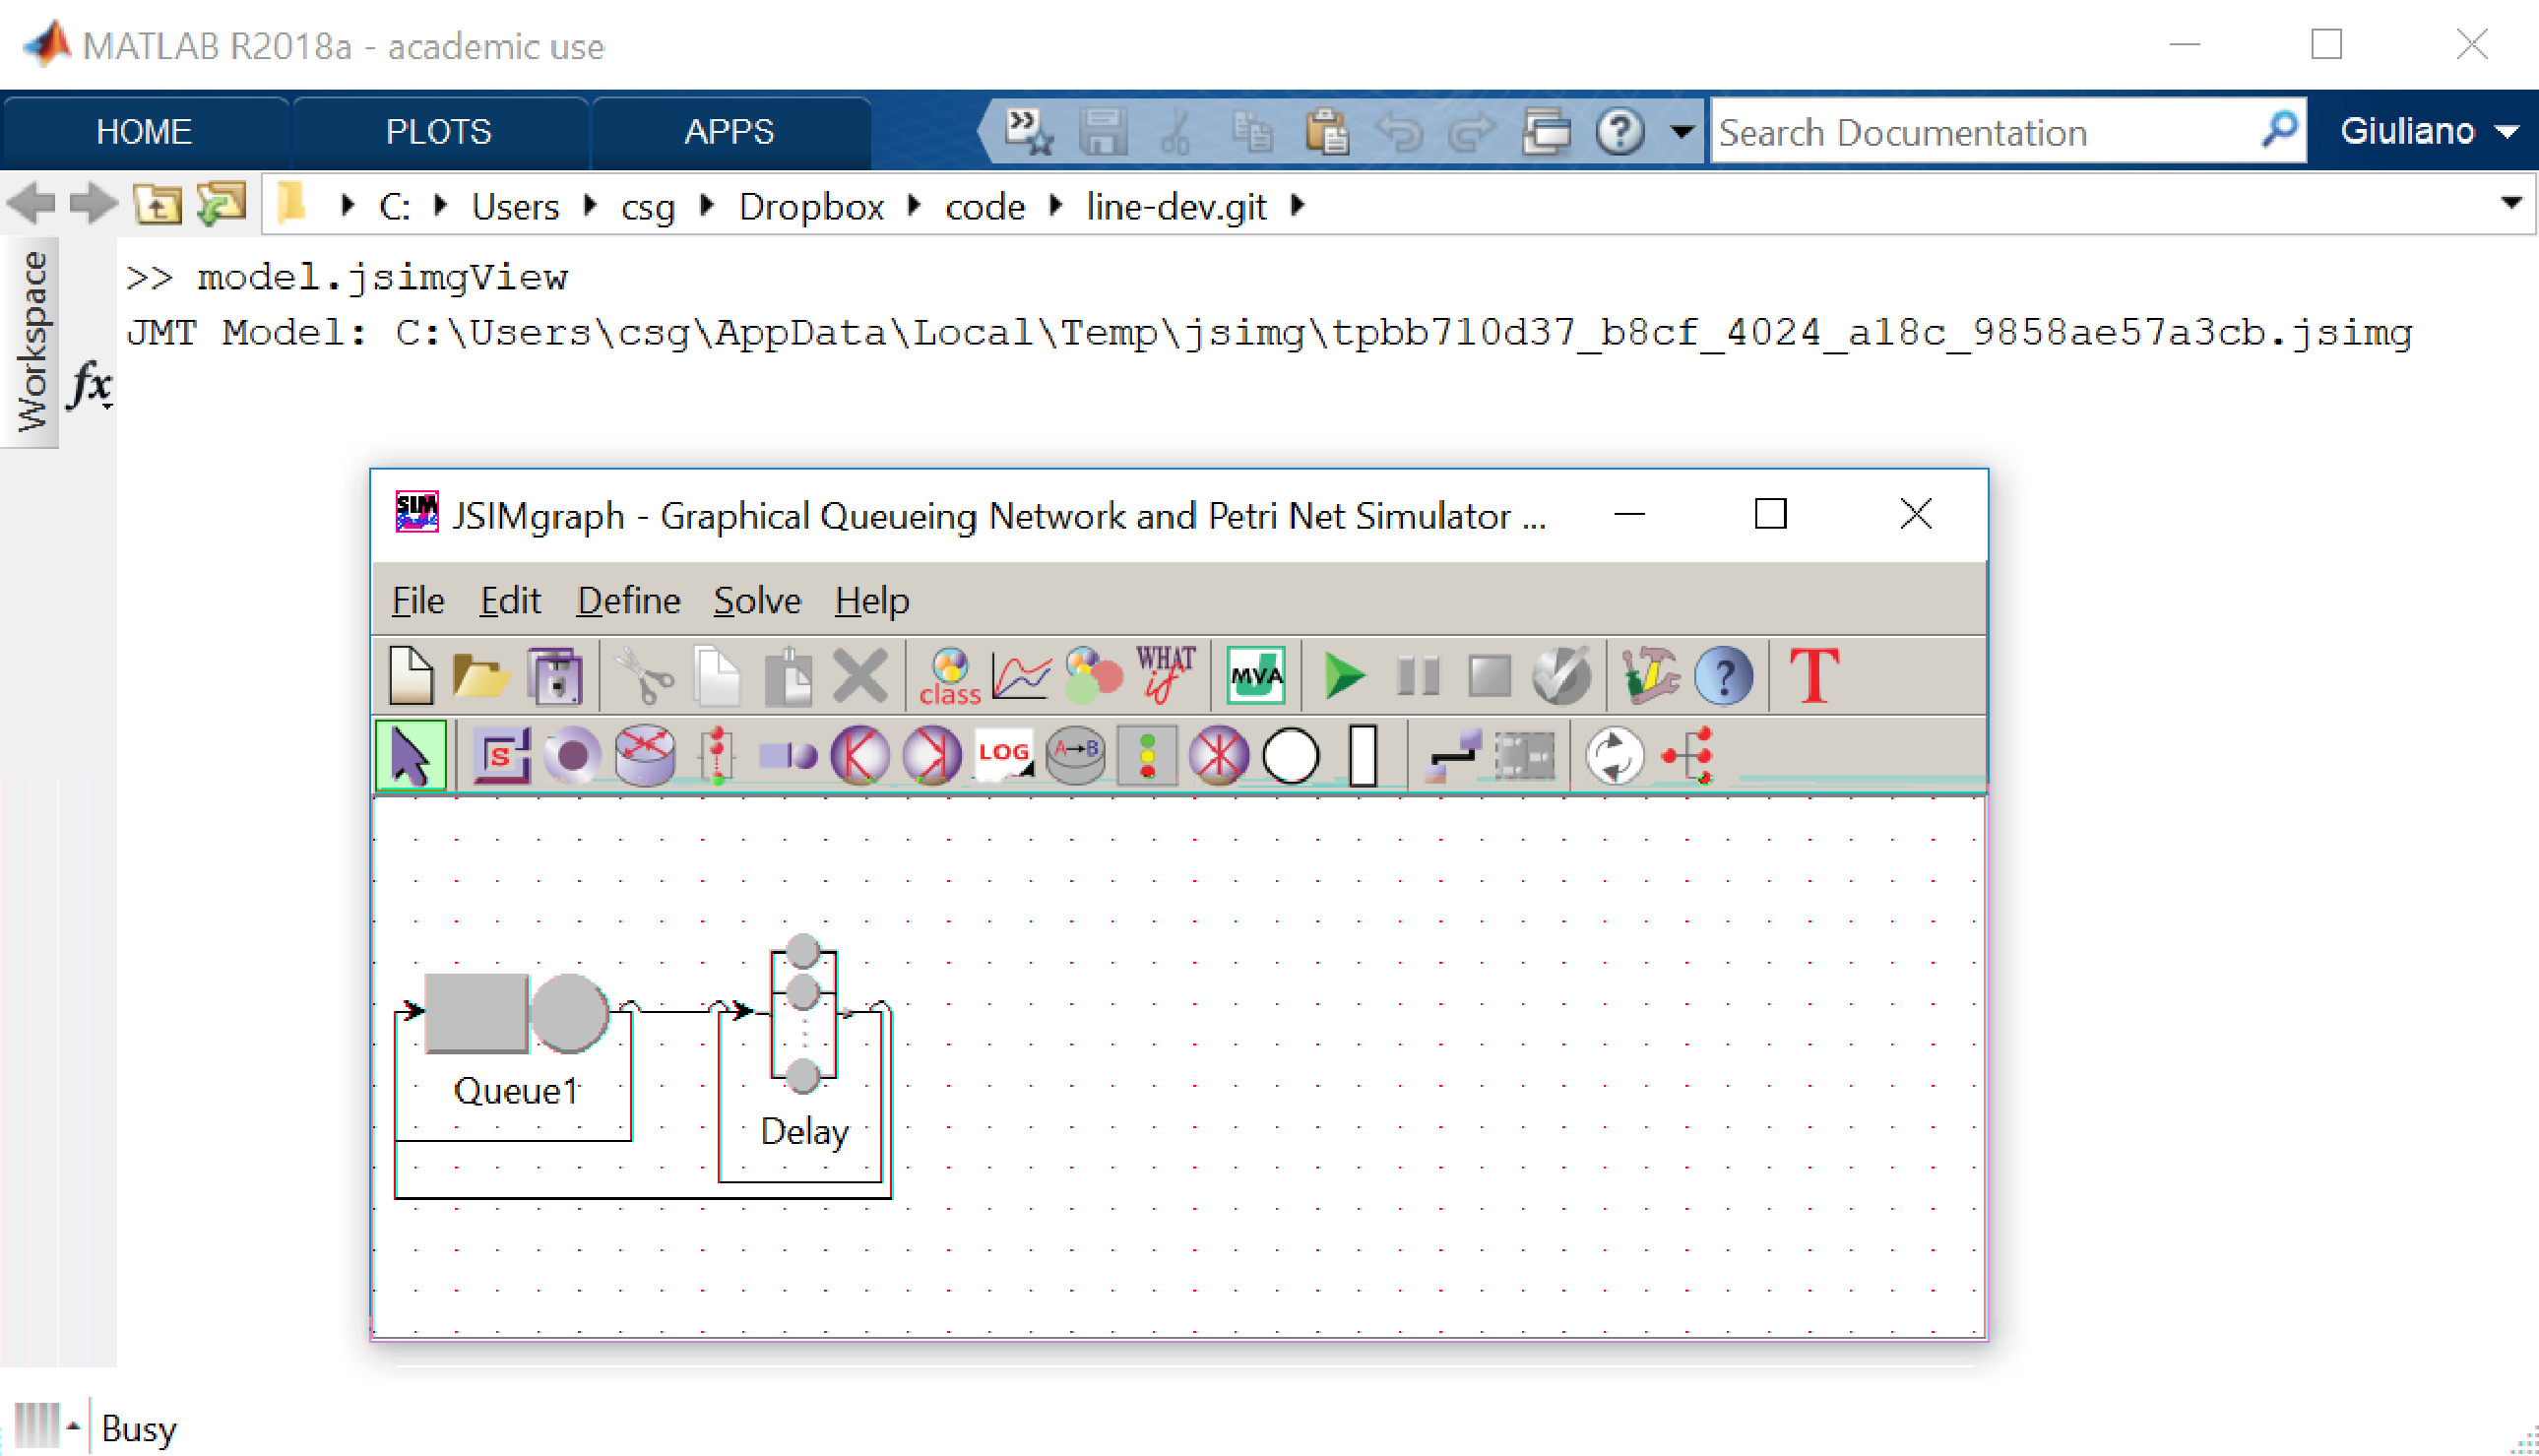
\includegraphics[width=14cm]{./images/jsimgView.pdf}
%  \caption{\texttt{Network.jsimgView} function}\label{FIG_jsimgView}
  \caption{\texttt{jsimgView} function}\label{jsimgView-function}
\end{figure}

\begin{MATLAB}
Another way to debug a \textsc{Line} model is to transform it into a graph object, e.g.
\begin{lstlisting}[language = matlab]
G = model.getGraph();
plot(G,'EdgeLabel',G.Edges.Weight,'Layout','Layered')
\end{lstlisting}
plots a graph of the network topology in term of stations only. In a similar manner, the following variant of the same command shows the model in terms of nodes, which corresponds to the internal representation within \textsc{Line}.
\begin{lstlisting}[language = matlab]
[~,H] = model.getGraph();
plot(H,'EdgeLabel',H.Edges.Weight,'Layout','Layered')
\end{lstlisting}
The latter example is invoked by default if we type

\begin{lstlisting}[language = matlab]
plot(model)
\end{lstlisting}
which also adds automatic node coloring to highlight the class-switch nodes.

Figure~\ref{FIG_getGraph} shows the difference between the two commands for an open queueing network with two classes and class-switching. Weights on the edges correspond to routing probabilities. In the station topology on the left, note that since the \Matlab{Sink} node is not a station, departures to the \Matlab{Sink} are drawn as returns to the \Matlab{Source}. The node topology on the right, illustrates all nodes, including  \texttt{ClassSwitch} nodes that are automatically added by \textsc{Line} to apply the class-switching routing strategy. Double arcs between nodes indicate that both classes are routed to the destination.
\begin{figure}
  \centering
  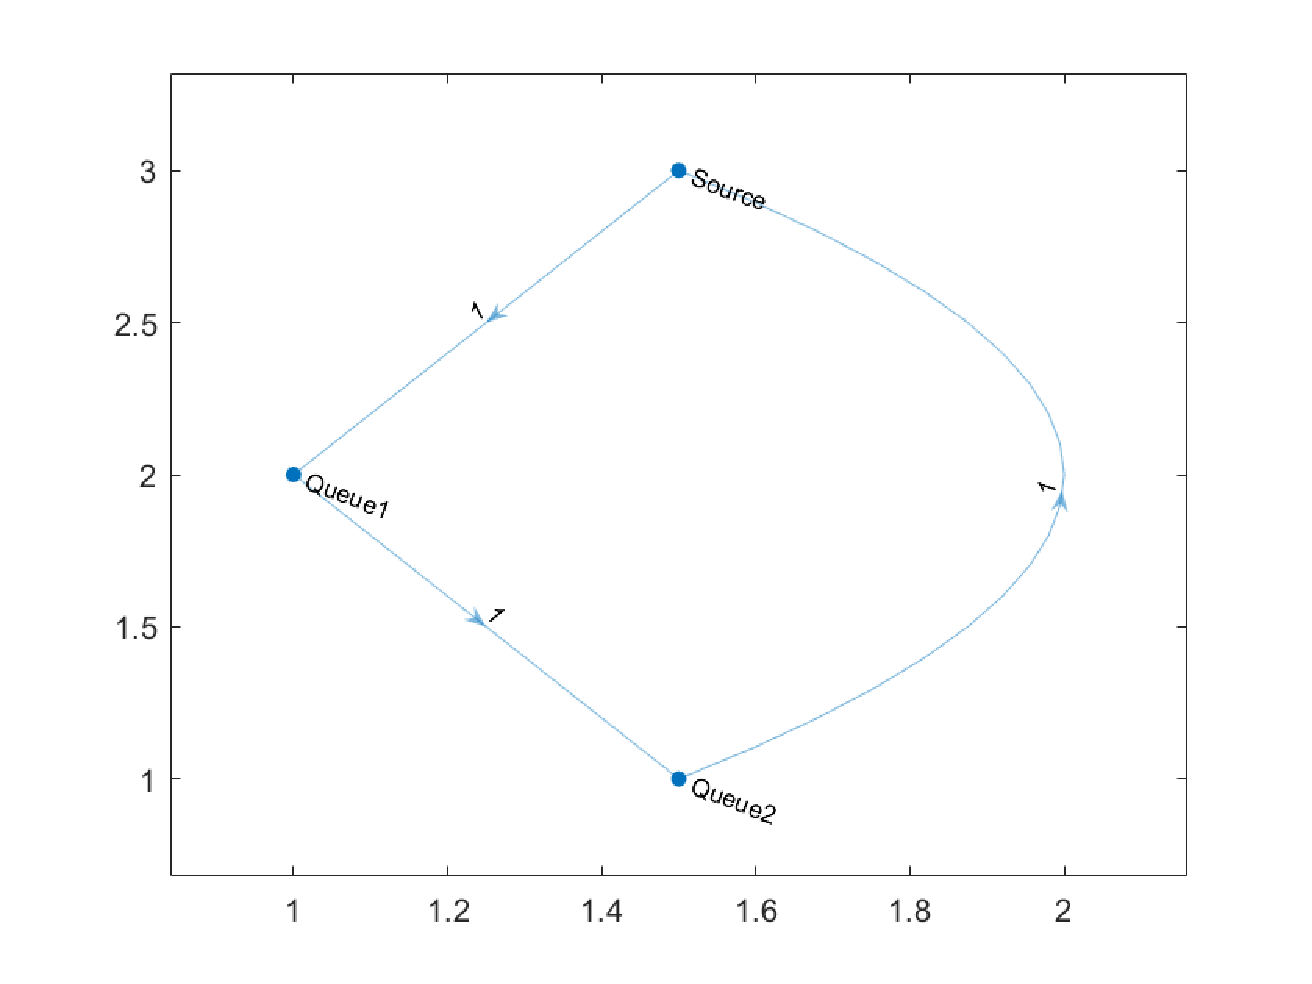
\includegraphics[width=7cm]{./images/getGraph_Stations.pdf}
  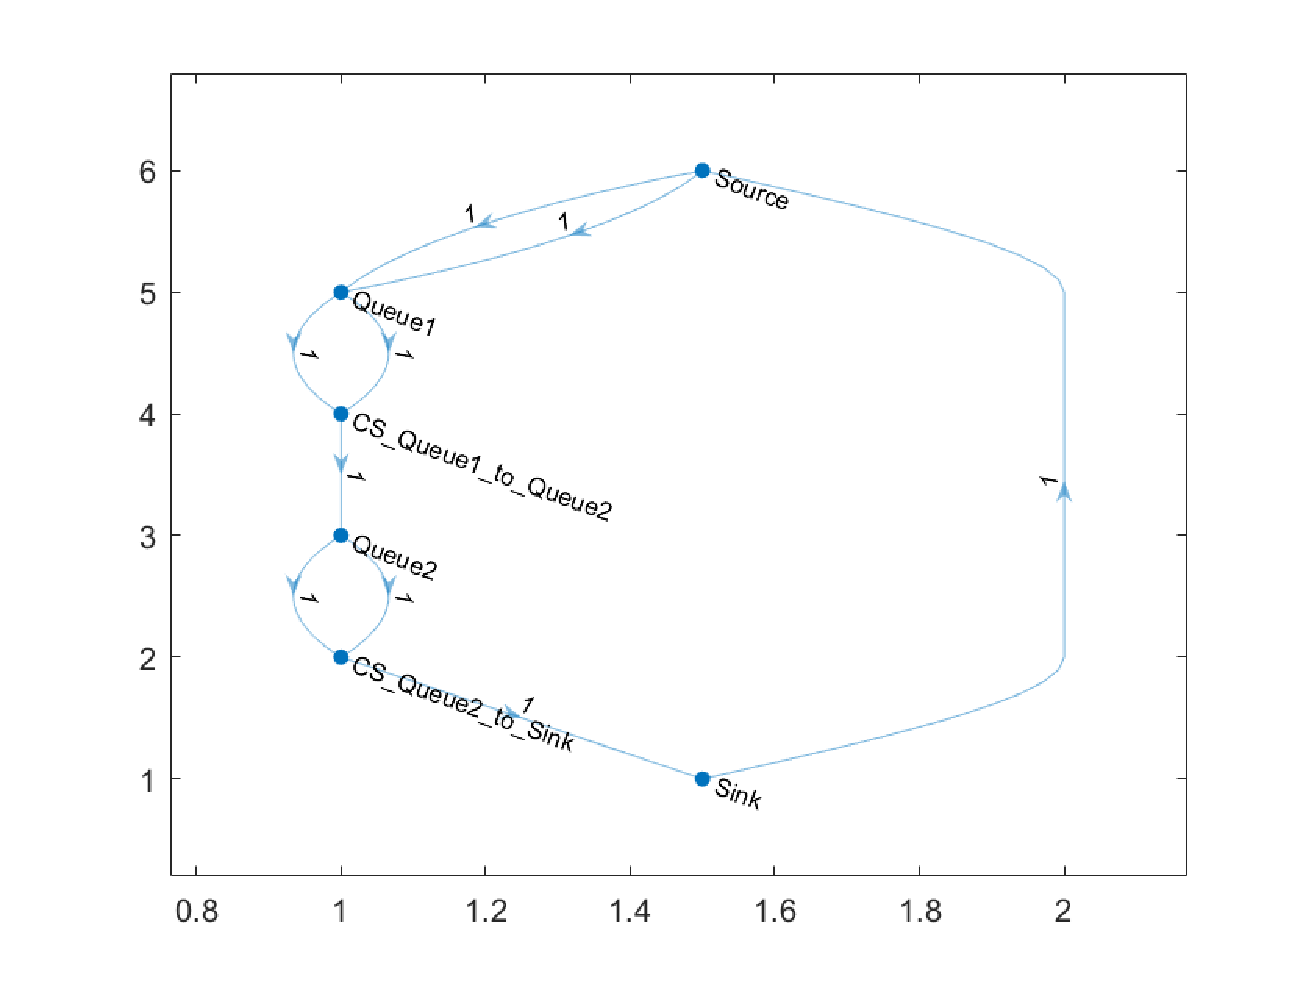
\includegraphics[width=7cm]{./images/getGraph_Nodes.pdf}
  \caption{\texttt{getGraph} function: station topology (left) and node topology (right) for a 2-class tandem queueing network with class-switching.}\label{FIG_getGraph}
\end{figure}

Furthermore, the graph properties concisely summarize the key features of the network
\begin{lstlisting}[language = matlab]
>> G.Nodes
ans =
  2x5 table
      Name            Type           Sched    Jobs    ClosedClass1
    ________    _________________    _____    ____    ____________
    'Delay'     'Delay'     		 'inf'     5           1
    'Queue1'    'Queue'  			 'ps'      0           2
>> G.Edges
ans =
  3x4 table
          EndNodes          Weight    Rate        Class
    ____________________    ______    ____    ______________
    'Delay'     'Delay'      0.7        1     'ClosedClass1'
    'Delay'     'Queue1'     0.3        1     'ClosedClass1'
    'Queue1'    'Delay'        1      0.5     'ClosedClass1'
\end{lstlisting}
Here, \texttt{Edge.Weight} is the routing probability between the nodes, whereas \texttt{Edge.Rate} is the service rate of the node appearing in the first column under \texttt{EndNodes}.
\end{MATLAB}
Another way to debug a \textsc{Line} model is to transform it into a graph object, i.e.,
\begin{JAVA}
\begin{lstlisting}[language=java, basicstyle=\ttfamily\scriptsize]
// Display graph edges
Graph G = model.getGraph();
System.out.println("Nodes: " + G.getNodes());
System.out.println("Edges: " + G.getEdges());
\end{lstlisting}
\end{JAVA}
\begin{KOTLIN}
Another way to debug a \textsc{Line} model is to transform it into a graph object, i.e.,
\begin{lstlisting}[language=kotlin, basicstyle=\ttfamily\scriptsize]
// Display graph edges
Graph G = model.getGraph();
System.out.println("Nodes: " + G.getNodes());
System.out.println("Edges: " + G.getEdges());
\end{lstlisting}
\end{KOTLIN}
\begin{PYTHON}
Another way to debug a \textsc{Line} model is to transform it into a graph object, i.e.,
\begin{lstlisting}[language = python]
# Display graph edges
G = model.get_graph()
print(f'Nodes: {G.nodes()}')
print(f'Edges: {G.edges(data=True)}')
\end{lstlisting}
\end{PYTHON}

\section{Model import and export}
%\section{Importing from BPMN}
%\section{Importing from JMT}
\textsc{Line} offers a number of scripts to import external models into \texttt{Network} object instances that can be analyzed through its solvers. %Similarly, a script is offered to convert a \Matlab{Network} object instance into a MATLAB \texttt{.m} file for later re-use.
The available scripts are as follows:
\begin{itemize}
\item \texttt{JMT2LINE} imports a JMT simulation model (\texttt{.jsimg} or \texttt{.jsimw} file) instance.
%\item \texttt{PMIF2LINE} imports an XML file containing a PMIF 1.0 model.
\end{itemize}
This script requires in input the filename and desired model name, and returns a single output, e.g.,
\begin{MATLAB}
%sn = PMIF2LINE([pwd,'\\examples\\data\\PMIF\\pmif_example_closed.xml'],'Mod1')
\begin{lstlisting}[language = matlab]
sn = JMT2LINE([pwd,'\\examples\\data\\JMT\\jmt_example.jsimg'],'Mod1')
\end{lstlisting}
\end{MATLAB}
\begin{JAVA}
\begin{lstlisting}[language=java, basicstyle=\ttfamily\scriptsize]
Network sn = JMT2LINE.load("examples/data/JMT/jmt_example.jsimg", "Mod1");
\end{lstlisting}
\end{JAVA}
\begin{KOTLIN}
\begin{lstlisting}[language=kotlin, basicstyle=\ttfamily\scriptsize]
Network sn = JMT2LINE.load("examples/data/JMT/jmt_example.jsimg", "Mod1");
\end{lstlisting}
\end{KOTLIN}
\begin{PYTHON}
\begin{lstlisting}[language=python]
sn = JMT2LINE.load('examples/data/JMT/jmt_example.jsimg', 'Mod1')
\end{lstlisting}
\end{PYTHON}
where \texttt{sn} is an instance of the \Matlab{Network} class.

\paragraph{JSON model serialization.}
\textsc{Line} models can be saved to and loaded from a portable JSON format conforming to the \texttt{line-model.schema.json} specification.  This enables model exchange across codebases and integration with external tools.  Supported model types include \texttt{Network}, \texttt{LayeredNetwork}, \texttt{Workflow}, and \texttt{Environment}.
\begin{MATLAB}
\begin{lstlisting}[language = matlab]
linemodel_save(model, 'mymodel.json');     % save
model = linemodel_load('mymodel.json');     % load
\end{lstlisting}
\end{MATLAB}
\begin{JAVA}
\begin{lstlisting}[language=java, basicstyle=\ttfamily\scriptsize]
LineModelSave.save(model, "mymodel.json");  // save
Network model = LineModelLoad.load("mymodel.json"); // load
\end{lstlisting}
\end{JAVA}
\begin{KOTLIN}
\begin{lstlisting}[language=kotlin, basicstyle=\ttfamily\scriptsize]
LineModelSave.save(model, "mymodel.json")   // save
val model = LineModelLoad.load("mymodel.json") // load
\end{lstlisting}
\end{KOTLIN}
\begin{PYTHON}
\begin{lstlisting}[language=python]
from line_solver.io import save_model, load_model
save_model(model, 'mymodel.json')           # save
model = load_model('mymodel.json')          # load
\end{lstlisting}
\end{PYTHON}

Beyond JMT models, \textsc{Line} supports importing workflow models specified using the Business Process Model and Notation (BPMN) 2.0 standard. BPMN is a widely adopted graphical notation for describing business processes and workflows, and its conversion to layered queueing networks enables performance analysis of process execution scenarios. The BPMN import capability transforms workflow elements into corresponding LayeredNetwork components that capture the essential performance characteristics of the process. In the conversion process, BPMN tasks are mapped to entries and activities in layered queueing networks, while BPMN resources become processors with associated scheduling policies. Parallel gateways in BPMN workflows are represented using AND-fork and AND-join precedence constructs within activity graphs, allowing the analysis of concurrent execution paths and their synchronization points. The multiplicity and replication settings of tasks and processors are derived from the resource allocation specified in the BPMN model. Service time distributions for activities are extracted from annotations or default exponential distributions are assigned when timing information is not explicitly provided. The reference to the MATLAB example file \texttt{lqn\_bpmn.m} in the examples directory demonstrates a complete workflow that has been manually converted from BPMN specification to a LayeredNetwork representation, illustrating the correspondence between workflow constructs and layered queueing network elements. This example shows how processors, tasks, entries, and activities are structured to preserve the precedence relationships and resource consumption patterns of the original business process. While automated import from BPMN XML files is supported through parsing utilities, manual model construction following the patterns in \texttt{lqn\_bpmn.m} provides greater control over the mapping of workflow semantics to performance model constructs. The ability to import and analyze BPMN models extends the applicability of \textsc{Line} to enterprise application performance modeling, business process optimization, and service-oriented architecture analysis.

\begin{MATLAB}
\Matlab{Network} object can be saved in binary \texttt{.mat} files using MATLAB's standard \texttt{save} command. However, it is also possible to export a textual script that will dynamically recreate the same \Matlab{Network} object. For example,
\begin{lstlisting}[language = matlab]
cqn_repairmen; LINE2MATLAB(model, 'script.m')
\end{lstlisting}
\end{MATLAB}
\begin{JAVA}
\end{JAVA}
\begin{KOTLIN}
\end{KOTLIN}
\begin{PYTHON}
\end{PYTHON}
\begin{MATLAB}
creates a new file \texttt{script.m} with code
\begin{lstlisting}[language = matlab]
model = Network('model');

%% Block 1: nodes
node{1} = DelayStation(model, 'Delay');
node{2} = Queue(model, 'Queue1', SchedStrategy.FCFS);

%% Block 2: classes
jobclass{1} = ClosedClass(model, 'Class1', 10, node{1}, 0);

node{1}.setService(jobclass{1}, Exp.fitMean(1.000000)); % (Delay,Class1)
node{2}.setService(jobclass{1}, Exp.fitMean(1.500000)); % (Queue1,Class1)

%% Block 3: topology
P = model.initRoutingMatrix(); % initialize routing matrix
P{1,1}(1,1) = 7.000000e-01; % (Delay,Class1) -> (Delay,Class1)
P{1,1}(1,2) = 3.000000e-01; % (Delay,Class1) -> (Queue1,Class1)
P{1,1}(2,1) = 1; % (Queue1,Class1) -> (Delay,Class1)
model.link(P);
\end{lstlisting}
that is equivalent to the model specified in \texttt{cqn\_repairmen.m}.
\end{MATLAB}
\begin{JAVA}
\end{JAVA}
\begin{KOTLIN}
\end{KOTLIN}
\begin{PYTHON}
\end{PYTHON}

\begin{MATLAB}
\subsection{Creating a \textsc{Line} model using JMT}
Using the features presented in the previous section, one can create a model in JMT and automatically derive a corresponding \textsc{Line} script from it. For instance, the following command performs the import and translation into a script, e.g.,
\begin{lstlisting}[language = matlab]
LINE2MATLAB(JMT2LINE('myModel.jsimg'),'myModel.m')
\end{lstlisting}
transforms and save the given JSIMgraph model into a corresponding \textsc{Line} model.

\textsc{Line} also provides two static functions to inspect \texttt{jsimg} and \texttt{jsimw} files before conversion, called
\texttt{JMT.jsimgOpen} and \texttt{JMT.jsimwOpen} require as an input parameter only the JMT file name, e.g., myModel.jsimg.

It is also possible to automate the editing and import of JMT models from MATLAB using the \texttt{jsimgEdit} command. This will open an empty JMT model and upon saving this will be automatically reimported into MATLAB.
\end{MATLAB}
\begin{JAVA}
\end{JAVA}
\begin{KOTLIN}
\end{KOTLIN}
\begin{PYTHON}
\end{PYTHON}

\subsection{Supported JMT features}
Table~\ref{TAB_JMT2LINE} lists the JSIMgraph/JSIMwiz model features supported by the \texttt{JMT2LINE} transformation. We indicate as ``Fully'' supported a feature that is supported in the import and such that the resulting model can be solved in \textsc{Line} using at least \texttt{JMT}. A feature with ``Partial'' support implies that some core aspects of this feature available in JSIM are not available in \textsc{Line}.

A few notes are needed to clarify the entries with partial support:
\begin{itemize}
\item \texttt{Fork} and \texttt{Join} are supported with their default policies. Advanced policies, such as partial joins or setting a distribution for the forked tasks on each output link, are not supported yet.
\item a single \texttt{Sink} and a single \texttt{Source} can be instantiated in a \textsc{Line} model, whereas there is no such constraint in JMT.
\end{itemize}

{\scriptsize
\renewcommand{\arraystretch}{1.2}
\begin{longtable}{|p{0.20\linewidth}|p{0.15\linewidth}|p{0.60\linewidth}|}
\caption{Supported JSIM features for automated model import and analysis}\\
\hline
\textbf{JMT Feature} & \textbf{Support} & \textbf{Notes} \\
\hline
\endfirsthead
\multicolumn{3}{c}{\tablename\ \thetable\ -- \textit{Continued from previous page}} \\
\hline
\textbf{JMT Feature} & \textbf{Support} & \textbf{Notes} \\
\hline
\endhead
\hline \multicolumn{3}{r}{\textit{Continued on next page}} \\
\endfoot
\hline
\endlastfoot
Distributions & Full & Phase-Type, Burst (MAP), Burst (MMPP2), Matrix Exponential (ME), Rational Arrival Process (RAP), Deterministic, Disabled, Exponential, Erlang, Gamma, Hyperexponential, Coxian, Logistic, Pareto, Uniform, Zero Service Time, Replayer, Weibull\\
Classes  & Full & Open class, Closed class, Class priorities\\
Metrics & Full & Number of customers, Residence Time, Throughput, Response Time, Throughput per sink, Utilization, Arrival Rate\\
Nodes & Full & Finite Capacity Region, ClassSwitch, Place, Delay, Logger, Queue, Router, Transition\\
Routing & Full & Random, Probabilities, Round Robin, Join the Shortest Queue \\
Mechanisms & Full & Polling, Setup times, Delay-off times, Switchover times, Impatience, Load Dependence, Retrial, Soft deadlines, Heterogeneous servers, Server Compatibilities \\
Scheduling & Full & FCFS, FCFSPRIO, LCFS, LCFS-PR, SIRO (Random), SJF, SEPT, LJF, LEPT, PS, DPS, GPS, PS Priority, DPS Priority, GPS Priority, LPS, EDD, EDF, SRPT \\
\hline
%Distributions & Partial & Phase-Type\\
%Classes  & Partial & \\
Nodes & Partial & Fork, Join, Source, Sink\\
%Routing & Partial & \\
%Scheduling & Partial & \\
\hline
Distributions & No & Burst (General), Normal\\
%Classes  & No & \\
Nodes & No & Scaler, Semaphore\\
Routing & No & Shortest Response Time, Least Utilization, Fastest Service, Load Dependent, Class Switch Routing \\
Metrics & No & Drop rate, Response time per sink, Power\\
Scheduling & No & TBS, QBPS\\
Mechanisms & No & Parallelism \\
%ClassSwitch & $\checkmark$ & \\
%Delay & $\checkmark$ & \\
%FCR & & Finite Capacity Region\\
%Fork & & \\
%Join & & \\
%Logger & & \\
%Place & & \\
%Queue & $\checkmark$ & \\
%Router & $\checkmark$ & \\
%Scaler & & \\
%Semaphore & & \\
%Sink & $\checkmark$ & \\
%Source & $\checkmark$ & \\
%Transition & & \\
\hline
\end{longtable}
\label{TAB_JMT2LINE}
}

\section{Finite capacity regions}
A Finite Capacity Region (FCR) provides a mechanism to constrain the total number of jobs that can simultaneously reside within a designated group of stations in a queueing network. Unlike per-station buffer limits, which restrict occupancy at individual queues, an FCR imposes a collective constraint across multiple stations, limiting the aggregate number of jobs across all stations in the region. When the region reaches its capacity, incoming jobs are either dropped or blocked depending on the configured drop strategy. This modeling capability is particularly useful for representing systems with admission control policies, finite buffers spanning multiple processing stages, resource constraints that affect groups of servers, or loss networks where jobs are rejected when the system lacks sufficient capacity.

An FCR is created using the \Matlab{\texttt{addRegion}}\Java{\texttt{addRegion}}\Kotlin{\texttt{addRegion}}\Python{\texttt{add\_region}} method of the \texttt{Network} class, which takes as input a cell array or list of stations belonging to the region. The maximum occupancy across all stations in the region is set via \Matlab{\texttt{setGlobalMaxJobs}}\Java{\texttt{setGlobalMaxJobs}}\Kotlin{\texttt{setGlobalMaxJobs}}\Python{\texttt{set\_global\_max\_jobs}}, which specifies the total number of jobs allowed in the region. The drop behavior for each class is configured using \Matlab{\texttt{setDropRule}}\Java{\texttt{setDropRule}}\Kotlin{\texttt{setDropRule}}\Python{\texttt{set\_drop\_rule}}, which determines whether arriving jobs are dropped when the region is at capacity.

\begin{MATLAB}
\begin{lstlisting}[language = matlab]
fcr = model.addRegion({queue1, queue2});
fcr.setGlobalMaxJobs(K);
fcr.setDropRule(jobclass1, true);  % true = drop jobs when region full
\end{lstlisting}
\end{MATLAB}
\begin{JAVA}
\begin{lstlisting}[language=java, basicstyle=\ttfamily\scriptsize]
Region fcr = model.addRegion(Arrays.asList(queue1, queue2));
fcr.setGlobalMaxJobs(K);
fcr.setDropRule(jobclass1, true);  // true = drop jobs when region full
\end{lstlisting}
\end{JAVA}
\begin{KOTLIN}
\begin{lstlisting}[language=kotlin, basicstyle=\ttfamily\scriptsize]
val fcr = model.addRegion(listOf(queue1, queue2))
fcr.setGlobalMaxJobs(K)
fcr.setDropRule(jobclass1, true)  // true = drop jobs when region full
\end{lstlisting}
\end{KOTLIN}
\begin{PYTHON}
\begin{lstlisting}[language=python]
fcr = model.add_region([queue1, queue2])
fcr.set_global_max_jobs(K)
fcr.set_drop_rule(jobclass1, True)  # True = drop jobs when region full
\end{lstlisting}
\end{PYTHON}

Two primary drop strategies are available. The \texttt{DropStrategy.Drop} strategy causes jobs to be permanently lost when they arrive at a full region, modeling systems where arrivals are rejected or abandoned. The \texttt{DropStrategy.WaitingQueue} strategy causes jobs to wait in a virtual queue until capacity becomes available, modeling systems with admission control or backpressure mechanisms. In addition to global capacity constraints, per-class capacity limits can be specified within a region to enforce class-specific occupancy restrictions.

A special case of interest is an FCR containing a single queue with dropping enabled. This configuration behaves identically to an M/M/1/K queue, where K is the maximum capacity including both jobs in service and jobs waiting in the buffer. This equivalence provides a convenient way to model loss systems and finite-buffer queues. The examples \texttt{fcr\_mm1kdrop}, \texttt{fcr\_mm1waitq}, \texttt{fcr\_constraints}, and \texttt{fcr\_oqndrop} demonstrate various applications of finite capacity regions, including single-queue finite buffers, multi-station regions with different drop policies, and open queueing networks with job loss.

When using the \texttt{JMT} solver, two additional performance metrics can be requested for each FCR. The \texttt{FCRWeight} metric (\texttt{MetricType.FCRWeight}) reports the total weight of jobs currently residing in the region, which is useful when jobs are assigned heterogeneous weights reflecting their resource consumption (e.g., memory footprint or storage size). The \texttt{FCRMemOcc} metric (\texttt{MetricType.FCRMemOcc}) reports the total memory occupation of the region, aggregating the memory contributions of all jobs present across the stations in the region. These metrics are particularly relevant when modeling cache-like systems or storage pools where different job classes consume different amounts of shared resources.

\section{Reward models}
\textsc{Line} supports the definition of custom reward functions on network models, enabling the computation of application-specific performance metrics beyond the standard measures of queue length, utilization, and response time. Rewards associate a numerical value with each state of the underlying continuous-time Markov chain, allowing analysts to define metrics that capture domain-specific objectives such as energy consumption, revenue, or composite performance indicators. The reward framework supports both steady-state analysis, which computes the expected reward in equilibrium, and transient analysis, which tracks the evolution of reward values over time. This feature is available through the \texttt{CTMC} solver, which constructs the Markov chain representation of the network and evaluates reward functions over the state space.

Reward functions are defined using the \Matlab{\texttt{setReward}}\Java{\texttt{setReward}}\Kotlin{\texttt{setReward}}\Python{\texttt{set\_reward}} method on the \texttt{Network} object. This method takes two arguments: a string name for the reward, which is used to identify it in the results, and a function that maps a state accessor object to a scalar reward value. The state accessor provides the method \Matlab{\texttt{at}}\Java{\texttt{at}}\Kotlin{\texttt{at}}\Python{\texttt{at}}, which takes a node and a job class as arguments and returns the number of jobs of that class at that node in the current state.

\begin{MATLAB}
\begin{lstlisting}[language = matlab]
model.setReward('QueueLength', @(state) state.at(queue, oclass));
\end{lstlisting}
\end{MATLAB}
\begin{JAVA}
\begin{lstlisting}[language=java, basicstyle=\ttfamily\scriptsize]
model.setReward("QueueLength", state -> state.at(queue, oclass));
\end{lstlisting}
\end{JAVA}
\begin{KOTLIN}
\begin{lstlisting}[language=kotlin, basicstyle=\ttfamily\scriptsize]
model.setReward("QueueLength") { state -> state.at(queue, oclass) }
\end{lstlisting}
\end{KOTLIN}
\begin{PYTHON}
\begin{lstlisting}[language=python]
model.set_reward('QueueLength', lambda state: state.at(queue, oclass))
\end{lstlisting}
\end{PYTHON}

This example defines a reward equal to the number of jobs of class \texttt{oclass} at the \texttt{queue} node. More complex reward functions can be constructed by combining state information from multiple nodes and classes, or by applying arbitrary mathematical operations to state variables.

To simplify common use cases, \Matlab{\textsc{Line} provides pre-built reward templates through the \texttt{Reward} class. The \texttt{Reward.utilization} method creates}\Java{equivalent reward functions can be expressed using lambda expressions implementing the \texttt{RewardFunction} interface. A utilization reward creates}\Kotlin{equivalent reward functions can be expressed using lambda expressions implementing the \texttt{RewardFunction} interface. A utilization reward creates}\Python{\textsc{Line} provides pre-built reward templates through the \texttt{Reward} class. The \texttt{Reward.utilization} method creates} a reward function that returns an indicator variable, taking the value 1 when the specified node is serving a job of the specified class and 0 otherwise. The \Matlab{\texttt{Reward.blocking}}\Java{blocking reward}\Kotlin{blocking reward}\Python{\texttt{Reward.blocking}} method creates a reward function that returns an indicator for buffer-full conditions, taking the value 1 when the node's buffer is at capacity and 0 otherwise.

\begin{MATLAB}
\begin{lstlisting}[language = matlab]
model.setReward('Utilization', Reward.utilization(queue, oclass));
model.setReward('BlockingProb', Reward.blocking(queue));
\end{lstlisting}
\end{MATLAB}
\begin{JAVA}
\begin{lstlisting}[language=java, basicstyle=\ttfamily\scriptsize]
model.setReward("Utilization", (state, sn) -> {
    int ist = sn.nodeToStation[(int) queue.getNodeIdx()];
    double n = state.get(0, (int) oclass.getIndex());
    return Math.min(n, sn.nservers.get(ist));
});
\end{lstlisting}
\end{JAVA}
\begin{KOTLIN}
\begin{lstlisting}[language=kotlin, basicstyle=\ttfamily\scriptsize]
model.setReward("Utilization") { state, sn ->
    val ist = sn.nodeToStation[queue.nodeIdx.toInt()]
    val n = state[0, oclass.index.toInt()]
    minOf(n, sn.nservers[ist].toDouble())
}
\end{lstlisting}
\end{KOTLIN}
\begin{PYTHON}
\begin{lstlisting}[language=python]
model.set_reward('Utilization', Reward.utilization(queue, oclass))
model.set_reward('BlockingProb', Reward.blocking(queue))
\end{lstlisting}
\end{PYTHON}

Once reward functions are defined on the model, they can be evaluated by creating a \texttt{CTMC} solver instance and calling the appropriate analysis methods. For steady-state analysis, the \Matlab{\texttt{getAvgReward}}\Java{\texttt{getAvgReward}}\Kotlin{\texttt{getAvgReward}}\Python{\texttt{get\_avg\_reward}} method returns \Matlab{a vector of expected reward values in equilibrium, along with a cell array of reward names}\Java{a map from reward names to their expected values in equilibrium}\Kotlin{a map from reward names to their expected values in equilibrium}\Python{a vector of expected reward values in equilibrium, along with a list of reward names}. For transient analysis, the \Matlab{\texttt{getReward}}\Java{\texttt{getRewardResult}}\Kotlin{\texttt{getRewardResult}}\Python{\texttt{get\_reward}} method returns \Matlab{time-indexed reward trajectories, along with the time points, reward names, and the state space representation}\Java{a \texttt{RewardResult} object containing value functions, time vector, reward names, state space, and steady-state values}\Kotlin{a \texttt{RewardResult} object containing value functions, time vector, reward names, state space, and steady-state values}\Python{time-indexed reward trajectories, along with the time points, reward names, and the state space representation}.

\begin{MATLAB}
\begin{lstlisting}[language = matlab]
solver = CTMC(model, options);
[R, names] = solver.getAvgReward();   % steady-state expected rewards
[t, V, names, stateSpace] = solver.getReward();  % transient trajectories
\end{lstlisting}
\end{MATLAB}
\begin{JAVA}
\begin{lstlisting}[language=java, basicstyle=\ttfamily\scriptsize]
SolverCTMC solver = new SolverCTMC(model, options);
Map<String, Double> avgReward = solver.getAvgReward();  // steady-state
RewardResult rewardResult = solver.getRewardResult();  // transient
\end{lstlisting}
\end{JAVA}
\begin{KOTLIN}
\begin{lstlisting}[language=kotlin, basicstyle=\ttfamily\scriptsize]
val solver = SolverCTMC(model, options)
val avgReward = solver.getAvgReward()  // steady-state: Map<String, Double>
val rewardResult = solver.getRewardResult()  // transient: RewardResult
\end{lstlisting}
\end{KOTLIN}
\begin{PYTHON}
\begin{lstlisting}[language=python]
solver = SolverCTMC(model, options)
R, names = solver.get_avg_reward()   # steady-state expected rewards
t, V, names, state_space = solver.get_reward()  # transient trajectories
\end{lstlisting}
\end{PYTHON}

The reward framework is particularly useful for defining objective functions in optimization problems, tracking custom performance indicators that combine multiple system states, or analyzing transient behavior of derived metrics. The examples \texttt{rewardModel\_basic}, \texttt{rewardModel\_templates}, and \texttt{rewardModel\_aggregation} demonstrate various applications of reward models, including simple state-based rewards, the use of template functions, and the aggregation of reward values across multiple nodes or classes.

\section{Stochastic Petri nets}
\textsc{Line} supports the specification of stochastic Petri net (SPN) models through dedicated \texttt{Place} and \texttt{Transition} node types, providing an alternative modeling paradigm to queueing networks. In an SPN, the system state is represented by the distribution of tokens across places, and the system dynamics are governed by transition firings that consume tokens from input places and produce tokens in output places. This formalism is particularly well-suited for modeling systems with synchronization, resource sharing, and complex control flow that may be difficult to express naturally in the queueing network framework.

A \texttt{Place} is a stateful node that holds tokens, which correspond to jobs in the queueing network interpretation. Places can have capacity limits and initial token populations. A \texttt{Transition} is a node that defines one or more firing modes, each representing a distinct way the transition can fire. Each mode has its own timing distribution, which governs the delay between enabling and firing, its own enabling condition, which specifies the number of tokens required in each input place, and its own firing outcome, which specifies the number of tokens deposited in each output place when the transition fires. The ability to define multiple modes on a single transition allows modeling of complex state-dependent behaviors and routing decisions.

The following example demonstrates the creation of a simple SPN model. A place \texttt{P1} and a transition \texttt{T1} are created, and a firing mode is added to the transition. The mode is configured with an exponential firing delay, an enabling condition requiring one token in \texttt{P1}, and a firing outcome producing one token in a sink node.

\begin{MATLAB}
\begin{lstlisting}[language = matlab]
P1 = Place(model, 'P1');
T1 = Transition(model, 'T1');
mode = T1.addMode('Mode1');
T1.setNumberOfServers(mode, Inf);
T1.setDistribution(mode, Exp(4));
T1.setEnablingConditions(mode, jobclass1, P1, 1);  % requires 1 token in P1
T1.setFiringOutcome(mode, jobclass1, sink, 1);     % produces 1 token in sink
\end{lstlisting}
\end{MATLAB}
\begin{JAVA}
\begin{lstlisting}[language=java, basicstyle=\ttfamily\scriptsize]
Place P1 = new Place(model, "P1");
Transition T1 = new Transition(model, "T1");
int mode = T1.addMode("Mode1");
T1.setNumberOfServers(mode, Integer.MAX_VALUE);
T1.setDistribution(mode, new Exp(4));
T1.setEnablingConditions(mode, jobclass1, P1, 1);  // requires 1 token in P1
T1.setFiringOutcome(mode, jobclass1, sink, 1);     // produces 1 token in sink
\end{lstlisting}
\end{JAVA}
\begin{KOTLIN}
\begin{lstlisting}[language=kotlin, basicstyle=\ttfamily\scriptsize]
val P1 = Place(model, "P1")
val T1 = Transition(model, "T1")
val mode = T1.addMode("Mode1")
T1.setNumberOfServers(mode, Int.MAX_VALUE)
T1.setDistribution(mode, Exp(4.0))
T1.setEnablingConditions(mode, jobclass1, P1, 1)  // requires 1 token in P1
T1.setFiringOutcome(mode, jobclass1, sink, 1)     // produces 1 token in sink
\end{lstlisting}
\end{KOTLIN}
\begin{PYTHON}
\begin{lstlisting}[language=python]
P1 = Place(model, 'P1')
T1 = Transition(model, 'T1')
mode = T1.add_mode('Mode1')
T1.set_number_of_servers(mode, float('inf'))
T1.set_distribution(mode, Exp(4))
T1.set_enabling_conditions(mode, jobclass1, P1, 1)  # requires 1 token in P1
T1.set_firing_outcome(mode, jobclass1, sink, 1)     # produces 1 token in sink
\end{lstlisting}
\end{PYTHON}

In addition to standard enabling conditions, SPN models support inhibiting arcs, which prevent a transition from firing when a place contains too many tokens. This mechanism is useful for modeling resource constraints or conditions where an event should not occur when a system is in a particular state. The \Matlab{\texttt{setInhibitingConditions}}\Java{\texttt{setInhibitingConditions}}\Kotlin{\texttt{setInhibitingConditions}}\Python{\texttt{set\_inhibiting\_conditions}} method specifies that a transition cannot fire when a designated place holds more than a specified threshold number of tokens.

\begin{MATLAB}
\begin{lstlisting}[language = matlab]
T1.setInhibitingConditions(mode, jobclass1, P2, 2);  % inhibit if P2 has >2 tokens
\end{lstlisting}
\end{MATLAB}
\begin{JAVA}
\begin{lstlisting}[language=java, basicstyle=\ttfamily\scriptsize]
T1.setInhibitingConditions(mode, jobclass1, P2, 2);  // inhibit if P2 has >2 tokens
\end{lstlisting}
\end{JAVA}
\begin{KOTLIN}
\begin{lstlisting}[language=kotlin, basicstyle=\ttfamily\scriptsize]
T1.setInhibitingConditions(mode, jobclass1, P2, 2)  // inhibit if P2 has >2 tokens
\end{lstlisting}
\end{KOTLIN}
\begin{PYTHON}
\begin{lstlisting}[language=python]
T1.set_inhibiting_conditions(mode, jobclass1, P2, 2)  # inhibit if P2 has >2 tokens
\end{lstlisting}
\end{PYTHON}

SPN models in \textsc{Line} are analyzed by the \texttt{JMT} solver, which translates the Petri net specification into its native simulation engine and performs discrete-event simulation to estimate performance metrics. This allows SPN models to benefit from \texttt{JMT}'s efficient simulation algorithms while retaining the expressive power of the Petri net formalism. The examples \texttt{spn\_basic\_open}, \texttt{spn\_twomodes}, \texttt{spn\_inhibiting}, and \texttt{spn\_closed\_fourplaces} demonstrate various applications of stochastic Petri nets, including open and closed systems, multi-mode transitions for state-dependent routing, inhibiting arcs for resource constraints, and complex token flows.

\section{Signals and G-networks}
\textsc{Line} supports the modeling of G-networks, also known as Gelenbe networks, through the \texttt{Signal} class. G-networks extend traditional queueing networks by introducing negative customers, which have the distinctive property of removing positive customers from queues upon arrival rather than joining them. This mechanism provides a natural way to model phenomena such as job cancellations, cache invalidations, service interrupts, or resets in computing systems. The interaction between positive and negative customers creates rich dynamics that capture feedback control, load regulation, and catastrophic events in networked systems.

A signal is defined using the \texttt{Signal} constructor, which takes a model reference, a descriptive name, and a signal type that specifies the behavior of the signal class. The \texttt{SignalType.NEGATIVE} type creates a negative customer class with the semantics that each arrival at a queue removes one positive customer from that queue. If the queue is empty when a negative customer arrives, the negative customer has no effect and is simply absorbed.

\begin{MATLAB}
\begin{lstlisting}[language = matlab]
negClass = Signal(model, 'Negative', SignalType.NEGATIVE);
source.setArrival(negClass, Exp(lambda_neg));
\end{lstlisting}
\end{MATLAB}
\begin{JAVA}
\begin{lstlisting}[language=java, basicstyle=\ttfamily\scriptsize]
Signal negClass = new Signal(model, "Negative", SignalType.NEGATIVE);
source.setArrival(negClass, new Exp(lambda_neg));
\end{lstlisting}
\end{JAVA}
\begin{KOTLIN}
\begin{lstlisting}[language=kotlin, basicstyle=\ttfamily\scriptsize]
val negClass = Signal(model, "Negative", SignalType.NEGATIVE)
source.setArrival(negClass, Exp(lambda_neg))
\end{lstlisting}
\end{KOTLIN}
\begin{PYTHON}
\begin{lstlisting}[language=python]
neg_class = Signal(model, 'Negative', SignalType.NEGATIVE)
source.set_arrival(neg_class, Exp(lambda_neg))
\end{lstlisting}
\end{PYTHON}

In this example, a negative customer class is created and assigned an arrival process at a source node. When negative customers arrive at queues in the network, they reduce the queue populations by removing positive customers. The routing of negative customers is specified using the same mechanisms as for ordinary job classes, allowing complex patterns of cancellation and control.

G-network models can be analyzed using the \texttt{MAM} solver with the INAP or INAPPLUS methods, which exploit the product-form structure of certain G-network configurations through the RCAT (Reversed Compound Agent Theorem) framework. Under specific conditions on the arrival and service processes, G-networks admit product-form solutions that allow efficient exact analysis without state-space explosion. This capability makes it possible to analyze large-scale G-networks with multiple positive and negative customer classes while maintaining tractability.

\begin{MATLAB}
\begin{lstlisting}[language = matlab]
options = SolverOptions();
options.method = 'inap';
solver = SolverMAM(model, options);
[QN, UN, RN, TN] = solver.getAvg();
\end{lstlisting}
\end{MATLAB}
\begin{JAVA}
\begin{lstlisting}[language=java, basicstyle=\ttfamily\scriptsize]
SolverOptions options = new SolverOptions();
options.method = "inap";
SolverMAM solver = new SolverMAM(model, options);
AvgTable avgTable = solver.getAvgTable();
\end{lstlisting}
\end{JAVA}
\begin{KOTLIN}
\begin{lstlisting}[language=kotlin, basicstyle=\ttfamily\scriptsize]
val options = SolverOptions()
options.method = "inap"
val solver = SolverMAM(model, options)
val avgTable = solver.getAvgTable()
\end{lstlisting}
\end{KOTLIN}
\begin{PYTHON}
\begin{lstlisting}[language=python]
options = SolverOptions(method='inap')
solver = SolverMAM(model, options)
QN, UN, RN, TN = solver.get_avg()
\end{lstlisting}
\end{PYTHON}

The example \texttt{ag\_gnetwork} demonstrates the construction and analysis of a G-network model with both positive customers and negative arrivals, illustrating how signal classes interact with ordinary job classes to produce non-trivial equilibrium behavior. G-networks are particularly useful for modeling systems with dynamic load control, self-regulation, or reset mechanisms, where the conventional queueing network paradigm does not naturally capture the feedback effects of cancellations and interruptions.

\chapter{Analysis methods}
\label{analysis-methods}

\section{Performance metrics}
As discussed earlier, \textsc{Line} supports a set of steady-state and transient performance metrics. Table~\ref{TAB_METRICS} summarizes the definition of the associated random variables. For each metric, one or more analysis types may be available, which are extensively discussed in the next sections.
\begin{table}[thbp]
\centering
{\scriptsize
\renewcommand{\arraystretch}{1.2}
\caption{Performance metrics} %{Legend: $i,j=$ stations; $r,s=$ classes; $c=$ chain; $k=$ phase; $t=$ state}}
\begin{tabular}{|l|l|p{0.5\linewidth}|}
\hline
\textbf{Metric} & \textbf{Acronym} & \textbf{Description} \\
\hline
Queue-length & \texttt{QLen}  & Number of jobs of class $r$ (or chain-$c$) residing at a node $i$\\
Utilization & \texttt{Util} & Utilization of class-$r$ (or chain-$c$) jobs at node $i$, scaled in [0,1] for multi-server nodes, equal to \texttt{QLen} at infinite server nodes\\
Response time & \texttt{RespT}  & Time that a class-$r$ (or chain-$c$) jobs spends for a single visit at node $i$\\
Residence time & \texttt{ResidT}  & Cumulative time that a class-$r$ (or chain-$c$) jobs spends across all visits at node $i$\\
Arrival rate & \texttt{ArvR} & Arrival rate of class-$r$ (or chain-$c$) jobs at node $i$\\
Throughput & \texttt{Tput} & Throughput of class-$r$ (or chain-$c$) jobs at node $i$\\
System Response time & \texttt{SysRespT}  & For an open chain $c$, this is the time from leaving the source to arriving at the sink for {\em any} class in the chain. For a closed chain $c$, this is the interval of time between two successive visits to the reference station in any two {\em completing classes} within the chain. \\
System Throughput & \texttt{SysTput} & For an open chain $c$, this is the departure rate towards the sink for {\em any} class in the chain. For a closed chain $c$, this is the rate of arrival of {\em completing classes} in the chain at the reference station. \\
System queue length & \texttt{SysQLen} & Total mean number of jobs in chain $c$ across all stations. For a closed chain, equal to the total number of jobs in the chain. For an open chain, related to \texttt{SysRespT} and \texttt{SysTput} through Little's law: $\mathtt{SysQLen}(c) = \mathtt{SysTput}(c) \cdot \mathtt{SysRespT}(c)$. \\
Fork-join queue length & \texttt{FJQLen} & Number of jobs present within a fork-join scope, counting from the moment they are dispatched at the fork until synchronization is completed at the join. Measured per fork-join pair. \\
Fork-join response time & \texttt{FJRespT} & Time from fork dispatch to completion of synchronization at the join, measuring the end-to-end latency of the parallel section across all spawned branches. \\
\hline
\end{tabular}
}
\label{TAB_METRICS}
\end{table}

\paragraph{Queue length in Finite Capacity Regions.}
When a station is part of a Finite Capacity Region (FCR) with \texttt{WaitingQueue} drop strategy, the reported queue length (\texttt{QLen}) includes both jobs currently inside the station and jobs that are blocked waiting to enter the FCR. This semantic ensures consistency with blocking queueing network models where blocked jobs are logically associated with their destination queue. For example, if an FCR with capacity 2 contains a queue with 2 jobs, and 1 additional job is blocked waiting to enter, the reported queue length will be 3. This convention is consistent with JMT's handling of FCR blocking.

\paragraph{Fork-join specific metrics.}
For models containing fork-join structures, \textsc{Line} provides specialized metrics that capture the end-to-end behavior of parallel execution sections. The \texttt{FJQLen} metric represents the queue length measured at the fork-join scope, counting jobs from the moment they are dispatched at the fork until their synchronization is completed at the join. This differs from standard per-station queue length metrics, which measure only the jobs residing at individual stations. Similarly, the \texttt{FJRespT} metric captures the response time from fork dispatch to join synchronization, measuring the total time required for all parallel tasks spawned by a fork to complete and synchronize. These metrics are essential for analyzing parallel processing systems, workflow applications, and distributed computing scenarios where understanding the aggregate behavior of forked execution paths is more relevant than individual station performance. Standard metrics measure individual station behavior in isolation, treating each queue or delay node independently. In contrast, fork-join metrics aggregate across all stations between a fork and its corresponding join, providing insight into the overall latency and resource consumption of parallel sections. These specialized metrics are reported through the standard \Matlab{\texttt{getAvgTable}}\Java{\texttt{getAvgTable}}\Kotlin{\texttt{getAvgTable}}\Python{\texttt{get\_avg\_table}} output when fork-join structures are present in the model. The fork-join metrics are computed by solvers that support fork-join modeling, including the MVA, JMT, and LDES solvers.

\section{Steady-state analysis}

\subsection{Station average performance}
\textsc{Line} decouples network specification from its solution, allowing to evaluate the same model with multiple solvers.
Model analysis is carried out in \textsc{Line} according to the following general steps:
\begin{description}
\item[Step 1: Definition of the model.] This proceeds as explained in the previous chapters.
\item[Step 2: Instantiation of the solver(s).] A solver is an instance of the \texttt{Solver} class. \textsc{Line} offers multiple solvers, which can be configured through a set of common and individual solver options. For example,
\begin{MATLAB}
\begin{lstlisting}[language = matlab]
solver = JMT(model);
\end{lstlisting}
\end{MATLAB}
\begin{JAVA}
\begin{lstlisting}[language = java, basicstyle=\ttfamily\scriptsize]
JMT solver = new JMT(model);
\end{lstlisting}
\end{JAVA}
\begin{KOTLIN}
\begin{lstlisting}[language = kotlin, basicstyle=\ttfamily\scriptsize]
val solver: JMT = JMT(model)
\end{lstlisting}
\end{KOTLIN}
\begin{PYTHON}
\begin{lstlisting}[language = python]
solver = JMT(model)
\end{lstlisting}
\end{PYTHON}
returns a handle to a simulation-based solver based on JMT, configured with default options.
\item[Step 3: Solution.] Finally, this step solves the network and retrieves the concrete values for the performance indexes of interest. This may be done as follows, e.g.,
\begin{MATLAB}
\begin{lstlisting}[language = matlab]
% QN(i,r): mean queue-length of class r at station i
QN = solver.avgQLen()
% UN(i,r): utilization of class r at station i
UN = solver.avgUtil()
% RN(i,r): mean response time of class r at station i (per visit)
RN = solver.avgRespT()
% TN(i,r): mean throughput of class r at station i
TN = solver.avgTput()
% AN(i,r): mean arrival rate of class r at station i
AN = solver.avgArvR()
% WN(i,r): mean residence time of class r at station i (summed on visits)
WN = solver.avgResidT()
\end{lstlisting}
\end{MATLAB}
\begin{JAVA}
\begin{lstlisting}[language = java, basicstyle=\ttfamily\scriptsize]
// QN(i,r): mean queue-length of class r at station i
Matrix QN = solver.avgQLen();
// UN(i,r): utilization of class r at station i
Matrix UN = solver.avgUtil();
// RN(i,r): mean response time of class r at station i (per visit)
Matrix RN = solver.avgRespT();
// TN(i,r): mean throughput of class r at station i
Matrix TN = solver.avgTput();
// AN(i,r): mean arrival rate of class r at station i
Matrix AN = solver.avgArvR();
// WN(i,r): mean residence time of class r at station i (summed on visits)
Matrix WN = solver.avgResidT();
\end{lstlisting}
\end{JAVA}
\begin{KOTLIN}
\begin{lstlisting}[language = kotlin, basicstyle=\ttfamily\scriptsize]
// QN(i,r): mean queue-length of class r at station i
val QN: Matrix = solver.avgQLen()
// UN(i,r): utilization of class r at station i
val UN: Matrix = solver.avgUtil()
// RN(i,r): mean response time of class r at station i (per visit)
val RN: Matrix = solver.avgRespT()
// TN(i,r): mean throughput of class r at station i
val TN: Matrix = solver.avgTput()
// AN(i,r): mean arrival rate of class r at station i
val AN: Matrix = solver.avgArvR()
// WN(i,r): mean residence time of class r at station i (summed on visits)
val WN: Matrix = solver.avgResidT()
\end{lstlisting}
\end{KOTLIN}
\begin{PYTHON}
\begin{lstlisting}[language = python]
# QN(i,r): mean queue-length of class r at station i
QN = solver.avg_qlen()
# UN(i,r): utilization of class r at station i
UN = solver.avg_util()
# RN(i,r): mean response time of class r at station i (per visit)
RN = solver.avg_respt()
# TN(i,r): mean throughput of class r at station i
TN = solver.avg_tput()
# AN(i,r): mean arrival rate of class r at station i
AN = solver.avg_arv_r()
# WN(i,r): mean residence time of class r at station i (summed on visits)
WN = solver.avg_resid_t()
\end{lstlisting}
\end{PYTHON}
Alternatively, all the above metrics may be obtained in a single method call as
\begin{MATLAB}
\begin{lstlisting}[language = matlab]
[QN,UN,RN,TN,AN,WN] = solver.avg()
\end{lstlisting}
\end{MATLAB}
\begin{JAVA}
\begin{lstlisting}[language=java, basicstyle=\ttfamily\scriptsize]
SolverResults results = solver.avg();
Matrix QN = results.QN;
Matrix UN = results.UN;
Matrix RN = results.RN;
Matrix TN = results.TN;
Matrix AN = results.AN;
Matrix WN = results.WN;
\end{lstlisting}
\end{JAVA}
\begin{KOTLIN}
\begin{lstlisting}[language=kotlin, basicstyle=\ttfamily\scriptsize]
SolverResults results = solver.avg();
Matrix QN = results.QN;
Matrix UN = results.UN;
Matrix RN = results.RN;
Matrix TN = results.TN;
Matrix AN = results.AN;
Matrix WN = results.WN;
\end{lstlisting}
\end{KOTLIN}
\begin{PYTHON}
\begin{lstlisting}[language=python]
results = solver.avg()
QN = results.QN
UN = results.UN
RN = results.RN
TN = results.TN
AN = results.AN
WN = results.WN
\end{lstlisting}
\end{PYTHON}
\end{description}
In the methods above, \textsc{Line} assigns station and class indexes (e.g., $i$, $r$) in order of creation in order of creation of the corresponding station and class objects. However, large models may be easier to debug by checking results using class and station names, as opposed to indexes. This can be done either by requesting \textsc{Line} to build a table with the result
\begin{MATLAB}
\begin{lstlisting}[language = matlab]
AvgTable = solver.avgTable()
\end{lstlisting}
\end{MATLAB}
\begin{JAVA}
\begin{lstlisting}[language = java, basicstyle=\ttfamily\scriptsize]
AvgTable avgTable = solver.avgTable();
\end{lstlisting}
\end{JAVA}
\begin{KOTLIN}
\begin{lstlisting}[language = kotlin, basicstyle=\ttfamily\scriptsize]
val avgTable: AvgTable = solver.avgTable()
\end{lstlisting}
\end{KOTLIN}
\begin{PYTHON}
\begin{lstlisting}[language=python]
avg_table = solver.avg_table()
print(avg_table)
\end{lstlisting}
\end{PYTHON}
which however tends to be a rather slow data structure to use in case of repeated invocations of the solver, or by indexing the matrices returned by \texttt{avg} using the model objects. That is, if the first instantiated node is \texttt{queue} with name \texttt{MyQueue} and the second instantiated class is \texttt{cclass} with name \texttt{MyClass}, then the following commands are equivalent
\begin{MATLAB}
\begin{lstlisting}[language = matlab]
QN(1,2)
QN(queue,cclass)
QN(model.getStationIndex('MyQueue'),model.getClassIndex('MyClass'))
\end{lstlisting}
\end{MATLAB}
\begin{JAVA}
\begin{lstlisting}[language=java, basicstyle=\ttfamily\scriptsize]
QN.get(0, 1); // 0-based indexing
QN.get(queue, cclass); // object-based indexing
QN.get(model.getStationIndex("MyQueue"), model.getClassIndex("MyClass"));
\end{lstlisting}
\end{JAVA}
\begin{KOTLIN}
\begin{lstlisting}[language=kotlin, basicstyle=\ttfamily\scriptsize]
QN.get(0, 1); // 0-based indexing
QN.get(queue, cclass); // object-based indexing
QN.get(model.getStationIndex("MyQueue"), model.getClassIndex("MyClass"));
\end{lstlisting}
\end{KOTLIN}
\begin{PYTHON}
\begin{lstlisting}[language=python]
QN[0, 1]  # 0-based indexing
QN[queue, cclass]  # object-based indexing
QN[model.get_station_index('MyQueue'), model.get_class_index('MyClass')]
\end{lstlisting}
\end{PYTHON}
Similar methods are defined to obtain aggregate performance metrics at chain level at each station, namely \Matlab{\texttt{avgQLenChain}}\Java{\texttt{avgQLenChain}}\Kotlin{\texttt{avgQLenChain}}\Python{\texttt{avg\_q\_len\_chain}} for queue-lengths, \Matlab{\texttt{avgUtilChain}}\Java{\texttt{avgUtilChain}}\Kotlin{\texttt{avgUtilChain}}\Python{\texttt{avg\_util\_chain}} for utilizations, \Matlab{\texttt{avgRespTChain}}\Java{\texttt{avgRespTChain}}\Kotlin{\texttt{avgRespTChain}}\Python{\texttt{avg\_resp\_t\_chain}} for response times, \Matlab{\texttt{avgTputChain}}\Java{\texttt{avgTputChain}}\Kotlin{\texttt{avgTputChain}}\Python{\texttt{avg\_tput\_chain}} for throughputs, and the \Matlab{\texttt{avgChain}}\Java{\texttt{avgChain}}\Kotlin{\texttt{avgChain}}\Python{\texttt{avg\_chain}} method to obtain all the previous metrics.

\subsection{Station response time distribution}
\texttt{FLD} supports the computation of response time distributions for individual classes through the \Matlab{\texttt{getCdfRespT}}\Java{\texttt{getCdfRespT}}\Kotlin{\texttt{getCdfRespT}}\Python{\texttt{cdf\_resp\_t}} function. The function returns the response time distribution for every station and class. 
\begin{MATLAB}
For example, the following code plots the cumulative distribution function at steady-state for class 1 jobs when they visit station 2:
\begin{lstlisting}[language = matlab]
solver = FLD(model);
FC = solver.cdfRespT();
plot(FC{2,1}(:,2),FC{2,1}(:,1)); xlabel('t'); ylabel('Pr(RespT<t)');
\end{lstlisting}
\end{MATLAB}
\begin{JAVA}
\begin{lstlisting}[language=java, basicstyle=\ttfamily\scriptsize]
FLD solver = new FLD(model);
DistributionResult FC = solver.cdfRespT();
\end{lstlisting}
%// PlotUtils.plot(FC.cdfData.get(1).get(0).getCol(1), FC.cdfData.get(1).get(0).getCol(0));
\end{JAVA}
\begin{KOTLIN}
\begin{lstlisting}[language=kotlin, basicstyle=\ttfamily\scriptsize]
FLD solver = new FLD(model);
DistributionResult FC = solver.cdfRespT();
\end{lstlisting}
%PlotUtils.plot(FC.cdfData.get(1).get(0).getCol(1), FC.cdfData.get(1).get(0).getCol(0));
\end{KOTLIN}
\begin{PYTHON}
For example, the following code plots the cumulative distribution function at steady-state for class 1 jobs when they visit station 2:
\begin{lstlisting}[language=python]
solver = FLD(model)
fc = solver.cdf_resp_t()
import matplotlib.pyplot as plt
plt.plot(fc[1][0][:, 1], fc[1][0][:, 0])
plt.xlabel('t')
plt.ylabel('Pr(RespT<t)')
plt.show()
\end{lstlisting}
\end{PYTHON}

\subsection{Age of Information analysis}
\texttt{FLD} supports the computation of Age of Information (AoI) metrics for single-queue open systems with capacity constraints. AoI measures the freshness of information in status update systems, defined as the time elapsed since the last successfully received update was generated. When the model has a valid AoI topology (Source $\to$ Queue $\to$ Sink with one open class, one queue, one server, and queue capacity 1 or 2), the \texttt{mfq} method automatically switches to the AoI MFQ analysis and computes exact AoI and Peak AoI distributions.
\begin{MATLAB}
The \texttt{getAvgAoI} method returns the mean and variance of both AoI and Peak AoI, while \texttt{getCdfAoI} returns their cumulative distribution functions:
\begin{lstlisting}[language = matlab]
model = Network('AoI_Example');
source = Source(model, 'Source');
queue = Queue(model, 'Queue', SchedStrategy.FCFS);
queue.setNumberOfServers(1);
queue.setCapacity(1);  % bufferless
sink = Sink(model, 'Sink');
jobclass = OpenClass(model, 'Updates');
source.setArrival(jobclass, Exp(1));
queue.setService(jobclass, Erlang(2, 2));
model.link(Network.serialRouting(source, queue, sink));

solver = FLD(model, 'method', 'mfq');
[AoI, PAoI, aoiTable] = solver.getAvgAoI();
[AoI_cdf, PAoI_cdf] = solver.getCdfAoI();
\end{lstlisting}
The solver supports FCFS, LCFS, and preemptive LCFS scheduling strategies, mapping them to appropriate preemption/replacement policies for the underlying MFQ analysis.
\end{MATLAB}
\begin{PYTHON}
The native Python solver exposes the same AoI API:
\begin{lstlisting}[language=python]
solver = SolverFLD(model, method='mfq')
solver.runAnalyzer()
AoI, PAoI, aoi_table = solver.getAvgAoI()
AoI_cdf, PAoI_cdf = solver.getCdfAoI()
\end{lstlisting}
\end{PYTHON}

\subsection{System average performance}
\textsc{Line} also allows users to analyze models for end-to-end performance indexes such a system throughput or system response time. However, in models with class switching the notion of system-wide metrics can be ambiguous. For example, consider a job that enters the network in one class and departs the network in another class. In this situation one may attribute system response time to either the arriving class or the departing one, or attempt to partition it proportionally to the time spent by the job within each class. In general, the right semantics depends on the aim of the study.

LINE tackles this issue by supporting only the computation of system performance indexes {\em by chain}, instead than by class. In this way, since a job switching from a class to another remains by definition in the same chain, there is no ambiguity in attributing the system metrics to the chain.  The solver functions \Matlab{\texttt{avgSys}}\Java{\texttt{avgSys}}\Kotlin{\texttt{avgSys}}\Python{\texttt{avg\_sys}} and \Matlab{\texttt{avgSysTable}}\Java{\texttt{avgSysTable}}\Kotlin{\texttt{avgSysTable}}\Python{\texttt{avg\_sys\_table}} return system response time and system throughput per chain as observed: (i) upon arrival to the sink, for open classes; (ii) upon arrival to the reference station, for closed classes. The system queue length (\texttt{SysQLen}) is related to these two quantities through Little\'s law and can be obtained as their product; for closed chains, \texttt{SysQLen} is simply equal to the fixed number of jobs in the chain.

In some cases, it is possible that a chain visits multiple times the reference station before the job completes. This also affects the definition of the system averages, since one may want to avoid counting each visit as a completion of the visit to the system. In such cases, \textsc{Line} allows users to specify which classes of the chain can complete at the reference station. For example, in the code below we require that a job visits reference station 1 twice, in classes 1 and 2, but completes at the reference station only when arriving in class 2. Therefore, the system response time will be counted between successive passages in class 2.
\begin{MATLAB}
\begin{lstlisting}[language = matlab]
class1 = ClosedClass(model, 'ClosedClass1', 1, queue, 0);
class2 = ClosedClass(model, 'ClosedClass2', 0, queue, 0);

class1.completes = false;

P = cell(2); % 2-classes model
P{1,1} = [0,1; 0,0]; % routing within class 1 (no switching)
P{1,2} = [0,0; 1,0]; % routing from class 1 into class 2
P{2,1} = [0,0; 1,0]; % routing within class 2 (no switching)
P{2,2} = [0,1; 0,0]; % routing from class 2 into class 2

model.link(P);
\end{lstlisting}
\end{MATLAB}
\begin{JAVA}
\begin{lstlisting}[language=java, basicstyle=\ttfamily\scriptsize]
ClosedClass class1 = new ClosedClass(model, "ClosedClass1", 1, queue, 0);
ClosedClass class2 = new ClosedClass(model, "ClosedClass2", 0, queue, 0);

class1.setCompletes(false);

// 2-classes routing matrix
Matrix[][] P = new Matrix[2][2];
P[0][0] = Matrix.create(new double[][]{{0,1},{0,0}}); // routing within class 1
P[0][1] = Matrix.create(new double[][]{{0,0},{1,0}}); // routing from class 1 to class 2
P[1][0] = Matrix.create(new double[][]{{0,0},{1,0}}); // routing within class 2
P[1][1] = Matrix.create(new double[][]{{0,1},{0,0}}); // routing from class 2 to class 2

model.link(P);
\end{lstlisting}
\end{JAVA}
\begin{KOTLIN}
\begin{lstlisting}[language=kotlin, basicstyle=\ttfamily\scriptsize]
ClosedClass class1 = new ClosedClass(model, "ClosedClass1", 1, queue, 0);
ClosedClass class2 = new ClosedClass(model, "ClosedClass2", 0, queue, 0);

class1.setCompletes(false);

// 2-classes routing matrix
Matrix[][] P = new Matrix[2][2];
P[0][0] = Matrix.create(new double[][]{{0,1},{0,0}}); // routing within class 1
P[0][1] = Matrix.create(new double[][]{{0,0},{1,0}}); // routing from class 1 to class 2
P[1][0] = Matrix.create(new double[][]{{0,0},{1,0}}); // routing within class 2
P[1][1] = Matrix.create(new double[][]{{0,1},{0,0}}); // routing from class 2 to class 2

model.link(P);
\end{lstlisting}
\end{KOTLIN}
\begin{PYTHON}
\begin{lstlisting}[language=python]
class1 = ClosedClass(model, 'ClosedClass1', 1, queue, 0)
class2 = ClosedClass(model, 'ClosedClass2', 0, queue, 0)
class1.completes = False

P = model.init_routing_matrix()
P.set(class1, class1, [[0, 1], [0, 0]])
P.set(class1, class2, [[0, 0], [1, 0]])
P.set(class2, class1, [[0, 0], [1, 0]])
P.set(class2, class2, [[0, 1], [0, 0]])
model.link(P)
\end{lstlisting}
\end{PYTHON}
Note that the \texttt{completes} property of a class always refers to the reference station for the chain.


\section{Specifying states}
In some analyses it is important to specify the state of the network, for example to assign the initial position of the jobs in a transient analysis. We thus discuss the support in \textsc{Line} for state modeling.
\subsection{Station states}
We begin by explaining how to specify a state $s_0$ for a station. For example, it is not supported for shortest job first (\texttt{SchedStrategy.SJF}) scheduling, in which state must include the service time samples for the jobs and it is therefore a continuous quantity.

Suppose that the network has $R$ classes and that service distributions are phase-type, i.e., that they inherit from \texttt{Markovian}. Let $K_{r}$ be the number of phases for the service distribution in class $r$ at a given station. Then, we define three types of state variables:
\begin{itemize}
\item $c_j$: class of the job waiting in position $j\leq b$ of the buffer, out of the $b$ currently occupied positions. If $b=0$, then the state vector is indicated with a single empty element $c_1=0$.
\item $k_j$: service phase of the job waiting in position $j\leq b$ of the buffer, out of the $b$ currently occupied positions.
\item $n_r$: total number of jobs of class $r$ in the station
\item $b_r$: total number of jobs of class $r$ in the station's buffer
\item $s_{rk}$: total number of jobs of class $r$ running in phase $k$ in the server
\end{itemize}
Here, by phase we mean the number of states of a distribution of class \texttt{Markovian}. If the distribution is not Markovian, then there is a  single phase.
With these definitions, the table below illustrates how to specify in \textsc{Line} a valid state for a station depending on its scheduling strategy. There, $S$ is the number of servers of the queueing station. All state variables are non-negative integers. The \texttt{SchedStrategy.EXT} policy is used for the \texttt{Source} node, which may be seen as a special station with an infinite pool of jobs sitting in the buffer and a dedicated server for each class $r=1,...,R$.
\begin{table}[thbp]
\renewcommand{\arraystretch}{1.2}
\centering
\caption{State descriptors for Markovian scheduling policies}
\begin{tabular}{|p{3.5cm}|p{0.5\linewidth}|p{2.5cm}|}
\hline
\textbf{Sched. strategy} & \textbf{Station state vector} & \textbf{State condition}\\
\hline
\texttt{EXT} & $[\text{\texttt{Inf}},s_{11},...,s_{1K_1},...,s_{R1},...,s_{RK_R}]$ & $\sum_k s_{rk}=1$, $\forall r$\\
\hline
\texttt{FCFS}, \texttt{FCFSPRIO}, \texttt{LCFS} &   $[c_{b},...,c_{1},s_{11},...,s_{1K_1},...,s_{R1},...,s_{RK_R}]$& $\sum_{r}\sum_{k} s_{rk}=S$\\
\hline
\texttt{LCFSPR}, \texttt{LCFSPI} &   $[c_{b},k_{b},...,c_{1},k_{1},s_{11},...,s_{1K_1},...,s_{R1},...,s_{RK_R}]$& $\sum_{r}\sum_{k} s_{rk}=S$\\
\hline
\texttt{SEPT}, \texttt{SIRO} &   $[b_{1},...,b_{R},s_{11},...,s_{1K_1},...,s_{R1},...,s_{RK_R}]$& $\sum_{r}\sum_{k} s_{rk}=S$\\
%\hline
%LEPT 	&NP	&			&$\checkmark$& 	&$\checkmark$	&&$\checkmark$&	\\
%\hline
%LJF & \\
\hline
\texttt{PS}, \texttt{DPS}, \texttt{GPS}, \texttt{INF}	&   $[s_{11},...,s_{1K_1},...,s_{R1},...,s_{RK_R}]$& None\\
%\hline
%SJF & Not supported.\\
\hline
\end{tabular}
\label{TAB_state_policies}
\end{table}

States can be manually specified or enumerated automatically. \textsc{Line} library functions for handling and generating states are as follows:
\begin{itemize}
\item \Matlab{\texttt{State.fromMarginal}}\Java{\texttt{State.fromMarginal}}\Kotlin{\texttt{State.fromMarginal}}\Python{\texttt{State.from\_marginal}}: enumerates all states that have the same marginal state $[n_{1},n_{2},...,n_{R}]$.
\item \Matlab{\texttt{State.fromMarginalAndRunning}}\Java{\texttt{State.fromMarginalAndRunning}}\Kotlin{\texttt{State.fromMarginalAndRunning}}\Python{\texttt{State.from\_marginal\_and\_running}}: restricts the output of \Matlab{\texttt{State.fromMarginal}}\Java{\texttt{State.fromMarginal}}\Kotlin{\texttt{State.fromMarginal}}\Python{\texttt{State.from\_marginal}} to states with given number of running jobs, irrespectively of the service phase in which they currently run.
\item \Matlab{\texttt{State.fromMarginalAndStarted}}\Java{\texttt{State.fromMarginalAndStarted}}\Kotlin{\texttt{State.fromMarginalAndStarted}}\Python{\texttt{State.from\_marginal\_and\_started}}: restricts the output of \Matlab{\texttt{State.fromMarginal}}\Java{\texttt{State.fromMarginal}}\Kotlin{\texttt{State.fromMarginal}}\Python{\texttt{State.from\_marginal}} to states with given number of running jobs, all assumed to be in service phase $k=1$.
\item \Matlab{\texttt{State.fromMarginalBounds}}\Java{\texttt{State.fromMarginalBounds}}\Kotlin{\texttt{State.fromMarginalBounds}}\Python{\texttt{State.from\_marginal\_bounds}}: similar to \Matlab{\texttt{State.fromMarginal}}\Java{\texttt{State.fromMarginal}}\Kotlin{\texttt{State.fromMarginal}}\Python{\texttt{State.from\_marginal}}, but produces valid states between given minimum and maximum value of the number of resident jobs.
\item \Matlab{\texttt{State.toMarginal}}\Java{\texttt{State.toMarginal}}\Kotlin{\texttt{State.toMarginal}}\Python{\texttt{State.to\_marginal}}: extracts marginal statistics from a state, such as the total number of jobs in a given class that are running at the station in a certain phase.
\end{itemize}
Note that if a function call returns an empty state (\texttt{[]}), this should be interpreted as an indication that no valid state exists that meets the required criteria. Often, this is because the state supplied in input is invalid.

\subsubsection{Example} We consider the example network in \Matlab{\texttt{cqn\_multiserver}}\Java{\texttt{CqnMultiserver}}\Python{\texttt{cqn\_multiserver}}. We look at the state of station 3, which is a multi-server FCFS station. There are 4 classes all having exponential service times except class 2 that has Erlang-2 service times. We are interested to states with 2 running jobs in class 1 and 1 in class 2, and with 2 jobs, respectively of classes 3 and 4, waiting in the buffer. We can automatically generate this state space, which we store in the \texttt{space} variable, as:
\begin{MATLAB}
\begin{lstlisting}[language = matlab]
>> cqn_multiserver;
>> space = State.fromMarginalAndRunning(model,node{3},[2,1,1,1],[2,1,0,0])
space =
     4     3     2     1     0     0     0
     4     3     2     0     1     0     0
     3     4     2     1     0     0     0
     3     4     2     0     1     0     0
\end{lstlisting}
\end{MATLAB}
\begin{JAVA}
\begin{lstlisting}[language=java, basicstyle=\ttfamily\scriptsize]
val space = State.fromMarginalAndRunning(model, 2, intArrayOf(2,1,1,1), intArrayOf(2,1,0,0))
\end{lstlisting}
\end{JAVA}
\begin{KOTLIN}
\begin{lstlisting}[language=kotlin, basicstyle=\ttfamily\scriptsize]
val space = State.fromMarginalAndRunning(model, 2, intArrayOf(2,1,1,1), intArrayOf(2,1,0,0))
\end{lstlisting}
\end{KOTLIN}
\begin{PYTHON}
\begin{lstlisting}[language=python]
space = State.from_marginal_and_running(model, 2, [2,1,1,1], [2,1,0,0])
\end{lstlisting}
\end{PYTHON}
Here, each row of \texttt{space} corresponds to a valid state. The argument \Matlab{\texttt{[2,1,1,1]}}\Java{\texttt{intArrayOf(2,1,1,1)}}\Python{\texttt{[2,1,1,1]}} gives the number of jobs in the node for the 4 classes, while \Matlab{\texttt{[2,1,0,0]}}\Java{\texttt{intArrayOf(2,1,0,0)}}\Python{\texttt{[2,1,0,0]}} gives the number of running jobs in each class. This station has four valid states, differing on whether the class-2 job runs in the first or in the second phase of the Erlang-2 and on the relative position of the jobs of class 3 and 4 in the waiting buffer.

To obtain states where the jobs have just started running, we can instead use
\begin{MATLAB}
\begin{lstlisting}[language = matlab]
>> space = State.fromMarginalAndStarted(model,node{3},[2,1,1,1],[2,1,0,0])
space =
     4     3     2     1     0     0     0
     3     4     2     1     0     0     0
\end{lstlisting}
\end{MATLAB}
\begin{JAVA}
\begin{lstlisting}[language=java, basicstyle=\ttfamily\scriptsize]
val space = State.fromMarginalAndStarted(model, 2, intArrayOf(2,1,1,1), intArrayOf(2,1,0,0))
\end{lstlisting}
\end{JAVA}
\begin{KOTLIN}
\begin{lstlisting}[language=kotlin, basicstyle=\ttfamily\scriptsize]
val space = State.fromMarginalAndStarted(model, 2, intArrayOf(2,1,1,1), intArrayOf(2,1,0,0))
\end{lstlisting}
\end{KOTLIN}
\begin{PYTHON}
\begin{lstlisting}[language=python]
space = State.from_marginal_and_started(model, 2, [2,1,1,1], [2,1,0,0])
\end{lstlisting}
\end{PYTHON}
We see that the above state space restricted the one obtained with \Matlab{\texttt{State.fromMarginalAndRunning}}\Java{\texttt{State.fromMarginalAndRunning}}\Kotlin{\texttt{State.fromMarginalAndRunning}}\Python{\texttt{State.from\_marginal\_and\_running}} to states where the job in class 1 is always in the first phase.

If we instead remove the specification of the running jobs, we can use \Matlab{\texttt{State.fromMarginal}}\Java{\texttt{State.fromMarginal}}\Kotlin{\texttt{State.fromMarginal}}\Python{\texttt{State.from\_marginal}} to generate all possible combinations of states depending on the class and phase of the running jobs. In the example, this returns a space of 20 possible states.
\begin{MATLAB}
\begin{lstlisting}[language = matlab]
>> space = State.fromMarginal(model,node{3},[2,1,1,1],[2,1,0,0])
space =
     4     3     2     1     0     0     0
     4     3     2     0     1     0     0
     4     2     2     0     0     1     0
     4     1     1     1     0     1     0
     4     1     1     0     1     1     0
     3     4     2     1     0     0     0
     3     4     2     0     1     0     0
     3     2     2     0     0     0     1
     3     1     1     1     0     0     1
     3     1     1     0     1     0     1
     2     4     2     0     0     1     0
     2     3     2     0     0     0     1
     2     1     1     0     0     1     1
     1     4     1     1     0     1     0
     1     4     1     0     1     1     0
     1     3     1     1     0     0     1
     1     3     1     0     1     0     1
     1     2     1     0     0     1     1
     1     1     0     1     0     1     1
     1     1     0     0     1     1     1
\end{lstlisting}
\end{MATLAB}
\begin{JAVA}
\begin{lstlisting}[language=java, basicstyle=\ttfamily\scriptsize]
val space = State.fromMarginal(model, 2, intArrayOf(2,1,1,1))
\end{lstlisting}
\end{JAVA}
\begin{KOTLIN}
\begin{lstlisting}[language=kotlin, basicstyle=\ttfamily\scriptsize]
val space = State.fromMarginal(model, 2, intArrayOf(2,1,1,1))
\end{lstlisting}
\end{KOTLIN}
\begin{PYTHON}
\begin{lstlisting}[language=python]
space = State.from_marginal(model, 2, [2,1,1,1])
\end{lstlisting}
\end{PYTHON}
\subsubsection{Assigning a prior to an initial state}
It is possible to assign the initial state to a station using the \Matlab{\texttt{setState}}\Java{\texttt{setState}}\Kotlin{\texttt{setState}}\Python{\texttt{set\_state}} function on that station's object. \textsc{Line} offers the possibility to specify a prior probability on the initial states, so that if multiple states have a non-zero prior, then the solver will need to solve an independent model using each one of those initial states, and then carry out a weighting of the results according to the prior probabilities. The default is to assign a probability 1.0 to the {\em first} specified state. The functions \Matlab{\texttt{setStatePrior}}\Java{\texttt{setStatePrior}}\Kotlin{\texttt{setStatePrior}}\Python{\texttt{set\_state\_prior}} and \Matlab{\texttt{getStatePrior}}\Java{\texttt{getStatePrior}}\Kotlin{\texttt{getStatePrior}}\Python{\texttt{get\_state\_prior}} can be used to check and change the prior probabilities for the initial states specified for a station or stateful node.

\subsection{Network states}
A collection of states that are valid for each station is not necessarily valid for the network as a whole. For example, if the sum of jobs of a closed class exceeds the population of the class, then the network state would be invalid. To identify these situations, \textsc{Line} requires to specify the initial state of a network using functions supplied by the \texttt{Network} class. These functions are \Matlab{\texttt{initFromMarginal}}\Java{\texttt{initFromMarginal}}\Kotlin{\texttt{initFromMarginal}}\Python{\texttt{init\_from\_marginal}}, \Matlab{\texttt{initFromMarginalAndRunning}}\Java{\texttt{initFromMarginalAndRunning}}\Kotlin{\texttt{initFromMarginalAndRunning}}\Python{\texttt{init\_from\_marginal\_and\_running}}, and \Matlab{\texttt{initFromMarginalAndStarted}}\Java{\texttt{initFromMarginalAndStarted}}\Kotlin{\texttt{initFromMarginalAndStarted}}\Python{\texttt{init\_from\_marginal\_and\_started}}. They require a matrix \texttt{n} with elements $(i,r)$ specifying the total number of resident class-$r$ jobs at node $i$ and the latter two require a matrix \texttt{s} with elements $(i,r)$ with the number of running (or started) class-$r$ jobs at node $i$. The user can also manually verify if the supplied network state is going to be valid using \Matlab{\texttt{State.isValid}}\Java{\texttt{State.isValid}}\Kotlin{\texttt{State.isValid}}\Python{\texttt{State.is\_valid}}.

It is also possible to request \textsc{Line} to automatically identify a valid initial state, which is done using the \Matlab{\texttt{initDefault}}\Java{\texttt{initDefault}}\Kotlin{\texttt{initDefault}}\Python{\texttt{init\_default}} function available in the \texttt{Network} class. This is going to select a state where:
\begin{itemize}
\item no jobs in open classes are present in the network;
\item jobs in closed classes all start at their reference stations;
\item the servers at each reference station are occupied by jobs of in class order, i.e., jobs in the firstly created class are assigned to the server, then spare server are allocated to jobs in the second class, and so forth;
\item service or arrival processes are initialized in phase 1 for each job;
\item if the scheduling strategy requires it, jobs are ordered in the buffer by class, with the firstly created class at the head and the lastly created class at the tail of the buffer.
\end{itemize}

The \Matlab{\texttt{initFromAvgQLen}}\Java{\texttt{initFromAvgQLen}}\Kotlin{\texttt{initFromAvgQLen}}\Python{\texttt{init\_from\_avg\_q\_len}} method is a wrapper for \Matlab{\texttt{initFromMarginal}}\Java{\texttt{initFromMarginal}}\Kotlin{\texttt{initFromMarginal}}\Python{\texttt{init\_from\_marginal}} to initialize the system as close as possible to the average steady-state distribution of the network. Since averages are typically not integer-valued, this function rounds the average values to the nearest integer and adjusts the result to ensure feasibility of the initialization.

\subsection{Initialization of transient classes}
Because of class-switching, it is possible that a class $r$ with a non-empty population at time $t=0$ becomes empty at some positive time $t'>t$ without ever being visited again by any job. \textsc{Line} allows users to place jobs in transient classes and therefore it will not trigger an error in the presence of this situation. If a user wishes to prohibit the use of a class at a station, it is sufficient to specify that the corresponding service process uses the \texttt{Disabled} distribution.

Certain solvers may incur problems in identifying that a class is transient and in setting to zero its steady-state measures. For example, the \texttt{JMT} solver uses a heuristic whereby a class is considered transient if it has fewer samples than jobs initially placed in the corresponding chain the class belongs to. For such classes, \texttt{JMT} will set the values of steady-state performance indexes to zero.

\subsection{State space generation}
As discussed in Example 3, the state space of a model can be obtained by either invoking \Matlab{\texttt{model.stateSpace()}}\Java{\texttt{model.stateSpace()}}\Kotlin{\texttt{model.stateSpace()}}\Python{\texttt{model.state\_space()}} or \Matlab{\texttt{solver.stateSpace()}}\Java{\texttt{solver.stateSpace()}}\Kotlin{\texttt{solver.stateSpace()}}\Python{\texttt{solver.state\_space()}} on an instant of the CTMC solver, where the latter returns the state space cached during the solution of the CTMC.

\textsc{Line} supports two state space generation methods, configurable using the option \texttt{options.config.state\_\-space\_gen} of the CTMC solver. \Matlab{Details may be found in Table~\ref{TAB_CTMC_config}.}\Java{Details may be found in Table~\ref{TAB_CTMC_config_JAR}.}\Kotlin{Details may be found in Table~\ref{TAB_CTMC_config_KOTLIN}.}\Python{Details may be found in Table~\ref{TAB_CTMC_config_PYTHON}.}

\subsection{State probability analysis}
Beyond average performance metrics, \textsc{Line} provides capabilities for analyzing the probability distribution over network states, which is essential for understanding the fine-grained behavior of queueing systems. State probability analysis enables computation of joint state probabilities that capture the simultaneous occupancy of multiple stations, as well as marginal distributions that describe the probability of finding a specific number of jobs at an individual station regardless of the state of other stations. These distributions are particularly valuable for capacity planning, as they reveal the likelihood of congestion events and help identify the probability of exceeding service level thresholds. Joint state probabilities can be obtained using the \Matlab{\texttt{getProbSys}}\Java{\texttt{getProbSys}}\Kotlin{\texttt{getProbSys}}\Python{\texttt{get\_prob\_sys}} method, which returns the probability of each global system state in the state space. For large state spaces where enumerating all joint states becomes computationally prohibitive, the \Matlab{\texttt{getProbSysAggr}}\Java{\texttt{getProbSysAggr}}\Kotlin{\texttt{getProbSysAggr}}\Python{\texttt{get\_prob\_sys\_aggr}} method provides aggregated probabilities by class across all stations, reducing the dimensionality while preserving key distributional information. Marginal state probabilities for individual stations are accessible through \Matlab{\texttt{getProb}}\Java{\texttt{getProb}}\Kotlin{\texttt{getProb}}\Python{\texttt{get\_prob}}, which returns the full probability mass function for the number of jobs at a specified station, and \Matlab{\texttt{getProbAggr}}\Java{\texttt{getProbAggr}}\Kotlin{\texttt{getProbAggr}}\Python{\texttt{get\_prob\_aggr}}, which aggregates these probabilities by class. State aggregation operations combine probabilities over subsets of states that share common properties, such as all states with a fixed total number of jobs or all states where a particular station is below capacity. The extraction and interpretation of state probabilities requires understanding the state encoding scheme used by the solver, where states are typically represented as vectors describing the number of jobs of each class at each station along with phase information for non-exponential service distributions. For FCFS scheduling, the state also encodes the order of jobs in the buffer, leading to larger state spaces than for processor-sharing or infinite-server stations. Practical examples demonstrating state probability extraction can be found in the provided example files, including \texttt{statepr\_aggr.m} which shows how to aggregate state probabilities over classes and stations, and \texttt{statepr\_allprobs\_fcfs.m} which illustrates the enumeration and processing of all states in a FCFS queueing network. These examples demonstrate patterns such as computing the probability that a station is empty, the probability that the total number of jobs in the system exceeds a threshold, and the conditional probability distribution of one station's state given knowledge about another station's state.



\section{Transient analysis}
So far, we have seen how to compute steady-state average performance indexes, which are given by
\[
E[n]=\lim\limits_{t\to +\infty }E[n(t)]
\]
where $n(t)$ is an arbitrary performance index, e.g., the queue-length of a given class at time $t$.

We now consider instead the computation of the quantity $E[n(t)|s_0]$, which is the {\em transient average} of the performance index, conditional on a given initial system state $s_0$. Compared to $n(t)$, this quantity averages the system state at time $t$ across all possible evolutions of the system from state $s_0$ during the $t$ time units, weighted by their probability. In other words, we observe all possible stochastic evolutions of the system from state $s_0$ for $t$ time units, recording the final values of $n(t)$ in each trajectory, and finally average the recorded values at time $t$ to obtain $E[n(t)|s_0]$.

\subsection{Computing transient averages}
%At present, \textsc{Line} supports only transient computation of queue-lengths, throughputs and utilizations using the \texttt{CTMC} and \texttt{FLD} solvers. Transient response times are not currently supported, as they do not always obey Little's law.

The computation of transient metrics proceeds similarly to the steady-state case. We first obtain the handles for transient averages:
\begin{MATLAB}
\begin{lstlisting}[language = matlab]
model = gallery_cqn(2) % closed single class queueing network with 2 stations
[Qt,Ut,Tt] = model.getTranHandles();
\end{lstlisting}
\end{MATLAB}
\begin{JAVA}
\begin{lstlisting}[language=java, basicstyle=\ttfamily\scriptsize]
Network model = Gallery.gallery_cqn(2); // closed single class queueing network
TranHandles handles = model.getTranHandles();
Matrix Qt = handles.Qt;
Matrix Ut = handles.Ut;
Matrix Tt = handles.Tt;
\end{lstlisting}
\end{JAVA}
\begin{KOTLIN}
\begin{lstlisting}[language=kotlin, basicstyle=\ttfamily\scriptsize]
Network model = Gallery.gallery_cqn(2); // closed single class queueing network
TranHandles handles = model.getTranHandles();
Matrix Qt = handles.Qt;
Matrix Ut = handles.Ut;
Matrix Tt = handles.Tt;
\end{lstlisting}
\end{KOTLIN}
\begin{PYTHON}
\begin{lstlisting}[language=python]
model = Gallery.gallery_cqn(2)  # closed single class queueing network
handles = model.get_tran_handles()
Qt = handles.Qt
Ut = handles.Ut
Tt = handles.Tt
\end{lstlisting}
\end{PYTHON}
After solving the model, we will be able to retrieve {\em both} steady-state and transient averages as follows
\begin{MATLAB}
\begin{lstlisting}[language = matlab]
[QNt,UNt,TNt] = CTMC(model,'timespan',[0,1]).tranAvg(Qt,Ut,Tt);
plot(QNt{1,1}.t, QNt{1,1}.metric)
\end{lstlisting}
\end{MATLAB}
\begin{JAVA}
\begin{lstlisting}[language=java, basicstyle=\ttfamily\scriptsize]
TranResults results = new CTMC(model, "timespan", new Matrix("[0,1]")).tranAvg(Qt, Ut, Tt);
Matrix QNt = results.QNt;
Matrix UNt = results.UNt;
Matrix TNt = results.TNt;
\end{lstlisting}
%// PlotUtils.plot(QNt.getCol(0), QNt.getCol(1));
\end{JAVA}
\begin{KOTLIN}
\begin{lstlisting}[language=kotlin, basicstyle=\ttfamily\scriptsize]
TranResults results = new CTMC(model, "timespan", new Matrix("[0,1]")).tranAvg(Qt, Ut, Tt);
Matrix QNt = results.QNt;
Matrix UNt = results.UNt;
Matrix TNt = results.TNt;
// PlotUtils.plot(QNt.getCol(0), QNt.getCol(1));
\end{lstlisting}
\end{KOTLIN}
\begin{PYTHON}
\begin{lstlisting}[language=python]
results = CTMC(model, timespan=[0,1]).tran_avg(Qt, Ut, Tt)
QNt = results.QNt
UNt = results.UNt
TNt = results.TNt
# matplotlib.pyplot.plot(QNt.t, QNt.metric)
\end{lstlisting}
\end{PYTHON}
The transient average queue-length at node $i$ for class $r$ is stored within \texttt{QNt} in row $i$ and column $r$.%, which is a MATLAB \texttt{timeseries} object. This object class can be plotted directly. Data and time values in the time series can also be accessed using the \texttt{Data} and \texttt{Time} fields within the object.

Note that the above code specifies a maximum time $t$ for the output time series. This can be done using the \texttt{timespan} solver option. This applies also to average metrics. In the following example, the first model is solved at steady-state, while the second model reports averages at time $t=1$ after initialization
\begin{MATLAB}
\begin{lstlisting}[language = matlab]
>> CTMC(model).avgTable
State space size: 21 states.
CTMC analysis (method: default) completed in 0.187991 seconds.
ans =
  3x7 table
    Station    JobClass     QLen       Util      RespT     ResidT     Tput
    _______    ________    _______    _______    ______    ______    _______
    Delay 1     Class1     0.62015    0.62015         2         2    0.31008
    Queue 1     Class1      1.3018    0.62015    4.1984    4.1984    0.31008
    Queue 2     Class1       3.078    0.93023    9.9267    9.9267    0.31008
>> CTMC(model,'timespan',[0,1]).avgTable
State space size: 21 states.
CTMC analysis completed in 0.118398 sec
ans =
  3x7 table
    Station    JobClass     QLen       Util      RespT    ResidT      Tput
    _______    ________    _______    _______    _____    ______    ________
    Delay 1     Class1      3.0615     3.0615      0        0         1.5308
    Queue 1     Class1      1.6775    0.84395      0        0        0.42197
    Queue 2     Class1     0.26098    0.23425      0        0       0.078083
\end{lstlisting}
\end{MATLAB}
\begin{JAVA}
\begin{lstlisting}[language=java, basicstyle=\ttfamily\scriptsize]
// Steady-state analysis
new CTMC(model).getAvgTable().print();

// Transient analysis at t=1
SolverOptions options = new SolverOptions();
options.timespan = new double[]{0, 1};
new CTMC(model, options).getAvgTable().print();
\end{lstlisting}
\end{JAVA}
\begin{KOTLIN}
\begin{lstlisting}[language=kotlin, basicstyle=\ttfamily\scriptsize]
// Steady-state analysis
new CTMC(model).getAvgTable().print();

// Transient analysis at t=1
SolverOptions options = new SolverOptions();
options.timespan = new double[]{0, 1};
new CTMC(model, options).getAvgTable().print();
\end{lstlisting}
\end{KOTLIN}
\begin{PYTHON}
\begin{lstlisting}[language=python]
# Steady-state analysis
CTMC(model).avg_table().print()

# Transient analysis at t=1  
CTMC(model, timespan=[0, 1]).avg_table().print()
\end{lstlisting}
\end{PYTHON}
%The solver will automatically solve the network until a large enough $t$ is reached so that the network is approximately in steady-state. This is done to ensure that average steady-state performance metrics can also be determined as an output of the transient solution.

\subsection{First passage times into stations}
When the model is in a transient, the average state seen upon arrival to a station changes over time. That is, in a transient, successive visits by a job may experience different response time distributions. The function \Matlab{\texttt{getTranCdfRespT}}\Java{\texttt{getTranCdfRespT}}\Kotlin{\texttt{getTranCdfRespT}}\Python{\texttt{get\_tran\_cdf\_resp\_t}}, implemented by \texttt{JMT} offers the possibility to obtain this distribution given the initial state specified for the model. As time passes, this distribution will converge to the steady-state one computed by solvers equipped with the function \Matlab{\texttt{getCdfRespT}}\Java{\texttt{getCdfRespT}}\Kotlin{\texttt{getCdfRespT}}\Python{\texttt{get\_cdf\_resp\_t}}.

However, in some cases one prefers to replace the notion of response time distribution in transient by the one of \emph{first passage time}, i.e., the distribution of the time to complete the {\em first visit} to the station under consideration. The function \Matlab{\texttt{getTranCdfFirstPassT}}\Java{\texttt{getTranCdfFirstPassT}}\Kotlin{\texttt{getTranCdfFirstPassT}}\Python{\texttt{get\_tran\_cdf\_first\_pass\_t}} provides this distribution, assuming as initial state the one specified for the model, e.g., using \Matlab{\texttt{setState}}\Java{\texttt{setState}}\Kotlin{\texttt{setState}}\Python{\texttt{set\_state}} or \Matlab{\texttt{initDefault}}\Java{\texttt{initDefault}}\Kotlin{\texttt{initDefault}}\Python{\texttt{init\_default}}. This function is available only in \texttt{FLD} and has a similar syntax as \Matlab{\texttt{getCdfRespT}}\Java{\texttt{getCdfRespT}}\Kotlin{\texttt{getCdfRespT}}\Python{\texttt{get\_cdf\_resp\_t}}.

\section{Sample path analysis}
With \textsc{Line} is also possible to obtain a particular sample path from the stochastic process underlying the queueing network. The following functions are available for this purpose:
\begin{itemize}
\item \Matlab{\texttt{sample}}\Java{\texttt{sample}}\Kotlin{\texttt{sample}}\Python{\texttt{sample}}: returns a data structure including the time-varying state of a given stateful node, labelled with information about the events that changed the node state.
\item \Matlab{\texttt{sampleAggr}}\Java{\texttt{sampleAggr}}\Kotlin{\texttt{sampleAggr}}\Python{\texttt{sample\_aggr}}: returns a data structure similar to the one provided by \Matlab{\texttt{sample}}\Java{\texttt{sample}}\Kotlin{\texttt{sample}}\Python{\texttt{sample}}, but where the state is aggregate to count the number of jobs in each class at the node.
\item \Matlab{\texttt{sampleSys}}\Java{\texttt{sampleSys}}\Kotlin{\texttt{sampleSys}}\Python{\texttt{sample\_sys}}: similar to the \Matlab{\texttt{sample}}\Java{\texttt{sample}}\Kotlin{\texttt{sample}}\Python{\texttt{sample}} function, but returns the state of every stateful node in the model.
\item \Matlab{\texttt{sampleSysAggr}}\Java{\texttt{sampleSysAggr}}\Kotlin{\texttt{sampleSysAggr}}\Python{\texttt{sample\_sys\_aggr}}: similar to the \Matlab{\texttt{sampleAggr}}\Java{\texttt{sampleAggr}}\Kotlin{\texttt{sampleAggr}}\Python{\texttt{sample\_aggr}} function, but returns the aggregated state of every stateful node in the model.
\end{itemize}
It is worth noting that the \texttt{JMT} solver only supports \Matlab{\texttt{sampleAggr}}\Java{\texttt{sampleAggr}}\Kotlin{\texttt{sampleAggr}}\Python{\texttt{sample\_aggr}} since the simulator does not offer a simple way to extra detailed data such as phase change information in the service process. This information is instead available with the \texttt{SSA} solver.

For example, the following command extract a sample path consisting of 10 samples for a $APH(2)/M/1$ queue:
\begin{MATLAB}
\begin{lstlisting}[language = matlab]
>> model=gallery_aphm1; samplePath = JMT(model).sampleAggr(model.nodes{2},1e1); [samplePath.t, samplePath.state]
JMT Model: /tmp/jsimg/tpa52644b6_17ce_46ee_9c09_8da7c2d1d3c6.jsimg
ans =
         0         0
    0.3255    1.0000
    0.3562         0
    1.1478    1.0000
    1.2220         0
    1.8727    1.0000
    2.6076    2.0000
    2.6862    3.0000
    3.4737    2.0000
    3.7663    3.0000
    4.2110    2.0000
\end{lstlisting}
\end{MATLAB}
\begin{JAVA}
\begin{lstlisting}[language=java, basicstyle=\ttfamily\scriptsize]
Network model = Gallery.gallery_aphm1();
SamplePath samplePath = new JMT(model).sampleAggr(model.getNodes().get(1), 10);
System.out.println(Arrays.toString(samplePath.getT()));
System.out.println(Arrays.toString(samplePath.getState()));
\end{lstlisting}
\end{JAVA}
\begin{KOTLIN}
\begin{lstlisting}[language=kotlin, basicstyle=\ttfamily\scriptsize]
Network model = Gallery.gallery_aphm1();
SamplePath samplePath = new JMT(model).sampleAggr(model.getNodes().get(1), 10);
System.out.println(Arrays.toString(samplePath.getT()));
System.out.println(Arrays.toString(samplePath.getState()));
\end{lstlisting}
\end{KOTLIN}
\begin{PYTHON}
\begin{lstlisting}[language=python]
model = gallery_aphm1()
sample_path = JMT(model).sample_aggr(model.get_nodes()[1], 10)
print(sample_path.t, sample_path.state)
\end{lstlisting}
\end{PYTHON}
In the example, \Matlab{\texttt{samplePath.t}}\Java{\texttt{samplePath.getT()}}\Python{\texttt{sample\_path.t}} refers to the time since initialization at which the node 2 (here the $APH(2)/M/1$ queueing station) enters the state shown in the second column.

If we repeat the same experiment with the \texttt{SSA} solver and using the \texttt{sampleSys} function, we now have the full state space of the model, including both the source and the queueing station:
\begin{MATLAB}
\begin{lstlisting}[language = matlab]
>> model=gallery_aphm1; samplePath = SSA(model).sampleSys(10); [samplePath.t, samplePath.state{1}, samplePath.state{2}]

SSA analysis (method: default) completed in 0.011636 seconds.
ans =
    0.4776       Inf    1.0000         0         0         0
    0.5843       Inf         0    1.0000         0         0
    1.2043       Inf    1.0000         0         0    1.0000
    1.2952       Inf    1.0000         0         0         0
    1.3196       Inf         0    1.0000         0         0
    1.5724       Inf    1.0000         0         0    1.0000
    1.5975       Inf         0    1.0000         0    1.0000
    1.6129       Inf         0    1.0000         0         0
    1.6226       Inf    1.0000         0         0    1.0000
    2.5289       Inf    1.0000         0         0         0
\end{lstlisting}
\end{MATLAB}
\begin{JAVA}
\begin{lstlisting}[language=java, basicstyle=\ttfamily\scriptsize]
Network model = Gallery.gallery_aphm1();
SamplePath samplePath = new SSA(model).sampleSys(10);
System.out.println(Arrays.toString(samplePath.getT()));
for (int i = 0; i < samplePath.getState().size(); i++) {
    System.out.println("State " + i + ": " + Arrays.toString(samplePath.getState().get(i)));
}
\end{lstlisting}
\end{JAVA}
\begin{KOTLIN}
\begin{lstlisting}[language=kotlin, basicstyle=\ttfamily\scriptsize]
Network model = Gallery.gallery_aphm1();
SamplePath samplePath = new SSA(model).sampleSys(10);
System.out.println(Arrays.toString(samplePath.getT()));
for (int i = 0; i < samplePath.getState().size(); i++) {
    System.out.println("State " + i + ": " + Arrays.toString(samplePath.getState().get(i)));
}
\end{lstlisting}
\end{KOTLIN}
\begin{PYTHON}
\begin{lstlisting}[language=python]
model = gallery_aphm1()
sample_path = SSA(model).sample_sys(10)
print(sample_path.t, sample_path.state)
\end{lstlisting}
\end{PYTHON}
\section{Sensitivity analysis and numerical optimization}
\label{sensitivity-analysis-and-numerical-optimization}
Frequently, performance and reliability analysis requires to change one or more model parameters to see the sensitivity of the results or to optimize some goal function. In order to do this efficiently, we have discussed before the internal representation of the \texttt{Network} objects used within the \textsc{Line} solvers. By applying changes directly to this internal representation it is possible to considerably speed-up the sequential evaluation of  models as discussed next.

\subsection{Fast parameter update}
Successive invocations of \Matlab{\texttt{getStruct()}}\Java{\texttt{getStruct()}}\Kotlin{\texttt{getStruct()}}\Python{\texttt{get\_struct()}} will return a cached copy of the \texttt{NetworkStruct} representation, unless the user has called \Matlab{\texttt{model.refreshStruct()}}\Java{\texttt{model.refreshStruct()}}\Kotlin{\texttt{model.refreshStruct()}}\Python{\texttt{model.refresh\_struct()}} or \texttt{model.reset()} in-between the invocations. The \Matlab{\texttt{refreshStruct}}\Java{\texttt{refreshStruct}}\Kotlin{\texttt{refreshStruct}}\Python{\texttt{refresh\_struct}} function regenerates the internal representation, while \Matlab{\texttt{reset}}\Java{\texttt{reset}}\Kotlin{\texttt{reset}}\Python{\texttt{reset}} destroys it, together with all other representations and cached results stored in the \texttt{Network} object. In the case of \Matlab{\texttt{reset}}\Java{\texttt{reset}}\Kotlin{\texttt{reset}}\Python{\texttt{reset}}, the internal data structure will be regenerated at the next \Matlab{\texttt{refreshStruct()}}\Java{\texttt{refreshStruct()}}\Kotlin{\texttt{refreshStruct()}}\Python{\texttt{refresh\_struct()}} or \Matlab{\texttt{getStruct()}}\Java{\texttt{getStruct()}}\Kotlin{\texttt{getStruct()}}\Python{\texttt{get\_struct()}} call.

The performance cost of updating the representation can be significant, as some of the structure array field require a dedicated algorithm to compute. For example, finding the chains in the model requires an analysis of the weakly connected components of the network routing matrix. For this reason, the \texttt{Network} class provides several functions to selectively refresh only part of the \texttt{NetworkStruct} representation, once the modification has been applied to the objects (e.g., stations, classes, ...) used to define the network. These functions are as follows:
\begin{itemize}
\item \Matlab{\texttt{refreshArrival}}\Java{\texttt{refreshArrival}}\Kotlin{\texttt{refreshArrival}}\Python{\texttt{refresh\_arrival}}: this function should be called after updating the inter-arrival distribution at a \texttt{Source}. %    The function is identical to \texttt{refreshService}.
\item \Matlab{\texttt{refreshCapacity}}\Java{\texttt{refreshCapacity}}\Kotlin{\texttt{refreshCapacity}}\Python{\texttt{refresh\_capacity}}: this function should be called after changing buffer capacities, as it updates the \texttt{capacity} and \texttt{classcapacity} fields.
\item \Matlab{\texttt{refreshChains}}\Java{\texttt{refreshChains}}\Kotlin{\texttt{refreshChains}}\Python{\texttt{refresh\_chains}}: this function should be used after changing the routing topology, as it refreshes the \texttt{rt}, \texttt{chains}, \texttt{nchains}, \texttt{nchainjobs}, and \texttt{visits} fields.
\item \Matlab{\texttt{refreshPriorities}}\Java{\texttt{refreshPriorities}}\Kotlin{\texttt{refreshPriorities}}\Python{\texttt{refresh\_priorities}}: this function updates class priorities in the \texttt{classprio} field.
%\item \texttt{refreshRates}: this function should be called after changing a service time distribution at a station as it updates the \texttt{rates} and \texttt{scv} fields.
%\item \texttt{refreshRoutingMatrix}: updates the \texttt{rt} field.
\item \Matlab{\texttt{refreshScheduling}}\Java{\texttt{refreshScheduling}}\Kotlin{\texttt{refreshScheduling}}\Python{\texttt{refresh\_scheduling}}: updates the \texttt{sched}, and \texttt{schedparam} fields.
\item \Matlab{\texttt{refreshProcesses}}\Java{\texttt{refreshProcesses}}\Kotlin{\texttt{refreshProcesses}}\Python{\texttt{refresh\_processes}}: updates the \texttt{mu}, \texttt{phi}, \texttt{phases}, \texttt{rates} and \texttt{scv} fields.
\end{itemize}
For example, suppose we wish to update the service time distribution for class-1 at node 1 to be exponential with unit rate. This can be done efficiently as follows:
\begin{MATLAB}
\begin{lstlisting}[language = matlab]
queue.setService(class1, Exp(1.0));
model.refreshProcesses;
\end{lstlisting}
\end{MATLAB}
\begin{JAVA}
\begin{lstlisting}[language=java, basicstyle=\ttfamily\scriptsize]
queue.setService(class1, new Exp(1.0));
model.refreshProcesses();
\end{lstlisting}
\end{JAVA}
\begin{KOTLIN}
\begin{lstlisting}[language=kotlin, basicstyle=\ttfamily\scriptsize]
queue.setService(class1, new Exp(1.0));
model.refreshProcesses();
\end{lstlisting}
\end{KOTLIN}
\begin{PYTHON}
\begin{lstlisting}[language=python]
queue.set_service(class1, Exp(1.0))
model.refresh_struct()
\end{lstlisting}
\end{PYTHON}

\subsection{Direct modification of NetworkStruct objects}
\label{direct-modification-networkstruct}
For maximum performance in optimization loops, \textsc{Line} provides low-level \texttt{sn\_set\_*} functions that directly modify \texttt{NetworkStruct} objects without requiring a \texttt{Network} object. These functions bypass the high-level API and operate directly on the internal data structure, making them ideal for sensitivity analysis and numerical optimization where many parameter variations must be evaluated quickly.

The available functions are listed in Table~\ref{tab:sn-set-apis}.

\begin{table}[t!]
\renewcommand{\arraystretch}{1.2}
\centering
\caption{Functions for direct modification of \texttt{NetworkStruct} objects}
\label{tab:sn-set-apis}
{\small
\begin{tabular}{|p{0.28\linewidth}|p{0.68\linewidth}|}
\hline
\textbf{Function} & \textbf{Description} \\
\hline
\texttt{sn\_set\_service} & Sets service rate at a specific station and class. Optional parameters: squared coefficient of variation (default 1.0) and auto-refresh flag. \\
\hline
\texttt{sn\_set\_arrival} & Sets arrival rate for a class at the Source station. Automatically locates the Source and updates its rate. \\
\hline
\texttt{sn\_set\_population} & Sets the number of jobs for a closed class. Automatically recalculates \texttt{nclosedjobs}. \\
\hline
\texttt{sn\_set\_servers} & Sets the number of servers at a station. \\
\hline
\texttt{sn\_set\_priority} & Sets the priority for a class. \\
\hline
\texttt{sn\_set\_routing\_prob} & Sets a routing probability between two stateful node-class pairs. \\
\hline
\texttt{sn\_set\_routing} & Sets the full routing matrix. \\
\hline
\texttt{sn\_set\_fork\_fanout} & Sets fork fanout parameters. \\
\hline
\texttt{sn\_set\_service\_batch} & Sets service parameters for batch processing. \\
\hline
\end{tabular}
}
\end{table}

For example, suppose we wish to vary the service rate at station 1 for class 1 in an optimization loop:
\begin{MATLAB}
\begin{lstlisting}[language = matlab]
sn = model.getStruct();  % Get NetworkStruct once
for rate = 0.5:0.1:2.0
    sn = sn_set_service(sn, 1, 1, rate);
    % Solve directly with sn
    result = solver.solve(sn);
end
\end{lstlisting}
\end{MATLAB}

\subsection{Refreshing a network topology with non-probabilistic routing}
The \Matlab{\texttt{resetNetwork}}\Java{\texttt{resetNetwork}}\Kotlin{\texttt{resetNetwork}}\Python{\texttt{reset\_network}} function should be used before changing a network topology with non-probabilistic routing. It will destroy by default all class switching nodes. This can be avoided if the function is called as, e.g., \Matlab{\texttt{model.resetNetwork(false)}}\Java{\texttt{model.resetNetwork(false)}}\Kotlin{\texttt{model.resetNetwork(false)}}\Python{\texttt{model.reset\_network(False)}}. The default behavior is though shown in the next example
\begin{MATLAB}
\begin{lstlisting}[language = matlab]
>> model = Network('model');
node{1} = ClassSwitch(model,'CSNode',[0,1;0,1]);
node{2} = Queue(model, 'Queue1', SchedStrategy.FCFS);
>> model.getNodes
ans =
  2x1 cell array
    {1x1 ClassSwitch}
    {1x1 Queue}
>> model.resetNetwork
ans =
  1x1 cell array
    {1x1 Queue}
\end{lstlisting}
\end{MATLAB}
\begin{JAVA}
\begin{lstlisting}[language=java, basicstyle=\ttfamily\scriptsize]
Network model = new Network("model");
ClassSwitch node1 = new ClassSwitch(model, "CSNode", Matrix.create(new double[][]{{0,1},{0,1}}));
Queue node2 = new Queue(model, "Queue1", SchedStrategy.FCFS);
System.out.println("Before reset: " + model.getNodes().size());
List<Node> remaining = model.resetNetwork();
System.out.println("After reset: " + remaining.size());
\end{lstlisting}
\end{JAVA}
\begin{KOTLIN}
\begin{lstlisting}[language=kotlin, basicstyle=\ttfamily\scriptsize]
Network model = new Network("model");
ClassSwitch node1 = new ClassSwitch(model, "CSNode", Matrix.create(new double[][]{{0,1},{0,1}}));
Queue node2 = new Queue(model, "Queue1", SchedStrategy.FCFS);
System.out.println("Before reset: " + model.getNodes().size());
\texttt{List\textlangle Node\textrangle} remaining = model.resetNetwork();
System.out.println("After reset: " + remaining.size());
\end{lstlisting}
\end{KOTLIN}
\begin{PYTHON}
\begin{lstlisting}[language=python]
model = Network('model')
node1 = ClassSwitch(model, 'CSNode', [[0, 1], [0, 1]])
node2 = Queue(model, 'Queue1', SchedStrategy.FCFS)
print('Before reset:', len(model.get_nodes()))
remaining = model.reset_network()
print('After reset:', len(remaining))
\end{lstlisting}
\end{PYTHON}
As shown, \Matlab{\texttt{resetNetwork}}\Java{\texttt{resetNetwork}}\Kotlin{\texttt{resetNetwork}}\Python{\texttt{reset\_network}} updates the station indexes and the revised list of nodes that compose the topology is obtained as a return parameter. To avoid stations to change index, one may simply create  \texttt{ClassSwitch} nodes as last before solving the model. This node list can be employed as usual to reinstantiate new stations or \texttt{ClassSwitch} nodes. The \Matlab{\texttt{addLink}}\Java{\texttt{addLink}}\Kotlin{\texttt{addLink}}\Python{\texttt{add\_link}}, \Matlab{\texttt{setRouting}}\Java{\texttt{setRouting}}\Kotlin{\texttt{setRouting}}\Python{\texttt{set\_routing}}, and possibly the \Matlab{\texttt{setProbRouting}}\Java{\texttt{setProbRouting}}\Kotlin{\texttt{setProbRouting}}\Python{\texttt{set\_prob\_routing}} functions will also need to be re-applied as described in the previous sections.

\subsection{Saving a network object before a change}
The \Matlab{Network} object, and its inner objects that describe the network elements, are always passed by reference. The \texttt{copy} function should be used to clone \textsc{Line} objects, for example before modifying a parameter for a sensitivity analysis. This function recursively clones all objects in the model, therefore creating an independent copy of the network. For example, consider the following code
\begin{MATLAB}
\begin{lstlisting}[language = matlab]
modelByRef = model; modelByRef.setName('myModel1');
modelByCopy = model.copy; modelByCopy.setName('myModel2');
\end{lstlisting}
\end{MATLAB}
\begin{JAVA}
\begin{lstlisting}[language=java, basicstyle=\ttfamily\scriptsize]
Network modelByRef = model; modelByRef.setName("myModel1");
Network modelByCopy = model.copy(); modelByCopy.setName("myModel2");
\end{lstlisting}
\end{JAVA}
\begin{KOTLIN}
\begin{lstlisting}[language=kotlin, basicstyle=\ttfamily\scriptsize]
Network modelByRef = model; modelByRef.setName("myModel1");
Network modelByCopy = model.copy(); modelByCopy.setName("myModel2");
\end{lstlisting}
\end{KOTLIN}
\begin{PYTHON}
\begin{lstlisting}[language=python]
model_by_ref = model; model_by_ref.set_name('myModel1')
model_by_copy = model.copy(); model_by_copy.set_name('myModel2')
\end{lstlisting}
\end{PYTHON}
Using the \Matlab{\texttt{getName}}\Java{\texttt{getName}}\Kotlin{\texttt{getName}}\Python{\texttt{get\_name}} function it is then possible to verify that \texttt{model} has now name \texttt{myModel1}, since the first assignment was by reference. Conversely, \Matlab{\texttt{modelByCopy.setName}}\Java{\texttt{modelByCopy.setName}}\Kotlin{\texttt{modelByCopy.setName}}\Python{\texttt{model\_by\_copy.set\_name}} did not affect the original \texttt{model} since this is a clone of the original network.

\section{Model adaptation}
\label{model-adaptation}
The \texttt{ModelAdapter} class provides static methods for transforming and adapting \texttt{Network} models. These methods are useful for model reduction, response time analysis, and preprocessing operations.

\subsection{Chain aggregation}
\label{chain-aggregation}
The \Matlab{\texttt{ModelAdapter.aggregateChains}}\Java{\texttt{ModelAdapter.aggregateChains}}\Kotlin{\texttt{ModelAdapter.aggregateChains}}\Python{\texttt{ModelAdapter.aggregate\_chains}} function transforms a multi-class model with $K$ classes organized into $C$ chains into a model with $C$ classes, preserving chain population, arrival rates, service demands, and routing while reducing state space when $C \ll K$. The function returns the aggregated model, an aggregation factors matrix $\alpha$ satisfying $\sum_{r \in c} \alpha(i,r) = 1$, and deaggregation information for transforming chain-level results back to class-level metrics.
\begin{MATLAB}
\begin{lstlisting}[language = matlab]
[chainModel, alpha, deaggInfo] = ModelAdapter.aggregateChains(model);
\end{lstlisting}
\end{MATLAB}
\begin{JAVA}
\begin{lstlisting}[language=java, basicstyle=\ttfamily\scriptsize]
ModelAdapter.AggregateChainResult result = ModelAdapter.aggregateChains(model);
\end{lstlisting}
\end{JAVA}
\begin{KOTLIN}
\begin{lstlisting}[language=kotlin, basicstyle=\ttfamily\scriptsize]
val result = ModelAdapter.aggregateChains(model)
\end{lstlisting}
\end{KOTLIN}
\begin{PYTHON}
\begin{lstlisting}[language=python]
chain_model, alpha, deagg_info = ModelAdapter.aggregate_chains(model)
\end{lstlisting}
\end{PYTHON}

\subsection{Flow-equivalent server aggregation}
\label{fes-aggregation}
The \Matlab{\texttt{ModelAdapter.aggregateFES}}\Java{\texttt{ModelAdapter.aggregateFES}}\Kotlin{\texttt{ModelAdapter.aggregateFES}}\Python{\texttt{ModelAdapter.aggregate\_fes}} function replaces a subset of stations in a closed product-form queueing network with a single Flow-Equivalent Server (FES). The FES has state-dependent service rates where the rate for each class equals the throughput of that class in an isolated subnetwork consisting only of the aggregated stations. This technique reduces the model size while preserving exact throughput and utilization metrics.
\begin{MATLAB}
\begin{lstlisting}[language = matlab]
[fesModel, fesStation, deaggInfo] = ModelAdapter.aggregateFES(model, {queue2, queue3});
\end{lstlisting}
\end{MATLAB}

\subsection{Convolution-based FES analysis}
\label{fes-convolution}
The FES station produced by \texttt{aggregateFES} stores its throughput lookup table in the \emph{Limited Joint Class Dependence} (LJCD) data structure.  For each aggregated station, the per-class throughput is tabulated over all population vectors up to a per-class cutoff, so that the exact dependence of throughput on the joint class population is preserved.  The relevant fields in the \texttt{NetworkStruct} are \texttt{ljdscaling\{ist\}\{k\}} (linearized throughput table for station~\texttt{ist} and class~\texttt{k}) and \texttt{ljdcutoffs(ist,r)} (the per-class cutoff at station~\texttt{ist}).

When a model contains one or more LJCD stations, the \texttt{NC} solver can use the multichain convolution algorithm (\texttt{pfqn\_conv}) to compute exact normalizing constants and performance metrics.  The convolution is invoked automatically by the \texttt{NC} solver when LJCD rates are detected; no explicit user action is required beyond creating the FES model via \texttt{aggregateFES} with appropriate cutoffs.

\subsection{Tagged job models}
\label{tagged-job-models}
The \Matlab{\texttt{ModelAdapter.tagChain}}\Java{\texttt{ModelAdapter.tagChain}}\Kotlin{\texttt{ModelAdapter.tagChain}}\Python{\texttt{ModelAdapter.tag\_chain}} function creates a tagged job model for response time distribution analysis. It isolates a single job from a specified chain by creating duplicate tagged classes, enabling the computation of per-job response time distributions using methods such as passage time analysis.
\begin{MATLAB}
\begin{lstlisting}[language = matlab]
[taggedModel, taggedJob] = ModelAdapter.tagChain(model, chain, jobclass);
\end{lstlisting}
\end{MATLAB}

\subsection{Class removal}
\label{class-removal}
The \Matlab{\texttt{ModelAdapter.removeClass}}\Java{\texttt{ModelAdapter.removeClass}}\Kotlin{\texttt{ModelAdapter.removeClass}}\Python{\texttt{ModelAdapter.remove\_class}} function removes a specified job class from a model, updating all station configurations, routing matrices, and class-dependent parameters accordingly. This is useful for analyzing submodels or simplifying complex multi-class networks.
\begin{MATLAB}
\begin{lstlisting}[language = matlab]
newmodel = ModelAdapter.removeClass(model, jobclass);
\end{lstlisting}
\end{MATLAB}

\chapter{Network solvers}
\label{Network-solvers}
\section{Overview}
Solvers analyze objects of class \Matlab{Network} to return average, transient, distributions, or state probability metrics. A solver can implement one or more {\em methods}, which although featuring a similar overall solution strategy, they can differ significantly from each other in the way this strategy is actually implemented and on whether the final solution is exact or approximate.

A `method' flag can be passed upon invoking a solver to specify the solution method that should be used. For example, the following invocations are identical:
\begin{MATLAB}
\begin{lstlisting}[language = matlab]
MVA(model,'exact').avgTable()
MVA(model,'method','exact').avgTable()
opt = MVA.defaultOptions; opt.method = 'exact'; MVA(model,opt).avgTable()
\end{lstlisting}
\end{MATLAB}
\begin{JAVA}
\begin{lstlisting}[language=java, basicstyle=\ttfamily\scriptsize]
new MVA(model, "exact").avgTable();
new MVA(model, "method", "exact").avgTable();
SolverOptions opt = MVA.defaultOptions(); opt.method = "exact"; 
new MVA(model, opt).avgTable();
\end{lstlisting}
\end{JAVA}
\begin{KOTLIN}
\begin{lstlisting}[language=kotlin, basicstyle=\ttfamily\scriptsize]
new MVA(model, "exact").avgTable();
new MVA(model, "method", "exact").avgTable();
SolverOptions opt = MVA.defaultOptions(); opt.method = "exact"; 
new MVA(model, opt).avgTable();
\end{lstlisting}
\end{KOTLIN}
\begin{PYTHON}
\begin{lstlisting}[language=python]
MVA(model, method='exact').avg_table()
\end{lstlisting}
\end{PYTHON}
%The \texttt{method} option can be used to select the desired algorithm run by a solver. This can also be specified as an field in the \texttt{options} data structure, e.g. \texttt{options.method='default'} requires the solver to use default options, while \texttt{options.method='exact'} requires to solve the model exactly, if an exact solution method is available. Because the \texttt{method} option is used quite frequently, it can be

% \subsubsection{Solver language selection}
% \Python{ The Python version supports a \texttt{lang} parameter for native Python (\texttt{'python'}, default) or Java (\texttt{'java'}) implementations. Native implementations are available for \texttt{MVA}, \texttt{NC}, \texttt{CTMC}, \texttt{SSA}, \texttt{FLD}, \texttt{MAM}, and \texttt{ENV}. Native solvers have lower startup overhead and integrate naturally with Python tools.
% \begin{PYTHON}
% \begin{lstlisting}[language=python]
% solver = MVA(model)                    # Native Python (default)
% solver = MVA(model, lang='java')       # Java via JPype
% solver = LDES(model, lang='python')     # Native LDES via ldes.jar subprocess
% solver = LINE.load('auto', model, lang='python')  # Auto solver selection
% \end{lstlisting}
% \end{PYTHON}}
%Native LDES supports MSER-5 warmup via \texttt{options.tranfilter='mser5'}. Python CLI wrappers are used for \texttt{QNS} and \texttt{LQNS} by default.

In what follows, we describe the general characteristics and supported model features for each solver available in \textsc{LINE} and their methods.
%By definition, a solver cannot modify the \Matlab{Network} object.
\subsubsection{Available solvers}
\noindent The following \Matlab{Network} solvers are available within \textsc{Line} 3.0.x:
%\section{Solvers}
%\label{SEC_solvers}
%\begin{table}[t!]
%\renewcommand{\arraystretch}{1.2}
%\centering
%\begin{tabular}{|l|c|c|c|c|c|c|}
%\cline{2-6}
%\multicolumn{1}{c|}{}&\multicolumn{5}{c|}{\textbf{Solver}}\\
%\cline{1-6}
%\textbf{Feature}&\texttt{MVA}	&\texttt{CTMC}&\texttt{FLD}	 	&\texttt{JMT} 	&\texttt{SSA}\\
%\hline
%%CQN &  $\checkmark$  & $\checkmark$  & $\checkmark$  & $\checkmark$& $\checkmark$ \\
%Cox & $\checkmark$  & $\checkmark$  & $\checkmark$  & $\checkmark$& $\checkmark$ \\
%CS & $\checkmark$  & $\checkmark$ & $\checkmark$ &$\checkmark$ & $\checkmark$\\
%RE &  &  & API-only & & \\
%%TD &  &  &  & & $\checkmark$\\
%\hline
%\end{tabular}
%\caption{Advanced model features supported by the \textsc{Line} solvers}
%\label{TAB_solver_features}
%\end{table}
%Table~\ref{TAB_solver_features} summarizes the solvers included in \textsc{Line} and the model features they support. As indicated in Table~\ref{TAB_solver_features}, the RE feature is currently supported only via the LINE API. Conversely, the AVG indexes are available both in the \textsc{Line} modeling language and in the API. A detailed description of the solvers is as follows:
\begin{itemize}
\item \texttt{AUTO}: This solver uses an algorithm to select the best solution method for the model under consideration, among those offered by the other solvers. Analytical solvers are always preferred to simulation-based solvers. This solver is implemented by the \texttt{AUTO} class.
\item \texttt{CTMC}: This is a solver that returns the exact values of the performance metrics by explicit generation of the continuous-time Markov chain\index{CTMC (Continuous-Time Markov Chain)|see{Network solvers}} (CTMC) underpinning the model. As the CTMC typically incurs state-space explosion, this solver can successfully analyze only small models. The {CTMC} solver is the only method offered within \textsc{Line} that can return an exact solution on all Markovian models, all other solvers are either approximate or are simulators. This solver is implemented by the \texttt{CTMC} class.
\item \texttt{FLD}: This solver analyzes the model by means of an approximate fluid model\index{Fluid solver|see{Network solvers}}, leveraging a representation of the queueing network as a system of ordinary differential equations (ODEs). The fluid model is approximate, but if the servers are all PS or INF, it can be shown to become exact in the limit where the number of users and the number of servers in each node grow to infinity~\cite{pere.casa13}. This solver is implemented by the \texttt{FLD} class.
%\item \texttt{GEN} This is a solver based on the theory of general open queueing systems such as $M/G/1$, $G/M/1$, and $G/GI/1$ queues. Because it supports general arrival and departure processes, it can be used also with non-Markovian distributions. This solver is implemented by the \texttt{SolverGen} class.
\item \texttt{JMT}: This is a solver that uses a model-to-model transformation to export the \textsc{Line} representation into a JMT simulation\index{JMT (Java Modelling Tools)|see{Network solvers}} (JSIM) or analytical (JMVA) models~\cite{BerCS07}. The JSIM simulation solver can analyze also non-Markovian models, in particular those involving deterministic or Pareto distributions, or empirical traces. This solver is implemented by the \texttt{JMT} class.
\item \texttt{MAM}: This is a matrix-analytic method\index{MAM (Matrix Analytic Methods)|see{Network solvers}} solver, which relies on quasi-birth death (QBD\index{QBD (quasi-birth death processes)|see{Network solvers}}) processes to analyze open queueing systems. This solver is implemented by the \texttt{MAM} class.
\item \texttt{MVA}: This is a solver based on approximate and exact mean-value analysis\index{MVA (Mean Value Analysis)|see{Network solvers}}. This solver is typically the fastest and offers very good accuracy in a number of situations, in particular models where stations have a single-server. This solver is implemented by the \texttt{MVA} class. %The {MVA} solver in \textsc{Line} allow for queue-dependent (QD) stations, where the rate of processing depends on the queue-length, such as nodes with multiple servers. However, {MVA} cannot produce response time distributions, due to an intrinsic limitation of the solution paradigm. A detailed description of the {MVA} algorithm used in \textsc{Line} 3.0.x is provided in \cite{casale2015qdamva}.
\item \texttt{NC}: This solver uses a combination of methods based on the normalizing constant\index{NC (Normalizing Constant)|see{Network solvers}} of state probability to solve a model. The underpinning algorithm are particularly useful to compute marginal and joint state probabilities in queueing network models. This solver is implemented by the \texttt{NC} class.
%\item \texttt{O1}: This solver offers efficient analysis methods, such as bounds and closed-form analytical solutions. Methods available under this solver are neither allowed to perform iterations nor to use simulation, as such they nearly run in constant time.
\item \texttt{SSA}: This is a Stochastic Simulation Algorithms\index{SSA (Stochastic Simulation Algorithms)|see{Network solvers}} based on the CTMC representation of the model. Contrary to the \texttt{JMT} simulator, which has online estimators for all the performance metrics, \texttt{SSA} estimates only the probability distribution of the system states, indirectly deriving the metrics after the simulation is completed. Moreover, the \texttt{SSA} execution can more efficiently parallelized on multi-core machines. Moreover, it is possible to retrieve the evolution over time of each node state, including quantities that are not loggable in \texttt{JMT}, e.g., the active phase of a service or arrival distribution. This solver is implemented by the \texttt{SSA} class.
\item \texttt{QNS}: This is a dedicated wrapper \Matlab{Network} solver\index{QNS (qnsolver)|see{Network solvers}} for the \texttt{qnsolver} utility distributed within LQNS. This allows users to evaluate product-form models using the MVA algorithms implemented within LQNS. The available options specify the multiserver handling algorithm: Conway's multiserver approximation (\texttt{conway})~\cite{Con89}, Rolia's multiserver (\texttt{rolia})~\cite{roli.sevc95}, load-dependent MVA by Reiser-Lavenberg (\texttt{reiser})~\cite{reis.lave80}, and Zhou-Woodside's multiserver approximation (\texttt{zhou})~\cite{Woo22}. This solver is implemented by the \texttt{QNS} class.
\end{itemize}

%\subsubsection{{Layered network} solvers}
%\noindent In addition, the following \texttt{LayeredNetwork} solvers are available:
%\begin{itemize}
%\item \texttt{LQNS}: This is a wrapper of the LQNS solver. It assumes that both \texttt{lqns} and \texttt{lqsim} are available on the operating system path so that they can be found by MATLAB's \texttt{system} API.
%\item \texttt{LN}: This is \textsc{Line}'s own layered network solver. Compared to the published version, the current release is based on a SRVN-style decomposition, whereby each server is modelled using a separate submodel.
%\end{itemize}

\section{Solution methods}
We now describe the solution methods available within the \Matlab{Network} solvers. Table~\ref{TAB_solver_methods} provides a global summary. Some of the listed methods (e.g., \texttt{mg1}) are not associated to a specific solver, as they do not fall in one of the reference formalisms. A solver that runs these methods can be instantiated as follows, e.g.:
\begin{MATLAB}
\begin{lstlisting}[language = matlab]
>> solver = LINE.load('mg1',model);
>> solver.avgTable();
\end{lstlisting}
\end{MATLAB}
\begin{JAVA}
    \begin{lstlisting}[language=java, basicstyle=\ttfamily\scriptsize]
NetworkSolver solver = LINE.load("mg1", model);
solver.getAvgTable().print();
\end{lstlisting}
\end{JAVA}
\begin{KOTLIN}
    \begin{lstlisting}[language=kotlin, basicstyle=\ttfamily\scriptsize]
NetworkSolver solver = LINE.load("mg1", model);
solver.getAvgTable().print();
\end{lstlisting}
\end{KOTLIN}
\begin{PYTHON}
\begin{lstlisting}[language=python]
solver = LINE.load('mg1', model)
solver.avg_table().print()
\end{lstlisting}
\end{PYTHON}
Note that the \texttt{LINE.load} notation can also be used to instantiate a custom solver pre-configured with the specified method. For example
\begin{MATLAB}
\begin{lstlisting}[language = matlab]
>> solver = LINE.load('ctmc',model);
\end{lstlisting}
\end{MATLAB}
\begin{JAVA}
\begin{lstlisting}[language=java, basicstyle=\ttfamily\scriptsize]
Solver solver = LINE.load("ctmc", model);
\end{lstlisting}
\end{JAVA}
\begin{KOTLIN}
\begin{lstlisting}[language=kotlin, basicstyle=\ttfamily\scriptsize]
Solver solver = LINE.load("ctmc", model);
\end{lstlisting}
\end{KOTLIN}
\begin{PYTHON}
\begin{lstlisting}[language=python]
solver = LINE.load('ctmc', model)
\end{lstlisting}
\end{PYTHON}
runs the \texttt{CTMC} solver with default options. Solver-specific methods can be specified by appending their name to the method option, e.g. this command creates the \texttt{CTMC} solver with \texttt{gpu} method enabled:
\begin{MATLAB}
\begin{lstlisting}[language = matlab]
>> solver = LINE.load('ctmc.gpu',model);
\end{lstlisting}
\end{MATLAB}
\begin{JAVA}
\begin{lstlisting}[language=java, basicstyle=\ttfamily\scriptsize]
NetworkSolver solver = LINE.load("ctmc.gpu", model);
\end{lstlisting}
\end{JAVA}
\begin{KOTLIN}
\begin{lstlisting}[language=kotlin, basicstyle=\ttfamily\scriptsize]
NetworkSolver solver = LINE.load("ctmc.gpu", model);
\end{lstlisting}
\end{KOTLIN}
\begin{PYTHON}
\begin{lstlisting}[language=python]
solver = LINE.load('ctmc.gpu', model)
\end{lstlisting}
\end{PYTHON}

%%%%%%%%%%%%%%%%%%%%%%%%%%%%%%%%%%%%%%%%%%%%%%%%%
%%%% METHODS TABLE %%%%%%%%%%%%%%%%%%%%%%%%%%%%%%
%%%%%%%%%%%%%%%%%%%%%%%%%%%%%%%%%%%%%%%%%%%%%%%%%
{\centering
\begin{longtable}{|p{1cm}|p{3.5cm}|p{0.45\linewidth}|p{2.5cm}|}
\caption{Solution methods for \texttt{Network} solvers.}\label{TAB_solver_methods}\\
\hline
\textbf{Solver}	&\textbf{Method}	& \textbf{Description} & \textbf{Refs.} \\
\hline
\endfirsthead
\multicolumn{4}{c}%
{\tablename\ \thetable\ -- Solution methods for \texttt{Network} solvers.\textit{ Continued from previous page}} \\
\hline
\textbf{Solver}	&\textbf{Method}	& \textbf{Description} & \textbf{Refs.} \\
\hline
	\endhead
\hline \multicolumn{4}{r}{\textit{Continued on next page}} \\
\endfoot
\hline
\endlastfoot
\hline
\texttt{CTMC} & \texttt{default}  & Solution based on global balance  & \cite[\S~2.1.2]{BolGMT06}\\
%\Matlab{\texttt{CTMC} & \texttt{gpu}  & Solution based on global balance run on GPU & --\\
\hline
\texttt{LDES} & \texttt{default}  & LINE Discrete Event Simulator using SSJ library & --\\
\hline
\texttt{FLUID} & \texttt{default}  & ODE-based mean field approximations  & \cite{PerC17,RuuskanenBAC21}\\
\texttt{FLUID} & \texttt{matrix}  & Alias for the \texttt{default} method   & \cite{PerC17,RuuskanenBAC21}\\
\texttt{FLUID} & \texttt{closing}  & Fluid with closing method for open classes & \cite[p. 507]{BolGMT06}\\
\texttt{FLUID} & \texttt{statedep}  & Kurtz's mean field ODEs for closed models & \cite{PerC17}\\
\texttt{FLUID} & \texttt{pnorm}  & ODE approximation using $p$-norm smoothing for the processor-share constraint & \cite{RuuskanenBAC21}\\
\texttt{FLUID} & \texttt{softmin}  & Smoothed \texttt{statedep} with \textit{softmin} replacing \textit{min} functions & --\\
\texttt{FLUID} & \texttt{diffusion}  & Diffusion approximation via Euler-Maruyama SDEs & \cite[\S~10.1.1]{BolGMT06}\\
\texttt{FLUID} & \texttt{mfq}  & Markovian fluid queue for single-queue systems & \cite{HorT14}\\
\texttt{FLUID} & \texttt{rmf}  & Refined mean field approximation for multi-list cache analysis & \cite{GastH16}\\
\hline
\texttt{JMT} & \texttt{default}  &  Alias for the \texttt{jsim} method   & --\\
\texttt{JMT} & \texttt{jmva} & Alias for the \texttt{jmva.mva} method & --\\
\texttt{JMT} & \texttt{jmva.mva}  & Exact MVA in JMVA & \cite{reis.lave80}\\
\texttt{JMT} & \texttt{jmva.recal} & Exact RECAL algorithm in JMVA & \cite{ConG86}\\
\texttt{JMT} & \texttt{jmva.comom} & Exact CoMoM algorithm in JMVA & \cite{Cas09}\\
\texttt{JMT} & \texttt{jmva.amva} & Approximate MVA, alias for \texttt{jmva.bs}. &--\\
\texttt{JMT} & \texttt{jmva.aql}  & AQL algorithm in JMVA & \cite{ZahES88}\\
\texttt{JMT} & \texttt{jmva.bs} &  Bard-Schweitzer algorithm in JMVA & \cite[\S~9.1.1]{BolGMT06}\\
\texttt{JMT} & \texttt{jmva.chow}  & Chow algorithm in JMVA & \cite{Chow83}\\
\texttt{JMT} & \texttt{jmva.dmlin} & De Souza-Muntz Linearizer in JMVA & \cite{SilvaM90}\\
\texttt{JMT} & \texttt{jmva.lin}  & Linearizer algorithm in JMVA & \cite{ChaN82}\\
\texttt{JMT} & \texttt{jmva.ls}  & Logistic sampling in JMVA & \cite{Cas17}\\
\texttt{JMT}& \texttt{jsim}  & Exact discrete-event simulation in JSIM & \cite{BerCS07}\\
\texttt{JMT}& \texttt{replication}  & Transient simulation via independent replications & --\\
\hline
\texttt{MAM} & \texttt{default}  & Matrix-analytic solution of structured QBDs & \cite{Hor17}\\
\texttt{MAM} & \texttt{dec.source}  & Decomposition with arrivals as from the source & --\\
\texttt{MAM} & \texttt{dec.poisson}  & Decomposition based on Poisson arrival flows & --\\
\texttt{MAM} & \texttt{dec.mna}  & Decomposition based on MNA method & \cite{ZhuC24}\\
\texttt{MAM} & \texttt{inap}  & Iterative Numerical Approximation Procedure via RCAT & \cite{CasH13}\\
\texttt{MAM} & \texttt{inapplus}  & Improved INAP with weighted rates (no normalization) & \cite{CasH13}\\
\hline
\texttt{MVA} & \texttt{default}  & Approximate MVA, same as \texttt{qd} option & --\\
\texttt{MVA} & \texttt{amva}  & Approximate MVA, same as \texttt{qd} option   & --\\
%\texttt{MVA} & \texttt{aql}  & Aggregate queue length approximate MVA & \cite{ZahES88}\\
\texttt{MVA} & \texttt{bs}  & Bard-Schweitzer approximate MVA & \cite[\S~9.1.1]{BolGMT06}\\
%\Matlab{\texttt{MVA} & \texttt{fli}  & Wang-Sevcik fraction line approximate MVA & \cite{WangS00}\\}
\texttt{MVA} & \texttt{lin}  & Linearizer approximate MVA & \cite{ChaN82}\\
\texttt{MVA} & \texttt{qd}  & Queue-dependent approximate MVA & \cite{casale2015qdamva}\\
%\texttt{MVA} & \texttt{qdaql}  & Queue-dependent Aggregate queue length (AQL) approximate MVA & --\\
\texttt{MVA} & \texttt{qdlin}  & Queue-dependent Linearizer approximate MVA & --\\
%\Matlab{\texttt{MVA} & \texttt{qli}  & Wang-Sevcik queue line approximate MVA & \cite{WangS00}\\}
\texttt{MVA} & \texttt{exact} & Exact solution, method depends on model  & --\\
\texttt{MVA} & \texttt{mva} & Alias for the \texttt{mva.amva} method & \cite{reis.lave80},\cite{AfBaBr84}\\ \hline
\texttt{MVA} & \texttt{aba.upper}  & Asymptotic bound analysis (upper bounds) & \cite[\S~9.4]{BolGMT06}\\
\texttt{MVA} & \texttt{aba.lower}  & Asymptotic bound analysis (lower bounds) & \cite[\S~9.4]{BolGMT06}\\
\texttt{MVA} & \texttt{bjb.upper}  & Balanced job bounds (upper bounds) & \cite[Table~3]{CasMS08}\\
\texttt{MVA} & \texttt{bjb.lower}  & Balanced job bounds (lower bounds) & \cite[Table~3]{CasMS08}\\
\texttt{MVA} & \texttt{gb.upper}  & Geometric square-root bounds (upper bounds) & \cite{CasMS08}\\
\texttt{MVA} & \texttt{gb.lower}  & Geometric square-root bounds (lower bounds) & \cite{CasMS08}\\
\texttt{MVA} & \texttt{pb.upper}  & Proportional bounds (upper bounds) & \cite[Table3]{CasMS08}\\
\texttt{MVA} & \texttt{pb.lower}  & Proportional bounds (lower bounds) & \cite[Table3]{CasMS08}\\
\texttt{MVA} & \texttt{sb.upper}  & Simple bounds (upper bounds, Thm. 3.2, $n=3$) & \cite[Table3]{Harel1999}\\
\texttt{MVA} & \texttt{sb.lower}  & Simple bounds (lower bounds, Eq. 1.6) & \cite[Table3]{Harel1999}\\ \hline
\texttt{MVA}& \texttt{gig1.allen}  & Allen-Cunneen formula - GI/G/1 & \cite[\S~6.3.4]{BolGMT06}\\
\texttt{MVA}& \texttt{gig1.heyman}  & Heyman formula - GI/G/1 & --\\
\texttt{MVA}& \texttt{gig1.kingman}  & Kingman upper bound- GI/G/1 & \cite[\S~6.3.6]{BolGMT06}\\
\texttt{MVA}& \texttt{gig1.klb}  & Kramer-Langenbach-Belz formula - GI/G/1 & \cite[\S~6.3.4]{BolGMT06}\\
\texttt{MVA}& \texttt{gig1.kobayashi}  & Kobayashi diffusion approximation - GI/G/1 & \cite[\S~10.1.1]{BolGMT06}\\
\texttt{MVA}& \texttt{gig1.marchal}  & Marchal formula - GI/G/1 & \cite[\S~10.1.3]{BolGMT06}\\
\texttt{MVA}& \texttt{gigk}  & Kingman approximation - GI/G/k & \\
\texttt{MVA}& \texttt{mg1}  & Pollaczek–Khinchine formula - M/G/1 & \cite[\S~3.3.1]{BolGMT06}\\
\texttt{MVA}& \texttt{mg1.fb}  & Feedback/LAS scheduling - M/G/1/FB & \cite{WieH03}\\
\texttt{MVA}& \texttt{mg1.lrpt}  & Longest remaining PT - M/G/1/LRPT & \cite{WieH03}\\
\texttt{MVA}& \texttt{mg1.psjf}  & Preemptive SJF - M/G/1/PSJF & \cite{WieH03}\\
\texttt{MVA}& \texttt{mg1.srpt}  & Shortest remaining PT - M/G/1/SRPT & \cite{WieH03}\\
\texttt{MVA}& \texttt{mg1.setf}  & Shortest elapsed time first - M/G/1/SETF & \cite{NuyW08}\\
\texttt{MVA}& \texttt{mm1}  & Exact formula - M/M/1 & \cite[\S~6.2.1]{BolGMT06}\\
\texttt{MVA}& \texttt{mmk}  & Exact formula - M/M/k (Erlang-C) & \\
\hline
\texttt{NC} & \texttt{default}  &  Alias for the \texttt{adaptive} method   & --\\
\texttt{NC} & \texttt{adaptive}   & Automated choice of deterministic method &--\\
\texttt{NC} & \texttt{exact} & Automated choice of exact solution method. & --\\
%\Matlab{\texttt{NC} & \texttt{brute} & Brute force summation over all the state space & --\\}
\texttt{NC} & \texttt{ca} & Multiclass convolution algorithm (exact) & --\\
\texttt{NC} & \texttt{comom} & Class-oriented method of moments for hommogeneous models (exact) & \cite{Cas09}\\
\texttt{NC} & \texttt{cub} & Grundmann-Moeller cubature rules & \cite{Cas17} \\
%\texttt{NC} & \texttt{camp} & Convolution algorithm with multi-precision arithmetic. & --\\
\texttt{NC} & \texttt{mva} & Product of throughputs on MVA lattice (exact) & \cite[Eq. (47)]{Rei81}\\
\texttt{NC} & \texttt{imci}  & Improved Monte carlo integration sampler & \cite{WangCS16}\\
\texttt{NC} & \texttt{kt} & Knessl-Tier asymptotic expansion  & \cite{KneT92} \\
\texttt{NC} & \texttt{le} & Logistic asymptotic expansion & \cite{Cas17} \\
\texttt{NC} & \texttt{ls} & Logistic sampling & \cite{Cas17} \\
%\texttt{NC} & \texttt{mom} & Method of moments (exact) & \cite{Cas11a}\\
%\Matlab{\texttt{NC} & \texttt{mmint2} & McKenna-Mitra integral (2-station models only) & \cite{McKM84}\\}
\texttt{NC} & \texttt{nr.logit} & Norlund-Rice integral with logit transformation & \cite{CasHH21}\\
\texttt{NC} & \texttt{nr.probit} & Norlund-Rice integral with probit transformation & \cite{CasHH21}\\
\texttt{NC} & \texttt{panacea}   & Panacea asymptotic expansion & \cite{McKM84},\cite{Rob00}\\
%\Matlab{\texttt{NC} & \texttt{propfair}   & Product of proportionally fair throughputs & \cite{Sch79}\\}
\texttt{NC} & \texttt{rd}   & Reduction heuristic & \cite{CasHH21}\\
%\texttt{NC} & \texttt{rgf} & Recursive generating function & \cite{HarL04}\\
\texttt{NC} & \texttt{sampling}   & Automated selection of sampling method & --\\
\texttt{NC} & \texttt{mem}   & Maximum Entropy Method for open queueing networks & \cite{Kou94}\\
\hline
\texttt{SSA} & \texttt{default}  & Alias for \texttt{nrm} if the model supports it, otherwise \texttt{serial}.  & --\\
\texttt{SSA} & \texttt{nrm}   &  Next reaction method for population models (e.g., PS/INF scheduling). & \cite{And07}\\
\texttt{SSA} & \texttt{serial}  & CTMC stochastic simulation on a single core& \cite{Gill77}\\
%\Matlab{\texttt{SSA} & \texttt{serial.hash}   &  \texttt{serial} with state hashing (slower, less memory) & --\\}
\texttt{SSA} & \texttt{para}   & Parallel simulations (independent replicas)  & --\\
%\Matlab{\texttt{SSA} & \texttt{para.hash} & \texttt{para} with state hashing (slower, less memory) & --\\}
%\texttt{SSA} & \texttt{taussa}   & Java-based SSA simulation  & \cite{SheC22}\\
%\texttt{SSA} & \texttt{tauleap}   & Java-based SSA simulation with tau leaping  & \cite{SheC22}\\
\hline
%\label{TAB_solver_methods}
\end{longtable}
} % centering

\paragraph{MAM method selection.}
The MAM solver offers several decomposition approaches for networks with non-exponential service. The \texttt{dec.mna} method uses the MNA decomposition, which is generally the most accurate for networks with Markovian arrival processes. The \texttt{dec.source} method approximates arrivals at each station using the distribution observed at the source, while \texttt{dec.poisson} replaces all arrival flows with Poisson processes. The \texttt{inapplus} method provides an improved iterative approximation that avoids the normalization step of the standard \texttt{inap} method, and is recommended for models where RCAT convergence is slow.

\paragraph{FLUID method selection.}
The default FLUID method (\texttt{matrix}) formulates a set of ordinary differential equations (ODEs) that describe the mean-field dynamics of the network. The \texttt{statedep} method uses Kurtz's mean-field theorem, which is exact for state-dependent models in the large population limit. The \texttt{softmin} variant replaces the \textit{min} function with a smooth approximation, improving numerical stability of the ODE integration at the cost of a small approximation error. The \texttt{mfq} method solves Markovian fluid queues and is applicable to single-queue systems with MAP arrivals. The \texttt{diffusion} method applies Euler-Maruyama discretization to model stochastic fluctuations around the mean field. The \texttt{rmf} method uses the refined mean field approximation~\cite{GastH16} to analyze multi-list caches with RANDOM($m$) replacement, providing $O(1/N)$ corrections to mean field fixed points via Lyapunov equations; it is automatically selected when the model contains Cache nodes.

\paragraph{NC method selection.}
The normalizing constant solver provides both exact and approximate methods. For exact computation, \texttt{ca} (convolution algorithm) and \texttt{comom} (class-oriented method of moments) are available, with \texttt{comom} being generally faster for models with many classes. Among the approximate methods, \texttt{nr.logit} and \texttt{nr.probit} use Norlund-Rice integrals with different variable transformations and are suitable for large populations. The \texttt{rd} method applies a reduction heuristic that recursively simplifies the network. The \texttt{cub} method employs cubature rules for numerical integration of the normalizing constant. For open networks, the \texttt{mem} method applies the Maximum Entropy Method to estimate the joint queue-length distribution.

\paragraph{SSA method selection.}
The \texttt{serial} method implements Gillespie's stochastic simulation algorithm on a single core, while \texttt{para} runs independent replicas in parallel for faster convergence. The \texttt{nrm} (next reaction method) offers significantly faster simulation for population models with processor-sharing or infinite-server scheduling, as it avoids recomputing all transition rates after each event.

%%%%%%%%%%%%%%%%%%%%%%%%%%%%%%%%%%%%%%%%%%%%%%%%%

\subsection{\texttt{AUTO}}
The \texttt{AUTO} class (aliases: \texttt{SolverAuto}, \texttt{SolverAUTO}, \textsc{Line}) provides interfaces to the core solution functions (e.g., \texttt{avg}, ...) that dynamically bind to one of the other solvers implemented in \textsc{Line} (\texttt{CTMC}, \texttt{NC}, ...). It is often difficult to identify the best solver without some performance results on the model, for example to determine if it operates in light, moderate, or heavy-load regime.

Therefore, heuristics are used to identify a solver based on structural properties of the model, such as based on the scheduling strategies used at the stations as well as the number of jobs, chains, and classes. The AUTO solver extracts structural features from the queueing network model and uses them to select the most appropriate solution method. The feature extraction process analyzes characteristics including the proportion of FCFS, processor-sharing, and delay stations, the presence of class-switching nodes, the average number of servers per queue, the number of jobs per chain, and the distribution of service time processes. These features are normalized and combined with derived metrics that capture ratios and proportions of key structural properties. The selection mechanism supports both heuristic-based decision making and machine learning classification using trained ensemble models. In \Matlab{}, a trained classifier stored in ONNX format can optionally be used to predict the optimal solver based on patterns observed in a training dataset of queueing network models. The classifier is loaded from disk and applied to the normalized feature vector to determine the best method among options such as MVA, CTMC, JMT, and NC solvers. This automated selection process simplifies the modeling workflow by removing the need for manual solver tuning, particularly beneficial when analyzing large collections of models or when the modeler is uncertain about the relative performance characteristics of different solvers for a given network structure. When AUTO determines that a solver is appropriate but it does not support the specific function called (e.g., \Matlab{\texttt{getTranAvg}}\Java{\texttt{getTranAvg}}\Kotlin{\texttt{getTranAvg}}\Python{\texttt{get\_tran\_avg}} might not be available in all solvers), it examines the list of feasible alternative solvers and prioritizes them in execution time order, with the fastest one on average having the higher priority. Eventually, the solver will always be able to identify a solution strategy, through at least simulation-based solvers such as \texttt{JMT} or \texttt{SSA}. Users should consider employing AUTO instead of manual solver selection when exploring new model structures, when benchmarking solver performance across model families, or when embedding \textsc{Line} in automated workflows where solver expertise cannot be assumed. However, for production environments where the optimal solver is already known through empirical evaluation, directly instantiating the specific solver class avoids the overhead of feature extraction and classification. The fallback strategy ensures robustness by progressively relaxing requirements until a compatible solver is found, guaranteeing that analysis can proceed even for unusual or edge-case model configurations.

%\paragraph{Selection methods.} The solver accepts the following \texttt{method} options:
%\begin{itemize}
%\item \texttt{'sim'}: Best simulation solver
%\item \texttt{'exact'}: Best exact method
%\item \texttt{'fast'}: Fast approximate method
%\item \texttt{'accurate'}: Accurate approximate method
%\item \texttt{'default'}, \texttt{'heur'}: Heuristic-based automatic selection
%\end{itemize}

\subsection{\texttt{CTMC}}
The \texttt{CTMC} class solves the model by first generating the infinitesimal generator of the \Matlab{Network} and then calling an appropriate solver. Steady-state analysis is carried out by solving the global balance equations defined by the infinitesimal generator. If the \texttt{keep} option is set to \Matlab{\texttt{true}}\Java{\texttt{true}}\Kotlin{\texttt{true}}\Python{\texttt{True}}, the solver will save the infinitesimal generator in a temporary file and its location will be shown to the user.

Transient analysis is carried out by numerically solving Kolmogorov's forward equations using MATLAB's ODE solvers. The range of integration is controlled by the \texttt{timespan} option. The ODE solver choice is the same as for \texttt{FLD}.

The CTMC solver heuristically limits the solution to models with no more than 6000 states. The \texttt{force} option needs to be set to \Matlab{\texttt{true}}\Java{\texttt{true}}\Kotlin{\texttt{true}}\Python{\texttt{True}} to bypass this control. In models with infinite states, such as networks with open classes, the \texttt{cutoff} option should be used to reduce the CTMC to a finite process. If specified as a scalar value, \texttt{cutoff} is the maximum number of jobs that a class can place at an arbitrary station. More generally, a matrix assignment of \texttt{cutoff} indicates to \textsc{Line} that \texttt{cutoff} has in row $i$ and column $r$ the maximum number of jobs of class $r$ that can be placed at station $i$.

The following methods are available for the \texttt{CTMC} solver:
\begin{itemize}
\item \texttt{options.method=\Matlab{'}\Java{"}\Python{'}default\Matlab{'}\Java{"}\Python{'}}: Direct solution of the global balance equations.
\item \texttt{options.method=\Matlab{'}\Java{"}\Python{'}gpu\Matlab{'}\Java{"}\Python{'}}: GPU-accelerated solution of the global balance equations.
\end{itemize}

The CTMC solver also provides access to the underlying infinitesimal generator and its decomposition into per-event filtration matrices via the \Matlab{\texttt{getGenerator}}\Python{\texttt{get\_generator}} method:
\begin{MATLAB}
\begin{lstlisting}[language = matlab]
solver = SolverCTMC(model);
[infGen, eventFilt] = solver.getGenerator();
\end{lstlisting}
\end{MATLAB}
\begin{PYTHON}
\begin{lstlisting}[language=python]
solver = SolverCTMC(model)
infGen, eventFilt = solver.get_generator()
\end{lstlisting}
\end{PYTHON}
Here \texttt{infGen} is the infinitesimal generator matrix and \texttt{eventFilt} is a list of sparse matrices, one per event type, encoding the transitions associated with each event (arrival, departure, phase change, etc.).
\begin{PYTHON}
The Python CTMC solver additionally supports symbolic generator construction via sympy:
\begin{lstlisting}[language=python]
infGen, eventFilt, syncInfo, stateSpace, nodeStateSpace = solver.getSymbolicGenerator()
\end{lstlisting}
Each event filtration matrix is multiplied by a symbolic variable ($x_1, x_2, \ldots$), yielding a parametric generator suitable for sensitivity analysis or symbolic steady-state computation.  The option \texttt{prime\_numbers=True} substitutes prime numbers for sympy symbols, which is useful when sympy is not installed.
\end{PYTHON}

Details on the additional configuration options of the CTMC solver is given in the next table.

\begin{MATLAB}
{
\footnotesize
%\renewcommand{\arraystretch}{1.2}
\begin{longtable}{|T{0.35\linewidth}|p{0.15\linewidth}|p{0.40\linewidth}|}
\caption{\texttt{CTMC} configuration options (MATLAB)}\\
\hline
\textbf{Option} & \textbf{Value} & \textbf{Description}\\
\hline
\endfirsthead
\multicolumn{3}{c}{\tablename\ \thetable\ -- \textit{Continued from previous page}} \\
\hline
\textbf{Option} & \textbf{Value} & \textbf{Description}\\
\hline
\endhead
\hline \multicolumn{3}{r}{\textit{Continued on next page}} \\
\endfoot
\hline
\endlastfoot
\texttt{options.config.hide\_immediate} & \texttt{logical} & If true, immediate transitions are hidden from the CTMC.\\
options.config.state\_space\_gen & \texttt{'reachable'} & Direct state space enumeration from initial state.\\
options.config.state\_space\_gen & \texttt{'full'} & Direct state space enumeration from all possible initial states.\\
options.timestep & \texttt{double} & Fixed time interval for transient analysis. If specified, generates equally-spaced time points instead of adaptive stepping.\\
\hline
\end{longtable}
\label{TAB_CTMC_config}
}
\end{MATLAB}
\begin{JAVA}
{
\footnotesize
%\renewcommand{\arraystretch}{1.2}
\begin{longtable}{|p{0.35\linewidth}|p{0.15\linewidth}|p{0.40\linewidth}|}
\caption{\texttt{CTMC} configuration options (JAR)}\\
\hline
\textbf{Option} & \textbf{Value} & \textbf{Description}\\
\hline
\endfirsthead
\multicolumn{3}{c}{\tablename\ \thetable\ -- \textit{Continued from previous page}} \\
\hline
\textbf{Option} & \textbf{Value} & \textbf{Description}\\
\hline
\endhead
\hline \multicolumn{3}{r}{\textit{Continued on next page}} \\
\endfoot
\hline
\endlastfoot
\texttt{options.config.hide\_immediate} & \texttt{boolean} & If true, immediate transitions are hidden from the CTMC.\\
\texttt{options.config.state\_space\_gen} & \texttt{"reachable"} & Direct state space enumeration from initial state.\\
\texttt{options.config.state\_space\_gen} & \texttt{"full"} & Direct state space enumeration from all possible initial states.\\
\texttt{options.timestep} & \texttt{double} & Fixed time interval for transient analysis. If specified, generates equally-spaced time points instead of adaptive stepping.\\
\hline
\end{longtable}
\label{TAB_CTMC_config_JAR}
}
\end{JAVA}
\begin{KOTLIN}
{
\footnotesize
%\renewcommand{\arraystretch}{1.2}
\begin{longtable}{|p{0.20\linewidth}|p{0.25\linewidth}|p{0.50\linewidth}|}
\caption{\texttt{CTMC} configuration options (Kotlin)}\\
\hline
\textbf{Option} & \textbf{Value} & \textbf{Description}\\
\hline
\endfirsthead
\multicolumn{3}{c}{\tablename\ \thetable\ -- \textit{Continued from previous page}} \\
\hline
\textbf{Option} & \textbf{Value} & \textbf{Description}\\
\hline
\endhead
\hline \multicolumn{3}{r}{\textit{Continued on next page}} \\
\endfoot
\hline
\endlastfoot
\texttt{options.config.hide\_immediate} & \texttt{Boolean} & If true, immediate transitions are hidden from the CTMC.\\
\texttt{options.config.state\_space\_gen} & \texttt{"reachable"} & Direct state space enumeration from initial state.\\
\texttt{options.config.state\_space\_gen} & \texttt{"full"} & Direct state space enumeration from all possible initial states.\\
\texttt{options.timestep} & \texttt{Double} & Fixed time interval for transient analysis. If specified, generates equally-spaced time points instead of adaptive stepping.\\
\hline
\end{longtable}
\label{TAB_CTMC_config_KOTLIN}
}
\end{KOTLIN}
\begin{PYTHON}
{
\footnotesize
%\renewcommand{\arraystretch}{1.2}
\begin{longtable}{|p{0.42\linewidth}|p{0.15\linewidth}|p{0.38\linewidth}|}
\caption{\texttt{CTMC} configuration options (Python)}\\
\hline
\textbf{Option} & \textbf{Value} & \textbf{Description}\\
\hline
\endfirsthead
\multicolumn{3}{c}{\tablename\ \thetable\ -- \textit{Continued from previous page}} \\
\hline
\textbf{Option} & \textbf{Value} & \textbf{Description}\\
\hline
\endhead
\hline \multicolumn{3}{r}{\textit{Continued on next page}} \\
\endfoot
\hline
\endlastfoot
\texttt{options.config.hide\_immediate} & \texttt{bool} & If true, immediate transitions are hidden from the CTMC.\\
\texttt{options.config.state\_space\_gen} & \texttt{'reachable'} & Direct state space enumeration from initial state.\\
\texttt{options.config.state\_space\_gen} & \texttt{'full'} & Direct state space enumeration from all possible initial states.\\
\texttt{options.timestep} & \texttt{float} & Fixed time interval for transient analysis. If specified, generates equally-spaced time points instead of adaptive stepping.\\
\hline
\end{longtable}
\label{TAB_CTMC_config_PYTHON}
}
\end{PYTHON}

%{
%\begin{table}[thbp]
%\footnotesize
%\renewcommand{\arraystretch}{1.2}
%\centering
%\caption{CTMC methods}
%\begin{tabular}{|l|l|}
%\hline
%\textbf{Method} & \textbf{Description}\\
%\hline
%\texttt{std} &  \\
%\texttt{exact} &  \\
%\hline
%\end{tabular}
%\label{TAB_CTMC_methods}
%\end{table}
%}

\subsubsection{Reward analysis}

The CTMC solver supports reward-based analysis through custom reward functions defined on network states. Users can define state-dependent reward functions that map a state vector and the network structure to a scalar reward value. Multiple rewards can be defined by calling \texttt{setReward} multiple times with different names. The solver computes rewards using value iteration with uniformization. Results are retrieved via \texttt{solver.getAvgReward()}, which returns steady-state expected rewards, or \texttt{solver.getReward()}, which returns transient reward trajectories over time. Example applications include computing expected queue lengths, utilization, blocking probabilities, or custom cost functions.

\begin{MATLAB}
Reward functions are defined using \texttt{model.setReward(name, rewardFn)}, where \texttt{name} is a string identifier and \texttt{rewardFn} is a function handle \texttt{@(state, sn)} that maps a state vector and the network structure to a scalar reward value. See \texttt{example\_rewardModel\_1.m} in the \texttt{rewardModel} examples folder.
\end{MATLAB}
\begin{JAVA}
Reward functions are defined by implementing the \texttt{RewardFunction} interface from the \texttt{jline.lang.reward} package. The interface defines a single method \texttt{double compute(Matrix state, NetworkStruct sn)} that maps a state vector and the network structure to a scalar reward value. Use \texttt{model.setReward(name, rewardFn)} to register a reward function with the model.
\end{JAVA}
\begin{KOTLIN}
Reward functions are defined by implementing the \texttt{RewardFunction} interface from the \texttt{jline.lang.reward} package. The interface defines a single method \texttt{double compute(Matrix state, NetworkStruct sn)} that maps a state vector and the network structure to a scalar reward value. Lambda expressions can be used directly: \texttt{model.setReward("qlen") \{ state, sn -> state.get(0, 1) \}}.
\end{KOTLIN}
\begin{PYTHON}
Reward functions are defined using \texttt{model.set\_reward(name, reward\_fn)}, where \texttt{name} is a string identifier and \texttt{reward\_fn} is a callable that takes a state vector and the network structure and returns a scalar reward value.
\end{PYTHON}

\subsection{\texttt{FLD}}
This solver implements fluid/mean-field approximation methods, based on the system of fluid ordinary differential equations for INF-PS queueing networks presented in \cite{PerC17}. The latter is based on Kurtz's mean-field approximation theory.
\begin{MATLAB}
The fluid ODEs are normally solved with the \texttt{'NonNegative'} ODE solver option enabled. Four types of ODE solvers are used: \emph{fast} or \emph{accurate}, the former only if \texttt{options.iter\_tol}$> 10^{-3}$, and \emph{stiff} or \emph{non-stiff}, depending on the value of \texttt{options.stiff}. The default choice of solver is stored in the following static functions:
\begin{itemize}
\item \texttt{Solver.accurateStiffOdeSolver}, set to MATLAB's \texttt{ode15s}.
\item \texttt{Solver.accurateOdeSolver}, set to \texttt{ode45}.
\item \texttt{Solver.fastStiffOdeSolver}, set to \texttt{ode23s}.
\item \texttt{Solver.fastOdeSolver}, set to \texttt{ode23}.
\end{itemize}
As an alternative to the built-in MATLAB ODE solvers, \textsc{Line} includes a MEX-compiled port of the LSODA algorithm, which automatically switches between Adams (non-stiff) and BDF (stiff) integration methods.  The MEX solver can be built with \texttt{build\_lsoda\_mex} (one-time compilation) and is used internally by the \texttt{FLD} solver when available.  It provides performance comparable to native C code while retaining full MATLAB interoperability.
\end{MATLAB}
\begin{JAVA}
The fluid ODEs are normally solved with a Java port of the LSODA algorithm for stiff and non-stiff ordinary differential equations. More details about the port are available at: \url{https://github.com/imperial-qore/lsoda-java}.
\end{JAVA}
\begin{KOTLIN}
The fluid ODEs are normally solved with a Java port of the LSODA algorithm for stiff and non-stiff ordinary differential equations. More details about the port are available at: \url{https://github.com/imperial-qore/lsoda-java}.
\end{KOTLIN}
\begin{PYTHON}
The fluid ODEs are solved using SciPy's \texttt{solve\_ivp} function. When the \texttt{options.stiff} flag is enabled, the LSODA method is used, which automatically switches between Adams (non-stiff) and BDF (stiff) integration methods. Otherwise, the default solver is RK45 (explicit Runge-Kutta of order 5(4)). The tolerances are controlled by \texttt{options.tol} (relative tolerance) and \texttt{options.tol}$\times 10^{-3}$ (absolute tolerance).
\end{PYTHON}

ODE variables corresponding to an infinite number of jobs, as in the job pool of a source station, or to jobs in a disabled class are not included in the solution vector. These rules apply also to the \texttt{options.init\_sol} vector.

Nodes with zero or near-zero service time (e.g., \texttt{Router}, \texttt{ClassSwitch}) are treated as immediate nodes by the fluid solver. Before integrating the ODEs, the solver eliminates immediate nodes from the fluid equations by redistributing their routing probabilities to the surrounding non-immediate stations.

The solution of models with FCFS stations maps these stations into corresponding PS stations where the service rates across classes are set identical to each other with a service distribution given by a mixture of the service processes of the service classes. The mixture weights are determined iteratively by solving a sequence of PS models until convergence. Upon initializing FCFS queues, jobs in the buffer are all initialized in the first phase of the service.

The following methods are available for the \texttt{FLD} solver:
\begin{itemize}
\item \texttt{options.method=\Matlab{'}\Java{"}\Python{'}default\Matlab{'}\Java{"}\Python{'}} or \texttt{\Matlab{'}\Java{"}\Python{'}matrix\Matlab{'}\Java{"}\Python{'}}: Fluid ODE solver using matrix formulation per Ruuskanen et al.~\cite{RuuskanenBAC21}. Supports both closed and open queueing networks.
\item \texttt{options.method=\Matlab{'}\Java{"}\Python{'}closing\Matlab{'}\Java{"}\Python{'}} or \texttt{\Matlab{'}\Java{"}\Python{'}statedep\Matlab{'}\Java{"}\Python{'}}: State-dependent fluid solver with closing approximations. Useful for models with DPS scheduling.
\item \texttt{options.method=\Matlab{'}\Java{"}\Python{'}diffusion\Matlab{'}\Java{"}\Python{'}}: Diffusion approximation for closed multiclass BCMP networks using the Euler-Maruyama method for stochastic differential equations. This method models queue lengths as continuous variables with Brownian noise, extending deterministic fluid models to capture stochastic fluctuations. Presently, this method supports only product-form closed networks. % with PS, FCFS, INF, or SIRO scheduling at single-server or infinite-server stations. The number of simulation steps is controlled by \texttt{options.iter\_max} (default: 200) and the time step by \texttt{options.timestep} (default: 0.01).
\item \texttt{options.method=\Matlab{'}\Java{"}\Python{'}mfq\Matlab{'}\Java{"}\Python{'}} (Markovian Fluid Queue): Exact steady-state analysis for single-queue open networks with phase-type arrivals and service times, based on the BUTools \texttt{FluFluQueue} implementation~\cite{Hor17}. This method computes exact queue-length and sojourn time moments from the fluid flow equations and is restricted to single-queue networks (Source $\to$ Queue $\to$ Sink topology). Closed networks and networks with multiple queues are not supported.
\item \texttt{options.method=\Matlab{'}\Java{"}\Python{'}rmf\Matlab{'}\Java{"}\Python{'}} (Refined Mean Field): Approximate analysis of multi-list caches with RANDOM($m$) replacement, based on the density-dependent population process (DDPP) framework~\cite{GastH16}. The method first computes the mean field fixed point via ODE integration of the drift equations, then applies a $1/N$ correction using a Lyapunov equation derived from the Jacobian at the fixed point, where $N$ is the number of cache items. Dimension reduction via SVD is used to handle rank-deficient Jacobians arising from conservation constraints. Both steady-state and transient refined approximations are supported. This method is automatically selected as the default when the model contains \texttt{Cache} nodes.
\end{itemize}

%\subsection{\texttt{GEN}}
%This is a solver for general open queueing systems such as $M/G/1$, $G/M/1$, $G/GI/1$, and several other types of queues. The solver default analysis method is the $G/GI/1$ approximation formula by Kr\"amer and Langenbach-Belz~\cite{KraLB78}.

\subsection{\texttt{JMT}}
The class is a wrapper for the \texttt{JMT} and consists of a model-to-model transformation from the \Matlab{Network} data structure into the JMT's input XML formats (either \texttt{.jsimg} or \texttt{.jmva}) and a corresponding parser for JMT's results. Upon first invocation, the \texttt{JMT} JAR archive will be searched in the MATLAB path and if unavailable automatically downloaded.

This solver offers several methods. The default method is the JSIM solver (\Matlab{\texttt{'jsim'}}\Java{\texttt{"jsim"}}\Python{\texttt{'jsim'}} method), which runs JMT's discrete-event simulator. For parallel simulation, the solver supports both serial and parallel execution methods. The alternative method is the JMVA analytical solver (\Matlab{\texttt{'jmva'}}\Java{\texttt{"jmva"}}\Python{\texttt{'jmva'}} method), which is applicable only to queueing network models that admit a product-form solution. This can be verified calling \Matlab{\texttt{model.hasProductFormSolution}}\Java{\texttt{model.hasProductFormSolution}}\Kotlin{\texttt{model.hasProductFormSolution}}\Python{\texttt{model.has\_product\_form\_solution}} prior to running the JMVA solver.

For transient analysis, the \Matlab{\texttt{'replication'}}\Java{\texttt{"replication"}}\Python{\texttt{'replication'}} method runs independent simulation replications and interpolates the resulting sample paths to compute transient averages. This method is automatically selected when the \texttt{timespan} option is set to a finite interval (e.g., \texttt{[0, T]} for some finite $T$) and the method is set to \texttt{'default'}.

In the transformation to JSIM, artificial nodes will be automatically added to the routing table to represent class-switching nodes used in the simulator to specify the switching rules. One such class-switching node is defined for every ordered pair of stations $(i,j)$ such that jobs change class in transit from $i$ to $j$.


%\texttt{JMT} allows users to specify the initial number of jobs in a queue, but their ordering within the buffer and the selection of the ones running is internally randomized.

%{
%\begin{table}[thbp]
%\footnotesize
%\renewcommand{\arraystretch}{1.2}
%\centering
%\caption{JMT methods}
%\begin{tabular}{|l|l|}
%\hline
%\textbf{Method} & \textbf{Description}\\
%\hline
%\texttt{std} &  \\
%\texttt{exact} &  \\
%\hline
%\end{tabular}
%\label{TAB_JMT_methods}
%\end{table}
%}
\subsection{\texttt{MAM}}
This is a basic solver for some Markovian open queueing systems that can be analyzed using matrix analytic methods. The core solver is based on the {BU tools} library for matrix-analytic methods~\cite{Hor17}. The solution of open queueuing networks is based on traffic decomposition methods that compute the arrival process at each queue resulting from the superposition of multiple source streams.

The \texttt{getCdfRespT} method computes the response time distribution using matrix-analytic techniques. For processor-sharing (PS) queues with MAP arrivals, it uses the algorithm from Masuyama and Takine~\cite{MasuyamaTakine2003}. The number of CDF points computed can be controlled via \texttt{options.config.num\_cdf\_pts} (default: 10000).

The following methods are available for the \texttt{MAM} solver:
\begin{itemize}
\item \texttt{options.method=\Matlab{'}\Java{"}\Python{'}default\Matlab{'}\Java{"}\Python{'}} or \texttt{\Matlab{'}\Java{"}\Python{'}dec.source\Matlab{'}\Java{"}\Python{'}} (Arrival Stream Decomposition): Decomposes the network by approximating the arrival process at each downstream station using the distribution observed at the source station, scaled by the corresponding visit ratio. This is the default decomposition method and supports open, closed, and mixed queueing networks.
\item \texttt{options.method=\Matlab{'}\Java{"}\Python{'}dec.mna\Matlab{'}\Java{"}\Python{'}} (Matrix Network Analyzer): A decomposition method based on the Matrix Network Analyzer (MNA) algorithm~\cite{ZhuC24}, which computes more precise departure processes from each queue and therefore achieves higher accuracy than \texttt{dec.source}. This method is recommended for networks with Markovian arrival processes and supports FCFS and HOL scheduling disciplines.
\item \texttt{options.method=\Matlab{'}\Java{"}\Python{'}dec.poisson\Matlab{'}\Java{"}\Python{'}} (Poisson Arrival Approximation): Simplifies all inter-station arrival flows to Poisson processes, effectively ignoring burstiness in inter-station traffic. This is the fastest but least accurate decomposition method, suitable for rapid exploratory analysis or as a baseline approximation.
\item \texttt{options.method=\Matlab{'}\Java{"}\Python{'}inap\Matlab{'}\Java{"}\Python{'}} (INAP): Iterative Numerical Approximation Procedure~\cite{CasH13} based on the Reversed Compound Agent Theorem (RCAT), which finds product-form solutions for certain queueing network configurations by iteratively solving the equilibrium equations of coupled Markovian processes.
\item \texttt{options.method=\Matlab{'}\Java{"}\Python{'}inapplus\Matlab{'}\Java{"}\Python{'}} (Improved INAP): An improved variant of INAP~\cite{CasH13} that accumulates weighted equilibrium rates without normalizing by destination probabilities. This modification offers improved numerical stability and faster convergence compared to \texttt{inap}, and is recommended when RCAT convergence is slow.
\item \texttt{options.method=\Matlab{'}\Java{"}\Python{'}dec.mmap\Matlab{'}\Java{"}\Python{'}} (ETAQA Departure Decomposition): A decomposition method that uses the ETAQA algorithm~\cite{RisS07} to compute accurate MAP approximations of departure processes at each queue.  For FCFS and HOL stations, \texttt{qbd\_depproc\_etaqa} constructs the QBD representation of the MAP/MAP/1 queue and extracts the departure MAP via tail truncation at a configurable level.  A specialized variant \texttt{qbd\_depproc\_etaqa\_ps} handles processor-sharing stations.  When the required state space exceeds \texttt{space\_max} or the queue is unstable, the solver falls back to using a scaled service process as the departure approximation.
\end{itemize}

The \texttt{dec.mmap} method exposes additional configuration parameters via \texttt{options.config}:
\begin{itemize}
\item \texttt{etaqa\_trunc} (default: 8): QBD truncation level for the ETAQA computation; higher values yield more accurate departure processes at increased computational cost.
\item \texttt{space\_max} (default: 128): maximum state-space size $(\texttt{etaqa\_trunc}+1) \times n_a \times n_s$ beyond which ETAQA is skipped and a scaled service process is used instead.
\item \texttt{merge} (default: \texttt{'super'}): strategy for merging multiple marked MAP streams via superposition.
\item \texttt{compress} (default: \texttt{'mixture.order1'}): compression method to reduce the order of superposed MMAPs before downstream analysis.
\end{itemize}

%{
%\begin{table}[thbp]
%\footnotesize
%\renewcommand{\arraystretch}{1.2}
%\centering
%\caption{MAM methods}
%\begin{tabular}{|l|l|}
%\hline
%\textbf{Method} & \textbf{Description}\\
%\hline
%\texttt{std} &  \\
%\texttt{exact} &  \\
%\hline
%\end{tabular}
%\label{TAB_MAM_methods}
%\end{table}
%}

\subsection{\texttt{MVA}}
The solver offers approximate mean value analysis (AMVA) (\texttt{options.method=\Matlab{\texttt{'default'}}\Java{\texttt{"default"}}\Python{\texttt{'default'}}}), but also exact MVA algorithms (\texttt{options.method=\Matlab{\texttt{'exact'}}\Java{\texttt{"exact"}}\Python{\texttt{'exact'}}}). The default AMVA solver is based on Linearizer\index{linearizer (Linearizer algorithm)}~\cite{ChaN82}, unless there are two or less jobs in total within closed classes, in which case the solver runs the Bard-Schweitzer\index{bard-schweitzer (Bard-Schweitzer algorithm)} algorithm~\cite{Sch79}.

%Additional MVA methods: \texttt{options.method=\Matlab{\texttt{'schmidt-ext'}}\Java{\texttt{"schmidt-ext"}}\Python{\texttt{'schmidt-ext'}}} (Schmidt-extended) and \texttt{\Matlab{\texttt{'ab'}}\Java{\texttt{"ab"}}\Python{\texttt{'ab'}}} (Akyildiz-Bolch).

Extended queueing models are handled as follows:

\begin{itemize}
    \item Non-exponential service times in FCFS nodes are handled only in the single-server case via the method selected in the \texttt{options.config.highvar} setting. By default high variance is ignored, as the FCFS solver tends to produce good result in closed models also without specialized corrections. It is alternatively possible to handle high variance either using the Diffusion-M/G/$k$ interpolation from \cite{Casale2020a}, casted with weights $a_i=b_i=10^{-8}$, or using the high-variance MVA (HV-MVA) corrections proposed in \cite{reis79,BonW86}. The multi-server extension is ongoing; we point to the NC solver for a version already available.
    %If the Diffusion-M/G/$k$ interpolation is chosen, because this already integrates multi-server approximation, then the \texttt{options.config.multiserver} parameter is ignored.
    \item Multi-servers are dealt with using the methods listed in \Matlab{Table~\ref{TAB_MVA_config}}\Java{Table~\ref{TAB_MVA_config_JAR}}\Kotlin{Table~\ref{TAB_MVA_config_KOTLIN}}\Python{Table~\ref{TAB_MVA_config_PYTHON}} for the \texttt{options.config.multiserver} option. These are coupled with a modification of the Rolia-Sevcik correction~\cite{roli.sevc95}, where in light-load the Rolia-Sevcik correction is treated as if there was a single server.
        \item Non-preemptive are dealt with using the methods listed in \Matlab{Table~\ref{TAB_MVA_config}}\Java{Table~\ref{TAB_MVA_config_JAR}}\Kotlin{Table~\ref{TAB_MVA_config_KOTLIN}}\Python{Table~\ref{TAB_MVA_config_PYTHON}}  for the configuration option \texttt{options.config.np\_priority}. The solver feature in particular AMVA-CL and the shadow server methods~\cite{EagL88}.
    \item DPS queues are analyzed with a standard method similar to the biased processor sharing approximation reported in \cite[\S 11.4]{LazZGS84}. Here, an arriving job of class $r$ sees a queue-length in class $s\neq r$ scaled by the correction factor $w_s/w_r$, where $w_s$ is the weight of class $s$.
    \item Limited load-dependence (intended here as other than multi-server) and class-dependence are handled through the correction factors proposed in \cite{casale2015qdamva}. If a station is both limited load-dependent and multi-server, then if the \texttt{softmin} method is chosen the solver will suitably combine the softmin term and the limited load-dependent correcting factors. Moreover, iterative queue-length corrections such as those applied by the AQL and Linearizer methods are also applied to these terms. Limited load-dependence (queue-dependent AMVA or QD-AMVA) is handled through correction factors.
    \item Fork-join networks are assumed to feature a direct acyclic graph (DAG) in-between forks and joins. They are analyzed by iteratively transforming the sibling tasks into jobs belonging to independent classes, using the algorithm specified in \texttt{options.config.fork\_join}. If a fork has fan out $f$ (i.e., the fork out-degree), in the implementation of the Heidelberger-Trivedi~\cite{heidelberger1982queueing} method, one artificial open class is created for each of $f-1$ sibling task, while also retaining a task in the original class. The residence times along a branch are then treated as exponential random variables and their maximum, corresponding to the response time of the fork-join section, is computed using specialized results for this distribution. \textsc{Line} supports this method, but uses as a default a custom variant whereby in which the original and artificial classes can take with probability $1/f$ any of the outgoing branches. While the latter can result in states that do not exist in the original model, since two sibling tasks may take the same branch, it is correct in expectation and it does not treat differently the artificial classes than the original class, which can be beneficial when the original class is \textit{closed} and thus differs significantly from an \textit{open} artificial class.
\end{itemize}

%DPS queues are analyzed with a time-scale separation method, so that for an incoming job of class $r$ and weight $w_r$, classes with weight $w_s\geq 5w_r$ are replaced by high-priority classes that are analyzed using the standard MVA priority approximation. Conversely the remaining classes are treated by weighting the queue-length seen upon arrival in class $s\neq r$ by the correction factor $w_s/w_r$.

\Matlab{Solver-specific configuration options are reported in Table~\ref{TAB_MVA_config}.}\Java{Solver-specific configuration options are reported in Table~\ref{TAB_MVA_config_JAR}.}\Kotlin{Solver-specific configuration options are reported in Table~\ref{TAB_MVA_config_KOTLIN}.}\Python{Solver-specific configuration options are reported in Table~\ref{TAB_MVA_config_PYTHON}.}

\begin{MATLAB}
{
\begin{table}[thbp]
\footnotesize
%\renewcommand{\arraystretch}{1.2}
\centering
\caption{\texttt{MVA} configuration options (MATLAB)}
\begin{tabular}{|p{0.42\linewidth}|p{0.18\linewidth}|p{0.3\linewidth}|}
\hline
\textbf{Option} & \textbf{Value} & \textbf{Description}\\
\hline
\texttt{options.config.multiserver} & \texttt{'default'} & Equals \texttt{'softmin'} at PS queues and \texttt{'seidmann'} at FCFS queues.\\
\texttt{options.config.multiserver} & \texttt{'seidmann'} & Seidmann's decomposition~\cite{seidmann1987computerized}.\\
\texttt{options.config.multiserver} & \texttt{'softmin'} & QD-AMVA's softmin approximation~\cite{casale2015qdamva}.\\
\texttt{options.config.multiserver} & \texttt{'suri'} & Suri et al.'s multiserver approximation~\cite{suri2007approximate}.\\
\hline
\texttt{options.config.np\_priority} & \texttt{'default'} & Non-preemptive priority handling. Equals \texttt{'cl'}.\\
\texttt{options.config.np\_priority} & \texttt{'cl'} & Chandy-Lakshmi~\cite{EagL88}.\\
\texttt{options.config.np\_priority} & \texttt{'shadow'} & Sevcik's shadow server~\cite{Sev77}.\\
\hline
\texttt{options.config.highvar} & \texttt{'default'} & Ignored - no correction applied.\\
\texttt{options.config.highvar} & \texttt{'interp'} & Diffusion-M/G/$k$ interpolation from \cite{Casale2020a}.\\
\texttt{options.config.highvar} & \texttt{'hvmva'} & High-variance MVA as in \cite{BonW86}, extended to multiclass as \cite[Eq. 3.21]{Franks1996}.\\
\hline
\texttt{options.config.fork\_join} & \texttt{'default'} & Equals \texttt{'mmt'}. \\
\texttt{options.config.fork\_join} & \texttt{'mmt'} & Mixed-model transformation \cite{dobre24}\\
\texttt{options.config.fork\_join} & \texttt{'ht'} & Heidelberger-Trivedi~\cite{heidelberger1982queueing}\\
\hline
\end{tabular}
\label{TAB_MVA_config}
\end{table}
}
\end{MATLAB}
\begin{JAVA}
{
\begin{table}[thbp]
\footnotesize
%\renewcommand{\arraystretch}{1.2}
\centering
\caption{\texttt{MVA} configuration options (JAR)}
\begin{tabular}{|p{0.3\linewidth}|p{0.3\linewidth}|p{0.3\linewidth}|}
\hline
\textbf{Option} & \textbf{Value} & \textbf{Description}\\
\hline
\texttt{options.config.multiserver} & \texttt{"default"} & Equals \texttt{"softmin"} at PS queues and \texttt{"seidmann"} at FCFS queues.\\
\texttt{options.config.multiserver} & \texttt{"seidmann"} & Seidmann's decomposition~\cite{seidmann1987computerized}.\\
\texttt{options.config.multiserver} & \texttt{"softmin"} & QD-AMVA's softmin approximation~\cite{casale2015qdamva}.\\
\texttt{options.config.multiserver} & \texttt{"suri"} & Suri et al.'s multiserver approximation~\cite{suri2007approximate}.\\
\hline
\texttt{options.config.np\_priority} & \texttt{"default"} & Non-preemptive priority handling. Equals \texttt{"cl"}.\\
\texttt{options.config.np\_priority} & \texttt{"cl"} & Chandy-Lakshmi~\cite{EagL88}.\\
\texttt{options.config.np\_priority} & \texttt{"shadow"} & Sevcik's shadow server~\cite{Sev77}.\\
\hline
\texttt{options.config.highvar} & \texttt{"default"} & Ignored - no correction applied.\\
\texttt{options.config.highvar} & \texttt{"interp"} & Diffusion-M/G/$k$ interpolation from \cite{Casale2020a}.\\
\texttt{options.config.highvar} & \texttt{"hvmva"} & High-variance MVA as in \cite{BonW86}, extended to multiclass as \cite[Eq. 3.21]{Franks1996}.\\
\hline
\texttt{options.config.fork\_join} & \texttt{"default"} & Equals \texttt{"mmt"}. \\
\texttt{options.config.fork\_join} & \texttt{"mmt"} & Mixed-model transformation \cite{dobre24}\\
\texttt{options.config.fork\_join} & \texttt{"ht"} & Heidelberger-Trivedi~\cite{heidelberger1982queueing}\\
\hline
\end{tabular}
\label{TAB_MVA_config_JAR}
\end{table}
}
\end{JAVA}
\begin{KOTLIN}
{
\begin{table}[thbp]
\footnotesize
%\renewcommand{\arraystretch}{1.2}
\centering
\caption{\texttt{MVA} configuration options (Kotlin)}
\begin{tabular}{|p{0.3\linewidth}|p{0.3\linewidth}|p{0.3\linewidth}|}
\hline
\textbf{Option} & \textbf{Value} & \textbf{Description}\\
\hline
\texttt{options.config.multiserver} & \texttt{"default"} & Equals \texttt{"softmin"} at PS queues and \texttt{"seidmann"} at FCFS queues.\\
\texttt{options.config.multiserver} & \texttt{"seidmann"} & Seidmann's decomposition~\cite{seidmann1987computerized}.\\
\texttt{options.config.multiserver} & \texttt{"softmin"} & QD-AMVA's softmin approximation~\cite{casale2015qdamva}.\\
\texttt{options.config.multiserver} & \texttt{"suri"} & Suri et al.'s multiserver approximation~\cite{suri2007approximate}.\\
\hline
\texttt{options.config.np\_priority} & \texttt{"default"} & Non-preemptive priority handling. Equals \texttt{"cl"}.\\
\texttt{options.config.np\_priority} & \texttt{"cl"} & Chandy-Lakshmi~\cite{EagL88}.\\
\texttt{options.config.np\_priority} & \texttt{"shadow"} & Sevcik's shadow server~\cite{Sev77}.\\
\hline
\texttt{options.config.highvar} & \texttt{"default"} & Ignored - no correction applied.\\
\texttt{options.config.highvar} & \texttt{"interp"} & Diffusion-M/G/$k$ interpolation from \cite{Casale2020a}.\\
\texttt{options.config.highvar} & \texttt{"hvmva"} & High-variance MVA as in \cite{BonW86}, extended to multiclass as \cite[Eq. 3.21]{Franks1996}.\\
\hline
\texttt{options.config.fork\_join} & \texttt{"default"} & Equals \texttt{"mmt"}. \\
\texttt{options.config.fork\_join} & \texttt{"mmt"} & Mixed-model transformation \cite{dobre24}\\
\texttt{options.config.fork\_join} & \texttt{"ht"} & Heidelberger-Trivedi~\cite{heidelberger1982queueing}\\
\hline
\end{tabular}
\label{TAB_MVA_config_KOTLIN}
\end{table}
}
\end{KOTLIN}
\begin{PYTHON}
{
\begin{table}[thbp]
\footnotesize
%\renewcommand{\arraystretch}{1.2}
\centering
\caption{\texttt{MVA} configuration options (Python)}
\begin{tabular}{|p{0.40\linewidth}|p{0.15\linewidth}|p{0.40\linewidth}|}
\hline
\textbf{Option} & \textbf{Value} & \textbf{Description}\\
\hline
\texttt{options.config.multiserver} & \texttt{'default'} & Equals \texttt{'softmin'} at PS queues and \texttt{'seidmann'} at FCFS queues.\\
\texttt{options.config.multiserver} & \texttt{'seidmann'} & Seidmann's decomposition~\cite{seidmann1987computerized}.\\
\texttt{options.config.multiserver} & \texttt{'softmin'} & QD-AMVA's softmin approximation~\cite{casale2015qdamva}.\\
\texttt{options.config.multiserver} & \texttt{'suri'} & Suri et al.'s multiserver approximation~\cite{suri2007approximate}.\\
\hline
\texttt{options.config.np\_priority} & \texttt{'default'} & Non-preemptive priority handling. Equals \texttt{'cl'}.\\
\texttt{options.config.np\_priority} & \texttt{'cl'} & Chandy-Lakshmi~\cite{EagL88}.\\
\texttt{options.config.np\_priority} & \texttt{'shadow'} & Sevcik's shadow server~\cite{Sev77}.\\
\hline
\texttt{options.config.highvar} & \texttt{'default'} & Ignored - no correction applied.\\
\texttt{options.config.highvar} & \texttt{'interp'} & Diffusion-M/G/$k$ interpolation from \cite{Casale2020a}.\\
\texttt{options.config.highvar} & \texttt{'hvmva'} & High-variance MVA as in \cite{BonW86}, extended to multiclass as \cite[Eq. 3.21]{Franks1996}.\\
\hline
\texttt{options.config.fork\_join} & \texttt{'default'} & Equals \texttt{'mmt'}. \\
\texttt{options.config.fork\_join} & \texttt{'mmt'} & Mixed-model transformation \cite{dobre24}\\
\texttt{options.config.fork\_join} & \texttt{'ht'} & Heidelberger-Trivedi~\cite{heidelberger1982queueing}\\
\hline
\end{tabular}
\label{TAB_MVA_config_PYTHON}
\end{table}
}
\end{PYTHON}

\subsection{\texttt{NC}}
The \texttt{NC} class implements a family of solution algorithms based on the normalizing constant of state probability of product-form queueing networks. Contrary to the other solvers, this method typicallly maps the problem to certain multidimensional integrals, allowing the use of numerical methods such as MonteCarlo sampling and asymptotic expansions in their approximation.

For cache models, the \texttt{NC} solver supports an importance sampling method (\texttt{'sampling'}) that uses Monte Carlo techniques to estimate cache hit probabilities and miss rates. This method is particularly useful for large cache configurations where exact methods become computationally expensive. The sampling method can be enabled by setting the \texttt{method} option:
\begin{MATLAB}
\begin{lstlisting}[language = matlab]
NC(model, 'method', 'sampling', 'samples', 100000).avgTable()
\end{lstlisting}
\end{MATLAB}
\begin{JAVA}
\begin{lstlisting}[language=java, basicstyle=\ttfamily\scriptsize]
SolverOptions options = new SolverOptions();
options.method = "sampling";
options.samples = 100000;
new NC(model, options).avgTable().print();
\end{lstlisting}
\end{JAVA}
\begin{KOTLIN}
\begin{lstlisting}[language=kotlin, basicstyle=\ttfamily\scriptsize]
val options = SolverOptions()
options.method = "sampling"
options.samples = 100000
NC(model, options).avgTable().print()
\end{lstlisting}
\end{KOTLIN}
\begin{PYTHON}
\begin{lstlisting}[language=python, basicstyle=\ttfamily\scriptsize]
print(NC(model, method='sampling', samples=100000).avg_table())
\end{lstlisting}
\end{PYTHON}

The following deterministic methods are available for the \texttt{NC} solver:
\begin{itemize}
\item \texttt{options.method=\Matlab{'}\Java{"}\Python{'}cub\Matlab{'}\Java{"}\Python{'}} (Cubature): Numerical integration of the normalizing constant using Grundmann-M\"{u}ller cubature rules over the simplex of job populations~\cite{Cas17}. This method provides high accuracy for small to medium population networks but becomes computationally expensive as the population grows.
\item \texttt{options.method=\Matlab{'}\Java{"}\Python{'}nr.logit\Matlab{'}\Java{"}\Python{'}} (Norlund-Rice Logistic): Approximates the normalizing constant by applying a Laplace (saddle-point) approximation with a logistic sigmoid transformation of the integration variables~\cite{CasHH21}. Suitable for load-dependent networks with moderate to large populations.
\item \texttt{options.method=\Matlab{'}\Java{"}\Python{'}nr.probit\Matlab{'}\Java{"}\Python{'}} (Norlund-Rice Probit): Similar to \texttt{nr.logit} but uses the normal cumulative distribution function (probit transform) instead of the logistic sigmoid~\cite{CasHH21}. Offers an alternative parametrization of the saddle-point approximation for load-dependent networks.
\item \texttt{options.method=\Matlab{'}\Java{"}\Python{'}rd\Matlab{'}\Java{"}\Python{'}} (Reduction): An approximation method for load-dependent networks that decomposes the service rate functions into a gamma correction factor applied to the effective network demands~\cite{CasHH21}. This heuristic enables fast steady-state analysis of state-dependent queueing systems.
\item \texttt{options.method=\Matlab{'}\Java{"}\Python{'}mem\Matlab{'}\Java{"}\Python{'}} (Maximum Entropy): Estimates performance metrics for open queueing networks by maximizing the entropy of the queue-length distribution subject to mean-value constraints~\cite{Kou94}. This method applies only to open networks and converges iteratively to a steady-state solution using flow-balance equations.
\end{itemize}

%{
%\begin{table}[thbp]
%\footnotesize
%\renewcommand{\arraystretch}{1.2}
%\centering
%\caption{NC methods}
%\begin{tabular}{|l|l|}
%\hline
%\textbf{Method} & \textbf{Description}\\
%\hline
%\texttt{std} &  \\
%\texttt{exact} &  \\
%\hline
%\end{tabular}
%\label{TAB_NC_methods}
%\end{table}
%}

\subsection{\texttt{SSA}}
The \texttt{SSA} class is a basic stochastic simulator for continuous-time Markov chains. It reuses some of the methods that underpin \texttt{CTMC} to generate the network state space and subsequently simulates the state dynamics by probabilistically choosing one among the possible events that can incur in the system, according to the state spaces of each of node in the network. For efficiency reasons, states are tracked at the level of individual stations and, in some of the algorithms, hashed. 

The state space is not generated upfront, but typically stored during the simulation, starting from the initial state. If the initialization of a station generates multiple possible initial states, \texttt{SSA} initializes the model using the first state found. The list of initial states for each station can be obtained using the \Matlab{\texttt{getInitState}}\Java{\texttt{getInitState}}\Kotlin{\texttt{getInitState}}\Python{\texttt{get\_init\_state}} functions of the \texttt{Network} class.

The \texttt{SSA} solver offers two comprehensive methods: \texttt{'serial'} and \texttt{'para'} (default). The serial method runs on a single core, while the parallel methods run on multicore\Matlab{ via MATLAB's \texttt{spmd} command.}

\texttt{SSA} solver also implements the much faster next reaction method (\texttt{'nrm'}, see \cite{And07}). However, this is available only for open and closed queueing models with specific scheduling disciplines, in particular \texttt{INF} and \texttt{PS}. The \texttt{'nrm'} method is default on such models. Moreover, by setting \texttt{options.config.state\_space\_gen} to \Java{\texttt{"full"}}\Matlab{\texttt{'full'}}\Kotlin{\texttt{"full"}}\Python{\texttt{'full'}} it is possible to explicitly generate during the simulation the simulated state space and its steady-state probability.

% The \texttt{'hash'} sub-option requires the solver to maintain in memory a hashed list of the node states, as opposed to the joint state vector for the system. As a result, the memory occupancy is lower, but the simulation tends to become slower on models with nodes that have large state spaces, due to the extra cost for hashing.}

%\begin{table}[ht!]
%\caption{\texttt{SSA} solver methods.}
%\begin{tabular}{|l|p|}
%\hline
%Method &  {Description} \\
%\hline
%default & \\
%serial & \\
%serial.hash & State hashing in serial simulation, slower on large models but more memory efficient.\\
%parallel & \\
%parallel.hash & State hashing in serial simulation, slower on large models but more memory efficient.\\
%\hline
%\end{tabular}
%\end{table}

%{
%\begin{table}[thbp]
%\footnotesize
%\renewcommand{\arraystretch}{1.2}
%\centering
%\caption{SSA methods}
%\begin{tabular}{|l|l|}
%\hline
%\textbf{Method} & \textbf{Description}\\
%\hline
%\texttt{std} &  \\
%\texttt{exact} &  \\
%\hline
%\end{tabular}
%\label{TAB_SSA_methods}
%\end{table}
%}

\Java{
\subsection{\texttt{LDES}}
The \texttt{LDES} solver provides discrete-event simulation using the SSJ library for analyzing queueing networks through simulation. The solver supports open queueing networks with FCFS queues, Delay nodes, and multiserver stations in the M/M/c family. It handles multiclass workloads and supports a variety of service and arrival distributions including Exponential, Erlang, Hyperexponential, and phase-type distributions (PH, APH, Coxian). The simulation generates a sequence of events such as job arrivals, service completions, and routing decisions, collecting statistics to estimate performance metrics. The accuracy of the results is controlled by the number of simulation samples, which determines the length of the simulation run and the precision of the confidence intervals.

The solver configuration is managed through several options. The random number generator seed can be set using the \texttt{options.seed} parameter to ensure reproducibility of simulation results. The number of simulation events is controlled by \texttt{options.samples}, which defaults to 10000. For statistical validation, a confidence level can be specified via \texttt{options.confidence}, defaulting to 0.99 for 99\% confidence intervals. Validation of the solver is performed by comparing results with the \texttt{JMT} solver using a two-sample t-test at 1\% significance level to ensure statistical agreement.

The following table summarizes the configuration options for the \texttt{LDES} solver.

{
\footnotesize
\begin{longtable}{|p{0.35\linewidth}|p{0.15\linewidth}|p{0.40\linewidth}|}
\caption{\texttt{LDES} configuration options (JAR)}\\
\hline
\textbf{Option} & \textbf{Value} & \textbf{Description}\\
\hline
\endfirsthead
\multicolumn{3}{c}{\tablename\ \thetable\ -- \textit{Continued from previous page}} \\
\hline
\textbf{Option} & \textbf{Value} & \textbf{Description}\\
\hline
\endhead
\hline \multicolumn{3}{r}{\textit{Continued on next page}} \\
\endfoot
\hline
\endlastfoot
\texttt{options.seed} & \texttt{int} & Random number generator seed for reproducibility.\\
\texttt{options.samples} & \texttt{int} (default 10000) & Number of simulation events to execute.\\
\texttt{options.confidence} & \texttt{double} (default 0.99) & Confidence level for statistical intervals.\\
\texttt{options.method} & \texttt{"default"} & Standard discrete-event simulation algorithm.\\
\texttt{options.maxevents} & \texttt{int} (default $\infty$) & Maximum number of simulation events; simulation stops when either \texttt{samples} or \texttt{maxevents} is reached first.\\
\hline
\end{longtable}
\label{TAB_LDES_config_JAR}
}
}
\Kotlin{
\subsection{\texttt{LDES}}
The \texttt{LDES} solver provides discrete-event simulation using the SSJ library for analyzing queueing networks through simulation. The solver supports open queueing networks with FCFS queues, Delay nodes, and multiserver stations in the M/M/c family. It handles multiclass workloads and supports a variety of service and arrival distributions including Exponential, Erlang, Hyperexponential, and phase-type distributions (PH, APH, Coxian). The simulation generates a sequence of events such as job arrivals, service completions, and routing decisions, collecting statistics to estimate performance metrics. The accuracy of the results is controlled by the number of simulation samples, which determines the length of the simulation run and the precision of the confidence intervals.

The solver configuration is managed through several options. The random number generator seed can be set using the \texttt{options.seed} parameter to ensure reproducibility of simulation results. The number of simulation events is controlled by \texttt{options.samples}, which defaults to 10000. For statistical validation, a confidence level can be specified via \texttt{options.confidence}, defaulting to 0.99 for 99\% confidence intervals. Validation of the solver is performed by comparing results with the \texttt{JMT} solver using a two-sample t-test at 1\% significance level to ensure statistical agreement.

The following table summarizes the configuration options for the \texttt{LDES} solver.

{
\footnotesize
\begin{longtable}{|p{0.20\linewidth}|p{0.25\linewidth}|p{0.50\linewidth}|}
\caption{\texttt{LDES} configuration options (Kotlin)}\\
\hline
\textbf{Option} & \textbf{Value} & \textbf{Description}\\
\hline
\endfirsthead
\multicolumn{3}{c}{\tablename\ \thetable\ -- \textit{Continued from previous page}} \\
\hline
\textbf{Option} & \textbf{Value} & \textbf{Description}\\
\hline
\endhead
\hline \multicolumn{3}{r}{\textit{Continued on next page}} \\
\endfoot
\hline
\endlastfoot
\texttt{options.seed} & \texttt{int} & Random number generator seed for reproducibility.\\
\texttt{options.samples} & \texttt{int} (default 10000) & Number of simulation events to execute.\\
\texttt{options.confidence} & \texttt{double} (default 0.99) & Confidence level for statistical intervals.\\
\texttt{options.method} & \texttt{"default"} & Standard discrete-event simulation algorithm.\\
\texttt{options.maxevents} & \texttt{int} (default $\infty$) & Maximum number of simulation events; simulation stops when either \texttt{samples} or \texttt{maxevents} is reached first.\\
\hline
\end{longtable}
\label{TAB_LDES_config_KOTLIN}
}
}
\Python{
\subsection{\texttt{LDES}}
The \texttt{LDES} solver provides discrete-event simulation for analyzing queueing networks through simulation. The solver supports open queueing networks with FCFS queues, Delay nodes, and multiserver stations in the M/M/c family. It handles multiclass workloads and supports a variety of service and arrival distributions including Exponential, Erlang, Hyperexponential, and phase-type distributions (PH, APH, Coxian). The simulation generates a sequence of events such as job arrivals, service completions, and routing decisions, collecting statistics to estimate performance metrics. The accuracy of the results is controlled by the number of simulation samples, which determines the length of the simulation run and the precision of the confidence intervals.

The solver configuration is managed through several options. The random number generator seed can be set using the \texttt{options.seed} parameter to ensure reproducibility of simulation results. The number of simulation events is controlled by \texttt{options.samples}, which defaults to 10000. For statistical validation, a confidence level can be specified via \texttt{options.confidence}, defaulting to 0.99 for 99\% confidence intervals. The Python implementation calls the same JAR backend (ldes.jar) via subprocess, ensuring identical simulation results across all codebases.

The following table summarizes the configuration options for the \texttt{LDES} solver.

{
\footnotesize
\begin{longtable}{|p{0.35\linewidth}|p{0.15\linewidth}|p{0.40\linewidth}|}
\caption{\texttt{LDES} configuration options (Python)}\\
\hline
\textbf{Option} & \textbf{Value} & \textbf{Description}\\
\hline
\endfirsthead
\multicolumn{3}{c}{\tablename\ \thetable\ -- \textit{Continued from previous page}} \\
\hline
\textbf{Option} & \textbf{Value} & \textbf{Description}\\
\hline
\endhead
\hline \multicolumn{3}{r}{\textit{Continued on next page}} \\
\endfoot
\hline
\endlastfoot
\texttt{options.seed} & \texttt{int} & Random number generator seed for reproducibility.\\
\texttt{options.samples} & \texttt{int} (default 10000) & Number of simulation events to execute.\\
\texttt{options.confidence} & \texttt{double} (default 0.99) & Confidence level for statistical intervals.\\
\texttt{options.method} & \texttt{'default'} & Standard discrete-event simulation algorithm.\\
\texttt{options.maxevents} & \texttt{int} (default $\infty$) & Maximum number of simulation events; simulation stops when either \texttt{samples} or \texttt{maxevents} is reached first.\\
\hline
\end{longtable}
\label{TAB_LDES_config_PYTHON}
}
}

\subsection{\texttt{Posterior}}
The \texttt{Posterior} solver is a meta-solver that extends \textsc{Line}'s capabilities to handle models with parameter uncertainty. In many practical scenarios, model parameters such as service rates or routing probabilities are not known precisely, but are instead characterized by a set of plausible alternatives with associated likelihoods. Rather than requiring the analyst to manually explore each alternative, the \texttt{Posterior} solver automates this process by accepting parameters specified as probability distributions over discrete alternatives.

When a model contains parameters defined using the \texttt{Prior} distribution class, which encodes a discrete set of alternative parameter values along with their prior probabilities, the \texttt{Posterior} solver detects these uncertain parameters and expands the model into a family of concrete instances. Each instance corresponds to one combination of parameter values from the alternatives. The solver then applies a user-specified inner solver to each instance, obtaining performance metrics for all alternatives. Finally, it aggregates the results using the prior probabilities as weights, producing expected performance metrics that account for the parameter uncertainty.

The constructor for the \texttt{Posterior} solver takes two arguments: the model containing uncertain parameters, and a solver factory that specifies which analysis method should be applied to each concrete instance. The solver factory can be any of \textsc{Line}'s standard solvers such as \texttt{MVA}, \texttt{CTMC}, or \texttt{JMT}.

\begin{MATLAB}
\begin{lstlisting}[language = matlab]
post = Posterior(model, @SolverMVA);
\end{lstlisting}
\end{MATLAB}
\begin{JAVA}
\begin{lstlisting}[language=java, basicstyle=\ttfamily\scriptsize]
SolverPosterior post = new SolverPosterior(model, SolverMVA::new);
\end{lstlisting}
\end{JAVA}
\begin{KOTLIN}
\begin{lstlisting}[language=kotlin, basicstyle=\ttfamily\scriptsize]
val post = SolverPosterior(model, ::SolverMVA)
\end{lstlisting}
\end{KOTLIN}
\begin{PYTHON}
\begin{lstlisting}[language=python]
post = Posterior(model, SolverMVA)
\end{lstlisting}
\end{PYTHON}

The \texttt{Posterior} solver provides several methods for retrieving results. The \Matlab{\texttt{getAvgTable}}\Java{\texttt{getAvgTable}}\Kotlin{\texttt{getAvgTable}}\Python{\texttt{get\_avg\_table}} method returns the prior-weighted expected values of all performance metrics, effectively averaging over the parameter uncertainty. The \Matlab{\texttt{getPosteriorTable}}\Java{\texttt{getPosteriorTable}}\Kotlin{\texttt{getPosteriorTable}}\Python{\texttt{get\_posterior\_table}} method returns the complete set of results for each alternative, allowing the analyst to examine how performance varies across different parameter values. Additionally, the \Matlab{\texttt{getPosteriorDist}}\Java{\texttt{getPosteriorDist}}\Kotlin{\texttt{getPosteriorDist}}\Python{\texttt{get\_posterior\_dist}} method takes a metric type, node, and class as arguments and returns the posterior distribution of that metric as an \texttt{EmpiricalCDF} object, which can be used to compute quantiles or probabilities.

To specify parameter uncertainty, the analyst creates a \texttt{Prior} distribution by providing a list of alternative distributions and their corresponding probabilities. This prior distribution can then be used in place of a standard distribution when configuring model parameters such as service times.

\begin{MATLAB}
\begin{lstlisting}[language = matlab]
prior = Prior({Exp(1), Exp(2), Exp(3)}, [0.3, 0.5, 0.2]);
queue.setService(jobClass, prior);
\end{lstlisting}
\end{MATLAB}
\begin{JAVA}
\begin{lstlisting}[language=java, basicstyle=\ttfamily\scriptsize]
Prior prior = new Prior(
    Arrays.asList(new Exp(1), new Exp(2), new Exp(3)),
    new double[]{0.3, 0.5, 0.2}
);
queue.setService(jobClass, prior);
\end{lstlisting}
\end{JAVA}
\begin{KOTLIN}
\begin{lstlisting}[language=kotlin, basicstyle=\ttfamily\scriptsize]
val prior = Prior(
    listOf(Exp(1.0), Exp(2.0), Exp(3.0)),
    doubleArrayOf(0.3, 0.5, 0.2)
)
queue.setService(jobClass, prior)
\end{lstlisting}
\end{KOTLIN}
\begin{PYTHON}
\begin{lstlisting}[language=python]
prior = Prior([Exp(1), Exp(2), Exp(3)], [0.3, 0.5, 0.2])
queue.set_service(job_class, prior)
\end{lstlisting}
\end{PYTHON}

In this example, the service time at the queue is uncertain, with three possible mean service rates having probabilities 0.3, 0.5, and 0.2 respectively. The \texttt{Posterior} solver will analyze all three scenarios and provide both individual results and weighted averages. This capability is particularly useful for sensitivity analysis, robust design under uncertainty, and understanding the range of possible performance outcomes when input parameters cannot be measured precisely.

\section{Supported language features and options}
\subsection{Solver features}
Once a model is specified, it is possible to use the \Matlab{\texttt{getUsedLangFeatures}}\Java{\texttt{getUsedLangFeatures}}\Kotlin{\texttt{getUsedLangFeatures}}\Python{\texttt{get\_used\_lang\_features}} function to obtain a list of the features of a model. For example, the following conditional statement checks if the model contains a FCFS node
\begin{MATLAB}
\begin{lstlisting}[language = matlab]
if (model.getUsedLangFeatures.list.SchedStrategy_FCFS)
...
\end{lstlisting}
\end{MATLAB}
\begin{JAVA}
\begin{lstlisting}[language=java, basicstyle=\ttfamily\scriptsize]
if (model.getUsedLangFeatures().list.SchedStrategy_FCFS) {
    // ...
}
\end{lstlisting}
\end{JAVA}
\begin{KOTLIN}
\begin{lstlisting}[language=kotlin, basicstyle=\ttfamily\scriptsize]
if (model.getUsedLangFeatures().list.SchedStrategy_FCFS) {
    // ...
}
\end{lstlisting}
\end{KOTLIN}
\begin{PYTHON}
\begin{lstlisting}[language=python]
if model.get_used_lang_features().list.SchedStrategy_FCFS:
    # ...
\end{lstlisting}
\end{PYTHON}
Every \textsc{LINE} solver implements the \texttt{support} to check if it supports all language features used in a certain model
\begin{MATLAB}
\begin{lstlisting}[language = matlab]
>> JMT.supports(model)
ans =
  logical
   1
\end{lstlisting}
\end{MATLAB}
\begin{JAVA}
\begin{lstlisting}[language=java, basicstyle=\ttfamily\scriptsize]
System.out.println(JMT.supports(model));
\end{lstlisting}
\end{JAVA}
\begin{KOTLIN}
\begin{lstlisting}[language=kotlin, basicstyle=\ttfamily\scriptsize]
System.out.println(JMT.supports(model));
\end{lstlisting}
\end{KOTLIN}
\begin{PYTHON}
\begin{lstlisting}[language=python]
print(JMT.supports(model))
\end{lstlisting}
\end{PYTHON}
% It is possible to programmatically check which solvers are available for a given model as follows
% \begin{MATLAB}
% \begin{lstlisting}[language = matlab]
% >> NetworkLINE.loadAllFeasibleSolvers(model)
% ans =
%   1x6 cell array
%     {1x1 CTMC}    {1x1 JMT}    {1x1 SSA}    {1x1 SolverGen}    {1x1 MAM}    {1x1 MVA}
% \end{lstlisting}
% \end{MATLAB}
% \begin{JAVA}
% \begin{lstlisting}
% \begin{lstlisting}[basicstyle=\ttfamily\scriptsize]
%TODO: under development
%\end{lstlisting}
% \end{lstlisting}
% \end{JAVA}
%\begin{KOTLIN}
% \begin{lstlisting}
% \begin{lstlisting}[basicstyle=\ttfamily\scriptsize]
%TODO: under development
%\end{lstlisting}
% \end{lstlisting}
% \end{KOTLIN}
% \begin{PYTHON}
% \begin{lstlisting}
% \begin{lstlisting}[basicstyle=\ttfamily\scriptsize]
%TODO: under development
%\end{lstlisting}
% \end{lstlisting}
% \end{PYTHON}
%In the example, \texttt{MAM} is not feasible for the considered model and therefore not returned.  Note that \textsc{Line} is never included in the list returned by this methods since this is a wrapper for other solvers.

\subsection{State-dependent routing and service}
\textsc{Line} supports state-dependent behaviors that allow routing decisions and service rates to vary based on the current system state. State-dependent routing strategies enable dynamic job dispatching policies that adapt to queue lengths or other system conditions. The RROBIN (Round-Robin) strategy cycles through destination nodes in a fixed sequence, distributing jobs evenly across multiple servers or queues. This is particularly useful for load balancing in systems with parallel service resources. The JSQ (Join Shortest Queue) strategy routes each arriving job to the destination with the smallest queue length, providing dynamic load balancing that responds to instantaneous system conditions. The WRROBIN (Weighted Round-Robin) strategy generalizes round-robin dispatching by assigning different weights to destinations, allowing proportional load distribution. State-dependent service rates can be configured using the \Matlab{\texttt{setLoadDependence}}\Java{\texttt{setLoadDependence}}\Kotlin{\texttt{setLoadDependence}}\Python{\texttt{set\_load\_dependence}} method, which allows service rates to scale based on the number of jobs present at a station. This enables modeling of congestion effects, speed scaling, or batch processing behaviors. Among the solvers, CTMC provides complete support for all state-dependent features through its explicit state space representation. The JMT solver supports these features through discrete event simulation, making it suitable for validating state-dependent models. The MVA solver supports load-dependent service rates through specialized mean value analysis algorithms, though it does not handle general state-dependent routing. The following example demonstrates RROBIN routing at a Router node, where jobs are dispatched to three parallel queues in round-robin fashion.
\begin{MATLAB}
\begin{lstlisting}[language = matlab]
router = Router(model, 'Dispatcher');
queue1 = Queue(model, 'Queue1', SchedStrategy.FCFS);
queue2 = Queue(model, 'Queue2', SchedStrategy.FCFS);
queue3 = Queue(model, 'Queue3', SchedStrategy.FCFS);
router.setRouting(jobclass, RoutingStrategy.RROBIN, ...
    {queue1, queue2, queue3});
\end{lstlisting}
\end{MATLAB}
\begin{JAVA}
\begin{lstlisting}[language = java, basicstyle=\ttfamily\scriptsize]
Router router = new Router(model, "Dispatcher");
Queue queue1 = new Queue(model, "Queue1", SchedStrategy.FCFS);
Queue queue2 = new Queue(model, "Queue2", SchedStrategy.FCFS);
Queue queue3 = new Queue(model, "Queue3", SchedStrategy.FCFS);
router.setRouting(jobclass, RoutingStrategy.RROBIN,
    new Node[]{queue1, queue2, queue3});
\end{lstlisting}
\end{JAVA}
\begin{KOTLIN}
\begin{lstlisting}[language = kotlin, basicstyle=\ttfamily\scriptsize]
val router = Router(model, "Dispatcher")
val queue1 = Queue(model, "Queue1", SchedStrategy.FCFS)
val queue2 = Queue(model, "Queue2", SchedStrategy.FCFS)
val queue3 = Queue(model, "Queue3", SchedStrategy.FCFS)
router.setRouting(jobclass, RoutingStrategy.RROBIN,
    arrayOf(queue1, queue2, queue3))
\end{lstlisting}
\end{KOTLIN}
\begin{PYTHON}
\begin{lstlisting}[language = python]
router = Router(model, 'Dispatcher')
queue1 = Queue(model, 'Queue1', SchedStrategy.FCFS)
queue2 = Queue(model, 'Queue2', SchedStrategy.FCFS)
queue3 = Queue(model, 'Queue3', SchedStrategy.FCFS)
router.set_routing(jobclass, RoutingStrategy.RROBIN,
    [queue1, queue2, queue3])
\end{lstlisting}
\end{PYTHON}
Examples demonstrating state-dependent routing can be found in the examples directory, including models that use RROBIN for load distribution and JSQ for dynamic load balancing.

\subsection{Class functions}
The table below lists the steady-state and transient analysis functions implemented by the \Matlab{Network} solvers. Since the features of the \textsc{Line} solver are the union of the features of the other solvers, in what follows it will be omitted from the description.
\begin{table}[ht!]
%\renewcommand{\arraystretch}{1.2}
\centering
\caption{Solver support for average performance metrics}
{\small
\begin{tabular}{|l|c|c|c|c|c|c|c|c|c|}
\cline{3-10}
\multicolumn{1}{l}{}& &\multicolumn{8}{c|}{\textbf{Network Solver}}\\
\cline{1-10}
\textbf{Function}& \textbf{Regime}&\texttt{CTMC}&\texttt{LDES}&\texttt{FLD} 	&\texttt{JMT} 	&\texttt{MAM}	&\texttt{MVA}	&\texttt{NC} &\texttt{SSA}	\\
\cline{1-10}
\texttt{avg} & Steady-state &$\checkmark$	&$\checkmark$	&$\checkmark$	&  $\checkmark$	 	&  $\checkmark$	 & $\checkmark$	&  $\checkmark$		& $\checkmark$	\\
\Matlab{\texttt{avgTable}}\Java{\texttt{avgTable}}\Kotlin{\texttt{avgTable}}\Python{\texttt{avg\_table}} & Steady-state 	&$\checkmark$	&$\checkmark$	&$\checkmark$	&  $\checkmark$	 	&  $\checkmark$	 & $\checkmark$	&  $\checkmark$		& $\checkmark$	\\
\Matlab{\texttt{avgChain}}\Java{\texttt{avgChain}}\Kotlin{\texttt{avgChain}}\Python{\texttt{avg\_chain}} & Steady-state 	&$\checkmark$	&$\checkmark$	&$\checkmark$	&  $\checkmark$	 	&  $\checkmark$	 & $\checkmark$	&  $\checkmark$		& $\checkmark$	\\
\Matlab{\texttt{avgChainTable}}\Java{\texttt{avgChainTable}}\Kotlin{\texttt{avgChainTable}}\Python{\texttt{avg\_chain\_table}} & Steady-state  &$\checkmark$	&$\checkmark$	&$\checkmark$	&  $\checkmark$	 	&  $\checkmark$	 & $\checkmark$	&  $\checkmark$		& $\checkmark$	\\
\Matlab{\texttt{avgNode}}\Java{\texttt{avgNode}}\Kotlin{\texttt{avgNode}}\Python{\texttt{avg\_node}} & Steady-state 	&$\checkmark$	&$\checkmark$	&$\checkmark$	&  $\checkmark$	 	&  $\checkmark$	 & $\checkmark$	&  $\checkmark$		& $\checkmark$	\\
\Matlab{\texttt{avgNodeTable}}\Java{\texttt{avgNodeTable}}\Kotlin{\texttt{avgNodeTable}}\Python{\texttt{avg\_node\_table}} & Steady-state 	&$\checkmark$	&$\checkmark$	&$\checkmark$	&  $\checkmark$	 	&  $\checkmark$	 & $\checkmark$	&  $\checkmark$		& $\checkmark$	\\
\Matlab{\texttt{avgNodeChain}}\Java{\texttt{avgNodeChain}}\Kotlin{\texttt{avgNodeChain}}\Python{\texttt{avg\_node\_chain}} & Steady-state 	&$\checkmark$	&$\checkmark$	&$\checkmark$	&  $\checkmark$	 	&  $\checkmark$	 & $\checkmark$	&  $\checkmark$		& $\checkmark$	\\
\Matlab{\texttt{avgNodeChainTable}}\Java{\texttt{avgNodeChainTable}}\Kotlin{\texttt{avgNodeChainTable}}\Python{\texttt{avg\_node\_chain\_table}} & Steady-state 	&$\checkmark$	&$\checkmark$	&$\checkmark$	&  $\checkmark$	 	&  $\checkmark$	 & $\checkmark$	&  $\checkmark$		& $\checkmark$	\\
\Matlab{\texttt{avgSys}}\Java{\texttt{avgSys}}\Kotlin{\texttt{avgSys}}\Python{\texttt{avg\_sys}} & Steady-state  &$\checkmark$	&$\checkmark$	&$\checkmark$	&  $\checkmark$	 	&  $\checkmark$	 & $\checkmark$	&  $\checkmark$		& $\checkmark$	\\
\Matlab{\texttt{avgSysTable}}\Java{\texttt{avgSysTable}}\Kotlin{\texttt{avgSysTable}}\Python{\texttt{avg\_sys\_table}} & Steady-state  &$\checkmark$	&$\checkmark$	&$\checkmark$	&  $\checkmark$	 	&  $\checkmark$	 & $\checkmark$	&  $\checkmark$		& $\checkmark$	\\
\cline{1-10}
\Matlab{\texttt{avgArvR}}\Java{\texttt{avgArvR}}\Kotlin{\texttt{avgArvR}}\Python{\texttt{avg\_arv\_r}}	& Steady-state &$\checkmark$	&$\checkmark$	&$\checkmark$	&  $\checkmark$	 	&  $\checkmark$	 & $\checkmark$	&  $\checkmark$		& $\checkmark$	\\
\Matlab{\texttt{avgArvRChain}}\Java{\texttt{avgArvRChain}}\Kotlin{\texttt{avgArvRChain}}\Python{\texttt{avg\_arv\_r\_chain}} & Steady-state &$\checkmark$	&$\checkmark$	&$\checkmark$	&  $\checkmark$	 	&  $\checkmark$	 & $\checkmark$	&  $\checkmark$		& $\checkmark$	\\
\Matlab{\texttt{avgNodeArvRChain}}\Java{\texttt{avgNodeArvRChain}}\Kotlin{\texttt{avgNodeArvRChain}}\Python{\texttt{avg\_node\_arv\_r\_chain}} & Steady-state &$\checkmark$	&$\checkmark$	&$\checkmark$	&  $\checkmark$	 	&  $\checkmark$	 & $\checkmark$	&  $\checkmark$		& $\checkmark$	\\
\Matlab{\texttt{avgQLen}}\Java{\texttt{avgQLen}}\Kotlin{\texttt{avgQLen}}\Python{\texttt{avg\_qlen}}	& Steady-state &$\checkmark$	&$\checkmark$	&$\checkmark$	&  $\checkmark$	 	&  $\checkmark$	 & $\checkmark$	&  $\checkmark$		& $\checkmark$	\\
%\texttt{avgQLenTable} & Steady-state 	&$\checkmark$	&$\checkmark$	&$\checkmark$	&  $\checkmark$	 	&  $\checkmark$	 & $\checkmark$	&  $\checkmark$		& $\checkmark$	\\
\Matlab{\texttt{avgQLenChain}}\Java{\texttt{avgQLenChain}}\Kotlin{\texttt{avgQLenChain}}\Python{\texttt{avg\_q\_len\_chain}} & Steady-state 	&$\checkmark$	&$\checkmark$	&$\checkmark$	&  $\checkmark$	 	&  $\checkmark$	 & $\checkmark$	&  $\checkmark$		& $\checkmark$	\\
\Matlab{\texttt{avgNodeQLenChain}}\Java{\texttt{avgNodeQLenChain}}\Kotlin{\texttt{avgNodeQLenChain}}\Python{\texttt{avg\_node\_q\_len\_chain}} & Steady-state 	&$\checkmark$	&$\checkmark$	&$\checkmark$	&  $\checkmark$	 	&  $\checkmark$	 & $\checkmark$	&  $\checkmark$		& $\checkmark$	\\
\Matlab{\texttt{avgRespT}}\Java{\texttt{avgRespT}}\Kotlin{\texttt{avgRespT}}\Python{\texttt{avg\_respt}}	& Steady-state &$\checkmark$	&$\checkmark$	&$\checkmark$	&  $\checkmark$	 	&  $\checkmark$	 & $\checkmark$	&  $\checkmark$		& $\checkmark$	\\
%\texttt{avgRespTTable} & Steady-state 	&$\checkmark$	&$\checkmark$	&$\checkmark$	&  $\checkmark$	 	&  $\checkmark$	 & $\checkmark$	&  $\checkmark$		& $\checkmark$	\\
\Matlab{\texttt{avgRespTChain}}\Java{\texttt{avgRespTChain}}\Kotlin{\texttt{avgRespTChain}}\Python{\texttt{avg\_respt\_chain}}	& Steady-state &$\checkmark$	&$\checkmark$	&$\checkmark$	&  $\checkmark$	 	&  $\checkmark$	 & $\checkmark$	&  $\checkmark$		& $\checkmark$	\\
\Matlab{\texttt{avgNodeRespTChain}}\Java{\texttt{avgNodeRespTChain}}\Kotlin{\texttt{avgNodeRespTChain}}\Python{\texttt{avg\_node\_respt\_chain}} & Steady-state &$\checkmark$	&$\checkmark$	&$\checkmark$	&  $\checkmark$	 	&  $\checkmark$	 & $\checkmark$	&  $\checkmark$		& $\checkmark$	\\
\Matlab{\texttt{avgSysRespT}}\Java{\texttt{avgSysRespT}}\Kotlin{\texttt{avgSysRespT}}\Python{\texttt{avg\_sys\_respt}} & Steady-state  &$\checkmark$	&$\checkmark$	&$\checkmark$	&  $\checkmark$	 	&  $\checkmark$	 & $\checkmark$	&  $\checkmark$		& $\checkmark$	\\
\Matlab{\texttt{avgTput}}\Java{\texttt{avgTput}}\Kotlin{\texttt{avgTput}}\Python{\texttt{avg\_tput}}	& Steady-state &$\checkmark$	&$\checkmark$	&$\checkmark$	&  $\checkmark$	 	&  $\checkmark$	 & $\checkmark$	&  $\checkmark$		& $\checkmark$	\\
%\texttt{avgTputTable} & Steady-state 	&$\checkmark$	&$\checkmark$	&$\checkmark$	&  $\checkmark$	 	&  $\checkmark$	 & $\checkmark$	&  $\checkmark$		& $\checkmark$	\\
\Matlab{\texttt{avgTputChain}}\Java{\texttt{avgTputChain}}\Kotlin{\texttt{avgTputChain}}\Python{\texttt{avg\_tput\_chain}}	& Steady-state &$\checkmark$	&$\checkmark$	&$\checkmark$	&  $\checkmark$	 	&  $\checkmark$	 & $\checkmark$	&  $\checkmark$		& $\checkmark$	\\
\Matlab{\texttt{avgNodeTputChain}}\Java{\texttt{avgNodeTputChain}}\Kotlin{\texttt{avgNodeTputChain}}\Python{\texttt{avg\_node\_tput\_chain}} & Steady-state &$\checkmark$	&$\checkmark$	&$\checkmark$	&  $\checkmark$	 	&  $\checkmark$	 & $\checkmark$	&  $\checkmark$		& $\checkmark$	\\
\Matlab{\texttt{avgSysTput}}\Java{\texttt{avgSysTput}}\Kotlin{\texttt{avgSysTput}}\Python{\texttt{avg\_sys\_tput}} & Steady-state  &$\checkmark$	&$\checkmark$	&$\checkmark$	&  $\checkmark$	 	&  $\checkmark$	 & $\checkmark$	&  $\checkmark$		& $\checkmark$	\\
\Matlab{\texttt{avgUtil}}\Java{\texttt{avgUtil}}\Kotlin{\texttt{avgUtil}}\Python{\texttt{avg\_util}}	& Steady-state &$\checkmark$	&$\checkmark$	&$\checkmark$	&  $\checkmark$	 	&  $\checkmark$	 & $\checkmark$	&  $\checkmark$		& $\checkmark$	\\
%\texttt{avgUtilTable} & Steady-state 	&$\checkmark$	&$\checkmark$	&$\checkmark$	&  $\checkmark$	 	&  $\checkmark$	 & $\checkmark$	&  $\checkmark$		& $\checkmark$	\\
\Matlab{\texttt{avgUtilChain}}\Java{\texttt{avgUtilChain}}\Kotlin{\texttt{avgUtilChain}}\Python{\texttt{avg\_util\_chain}}	& Steady-state &$\checkmark$	&$\checkmark$	&$\checkmark$	&  $\checkmark$	 	&  $\checkmark$	 & $\checkmark$	&  $\checkmark$		& $\checkmark$	\\
\Matlab{\texttt{avgNodeUtilChain}}\Java{\texttt{avgNodeUtilChain}}\Kotlin{\texttt{avgNodeUtilChain}}\Python{\texttt{avg\_node\_util\_chain}} & Steady-state &$\checkmark$	&$\checkmark$	&$\checkmark$	&  $\checkmark$	 	&  $\checkmark$	 & $\checkmark$	&  $\checkmark$		& $\checkmark$	\\
\cline{1-10}
\Matlab{\texttt{getTranAvg}}\Java{\texttt{getTranAvg}}\Kotlin{\texttt{getTranAvg}}\Python{\texttt{get\_tran\_avg}} & Transient  	 &$\checkmark$	&$\checkmark$&$\checkmark$	&$\checkmark$ & &	&  & \\
\cline{1-10}
\end{tabular}
}
\label{TAB_solver_functions}
\end{table}

\begin{table}[ht!]
\renewcommand{\arraystretch}{1.2}
\centering
\caption{Solver support for advanced metrics}
{\small
\begin{tabular}{|l|c|c|c|c|c|c|c|c|c|}
\cline{3-10}
\multicolumn{1}{l}{}& &\multicolumn{8}{c|}{\textbf{Network Solver}}\\
\cline{1-10}
\textbf{Function}& \textbf{Regime}&\texttt{CTMC}&\texttt{LDES}&\texttt{FLD} 	&\texttt{JMT} 	&\texttt{MAM}	&\texttt{MVA}	&\texttt{NC} &\texttt{SSA}	\\
\cline{1-10}
\Matlab{\texttt{getCdfRespT}}\Java{\texttt{getCdfRespT}}\Kotlin{\texttt{getCdfRespT}}\Python{\texttt{get\_cdf\_resp\_t}} & Steady-state  	 &	$\checkmark$ & $\checkmark$ & $\checkmark$	& $\checkmark$&	$\checkmark$&  & &\\
\Matlab{\texttt{getAvgAoI}}\Python{\texttt{getAvgAoI}} & Steady-state  	 &	 & & $\checkmark$	& &	&  & &\\
\Matlab{\texttt{getCdfAoI}}\Python{\texttt{getCdfAoI}} & Steady-state  	 &	 & & $\checkmark$	& &	&  & &\\
\Matlab{\texttt{getProb}}\Java{\texttt{getProb}}\Kotlin{\texttt{getProb}}\Python{\texttt{get\_prob}} & Steady-state  	 &$\checkmark$	 & $\checkmark$ & &	&	 &	&& \\
\Matlab{\texttt{getProbAggr}}\Java{\texttt{getProbAggr}}\Kotlin{\texttt{getProbAggr}}\Python{\texttt{get\_prob\_aggr}} & Steady-state  	 &	$\checkmark$ & $\checkmark$ & $\checkmark$ &$\checkmark$	&	 &$\checkmark$	& $\checkmark$ & \\
%\texttt{getProbStateChain} & Steady-state   &	& & 	&	 &	&  && \\
\Matlab{\texttt{getProbSys}}\Java{\texttt{getProbSys}}\Kotlin{\texttt{getProbSys}}\Python{\texttt{get\_prob\_sys}} & Steady-state   &	$\checkmark$& $\checkmark$ &	&	 &	&  & & $\checkmark$\\
\Matlab{\texttt{getProbSysAggr}}\Java{\texttt{getProbSysAggr}}\Kotlin{\texttt{getProbSysAggr}}\Python{\texttt{get\_prob\_sys\_aggr}} & Steady-state   & $\checkmark$	& $\checkmark$ & 	&	 $\checkmark$&	&  & $\checkmark$ & \\
\Matlab{\texttt{getProbNormConstAggr}}\Java{\texttt{getProbNormConstAggr}}\Kotlin{\texttt{getProbNormConstAggr}}\Python{\texttt{get\_prob\_norm\_const\_aggr}} & Steady-state  	 &	 & & &$\checkmark$	&	 &	$\checkmark$& $\checkmark$ & \\
%\texttt{getProbSysStateChain} & Steady-state  	 &	& & 	&	 &	&  && \\
\cline{1-10}
\Matlab{\texttt{getTranCdfPassT}}\Java{\texttt{getTranCdfPassT}}\Kotlin{\texttt{getTranCdfPassT}}\Python{\texttt{get\_tran\_cdf\_pass\_t}} & Transient 	 &	&$\checkmark$& 	$\checkmark$&	 &	&  && \\
\Matlab{\texttt{getTranCdfRespT}}\Java{\texttt{getTranCdfRespT}}\Kotlin{\texttt{getTranCdfRespT}}\Python{\texttt{get\_tran\_cdf\_resp\_t}} & Transient 	 &	&$\checkmark$& 	&	$\checkmark$ &	&  && \\
\Matlab{\texttt{getTranProb}}\Java{\texttt{getTranProb}}\Kotlin{\texttt{getTranProb}}\Python{\texttt{get\_tran\_prob}} & Transient	 & $\checkmark$&$\checkmark$&	& 	& &	 && \\
\Matlab{\texttt{getTranProbAggr}}\Java{\texttt{getTranProbAggr}}\Kotlin{\texttt{getTranProbAggr}}\Python{\texttt{get\_tran\_prob\_aggr}} & Transient	 & $\checkmark$&$\checkmark$&	& 	& &	 && \\
\Matlab{\texttt{getTranProbSys}}\Java{\texttt{getTranProbSys}}\Kotlin{\texttt{getTranProbSys}}\Python{\texttt{get\_tran\_prob\_sys}} & Transient	 &$\checkmark$ &$\checkmark$&	& 	& &	 && \\
\Matlab{\texttt{getTranProbSysAggr}}\Java{\texttt{getTranProbSysAggr}}\Kotlin{\texttt{getTranProbSysAggr}}\Python{\texttt{get\_tran\_prob\_sys\_aggr}} & Transient	 &$\checkmark$ &$\checkmark$&	& 	& &	 && \\
\cline{1-10}
\Matlab{\texttt{sample}}\Java{\texttt{sample}}\Kotlin{\texttt{sample}}\Python{\texttt{sample}} & Transient	 & & $\checkmark$ &	& 	& &	 && $\checkmark$\\
\Matlab{\texttt{sampleAggr}}\Java{\texttt{sampleAggr}}\Kotlin{\texttt{sampleAggr}}\Python{\texttt{sample\_aggr}} & Transient	 & & $\checkmark$ &	& $\checkmark$	& &	 && $\checkmark$\\
\Matlab{\texttt{sampleSys}}\Java{\texttt{sampleSys}}\Kotlin{\texttt{sampleSys}}\Python{\texttt{sample\_sys}} & Transient	 & & $\checkmark$ &	& 	& &	 && $\checkmark$\\
\Matlab{\texttt{sampleSysAggr}}\Java{\texttt{sampleSysAggr}}\Kotlin{\texttt{sampleSysAggr}}\Python{\texttt{sample\_sys\_aggr}} & Transient	 & & $\checkmark$ &	& $\checkmark$	& &	 && $\checkmark$\\
\cline{1-10}
\end{tabular}
}
\label{TAB_solver_functions_prob}
\end{table}

The functions listed above with the \Matlab{\texttt{Table}}\Java{\texttt{Table}}\Kotlin{\texttt{Table}}\Python{\texttt{\_table}} suffix (e.g., \Matlab{\texttt{avgTable}}\Java{\texttt{avgTable}}\Kotlin{\texttt{avgTable}}\Python{\texttt{avg\_table}}) provide results in tabular format corresponding to the corresponding core function (e.g., \texttt{avg}). The features of the core functions are as follows:
\begin{itemize}
\item \texttt{avg}: returns the mean queue-length, utilization, mean response time (for one visit), and throughput for each station and class.
\item \Matlab{\texttt{avgChain}}\Java{\texttt{avgChain}}\Kotlin{\texttt{avgChain}}\Python{\texttt{avg\_chain}}: returns the mean queue-length, utilization, mean response time (for one visit), and throughput for every station and chain.
\item \Matlab{\texttt{avgSys}}\Java{\texttt{avgSys}}\Kotlin{\texttt{avgSys}}\Python{\texttt{avg\_sys}}: returns the system response time and system throughput, as seen as the reference node, by chain.
\item \Matlab{\texttt{getCdfRespT}}\Java{\texttt{getCdfRespT}}\Kotlin{\texttt{getCdfRespT}}\Python{\texttt{cdf\_resp\_t}}: returns the distribution of response times (for one visit) for the stations at steady-state.
\item \Matlab{\texttt{getAvgAoI}}\Python{\texttt{getAvgAoI}}: returns the mean and variance of Age of Information (AoI) and Peak AoI for single-queue open systems with capacity constraints.
\item \Matlab{\texttt{getCdfAoI}}\Python{\texttt{getCdfAoI}}: returns the cumulative distribution function of AoI and Peak AoI.
\item \Matlab{\texttt{avgNode}}\Java{\texttt{avgNode}}\Kotlin{\texttt{avgNode}}\Python{\texttt{avg\_node}}: behaves similarly to \texttt{avg}, but returns performance metrics for each node and class. For example, throughputs at the sinks can be obtained with this method.
\item \Matlab{\texttt{getProb}}\Java{\texttt{getProb}}\Kotlin{\texttt{getProb}}\Python{\texttt{get\_prob}}: returns state probabilities at equilibrium at a given station.
\item \Matlab{\texttt{getProbAggr}}\Java{\texttt{getProbAggr}}\Kotlin{\texttt{getProbAggr}}\Python{\texttt{get\_prob\_aggr}}: returns marginal state probabilities for jobs of different classes at a given station.
%\item \texttt{getProbStateChain}: returns joint and marginal state probabilities for jobs organized by chains and for each station at steady-state.
\item \Matlab{\texttt{getProbSys}}\Java{\texttt{getProbSys}}\Kotlin{\texttt{getProbSys}}\Python{\texttt{get\_prob\_sys}}: returns joint probabilities for a given system state.
\item \Matlab{\texttt{getProbSysAggr}}\Java{\texttt{getProbSysAggr}}\Kotlin{\texttt{getProbSysAggr}}\Python{\texttt{get\_prob\_sys\_aggr}}: returns joint probabilities for jobs of different classes at all stations.
\item \Matlab{\texttt{getProbNormConstAggr}}\Java{\texttt{getProbNormConstAggr}}\Kotlin{\texttt{getProbNormConstAggr}}\Python{\texttt{get\_prob\_norm\_const\_aggr}}: returns the normalizing constant of the state probabilities for the model.
%\item \texttt{getProbSysStateChain}: returns joint probabilities for the system state for each chain at steady-state.
\item \Matlab{\texttt{getTranAvg}}\Java{\texttt{getTranAvg}}\Kotlin{\texttt{getTranAvg}}\Python{\texttt{get\_tran\_avg}}: returns transient mean queue length, utilization and throughput for every station and chain from a given initial state.
\item \Matlab{\texttt{getTranCdfPassT}}\Java{\texttt{getTranCdfPassT}}\Kotlin{\texttt{getTranCdfPassT}}\Python{\texttt{get\_tran\_cdf\_pass\_t}}: returns the distribution of first passage times in transient regime.
\item \Matlab{\texttt{getTranCdfRespT}}\Java{\texttt{getTranCdfRespT}}\Kotlin{\texttt{getTranCdfRespT}}\Python{\texttt{get\_tran\_cdf\_resp\_t}}: returns the distribution of response times in transient regime.
\item \Matlab{\texttt{sample}}\Java{\texttt{sample}}\Kotlin{\texttt{sample}}\Python{\texttt{sample}}: returns the transient marginal state for a station from a given initial state.
\item \Matlab{\texttt{sampleAggr}}\Java{\texttt{sampleAggr}}\Kotlin{\texttt{sampleAggr}}\Python{\texttt{sample\_aggr}}: returns the transient marginal state for jobs of different classes at a given station from a given initial state.
\item \Matlab{\texttt{sampleSys}}\Java{\texttt{sampleSys}}\Kotlin{\texttt{sampleSys}}\Python{\texttt{sample\_sys}}: returns the transient marginal system state for a station from a given initial state.
\item \Matlab{\texttt{sampleSysAggr}}\Java{\texttt{sampleSysAggr}}\Kotlin{\texttt{sampleSysAggr}}\Python{\texttt{sample\_sys\_aggr}}: returns the transient marginal system state for jobs of different classes at a given station from a given initial state.
\end{itemize}


\subsection{Node types}
The table below shows the node types supported by the different solvers. It should be noted that the \texttt{FLD} solver is capable of handling \Matlab{Sink} and \Matlab{Source} nodes, but due to low accuracy when run on open models this feature is disabled in the current release.

\begin{table}[ht!]
\renewcommand{\arraystretch}{1.2}
\centering
\caption{Solver support for \Matlab{Network} nodes}
{\small
\begin{tabular}{|c|c|c|c|c|c|c|c|c|}
\cline{2-9}
\multicolumn{1}{c|}{}&\multicolumn{8}{c|}{\textbf{Network Solver}}\\
\cline{1-9}
\textbf{Strategy}	&\texttt{CTMC}&\texttt{LDES}&\texttt{FLD} 	&\texttt{JMT} 	&\texttt{MAM}	&\texttt{MVA}	&\texttt{NC}	&\texttt{SSA}	\\
\cline{1-9}
Cache	& $\checkmark$ & $\checkmark$ &&   $\checkmark$	& &$\checkmark$ &$\checkmark$ & $\checkmark$ \\
ClassSwitch	&$\checkmark$	& $\checkmark$ &  $\checkmark$		&  	$\checkmark$  	& $\checkmark$& $\checkmark$	& $\checkmark$& $\checkmark$ \\
Delay	&$\checkmark$	& $\checkmark$ &  $\checkmark$		&  	$\checkmark$  	& $\checkmark$& $\checkmark$	& $\checkmark$& $\checkmark$ \\
Fork	&& $\checkmark$ & 	& $\checkmark$ 	& & $\checkmark$ & &  \\
Join	&& $\checkmark$ & 	& $\checkmark$	& & $\checkmark$ & &  \\
Queue	&$\checkmark$	& $\checkmark$ &  $\checkmark$		&  	$\checkmark$  	& $\checkmark$& $\checkmark$	& $\checkmark$& $\checkmark$ \\
Sink	&$\checkmark$	& $\checkmark$ &  $\checkmark$		&  	$\checkmark$  	& $\checkmark$& $\checkmark$	& $\checkmark$& $\checkmark$ \\
Source	&$\checkmark$	& $\checkmark$ & $\checkmark$		&  	$\checkmark$  	& $\checkmark$& $\checkmark$	& $\checkmark$& $\checkmark$ \\
\cline{1-9}
\end{tabular}}
\label{TAB_solver_nodes}
\end{table}

\subsection{Scheduling strategies}
The table below shows the supported scheduling strategies within \textsc{Line} queueing stations. Each strategy belongs to a policy class:
\begin{itemize}
\item preemptive resume (\texttt{SchedStrategyType.PR})%, preemptive non-resume(\texttt{SchedStrategyType.PNR})
\item preemptive restart independent (\texttt{SchedStrategyType.PI})
\item non-preemptive (\texttt{SchedStrategyType.NP})
\item non-preemptive priority (\texttt{SchedStrategyType.NPPrio}).
\end{itemize}

The \texttt{SchedStrategyType.PR} policy class includes scheduling strategies like \texttt{LCFSPR}, where a preempted job resumes service from the point it was interrupted. In contrast, the \texttt{SchedStrategyType.PI} policy class includes strategies like \texttt{LCFSPI} (Last-Come-First-Served Preemptive-restart Independent), where a preempted job restarts from scratch with a new service time sample that is independent of the past.

The table primarily refeers to invocation of the \texttt{avg} methods. Specialized methods, such as transient or response time distribution analysis, may be available only for a subset of the scheduling strategies supported by a solver.
\begin{table}[thbp]
\renewcommand{\arraystretch}{1.2}
\centering
\caption{Solver support for scheduling strategies}
{\small
\begin{tabular}{|c|c|c|c|c|c|c|c|c|c|}
\cline{3-10}
\multicolumn{2}{c|}{}&\multicolumn{8}{c|}{\textbf{Network Solver}}\\
\cline{1-10}
\textbf{Strategy}	&\textbf{Class}	&\texttt{CTMC}&\texttt{LDES}&\texttt{FLD} 	&\texttt{JMT} 	&\texttt{MAM}	&\texttt{MVA}	&\texttt{NC}	&\texttt{SSA}	\\
\cline{1-10}
FCFS &NP	&$\checkmark$	&$\checkmark$	&$\checkmark$	&  $\checkmark$	 	&  $\checkmark$	 & $\checkmark$	&  $\checkmark$		&  $\checkmark$	 \\
\cline{1-10}
INF	&NP	&$\checkmark$	&$\checkmark$	&$\checkmark$	&  $\checkmark$		& 	$\checkmark$ & $\checkmark$ 	&  $\checkmark$		&  $\checkmark$	 \\
%\hline
%Coxian 	&$\checkmark$			&$\checkmark$	& $\checkmark$		&  $\checkmark$	 	&  $\checkmark$	  \\
\cline{1-10}
SIRO 	&NP	&	$\checkmark$	&$\checkmark$ &	& $\checkmark$	&	&$\checkmark$	& $\checkmark$	& $\checkmark$	\\
\cline{1-10}
SEPT 	&NP	&		$\checkmark$&$\checkmark$ &	&$\checkmark$&	& &&$\checkmark$	\\
%\hline
%LEPT 	&NP	&			&$\checkmark$& 	&$\checkmark$	&&$\checkmark$&	\\
\cline{1-10}
SRPT 	&NP	&			&$\checkmark$ &	& $\checkmark$	&&&&	\\
\cline{1-10}
SJF 	&NP	&			&$\checkmark$ &	& $\checkmark$	&&&&	\\
%\hline
%LJF 	&NP	&			&	& 	& $\checkmark$	&& &\\
\cline{1-10}
FCFSPRIO & NPPrio &		 $\checkmark$	&$\checkmark$ & 	&$\checkmark$	& & $\checkmark$ && $\checkmark$	\\
\cline{1-10}
EDD & NPPrio &			&$\checkmark$ & 	&$\checkmark$	& & && 	\\
\cline{1-10}
EDF & PRPrio &			&$\checkmark$ & 	&$\checkmark$	& & && 	\\
\cline{1-10}
PS	&  PR	&$\checkmark$	&$\checkmark$ &$\checkmark$	&  $\checkmark$		& $\checkmark$ &  $\checkmark$	  	& $\checkmark$	& $\checkmark$	  \\
\cline{1-10}
DPS	& PR	&	$\checkmark$	&$\checkmark$ &$\checkmark$	&  	$\checkmark$	&&  	 $\checkmark$ 	& 	&$\checkmark$  \\
\cline{1-10}
GPS	& PR	&$\checkmark$	&$\checkmark$ &  		&  	$\checkmark$  	& & 	& & $\checkmark$ \\
\cline{1-10}
PSPRIO	&  PRPrio	&$\checkmark$	&$\checkmark$ &	&  $\checkmark$		& &   	& 	& $\checkmark$	  \\
\cline{1-10}
DPSPRIO	& PRPrio	&$\checkmark$	&$\checkmark$ &	&  $\checkmark$		& &   	& 	& $\checkmark$	  \\
\cline{1-10}
GPSPRIO	& PRPrio	&$\checkmark$	&$\checkmark$ &	&  $\checkmark$		& &   	& 	& $\checkmark$	  \\
\cline{1-10}
\end{tabular}}
\label{TAB_solver_policies}
\end{table}

The scheduling strategies listed in the table include both common and specialized disciplines. Among the less common strategies, LAS (Least Attained Service) is a preemptive discipline that prioritizes the job with the smallest accumulated service time, which can be optimal for minimizing mean slowdown in certain systems. The EDD (Earliest Due Date) strategy serves jobs in order of their deadlines, making it suitable for systems with time-critical workloads. The FB (Foreground-Background) strategy is a preemptive variant of processor sharing that divides jobs into priority levels based on their attained service. The POLLING strategy encompasses several disciplines for multi-queue systems where a single server cycles through queues according to exhaustive, gated, or limited policies. The SEPT (Shortest Expected Processing Time) strategy is optimal for minimizing mean response time when job sizes are known or can be estimated, and is closely related to SJF but based on expected rather than exact service times. The LEPT (Longest Expected Processing Time) strategy serves the longest jobs first, which can be useful in certain fairness-oriented scenarios. The KCHOICES strategy implements the power-of-k-choices routing, where arriving jobs are assigned to the shortest of k randomly sampled queues, providing load balancing with low coordination overhead. Finally, the RL (Reinforcement Learning) strategy enables adaptive scheduling policies learned through interaction with the system. These specialized strategies are primarily supported by the CTMC, LDES, JMT, and SSA solvers, as indicated in the feature support table that follows. Examples demonstrating these strategies can be found in the examples directory, such as the polling examples showing exhaustive and gated polling disciplines, and the DPS examples illustrating discriminatory processor sharing with class-dependent weights.

\subsection{Statistical distributions}
The table below summarizes the current level of support for arrival and service distributions within each solver. \texttt{Replayer} represents an empirical trace read from a file, which will be either replayed as-is by the JMT solver, or fitted automatically to a \texttt{Cox} by the other solvers. Note that JMT requires that the last row of the trace must be a number, {\em not} an empty row.

\begin{table}[ht!]
\renewcommand{\arraystretch}{1.2}
\centering
\caption{Solver support for statistical distributions}
{\small
\begin{tabular}{|c|c|c|c|c|c|c|c|c|}
\cline{2-9}
\multicolumn{1}{c|}{}&\multicolumn{8}{c|}{\textbf{Network Solver}}\\
\cline{1-9}
\textbf{Distribution}	&\texttt{CTMC}&\texttt{LDES}&\texttt{FLD} 	&\texttt{JMT} 	&\texttt{MAM}	&\texttt{MVA}	&\texttt{NC}	&\texttt{SSA}	\\
\cline{1-9}
APH	&	$\checkmark$	&$\checkmark$	& 	&  $\checkmark$	 	&   $\checkmark$		&$\checkmark$	 &	$\checkmark$	&$\checkmark$	   \\
\cline{1-9}
BMAP	&		&	&	&  	&  $\checkmark$	 	&  & &	   \\
\cline{1-9}
Coxian	&$\checkmark$	&$\checkmark$	&$\checkmark$	&  $\checkmark$	 	&  $\checkmark$	 	& $\checkmark$ &$\checkmark$	&$\checkmark$	   \\
\cline{1-9}
Cox2	&	&$\checkmark$	&$\checkmark$	&  $\checkmark$	 	&  	 	&  & &	   \\
\cline{1-9}
Exp	&$\checkmark$	&$\checkmark$	&$\checkmark$	&  $\checkmark$	 	&  $\checkmark$	 	& $\checkmark$ & $\checkmark$	&$\checkmark$	   \\
\cline{1-9}
Erlang	&$\checkmark$	&$\checkmark$	&$\checkmark$	&  $\checkmark$		&  $\checkmark$	   	& $\checkmark$ &$\checkmark$	&$\checkmark$	  \\
\cline{1-9}
HyperExp	&$\checkmark$	&$\checkmark$	&$\checkmark$	&  $\checkmark$		&  $\checkmark$	  	& $\checkmark$ &$\checkmark$&$\checkmark$		  \\
%\hline
%Coxian 	&$\checkmark$			&$\checkmark$	& $\checkmark$		&  $\checkmark$	 	&  $\checkmark$	  \\
\cline{1-9}
MAP	&	$\checkmark$	&$\checkmark$ &	&  $\checkmark$		&  $\checkmark$	  	&  & &$\checkmark$		  \\
\cline{1-9}
ME	&	&$\checkmark$ &	&  $\checkmark$		&  $\checkmark$	  	&  & &		  \\
\cline{1-9}
MMPP2	&	$\checkmark$	&$\checkmark$ &	&  $\checkmark$		&  $\checkmark$	  	&  & &$\checkmark$		  \\
\cline{1-9}
PH	&	$\checkmark$	&$\checkmark$ &	&  $\checkmark$		&  	  	&  & &$\checkmark$		  \\
\cline{1-9}
RAP	&	&$\checkmark$ &	&  $\checkmark$		&  $\checkmark$	  	&  & &		  \\
\cline{1-9}
Disabled 	&$\checkmark$	&$\checkmark$	&	$\checkmark$&$\checkmark$ 	& $\checkmark$	&	$\checkmark$ & $\checkmark$ &$\checkmark$	\\
\cline{1-9}
Det 				&	&$\checkmark$ &	& $\checkmark$	&&&&	\\
\cline{1-9}
Gamma 				&	&$\checkmark$ &	& $\checkmark$	&&&&	\\
\cline{1-9}
Lognormal 	&	&$\checkmark$ & 	& $\checkmark$&	&&	&\\
\cline{1-9}
Pareto 			&	&$\checkmark$ & 	& $\checkmark$&	&&&	\\
\cline{1-9}
Replayer 				& 	&$\checkmark$ & 	&	$\checkmark$ &  &  & 	&	\\
\cline{1-9}
Uniform 	&	&$\checkmark$ & 	& $\checkmark$&	&&	&\\
\cline{1-9}
Weibull 	&	&$\checkmark$ & 	& $\checkmark$&	&&	&\\
\cline{1-9}
\end{tabular}}
\label{TAB_stat_distributions}
\end{table}


\subsection{Solver options}
\Matlab{Table~\ref{TAB_solver_options} summarizes the main options available within the \textsc{Line} solvers and their default values.}\Java{Table~\ref{TAB_solver_options_JAR} summarizes the main options available within the \textsc{Line} solvers and their default values.}\Kotlin{Table~\ref{TAB_solver_options_KOTLIN} summarizes the main options available within the \textsc{Line} solvers and their default values.}\Python{Table~\ref{TAB_solver_options_PYTHON} summarizes the main options available within the \textsc{Line} solvers and their default values.}
Solver options are encoded in \textsc{Line} in a structure array that is internally passed to the solution algorithms. \Matlab{The global defaults for the solvers can be manually adjusted by editing the \texttt{lineDefaults.m} file in the root folder.}

This can be specified as an argument to the constructor of the solver. For example, the following two constructor invocations are identical
\begin{MATLAB}
\begin{lstlisting}[language = matlab]
s = JMT(model)
opt = JMT.defaultOptions; s = JMT(model, opt)
\end{lstlisting}
\end{MATLAB}
\begin{JAVA}
\begin{lstlisting}[language=java, basicstyle=\ttfamily\scriptsize]
Solver s = new JMT(model);
SolverOptions opt = JMT.defaultOptions(); s = new JMT(model, opt);
\end{lstlisting}
\end{JAVA}
\begin{KOTLIN}
\begin{lstlisting}[language=kotlin, basicstyle=\ttfamily\scriptsize]
Solver s = new JMT(model);
SolverOptions opt = JMT.defaultOptions(); s = new JMT(model, opt);
\end{lstlisting}
\end{KOTLIN}
\begin{PYTHON}
\begin{lstlisting}[language=python]
s = JMT(model)
\end{lstlisting}
\end{PYTHON}
Modifiers to the default options can either be specified directly in the \texttt{options} data structure, or alternatively be specified as argument pairs to the constructor, i.e., the following two invocations are equivalent
\begin{MATLAB}
\begin{lstlisting}[language = matlab]
s = JMT(model,'samples',1e6)
opt = JMT.defaultOptions; opt.samples=1e6; s = JMT(model, opt)
\end{lstlisting}
\end{MATLAB}
\begin{JAVA}
\begin{lstlisting}[language=java, basicstyle=\ttfamily\scriptsize]
Solver s = new JMT(model, "samples", 1000000);
SolverOptions opt = JMT.defaultOptions(); opt.samples = 1000000; s = new JMT(model, opt);
\end{lstlisting}
\end{JAVA}
\begin{KOTLIN}
\begin{lstlisting}[language=kotlin, basicstyle=\ttfamily\scriptsize]
Solver s = new JMT(model, "samples", 1000000);
SolverOptions opt = JMT.defaultOptions(); opt.samples = 1000000; s = new JMT(model, opt);
\end{lstlisting}
\end{KOTLIN}
\begin{PYTHON}
\begin{lstlisting}[language=python]
s = JMT(model, samples=1000000)
\end{lstlisting}
\end{PYTHON}

Available solver options are as follows:
\begin{itemize}
\item \texttt{cache} (\texttt{logical}) if set to \Matlab{\texttt{true}}\Java{\texttt{true}}\Kotlin{\texttt{true}}\Python{\texttt{True}} the solver after the first invocation will return the same result upon subsequent calls, without solving again the model. This option is \Matlab{\texttt{true}}\Java{\texttt{true}}\Kotlin{\texttt{true}}\Python{\texttt{True}} by default. Caching can be bypassed using the \texttt{refresh} methods (see Section~\ref{sensitivity-analysis-and-numerical-optimization}).
\item \texttt{config} (\texttt{struct}) this is data structure to pass solver-specific configuration options to customize the execution of particular methods.
\item \texttt{cutoff} (\texttt{integer} $\geq 1$) requires to ignore states where stations have more than the specified number of jobs. This is a mandatory option to analyze open classes using the CTMC solver.
\item \texttt{force} (\texttt{logical}) requires the solver to proceed with analyzing the model. This bypasses checks and therefore can result in the solver either failing or requiring an excessive amount of resources from the system.
\item \texttt{iter\_max} (\texttt{integer} $\geq 1$) controls the maximum number of iterations that a solver can use, where applicable. If  \texttt{iter\_max= }$n$, this option forces the \texttt{FLD} solver to compute the ODEs over the timespan $t\in[0,10n/\mu^{\min}]$, where $\mu^{\min}$ is the slowest service rate in the model. For the \texttt{MVA} solver this option instead regulates the number of successive substitutions allowed in the fixed-point iteration.

\item \texttt{iter\_tol} (\texttt{double}) controls the numerical tolerance used to convergence of iterative methods. In the \texttt{FLD} solver this option regulates both the absolute and relative tolerance of the ODE solver.

\item \texttt{init\_sol} (\texttt{solver dependent}) re-initializes iterative solvers with the given configuration of the solution variables. In the case of \texttt{MVA}, this is a matrix where element $(i,j)$ is the mean queue-length at station $i$ in class $j$. In the case of \texttt{FLD}, this is a model-dependent vector with the values of all the variables used within the ODE system that underpins the fluid approximation. In the case of \texttt{LDES}, this is a matrix of initial queue lengths used for transient analysis, where jobs are distributed according to this matrix at simulation start instead of placing all closed class jobs at reference stations.

\item \texttt{confint} (\texttt{logical} or \texttt{real} $\in (0,1)$) enables confidence interval reporting for simulation-based solvers (\texttt{JMT}, \texttt{SSA}, \texttt{LDES}). When set to \texttt{true}, a 95\% confidence interval is used. When set to a numeric value between 0 and 1 (e.g., \texttt{0.99} for 99\% confidence), that confidence level is used. When enabled, the \texttt{getAvgTable} output displays metrics in the format \texttt{mean $\pm$ half-width}. Default is \texttt{false} (disabled).

\item \texttt{cimethod} (\texttt{string}, \texttt{LDES} only) specifies the confidence interval computation method. Valid values are \texttt{'obm'} (overlapping batch means, default), \texttt{'bm'} (non-overlapping batch means), \texttt{'spectral'} (Heidelberger--Welch spectral analysis), or \texttt{'none'} (disable CI computation). The \texttt{'spectral'} method estimates the spectral density at frequency zero via quadratic log-periodogram regression at low frequencies, accounting for autocorrelation between batches and producing wider but more statistically honest confidence intervals than batch means methods.

\item \texttt{ciminbatch} (\texttt{integer} $\geq 2$, \texttt{LDES} only) minimum batch size for confidence interval computation. Actual batch size is $\max(\mathtt{ciminbatch}, \sqrt{n})$ where $n$ is the sample count. Default is 10.

\item \texttt{ciminobs} (\texttt{integer} $\geq 10$, \texttt{LDES} only) minimum number of post-warmup observations required before computing confidence intervals. Default is 100.

\item \texttt{config.variates} (\texttt{string}, \texttt{LDES} only) specifies the variance reduction method for simulation. Valid values are \texttt{'none'} (no variance reduction, default), \texttt{'antithetic'} (antithetic variates using synchronized 1-U method to generate paired samples with negative correlation), \texttt{'control'} (control variates using mean-based correction that applies post-hoc corrections based on deviation of sampled means from known theoretical means), or \texttt{'both'} (combined antithetic and control variates). Default is \texttt{'none'}.

\item \texttt{keep} (\texttt{logical}) determines if the model-to-model transformations store on file their intermediate outputs. In particular, if \texttt{verbose}$\geq 1$ then the location of the \texttt{.jsimg} models sent to JMT will be printed on screen.

\Matlab{\item \texttt{lang} (\texttt{string}) determines the language to run the chosen method, either \texttt{'matlab'} (default) or \texttt{'java'}. The Java codebase does not support all available methods in MATLAB, but it is faster.}

\item \texttt{method} (\texttt{string}) configures the internal algorithm used to solve the model.

\item \texttt{samples} (\texttt{integer} $\geq 1$) controls the number of samples collected {\em for each} performance index by simulation-based solvers. \texttt{JMT} requires a minimum number of samples of $5\cdot 10^3$ samples.

\item \texttt{seed} (\texttt{integer} $\geq 1$) controls the seed used by the pseudo-random number generators. For example, simulation-based solvers will give identical results across invocations only if called with the same \texttt{seed}.

\item \texttt{stiff} (\texttt{logical}) requires the solver to use a stiff ODE solver.

\item \texttt{timespan} (\texttt{real interval}) requires the transient solver to produce a solution in the specified temporal range. If the value is set to \Matlab{$[\text{\texttt{Inf}},\text{\texttt{Inf}}]$}\Java{$double[]{Inf, Inf}$, where $Inf$ is imported from \texttt{GlobalConstants},}\Kotlin{$double[]{Inf, Inf}$, where $Inf$ is imported from \texttt{GlobalConstants},}\Python{$[\texttt{float('inf')},\texttt{float('inf')}]$} the solver will only return a steady-state solution. For the \texttt{FLD} solver and in simulation, this setting has the same computational cost of \Matlab{$[0,\text{\texttt{Inf}}]$,}\Java{$double[]{0.0, Inf}$,} \Kotlin{$double[]{0.0, Inf}$,} \Python{$[\texttt{0},\texttt{float('inf')}]$,} therefore the latter is used as default for this solver.

\item \texttt{timestep} (\texttt{double}) controls the fixed time interval for transient analysis in the \texttt{CTMC} solver. When specified, the solver generates equally-spaced time points instead of using adaptive time stepping. If not specified or set to empty, the solver uses adaptive ODE time stepping. This option only affects transient analysis and is ignored for steady-state computations.

\item \texttt{tol} default numerical tolerance for all uses other than the ones where \texttt{iter\_tol} is used.

\item \texttt{tranfilter} (\texttt{string}, \texttt{LDES} only) specifies the transient (warmup) detection method. Valid values are \texttt{'mser5'} (MSER-5 automatic truncation, default), \texttt{'fixed'} (fixed fraction warmup removal), or \texttt{'none'} (no transient filtering).

\item \texttt{mserbatch} (\texttt{integer} $\geq 1$, \texttt{LDES} only) batch size for the MSER transient detection algorithm. Only used when \texttt{tranfilter='mser5'}. Default is 5 (standard MSER-5).

\item \texttt{warmupfrac} (\texttt{real} $\in [0,1)$, \texttt{LDES} only) fraction of total events discarded as warmup when using fixed transient filtering. Only used when \texttt{tranfilter='fixed'}. Default is 0.2 (20\% warmup).

\item \texttt{obmoverlap} (\texttt{real} $\in [0,1]$, \texttt{LDES} only) overlap fraction for overlapping batch means confidence intervals. A value of 0.5 means 50\% overlap (standard OBM). Only used when \texttt{cimethod='obm'}. Default is 0.5.

\item \texttt{spectralLowFreqFrac} (\texttt{real} $\in (0,1]$, \texttt{LDES} only) fraction of the lowest periodogram frequencies used for the log-periodogram regression in the Heidelberger--Welch spectral method. A smaller value concentrates the regression near frequency zero, giving a more local estimate of the spectral density; a larger value uses more frequencies for a more stable but potentially biased estimate. Only used when \texttt{cimethod='spectral'}. Default is 0.25.

\item \texttt{cnvgon} (\texttt{logical}, \texttt{LDES} only) enables convergence-based stopping. When enabled, simulation stops when the confidence interval half-width relative to the mean falls below the convergence tolerance for all metrics. Default is \texttt{false}.

\item \texttt{cnvgtol} (\texttt{real} $\in (0,1)$, \texttt{LDES} only) convergence tolerance threshold. Simulation stops when $(\text{CI half-width} / \text{mean}) < \mathtt{cnvgtol}$ for all metrics. A value of 0.05 means 5\% relative precision. Default is 0.05.

\item \texttt{cnvgbatch} (\texttt{integer} $\geq 1$, \texttt{LDES} only) minimum number of batches required before checking for convergence. More batches provide more reliable confidence interval estimates. Default is 20.

\item \texttt{cnvgchk} (\texttt{integer} $\geq 0$, \texttt{LDES} only) number of events between convergence checks. A value of 0 means auto-calculate as $\mathtt{samples}/50$. Default is 0 (auto).

\item \texttt{verbose} controls the verbosity level of the solver. Supported levels are 0 for silent, 1 for standard verbosity, 2 for debugging.
\end{itemize}

\begin{MATLAB}
\begin{table}[t!]
\caption{Default values of the \textsc{Line} solver options and their default assignments (MATLAB)}
\renewcommand{\arraystretch}{1.1}
\centering
\scriptsize
\rotatebox{90}{%
\begin{tabular}{|l|c|c|c|c|c|c|c|c|}
\cline{2-9}
\multicolumn{1}{c|}{}&\multicolumn{8}{c|}{\textbf{Solver default}}\\
\cline{1-9}
\textbf{Option}&\texttt{MVA}	&\texttt{CTMC}&\texttt{LDES}&\texttt{FLD}	 	&\texttt{JMT} 	&\texttt{MAM} &\texttt{NC} 	&\texttt{SSA}\\
\cline{1-9}
\texttt{cache} & true & true & true & true & true & true & true  & true  \\
\cline{1-9}
\texttt{confint} &  &  & false & & false &  &   & false  \\
\cline{1-9}
\texttt{config} &  &  & &  &  &  &   &   \\
\cline{1-9}
\texttt{cutoff} &  & (no default) & &  &  &  &   &   \\
\cline{1-9}
\texttt{force} & false & false & false & false & false & false & false & false   \\
\cline{1-9}
\texttt{keep} &  &   & false &  & false & & &  \\
\cline{1-9}
\texttt{init\_sol} & $[~]$ & & & $[~]$&   &  &&      \\
\cline{1-9}
\texttt{iter\_max} & $10^3$ & & & $200$&   &  &   &    \\
\cline{1-9}
\texttt{iter\_tol} & $10^{-6}$ &   & & $10^{-4}$&   &$10^{-4}$ & &  \\
\cline{1-9}
\texttt{method} & \texttt{'default'} & \texttt{'default'} & \texttt{'default'} & \texttt{'default'}  & \texttt{'default'} &\texttt{'default'} & \texttt{'default'} & \texttt{'default'}   \\
\cline{1-9}
\texttt{lang} & \texttt{'matlab'} & \texttt{'matlab'} & \texttt{'matlab'} & \texttt{'matlab'}  & \texttt{'matlab'} &\texttt{'matlab'} & \texttt{'matlab'} & \texttt{'matlab'}   \\
\cline{1-9}
\texttt{samples} &  & & $10^5$ &   &     $10^4$ & &   &  $10^4$ \\
\cline{1-9}
\texttt{seed} & rand & rand & rand & rand & rand &rand &rand &rand   \\
\cline{1-9}
\texttt{stiff} &  &   & & true &  & &   & \\
\cline{1-9}
\texttt{timespan} &  & \texttt{[Inf,Inf]} & \texttt{[0,Inf]} & \texttt{[0,Inf]} & \texttt{[0,Inf]} & & \texttt{[Inf,Inf]} & \texttt{[0,Inf]}   \\
\cline{1-9}
\texttt{tol} &  & $10^{-4}$ & & $10^{-4}$&  && & \\
\cline{1-9}
\texttt{verbose} & 1  & 1 & 1 & 1& 1& 1& 1& 1 \\
\cline{1-9}
\end{tabular}}
\label{TAB_solver_options}
\end{table}
\end{MATLAB}
\begin{JAVA}
\rotatebox{90}{%
\begin{table}[t!]
\caption{Default values of the \textsc{Line} solver options and their default assignments (JAR)}
\renewcommand{\arraystretch}{1.1}
\centering
\scriptsize
\begin{tabular}{|l|c|c|c|c|c|c|c|c|}
\cline{2-9}
\multicolumn{1}{c|}{}&\multicolumn{8}{c|}{\textbf{Solver default}}\\
\cline{1-9}
\textbf{Option}&\texttt{MVA}	&\texttt{CTMC}&\texttt{LDES}&\texttt{FLD}	 	&\texttt{JMT} 	&\texttt{MAM} &\texttt{NC} 	&\texttt{SSA}\\
\cline{1-9}
\texttt{cache} & true & true & true & true & true & true & true  & true  \\
\cline{1-9}
\texttt{confint} &  &  & false & & false &  &   & false  \\
\cline{1-9}
\texttt{config} &  &  & &  &  &  &   &   \\
\cline{1-9}
\texttt{cutoff} &  & (no default) & &  &  &  &   &   \\
\cline{1-9}
\texttt{force} & false & false & false & false & false & false & false & false   \\
\cline{1-9}
\texttt{keep} &  &   & false &  & false & & &  \\
\cline{1-9}
\texttt{init\_sol} & null & & & null&   &  &&      \\
\cline{1-9}
\texttt{iter\_max} & $10^3$ & & & $200$&   &  &   &    \\
\cline{1-9}
\texttt{iter\_tol} & $10^{-6}$ &   & & $10^{-4}$&   &$10^{-4}$ & &  \\
\cline{1-9}
\texttt{method} & \texttt{"default"} & \texttt{"default"} & \texttt{"default"} & \texttt{"default"}  & \texttt{"default"} &\texttt{"default"} & \texttt{"default"} & \texttt{"default"}   \\
\cline{1-9}
\texttt{samples} &  & & $2\cdot10^5$ &   &     $10^4$ & &   &  $10^4$ \\
\cline{1-9}
\texttt{seed} & random & random & random & random & random &random &random &random   \\
\cline{1-9}
\texttt{stiff} &  &   & & true &  & &   & \\
\cline{1-9}
\texttt{timespan} &  & \texttt{[Inf,Inf]} & \texttt{[0.0,Inf]} & \texttt{[0.0,Inf]} & \texttt{[0.0,Inf]} & & \texttt{[Inf,Inf]} & \texttt{[0.0,Inf]}   \\
\cline{1-9}
\texttt{tol} &  & $10^{-4}$ & & $10^{-4}$&  && & \\
\cline{1-9}
\texttt{verbose} & 1  & 1 & 1 & 1& 1& 1& 1& 1 \\
\cline{1-9}
\end{tabular}}
\label{TAB_solver_options_JAR}
\end{table}
\end{JAVA}
\begin{KOTLIN}
\rotatebox{90}{%
\begin{table}[t!]
\caption{Default values of the \textsc{Line} solver options and their default assignments (Kotlin)}
\renewcommand{\arraystretch}{1.1}
\centering
\scriptsize
\begin{tabular}{|l|c|c|c|c|c|c|c|c|}
\cline{2-9}
\multicolumn{1}{c|}{}&\multicolumn{8}{c|}{\textbf{Solver default}}\\
\cline{1-9}
\textbf{Option}&\texttt{MVA}	&\texttt{CTMC}&\texttt{LDES}&\texttt{FLD}	 	&\texttt{JMT} 	&\texttt{MAM} &\texttt{NC} 	&\texttt{SSA}\\
\cline{1-9}
\texttt{cache} & true & true & true & true & true & true & true  & true  \\
\cline{1-9}
\texttt{confint} &  &  & false & & false &  &   & false  \\
\cline{1-9}
\texttt{config} &  &  & &  &  &  &   &   \\
\cline{1-9}
\texttt{cutoff} &  & (no default) & &  &  &  &   &   \\
\cline{1-9}
\texttt{force} & false & false & false & false & false & false & false & false   \\
\cline{1-9}
\texttt{keep} &  &   & false &  & false & & &  \\
\cline{1-9}
\texttt{init\_sol} & null & & & null&   &  &&      \\
\cline{1-9}
\texttt{iter\_max} & $10^3$ & & & $200$&   &  &   &    \\
\cline{1-9}
\texttt{iter\_tol} & $10^{-6}$ &   & & $10^{-4}$&   &$10^{-4}$ & &  \\
\cline{1-9}
\texttt{method} & \texttt{"default"} & \texttt{"default"} & \texttt{"default"} & \texttt{"default"}  & \texttt{"default"} &\texttt{"default"} & \texttt{"default"} & \texttt{"default"}   \\
\cline{1-9}
\texttt{samples} &  & & $2\cdot10^5$ &   &     $10^4$ & &   &  $10^4$ \\
\cline{1-9}
\texttt{seed} & Random & Random & Random & Random & Random &Random &Random &Random   \\
\cline{1-9}
\texttt{stiff} &  &   & & true &  & &   & \\
\cline{1-9}
\texttt{timespan} &  & \texttt{[Inf,Inf]} & \texttt{[0.0,Inf]} & \texttt{[0.0,Inf]} & \texttt{[0.0,Inf]} & & \texttt{[Inf,Inf]} & \texttt{[0.0,Inf]}   \\
\cline{1-9}
\texttt{tol} &  & $10^{-4}$ & & $10^{-4}$&  && & \\
\cline{1-9}
\texttt{verbose} & 1  & 1 & 1 & 1& 1& 1& 1& 1 \\
\cline{1-9}
\end{tabular}
\label{TAB_solver_options_KOTLIN}
\end{table}
}
\end{KOTLIN}
\begin{PYTHON}
\rotatebox{90}{%
\begin{table}[t!]
\caption{Default values of the \textsc{Line} solver options and their default assignments (Python)}
\renewcommand{\arraystretch}{1.1}
\centering
\scriptsize
\begin{tabular}{|l|c|c|c|c|c|c|c|c|}
\cline{2-9}
\multicolumn{1}{c|}{}&\multicolumn{8}{c|}{\textbf{Solver default}}\\
\cline{1-9}
\textbf{Option}&\texttt{MVA}	&\texttt{CTMC}&\texttt{LDES}&\texttt{FLD}	 	&\texttt{JMT} 	&\texttt{MAM} &\texttt{NC} 	&\texttt{SSA}\\
\cline{1-9}
\texttt{cache} & True & True & True & True & True & True & True  & True  \\
\cline{1-9}
\texttt{confint} &  &  & False & & False &  &   & False  \\
\cline{1-9}
\texttt{config} &  &  & &  &  &  &   &   \\
\cline{1-9}
\texttt{cutoff} &  & (no default) & &  &  &  &   &   \\
\cline{1-9}
\texttt{force} & False & False & False & False & False & False & False & False   \\
\cline{1-9}
\texttt{keep} &  &   & False &  & False & & &  \\
\cline{1-9}
\texttt{init\_sol} & None & & & None&   &  &&      \\
\cline{1-9}
\texttt{hide\_immediate} &  &   & & False&   &  &   &    \\
\cline{1-9}
\texttt{iter\_max} & $10^3$ & & & $200$&   &  &   &    \\
\cline{1-9}
\texttt{iter\_tol} & $10^{-6}$ &   & & $10^{-4}$&   &$10^{-4}$ & &  \\
\cline{1-9}
\texttt{method} & \texttt{'default'} & \texttt{'default'} & \texttt{'default'} & \texttt{'default'}  & \texttt{'default'} &\texttt{'default'} & \texttt{'default'} & \texttt{'default'}   \\
\cline{1-9}
\texttt{pstar} &  & & & $20.0$&   &  &   &    \\
\cline{1-9}
\texttt{samples} &  & & $2\cdot10^5$ &   &     $10^4$ & &   &  $10^4$ \\
\cline{1-9}
\texttt{seed} & random & random & random & random & random &random &random &random   \\
\cline{1-9}
\texttt{softmin\_alpha} &  &   & & $20.0$&   &  &   &    \\
\cline{1-9}
\texttt{stiff} &  &   & & True &  & &   & \\
\cline{1-9}
\texttt{timespan} &  & \texttt{[inf,inf]} & \texttt{[0.0,inf]} & \texttt{[0.0,inf]} & \texttt{[0.0,inf]} & & \texttt{[inf,inf]} & \texttt{[0.0,inf]}   \\
\cline{1-9}
\texttt{tol} &  & $10^{-4}$ & & $10^{-4}$&  && & \\
\cline{1-9}
\texttt{verbose} & 1  & 1 & 1 & 1& 1& 1& 1& 1 \\
\cline{1-9}
\end{tabular}
\label{TAB_solver_options_PYTHON}
\end{table}
}
\end{PYTHON}

\begin{MATLAB}
\section{Solver maintenance}
The following best practices can be helpful in maintaining the \textsc{Line} installation:
\begin{itemize}
\item To install a new release of JMT, it is necessary to delete (or overwrite) the \texttt{JMT.jar} file under the \texttt{'JMT'} folder. This forces \textsc{Line} to download the latest version of the JMT executable.
\item To remove temporary by-products of the JMT solver it is recommended to periodically run the \texttt{jmtCleanTempDir} script. This is more important when using the \texttt{'keep'} option, which stores on disk the temporary \texttt{.jsimg} and \texttt{.jsimw} models sent to JMT.
\end{itemize}
\end{MATLAB}

%\section{Importing from LQNS}
%\section{Importing from PMIF}
%\section{Exporting to \textsc{Line} script}


\chapter{Layered network models}
\label{Layered-network-models}
In this chapter, we present the definition of the \texttt{LayeredNetwork}\index{LayeredNetwork|see{Layered network models}} class, which encodes the support in \textsc{Line} for a class of generalized layered stochastic networks. In their basic form, these models are called layered queueing networks (LQNs) and differ from regular queueing networks as servers, in order to process jobs, can issue synchronous and asynchronous calls among each others. We point to \cite{fran.ea09} and to the LQNS user manual for an introduction~\cite{lqns12}. Contrary to the original LQNs, layered networks in \textsc{Line} can also include non-queueing servers, such as caches, hence they may be conceptualized as more general layered stochastic networks.

The topology of call dependencies in a layered network makes it possible to partition the model into a set of layers, each consisting of a subset of the servers. Each of these layers is then solved in isolation, updating with an iterative procedure its parameters and performance metrics until the layers solutions jointly converge to a consistent solution. 

\section{Basics about layered networks}
Layered network models describe a collection of resources called \emph{tasks}, each representing for example a software server, that run on resources called \emph{host processors}. Classes of service exposed by a task are called \emph{entries}. Each entry is an endpoint at which a task can be invoked; for example, if a task represents a web server then its web pages may be described as different entries. 

A special task, called the \textit{reference task} is used to represent a group of system users. In this case, the host processor for a reference task can either be real, as in the case of users that are themselves software systems, or fictitious, as in the case of human users.

Each entry can be specified by a workflow of operations called \emph{activities}, typically organized as a directed acyclic graph. The time demand that each activity places at the underpinning host processor is called its \textit{host demand} and it is a random variable with a user-specified distribution. 

Activity graphs may include \emph{calls} to entries exposed by other tasks. This is an abstraction of the calls that distributed system components have among themselves. Calls can be \emph{synchronous}, \emph{asynchronous}, or \emph{forwarding}. Synchronous calls are requests that block the sender until a reply is received, while asynchronous calls are non-blocking and the sender execution can continue after issuing the call. Calls can either be repeated either \emph{deterministic} or \emph{stochastic}, meaning in the latter case that the number of calls issued is a random variable, e.g. geometrically distributed.

\emph{Forwarding} calls provide a mechanism for delegation chains in layered networks. When a task receives a synchronous request, instead of replying directly to the caller, it can forward the request to another entry with a given probability. The forwarding task is released immediately (it does not block waiting for the downstream reply), while the original caller remains blocked until the final entry in the forwarding chain sends the reply. This semantics is useful for modeling multi-tier systems where a front-end server dispatches requests to a back-end without itself waiting for the result---the client blocks end-to-end, but intermediate servers are freed. Forwarding is specified at the entry level using the \texttt{forward} method:
\begin{MATLAB}
\begin{lstlisting}[language = matlab]
E1.forward(E2, 0.8);  % forward 80% of requests from E1 to E2
\end{lstlisting}
\end{MATLAB}
\begin{JAVA}
\begin{lstlisting}[language=java, basicstyle=\ttfamily\scriptsize]
E1.forward(E2, 0.8);  // forward 80% of requests from E1 to E2
\end{lstlisting}
\end{JAVA}
\begin{KOTLIN}
\begin{lstlisting}[language=kotlin, basicstyle=\ttfamily\scriptsize]
E1.forward(E2, 0.8)  // forward 80% of requests from E1 to E2
\end{lstlisting}
\end{KOTLIN}
\begin{PYTHON}
\begin{lstlisting}[language=python]
E1.forward(E2, 0.8)  # forward 80% of requests from E1 to E2
\end{lstlisting}
\end{PYTHON}
Multiple forwarding destinations can be specified for the same entry, provided that the sum of forwarding probabilities does not exceed one. The remaining probability mass corresponds to the entry replying directly to its caller. Forwarding calls are serialized in the LQNX format using the \texttt{<forwarding>} XML element and are supported by the \texttt{LQNS} solver.

% wait for Yicheng's paper to be accepted prior to releasing this
Contrary to ordinary layered queueing networks, a layered network in \textsc{Line} can also feature \textit{cache tasks}, \textit{item entries}, and \textit{cache-access} precedence relations. 
\begin{itemize}
    \item Cache tasks have the basic properties of tasks, but add three specific properties for caching: the total number of items, the cache capacity and the cache replacement policy. Cached items can be either contents or services. Cache capacity indicates the storage constraints of the cache.
    \item An {item-entry} provides instead access to a group of entries of a cache, Item-entries have the basic properties of entries, but add the property of the popularity of the items they give access to. 
    \item A precedence relationship called \emph{cache-access} is defined for the cache hit and miss activities under each item-entry. That is, it is possible to proceed to a different activity depending on whether the cache access produced a cache hit or cache miss. For example, a cache miss can produce a call to a remote entry to retrieve the missing content.
\end{itemize}
Note that the above extensions are not queueing-based and this explains why these models are referred to in \textsc{Line} as layered networks and not as layered queueing networks. Similar to the latter, the analysis of a layered networks uses a decomposition of the model into a set of submodels, each being a \Matlab{Network} object,  which are then iterative analyzed using different solution methods.

\section{LayeredNetwork object definition}
\label{layerednetwork-object-definition}

\subsection{Creating a layered network topology}
A layered queueing network consists of four types of elements: processors, tasks, entries and activities. An entry is a class of service specified through a finite sequence of activities, and hosted by a task running on a (physical) processor. A task is typically a software queue that models access to the capacity of the underpinning processor. Activities model either demands required at the underpinning processor, or calls to entries exposed by some remote tasks.

In the \texttt{LayeredNetwork} class, the terms {\em host} and {\em processor} are entirely interchangeable.

To create our first layered network, we instantiate a new model as
\begin{MATLAB}
\begin{lstlisting}[language = matlab]
model = LayeredNetwork('myLayeredModel');
\end{lstlisting}
\end{MATLAB}
\begin{JAVA}
\begin{lstlisting}[language = java, basicstyle=\ttfamily\scriptsize]
LayeredNetwork model = new LayeredNetwork("myLayeredModel");
\end{lstlisting}
\end{JAVA}
\begin{KOTLIN}
\begin{lstlisting}[language = kotlin, basicstyle=\ttfamily\scriptsize]
val model = LayeredNetwork("myLayeredModel")
\end{lstlisting}
\end{KOTLIN}
\begin{PYTHON}
\begin{lstlisting}[language=python]
model = LayeredNetwork('myLayeredModel')
\end{lstlisting}
\end{PYTHON}
We now proceed to instantiate the static topology of processors, tasks and entries:
\begin{MATLAB}
\begin{lstlisting}[language = matlab]
P1 = Processor(model, 'P1', 1, SchedStrategy.PS);
P2 = Processor(model, 'P2', 1, SchedStrategy.PS);
T1 = Task(model, 'T1', 5, SchedStrategy.REF).on(P1);
T2 = Task(model, 'T2', Inf, SchedStrategy.INF).on(P2);
E1 = Entry(model, 'E1').on(T1);
E2 = Entry(model, 'E2').on(T2);
\end{lstlisting}
\end{MATLAB}
\begin{JAVA}
\begin{lstlisting}[language = java, basicstyle=\ttfamily\scriptsize]
Processor P1 = new Processor(model, "P1", 1, SchedStrategy.PS);
Processor P2 = new Processor(model, "P2", 1, SchedStrategy.PS);
Task T1 = new Task(model, "T1", 5, SchedStrategy.REF).on(P1);
Task T2 = new Task(model, "T2", Integer.MAX_VALUE, SchedStrategy.INF).on(P2);
Entry E1 = new Entry(model, "E1").on(T1);
Entry E2 = new Entry(model, "E2").on(T2);
\end{lstlisting}
\end{JAVA}
\begin{KOTLIN}
\begin{lstlisting}[language = kotlin, basicstyle=\ttfamily\scriptsize]
val P1 = Processor(model, "P1", 1, SchedStrategy.PS)
val P2 = Processor(model, "P2", 1, SchedStrategy.PS)
val T1 = Task(model, "T1", 5, SchedStrategy.REF).on(P1)
val T2 = Task(model, "T2", Int.MAX_VALUE, SchedStrategy.INF).on(P2)
val E1 = Entry(model, "E1").on(T1)
val E2 = Entry(model, "E2").on(T2)
\end{lstlisting}
\end{KOTLIN}
\begin{PYTHON}
\begin{lstlisting}[language=python]
P1 = Processor(model, 'P1', 1, SchedStrategy.PS)
P2 = Processor(model, 'P2', 1, SchedStrategy.PS)
T1 = Task(model, 'T1', 5, SchedStrategy.REF).on(P1)
T2 = Task(model, 'T2', float('inf'), SchedStrategy.INF).on(P2)
E1 = Entry(model, 'E1').on(T1)
E2 = Entry(model, 'E2').on(T2)
\end{lstlisting}
\end{PYTHON}
An equivalent way to specify the above example is to use the \texttt{Host} class instead than the \texttt{Processor} class, with identical parameters.

In the above code, the \texttt{on} method specifies the associations between the elements, e.g., task \texttt{T1} runs on processor \texttt{P1}, and accepts calls to entry \texttt{E1}. Furthermore, the multiplicity of \texttt{T1} is 5, meaning that up to 5 calls can be simultaneously served by this element (i.e., 5 is the multiplicity of servers in the underpinning queueing system for \texttt{T1}).

Both processors and tasks can be associated to the standard \textsc{Line} scheduling strategies. For instance, \texttt{T2} will process incoming requests in parallel according as an infinite server node, since we selected the \texttt{SchedStrategy.INF} scheduling policy. An exception is that \texttt{SchedStrategy.REF} should be used to denote the reference task (e.g. a node representing the clients of the models), which has a similar meaning to the reference node in the \Matlab{Network} object.

\subsection{FunctionTask}

The \texttt{FunctionTask} class extends \texttt{Task} to model serverless functions and function-as-a-service (FaaS) systems. It adds two additional timing properties characteristic of serverless environments:
\begin{itemize}
\item {Setup time} (cold start): the initialization delay incurred when a function instance is started.
\item {Delay-off time} (teardown): the delay incurred when a function instance is terminated.
\end{itemize}
A \texttt{FunctionTask} can be instantiated as follows:
\begin{MATLAB}
\begin{lstlisting}[language = matlab]
F1 = FunctionTask(model, 'F1', 4, SchedStrategy.FCFS).on(P1);
F1.setSetupTime(Exp(1.0));      % cold start time (mean = 1.0)
F1.setDelayOffTime(Exp(2.0));   % teardown time (mean = 2.0)
\end{lstlisting}
\end{MATLAB}
\begin{JAVA}
\begin{lstlisting}[language = java, basicstyle=\ttfamily\scriptsize]
FunctionTask F1 = new FunctionTask(model, "F1", 4, SchedStrategy.FCFS).on(P1);
F1.setSetupTime(new Exp(1.0));      // cold start time (mean = 1.0)
F1.setDelayOffTime(new Exp(2.0));   // teardown time (mean = 2.0)
\end{lstlisting}
\end{JAVA}
\begin{KOTLIN}
\begin{lstlisting}[language = kotlin, basicstyle=\ttfamily\scriptsize]
val F1 = FunctionTask(model, "F1", 4, SchedStrategy.FCFS).on(P1)
F1.setSetupTime(Exp(1.0))      // cold start time (mean = 1.0)
F1.setDelayOffTime(Exp(2.0))   // teardown time (mean = 2.0)
\end{lstlisting}
\end{KOTLIN}
\begin{PYTHON}
\begin{lstlisting}[language=python]
F1 = FunctionTask(model, 'F1', 4, SchedStrategy.FCFS).on(P1)
F1.set_setup_time(Exp(1.0))       # cold start time (mean = 1.0)
F1.set_delay_off_time(Exp(2.0))   # teardown time (mean = 2.0)
\end{lstlisting}
\end{PYTHON}
Both \texttt{setSetupTime} and \texttt{setDelayOffTime} accept either a numeric value (which creates an exponential distribution with the given mean) or a \texttt{Distribution} object. A complete example is provided in \texttt{lqn\_function} in the \texttt{examples/} folder.

\subsection{Describing host demands of entries}
The demands placed by an entry on the underpinning host (also called in layered queueing networks the {\em host demand}) is described in terms of execution of one or more activities. Although in tools such as LQNS activities can be associated to either entries or tasks, \textsc{Line} supports only the more general of the two options, i.e., the definition of activities at the level of tasks. In this case:
\begin{itemize}
\item Every task defines a collection of activities.
\item Every entry needs to specify an initial activity where the execution of the entry starts (the activity is said to be ``bound to the entry'') and a replying activity, which upon completion terminates the execution of the entry.
\end{itemize}
For example, in our running example, we may now associate an activity to each entry as follows:
\begin{MATLAB}
\begin{lstlisting}[language = matlab]
A1 = Activity(model, 'A1', Exp(1.0)).on(T1).bound_to(E1).synch_call(E2,3.5);
A2 = Activity(model, 'A2', Exp(2.0)).on(T2).bound_to(E2).replies_to(E2);
\end{lstlisting}
\end{MATLAB}
\begin{JAVA}
\begin{lstlisting}[language = java, basicstyle=\ttfamily\scriptsize]
Activity A1 = new Activity(model, "A1", new Exp(1.0)).on(T1).boundTo(E1).synchCall(E2,3.5);
Activity A2 = new Activity(model, "A2", new Exp(2.0)).on(T2).boundTo(E2).repliesTo(E2);
\end{lstlisting}
\end{JAVA}
\begin{KOTLIN}
\begin{lstlisting}[language = kotlin, basicstyle=\ttfamily\scriptsize]
val A1 = Activity(model, "A1", Exp(1.0)).on(T1).boundTo(E1).synchCall(E2,3.5)
val A2 = Activity(model, "A2", Exp(2.0)).on(T2).boundTo(E2).repliesTo(E2)
\end{lstlisting}
\end{KOTLIN}
\begin{PYTHON}
\begin{lstlisting}[language=python]
A1 = Activity(model, 'A1', Exp(1.0)).on(T1).bound_to(E1).synch_call(E2, 3.5)
A2 = Activity(model, 'A2', Exp(2.0)).on(T2).bound_to(E2).replies_to(E2)
\end{lstlisting}
\end{PYTHON}
Here, \texttt{A1} is a task activity for \texttt{T1}, acts as initial activity for \texttt{E1}, consumes an exponentially distributed time on the processor underpinning \texttt{T1}, and requires on average 3.5 synchronous calls to \texttt{E2} to complete. Each call to entry \texttt{E2} is served by the activity  \texttt{A2}, with a demand on the processor hosting \texttt{T2} given by an exponential distribution with rate $\lambda=2.0$.

%At present, \textsc{Line} 2.0 supports both synchronous and partially asynchronous calls, the latter only via \textsc{LQNS}.

\subsubsection{Activity graphs}
Often, it is useful to structure the sequence of activities carried out by an entry in a graph. Activity graphs can be characterized by precedence relationships of the following kinds: 
\begin{itemize}
    \item \textit{sequence}: two activities are executed sequentially, one after each other. This is implemented through the \Matlab{\texttt{ActivityPrecedence.Serial}}\Java{\texttt{ActivityPrecedence.Serial}}\Kotlin{\texttt{ActivityPrecedence.Serial}}\Python{\texttt{ActivityPrecedence.Serial}} construct.
    \item \textit{loop}: an activity is repeated a number of times. This is implemented in \Matlab{\texttt{ActivityPrecedence.Loop}}\Java{\texttt{ActivityPrecedence.Loop}}\Kotlin{\texttt{ActivityPrecedence.Loop}}\Python{\texttt{ActivityPrecedence.Loop}}.
    \item \textit{and-fork}: a serial execution is forked into concurrent activities. This can be materialized using the \Matlab{\texttt{ActivityPrecedence.AndFork}}\Java{\texttt{ActivityPrecedence.AndFork}}\Kotlin{\texttt{ActivityPrecedence.AndFork}}\Python{\texttt{ActivityPrecedence.AndFork}} construct.
    \item \textit{or-fork}: the server chooses probabilistically which activity to execute next among a set of alternatives. This is implemented in \Matlab{\texttt{ActivityPrecedence.OrFork}}\Java{\texttt{ActivityPrecedence.OrFork}}\Kotlin{\texttt{ActivityPrecedence.OrFork}}\Python{\texttt{ActivityPrecedence.OrFork}}.
    \item \textit{and-join}: concurrent activities are joined into a single serial execution. This is implemented in \Matlab{\texttt{ActivityPrecedence.AndJoin}}\Java{\texttt{ActivityPrecedence.AndJoin}}\Kotlin{\texttt{ActivityPrecedence.AndJoin}}\Python{\texttt{ActivityPrecedence.AndJoin}}.
    \item \textit{or-join}: merge point for alternative activities that may execute in parallel after a \textit{or-fork}. This is implemented in \Matlab{\texttt{ActivityPrecedence.OrJoin}}\Java{\texttt{ActivityPrecedence.OrJoin}}\Kotlin{\texttt{ActivityPrecedence.OrJoin}}\Python{\texttt{ActivityPrecedence.OrJoin}}.
    \item \textit{cache-access}: split point for cache hit/cache miss results in an activity graph. This is implemented in \Matlab{\texttt{ActivityPrecedence.CacheAccess}}\Java{\texttt{ActivityPrecedence.CacheAccess}}\Kotlin{\texttt{ActivityPrecedence.CacheAccess}}\Python{\texttt{ActivityPrecedence.CacheAccess}}. For usage examples, see \texttt{cache\_repl\_lru} and \texttt{cache\_compare\_repl} in the \texttt{examples/} folder.
\end{itemize}
A composite example showing fork/join precedences and loops is given in \texttt{lqn\_workflows} in the \texttt{examples/} folder.

AND-fork and AND-join activity precedences play a central role in modeling parallel execution patterns within layered queueing networks, enabling representation of concurrent task execution and subsequent synchronization. When an activity reaches an AND-fork precedence, it spawns multiple parallel execution paths that proceed independently until they converge at a corresponding AND-join. Each forked branch can contain arbitrary sequences of activities, including service demands on processors, synchronous calls to lower-layer entries, and even nested fork-join structures. The semantics of AND-fork in layered networks differ subtly from fork-join constructs in traditional queueing networks because activities are bound to tasks and processors, introducing resource contention at both the activity level and the processor level. Cross-layer synchronization occurs when activities in different branches make synchronous calls to entries located in separate layers of the model, requiring coordination between the completion of service at multiple servers before the join can proceed. The join point blocks until all branches spawned by the corresponding fork have completed their execution, at which point a single thread of control resumes and proceeds to subsequent activities. This blocking behavior at the join creates dependencies that propagate across layers, as the response time of a high-level task depends on the maximum completion time across all parallel branches, which in turn depends on the response times of lower-layer services invoked from those branches. Task completion detection in layered networks must account for the fact that a task finishes processing an entry request only after all activities in the entry's activity graph have executed, including waiting for all branches of any AND-fork to synchronize at their corresponding AND-join. Solvers analyze these fork-join structures by constructing auxiliary queueing network models where each branch between a fork and join is represented as a separate subnetwork, computing the distribution of completion times for each branch, and then determining the distribution of the maximum completion time which governs the join synchronization delay. The LN solver uses matrix-geometric methods and moment-matching techniques to approximate these maximum distributions, while the LQNS solver employs iterative methods that decompose the layered model into separate queueing networks for each layer and refine their parameterization until convergence. The \texttt{lqn\_workflows} example demonstrates a realistic scenario with multiple AND-fork/AND-join pairs spanning several layers, illustrating how business process workflows with parallel task execution can be modeled and analyzed using the layered queueing network abstraction.

For instance, we may replace in the running example the specification of the activities underpinning a call to \texttt{E2} as
\begin{MATLAB}
\begin{lstlisting}[language = matlab]
A20 = Activity(model, 'A20', Exp(1.0)).on(T2).bound_to(E2);
A21 = Activity(model, 'A21', Erlang.fitMeanAndOrder(1.0,2)).on(T2);
A22 = Activity(model, 'A22', Exp(1.0)).on(T2).repliesTo(E2);
T2.addPrecedence(ActivityPrecedence.Serial(A20, A21, A22));
\end{lstlisting}
\end{MATLAB}
\begin{JAVA}
\begin{lstlisting}[language = java, basicstyle=\ttfamily\scriptsize]
Activity A20 = new Activity(model, "A20", new Exp(1.0)).on(T2).boundTo(E2);
Activity A21 = new Activity(model, "A21", Erlang.fitMeanAndOrder(1.0,2)).on(T2);
Activity A22 = new Activity(model, "A22", new Exp(1.0)).on(T2).repliesTo(E2);

T2.addPrecedence(ActivityPrecedence.Serial(A20, A21, A22));
\end{lstlisting}
\end{JAVA}
\begin{KOTLIN}
\begin{lstlisting}[language = kotlin, basicstyle=\ttfamily\scriptsize]
val A20 = Activity(model, "A20", Exp(1.0)).on(T2).boundTo(E2)
val A21 = Activity(model, "A21", Erlang.fitMeanAndOrder(1.0,2)).on(T2)
val A22 = Activity(model, "A22", Exp(1.0)).on(T2).repliesTo(E2)

T2.addPrecedence(ActivityPrecedence.Serial(A20, A21, A22))
\end{lstlisting}
\end{KOTLIN}
\begin{PYTHON}
\begin{lstlisting}[language=python]
A20 = Activity(model, 'A20', Exp(1.0)).on(T2).bound_to(E2)
A21 = Activity(model, 'A21', Erlang.fit_mean_and_order(1.0, 2)).on(T2)
A22 = Activity(model, 'A22', Exp(1.0)).on(T2).replies_to(E2)

T2.add_precedence(ActivityPrecedence.Serial(A20, A21, A22))
\end{lstlisting}
\end{PYTHON}
such that a call to \texttt{E2} serially executes \texttt{A20}, \texttt{A21}, and \texttt{A22} prior to replying. Here, \texttt{A21} is chosen to be an Erlang distribution with given mean (1.0) and number of phases (2).

%Since activities are defined at task level, two entries can possibly share some of the task activities, making task-level activities more general than entry-level activities.

\subsection{Debugging and visualization}
The structure of a \texttt{LayeredNetwork} object can be graphically visualized as follows
\begin{MATLAB}
\begin{lstlisting}[language = matlab]
plot(model)
\end{lstlisting}
\end{MATLAB}
\begin{JAVA}
\begin{lstlisting}[language=java, basicstyle=\ttfamily\scriptsize]
model.view();
\end{lstlisting}
\end{JAVA}
\begin{KOTLIN}
\begin{lstlisting}[language=kotlin, basicstyle=\ttfamily\scriptsize]
model.view();
\end{lstlisting}
\end{KOTLIN}
\begin{PYTHON}
\begin{lstlisting}[language=python]
model.view()
\end{lstlisting}
\end{PYTHON}
\begin{MATLAB}
An example of the result is shown in the next figure. The figure shows two processors (\texttt{P1} and \texttt{P2}), two tasks (\texttt{T1} and \texttt{T2}), and three entries (\texttt{E1}, \texttt{E2}, and \texttt{E3}) with their associated activities. Both dependencies and calls are both shown as directed arcs, with the edge weight on call arcs corresponding to the average number of calls to the target entry. For example, \texttt{A1} calls \texttt{E3} on average 2.0 times. In this figure, by clicking with the mouse on a node MATLAB will display, using a data tip, some relevant properties of the node such as scheduling or multiplicity.
\begin{figure}
  \centering
  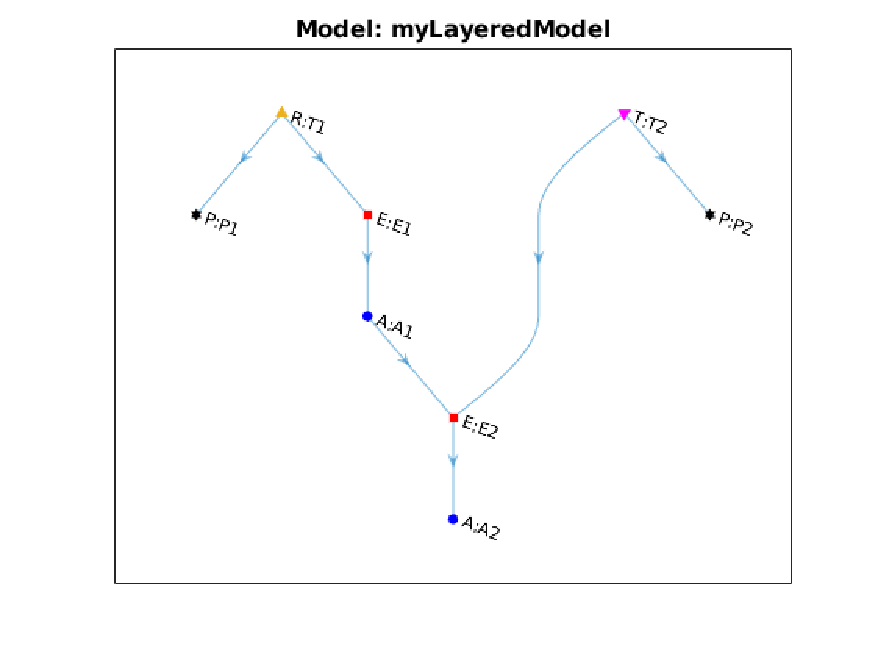
\includegraphics[width=8cm]{./images/lqnView.pdf}
  \caption{\texttt{LayeredNetwork.plot} method}\label{FIG_lqnView}
\end{figure}

When invoked as

\begin{lstlisting}[language = matlab]
plot(model,true)
\end{lstlisting}
\end{MATLAB}
\begin{JAVA}
\begin{lstlisting}[language=java, basicstyle=\ttfamily\scriptsize]
model.view();
\end{lstlisting}
\end{JAVA}
\begin{KOTLIN}
\begin{lstlisting}[language=kotlin, basicstyle=\ttfamily\scriptsize]
model.view();
\end{lstlisting}
\end{KOTLIN}
\begin{PYTHON}
\begin{lstlisting}[language=python]
model.view()
\end{lstlisting}
\end{PYTHON}
%the plot is also accompanied by a task graph that illustrates the client-server dependencies between the layers.
%As in the case of the \Matlab{Network} class, the \texttt{getGraph} method can be called to inspect the structure of the \texttt{LayeredNetwork} object.

The \Matlab{\texttt{jsimgView}}\Java{\texttt{jsimgView}}\Kotlin{\texttt{jsimgView}}\Python{\texttt{jsimg\_view}} and \Matlab{\texttt{jsimwView}}\Java{\texttt{jsimwView}}\Kotlin{\texttt{jsimwView}}\Python{\texttt{jsimw\_view}} methods can be used to visualize in JMT each layer. This can be done by first calling the \Matlab{\texttt{getLayers}}\Java{\texttt{getLayers}}\Kotlin{\texttt{getLayers}}\Python{\texttt{get\_layers}} method to obtain a \Matlab{cell array}\Java{list}\Kotlin{list}\Python{list} consisting of the \Matlab{Network}\Java{Network}\Kotlin{Network}\Python{Network} objects, each one corresponding to a layer, and then invoking the \Matlab{\texttt{jsimgView}}\Java{\texttt{jsimgView}}\Kotlin{\texttt{jsimgView}}\Python{\texttt{jsimg\_view}} and \Matlab{\texttt{jsimwView}}\Java{\texttt{jsimwView}}\Kotlin{\texttt{jsimwView}}\Python{\texttt{jsimw\_view}} methods on the desired layer. This is discussed in more details in the next section.

Lastly, we note a number of specification issues that trigger errors in the LQN definition:

{\scriptsize
\begin{table}[h!]
\centering
\begin{tabular}{|p{0.45\linewidth}|p{0.45\linewidth}|}
\hline
\textbf{Error Type} & \textbf{Error Type} \\
\hline
Activity in REF task replies & Entry called both synchronously and asynchronously \\
\hline
Entry on task calls itself & Repeated definition of parent task \\
\hline
Entry on task calls entry on the same task & Invalid .on() argument for an activity \\
\hline
Cycle in activity graph & Invalid .on() argument for a task \\
\hline
Unsupported \Matlab{replyTo}\Java{replyTo}\Kotlin{replyTo}\Python{reply\_to} & Repeated synch calls \\
\hline
Activity with \Matlab{boundTo}\Java{boundTo}\Kotlin{boundTo}\Python{bound\_to} specification & Repeated asynch calls \\
\hline
\end{tabular}
\end{table}
}

\section{Internals}

\subsection{Representation of the model structure}
It is possible to access the internal representation of a \texttt{LayeredNetwork} model in a similar way as for \Matlab{Network} objects, i.e.:
\begin{MATLAB}
\begin{lstlisting}[language = matlab]
lqn = model.getStruct();
\end{lstlisting}
\end{MATLAB}
\begin{JAVA}
\begin{lstlisting}[language = java, basicstyle=\ttfamily\scriptsize]
LayeredNetworkStruct lqn = model.getStruct();
\end{lstlisting}
\end{JAVA}
\begin{KOTLIN}
\begin{lstlisting}[language = kotlin, basicstyle=\ttfamily\scriptsize]
val lqn: LayeredNetworkStruct = model.getStruct()
\end{lstlisting}
\end{KOTLIN}
\begin{PYTHON}
\begin{lstlisting}[language=python]
lqn = model.getStruct()
\end{lstlisting}
\end{PYTHON}
The return \texttt{lqn} structure, of class \texttt{LayeredNetworkStruct}, contains all the information about the specified model. It relies on relative and absolute indexing for the elements of the \texttt{LayeredNetwork}. 
\begin{itemize}
    \item A \textit{relative} index is a number between 1 and the number of similar elements in the model, e.g., for a model with 3 tasks, the relative index $t$ of a task would be a number in $[1,3]$.
    \item An \textit{absolute} index is a number between 1 and the total number of elements (of any kind, except calls) in the model, e.g., for a model with 2 hosts, 3 tasks, 5 entries, and 8 activities, the total number of elements is \texttt{nidx}$=18$ and last activity $a$ may have an absolute index \texttt{aidx}$=18$ and a relative index \texttt{a}$=8$. 
    \item The difference between the relative and the absolute index of an element is referred to as \textit{shift}, e.g., in the previous example \texttt{ashift}$=18-8=10$.
    \item Absolute and relative indexing for calls and hosts are identical, call index \texttt{cidx} ranges in $[1,\mathtt{ncalls}]$ and host index \texttt{hidx} ranges in $[1,\mathtt{nhosts}]$.
\end{itemize}
Using the above convention, the internal representation of the model is described in \Matlab{Table~\ref{TAB_LQNPAR}}\Java{Table~\ref{TAB_LQNPAR_JAR}}\Kotlin{Table~\ref{TAB_LQNPAR_JAR}}\Python{Table~\ref{TAB_LQNPAR_PYTHON}}. As in the examples above, relative and absolute indexes are differentiated by using the suffix \texttt{idx} in the latter (e.g., \texttt{a}  vs. \texttt{aidx}). This indexing style is used throughout the codebase as well.

\begin{MATLAB}

{\scriptsize
\begin{longtable}{|p{0.28\linewidth}|p{0.17\linewidth}|p{0.50\linewidth}|}
\caption{\texttt{LayeredNetworkStruct} static properties}\label{TAB_LQNPAR}\\
\hline
\textbf{Field} & \textbf{Type} & \textbf{Description} \\
\hline
\texttt{nidx} & \texttt{integer} & Total number of \texttt{LayeredNetwork} elements \\\hline
\texttt{nhosts} & \texttt{integer} & Number of \texttt{Hosts} or \texttt{Processor} elements \\\hline
\texttt{ntasks} & \texttt{integer} & Number of \texttt{Tasks} elements \\\hline
\texttt{nentries} & \texttt{integer} & Number of \texttt{Entry} elements \\\hline
\texttt{nacts} & \texttt{integer} & Number of \texttt{Activity} elements \\\hline
\texttt{ncalls} & \texttt{integer} & Number of calls issued by \texttt{Activity} elements \\\hline
\texttt{hshift} & \texttt{integer} & For host $h$, the value $h+$\texttt{hshift} returns its absolute index in $1...$\texttt{nidx} \\\hline
\texttt{tshift} & \texttt{integer} & For task $t$, the value $t+$\texttt{tshift} returns its absolute index in $1...$\texttt{nidx} \\\hline
\texttt{eshift} & \texttt{integer} & For entry $e$, the value $e+$\texttt{eshift} returns its absolute index in $1...$\texttt{nidx} \\\hline
\texttt{ashift} & \texttt{integer} & For activity $a$, the value $a+$\texttt{ashift} returns its absolute index in $1...$\texttt{nidx} \\\hline
\texttt{cshift} & \texttt{integer} & For call $c$, the value $c+$\texttt{cshift} returns its absolute index in $1...$\texttt{ncalls} \\\hline
\texttt{tasksof}$\{hidx\}$ & \texttt{array} & Array of absolute indexes for tasks on host with absolute index \textit{hidx} \\\hline
\texttt{entriesof}$\{tidx\}$ & \texttt{array} & Array of absolute indexes for entries on task with absolute index \textit{tidx} \\\hline
\texttt{actsof}$\{eidx\}$ & \texttt{array} & Array of absolute indexes for activities reachable from entry with absolute index \textit{eidx} \\\hline
\texttt{actsof}$\{tidx\}$ & \texttt{array} & Array of absolute indexes for activities on task with absolute index \textit{tidx} \\\hline
\texttt{callsof}$\{aidx\}$ & \texttt{array} & Array of absolute indexes for calls on activity with absolute index \textit{aidx} \\\hline
\texttt{hostdem}$\{idx\}$ & \texttt{object} & \textit{(Deprecated)} Object for the host demand distribution for element \textit{idx} \\\hline
\texttt{hostdem\_type}$(idx)$ & \texttt{integer} & \texttt{ProcessType} id for host demand distribution for element \textit{idx} \\\hline
\texttt{hostdem\_params}$\{idx\}$ & \texttt{array} & Parameters array for host demand distribution for element \textit{idx} \\\hline
\texttt{hostdem\_mean}$(idx)$ & \texttt{double} & Mean of host demand distribution for element \textit{idx} \\\hline
\texttt{hostdem\_scv}$(idx)$ & \texttt{double} & Squared coefficient of variation for host demand distribution for element \textit{idx} \\\hline
\texttt{hostdem\_proc}$\{idx\}$ & \texttt{cell} & Process representation (PH/MAP matrices) for host demand for element \textit{idx} \\\hline
\texttt{think}$\{idx\}$ & \texttt{object} & \textit{(Deprecated)} Object for the think time distribution for element \textit{idx} \\\hline
\texttt{think\_type}$(idx)$ & \texttt{integer} & \texttt{ProcessType} id for think time distribution for element \textit{idx} \\\hline
\texttt{think\_params}$\{idx\}$ & \texttt{array} & Parameters array for think time distribution for element \textit{idx} \\\hline
\texttt{think\_mean}$(idx)$ & \texttt{double} & Mean of think time distribution for element \textit{idx} \\\hline
\texttt{think\_scv}$(idx)$ & \texttt{double} & Squared coefficient of variation for think time distribution for element \textit{idx} \\\hline
\texttt{think\_proc}$\{idx\}$ & \texttt{cell} & Process representation (PH/MAP matrices) for think time for element \textit{idx} \\\hline
\texttt{actthink}$\{idx\}$ & \texttt{object} & \textit{(Deprecated)} Object for the activity think time distribution for element \textit{idx} \\\hline
\texttt{actthink\_type}$(idx)$ & \texttt{integer} & \texttt{ProcessType} id for activity think time distribution for element \textit{idx} \\\hline
\texttt{actthink\_params}$\{idx\}$ & \texttt{array} & Parameters array for activity think time distribution for element \textit{idx} \\\hline
\texttt{actthink\_mean}$(idx)$ & \texttt{double} & Mean of activity think time distribution for element \textit{idx} \\\hline
\texttt{actthink\_scv}$(idx)$ & \texttt{double} & Squared coefficient of variation for activity think time distribution for element \textit{idx} \\\hline
\texttt{actthink\_proc}$\{idx\}$ & \texttt{cell} & Process representation (PH/MAP matrices) for activity think time for element \textit{idx} \\\hline
%\texttt{sched}$\{idx\}$ & \texttt{char} & \texttt{SchedStrategy} scheduling policy for a host or task with absolute index \textit{idx} \\\hline
\texttt{sched}$(idx)$ & \texttt{integer} & \texttt{SchedStrategy} scheduling policy id for a host or task with absolute index \textit{idx} \\\hline
\texttt{names}$\{idx\}$ & \texttt{char} & Name of the element with absolute index \textit{idx} \\\hline
\texttt{hashnames}$\{idx\}$ & \texttt{char} & Same as \texttt{names}$\{idx\}$ with type prefix (``H:'' for host, ``R:'' for reference task, ``T:'' \\
 &  & for task, ``C:'' for cache task, ``E:'' for entry, ``I:'' for item entry, ``A:'' for activity) \\\hline
 \texttt{mult}$(idx)$ & \texttt{integer} & Multiplicity for a host or task with absolute index \textit{idx} \\\hline
 \texttt{repl}$(idx)$ & \texttt{integer} & Replication factor for a host or task with absolute index \textit{idx} \\\hline
 \texttt{type}$\{idx\}$ & \texttt{integer} & \texttt{LayeredNetworkElement} id for an element with absolute index \textit{idx} \\\hline
\texttt{nitems}$(idx)$ & \texttt{integer} & Total number of items in \texttt{CacheTask} or \texttt{ItemEntry} \textit{idx} \\\hline
\texttt{itemcap}$\{idx\}(l)$ & \texttt{integer} & CacheTask \textit{idx} capacity for cache list $l$ \\\hline
\texttt{replacement}$(tidx)$ & \texttt{integer} & \texttt{ReplacementPolicy} id for cache task with absolute index \textit{tidx} \\\hline
\texttt{itemproc}$(idx)$ & \texttt{object} & \textit{(Deprecated)} \texttt{DiscreteDistrib} object for for the item popularity in \texttt{ItemEntry} $idx$\\\hline
\texttt{itemproc\_type}$(idx)$ & \texttt{integer} & \texttt{ProcessType} id for item popularity distribution for element \textit{idx} \\\hline
\texttt{itemproc\_params}$\{idx\}$ & \texttt{array} & Parameters array for item popularity distribution for element \textit{idx} \\\hline
\texttt{itemproc\_mean}$(idx)$ & \texttt{double} & Mean of item popularity distribution for element \textit{idx} \\\hline
\texttt{itemproc\_scv}$(idx)$ & \texttt{double} & Squared coefficient of variation for item popularity distribution for element \textit{idx} \\\hline
\texttt{itemproc\_proc}$\{idx\}$ & \texttt{cell} & Process representation for item popularity for element \textit{idx} \\\hline
\texttt{calltype}$(cidx)$ & \texttt{integer} & \texttt{CallType} id for call \textit{cidx}\\\hline
\texttt{callpair}$(cidx,j)$ & \texttt{integer} & $j=1$ is the activity \textit{aidx} issuing call \textit{cidx}, $j=2$ is the entry \textit{eidx} called by \textit{cidx} \\\hline
\texttt{callproc}$(cidx)$ & \texttt{object} & \textit{(Deprecated)} \texttt{DiscreteDistrib} object for the number of calls with absolute index \textit{cidx}\\\hline
\texttt{callproc\_type}$(cidx)$ & \texttt{integer} & \texttt{ProcessType} id for call count distribution for call \textit{cidx} \\\hline
\texttt{callproc\_params}$\{cidx\}$ & \texttt{array} & Parameters array for call count distribution for call \textit{cidx} \\\hline
\texttt{callproc\_mean}$(cidx)$ & \texttt{double} & Mean of call count distribution for call \textit{cidx} \\\hline
\texttt{callproc\_scv}$(cidx)$ & \texttt{double} & Squared coefficient of variation for call count distribution for call \textit{cidx} \\\hline
\texttt{callproc\_proc}$\{cidx\}$ & \texttt{cell} & Process representation for call count for call \textit{cidx} \\\hline
\texttt{callnames}$\{cidx\}$ &  \texttt{char} & Automatically assigned name to call with absolute index \textit{cidx} \\\hline
\texttt{callhashnames}$\{cidx\}$ &  \texttt{char} & Same as \texttt{callnames}$\{cidx\}$ but with type prefix for source and destination \\\hline
\texttt{actpretype}$(aidx)$ &  \texttt{integer} & \texttt{ActivityPrecedenceType} id preceding the activity with absolute index \textit{aidx} \\\hline
\texttt{actposttype}$(aidx)$ &  \texttt{integer} & \texttt{ActivityPrecedenceType} id after the activity with absolute index \textit{aidx} \\\hline
\texttt{graph}$(idx_i,idx_j)$ & \texttt{float} & $\neq 0$ if ${idx_i}$ ``runs on'', ``calls'' or ``precedes'' ${idx_j}$. Values are by default $1.0$ unless\\
  & & they specify a mean number of calls, a probability, fork fan-out or join fan-in degrees\\\hline
\texttt{dag}$(idx_i,idx_j)$ & \texttt{float} & Similar to \texttt{graph}$(idx_i,idx_j)$ but loops do not form cycles and entry-task edges are flipped direction at non-reference tasks to aid multiplicity analysis.\\  \hline
\texttt{parent}$(idx)$ & \texttt{integer} & Return absolute index value of the parent node for the node whose
absolute index value is $idx$\\\hline
\texttt{replygraph}$(aidx,eidx)$ & \texttt{logical} & True if activity with absolute index \textit{aidx} on entry \textit{eidx} replies ending the entry call\\\hline
\texttt{taskgraph}$(tidx_i,tidx_j)$ & \texttt{logical} & True if host or task $idx_i$ is a caller of host or task $idx_j$\\\hline
\texttt{iscache}$(tidx)$ &  \texttt{logical} & True if task \textit{tidx} is a \texttt{CacheTask}\\\hline
\texttt{iscaller}$(idx_i,idx_j)$ &  \texttt{logical} &True if task or activity ${idx_i}$ calls task or entry ${idx_j}$\\\hline
\texttt{issynccaller}$(idx_i,idx_j)$ &  \texttt{logical} &True if task or activity ${idx_i}$ issues a synchronous call to task or entry ${idx_j}$ \\\hline
\texttt{isasynccaller}$(idx_i,idx_j)$ &  \texttt{logical} &True if task or activity ${idx_i}$ issues an asynchronous call to task or entry ${idx_j}$ \\\hline
\texttt{isref}$(tidx)$ &  \texttt{logical} &True if task \textit{tidx} is a reference task\\\hline
\texttt{isfunction}$(tidx)$ &  \texttt{logical} &True if task \textit{tidx} is a function task\\\hline
\texttt{setuptime}$\{idx\}$ & \texttt{object} & \textit{(Deprecated)} Object for the setup time distribution for element \textit{idx} \\\hline
\texttt{setuptime\_type}$(idx)$ & \texttt{integer} & \texttt{ProcessType} id for setup time distribution for element \textit{idx} \\\hline
\texttt{setuptime\_params}$\{idx\}$ & \texttt{array} & Parameters array for setup time distribution for element \textit{idx} \\\hline
\texttt{setuptime\_mean}$(idx)$ & \texttt{double} & Mean of setup time distribution for element \textit{idx} \\\hline
\texttt{setuptime\_scv}$(idx)$ & \texttt{double} & Squared coefficient of variation for setup time distribution for element \textit{idx} \\\hline
\texttt{setuptime\_proc}$\{idx\}$ & \texttt{cell} & Process representation (PH/MAP matrices) for setup time for element \textit{idx} \\\hline
\texttt{delayofftime}$\{idx\}$ & \texttt{object} & \textit{(Deprecated)} Object for the delay-off time distribution for element \textit{idx} \\\hline
\texttt{delayofftime\_type}$(idx)$ & \texttt{integer} & \texttt{ProcessType} id for delay-off time distribution for element \textit{idx} \\\hline
\texttt{delayofftime\_params}$\{idx\}$ & \texttt{array} & Parameters array for delay-off time distribution for element \textit{idx} \\\hline
\texttt{delayofftime\_mean}$(idx)$ & \texttt{double} & Mean of delay-off time distribution for element \textit{idx} \\\hline
\texttt{delayofftime\_scv}$(idx)$ & \texttt{double} & Squared coefficient of variation for delay-off time distribution for element \textit{idx} \\\hline
\texttt{delayofftime\_proc}$\{idx\}$ & \texttt{cell} & Process representation (PH/MAP matrices) for delay-off time for element \textit{idx} \\\hline
\texttt{arrival}$\{eidx\}$ & \texttt{object} & \textit{(Deprecated)} Object for open arrival distribution for entry \textit{eidx} \\\hline
\texttt{arrival\_type}$(eidx)$ & \texttt{integer} & \texttt{ProcessType} id for arrival distribution for entry \textit{eidx} \\\hline
\texttt{arrival\_params}$\{eidx\}$ & \texttt{array} & Parameters array for arrival distribution for entry \textit{eidx} \\\hline
\texttt{arrival\_mean}$(eidx)$ & \texttt{double} & Mean of arrival distribution for entry \textit{eidx} \\\hline
\texttt{arrival\_scv}$(eidx)$ & \texttt{double} & Squared coefficient of variation for arrival distribution for entry \textit{eidx} \\\hline
\texttt{arrival\_proc}$\{eidx\}$ & \texttt{cell} & Process representation (PH/MAP matrices) for arrival for entry \textit{eidx} \\\hline
\end{longtable}
}

\end{MATLAB}
\begin{JAVA}
The \texttt{LayeredNetworkStruct} class in the JAR version provides the internal representation using Java/Kotlin data structures. Table~\ref{TAB_LQNPAR_JAR} lists the main properties available.
\begin{KOTLIN}
The \texttt{LayeredNetworkStruct} class provides idiomatic Kotlin access to the internal representation with improved type safety and nullable annotations. Table~\ref{TAB_LQNPAR_JAR} lists the main properties available in the Kotlin API.
\end{KOTLIN}

{\scriptsize
\begin{longtable}{|p{0.28\linewidth}|p{0.17\linewidth}|p{0.50\linewidth}|}
\caption{\texttt{LayeredNetworkStruct} static properties (JAR version)}\label{TAB_LQNPAR_JAR}\\
\hline
\textbf{Field} & \textbf{Type} & \textbf{Description} \\
\hline
\endfirsthead
\multicolumn{3}{c}{\tablename\ \thetable\ -- \textit{Continued from previous page}} \\
\hline
\textbf{Field} & \textbf{Type} & \textbf{Description} \\
\hline
\endhead
\hline \multicolumn{3}{r}{\textit{Continued on next page}} \\
\endfoot
\hline
\endlastfoot
\texttt{nidx} & \texttt{int} & Total number of \texttt{LayeredNetwork} elements\\\hline
\texttt{nhosts} & \texttt{int} & Number of \texttt{Hosts} or \texttt{Processor} elements\\\hline
\texttt{ntasks} & \texttt{int} & Number of \texttt{Tasks} elements\\\hline
\texttt{nentries} & \texttt{int} & Number of \texttt{Entry} elements\\\hline
\texttt{nacts} & \texttt{int} & Number of \texttt{Activity} elements\\\hline
\texttt{ncalls} & \texttt{int} & Number of calls issued by \texttt{Activity} elements\\\hline
\texttt{hshift} & \texttt{int} & For host $h$, the value $h+$\texttt{hshift} returns its absolute index in $1...$\texttt{nidx}\\\hline
\texttt{tshift} & \texttt{int} & For task $t$, the value $t+$\texttt{tshift} returns its absolute index in $1...$\texttt{nidx}\\\hline
\texttt{eshift} & \texttt{int} & For entry $e$, the value $e+$\texttt{eshift} returns its absolute index in $1...$\texttt{nidx}\\\hline
\texttt{ashift} & \texttt{int} & For activity $a$, the value $a+$\texttt{ashift} returns its absolute index in $1...$\texttt{nidx}\\\hline
\texttt{cshift} & \texttt{int} & For call $c$, the value $c+$\texttt{cshift} returns its absolute index in $1...$\texttt{ncalls}\\\hline
\texttt{tasksof} & \texttt{Map\textlangle Integer, List\textlangle Integer\textrangle\textrangle} & Map from host absolute index to list of task absolute indexes on that host\\\hline
\texttt{entriesof} & \texttt{Map\textlangle Integer, List\textlangle Integer\textrangle\textrangle} & Map from task absolute index to list of entry absolute indexes on that task\\\hline
\texttt{actsof} & \texttt{Map\textlangle Integer, List\textlangle Integer\textrangle\textrangle} & Map from entry/task absolute index to list of activity absolute indexes\\\hline
\texttt{callsof} & \texttt{Map\textlangle Integer, List\textlangle Integer\textrangle\textrangle} & Map from activity absolute index to list of call absolute indexes\\\hline
\texttt{hostdem} & \texttt{Map\textlangle Integer, Distribution\textrangle} & \textit{(Deprecated)} Host demand distribution for each element by absolute index\\\hline
\texttt{hostdem\_type} & \texttt{Map\textlangle Integer, ProcessType\textrangle} & Host demand distribution type by absolute index\\\hline
\texttt{hostdem\_params} & \texttt{Map\textlangle Integer, Matrix\textrangle} & Host demand distribution parameters by absolute index\\\hline
\texttt{hostdem\_mean} & \texttt{Map\textlangle Integer, Double\textrangle} & Host demand mean by absolute index\\\hline
\texttt{hostdem\_scv} & \texttt{Map\textlangle Integer, Double\textrangle} & Host demand squared coefficient of variation by absolute index\\\hline
\texttt{hostdem\_proc} & \texttt{Map\textlangle Integer, MatrixCell\textrangle} & Host demand process representation (PH/MAP) by absolute index\\\hline
\texttt{think} & \texttt{Map\textlangle Integer, Distribution\textrangle} & \textit{(Deprecated)} Think time distribution for each element by absolute index\\\hline
\texttt{think\_type} & \texttt{Map\textlangle Integer, ProcessType\textrangle} & Think time distribution type by absolute index\\\hline
\texttt{think\_params} & \texttt{Map\textlangle Integer, Matrix\textrangle} & Think time distribution parameters by absolute index\\\hline
\texttt{think\_mean} & \texttt{Map\textlangle Integer, Double\textrangle} & Think time mean by absolute index\\\hline
\texttt{think\_scv} & \texttt{Map\textlangle Integer, Double\textrangle} & Think time squared coefficient of variation by absolute index\\\hline
\texttt{think\_proc} & \texttt{Map\textlangle Integer, MatrixCell\textrangle} & Think time process representation (PH/MAP) by absolute index\\\hline
\texttt{actthink} & \texttt{Map\textlangle Integer, Distribution\textrangle} & \textit{(Deprecated)} Activity think time distribution by absolute index\\\hline
\texttt{actthink\_type} & \texttt{Map\textlangle Integer, ProcessType\textrangle} & Activity think time distribution type by absolute index\\\hline
\texttt{actthink\_params} & \texttt{Map\textlangle Integer, Matrix\textrangle} & Activity think time distribution parameters by absolute index\\\hline
\texttt{actthink\_mean} & \texttt{Map\textlangle Integer, Double\textrangle} & Activity think time mean by absolute index\\\hline
\texttt{actthink\_scv} & \texttt{Map\textlangle Integer, Double\textrangle} & Activity think time squared coefficient of variation by absolute index\\\hline
\texttt{actthink\_proc} & \texttt{Map\textlangle Integer, MatrixCell\textrangle} & Activity think time process representation (PH/MAP) by absolute index\\\hline
\texttt{sched} & \texttt{Map\textlangle Integer, SchedStrategy\textrangle} & Scheduling strategy for host or task by absolute index\\\hline
\texttt{names} & \texttt{Map\textlangle Integer, String\textrangle} & Name of element by absolute index\\\hline
\texttt{hashnames} & \texttt{Map\textlangle Integer, String\textrangle} & Name with type prefix by absolute index (``H:'' host, ``R:'' reference task, ``T:'' task, ``C:'' cache task, ``E:'' entry, ``I:'' item entry, ``A:'' activity)\\\hline
\texttt{mult} & \texttt{Matrix} & Multiplicity for host or task by absolute index\\\hline
\texttt{maxmult} & \texttt{Matrix} & Maximum multiplicity for host or task by absolute index\\\hline
\texttt{repl} & \texttt{Matrix} & Replication factor for host or task by absolute index\\\hline
\texttt{type} & \texttt{Matrix} & \texttt{LayeredNetworkElement} type id for element by absolute index\\\hline
\texttt{nitems} & \texttt{Matrix} & Number of items in \texttt{CacheTask} or \texttt{ItemEntry} by absolute index\\\hline
\texttt{itemcap} & \texttt{Map\textlangle Integer, Integer\textrangle} & Cache capacity for cache list by absolute index\\\hline
\texttt{replacestrat} & \texttt{Matrix} & \texttt{ReplacementStrategy} id for cache task by absolute index\\\hline
\texttt{itemproc} & \texttt{Map\textlangle Integer, DiscreteDistribution\textrangle} & \textit{(Deprecated)} Item popularity distribution for \texttt{ItemEntry} by absolute index\\\hline
\texttt{itemproc\_type} & \texttt{Map\textlangle Integer, ProcessType\textrangle} & Item popularity distribution type by absolute index\\\hline
\texttt{itemproc\_params} & \texttt{Map\textlangle Integer, Matrix\textrangle} & Item popularity distribution parameters by absolute index\\\hline
\texttt{itemproc\_mean} & \texttt{Map\textlangle Integer, Double\textrangle} & Item popularity mean by absolute index\\\hline
\texttt{itemproc\_scv} & \texttt{Map\textlangle Integer, Double\textrangle} & Item popularity squared coefficient of variation by absolute index\\\hline
\texttt{itemproc\_proc} & \texttt{Map\textlangle Integer, MatrixCell\textrangle} & Item popularity process representation by absolute index\\\hline
\texttt{calltype} & \texttt{Map\textlangle Integer, CallType\textrangle} & \texttt{CallType} for call by call index\\\hline
\texttt{callpair} & \texttt{Matrix} & Call relationship matrix: column 1 = activity issuing call, column 2 = entry being called\\\hline
\texttt{callproc} & \texttt{Map\textlangle Integer, DiscreteDistribution\textrangle} & \textit{(Deprecated)} Number of calls distribution by call absolute index\\\hline
\texttt{callproc\_type} & \texttt{Map\textlangle Integer, ProcessType\textrangle} & Call count distribution type by call absolute index\\\hline
\texttt{callproc\_params} & \texttt{Map\textlangle Integer, Matrix\textrangle} & Call count distribution parameters by call absolute index\\\hline
\texttt{callproc\_mean} & \texttt{Map\textlangle Integer, Double\textrangle} & Call count mean by call absolute index\\\hline
\texttt{callproc\_scv} & \texttt{Map\textlangle Integer, Double\textrangle} & Call count squared coefficient of variation by call absolute index\\\hline
\texttt{callproc\_proc} & \texttt{Map\textlangle Integer, MatrixCell\textrangle} & Call count process representation by call absolute index\\\hline
\texttt{callnames} & \texttt{Map\textlangle Integer, String\textrangle} & Name of call by call absolute index\\\hline
\texttt{callhashnames} & \texttt{Map\textlangle Integer, String\textrangle} & Call name with type prefixes for source and destination\\\hline
\texttt{actpretype} & \texttt{Matrix} & \texttt{ActivityPrecedenceType} id before activity by absolute index\\\hline
\texttt{actposttype} & \texttt{Matrix} & \texttt{ActivityPrecedenceType} id after activity by absolute index\\\hline
\texttt{graph} & \texttt{Matrix} & Adjacency matrix: $\neq 0$ if element $i$ ``runs on'', ``calls'' or ``precedes'' element $j$\\\hline
\texttt{dag} & \texttt{Matrix} & Directed acyclic graph version of \texttt{graph} with flipped entry-task edges\\\hline
\texttt{parent} & \texttt{Matrix} & Parent element absolute index for each element\\\hline
\texttt{replygraph} & \texttt{Matrix} & True if activity replies, ending the entry call\\\hline
\texttt{taskgraph} & \texttt{Matrix} & True if host/task $i$ calls host/task $j$\\\hline
\texttt{iscache} & \texttt{Matrix} & True if task is a \texttt{CacheTask}\\\hline
\texttt{iscaller} & \texttt{Matrix} & True if element $i$ calls element $j$\\\hline
\texttt{issynccaller} & \texttt{Matrix} & True if element $i$ issues synchronous call to element $j$\\\hline
\texttt{isasynccaller} & \texttt{Matrix} & True if element $i$ issues asynchronous call to element $j$\\\hline
\texttt{isref} & \texttt{Matrix} & True if task is a reference task\\\hline
\texttt{isfunction} & \texttt{Matrix} & True if task is a function task\\\hline
\texttt{setuptime} & \texttt{Map\textlangle Integer, Distribution\textrangle} & \textit{(Deprecated)} Setup time distribution by absolute index\\\hline
\texttt{setuptime\_type} & \texttt{Map\textlangle Integer, ProcessType\textrangle} & Setup time distribution type by absolute index\\\hline
\texttt{setuptime\_params} & \texttt{Map\textlangle Integer, Matrix\textrangle} & Setup time distribution parameters by absolute index\\\hline
\texttt{setuptime\_mean} & \texttt{Map\textlangle Integer, Double\textrangle} & Setup time mean by absolute index\\\hline
\texttt{setuptime\_scv} & \texttt{Map\textlangle Integer, Double\textrangle} & Setup time squared coefficient of variation by absolute index\\\hline
\texttt{setuptime\_proc} & \texttt{Map\textlangle Integer, MatrixCell\textrangle} & Setup time process representation (PH/MAP) by absolute index\\\hline
\texttt{delayofftime} & \texttt{Map\textlangle Integer, Distribution\textrangle} & \textit{(Deprecated)} Delay-off time distribution by absolute index\\\hline
\texttt{delayofftime\_type} & \texttt{Map\textlangle Integer, ProcessType\textrangle} & Delay-off time distribution type by absolute index\\\hline
\texttt{delayofftime\_params} & \texttt{Map\textlangle Integer, Matrix\textrangle} & Delay-off time distribution parameters by absolute index\\\hline
\texttt{delayofftime\_mean} & \texttt{Map\textlangle Integer, Double\textrangle} & Delay-off time mean by absolute index\\\hline
\texttt{delayofftime\_scv} & \texttt{Map\textlangle Integer, Double\textrangle} & Delay-off time squared coefficient of variation by absolute index\\\hline
\texttt{delayofftime\_proc} & \texttt{Map\textlangle Integer, MatrixCell\textrangle} & Delay-off time process representation (PH/MAP) by absolute index\\\hline
\texttt{arrival} & \texttt{Map\textlangle Integer, Distribution\textrangle} & \textit{(Deprecated)} Open arrival distribution for entries by absolute index\\\hline
\texttt{arrival\_type} & \texttt{Map\textlangle Integer, ProcessType\textrangle} & Arrival distribution type by absolute index\\\hline
\texttt{arrival\_params} & \texttt{Map\textlangle Integer, Matrix\textrangle} & Arrival distribution parameters by absolute index\\\hline
\texttt{arrival\_mean} & \texttt{Map\textlangle Integer, Double\textrangle} & Arrival mean by absolute index\\\hline
\texttt{arrival\_scv} & \texttt{Map\textlangle Integer, Double\textrangle} & Arrival squared coefficient of variation by absolute index\\\hline
\texttt{arrival\_proc} & \texttt{Map\textlangle Integer, MatrixCell\textrangle} & Arrival process representation (PH/MAP) by absolute index\\\hline
\texttt{conntasks} & \texttt{Matrix} & Connected tasks matrix\\\hline
\texttt{hitmissaidx} & \texttt{List\textlangle Integer\textrangle} & List of hit/miss activity absolute indexes\\\hline
\texttt{hitaidx} & \texttt{Integer} & Hit activity absolute index\\\hline
\texttt{missaidx} & \texttt{Integer} & Miss activity absolute index\\\hline
\end{longtable}
}
\end{JAVA}
\begin{KOTLIN}
The \texttt{LayeredNetworkStruct} class provides idiomatic Kotlin access to the internal representation with improved type safety and nullable annotations. Table~\ref{TAB_LQNPAR_JAR} lists the main properties available in the Kotlin API.

{\scriptsize
\begin{longtable}{|p{0.28\linewidth}|p{0.17\linewidth}|p{0.50\linewidth}|}
\caption{\texttt{LayeredNetworkStruct} static properties (JAR version)}\label{TAB_LQNPAR_JAR}\\
\hline
\textbf{Field} & \textbf{Type} & \textbf{Description} \\
\hline
\endfirsthead
\multicolumn{3}{c}{\tablename\ \thetable\ -- \textit{Continued from previous page}} \\
\hline
\textbf{Field} & \textbf{Type} & \textbf{Description} \\
\hline
\endhead
\hline \multicolumn{3}{r}{\textit{Continued on next page}} \\
\endfoot
\hline
\endlastfoot
\texttt{nidx} & \texttt{int} & Total number of \texttt{LayeredNetwork} elements\\\hline
\texttt{nhosts} & \texttt{int} & Number of \texttt{Hosts} or \texttt{Processor} elements\\\hline
\texttt{ntasks} & \texttt{int} & Number of \texttt{Tasks} elements\\\hline
\texttt{nentries} & \texttt{int} & Number of \texttt{Entry} elements\\\hline
\texttt{nacts} & \texttt{int} & Number of \texttt{Activity} elements\\\hline
\texttt{ncalls} & \texttt{int} & Number of calls issued by \texttt{Activity} elements\\\hline
\texttt{hshift} & \texttt{int} & For host $h$, the value $h+$\texttt{hshift} returns its absolute index in $1...$\texttt{nidx}\\\hline
\texttt{tshift} & \texttt{int} & For task $t$, the value $t+$\texttt{tshift} returns its absolute index in $1...$\texttt{nidx}\\\hline
\texttt{eshift} & \texttt{int} & For entry $e$, the value $e+$\texttt{eshift} returns its absolute index in $1...$\texttt{nidx}\\\hline
\texttt{ashift} & \texttt{int} & For activity $a$, the value $a+$\texttt{ashift} returns its absolute index in $1...$\texttt{nidx}\\\hline
\texttt{cshift} & \texttt{int} & For call $c$, the value $c+$\texttt{cshift} returns its absolute index in $1...$\texttt{ncalls}\\\hline
\texttt{tasksof} & \texttt{Map\textlangle Integer, List\textlangle Integer\textrangle\textrangle} & Map from host absolute index to list of task absolute indexes on that host\\\hline
\texttt{entriesof} & \texttt{Map\textlangle Integer, List\textlangle Integer\textrangle\textrangle} & Map from task absolute index to list of entry absolute indexes on that task\\\hline
\texttt{actsof} & \texttt{Map\textlangle Integer, List\textlangle Integer\textrangle\textrangle} & Map from entry/task absolute index to list of activity absolute indexes\\\hline
\texttt{callsof} & \texttt{Map\textlangle Integer, List\textlangle Integer\textrangle\textrangle} & Map from activity absolute index to list of call absolute indexes\\\hline
\texttt{hostdem} & \texttt{Map\textlangle Integer, Distribution\textrangle} & \textit{(Deprecated)} Host demand distribution for each element by absolute index\\\hline
\texttt{hostdem\_type} & \texttt{Map\textlangle Integer, ProcessType\textrangle} & Host demand distribution type by absolute index\\\hline
\texttt{hostdem\_params} & \texttt{Map\textlangle Integer, Matrix\textrangle} & Host demand distribution parameters by absolute index\\\hline
\texttt{hostdem\_mean} & \texttt{Map\textlangle Integer, Double\textrangle} & Host demand mean by absolute index\\\hline
\texttt{hostdem\_scv} & \texttt{Map\textlangle Integer, Double\textrangle} & Host demand squared coefficient of variation by absolute index\\\hline
\texttt{hostdem\_proc} & \texttt{Map\textlangle Integer, MatrixCell\textrangle} & Host demand process representation (PH/MAP) by absolute index\\\hline
\texttt{think} & \texttt{Map\textlangle Integer, Distribution\textrangle} & \textit{(Deprecated)} Think time distribution for each element by absolute index\\\hline
\texttt{think\_type} & \texttt{Map\textlangle Integer, ProcessType\textrangle} & Think time distribution type by absolute index\\\hline
\texttt{think\_params} & \texttt{Map\textlangle Integer, Matrix\textrangle} & Think time distribution parameters by absolute index\\\hline
\texttt{think\_mean} & \texttt{Map\textlangle Integer, Double\textrangle} & Think time mean by absolute index\\\hline
\texttt{think\_scv} & \texttt{Map\textlangle Integer, Double\textrangle} & Think time squared coefficient of variation by absolute index\\\hline
\texttt{think\_proc} & \texttt{Map\textlangle Integer, MatrixCell\textrangle} & Think time process representation (PH/MAP) by absolute index\\\hline
\texttt{actthink} & \texttt{Map\textlangle Integer, Distribution\textrangle} & \textit{(Deprecated)} Activity think time distribution by absolute index\\\hline
\texttt{actthink\_type} & \texttt{Map\textlangle Integer, ProcessType\textrangle} & Activity think time distribution type by absolute index\\\hline
\texttt{actthink\_params} & \texttt{Map\textlangle Integer, Matrix\textrangle} & Activity think time distribution parameters by absolute index\\\hline
\texttt{actthink\_mean} & \texttt{Map\textlangle Integer, Double\textrangle} & Activity think time mean by absolute index\\\hline
\texttt{actthink\_scv} & \texttt{Map\textlangle Integer, Double\textrangle} & Activity think time squared coefficient of variation by absolute index\\\hline
\texttt{actthink\_proc} & \texttt{Map\textlangle Integer, MatrixCell\textrangle} & Activity think time process representation (PH/MAP) by absolute index\\\hline
\texttt{sched} & \texttt{Map\textlangle Integer, SchedStrategy\textrangle} & Scheduling strategy for host or task by absolute index\\\hline
\texttt{names} & \texttt{Map\textlangle Integer, String\textrangle} & Name of element by absolute index\\\hline
\texttt{hashnames} & \texttt{Map\textlangle Integer, String\textrangle} & Name with type prefix by absolute index (``H:'' host, ``R:'' reference task, ``T:'' task, ``C:'' cache task, ``E:'' entry, ``I:'' item entry, ``A:'' activity)\\\hline
\texttt{mult} & \texttt{Matrix} & Multiplicity for host or task by absolute index\\\hline
\texttt{maxmult} & \texttt{Matrix} & Maximum multiplicity for host or task by absolute index\\\hline
\texttt{repl} & \texttt{Matrix} & Replication factor for host or task by absolute index\\\hline
\texttt{type} & \texttt{Matrix} & \texttt{LayeredNetworkElement} type id for element by absolute index\\\hline
\texttt{nitems} & \texttt{Matrix} & Number of items in \texttt{CacheTask} or \texttt{ItemEntry} by absolute index\\\hline
\texttt{itemcap} & \texttt{Map\textlangle Integer, Integer\textrangle} & Cache capacity for cache list by absolute index\\\hline
\texttt{replacestrat} & \texttt{Matrix} & \texttt{ReplacementStrategy} id for cache task by absolute index\\\hline
\texttt{itemproc} & \texttt{Map\textlangle Integer, DiscreteDistribution\textrangle} & \textit{(Deprecated)} Item popularity distribution for \texttt{ItemEntry} by absolute index\\\hline
\texttt{itemproc\_type} & \texttt{Map\textlangle Integer, ProcessType\textrangle} & Item popularity distribution type by absolute index\\\hline
\texttt{itemproc\_params} & \texttt{Map\textlangle Integer, Matrix\textrangle} & Item popularity distribution parameters by absolute index\\\hline
\texttt{itemproc\_mean} & \texttt{Map\textlangle Integer, Double\textrangle} & Item popularity mean by absolute index\\\hline
\texttt{itemproc\_scv} & \texttt{Map\textlangle Integer, Double\textrangle} & Item popularity squared coefficient of variation by absolute index\\\hline
\texttt{itemproc\_proc} & \texttt{Map\textlangle Integer, MatrixCell\textrangle} & Item popularity process representation by absolute index\\\hline
\texttt{calltype} & \texttt{Map\textlangle Integer, CallType\textrangle} & \texttt{CallType} for call by call index\\\hline
\texttt{callpair} & \texttt{Matrix} & Call relationship matrix: column 1 = activity issuing call, column 2 = entry being called\\\hline
\texttt{callproc} & \texttt{Map\textlangle Integer, DiscreteDistribution\textrangle} & \textit{(Deprecated)} Number of calls distribution by call absolute index\\\hline
\texttt{callproc\_type} & \texttt{Map\textlangle Integer, ProcessType\textrangle} & Call count distribution type by call absolute index\\\hline
\texttt{callproc\_params} & \texttt{Map\textlangle Integer, Matrix\textrangle} & Call count distribution parameters by call absolute index\\\hline
\texttt{callproc\_mean} & \texttt{Map\textlangle Integer, Double\textrangle} & Call count mean by call absolute index\\\hline
\texttt{callproc\_scv} & \texttt{Map\textlangle Integer, Double\textrangle} & Call count squared coefficient of variation by call absolute index\\\hline
\texttt{callproc\_proc} & \texttt{Map\textlangle Integer, MatrixCell\textrangle} & Call count process representation by call absolute index\\\hline
\texttt{callnames} & \texttt{Map\textlangle Integer, String\textrangle} & Name of call by call absolute index\\\hline
\texttt{callhashnames} & \texttt{Map\textlangle Integer, String\textrangle} & Call name with type prefixes for source and destination\\\hline
\texttt{actpretype} & \texttt{Matrix} & \texttt{ActivityPrecedenceType} id before activity by absolute index\\\hline
\texttt{actposttype} & \texttt{Matrix} & \texttt{ActivityPrecedenceType} id after activity by absolute index\\\hline
\texttt{graph} & \texttt{Matrix} & Adjacency matrix: $\neq 0$ if element $i$ ``runs on'', ``calls'' or ``precedes'' element $j$\\\hline
\texttt{dag} & \texttt{Matrix} & Directed acyclic graph version of \texttt{graph} with flipped entry-task edges\\\hline
\texttt{parent} & \texttt{Matrix} & Parent element absolute index for each element\\\hline
\texttt{replygraph} & \texttt{Matrix} & True if activity replies, ending the entry call\\\hline
\texttt{taskgraph} & \texttt{Matrix} & True if host/task $i$ calls host/task $j$\\\hline
\texttt{iscache} & \texttt{Matrix} & True if task is a \texttt{CacheTask}\\\hline
\texttt{iscaller} & \texttt{Matrix} & True if element $i$ calls element $j$\\\hline
\texttt{issynccaller} & \texttt{Matrix} & True if element $i$ issues synchronous call to element $j$\\\hline
\texttt{isasynccaller} & \texttt{Matrix} & True if element $i$ issues asynchronous call to element $j$\\\hline
\texttt{isref} & \texttt{Matrix} & True if task is a reference task\\\hline
\texttt{isfunction} & \texttt{Matrix} & True if task is a function task\\\hline
\texttt{setuptime} & \texttt{Map\textlangle Integer, Distribution\textrangle} & \textit{(Deprecated)} Setup time distribution by absolute index\\\hline
\texttt{setuptime\_type} & \texttt{Map\textlangle Integer, ProcessType\textrangle} & Setup time distribution type by absolute index\\\hline
\texttt{setuptime\_params} & \texttt{Map\textlangle Integer, Matrix\textrangle} & Setup time distribution parameters by absolute index\\\hline
\texttt{setuptime\_mean} & \texttt{Map\textlangle Integer, Double\textrangle} & Setup time mean by absolute index\\\hline
\texttt{setuptime\_scv} & \texttt{Map\textlangle Integer, Double\textrangle} & Setup time squared coefficient of variation by absolute index\\\hline
\texttt{setuptime\_proc} & \texttt{Map\textlangle Integer, MatrixCell\textrangle} & Setup time process representation (PH/MAP) by absolute index\\\hline
\texttt{delayofftime} & \texttt{Map\textlangle Integer, Distribution\textrangle} & \textit{(Deprecated)} Delay-off time distribution by absolute index\\\hline
\texttt{delayofftime\_type} & \texttt{Map\textlangle Integer, ProcessType\textrangle} & Delay-off time distribution type by absolute index\\\hline
\texttt{delayofftime\_params} & \texttt{Map\textlangle Integer, Matrix\textrangle} & Delay-off time distribution parameters by absolute index\\\hline
\texttt{delayofftime\_mean} & \texttt{Map\textlangle Integer, Double\textrangle} & Delay-off time mean by absolute index\\\hline
\texttt{delayofftime\_scv} & \texttt{Map\textlangle Integer, Double\textrangle} & Delay-off time squared coefficient of variation by absolute index\\\hline
\texttt{delayofftime\_proc} & \texttt{Map\textlangle Integer, MatrixCell\textrangle} & Delay-off time process representation (PH/MAP) by absolute index\\\hline
\texttt{arrival} & \texttt{Map\textlangle Integer, Distribution\textrangle} & \textit{(Deprecated)} Open arrival distribution for entries by absolute index\\\hline
\texttt{arrival\_type} & \texttt{Map\textlangle Integer, ProcessType\textrangle} & Arrival distribution type by absolute index\\\hline
\texttt{arrival\_params} & \texttt{Map\textlangle Integer, Matrix\textrangle} & Arrival distribution parameters by absolute index\\\hline
\texttt{arrival\_mean} & \texttt{Map\textlangle Integer, Double\textrangle} & Arrival mean by absolute index\\\hline
\texttt{arrival\_scv} & \texttt{Map\textlangle Integer, Double\textrangle} & Arrival squared coefficient of variation by absolute index\\\hline
\texttt{arrival\_proc} & \texttt{Map\textlangle Integer, MatrixCell\textrangle} & Arrival process representation (PH/MAP) by absolute index\\\hline
\texttt{conntasks} & \texttt{Matrix} & Connected tasks matrix\\\hline
\texttt{hitmissaidx} & \texttt{List\textlangle Integer\textrangle} & List of hit/miss activity absolute indexes\\\hline
\texttt{hitaidx} & \texttt{Integer} & Hit activity absolute index\\\hline
\texttt{missaidx} & \texttt{Integer} & Miss activity absolute index\\\hline
\end{longtable}
}
\end{KOTLIN}
\begin{PYTHON}
The Python \texttt{LayeredNetworkStruct} provides a wrapper around the JAR implementation, converting data structures to Python-native types. Table~\ref{TAB_LQNPAR_PYTHON} lists the properties available through the Python interface.

{\scriptsize
\begin{longtable}{|p{0.28\linewidth}|p{0.17\linewidth}|p{0.50\linewidth}|}
\caption{\texttt{LayeredNetworkStruct} static properties (Python version)}\label{TAB_LQNPAR_PYTHON}\\
\hline
\textbf{Field} & \textbf{Type} & \textbf{Description} \\
\hline
\endfirsthead
\multicolumn{3}{c}{\tablename\ \thetable\ -- \textit{Continued from previous page}} \\
\hline
\textbf{Field} & \textbf{Type} & \textbf{Description} \\
\hline
\endhead
\hline \multicolumn{3}{r}{\textit{Continued on next page}} \\
\endfoot
\hline
\endlastfoot
\texttt{nidx} & \texttt{int} & Total number of \texttt{LayeredNetwork} elements\\\hline
\texttt{nhosts} & \texttt{int} & Number of \texttt{Hosts} or \texttt{Processor} elements\\\hline
\texttt{ntasks} & \texttt{int} & Number of \texttt{Tasks} elements\\\hline
\texttt{nentries} & \texttt{int} & Number of \texttt{Entry} elements\\\hline
\texttt{nacts} & \texttt{int} & Number of \texttt{Activity} elements\\\hline
\texttt{ncalls} & \texttt{int} & Number of calls issued by \texttt{Activity} elements\\\hline
\texttt{hshift} & \texttt{int} & For host $h$, the value $h+$\texttt{hshift} returns its absolute index in $1...$\texttt{nidx}\\\hline
\texttt{tshift} & \texttt{int} & For task $t$, the value $t+$\texttt{tshift} returns its absolute index in $1...$\texttt{nidx}\\\hline
\texttt{eshift} & \texttt{int} & For entry $e$, the value $e+$\texttt{eshift} returns its absolute index in $1...$\texttt{nidx}\\\hline
\texttt{ashift} & \texttt{int} & For activity $a$, the value $a+$\texttt{ashift} returns its absolute index in $1...$\texttt{nidx}\\\hline
\texttt{cshift} & \texttt{int} & For call $c$, the value $c+$\texttt{cshift} returns its absolute index in $1...$\texttt{ncalls}\\\hline
\texttt{tasksof} & numpy.ndarray & Array of lists: each element contains task absolute indexes for corresponding host (dtype=object)\\\hline
\texttt{entriesof} & numpy.ndarray & Array of lists: each element contains entry absolute indexes for corresponding task (dtype=object)\\\hline
\texttt{actsof} & numpy.ndarray & Array of lists: each element contains activity absolute indexes for corresponding entry/task (dtype=object)\\\hline
\texttt{callsof} & numpy.ndarray & Array of lists: each element contains call absolute indexes for corresponding activity (dtype=object)\\\hline
\texttt{hostdem} & numpy.ndarray & Array of distribution objects for host demand by absolute index (dtype=object)\\\hline
\texttt{think} & numpy.ndarray & Array of distribution objects for think time by absolute index (dtype=object)\\\hline
\texttt{sched} & numpy.ndarray & Array of scheduling strategy names by absolute index (dtype=object, contains strings)\\\hline
\texttt{names} & numpy.ndarray & Array of element names by absolute index (dtype=object, contains strings)\\\hline
\texttt{hashnames} & numpy.ndarray & Array of element names with type prefixes by absolute index (dtype=object, contains strings)\\\hline
\texttt{schedid} & numpy.ndarray & Scheduling strategy ID matrix for hosts/tasks\\\hline
\texttt{mult} & numpy.ndarray & Multiplicity matrix for hosts/tasks by absolute index\\\hline
\texttt{repl} & numpy.ndarray & Replication factor matrix for hosts/tasks by absolute index\\\hline
\texttt{type} & numpy.ndarray & Element type ID matrix by absolute index\\\hline
\texttt{nitems} & numpy.ndarray & Number of items matrix for cache tasks/item entries\\\hline
\texttt{itemcap} & numpy.ndarray & Array of cache capacities by absolute index (dtype=object)\\\hline
\texttt{replacement} & numpy.ndarray & Replacement strategy ID matrix for cache tasks\\\hline
\texttt{itemproc} & numpy.ndarray & Array of item popularity distribution objects by absolute index (dtype=object)\\\hline
\texttt{calltype} & numpy.ndarray & Array of call type names by call index (dtype=object, contains strings)\\\hline
\texttt{callpair} & numpy.ndarray & Call relationship matrix: column 1 = activity issuing call, column 2 = entry being called\\\hline
\texttt{callproc} & numpy.ndarray & Array of call count distribution objects by call absolute index (dtype=object)\\\hline
\texttt{callnames} & numpy.ndarray & Array of call names by call absolute index (dtype=object, contains strings)\\\hline
\texttt{callhashnames} & numpy.ndarray & Array of call names with type prefixes (dtype=object, contains strings)\\\hline
\texttt{actpretype} & numpy.ndarray & Activity precedence type matrix (before activity)\\\hline
\texttt{actposttype} & numpy.ndarray & Activity precedence type matrix (after activity)\\\hline
\texttt{graph} & numpy.ndarray & Adjacency matrix: $\neq 0$ if element $i$ ``runs on'', ``calls'' or ``precedes'' element $j$\\\hline
\texttt{parent} & numpy.ndarray & Parent element absolute index matrix\\\hline
\texttt{replygraph} & numpy.ndarray & Boolean matrix: True if activity replies, ending entry call\\\hline
\texttt{taskgraph} & numpy.ndarray & Boolean matrix: True if host/task $i$ calls host/task $j$\\\hline
\texttt{iscaller} & numpy.ndarray & Boolean matrix: True if element $i$ calls element $j$\\\hline
\texttt{issynccaller} & numpy.ndarray & Boolean matrix: True if element $i$ issues synchronous call to element $j$\\\hline
\texttt{isasynccaller} & numpy.ndarray & Boolean matrix: True if element $i$ issues asynchronous call to element $j$\\\hline
\texttt{isref} & numpy.ndarray & Boolean matrix: True if task is a reference task\\\hline
\end{longtable}
}
\end{PYTHON}

\subsection{Decomposition into layers}
Layers are a form of decomposition where we model the performance of one or more servers. The activity of clients not detailed in that layer is taken into account through an artificial delay station, placed in a closed loop to the servers~\cite{roli.sevc95}. This artificial delay is used to model the inter-arrival time between calls issued by that client.

The current version of \textsc{Line} adopts SRVN-type layering~\cite{lqns12}, whereby a layer corresponds to one and only one resource, either a processor or a task. 
The \texttt{getLayers} method returns a cell array consisting of the \Matlab{Network} objects corresponding to each layer
\begin{MATLAB}
\begin{lstlisting}[language = matlab]
layers = model.getLayers()
\end{lstlisting}
\end{MATLAB}
\begin{JAVA}
\begin{lstlisting}[language = java, basicstyle=\ttfamily\scriptsize]
\texttt{List\textlangle Network\textrangle} layers = model.getLayers();
\end{lstlisting}
\end{JAVA}
\begin{KOTLIN}
\begin{lstlisting}[language = kotlin, basicstyle=\ttfamily\scriptsize]
\texttt{List\textlangle Network\textrangle} layers = model.getLayers()
\end{lstlisting}
\end{KOTLIN}
\begin{PYTHON}
\begin{lstlisting}[language=python]
layers = model.get_layers()
\end{lstlisting}
\end{PYTHON}
The decomposition is performed through the \texttt{LN} solver described later.

Within each layer, classes are used to model the time a job spends in a given activity or call, with synchronous calls being modeled by classed with label including an arrow, e.g., \Matlab{\texttt{'AS1=>E3'}}\Java{\texttt{"AS1=>E3"}}\Python{\texttt{'AS1=>E3'}} is a closed class used represent synchronous calls from activity \texttt{AS1} to entry \texttt{E3}, whereas \Matlab{\texttt{'AS1->E3'}}\Java{\texttt{"AS1->E3"}}\Python{\texttt{'AS1->E3'}} denotes an asynchronous call. Artificial delays and reference nodes are modelled as a delay station named \texttt{'Clients'}, whereas the task or processor assigned to the layer is modelled as the other node in the layer.

% \subsection{Initialization and update}
% \label{initialization-and-update}
% In general, the parameters of a layer will depend on the steady-state solution of an other layer, causing a cyclic dependence that can be broken only after the model is analyzed by a solver. In order to assign parameters within each layer prior to its solution, the \texttt{LayeredNetwork} class uses the \Matlab{initDefault} method, which sets the value of the artificial delay to simple operational analysis bounds~\cite{LazZGS84}.

% The layer parameterization depends on a subset of performance indexes stored in a \texttt{param} structure array within the \texttt{LayeredNetwork} class. After initialization, it is possible to update the layer parameterization for example as follows
% \begin{lstlisting}[language = matlab]
% layers = model.getLayers();
% for l=1:model.getNumberOfLayers()
%     AvgTableByLayer{l} = MVA(layers{l}).avgTable;
% end
% model.updateParam(AvgTableByLayer);
% model.refreshLayers;
% \end{lstlisting}
% Here, the \texttt{refreshParam} method updates the \texttt{param} structure array from a cell array of steady-state solutions for the \Matlab{Network} objects in each layer. Subsequently, the \texttt{refreshLayers} method enacts the new parameterization across the \Matlab{Network} objects in each layer.

\section{Solvers}
\textsc{Line} offers two solvers for the solution of a \texttt{LayeredNetwork} model consisting in its own native solver (\texttt{LN}) and a wrapper (\texttt{LQNS}) to the LQNS solver~\cite{lqns12}. The latter requires a distribution of LQNS to be available on the operating system command line.

The LQNS solver is a mature external tool developed by the Real-time and Distributed Systems Group at Carleton University that implements a variety of solution methods for layered queueing networks. When invoked from \textsc{Line}, the LQNS wrapper generates an XML input file conforming to the LQN model specification, spawns the external LQNS executable as a subprocess, and parses the XML output to extract performance metrics. The LQNS solver supports multiple solution methods selectable through solver options, including exact analytical methods for models that satisfy product-form conditions, iterative approximation methods based on mean value analysis for general layered networks, and simulation-based approaches for models with features not amenable to analytical solution. Method selection in LQNS is controlled by command-line flags passed to the external solver, with common options including the convergence tolerance for iterative methods, the maximum number of iterations, and the choice between exact Markov chain analysis versus approximate decomposition. The comparison between the LN solver (native to \textsc{Line}) and LQNS reveals different strengths and trade-offs. The LN solver converts the layered network into a collection of ordinary queueing networks with artificial delay stations representing cross-layer synchronization, then employs MVA or other queueing network solvers iteratively until the delays converge to consistent values. This approach benefits from the full range of queueing network solution methods available in \textsc{Line} and provides tighter integration with other \textsc{Line} features such as optimization and sensitivity analysis. In contrast, LQNS uses specialized layered network algorithms that directly exploit the hierarchical structure without intermediate conversion, potentially achieving faster convergence for deeply nested models or those with complex precedence relationships. LQNS is preferred over the LN solver when analyzing very large layered models where the conversion to queueing networks would create excessive numbers of artificial classes or when using specialized LQNS features such as quorum joins or non-exponential think times that are not yet fully supported in the LN conversion process. Conversely, the LN solver with MVA backend is preferable when the model is relatively small, when exact product-form results are desired, or when integration with \textsc{Line} workflows such as automated parameter sweeps or ensemble analysis is important. Both solvers produce comparable results for standard layered queueing network models, with discrepancies typically arising only in corner cases involving unusual combinations of scheduling disciplines, replication, or activity precedence patterns.

The solution methods available for \texttt{LayeredNetwork} models are similar to those for \Matlab{Network}\Java{Network}\Kotlin{Network}\Python{Network} objects. For example, the \Matlab{\texttt{avgTable}}\Java{\texttt{avgTable}}\Kotlin{\texttt{avgTable}}\Python{\texttt{avg\_table}} can be used to obtain a full set of mean performance indexes for the model, e.g.,
\begin{MATLAB}
\begin{lstlisting}[language = matlab]
>> AvgTable = LQNS(model).avgTable
AvgTable =
  8x6 table
    Node     NodeType       QLen        Util      RespT      Tput
    ____    ___________    _______    ________    _____    ________
    'P1'    'Processor'        NaN    0.071429     NaN          NaN
    'T1'    'Task'         0.28571    0.071429     NaN     0.071429
    'E1'    'Entry'        0.28571    0.071429       4     0.071429
    'A1'    'Activity'     0.28571    0.071429       4     0.071429
    'P2'    'Processor'        NaN     0.21429     NaN          NaN
    'T2'    'Task'         0.21429     0.21429     NaN      0.21429
    'E2'    'Entry'        0.21429     0.21429       1      0.21429
    'A2'    'Activity'     0.21429     0.21429       1      0.21429
\end{lstlisting}
\end{MATLAB}
\begin{JAVA}
\begin{lstlisting}[language=java, basicstyle=\ttfamily\scriptsize]
Table avgTable = new LQNS(model).avgTable();
avgTable.print();
\end{lstlisting}
\end{JAVA}
\begin{KOTLIN}
\begin{lstlisting}[language=kotlin, basicstyle=\ttfamily\scriptsize]
val avgTable = LQNS(model).avgTable()
avgTable.print()
\end{lstlisting}
\end{KOTLIN}
\begin{PYTHON}
\begin{lstlisting}[language=python]
avg_table = SolverLQNS(model).getAvgTable()
print(avg_table)
\end{lstlisting}
\end{PYTHON}
Note that in the above table, some performance indexes are marked as \texttt{NaN} because they are not defined in a layered queueing network. Further, compared to the \texttt{avgTable} method in \Matlab{Network} objects, \texttt{LayeredNetwork} do not have an explicit differentiation between stations and classes, since in a layer a task may either act as a server station or a client class.

The main challenge in solving layered queueing networks through analytical methods is that the parameterization of the artificial delays depends on the steady-state performance of the other layers, thus causing a cyclic dependence between input parameters and solutions across the layers. Depending on the solver in use, such issue can be addressed in a different way, but in general a decomposition into layers will remain parametric on a set of response times, throughputs and utilizations.

This issue can be resolved through solvers that, starting from an initial guess, cyclically analyze the layers and update their artificial delays on the basis of the results of these analyses. Both \texttt{LN} and \texttt{LQNS} implement this solution method. Normally, after a number of iterations the model converges to a steady-state solution, where the parameterization of the artificial delays does not change after additional iterations.

\subsection{\texttt{LQNS}}
The LQNS wrapper operates by first transforming the specification into a valid LQNS XML file. Subsequently, LQNS calls the solver and parses the results from disks in order to present them to the user in the appropriate \textsc{Line} tables or vectors. The \texttt{options.method} can be used to configure the LQNS execution as follows:
\begin{itemize}
\item \texttt{options.method=\Matlab{'}\Java{"}\Python{'}default\Matlab{'}\Java{"}\Python{'}} or \texttt{\Matlab{'}\Java{"}\Python{'}lqns\Matlab{'}\Java{"}\Python{'}}: LQNS analytical solver with default settings.
\item \texttt{options.method=\Matlab{'}\Java{"}\Python{'}exactmva\Matlab{'}\Java{"}\Python{'}}: the solver will execute the standard LQNS analytical solver with the exact MVA method.
\item \texttt{options.method=\Matlab{'}\Java{"}\Python{'}srvn\Matlab{'}\Java{"}\Python{'}}: LQNS analytical solver with SRVN layering.
\item \texttt{options.method=\Matlab{'}\Java{"}\Python{'}srvn.exactmva\Matlab{'}\Java{"}\Python{'}}: the solver will execute the standard LQNS analytical solver with SRVN layering and  the exact MVA method.
\item \texttt{options.method=\Matlab{'}\Java{"}\Python{'}sim\Matlab{'}\Java{"}\Python{'}} or \texttt{\Matlab{'}\Java{"}\Python{'}lqsim\Matlab{'}\Java{"}\Python{'}}: LQSIM simulator, with simulation length specified via the \texttt{samples} field (i.e., with parameter \texttt{-A options.samples, 0.95}).
\end{itemize}
Upon invocation, the \texttt{lqns} or \texttt{lqsim} commands will be searched for in the system path. If they are unavailable, the termination of \texttt{LQNS} will interrupt.

\subsubsection{Remote Docker execution}
As an alternative to local installation of the LQNS tools, \textsc{Line} supports remote execution via a Docker container running the \texttt{lqns-rest} API. This is useful when LQNS binaries are not available locally or when running on systems where compilation is difficult. To enable remote execution, configure the following options:
\begin{itemize}
\item \texttt{options.config.remote = \Matlab{true}\Java{true}\Python{True}}: Enable remote execution via REST API.
\item \texttt{options.config.remote\_url = \Matlab{'}\Java{"}\Python{'}http://localhost:8080\Matlab{'}\Java{"}\Python{'}}: URL of the lqns-rest server (default port is 8080).
\end{itemize}
The Docker container can be started using the \texttt{imperialqore/lqns-rest} image extended with the REST API. When remote execution is enabled, the model is serialized to LQNX format and sent via HTTP POST to the remote server, which executes the solver and returns the results. This approach supports all solver methods (\texttt{lqns}, \texttt{lqsim}, etc.) and pragmas available in the local execution mode.

\subsection{\texttt{LN}}
The native \texttt{LN} solver iteratively applies the layer updates until convergence of the steady-state measures. Since updates are parametric on the solution of each layer, \texttt{LN} can apply any of the \Matlab{Network} solvers described in the solvers chapter to the analysis of individual layers, as illustrated in the following example for the \texttt{MVA} solver
\begin{MATLAB}
\begin{lstlisting}[language = matlab]
options = LN.defaultOptions;
mvaopt = MVA.defaultOptions;
LN(model, @(layer) MVA(layer, mvaopt), options).avgTable
\end{lstlisting}
\end{MATLAB}
\begin{JAVA}
\begin{lstlisting}[language=java, basicstyle=\ttfamily\scriptsize]
SolverOptions options = LN.defaultOptions();
SolverOptions mvaopt = MVA.defaultOptions();
new LN(model, layer -> new MVA(layer, mvaopt), options).avgTable().print();
\end{lstlisting}
\end{JAVA}
\begin{KOTLIN}
\begin{lstlisting}[language=kotlin, basicstyle=\ttfamily\scriptsize]
val options = LN.defaultOptions()
val mvaopt = MVA.defaultOptions()
LN(model, { layer -> MVA(layer, mvaopt) }, options).avgTable().print()
\end{lstlisting}
\end{KOTLIN}
\begin{PYTHON}
\begin{lstlisting}[language=python]
avg_table = SolverLN(model, lambda layer: SolverMVA(layer)).getAvgTable()
print(avg_table)
\end{lstlisting}
\end{PYTHON}
Options parameters may also be omitted. The \texttt{LN} method converges when the maximum relative change of mean response times across layers from the last iteration is less than \texttt{options.iter\_tol}.

Methods supported by the LN solver include:
\begin{itemize}
\item \texttt{options.method=\Matlab{'}\Java{"}\Python{'}default\Matlab{'}\Java{"}\Python{'}}: default recursive solution based on mean values
\item \texttt{options.method=\Matlab{'}\Java{"}\Python{'}moment3\Matlab{'}\Java{"}\Python{'}}: solution by recursive 3-moment approximation of response time distributions. This method matches the first three moments (mean, variance, skewness) of response times at each layer by fitting acyclic phase-type distributions, improving accuracy for non-exponential service demands compared to the default mean-value method.
\item \texttt{options.method=\Matlab{'}\Java{"}\Python{'}mol\Matlab{'}\Java{"}\Python{'}}: Method of Layers iteration with nested inner/outer loops for task and host layers.
\end{itemize}

\subsubsection{State transfer and solver switching}
The \texttt{LN} solver supports transferring its internal convergence state between solver instances, enabling hybrid solving schemes where a fast solver provides initial estimates that a more accurate solver then refines. This avoids restarting the iterative decomposition from scratch when switching solvers.

Three methods are provided:
\begin{itemize}
\item \Matlab{\texttt{get\_state()}}\Java{\texttt{getState()}}\Kotlin{\texttt{getState()}}\Python{\texttt{get\_state()}}: exports the current solver state, including service time processes, throughputs, utilizations, and relaxation parameters.
\item \Matlab{\texttt{set\_state(state)}}\Java{\texttt{setState(state)}}\Kotlin{\texttt{setState(state)}}\Python{\texttt{set\_state(state)}}: imports a previously exported state into a new solver instance, allowing it to continue from the previous solution.
\item \Matlab{\texttt{update\_solver(solverFactory)}}\Java{\texttt{updateSolver(solverFactory)}}\Kotlin{\texttt{updateSolver(solverFactory)}}\Python{\texttt{update\_solver(solver\_factory)}}: replaces the per-layer solver while preserving the current convergence state.
\end{itemize}

A typical use case is to obtain a quick initial solution with \texttt{MVA} and then refine it with a simulation-based solver:
\begin{MATLAB}
\begin{lstlisting}[language = matlab]
% Fast initial analysis with MVA
solver1 = SolverLN(model, @(m) SolverMVA(m));
T_fast = solver1.getAvgTable;
state = solver1.get_state();

% Refine with NC solver, continuing from MVA solution
solver2 = SolverLN(model, @(m) SolverNC(m));
solver2.set_state(state);
T_refined = solver2.getAvgTable;

% Alternatively, switch solver in-place
solver = SolverLN(model, @(m) SolverMVA(m));
solver.getAvgTable;
solver.update_solver(@(m) SolverNC(m));
T_switched = solver.getAvgTable;
\end{lstlisting}
\end{MATLAB}
\begin{JAVA}
\begin{lstlisting}[language=java, basicstyle=\ttfamily\scriptsize]
// Fast initial analysis with MVA
SolverLN solver1 = new SolverLN(model, layer -> new SolverMVA(layer));
solver1.getAvgTable();
SolverLNState state = solver1.getState();

// Refine with NC solver
SolverLN solver2 = new SolverLN(model, layer -> new SolverNC(layer));
solver2.setState(state);
solver2.getAvgTable();
\end{lstlisting}
\end{JAVA}
\begin{KOTLIN}
\begin{lstlisting}[language=kotlin, basicstyle=\ttfamily\scriptsize]
// Fast initial analysis with MVA
val solver1 = SolverLN(model) { layer -> SolverMVA(layer) }
solver1.getAvgTable()
val state = solver1.getState()

// Refine with NC solver
val solver2 = SolverLN(model) { layer -> SolverNC(layer) }
solver2.setState(state)
solver2.getAvgTable()
\end{lstlisting}
\end{KOTLIN}
\begin{PYTHON}
\begin{lstlisting}[language=python]
# Fast initial analysis with MVA
solver1 = SolverLN(model, lambda m: SolverMVA(m))
T_fast = solver1.getAvgTable()
state = solver1.get_state()

# Refine with NC solver
solver2 = SolverLN(model, lambda m: SolverNC(m))
solver2.set_state(state)
T_refined = solver2.getAvgTable()
\end{lstlisting}
\end{PYTHON}

\section{Model import and export}
A \texttt{LayeredNetwork} can be easily read from, or written to, a XML file based on the LQNS meta-model format\footnote{\url{https://raw.githubusercontent.com/layeredqueuing/V5/master/xml/lqn.xsd}}. The read operation can be done using a static method of the \texttt{LayeredNetwork} class, i.e.,
\begin{MATLAB}
\begin{lstlisting}[language = matlab]
model = LayeredNetwork.parseXML(filename)
\end{lstlisting}
\end{MATLAB}
\begin{JAVA}
\begin{lstlisting}[language = java, basicstyle=\ttfamily\scriptsize]
LayeredNetwork model = LayeredNetwork.parseXML(filename);
\end{lstlisting}
\end{JAVA}
\begin{KOTLIN}
\begin{lstlisting}[language = kotlin, basicstyle=\ttfamily\scriptsize]
val model: LayeredNetwork = LayeredNetwork.parseXML(filename)
\end{lstlisting}
\end{KOTLIN}
\begin{PYTHON}
\begin{lstlisting}[language=python]
model = LayeredNetwork.parse_xml(filename)
\end{lstlisting}
\end{PYTHON}
Conversely, the write operation is invoked directly on the model object
\begin{MATLAB}
\begin{lstlisting}[language = matlab]
model.writeXML(filename)
\end{lstlisting}
\end{MATLAB}
\begin{JAVA}
\begin{lstlisting}[language = java, basicstyle=\ttfamily\scriptsize]
model.writeXML(filename);
\end{lstlisting}
\end{JAVA}
\begin{KOTLIN}
\begin{lstlisting}[language = kotlin, basicstyle=\ttfamily\scriptsize]
model.writeXML(filename)
\end{lstlisting}
\end{KOTLIN}
\begin{PYTHON}
\begin{lstlisting}[language=python]
model.write_xml(filename)
\end{lstlisting}
\end{PYTHON}
In both examples, \texttt{filename} is a string including both file name and its path.

Finally, we point out that it is possible to export a LQN in the legacy SRVN file format\footnote{\url{http://www.sce.carleton.ca/rads/lqns/lqn-documentation/format.pdf}} by means of the \Matlab{\texttt{writeSRVN(filename)}}\Java{\texttt{writeSRVN(filename)}}\Kotlin{\texttt{writeSRVN(filename)}}\Python{\texttt{write\_srvn(filename)}} function.

\subsection{Ensemble merging}
\label{ensemble-merging}
The \Matlab{\texttt{Ensemble.merge}}\Java{\texttt{Ensemble.merge}}\Kotlin{\texttt{Ensemble.merge}}\Python{\texttt{Ensemble.merge}} function combines multiple independent models into a single \texttt{Network} containing disconnected subnetworks. Node and class names are prefixed with their model name to prevent conflicts, while all \texttt{Source} and \texttt{Sink} nodes are merged into single \texttt{MergedSource} and \texttt{MergedSink} nodes.
\begin{MATLAB}
\begin{lstlisting}[language = matlab]
mergedModel = Ensemble.merge({model1, model2});
\end{lstlisting}
\end{MATLAB}
\begin{JAVA}
\begin{lstlisting}[language=java, basicstyle=\ttfamily\scriptsize]
Network mergedModel = Ensemble.merge(Arrays.asList(model1, model2));
\end{lstlisting}
\end{JAVA}
\begin{KOTLIN}
\begin{lstlisting}[language=kotlin, basicstyle=\ttfamily\scriptsize]
val mergedModel = Ensemble.merge(listOf(model1, model2))
\end{lstlisting}
\end{KOTLIN}
\begin{PYTHON}
\begin{lstlisting}[language=python]
merged_model = Ensemble.merge([model1, model2])
\end{lstlisting}
\end{PYTHON}

%\section{Feature comparison}
%
%\begin{table}[thbp]
%\begin{center}
%\begin{tabular}{|c|c|c|}
%\hline
%Feature & LQNS & LN \\
%\hline
%FULL-ACCESS & yes & ? \\
%Device scheduling & FHPS & FRS,... \\
%Task scheduling & FH & FRS,... \\
%Open arrivals & yes & no \\
%MULTI & yes & yes \\
%Infinite servers & yes & yes \\
%SERV-PATTERN & SD & ? \\
%VAR & yes & ? \\
%PAR & yes & no \\
%REPL & yes & ? \\
%ASYNC & yes & no \\
%Forwarding & yes & no \\
%FAST, INTERLOCK & yes & no \\
%\hline
%\end{tabular}
%\end{center}
%\label{TAB_lqn_solver_features}
%\caption{Layered solver features}
%\end{table}


\chapter{Random environments}
\label{Random-environments}
Random environments provide a framework for modeling systems whose input parameters, such as service rates, scheduling weights, or number of stations, vary according to the state of an external environment. We refer to these environmental states as \textit{stages}. For instance, a system that alternates between normal-load and peak-load conditions can be represented by a two-stage environment, with each stage determining the number of servers available at a queueing station. Systems of this type arise in many settings, including servers subject to breakdown and repair, auto-scaling applications, and reliability models.

In \textsc{Line}, an environment is described as a continuous-time Markov chain (CTMC) or as a semi-Markov process (SMP). Compared to CTMCs, SMPs relax the restriction of having exponential transitions between stages, but they are computationally harder to evaluate. In first approximation, one may simply solve independent models for each stage and weight their solution. However, depending on the frequency of transitions between stages, this incur significant errors~\cite{CasTH14}. \textsc{Line} automates the evaluation of such scenarios, applying the appropriate corrections based on the environment and system characteristics. 

%Although in a number of cases the system performance may be similar to a weighted combination of the performance metric in each stage, this is not true in general. Examples exist of systems where different state couples so as to make the system continuously fluctuate into a transient state~\cite{CasTH14}. 

\section{Environment definition}
\label{environment-object-definition}
\subsection{Specifying the environment}

To specify an environment, we first create an \texttt{Environment} object
\begin{MATLAB}
\begin{lstlisting}[language = matlab]
E = 2;
envModel = Environment('UnreliableEnv', E);
\end{lstlisting}
where the second parameter indicates the number of stages in the environment.
\end{MATLAB}
\begin{JAVA}
\begin{lstlisting}[language = java, basicstyle=\ttfamily\scriptsize]
int E  = 2;
Environment envModel = new Environment("UnreliableEnv", E);
\end{lstlisting}
where the second parameter indicates the number of stages in the environment.
\end{JAVA}
\begin{KOTLIN}
\begin{lstlisting}[language = kotlin, basicstyle=\ttfamily\scriptsize]
val E = 2
val envModel = Environment("UnreliableEnv", E)
\end{lstlisting}
where the second parameter indicates the number of stages in the environment.
\end{KOTLIN}
\begin{PYTHON}
\begin{lstlisting}[language=python]
E = 2
env_model = Environment('UnreliableEnv', E)
\end{lstlisting}
where the second parameter indicates the number of stages in the environment.
\end{PYTHON}
We then add two stages
\begin{MATLAB}
\begin{lstlisting}[language = matlab]
envModel.addStage('Online', 'UP', network1);
envModel.addStage('Offline', 'DOWN', network2);
\end{lstlisting}
\end{MATLAB}
\begin{JAVA}
\begin{lstlisting}[language = java, basicstyle=\ttfamily\scriptsize]
envModel.addStage(0, "Online", "UP", network1);
envModel.addStage(1, "Offline", "DOWN", network2);
\end{lstlisting}
\end{JAVA}
\begin{KOTLIN}
\begin{lstlisting}[language = kotlin, basicstyle=\ttfamily\scriptsize]
envModel.addStage(0, "Online", "UP", network1)
envModel.addStage(1, "Offline", "DOWN", network2)
\end{lstlisting}
\end{KOTLIN}
\begin{PYTHON}
\begin{lstlisting}[language=python]
env_model.add_stage(0, 'Online', 'UP', network1)
env_model.add_stage(1, 'Offline', 'DOWN', network2)
\end{lstlisting}
\end{PYTHON}
where the constructor specifies the stage name, an arbitrary string to classify the stage semantics, followed by the system model used while that environment stage is active.

We now describe that the transitions between stages are both exponential, with different rates
\begin{MATLAB}
\begin{lstlisting}[language = matlab]
envModel.addTransition('Online', 'Offline', Exp(1));
envModel.addTransition('Offline', 'Online', Exp(2));
\end{lstlisting}
\end{MATLAB}
\begin{JAVA}
\begin{lstlisting}[language = java, basicstyle=\ttfamily\scriptsize]
envModel.addTransition(0, 1, new Exp(1));
envModel.addTransition(1, 0, new Exp(2));
\end{lstlisting}
\end{JAVA}
\begin{KOTLIN}
\begin{lstlisting}[language = kotlin, basicstyle=\ttfamily\scriptsize]
envModel.addTransition(0, 1, Exp(1))
envModel.addTransition(1, 0, Exp(2))
\end{lstlisting}
\end{KOTLIN}
\begin{PYTHON}
\begin{lstlisting}[language=python]
env_model.add_transition(0, 1, Exp(1))
env_model.add_transition(1, 0, Exp(2))
\end{lstlisting}
\end{PYTHON}
Self-loops are allowed. When multiple transitions are possible, the timer that elapses first determines the next stage.

% We can also add a self-loop on the online stage as follows
% \begin{MATLAB}
% \begin{lstlisting}[language = matlab]
% envModel.addTransition('Online', 'Online', Erlang.fitMeanAndOrder(1,2));
% \end{lstlisting}
% \end{MATLAB}
% \begin{JAVA}
% \begin{lstlisting}[language = java, basicstyle=\ttfamily\scriptsize]
% envModel.addTransition(0, 0, Erlang.fitMeanAndOrder(1,2));
% \end{lstlisting}
% \end{JAVA}
% \begin{KOTLIN}
% \begin{lstlisting}[language = kotlin, basicstyle=\ttfamily\scriptsize]
% envModel.addTransition(0, 0, Erlang.fitMeanAndOrder(1,2))
% \end{lstlisting}
% \end{KOTLIN}
% \begin{PYTHON}
% \begin{lstlisting}[language=python]
% env_model.add_transition('Online', 'Online', Erlang.fit_mean_and_order(1, 2))
% \end{lstlisting}
% \end{PYTHON}
% which would cause a race condition between two distributions in stage two: the exponential transition back to the offline stage, and the Erlang-2 distributed transition with unit rate that remains in the online stage. The underpinning CTMC will therefore consider the distribution of the minimum between the exponential and the Erlang-2 distribution, in order to decide the next stage transition. State space explosion may occur in the definition of an environment if the user specifies a large number of non-exponential transition. For example, a race condition among $n$ Erlang-2 distribution translates at the level of the CTMC into a state space with $2^n$ states. In such situations, it is recommended to replace some of the distributions with exponential ones.

The \Matlab{\texttt{getStageTable}}\Java{\texttt{getStageTable}}\Kotlin{\texttt{getStageTable}}\Python{\texttt{get\_stage\_table}} method summarizes the properties of an environment:
\begin{MATLAB}
\begin{lstlisting}[language = matlab]
>> envModel.getStageTable
ans =
  2x6 table
    Stage      Name        Type      Prob        HoldT           Model
    _____    _________    ______    _______    __________    _____________
      1      'Online'     'Up'      0.83333    {1x4 cell}    [1x1 Network]
      2      'Offline'    'Down'    0.16667    {1x4 cell}    [1x1 Network]
\end{lstlisting}
\end{MATLAB}
\begin{JAVA}
\begin{lstlisting}[language = java]
envModel.printStageTable();
Stage Table:
============
Stage 1: Online (Type: UP)
  - Network: network1
  - Nodes: 2
  - Classes: 1
Stage 2: Offline (Type: DOWN)
  - Network: network2
  - Nodes: 2
  - Classes: 1

Transitions:
  Online -> Offline: rate = 1.0000
  Offline -> Online: rate = 2.0000
\end{lstlisting}
\end{JAVA}
\begin{KOTLIN}
\begin{lstlisting}[language = kotlin]
envModel.printStageTable()
Stage Table:
============
Stage 1: Online (Type: UP)
  - Network: network1
  - Nodes: 2
  - Classes: 1
Stage 2: Offline (Type: DOWN)
  - Network: network2
  - Nodes: 2
  - Classes: 1

Transitions:
  Online -> Offline: rate = 1.0000
  Offline -> Online: rate = 2.0000
\end{lstlisting}
\end{KOTLIN}
\begin{PYTHON}
\begin{lstlisting}[language = python]
env_model.getStageTable()
  Stage    Name Type    Model
       0  Online   UP network1
       1 Offline DOWN network2
\end{lstlisting}
\end{PYTHON}
In the table, the \texttt{Stage} column gives a numerical identifier for each stage, followed by its name, type classification, and a pointer to the sub-model associated to that stage.



\subsection{Specifying system models for each stage}
\textsc{Line} places loose assumptions in the way the system should be described in each stage. It is just expected that the user supplies a model object, either a \Matlab{Network} or a \texttt{LayeredNetwork}, in each stage, and that a transient analysis method is available in the chosen solver, a requirement fulfilled for example by \texttt{FLD}.

%However, we note that the model definition can be somewhat simplified if the user describes the system model in a separate MATLAB function, accepting the stage-specific parameters in input to the function. This enables reuse of the system topology across stages, while creating independent model objects. \Matlab{An example of this specification style is given in \texttt{example\_randomEnvironment\_1.m} under \textsc{Line}'s example folder.}


\subsection{Specifying a reset policy}
A reset policy specifies whether an environment transition instantaneously brings a redistribution of the jobs across the network. When the environment transitions, by default jobs in execution at a server are required all to restart execution at that server upon occurrence of a transition. This may not be appropriate in some models, for example when a station is removed from the model and its jobs can therefore no longer execute at that station. For such cases, one may define a custom reset policy, e.g., 
\begin{MATLAB}
\begin{lstlisting}[language = matlab]
resetRule = @(QExit) [sum(QExit,1); zeros(size(QExit,1)-1,size(QExit,2))]; % move all jobs into station 1, without changing their classes 
envModel.add_transition('Online', 'Offline', Exp(1), resetRule);
\end{lstlisting}
In the above code, \texttt{QExit(i,r)} is the queue-length of class-$r$ jobs observed at node $i$ upon exiting the online state. The \texttt{resetRule} must produce in output a vector of the same size of \texttt{QExit}. The reset policy in this example moves instantaneously all jobs in the network into station 1 upon entering into the offline state. Note that \texttt{resetRule} can be configured differently with each stage transition and the default value is simply \texttt{resetRule = @(QExit) QExit}.
\end{MATLAB}
\begin{JAVA}
\begin{lstlisting}[language = java]
// Define a reset function that moves all jobs into station 0
ResetQueueLengthsFunction resetRule = (qExit) -> {
    int numStations = qExit.getNumRows();
    int numClasses = qExit.getNumCols();
    Matrix qReset = new Matrix(numStations, numClasses);
    
    // Move all jobs to station 0, preserving their classes
    for (int c = 0; c < numClasses; c++) {
        double totalJobsInClass = 0;
        for (int s = 0; s < numStations; s++) {
            totalJobsInClass += qExit.get(s, c);
        }
        qReset.set(0, c, totalJobsInClass);
    }
    return qReset;
};

// Add transition with reset rule
// Assuming stages are indexed (0 for 'Online', 1 for 'Offline')
envModel.add_transition(0, 1, new Exp(1.0), resetRule);
\end{lstlisting}
In the above code, \texttt{qExit.get(i,r)} is the queue-length of class-\texttt{r} jobs observed at node \texttt{i} upon exiting the online state. The \texttt{resetRule} must produce in output a matrix of the same size as \texttt{qExit}. The reset policy in this example moves instantaneously all jobs in the network into station 0 upon entering into the offline state. Note that \texttt{resetRule} can be configured differently with each stage transition and the default value is simply the identity function \texttt{(qExit) -> qExit}.
\end{JAVA}
\begin{KOTLIN}
\begin{lstlisting}[language = kotlin]
// Define a reset function that moves all jobs into station 0
val resetRule = Env.ResetQueueLengthsFunction { qExit ->
    val numStations = qExit.numRows
    val numClasses = qExit.numCols
    val qReset = Matrix(numStations, numClasses)

    // Move all jobs to station 0, preserving their classes
    for (c in 0 until numClasses) {
        var totalJobsInClass = 0.0
        for (s in 0 until numStations) {
            totalJobsInClass += qExit[s, c]
        }
        qReset[0, c] = totalJobsInClass
    }
    qReset
}

// Add transition with reset rule
// Assuming stages are indexed (0 for 'Online', 1 for 'Offline')
envModel.addTransition(0, 1, Exp(1.0), resetRule)
\end{lstlisting}
In the above code, \texttt{qExit[i, r]} is the queue-length of class-\texttt{r} jobs observed at station \texttt{i} upon exiting the online state. The \texttt{resetRule} is defined as a lambda expression implementing the \texttt{ResetQueueLengthsFunction} interface, which must return a matrix of the same size as \texttt{qExit}. The reset policy in this example moves instantaneously all jobs in the network into station 0 upon entering into the offline state. Note that \texttt{resetRule} can be configured differently for each stage transition and the default value is simply the identity function \texttt{\{ q -> q \}}.
\end{KOTLIN}
\begin{PYTHON}
\begin{lstlisting}[language = python]
import numpy as np

# Define a reset function that moves all jobs into station 0
def reset_rule(q_exit):
    num_stations, num_classes = q_exit.shape
    q_reset = np.zeros((num_stations, num_classes))

    # Move all jobs to station 0, preserving their classes
    for c in range(num_classes):
        q_reset[0, c] = q_exit[:, c].sum()
    return q_reset

# Add transition with reset rule
# Assuming stages are indexed (0 for 'Online', 1 for 'Offline')
env_model.add_transition(0, 1, Exp(1.0), reset_rule)
\end{lstlisting}
In the above code, \texttt{q\_exit[i, r]} is the queue-length of class-\texttt{r} jobs observed at station \texttt{i} upon exiting the online state. The \texttt{reset\_rule} is a function that takes a 2D numpy array and must return an array of the same shape. The reset policy in this example moves instantaneously all jobs in the network into station 0 upon entering into the offline state. Note that \texttt{reset\_rule} can be configured differently for each stage transition and the default value is simply the identity function \texttt{lambda q: q}.
\end{PYTHON}

\section{Solvers}
The steady-state analysis of a system in a random environment is carried out in \textsc{Line} using the blending method\index{blending method (random environment analysis)}~\cite{CasTH14}, which is an iterative algorithm leveraging the transient solution of the model. In essence, the model looks at the \emph{average} state of the system at the instant of each stage transition, and upon restarting the system in the new stage re-initializes it from this average value. This algorithm is implemented  in \textsc{Line} by the \texttt{ENV} class, which is described next.

\subsection{\texttt{ENV}}
 The \texttt{ENV} class (alias: \texttt{SolverENV}) applies the blending algorithm by iteratively carrying out a transient analysis of each system model in each environment stage, and probabilistically weighting the solution to extract the steady-state behavior of the system.

 As in the transient analysis of \Matlab{Network} objects, \textsc{Line} does not supply a method to obtain mean response times, since Little's law does not hold in the transient regime. To obtain the mean queue-length, utilization and throughput of the system one can call as usual the \texttt{avg} method on the \texttt{ENV} object, e.g.,
 \begin{MATLAB}
\begin{lstlisting}[language = matlab]
envSolver = ENV(envModel, @FLD, options);
[QN,UN,TN] = envSolver.avg()
\end{lstlisting}
\end{MATLAB}
\begin{JAVA}
\begin{lstlisting}[language = java, basicstyle=\ttfamily\scriptsize]
NetworkSolver[] solvers = new NetworkSolver[E];
for (int e = 0; e < E; e++) {
  solvers[e] = new FLD(envModel.getModel(e));
  solvers[e].options = new SolverOptions(SolverType.Fluid);
}

ENV envSolver = new ENV(envModel, solvers, options);
envSolver.avg();
SolverResult result =  envSolver.result;
\end{lstlisting}
\end{JAVA}
\begin{KOTLIN}
\begin{lstlisting}[language = kotlin, basicstyle=\ttfamily\scriptsize]
val solvers = arrayOfNulls<NetworkSolver>(E)
for (e in 0 until E) {
  solvers[e] = FLD(envModel.getModel(e))
  solvers[e]!!.options = SolverOptions(SolverType.Fluid)
}

val envSolver = ENV(envModel, solvers, options)
envSolver.avg()
val result = envSolver.result
\end{lstlisting}
\end{KOTLIN}
\begin{PYTHON}
\begin{lstlisting}[language=python]
# Configure solvers for each environment
solvers = []
for e in range(env_model.num_stages):
    solvers.append(FLD(env_model.get_model(e)))
    solvers[e].options = SolverOptions(SolverType.Fluid)

env_solver = ENV(env_model, solvers, options)
env_solver.avg()
result = env_solver.result
\end{lstlisting}
\end{PYTHON}
Note that as model complexity grows, the number of iterations required by the blending algorithm to converge may grow large. In such cases, the \texttt{options.iter\_max} option may be used to bound the maximum analysis time.

\subsubsection{Decomposition/Aggregation Methods}
When the environment has many states, the \texttt{ENV} solver can use decomposition/aggregation methods to reduce computational complexity. The decomposition method can be configured using \texttt{options.config.da}. The available methods are based on nearly completely decomposable (NCD) Markov chain analysis:

\begin{itemize}
\item \textit{Courtois decomposition} (\texttt{'courtois'}): The default method, based on~\cite{courtois1977decomposability}. It partitions the environment state space into macro-states and computes approximate steady-state probabilities.
\item \textit{Koury-McAllister-Stewart} (\texttt{'kms'}): An iterative aggregation-disaggregation method~\cite{koury1984iterative} that refines the Courtois solution through successive approximations.
\item \textit{Takahashi's method} (\texttt{'takahashi'}): Another iterative aggregation-disaggregation approach~\cite{takahashi1975iterative} with different convergence properties than KMS.
\item \textit{Multigrid} (\texttt{'multi'}): A multi-level decomposition method that applies hierarchical aggregation.
\end{itemize}

For iterative methods (\texttt{'kms'} and \texttt{'takahashi'}), the number of iterations can be controlled using \texttt{options.config.da\_iter} (default: 10).

\Matlab{The configuration options are summarized in Table~\ref{TAB_BLN_config}.}
\Java{The configuration options are summarized in Table~\ref{TAB_BLN_config_JAR}.}
\Kotlin{The configuration options are summarized in Table~\ref{TAB_BLN_config_KOTLIN}.}
\Python{The configuration options are summarized in Table~\ref{TAB_BLN_config_PYTHON}.}

\begin{MATLAB}
{
\footnotesize
\begin{longtable}{|p{0.30\linewidth}|p{0.20\linewidth}|p{0.45\linewidth}|}
\caption{\texttt{ENV} configuration options (MATLAB)}\\
\hline
\textbf{Option} & \textbf{Value} & \textbf{Description}\\
\hline
\endfirsthead
\multicolumn{3}{c}{\tablename\ \thetable\ -- \textit{Continued from previous page}} \\
\hline
\textbf{Option} & \textbf{Value} & \textbf{Description}\\
\hline
\endhead
\hline \multicolumn{3}{r}{\textit{Continued on next page}} \\
\endfoot
\hline
\endlastfoot
\texttt{options.config.da} & \texttt{'courtois'} & Courtois decomposition (default).\\
\texttt{options.config.da} & \texttt{'kms'} & Koury-McAllister-Stewart iterative method.\\
\texttt{options.config.da} & \texttt{'takahashi'} & Takahashi's iterative method.\\
\texttt{options.config.da} & \texttt{'multi'} & Multigrid decomposition method.\\
\texttt{options.config.da\_iter} & \texttt{integer} & Number of iterations for iterative methods (default: 10).\\
\texttt{options.config.env\_alpha} & \texttt{double} & Alpha parameter for macro-state search (default: 0.01).\\
\hline
\end{longtable}
\label{TAB_BLN_config}
}
\end{MATLAB}
\begin{JAVA}
{
\footnotesize
\begin{longtable}{|p{0.30\linewidth}|p{0.20\linewidth}|p{0.45\linewidth}|}
\caption{\texttt{ENV} configuration options (JAR)}\\
\hline
\textbf{Option} & \textbf{Value} & \textbf{Description}\\
\hline
\endfirsthead
\multicolumn{3}{c}{\tablename\ \thetable\ -- \textit{Continued from previous page}} \\
\hline
\textbf{Option} & \textbf{Value} & \textbf{Description}\\
\hline
\endhead
\hline \multicolumn{3}{r}{\textit{Continued on next page}} \\
\endfoot
\hline
\endlastfoot
\texttt{options.config.da} & \texttt{"courtois"} & Courtois decomposition (default).\\
\texttt{options.config.da} & \texttt{"kms"} & Koury-McAllister-Stewart iterative method.\\
\texttt{options.config.da} & \texttt{"takahashi"} & Takahashi's iterative method.\\
\texttt{options.config.da} & \texttt{"multi"} & Multigrid decomposition method.\\
\texttt{options.config.da\_iter} & \texttt{int} & Number of iterations for iterative methods (default: 10).\\
\texttt{options.config.env\_alpha} & \texttt{Double} & Alpha parameter for macro-state search (default: 0.01).\\
\hline
\end{longtable}
\label{TAB_BLN_config_JAR}
}
\end{JAVA}
\begin{KOTLIN}
{
\footnotesize
\begin{longtable}{|p{0.30\linewidth}|p{0.20\linewidth}|p{0.45\linewidth}|}
\caption{\texttt{ENV} configuration options (Kotlin)}\\
\hline
\textbf{Option} & \textbf{Value} & \textbf{Description}\\
\hline
\endfirsthead
\multicolumn{3}{c}{\tablename\ \thetable\ -- \textit{Continued from previous page}} \\
\hline
\textbf{Option} & \textbf{Value} & \textbf{Description}\\
\hline
\endhead
\hline \multicolumn{3}{r}{\textit{Continued on next page}} \\
\endfoot
\hline
\endlastfoot
\texttt{options.config.da} & \texttt{"courtois"} & Courtois decomposition (default).\\
\texttt{options.config.da} & \texttt{"kms"} & Koury-McAllister-Stewart iterative method.\\
\texttt{options.config.da} & \texttt{"takahashi"} & Takahashi's iterative method.\\
\texttt{options.config.da} & \texttt{"multi"} & Multigrid decomposition method.\\
\texttt{options.config.da\_iter} & \texttt{Int} & Number of iterations for iterative methods (default: 10).\\
\texttt{options.config.env\_alpha} & \texttt{Double} & Alpha parameter for macro-state search (default: 0.01).\\
\hline
\end{longtable}
\label{TAB_BLN_config_KOTLIN}
}
\end{KOTLIN}
\begin{PYTHON}
{
\footnotesize
\begin{longtable}{|p{0.30\linewidth}|p{0.20\linewidth}|p{0.45\linewidth}|}
\caption{\texttt{ENV} configuration options (Python)}\\
\hline
\textbf{Option} & \textbf{Value} & \textbf{Description}\\
\hline
\endfirsthead
\multicolumn{3}{c}{\tablename\ \thetable\ -- \textit{Continued from previous page}} \\
\hline
\textbf{Option} & \textbf{Value} & \textbf{Description}\\
\hline
\endhead
\hline \multicolumn{3}{r}{\textit{Continued on next page}} \\
\endfoot
\hline
\endlastfoot
\texttt{options.config.da} & \texttt{'courtois'} & Courtois decomposition (default).\\
\texttt{options.config.da} & \texttt{'kms'} & Koury-McAllister-Stewart iterative method.\\
\texttt{options.config.da} & \texttt{'takahashi'} & Takahashi's iterative method.\\
\texttt{options.config.da} & \texttt{'multi'} & Multigrid decomposition method.\\
\texttt{options.config.da\_iter} & \texttt{int} & Number of iterations for iterative methods (default: 10).\\
\texttt{options.config.env\_alpha} & \texttt{float} & Alpha parameter for macro-state search (default: 0.01).\\
\hline
\end{longtable}
\label{TAB_BLN_config_PYTHON}
}
\end{PYTHON}

\begin{figure}[t!]
\centering
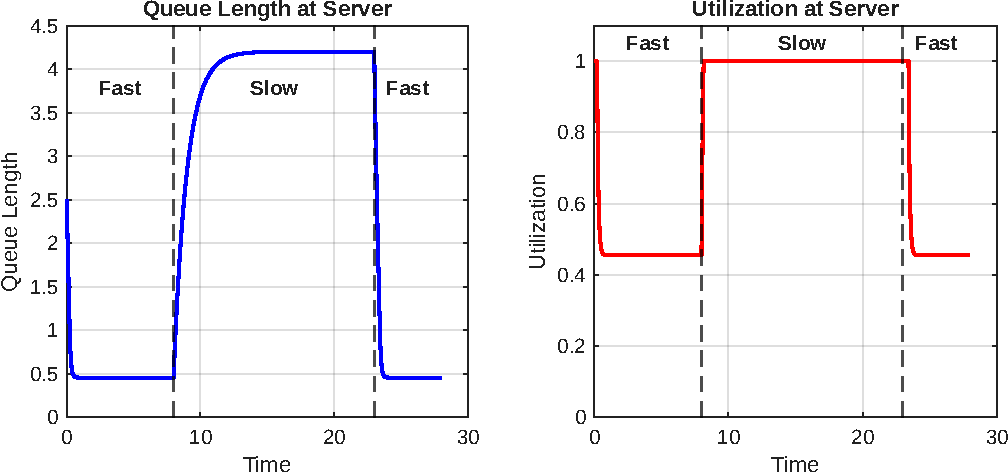
\includegraphics[width=0.6\textwidth]{images/envSamplePath}
\caption{Transient queue length and utilization evolution along a sample path.}
\label{fig:sample_path}
\end{figure}

\section{Examples}
\subsection{Example 1: Fast and slow service}
\label{example-1-random-environments}

This example demonstrates how to model a queueing system operating in a random environment, where system parameters (e.g., service rates) change according to an underlying environmental process.

The scenario models a server that alternates between ``Fast'' and ``Slow'' modes. In Fast mode, the service rate is 10.0 (low utilization). In Slow mode, the service rate is 0.8 (high utilization, near saturation). The environment switches from Fast$\to$Slow at rate 0.5 (mean time in Fast mode = 2.0) and from Slow$\to$Fast at rate 1.0 (mean time in Slow mode = 1.0).

We start by creating a base closed queueing network with a delay and a queue:
\begin{MATLAB}
\begin{lstlisting}[language = matlab]
baseModel = Network('BaseModel');
delay = Delay(baseModel, 'ThinkTime');
queue = Queue(baseModel, 'Fast/Slow Server', SchedStrategy.FCFS);

% Closed class with 5 jobs
N = 5;
jobclass = ClosedClass(baseModel, 'Jobs', N, delay);
delay.setService(jobclass, Exp(1.0));  % Think time = 1.0
queue.setService(jobclass, Exp(2.0));  % Placeholder

% Connect nodes in a cycle
baseModel.link(Network.serialRouting(delay, queue));
\end{lstlisting}
\end{MATLAB}
\begin{JAVA}
\begin{lstlisting}[language = java, basicstyle=\ttfamily\scriptsize]
Network baseModel = new Network("BaseModel");
Delay delay = new Delay(baseModel, "ThinkTime");
Queue queue = new Queue(baseModel, "Fast/Slow Server", SchedStrategy.FCFS);

// Closed class with 5 jobs
int N = 5;
ClosedClass jobclass = new ClosedClass(baseModel, "Jobs", N, delay, 0);
delay.setService(jobclass, new Exp(1.0));  // Think time = 1.0
queue.setService(jobclass, new Exp(2.0));  // Placeholder

// Connect nodes in a cycle
baseModel.link(Network.serialRouting(delay, queue));
\end{lstlisting}
\end{JAVA}
\begin{KOTLIN}
\begin{lstlisting}[language = kotlin, basicstyle=\ttfamily\scriptsize]
val baseModel = Network("BaseModel")
val delay = Delay(baseModel, "ThinkTime")
val queue = Queue(baseModel, "Fast/Slow Server", SchedStrategy.FCFS)

// Closed class with 5 jobs
val N = 5
val jobclass = ClosedClass(baseModel, "Jobs", N, delay, 0)
delay.setService(jobclass, Exp(1.0))  // Think time = 1.0
queue.setService(jobclass, Exp(2.0))  // Placeholder

// Connect nodes in a cycle
baseModel.link(Network.serialRouting(delay, queue))
\end{lstlisting}
\end{KOTLIN}
\begin{PYTHON}
\begin{lstlisting}[language = python]
base_model = Network('BaseModel')
delay = Delay(base_model, 'ThinkTime')
queue = Queue(base_model, 'Fast/Slow Server', SchedStrategy.FCFS)

# Closed class with 5 jobs
N = 5
jobclass = ClosedClass(base_model, 'Jobs', N, delay)
delay.setService(jobclass, Exp(1.0))  # Think time = 1.0
queue.setService(jobclass, Exp(2.0))  # Placeholder

# Connect nodes in a cycle
base_model.link(Network.serialRouting(delay, queue))
\end{lstlisting}
\end{PYTHON}

Next, we create the random environment with two stages, each having a different service rate:
\begin{MATLAB}
\begin{lstlisting}[language = matlab]
env = Environment('ServerModes');

% Stage 1: Fast mode (service rate = 10.0, low utilization)
fastModel = baseModel.copy();
fastQueue = fastModel.getNodeByName('Fast/Slow Server');
fastQueue.setService(fastModel.classes{1}, Exp(10.0));
env.addStage('Fast', 'operational', fastModel);

% Stage 2: Slow mode (service rate = 0.8, high utilization)
slowModel = baseModel.copy();
slowQueue = slowModel.getNodeByName('Fast/Slow Server');
slowQueue.setService(slowModel.classes{1}, Exp(0.8));
env.addStage('Slow', 'degraded', slowModel);

% Define transitions between stages
env.addTransition('Fast', 'Slow', Exp(0.5));  % Fast->Slow
env.addTransition('Slow', 'Fast', Exp(1.0));  % Slow->Fast
\end{lstlisting}
\end{MATLAB}
\begin{JAVA}
\begin{lstlisting}[language = java, basicstyle=\ttfamily\scriptsize]
int E = 2;
Environment env = new Environment("ServerModes", E);

// Stage 0: Fast mode (service rate = 10.0, low utilization)
Network fastModel = baseModel.copy();
Queue fastQueue = (Queue) fastModel.getNodeByName("Fast/Slow Server");
fastQueue.setService(fastModel.getClasses().get(0), new Exp(10.0));
env.addStage(0, "Fast", "operational", fastModel);

// Stage 1: Slow mode (service rate = 0.8, high utilization)
Network slowModel = baseModel.copy();
Queue slowQueue = (Queue) slowModel.getNodeByName("Fast/Slow Server");
slowQueue.setService(slowModel.getClasses().get(0), new Exp(0.8));
env.addStage(1, "Slow", "degraded", slowModel);

// Define transitions between stages
env.addTransition(0, 1, new Exp(0.5));  // Fast->Slow
env.addTransition(1, 0, new Exp(1.0));  // Slow->Fast
\end{lstlisting}
\end{JAVA}
\begin{KOTLIN}
\begin{lstlisting}[language = kotlin, basicstyle=\ttfamily\scriptsize]
val E = 2
val env = Environment("ServerModes", E)

// Stage 0: Fast mode (service rate = 10.0, low utilization)
val fastModel = baseModel.copy()
val fastQueue = fastModel.getNodeByName("Fast/Slow Server") as Queue
fastQueue.setService(fastModel.classes[0], Exp(10.0))
env.addStage(0, "Fast", "operational", fastModel)

// Stage 1: Slow mode (service rate = 0.8, high utilization)
val slowModel = baseModel.copy()
val slowQueue = slowModel.getNodeByName("Fast/Slow Server") as Queue
slowQueue.setService(slowModel.classes[0], Exp(0.8))
env.addStage(1, "Slow", "degraded", slowModel)

// Define transitions between stages
env.addTransition(0, 1, Exp(0.5))  // Fast->Slow
env.addTransition(1, 0, Exp(1.0))  // Slow->Fast
\end{lstlisting}
\end{KOTLIN}
\begin{PYTHON}
\begin{lstlisting}[language = python]
env = Environment('ServerModes', 2)

# Stage 0: Fast mode (service rate = 10.0, low utilization)
fast_model = base_model.copy()
fast_queue = fast_model.getNodeByName('Fast/Slow Server')
fast_queue.setService(fast_model.classes[0], Exp(10.0))
env.addStage(0, 'Fast', 'operational', fast_model)

# Stage 1: Slow mode (service rate = 0.8, high utilization)
slow_model = base_model.copy()
slow_queue = slow_model.getNodeByName('Fast/Slow Server')
slow_queue.setService(slow_model.classes[0], Exp(0.8))
env.addStage(1, 'Slow', 'degraded', slow_model)

# Define transitions between stages
env.addTransition(0, 1, Exp(0.5))  # Fast->Slow
env.addTransition(1, 0, Exp(1.0))  # Slow->Fast
\end{lstlisting}
\end{PYTHON}

Finally, we solve the model using \texttt{SolverENV} with the Fluid solver (\texttt{FLD}) as the sub-solver for each stage:
\begin{MATLAB}
\begin{lstlisting}[language = matlab]
% Initialize the environment
env.init();
stageTable = env.getStageTable()

% Solve using SolverENV with Fluid sub-solver
fldOptions = FLD.defaultOptions;
fldOptions.timespan = [0, 100];
solverFactory = @(m) FLD(m, fldOptions);

envSolver = ENV(env, solverFactory);
[QN, UN, TN] = envSolver.getAvg();

% Display environment-averaged results
envAvgTable = envSolver.getAvgTable()
\end{lstlisting}
The output shows the environment stages and performance metrics:
\begin{lstlisting}[language = matlab, basicstyle=\ttfamily\scriptsize]
stageTable =
  2x6 table
    Stage    Name       Type         Prob        HoldT           Model
    _____    ____    ___________    _______    __________    _____________
      1      Fast    operational    0.66667    {1x4 cell}    {1x1 Network}
      2      Slow    degraded       0.33333    {1x4 cell}    {1x1 Network}

envAvgTable =
  2x6 table
     Station     JobClass     QLen      Util      RespT      Tput
    _________    ________    ______    ______    _______    ______
    ThinkTime      Jobs      2.9961    2.9961          1    2.9961
    Server         Jobs      2.0039         1    0.66796         3
\end{lstlisting}
\end{MATLAB}
\begin{JAVA}
\begin{lstlisting}[language = java, basicstyle=\ttfamily\scriptsize]
// Solve using SolverENV with Fluid sub-solver
SolverOptions envOptions = new SolverOptions(SolverType.ENV);
envOptions.iter_tol = 0.01;

SolverOptions fldOptions = new SolverOptions(SolverType.FLD);
fldOptions.timespan[1] = 100;

NetworkSolver[] solvers = new NetworkSolver[E];
for (int e = 0; e < E; e++) {
    solvers[e] = new FLD(env.getModel(e));
    solvers[e].options = fldOptions;
}

ENV envSolver = new ENV(env, solvers, envOptions);
envSolver.getAvgTable().print();
\end{lstlisting}
\end{JAVA}
\begin{KOTLIN}
\begin{lstlisting}[language = kotlin, basicstyle=\ttfamily\scriptsize]
// Solve using SolverENV with Fluid sub-solver
val envOptions = SolverOptions(SolverType.ENV)
envOptions.iter_tol = 0.01

val fldOptions = SolverOptions(SolverType.FLD)
fldOptions.timespan[1] = 100.0

val solvers = Array(E) { e ->
    FLD(env.getModel(e)).apply { options = fldOptions }
}

val envSolver = ENV(env, solvers, envOptions)
envSolver.avgTable.print()
\end{lstlisting}
\end{KOTLIN}
\begin{PYTHON}
\begin{lstlisting}[language = python]
# Initialize and inspect the environment
env_table = env.getStageTable()
print(env_table)

# Solve using SolverENV with Fluid sub-solver
env_solver = ENV(env, lambda m: FLD(m))
Q, U, T = env_solver.getAvg()

# Display environment-averaged results
env_avg_table = env_solver.getAvgTable()
print(env_avg_table)
\end{lstlisting}
\end{PYTHON}

The results show that the server spends approximately 66.67\% of time in Fast mode and 33.33\% in Slow mode. The environment-averaged queue length at the server is approximately 2.0 jobs, which is a weighted combination of the queue lengths in the Fast and Slow stages.

\subsubsection{Analyzing sample paths with getSamplePathTable}
\label{sec:getSamplePathTable}

In addition to computing steady-state metrics averaged over the environment distribution, \texttt{SolverENV} provides a method to analyze specific sample paths through the environment states. This is useful when you want to understand the transient behavior of the system as it transitions through a known sequence of environment states.

The \texttt{getSamplePathTable} method accepts a specification of a sample path---a list of (stage, duration) pairs---and computes the transient performance metrics for each segment. For each segment, the method:
\begin{enumerate}
\item Initializes the model from the previous segment's final queue lengths (or uniform distribution for the first segment)
\item Runs transient analysis for the specified duration using the Fluid solver
\item Extracts the initial and final values of queue length, utilization, and throughput
\end{enumerate}

The output is a table with columns for segment index, stage name, duration, station, job class, and the initial/final values of each metric. An example of the transient behavior along a sample path is shown in Figure~\ref{fig:sample_path}, which depicts a sample path transitioning through environment states Fast $\rightarrow$ Slow $\rightarrow$ Fast. In the Fast stage (service rate = 10.0), the server operates at low utilization ($\approx$45\%), while in the Slow stage (service rate = 0.8), the server becomes saturated ($\approx$100\% utilization), causing queue buildup as arrivals accumulate faster than they can be processed.

\begin{MATLAB}
\begin{lstlisting}[language = matlab]
% Define a sample path: Fast for 8 time units, Slow for 15, Fast for 5
samplePath = {'Fast', 8.0; 'Slow', 15.0; 'Fast', 5.0};

% Compute transient metrics along the sample path
[T, segmentResults] = solver.getSamplePathTable(samplePath);

% Display the results table
disp(T);

% Access detailed transient trajectories for plotting
seg1_QLen = segmentResults{1}.QNt{2,1}.metric;  % Server queue length in segment 1
seg1_time = segmentResults{1}.QNt{2,1}.t;
\end{lstlisting}
\end{MATLAB}

\begin{JAVA}
\begin{lstlisting}[language = java, basicstyle=\ttfamily\scriptsize]
// Define a sample path: Stage1 for 8.0, Stage2 for 15.0, Stage1 for 5.0
List<Object[]> samplePath = new ArrayList<>();
samplePath.add(new Object[]{"Stage1", 8.0});
samplePath.add(new Object[]{"Stage2", 15.0});
samplePath.add(new Object[]{"Stage1", 5.0});

// Compute transient metrics along the sample path
SolverENV.SamplePathResult result = solver.getSamplePathTable(samplePath);

// Access segment results
for (SolverENV.SamplePathResult.SamplePathSegment seg : result.segments) {
    System.out.printf("Segment %d (%s): duration=%.1f, finalQ=%.3f%n",
        seg.segmentIndex, seg.stageName, seg.duration,
        seg.finalQ.get(0, 0));
}
\end{lstlisting}
\end{JAVA}

\begin{PYTHON}
\begin{lstlisting}[language = python]
# Define a sample path: Fast for 8.0, Slow for 15.0, Fast for 5.0
sample_path = [('Fast', 8.0), ('Slow', 15.0), ('Fast', 5.0)]

# Compute transient metrics along the sample path
df = solver.getSamplePathTable(sample_path)

# Display the results DataFrame
print(df)
\end{lstlisting}
\end{PYTHON}

The sample path can be specified using either stage names (strings) or stage indices (integers). Stages are 1-indexed in MATLAB and 0-indexed in Java/Python. The duration for each segment must be positive.

\subsection{Example 2: Breakdown and repair}
\label{example-2-breakdown-repair}
\textsc{Line} provides convenience methods to simplify the common case of modeling node failures and repairs in random environments. These methods automatically create UP and DOWN stages for nodes that can break down, configure service rates appropriately, and set up breakdown and repair transitions.

The primary method is \texttt{addNodeFailureRepair}, which creates both breakdown and repair transitions in a single call:
\begin{MATLAB}
\begin{lstlisting}[language = matlab]
env = Environment('ServerEnv');
env.addNodeFailureRepair(baseModel, 'Server1', Exp(0.1), Exp(1.0), Exp(0.5));
env.init();
\end{lstlisting}
\end{MATLAB}
\begin{JAVA}
\begin{lstlisting}[language = java, basicstyle=\ttfamily\scriptsize]
Environment env = new Environment("ServerEnv", 2);
env.addNodeFailureRepair(baseModel, "Server1",
    new Exp(0.1), new Exp(1.0), new Exp(0.5));
env.init();
\end{lstlisting}
\end{JAVA}
\begin{KOTLIN}
\begin{lstlisting}[language = kotlin, basicstyle=\ttfamily\scriptsize]
val env = Environment("ServerEnv", 2)
env.addNodeFailureRepair(baseModel, "Server1",
    Exp(0.1), Exp(1.0), Exp(0.5))
env.init()
\end{lstlisting}
\end{KOTLIN}
\begin{PYTHON}
\begin{lstlisting}[language=python]
env = Environment('ServerEnv', 2)
env.add_node_failure_repair(base_model, 'Server1',
    Exp(0.1), Exp(1.0), Exp(0.5))
env.init()
\end{lstlisting}
\end{PYTHON}
where \texttt{baseModel} is the network with normal (UP) service rates, \texttt{'Server1'} is the node name, \texttt{Exp(0.1)} is the breakdown distribution (mean time to failure = 10 time units), \texttt{Exp(1.0)} is the repair distribution (mean time to repair = 1 time unit), and \texttt{Exp(0.5)} is the service distribution when the node is down.

This method automatically:
\begin{itemize}
\item Creates an UP stage with the service rates of the base model
\item Creates a DOWN stage with the specified reduced service rate for the failed node
\item Adds a breakdown transition (UP $\rightarrow$ DOWN) with the given breakdown distribution
\item Adds a repair transition (DOWN $\rightarrow$ UP) with the given repair distribution
\end{itemize}

Alternative methods for more control include \texttt{addNodeBreakdown} and \texttt{addNodeRepair}, which can be called separately. Custom reset policies can be specified as optional parameters:
\begin{MATLAB}
\begin{lstlisting}[language = matlab]
resetBreakdown = @(q) 0*q;  % Clear queues on breakdown
resetRepair = @(q) q;       % Keep jobs on repair
env.addNodeFailureRepair(baseModel, 'Server1', Exp(0.1), Exp(1.0), ...
    Exp(0.5), resetBreakdown, resetRepair);
\end{lstlisting}
\end{MATLAB}
\begin{JAVA}
\begin{lstlisting}[language = java, basicstyle=\ttfamily\scriptsize]
Env.ResetQueueLengthsFunction resetBreakdown = input -> {
    Matrix result = new Matrix(input.getNumRows(), input.getNumCols());
    result.zero();  // Clear queues on breakdown
    return result;
};
env.addNodeFailureRepair(baseModel, "Server1", new Exp(0.1),
    new Exp(1.0), new Exp(0.5), resetBreakdown, input -> input);
\end{lstlisting}
\end{JAVA}
\begin{KOTLIN}
\begin{lstlisting}[language = kotlin, basicstyle=\ttfamily\scriptsize]
val resetBreakdown = Env.ResetQueueLengthsFunction { input ->
    Matrix(input.numRows, input.numCols).apply { zero() }
}
env.addNodeFailureRepair(baseModel, "Server1", Exp(0.1),
    Exp(1.0), Exp(0.5), resetBreakdown) { it }
\end{lstlisting}
\end{KOTLIN}
\begin{PYTHON}
\begin{lstlisting}[language=python]
reset_breakdown = lambda q: q * 0  # Clear queues on breakdown
reset_repair = lambda q: q         # Keep jobs on repair
env.add_node_failure_repair(base_model, 'Server1', Exp(0.1),
    Exp(1.0), Exp(0.5), reset_breakdown, reset_repair)
\end{lstlisting}
\end{PYTHON}

Reset policies can also be modified after environment creation using \texttt{setBreakdownResetPolicy} and \texttt{setRepairResetPolicy} methods.

\subsubsection{Retrieving reliability metrics}
\label{retrieving-reliability-metrics}
After solving an environment model with node breakdown and repair, reliability metrics can be retrieved using the \Matlab{\texttt{getReliabilityTable}}\Java{\texttt{getReliabilityTable}}\Kotlin{\texttt{getReliabilityTable}}\Python{\texttt{get\_reliability\_table}} method (aliases: \texttt{relT}, \texttt{getRelT}, \texttt{relTable}, \texttt{getRelTable}):
\begin{MATLAB}
\begin{lstlisting}[language = matlab, basicstyle=\ttfamily\scriptsize]
>> env.getReliabilityTable
ans =
  4x4 table
      Metric           Value           Unit                  Description
    __________    ______________    ___________    ________________________________
    MTTF          10               time units     Mean time to failure (UP -> DOWN)
    MTTR          1                time units     Mean time to repair (DOWN -> UP)
    MTBF          11               time units     Mean time between failures (MTTF + MTTR)
    Availability  0.90909          probability    Steady-state probability of UP state
\end{lstlisting}
\end{MATLAB}
\begin{JAVA}
\begin{lstlisting}[language = java, basicstyle=\ttfamily\scriptsize]
Map<String, Double> metrics = env.getReliabilityTable();
System.out.println("MTTF: " + metrics.get("MTTF"));
System.out.println("MTTR: " + metrics.get("MTTR"));
System.out.println("MTBF: " + metrics.get("MTBF"));
System.out.println("Availability: " + metrics.get("Availability"));
\end{lstlisting}
\end{JAVA}
\begin{KOTLIN}
\begin{lstlisting}[language = kotlin, basicstyle=\ttfamily\scriptsize]
val metrics = env.getReliabilityTable()
println("MTTF: ${metrics["MTTF"]}")
println("MTTR: ${metrics["MTTR"]}")
println("MTBF: ${metrics["MTBF"]}")
println("Availability: ${metrics["Availability"]}")
\end{lstlisting}
\end{KOTLIN}
\begin{PYTHON}
\begin{lstlisting}[language=python]
metrics = env.get_reliability_table()
print(f"MTTF: {metrics['MTTF']}")
print(f"MTTR: {metrics['MTTR']}")
print(f"MTBF: {metrics['MTBF']}")
print(f"Availability: {metrics['Availability']}")
\end{lstlisting}
\end{PYTHON}

The reliability metrics returned are:
\begin{itemize}
\item \textit{MTTF} (Mean Time To Failure): Expected time until breakdown from the UP state. For multiple failure modes, this uses the combined failure rate: $\lambda_{\text{total}} = \sum_i \lambda_i$.
\item \textit{MTTR} (Mean Time To Repair): Expected time to restore from the DOWN state. For multiple DOWN states, this is a weighted average based on steady-state probabilities.
\item \textit{MTBF} (Mean Time Between Failures): Sum of MTTF and MTTR.
\item \textit{Availability}: Steady-state probability of the system being in the UP state.
\end{itemize}

\subsection{Example 3: Markov-modulated service}
\label{example-3-MAPQN2RENV}

This example shows how to convert a queueing network with MMPP2 (Markov-Modulated Poisson Process) service into an equivalent random environment model using the \texttt{MAPQN2RENV} utility. MMPP2 is a 2-phase service process where the service rate switches between two values according to an underlying Markov chain. The \texttt{MAPQN2RENV} function automatically transforms such a model into a random environment with two stages, each having exponential service at the corresponding MMPP rate.

We create a closed queueing network with an MMPP2 service process:
\begin{MATLAB}
\begin{lstlisting}[language = matlab]
model = Network('ClosedQN');
queue1 = Queue(model, 'Queue1', SchedStrategy.FCFS);
queue2 = Queue(model, 'Queue2', SchedStrategy.FCFS);

% Closed class with 3 jobs
N = 3;
jobClass = ClosedClass(model, 'Class1', N, queue1);

% MMPP2 service: slow_rate=2.0, fast_rate=5.0, slow_to_fast=0.5, fast_to_slow=0.3
queue1.setService(jobClass, MMPP2(2.0, 5.0, 0.5, 0.3));
queue2.setService(jobClass, Exp(3.0));

model.link(Network.serialRouting(queue1, queue2));

% Convert to random environment
env = MAPQN2RENV(model);
env.printStageTable();
\end{lstlisting}
\end{MATLAB}
\begin{JAVA}
\begin{lstlisting}[language = java, basicstyle=\ttfamily\scriptsize]
Network model = new Network("ClosedQN");
Queue queue1 = new Queue(model, "Queue1", SchedStrategy.FCFS);
Queue queue2 = new Queue(model, "Queue2", SchedStrategy.FCFS);

// Closed class with 3 jobs
int N = 3;
ClosedClass jobClass = new ClosedClass(model, "Class1", N, queue1, 0);

// MMPP2 service: slow_rate=2.0, fast_rate=5.0, slow_to_fast=0.5, fast_to_slow=0.3
queue1.setService(jobClass, new MMPP2(2.0, 5.0, 0.5, 0.3));
queue2.setService(jobClass, new Exp(3.0));

model.link(Network.serialRouting(queue1, queue2));

// Convert to random environment
Environment env = MAPQN2RENV.MAPQN2RENV(model);
env.init();
env.printStageTable();
\end{lstlisting}
The output shows the resulting environment structure:
\begin{lstlisting}[language = java, basicstyle=\ttfamily\scriptsize]
Stage Table:
============
Stage 1: Phase0 (Type: item)
  - Network: ClosedQN_Phase0
  - Nodes: 2
  - Classes: 1
Stage 2: Phase1 (Type: item)
  - Network: ClosedQN_Phase1
  - Nodes: 2
  - Classes: 1

Transitions:
  Phase0 -> Phase1: rate = 0.5000
  Phase1 -> Phase0: rate = 0.3000
\end{lstlisting}
\end{JAVA}
\begin{KOTLIN}
\begin{lstlisting}[language = kotlin, basicstyle=\ttfamily\scriptsize]
val model = Network("ClosedQN")
val queue1 = Queue(model, "Queue1", SchedStrategy.FCFS)
val queue2 = Queue(model, "Queue2", SchedStrategy.FCFS)

// Closed class with 3 jobs
val N = 3
val jobClass = ClosedClass(model, "Class1", N, queue1, 0)

// MMPP2 service: slow_rate=2.0, fast_rate=5.0, slow_to_fast=0.5, fast_to_slow=0.3
queue1.setService(jobClass, MMPP2(2.0, 5.0, 0.5, 0.3))
queue2.setService(jobClass, Exp(3.0))

model.link(Network.serialRouting(queue1, queue2))

// Convert to random environment
val env = MAPQN2RENV.MAPQN2RENV(model)
env.init()
env.printStageTable()
\end{lstlisting}
\end{KOTLIN}
\begin{PYTHON}
\begin{lstlisting}[language = python]
from line_solver import Network, Queue, ClosedClass, SchedStrategy, Exp
from line_solver.distributions_native.markovian import MMPP2
from line_solver.api.io.converters import mapqn2renv

model = Network('ClosedQN')
queue1 = Queue(model, 'Queue1', SchedStrategy.FCFS)
queue2 = Queue(model, 'Queue2', SchedStrategy.FCFS)

# Closed class with 3 jobs
N = 3
job_class = ClosedClass(model, 'Class1', N, queue1)

# MMPP2 service: slow_rate=2.0, fast_rate=5.0, slow_to_fast=0.5, fast_to_slow=0.3
queue1.set_service(job_class, MMPP2(2.0, 5.0, 0.5, 0.3))
queue2.set_service(job_class, Exp(3.0))

model.link(model.serial_routing(queue1, queue2))

# Convert to random environment
env = mapqn2renv(model)
env.print_stage_table()
\end{lstlisting}
The output shows the resulting environment structure:
\begin{lstlisting}[language = python, basicstyle=\ttfamily\scriptsize]
Stage Table:
============
Stage 1: Phase0 (Type: item)
  - Network: ClosedQN_Phase0
  - Nodes: 2
  - Classes: 1
Stage 2: Phase1 (Type: item)
  - Network: ClosedQN_Phase1
  - Nodes: 2
  - Classes: 1
Transitions:
  Phase0 -> Phase1: rate = 0.5000
  Phase1 -> Phase0: rate = 0.3000
\end{lstlisting}
\end{PYTHON}

The resulting environment can then be analyzed using \texttt{SolverENV} as shown in Example 1.

\subsection{Example 4: semi-Markov process environments}
\label{example-4-SMP}

This example demonstrates the analysis of random environments with non-Markovian transition distributions using semi-Markov Processes. When environment transitions follow general distributions (e.g., Lognormal), the ENV solver should be run with the \texttt{'smp'} method.

Consider a system that alternates between two operational modes with log-normally distributed holding times in each stage. 

\begin{MATLAB}
\begin{lstlisting}[language = matlab]
% Create two network models for different modes
model1 = Network('Mode1');
source1 = Source(model1, 'Source');
queue1 = Queue(model1, 'Queue1', SchedStrategy.PS);
sink1 = Sink(model1, 'Sink');
jobClass1 = OpenClass(model1, 'Jobs');
source1.setArrival(jobClass1, Exp(1.0));
queue1.setService(jobClass1, Exp(2.0));
model1.link(Network.serialRouting(source1, queue1, sink1));

model2 = Network('Mode2');
source2 = Source(model2, 'Source');
queue2 = Queue(model2, 'Queue1', SchedStrategy.PS);
sink2 = Sink(model2, 'Sink');
jobClass2 = OpenClass(model2, 'Jobs');
source2.setArrival(jobClass2, Exp(1.0));
queue2.setService(jobClass2, Exp(0.8));
model2.link(Network.serialRouting(source2, queue2, sink2));

% Create environment with LogNormal transitions (non-Markovian)
envModel = Environment('SemiMarkovEnv');
envModel.addStage('Stage1', 'UP', model1);
envModel.addStage('Stage2', 'UP', model2);
envModel.addTransition('Stage1', 'Stage2', Lognormal(1.0, 0.5));  % Non-exponential
envModel.addTransition('Stage2', 'Stage1', Lognormal(0.5, 0.3));  % Non-exponential

% Enable SMP method for non-Markovian transitions
options = SolverOptions();
options.method = 'smp';
solver = SolverENV(envModel, @SolverFluid, options);
solver.runAnalyzer();
solver.result
\end{lstlisting}
\end{MATLAB}

\begin{JAVA}
\begin{lstlisting}[language = java, basicstyle=\ttfamily\scriptsize]
// Create two network models for different modes
Network model1 = new Network("Mode1");
Queue queue1 = new Queue(model1, "Queue1", SchedStrategy.PS);
OpenClass jobClass1 = new OpenClass(model1, "Jobs");
Source source1 = new Source(model1, "Source");
Sink sink1 = new Sink(model1, "Sink");
source1.setArrival(jobClass1, new Exp(1.0));
queue1.setService(jobClass1, new Exp(2.0));
model1.link(Network.serialRouting(source1, queue1, sink1));

Network model2 = new Network("Mode2");
Queue queue2 = new Queue(model2, "Queue1", SchedStrategy.PS);
OpenClass jobClass2 = new OpenClass(model2, "Jobs");
Source source2 = new Source(model2, "Source");
Sink sink2 = new Sink(model2, "Sink");
source2.setArrival(jobClass2, new Exp(1.0));
queue2.setService(jobClass2, new Exp(0.8));
model2.link(Network.serialRouting(source2, queue2, sink2));

// Create environment with LogNormal transitions (non-Markovian)
Environment envModel = new Environment("SemiMarkovEnv", 2);
envModel.addStage(0, "Stage1", "UP", model1);
envModel.addStage(1, "Stage2", "UP", model2);
envModel.addTransition(0, 1, new Lognormal(1.0, 0.5));  // Non-exponential
envModel.addTransition(1, 0, new Lognormal(0.5, 0.3));  // Non-exponential
envModel.init();

// Enable SMP method for non-Markovian transitions
SolverOptions options = new SolverOptions();
options.method = "smp";
SolverENV solver = new SolverENV(envModel,
    model -> new SolverFluid(model, options), options);
solver.runAnalyzer();
System.out.println(solver.result);
\end{lstlisting}
\end{JAVA}

\begin{KOTLIN}
\begin{lstlisting}[language = kotlin, basicstyle=\ttfamily\scriptsize]
// Create two network models for different modes
val model1 = Network("Mode1")
val queue1 = Queue(model1, "Queue1", SchedStrategy.PS)
val jobClass1 = OpenClass(model1, "Jobs")
val source1 = Source(model1, "Source")
val sink1 = Sink(model1, "Sink")
source1.setArrival(jobClass1, Exp(1.0))
queue1.setService(jobClass1, Exp(2.0))
model1.link(Network.serialRouting(source1, queue1, sink1))

val model2 = Network("Mode2")
val queue2 = Queue(model2, "Queue1", SchedStrategy.PS)
val jobClass2 = OpenClass(model2, "Jobs")
val source2 = Source(model2, "Source")
val sink2 = Sink(model2, "Sink")
source2.setArrival(jobClass2, Exp(1.0))
queue2.setService(jobClass2, Exp(0.8))
model2.link(Network.serialRouting(source2, queue2, sink2))

// Create environment with LogNormal transitions (non-Markovian)
val envModel = Environment("SemiMarkovEnv", 2)
envModel.addStage(0, "Stage1", "UP", model1)
envModel.addStage(1, "Stage2", "UP", model2)
envModel.addTransition(0, 1, Lognormal(1.0, 0.5))  // Non-exponential
envModel.addTransition(1, 0, Lognormal(0.5, 0.3))  // Non-exponential
envModel.init()

// Enable SMP method for non-Markovian transitions
val options = SolverOptions()
options.method = "smp"
val solver = SolverENV(envModel,
    { model -> SolverFluid(model, options) }, options)
solver.runAnalyzer()
println(solver.result)
\end{lstlisting}
\end{KOTLIN}

\begin{PYTHON}
\begin{lstlisting}[language = python]
from line_solver import Network, Queue, Source, Sink, OpenClass
from line_solver import SchedStrategy, Exp, Lognormal, Environment, ENV, FLD
from line_solver import SolverOptions

# Create two network models for different modes
model1 = Network('Mode1')
queue1 = Queue(model1, 'Queue1', SchedStrategy.PS)
job_class1 = OpenClass(model1, 'Jobs')
source1 = Source(model1, 'Source')
sink1 = Sink(model1, 'Sink')
source1.set_arrival(job_class1, Exp(1.0))
queue1.set_service(job_class1, Exp(2.0))
model1.link(model1.serial_routing(source1, queue1, sink1))

model2 = Network('Mode2')
queue2 = Queue(model2, 'Queue1', SchedStrategy.PS)
job_class2 = OpenClass(model2, 'Jobs')
source2 = Source(model2, 'Source')
sink2 = Sink(model2, 'Sink')
source2.set_arrival(job_class2, Exp(1.0))
queue2.set_service(job_class2, Exp(0.8))
model2.link(model2.serial_routing(source2, queue2, sink2))

# Create environment with LogNormal transitions (non-Markovian)
env_model = Environment('SemiMarkovEnv', 2)
env_model.add_stage(0, 'Stage1', 'UP', model1)
env_model.add_stage(1, 'Stage2', 'UP', model2)
env_model.add_transition(0, 1, Lognormal(1.0, 0.5))  # Non-exponential
env_model.add_transition(1, 0, Lognormal(0.5, 0.3))  # Non-exponential

# Enable SMP method for non-Markovian transitions
options = SolverOptions()
options.method = 'smp'
solver = ENV(env_model, lambda m: FLD(m), options=options)

# Run each solver
for s in solver._solvers:
    if s is not None:
        s.runAnalyzer()

# Get average results
QN, UN, TN = solver.avg()
print('Average Queue Lengths:', QN)
print('Average Utilizations:', UN)
print('Average Throughputs:', TN)
\end{lstlisting}
\end{PYTHON}

The \texttt{ENV} solver correctly handles this by using numerical integration to compute transition probabilities from the non-Markovian distribution functions, rather than assuming Markovian (memoryless) transitions.

\chapter{Parameter Inference}
\label{parameter-inference}

\textsc{Line} supports parameter inference, i.e., the estimation of queueing network model parameters from empirical data. Given observed system measurements such as response times, throughputs, queue lengths, and utilizations, the inference methods recover the model parameters---primarily service demands---that best explain the data. While the \textsc{Line} solvers perform {\em forward analysis} (computing performance metrics from model parameters), the inference functions address the {\em inverse problem}: recovering model parameters from observed metrics.

\begin{MATLAB}
\noindent The parameter inference methods additionally require the \emph{Optimization Toolbox}.
\end{MATLAB}
\begin{PYTHON}
\noindent The RNN estimator additionally requires PyTorch.
\end{PYTHON}

\noindent To cite the parameter inference methods, we recommend referencing~\cite{SpinnerCBK15,LiuHCA06,PerezCPS15,WangCS16,WangCKN16,GarbiIT20}.

%%%%%%%%%%%%%%%%%%%%%%%%%%%%%%%%%%%%%%%%%%%%%%%%%%%%%%%%%%%%%%%%
\section{Quick start}
\label{infer-quick-start}

The typical workflow for parameter estimation is:
\begin{enumerate}
\item Define a model: create a \textsc{Line} \texttt{Network} with known structure but unknown service demands (set to \texttt{NaN}).
\item Collect measurements: wrap observed data as \texttt{SampledMetric} objects, specifying the metric type, timestamps, values, node, and (optionally) job class.
\item Configure the estimator: create a \texttt{ParamEstimator} with the model and desired method.
\item Add data and estimate: add samples to the estimator, interpolate, and call \texttt{estimateAt} to obtain the estimated service demands.
\end{enumerate}

\noindent The following example estimates service demands at a PS queue in a closed network using the UBO method:

\begin{PYTHON}
\begin{lstlisting}[language=python]
import numpy as np
from line_solver import (Network, Delay, Queue, Exp,
    ClosedClass, SchedStrategy, MetricType)
from line_solver.inference import ParamEstimator, SampledMetric

# Step 1: Define the queueing network model
model = Network('model')
delay = Delay(model, 'Delay')
queue = Queue(model, 'Queue1', SchedStrategy.PS)
class1 = ClosedClass(model, 'Class1', 1, delay, 0)
class2 = ClosedClass(model, 'Class2', 2, delay, 0)

# Set known service times at the delay station
delay.setService(class1, Exp.fitMean(1.0))
delay.setService(class2, Exp.fitMean(1.0))

# Mark queue service demands as unknown (to be estimated)
queue.setService(class1, Exp(float('nan')))
queue.setService(class2, Exp(float('nan')))

# Define routing: each class cycles between delay and queue
P = model.initRoutingMatrix()
P.set(class1, class1, delay, queue, 1.0)
P.set(class1, class1, queue, delay, 1.0)
P.set(class2, class2, delay, queue, 1.0)
P.set(class2, class2, queue, delay, 1.0)
model.link(P)

# Step 2: Generate synthetic measurement data
# True demands are D1=0.1 and D2=0.3
n = 30
ts = np.arange(1, n + 1, dtype=float)
arvr1 = 2 * np.ones(n) - np.random.rand(n) * 0.15
arvr2 = np.ones(n) - np.random.rand(n) * 0.15
util = 0.1 * arvr1 + 0.3 * arvr2  # U = D1*lam1 + D2*lam2
respt1 = 0.1 / (1 - util)  # M/G/1 response time formula
respt2 = 0.3 / (1 - util)

# Step 3: Configure the estimator with the UBO method
options = ParamEstimator.defaultOptions()
options['method'] = 'ubo'
se = ParamEstimator(model, options)

# Step 4: Add observed samples and run estimation
se.addSamples(SampledMetric(MetricType.ArvR, ts, arvr1, queue, class1))
se.addSamples(SampledMetric(MetricType.ArvR, ts, arvr2, queue, class2))
se.addSamples(SampledMetric(MetricType.RespT, ts, respt1, queue, class1))
se.addSamples(SampledMetric(MetricType.RespT, ts, respt2, queue, class2))
se.addSamples(SampledMetric(MetricType.Util, ts, util, queue))
se.interpolate()  # align all samples to common timestamps
estVal = se.estimateAt(queue)
print('Estimated demands:', estVal)  # close to [0.1, 0.3]
\end{lstlisting}
\end{PYTHON}

\begin{MATLAB}
\begin{lstlisting}[language=matlab]
% Step 1: Define the queueing network model
model = Network('model');
node{1} = Delay(model, 'Delay');
node{2} = Queue(model, 'Queue1', SchedStrategy.PS);
jobclass{1} = ClosedClass(model, 'Class1', 1, node{1}, 0);
jobclass{2} = ClosedClass(model, 'Class2', 2, node{1}, 0);

% Set known service times at the delay station
node{1}.setService(jobclass{1}, Exp.fitMean(1.0));
node{1}.setService(jobclass{2}, Exp.fitMean(1.0));

% Mark queue service demands as unknown (to be estimated)
node{2}.setService(jobclass{1}, Exp(NaN));
node{2}.setService(jobclass{2}, Exp(NaN));

% Define routing: each class cycles between delay and queue
P = model.initRoutingMatrix();
P{jobclass{1},jobclass{1}}(node{1},node{2}) = 1;
P{jobclass{1},jobclass{1}}(node{2},node{1}) = 1;
P{jobclass{2},jobclass{2}}(node{1},node{2}) = 1;
P{jobclass{2},jobclass{2}}(node{2},node{1}) = 1;
model.link(P);

% Step 2: Generate synthetic measurement data
% True demands are D1=0.1 and D2=0.3
n = 30; ts = (1:n)';
arvr1 = 2*ones(n,1) - rand(n,1)*0.15;
arvr2 = ones(n,1) - rand(n,1)*0.15;
util = 0.1*arvr1 + 0.3*arvr2;   % U = D1*lam1 + D2*lam2
respt1 = 0.1 ./ (1 - util);     % M/G/1 response time formula
respt2 = 0.3 ./ (1 - util);

% Step 3: Configure the estimator with the UBO method
options = ParamEstimator.defaultOptions();
options.method = 'ubo';
se = ParamEstimator(model, options);

% Step 4: Add observed samples and run estimation
se.addSamples(SampledMetric(MetricType.ArvR, ts, arvr1, node{2}, jobclass{1}));
se.addSamples(SampledMetric(MetricType.ArvR, ts, arvr2, node{2}, jobclass{2}));
se.addSamples(SampledMetric(MetricType.RespT, ts, respt1, node{2}, jobclass{1}));
se.addSamples(SampledMetric(MetricType.RespT, ts, respt2, node{2}, jobclass{2}));
se.addSamples(SampledMetric(MetricType.Util, ts, util, node{2}));
se.interpolate();  % align all samples to common timestamps
estVal = se.estimateAt(node{2});
disp(estVal); % close to [0.1; 0.3]
\end{lstlisting}
\end{MATLAB}

\begin{JAVA}
\begin{lstlisting}[language=kotlin]
import jline.lang.Network;
import jline.lang.nodes.Delay;
import jline.lang.nodes.Queue;
import jline.lang.distributions.Exp;
import jline.lang.ClosedClass;
import jline.lang.constant.SchedStrategy;
import jline.lang.constant.MetricType;
import jline.inference.lang.ParamEstimator;
import jline.inference.lang.SampledMetric;

// Step 1: Define the queueing network model
Network model = new Network("model");
Delay delay = new Delay(model, "Delay");
Queue queue = new Queue(model, "Queue1", SchedStrategy.PS);
ClosedClass class1 = new ClosedClass(model, "Class1", 1, delay, 0);
ClosedClass class2 = new ClosedClass(model, "Class2", 2, delay, 0);
delay.setService(class1, Exp.fitMean(1.0));  // known
delay.setService(class2, Exp.fitMean(1.0));  // known
queue.setService(class1, new Exp(Double.NaN)); // unknown
queue.setService(class2, new Exp(Double.NaN)); // unknown
model.serialRouting(delay, queue);

// Step 2: Generate synthetic measurement data
// True demands are D1=0.1 and D2=0.3
int n = 30;
double[] ts = new double[n];
for (int i = 0; i < n; i++) ts[i] = i + 1;
Random rng = new Random();
double[] arvr1 = new double[n], arvr2 = new double[n];
double[] util = new double[n];
double[] respt1 = new double[n], respt2 = new double[n];
for (int i = 0; i < n; i++) {
    arvr1[i] = 2.0 - rng.nextDouble() * 0.15;
    arvr2[i] = 1.0 - rng.nextDouble() * 0.15;
    util[i] = 0.1 * arvr1[i] + 0.3 * arvr2[i];
    respt1[i] = 0.1 / (1 - util[i]);
    respt2[i] = 0.3 / (1 - util[i]);
}

// Step 3: Configure the estimator with the UBO method
EstimatorOptions options = ParamEstimator.defaultOptions();
options.method = "ubo";
ParamEstimator se = new ParamEstimator(model, options);

// Step 4: Add observed samples and run estimation
se.addSamples(new SampledMetric(MetricType.ArvR, ts, arvr1, queue, class1));
se.addSamples(new SampledMetric(MetricType.ArvR, ts, arvr2, queue, class2));
se.addSamples(new SampledMetric(MetricType.RespT, ts, respt1, queue, class1));
se.addSamples(new SampledMetric(MetricType.RespT, ts, respt2, queue, class2));
se.addSamples(new SampledMetric(MetricType.Util, ts, util, queue));
se.interpolate(); // align all samples to common timestamps
double[] estVal = se.estimateAt(Arrays.asList(queue));
// close to [0.1, 0.3]
\end{lstlisting}
\end{JAVA}

\begin{KOTLIN}
\begin{lstlisting}[language=kotlin]
import jline.lang.Network
import jline.lang.nodes.Delay
import jline.lang.nodes.Queue
import jline.lang.distributions.Exp
import jline.lang.ClosedClass
import jline.lang.constant.SchedStrategy
import jline.lang.constant.MetricType
import jline.inference.lang.ParamEstimator
import jline.inference.lang.SampledMetric

// Step 1: Define the queueing network model
val model = Network("model")
val delay = Delay(model, "Delay")
val queue = Queue(model, "Queue1", SchedStrategy.PS)
val class1 = ClosedClass(model, "Class1", 1, delay, 0)
val class2 = ClosedClass(model, "Class2", 2, delay, 0)
delay.setService(class1, Exp.fitMean(1.0))   // known
delay.setService(class2, Exp.fitMean(1.0))   // known
queue.setService(class1, Exp(Double.NaN))    // unknown
queue.setService(class2, Exp(Double.NaN))    // unknown
model.serialRouting(delay, queue)

// Step 2: Generate synthetic measurement data
// True demands are D1=0.1 and D2=0.3
val n = 30
val ts = DoubleArray(n) { (it + 1).toDouble() }
val rng = java.util.Random()
val arvr1 = DoubleArray(n) { 2.0 - rng.nextDouble() * 0.15 }
val arvr2 = DoubleArray(n) { 1.0 - rng.nextDouble() * 0.15 }
val util = DoubleArray(n) { 0.1 * arvr1[it] + 0.3 * arvr2[it] }
val respt1 = DoubleArray(n) { 0.1 / (1 - util[it]) }
val respt2 = DoubleArray(n) { 0.3 / (1 - util[it]) }

// Step 3: Configure the estimator with the UBO method
val options = ParamEstimator.defaultOptions()
options.method = "ubo"
val se = ParamEstimator(model, options)

// Step 4: Add observed samples and run estimation
se.addSamples(SampledMetric(MetricType.ArvR, ts, arvr1, queue, class1))
se.addSamples(SampledMetric(MetricType.ArvR, ts, arvr2, queue, class2))
se.addSamples(SampledMetric(MetricType.RespT, ts, respt1, queue, class1))
se.addSamples(SampledMetric(MetricType.RespT, ts, respt2, queue, class2))
se.addSamples(SampledMetric(MetricType.Util, ts, util, queue))
se.interpolate() // align all samples to common timestamps
val estVal = se.estimateAt(listOf(queue))
println("Estimated demands: ${estVal.contentToString()}")
// close to [0.1, 0.3]
\end{lstlisting}
\end{KOTLIN}

%%%%%%%%%%%%%%%%%%%%%%%%%%%%%%%%%%%%%%%%%%%%%%%%%%%%%%%%%%%%%%%%
\section{Specifying measurement data}
\label{infer-classes}

Parameter estimation requires observed performance measurements to be provided as \texttt{SampledMetric} objects. Each \texttt{SampledMetric} encapsulates a single time series and is constructed from the following arguments:
\begin{enumerate}
\item A metric type (one of \texttt{MetricType.ArvR}, \texttt{MetricType.RespT}, \texttt{MetricType.Util}, \texttt{MetricType.QLen}, or \texttt{MetricType.Tput}).
\item A vector of timestamps \texttt{ts}, of length~$n$.
\item A vector of observed values \texttt{data}, also of length~$n$, where \texttt{data[k]} is the measurement taken at time \texttt{ts[k]}.
\item The node at which the measurements were taken (e.g., a \texttt{Queue} or \texttt{Delay} station).
\item Optionally, the job class to which the measurements refer. If omitted, the metric is treated as an aggregate measurement across all classes.
\end{enumerate}

\noindent The five metric types are summarized below:
\begin{center}
\begin{tabular}{|l|l|l|}
\hline
\textbf{Metric type} & \textbf{Description} & \textbf{Unit / range} \\
\hline
\texttt{ArvR} & Arrival rate at the node & jobs / time unit \\
\texttt{RespT} & Response time (waiting + service) & time units \\
\texttt{Util} & Utilization of server capacity & $[0,1]$ \\
\texttt{QLen} & Queue length (jobs present at the node) & jobs (non-negative) \\
\texttt{Tput} & Throughput (completions at the node) & jobs / time unit \\
\hline
\end{tabular}
\end{center}

\noindent Timestamps and values must be numeric vectors of the same length. The timestamps should be monotonically increasing and represent the instants at which each measurement was collected. The values represent the observed metric at each timestamp. The following example creates a \texttt{SampledMetric} containing 30 per-class arrival rate observations at a queue:
\begin{PYTHON}
\begin{lstlisting}[language=python]
ts = np.arange(1, 31, dtype=float)          # 30 timestamps: [1, 2, ..., 30]
data = 2 * np.ones(30) + np.random.rand(30) # 30 observed arrival rates
sample = SampledMetric(MetricType.ArvR, ts, data, queue, class1)
\end{lstlisting}
\end{PYTHON}
\begin{MATLAB}
\begin{lstlisting}[language=matlab]
ts = (1:30)';                              % 30 timestamps: [1; 2; ...; 30]
data = 2*ones(30,1) + rand(30,1);          % 30 observed arrival rates
sample = SampledMetric(MetricType.ArvR, ts, data, node{2}, jobclass{1});
\end{lstlisting}
\end{MATLAB}

\noindent When the job class argument is omitted, the metric is treated as an aggregate measurement across all classes. This is common for utilization data, which monitoring tools typically report at the station level rather than per class:
\begin{PYTHON}
\begin{lstlisting}[language=python]
util_sample = SampledMetric(MetricType.Util, ts, util_data, queue)
\end{lstlisting}
\end{PYTHON}
\begin{MATLAB}
\begin{lstlisting}[language=matlab]
util_sample = SampledMetric(MetricType.Util, ts, util_data, node{2});
\end{lstlisting}
\end{MATLAB}

\noindent Different estimation methods require different combinations of metric types (see Table~\ref{TAB_infer_methods}). For example, UBR requires per-class arrival rates and station utilization, while MCMC requires per-class queue-length samples.

\subsection{Periodic samples and trace data}

By default, a \texttt{SampledMetric} represents periodic samples: the values are averages or snapshots collected at regular intervals. Some estimation methods (MLPS, FMLPS, Gibbs) instead require individual job traces, where each entry records a single job event. In a trace, timestamps are irregular (one per event rather than one per interval), and values represent instantaneous observations for that event. To indicate that a \texttt{SampledMetric} contains trace data, call \texttt{set\_trace()}:
\begin{PYTHON}
\begin{lstlisting}[language=python]
# arrival_times[k]: time of the k-th arrival
# rates[k]: instantaneous arrival rate at that time
arvr_trace = SampledMetric(MetricType.ArvR, arrival_times, rates, queue, class1)
arvr_trace.set_trace()
\end{lstlisting}
\end{PYTHON}
\begin{MATLAB}
\begin{lstlisting}[language=matlab]
% arrival_times(k): time of the k-th arrival
% rates(k): instantaneous arrival rate at that time
arvr_trace = SampledMetric(MetricType.ArvR, arrival_times, rates, node{2}, jobclass{1});
arvr_trace.setTrace();
\end{lstlisting}
\end{MATLAB}

\subsection{Conditional metrics}

Some estimation methods require measurements that were recorded conditionally upon a specific event. For example, the ERPS estimator uses queue-length observations collected only at the instants when a job of a given class arrives. This conditional relationship is expressed using the \texttt{Event} class:
\begin{PYTHON}
\begin{lstlisting}[language=python]
from line_solver.inference import Event
evt = Event(EventType.ARV, queue, class1)   # arrivals of class1
ql = SampledMetric(MetricType.QLen, ts, ql_data, queue)
ql.set_conditional(evt)                     # queue length seen by arriving class1 jobs
\end{lstlisting}
\end{PYTHON}
\begin{MATLAB}
\begin{lstlisting}[language=matlab]
evt = Event(EventType.ARV, node{2}, jobclass{1}); % arrivals of class1
ql = SampledMetric(MetricType.QLen, ts, ql_data, node{2});
ql.setConditional(evt);                            % queue length seen by arriving class1 jobs
\end{lstlisting}
\end{MATLAB}

\subsection{Configuring and running the estimator}
\label{sec:infer-param-estimator}

The \texttt{ParamEstimator} takes a \textsc{Line} \texttt{Network} model in which the unknown service demands are set to \texttt{Exp(NaN)}. After adding all measurement samples, a call to \texttt{interpolate()} aligns the time series onto common timestamps (using linear interpolation so that all metrics share the same time grid), and \texttt{estimateAt()} runs the estimation:
\begin{PYTHON}
\begin{lstlisting}[language=python]
options = ParamEstimator.defaultOptions()
options['method'] = 'ubo'                  # choose estimation method
se = ParamEstimator(model, options)
se.addSamples(arvr_sample)                 # add each SampledMetric
se.addSamples(respt_sample)
se.addSamples(util_sample)
se.interpolate()                           # align timestamps
estVal = se.estimateAt(queue)              # returns estimated demands
\end{lstlisting}
\end{PYTHON}
\begin{MATLAB}
\begin{lstlisting}[language=matlab]
options = ParamEstimator.defaultOptions();
options.method = 'ubo';                    % choose estimation method
se = ParamEstimator(model, options);
se.addSamples(arvr_sample);               % add each SampledMetric
se.addSamples(respt_sample);
se.addSamples(util_sample);
se.interpolate();                          % align timestamps
estVal = se.estimateAt(node{2});           % returns estimated demands
\end{lstlisting}
\end{MATLAB}

\noindent The \texttt{estimateAt} method returns the estimated service demands and also updates the model's service distributions in-place. If the best method is not known in advance, \texttt{auto\_method()} selects one automatically based on the types of data that have been added.

\label{sec:infer-options}
The estimator accepts several configuration options through \texttt{ParamEstimator.defaultOptions()}. The \texttt{method} option selects the estimation algorithm (see Section~\ref{infer-estimation-methods}; default: \texttt{'ubr'}). The \texttt{solver} option specifies the forward solver used during estimation (default: \texttt{SolverMVA}). Iterative methods respect \texttt{iter\_max} (default: 1000) and \texttt{tol} (default: $10^{-3}$). For open networks, several methods automatically construct a closed equivalent with population controlled by \texttt{openPopulation} (default: 100).

%%%%%%%%%%%%%%%%%%%%%%%%%%%%%%%%%%%%%%%%%%%%%%%%%%%%%%%%%%%%%%%%
\section{Estimation methods}
\label{infer-estimation-methods}

\textsc{Line} provides twelve estimation methods, each suited to different data availability scenarios. Table~\ref{TAB_infer_methods} summarizes all methods along with their required input data and references.

{\centering
\begin{longtable}{|p{1.2cm}|p{3.2cm}|p{0.42\linewidth}|p{2.8cm}|}
\caption{Estimation methods for \texttt{ParamEstimator}.}\label{TAB_infer_methods}\\
\hline
\textbf{Method}	&\textbf{Required Data}	& \textbf{Description} & \textbf{Refs.} \\
\hline
\endfirsthead
\multicolumn{4}{c}%
{\tablename\ \thetable\ -- Estimation methods.\textit{ Continued from previous page}} \\
\hline
\textbf{Method}	&\textbf{Required Data}	& \textbf{Description} & \textbf{Refs.} \\
\hline
	\endhead
\hline \multicolumn{4}{r}{\textit{Continued on next page}} \\
\endfoot
\hline
\endlastfoot
\hline
\texttt{ubr} & ArvR, Util & Utilization-based non-negative least squares regression & \cite{SpinnerCBK15}\\
\hline
\texttt{ubo} & ArvR, RespT, Util & Utilization-based constrained quadratic optimization & \cite{LiuHCA06}\\
\hline
\texttt{erps} & RespT (trace), QLen (cond.) & Extended regression for processor sharing stations & \cite{PerezCPS15}\\
\hline
\texttt{ekf} & ArvR, RespT, Util & Sequential estimation via Extended Kalman Filter & \cite{SpinnerCBK15}\\
\hline
\texttt{mle} & ArvR, RespT, Util & Maximum likelihood via bounded optimization with forward solver & \cite{PerezCPS15}\\
\hline
\texttt{mcmc} & QLen (aggregate) & Gibbs sampling with product-form queueing network likelihood & \cite{WangCS16}\\
\hline
\texttt{qmle} & QLen (per-class) & Closed-form quick maximum likelihood estimation & \cite{WangCKN16}\\
\hline
\texttt{mlps} & ArvR (trace), RespT (trace) & Exact CTMC-based maximum likelihood for PS stations & \cite{PerezCPS15}\\
\hline
\texttt{fmlps} & ArvR (trace), RespT (trace) & Fluid-limit maximum likelihood for PS stations & \cite{PerezCPS15}\\
\hline
\texttt{gibbs} & ArvR (trace), RespT (trace), Tput & Gibbs sampling from individual job trace data & \cite{WangCS16}\\
\hline
\texttt{rnn} & QLen (per-class, trace) & Physics-informed recurrent neural network & \cite{GarbiIT20}\\
\hline
\end{longtable}
} % centering


\section{Inference examples}
\label{infer-examples}

\Matlab{The table below lists the inference example scripts available under the \texttt{examples/inference/} folder.}
\Python{The table below lists the inference example scripts available under the \texttt{examples/inference/} folder.}
\Java{The inference examples are available as test classes in the \texttt{jline.inference} package under the \texttt{jar/src/test/kotlin/} folder.}
\Kotlin{The inference examples are available as test classes in the \texttt{jline.inference} package under the \texttt{jar/src/test/kotlin/} folder.}
\begin{footnotesize}
\begin{longtable}{|p{0.42\linewidth}|p{0.53\linewidth}|}
\caption{Inference examples}
\\\hline
\textbf{Example} & \textbf{Problem}
\\\hline
\endfirsthead
\multicolumn{2}{c}%
{\tablename\ \thetable\ -- Inference examples.\textit{ Continued from previous page}} \\
\hline
\textbf{Example} & \textbf{Problem}\\
\hline
\endhead
\hline \multicolumn{2}{r}{\textit{Continued on next page}} \\
\endfoot
\hline
\endlastfoot
\hline
\multicolumn{2}{|l|}{\textit{Utilization-Based Regression (UBR)}} \\
\hline
\texttt{est\_ubr\_closed} & UBR estimation in a closed queueing network\\
\texttt{est\_ubr\_open} & UBR estimation in an open queueing network\\
\texttt{est\_ubr\_changepoint} & UBR estimation with workload change-point detection\\
\hline
\multicolumn{2}{|l|}{\textit{Utilization-Based Optimization (UBO)}} \\
\hline
\texttt{est\_ubo\_closed} & UBO estimation in a closed queueing network\\
\texttt{est\_ubo\_open} & UBO estimation in an open queueing network\\
\texttt{est\_ubo\_changepoint} & UBO estimation with workload change-point detection\\
\texttt{est\_ubo\_variants\_closed} & Comparison of UBO and MLE estimators in a closed network\\
\hline
\multicolumn{2}{|l|}{\textit{Extended Kalman Filter (EKF)}} \\
\hline
\texttt{est\_ekf\_closed} & EKF estimation in a closed queueing network\\
\texttt{est\_ekf\_open} & EKF estimation in an open queueing network\\
\texttt{est\_ekf\_changepoint} & EKF estimation with workload change-point detection\\
\hline
\multicolumn{2}{|l|}{\textit{Maximum Likelihood (MLE)}} \\
\hline
\texttt{est\_mle\_open} & MLE estimation in an open queueing network\\
\hline
\multicolumn{2}{|l|}{\textit{Markov Chain Monte Carlo (MCMC)}} \\
\hline
\texttt{est\_mcmc\_closed} & MCMC estimation in a closed queueing network\\
\hline
\multicolumn{2}{|l|}{\textit{Quick Maximum Likelihood (QMLE)}} \\
\hline
\texttt{est\_qmle\_closed} & QMLE estimation in a closed queueing network\\
\hline
\multicolumn{2}{|l|}{\textit{Extended Regression for PS (ERPS)}} \\
\hline
\texttt{est\_erps\_closed} & ERPS estimation in a closed queueing network\\
\texttt{est\_erps\_open} & ERPS estimation in an open queueing network\\
\hline
\multicolumn{2}{|l|}{\textit{Recurrent Neural Network (RNN)}} \\
\hline
\texttt{est\_rnn\_closed} & RNN estimation from queue-length traces\\
\hline
\multicolumn{2}{|l|}{\textit{Trace-Based Estimation}} \\
\hline
\texttt{est\_trace\_closed} & Trace-based estimation (MLPS/FMLPS) in a closed network\\
\hline
\end{longtable}
\end{footnotesize}


\appendix

\chapter{Command-Line Interface (line-cli)}
\label{command-line-interface}

The \textsc{Line} command-line interface (\texttt{line-cli}) provides a standalone tool for solving queueing network models directly from the terminal. This interface is useful for batch processing, integration with external tools, scripting, and environments where interactive use of MATLAB, Python, or Java is not desirable.

\section{Installation}
\label{cli-installation}

The CLI tool requires:
\begin{itemize}
\item {Java 8+}: The Java Runtime Environment (JRE) version 8 or later.
\item {Python 3.11+}: Python 3.11 or later.
\item {jline.jar}: The \textsc{Line} solver JAR file, typically located in the \texttt{common/} directory.
\end{itemize}

The CLI is included in the standard \textsc{Line} distribution. After extracting the release archive, verify the installation by running:
\begin{lstlisting}[language=bash, basicstyle=\ttfamily\footnotesize]
python line-cli.py info
\end{lstlisting}

If the JAR file is not automatically detected, set the \texttt{LINE\_JAR\_PATH} environment variable:
\begin{lstlisting}[language=bash, basicstyle=\ttfamily\footnotesize]
export LINE_JAR_PATH=/path/to/jline.jar
\end{lstlisting}

\section{Basic Usage}
\label{cli-basic-usage}

The CLI supports several commands for solving models and querying information.

\subsection{Solving a Model}
To solve a queueing network model, use the \texttt{solve} command with the mandatory \texttt{-s} (or \texttt{--solver}) option to specify the solver algorithm:
\begin{lstlisting}[language=bash, basicstyle=\ttfamily\footnotesize]
python line-cli.py solve model.jsimg -s mva
\end{lstlisting}

If you are unsure of which solver to use, the \texttt{auto} solver provides an automatic choice. To list all available solvers:
\begin{lstlisting}[language=bash, basicstyle=\ttfamily\footnotesize]
python line-cli.py list solvers
\end{lstlisting}
The following table summarizes the solvers presently interfaced with the cli tool:
\begin{center}
\begin{tabular}{|l|l|l|l|}
\hline
\textbf{Solver} & \textbf{Name} & \textbf{Formats} & \textbf{Notes} \\
\hline
\texttt{auto} & Automatic Selection & All & Selects best solver for model \\
\texttt{ctmc} & CTMC & jsim/jsimg/jsimw & Exact, small models only \\
\texttt{ldes} & LDES (LINE Discrete Event Simulator) & jsim/jsimg/jsimw & Simulation-based \\
\texttt{fld} & Fluid ODE & jsim/jsimg/jsimw & Fast, approximate \\
\texttt{jmt} & Java Modelling Tools & jsim/jsimg/jsimw & External simulation \\
\texttt{ln} & Layered Network & lqnx/xml & For LQN models \\
\texttt{lqns} & LQN Solver & lqnx/xml & External LQNS tool \\
\texttt{mam} & Matrix Analytic & jsim/jsimg/jsimw & Supports Fork-Join percentiles \\
\texttt{mva} & Mean Value Analysis & jsim/jsimg/jsimw & Fast, general purpose \\
\texttt{nc} & Normalizing Constant & jsim/jsimg/jsimw & Exact analysis \\
\texttt{qns} & QNS & jsim/jsimg/jsimw & External QNSolver integration \\
\texttt{ssa} & Stochastic Simulation & jsim/jsimg/jsimw & State-space sampling \\
\hline
\end{tabular}
\end{center}

The input format is automatically detected from the file extension. Supported formats include:
\begin{itemize}
\item \texttt{.jsimg}, \texttt{.jsim}, \texttt{.jsimw}: JMT simulation model formats
\item \texttt{.lqnx}, \texttt{.xml}: Layered Queueing Network Solver XML format
\end{itemize}
Models can also be piped via stdin when the input format is specified:
\begin{lstlisting}[language=bash, basicstyle=\ttfamily\footnotesize]
cat model.jsimg | python line-cli.py solve -i jsimg -s mva
\end{lstlisting}

The CLI also supports multiple output formats via the \texttt{-o} or \texttt{--output-format} option:
\begin{lstlisting}[language=bash, basicstyle=\ttfamily\footnotesize]
python line-cli.py solve model.jsimg -s mva -o table   # Human-readable table
python line-cli.py solve model.jsimg -s mva -o json    # JSON format
python line-cli.py solve model.jsimg -s mva -o csv     # Comma-separated values
python line-cli.py solve model.jsimg -s mva -o raw     # Raw solver output
\end{lstlisting}
If unspecified, the table output format is used by default.

To save results to a file, further add the \texttt{-O} option:
\begin{lstlisting}[language=bash, basicstyle=\ttfamily\footnotesize]
python line-cli.py solve model.jsimg -s mva -o json -O results.json
\end{lstlisting}

\subsection{Analysis Types}
\label{cli-analysis-types}

The \texttt{-a} or \texttt{--analysis} option specifies which metrics to compute:
\begin{lstlisting}[language=bash, basicstyle=\ttfamily\footnotesize]
python line-cli.py solve model.jsimg -s mva -a all   # Average and system metrics (default)
python line-cli.py solve model.jsimg -s mva -a avg   # Average metrics only
python line-cli.py solve model.jsimg -s mva -a sys   # System metrics only
\end{lstlisting}

Advanced analysis types include:
\begin{itemize}
\item \texttt{stage}, \texttt{chain}, \texttt{node}, \texttt{nodechain}: stage-, chain-, node-, and node-chain-level averages
\item \texttt{cdf-respt}, \texttt{cdf-passt}: Response/passage time CDFs
\item \texttt{perct-respt}: Response time percentiles (MAM solver)
\item \texttt{tran-avg}, \texttt{tran-cdf-respt}, \texttt{tran-cdf-passt}: transient averages and transient CDFs
\item \texttt{prob}, \texttt{prob-aggr}, \texttt{prob-marg}: State probabilities (CTMC/SSA)
\item \texttt{prob-sys}, \texttt{prob-sys-aggr}: System state probabilities
\item \texttt{sample}, \texttt{sample-aggr}, \texttt{sample-sys}, \texttt{sample-sys-aggr}: State trajectory sampling (SSA)
\item \texttt{reward}, \texttt{reward-steady}, \texttt{reward-value}: Reward metrics (CTMC)
\end{itemize}

To list all analysis types:
\begin{lstlisting}[language=bash, basicstyle=\ttfamily\footnotesize]
python line-cli.py list analysis
\end{lstlisting}

\section{Server Modes}
\label{cli-server-modes}

The CLI can run as a server to accept solve requests over the network.

\subsection{WebSocket Server}
Start a WebSocket server for real-time communication:
\begin{lstlisting}[language=bash, basicstyle=\ttfamily\footnotesize]
python line-cli.py server -p 5863
\end{lstlisting}
This starts a WebSocket server on port 5863 (default). Clients can connect to \texttt{ws://localhost:5863} to submit models and receive results.

\subsection{REST API Server}
Start a REST API server for HTTP-based integration:
\begin{lstlisting}[language=bash, basicstyle=\ttfamily\footnotesize]
python line-cli.py rest -p 8080
\end{lstlisting}
Available endpoints:
\begin{itemize}
\item \texttt{POST /solve}: Submit a model for solving
\item \texttt{GET /health}: Health check endpoint
\end{itemize}

\section{Advanced Options}
\label{cli-advanced-options}

\subsection{Stochastic Solver Options}
For stochastic solvers (LDES, SSA, JMT), a random seed can be specified for reproducibility:
\begin{lstlisting}[language=bash, basicstyle=\ttfamily\footnotesize]
python line-cli.py solve model.jsimg -s ssa -d 12345
\end{lstlisting}

\subsection{Probability and Sampling Options}
For probability and sampling analysis:
\begin{lstlisting}[language=bash, basicstyle=\ttfamily\footnotesize]
# State probability at node 0
python line-cli.py solve model.jsimg -s ctmc -a prob -n 0

# Sample 5000 events from node 1
python line-cli.py solve model.jsimg -s ssa -a sample -n 1 --events 5000

# Compute specific percentiles
python line-cli.py solve model.jsimg -s mam -a perct-respt --percentiles 50,90,95,99
\end{lstlisting}

\subsection{Output Metrics}
\label{cli-output-metrics}

The CLI outputs performance metrics organized in two tables.

Average Metrics (per station and job class):
\begin{center}
\begin{tabular}{|l|l|}
\hline
\texttt{QLen} & Average queue length (number of jobs) \\
\texttt{Util} & Server utilization (0--1) \\
\texttt{RespT} & Response time (seconds) \\
\texttt{ResidT} & Residence time (seconds) \\
\texttt{Tput} & Throughput (jobs/second) \\
\texttt{ArvR} & Arrival rate (jobs/second) \\
\hline
\end{tabular}
\end{center}

System Metrics (per chain):
\begin{center}
\begin{tabular}{|l|l|}
\hline
\texttt{SysRespT} & End-to-end response time \\
\texttt{SysTput} & System throughput \\
\texttt{SysQLen} & Total jobs in system \\
\hline
\end{tabular}
\end{center}

\section{Command Reference}
\label{cli-command-reference}

\begin{center}
\begin{tabular}{|l|l|}
\hline
\textbf{Command/Option} & \textbf{Description} \\
\hline
\texttt{solve <file>} & Solve a queueing model \\
\texttt{info} & Display system information \\
\texttt{list solvers} & List available solvers \\
\texttt{list formats} & List supported formats \\
\texttt{list analysis} & List analysis types \\
\texttt{server} & Start WebSocket server \\
\texttt{rest} & Start REST API server \\
\hline
\texttt{-s, --solver} & Solver algorithm \\
\texttt{-i, --input-format} & Input format (auto-detected) \\
\texttt{-o, --output-format} & Output format (table/json/csv/raw) \\
\texttt{-a, --analysis} & Analysis type(s) \\
\texttt{-d, --seed} & Random seed \\
\texttt{-e, --maxevents} & Maximum simulation events (LDES) \\
\texttt{-n, --node} & Node index (for prob/sample) \\
\texttt{-c, --class-idx} & Class index (for prob-marg) \\
\texttt{-v, --verbose} & Verbose output \\
\texttt{-q, --quiet} & Suppress status messages \\
\texttt{-O, --output-file} & Write results to file \\
\texttt{-p, --port} & Server port \\
\texttt{-H, --host} & Server host address \\
\hline
\end{tabular}
\end{center}

\section{Examples}
\label{cli-examples}

\subsection{Sample Output}
Running the CLI on a sample open queueing network model:
\begin{lstlisting}[language=bash, basicstyle=\ttfamily\footnotesize]
python line-cli.py solve example.jsimg -s mva
\end{lstlisting}
produces the following output:
\begin{lstlisting}[basicstyle=\ttfamily\scriptsize]
Solving example.jsimg...

Average Metrics
===============
Station   Class    Metric  Value    Unit
----------------------------------------
Source 1  Class A  QLen    0
Source 1  Class A  Util    0
Source 1  Class A  RespT   0
Source 1  Class A  Tput    2
Source 1  Class B  QLen    0
Source 1  Class B  Tput    1
Queue 1   Class A  QLen    1.33318
Queue 1   Class A  Util    0.4
Queue 1   Class A  RespT   0.66659
Queue 1   Class A  Tput    2
Queue 1   Class B  QLen    0.99989
Queue 1   Class B  Util    0.3
Queue 1   Class B  RespT   0.99989
Queue 1   Class B  Tput    1
Queue 2   Class C  QLen    0.81818
Queue 2   Class C  Util    0.45
Queue 2   Class C  RespT   0.27273
Queue 2   Class C  Tput    3

System Metrics
==============
Station  Class                    Metric    Value    Unit
---------------------------------------------------------
Chain1   Class A Class B Class C  SysRespT  0.77769
Chain1   Class A Class B Class C  SysTput   3

Execution time: 0.252s
\end{lstlisting}

% \subsection{Basic Workflow}
% \begin{lstlisting}[language=bash, basicstyle=\ttfamily\footnotesize]
% # Check installation
% python line-cli.py info

% # Solve with MVA solver
% python line-cli.py solve example.jsimg -s mva

% # Use Fluid solver for faster approximate results
% python line-cli.py solve example.jsimg -s fluid

% # Export results to JSON
% python line-cli.py solve example.jsimg -s mva -o json > results.json

% # Solve a layered queueing network
% python line-cli.py solve example.lqnx -s ln
% \end{lstlisting}

% \subsection{Batch Processing}
% \begin{lstlisting}[language=bash, basicstyle=\ttfamily\footnotesize]
% # Process multiple models
% for model in models/*.jsimg; do
%     python line-cli.py solve "$model" -s mva -o csv >> all_results.csv
% done
% \end{lstlisting}

% \subsection{Integration with Other Tools}
% \begin{lstlisting}[language=bash, basicstyle=\ttfamily\footnotesize]
% # Parse JSON output with jq
% python line-cli.py solve model.jsimg -s mva -o json | jq '.avgTable[] | select(.metric=="Util")'

% # Use in a CI/CD pipeline
% python line-cli.py solve model.jsimg -s mva -o json -q > results.json
% if [ $? -eq 0 ]; then echo "Model solved successfully"; fi
% \end{lstlisting}



\chapter{API Reference - jline.api Package}
\label{ch:api-reference}

This chapter provides comprehensive documentation for the \texttt{jline.api} package, which contains high-level algorithmic implementations organized by computational area. The API layer provides specialized algorithms for various performance modeling and analysis tasks.

\section{Package Overview}

The \texttt{jline.api} package is organized into the following packages:

\begin{itemize}
\item \textbf{CACHE} - Caching algorithms and cache performance analysis
\item \textbf{FJ} - Fork-Join queueing utilities
\item \textbf{LOSSN} - Loss network algorithms
\item \textbf{LSN} - Load-dependent stochastic network algorithms
\item \textbf{MAM} - Matrix Analytic Methods for stochastic processes
\item \textbf{MAPQN} - Markovian Arrival Process Queueing Networks
\item \textbf{MC} - Markov Chain algorithms (CTMC/DTMC)
\item \textbf{MEASURES} - Information theory and probability distance measures
\item \textbf{NPFQN} - Non-Product-Form Queueing Networks
\item \textbf{PFQN} - Product-Form Queueing Networks
\item \textbf{POLLING} - Polling system algorithms
\item \textbf{QSYS} - Single queue system analysis
%\item \textbf{RL} - Reinforcement Learning algorithms % Moved to line-apps.git
\item \textbf{SN} - Stochastic Network utility functions
\item \textbf{TRACE} - Trace analysis and fitting algorithms
\item \textbf{WKFLOW} - Workflow analysis algorithms
\end{itemize}

\section{Cache Analysis (jline.api.cache)}

This package provides algorithms for analyzing cache performance, replacement policies, and cache hierarchies.

\subsection{Key Algorithms}
\begin{itemize}
\item \texttt{Cache\_miss\_*} - Cache miss probability calculations for various replacement policies
\item \texttt{Cache\_prob\_*} - Cache hit/miss probability analysis
\item \texttt{Cache\_ttl\_*} - Time-to-live cache analysis algorithms
\item \texttt{Cache\_rayint} - Ray integration methods for cache analysis
\item \texttt{Cache\_mva} - Mean value analysis for cache systems
\end{itemize}

\subsection{Example Usage}
\begin{lstlisting}[language = java, basicstyle=\ttfamily\scriptsize]
// Example: Calculate cache miss probability for LRU policy
Matrix hitProb = Cache_miss_rayint.cache_miss_rayint(
    arrival_rates, 
    cache_capacity, 
    item_popularities
);
\end{lstlisting}

\section{Matrix Analytic Methods (jline.api.mam)}

This package implements matrix analytic methods for analyzing stochastic processes, particularly Markovian arrival processes (MAPs) and phase-type distributions.

\subsection{Key Algorithm Categories}

\subsubsection{MAP Algorithms}
\begin{itemize}
\item \texttt{Map\_*} - Single MAP analysis (moments, distributions, transformations)
\item \texttt{Mmap\_*} - Marked MAP analysis for multi-class arrivals
\item \texttt{Mmpp\_*} - Markov Modulated Poisson Process algorithms
\end{itemize}

\subsubsection{Phase-Type Distributions}
\begin{itemize}
\item \texttt{Aph\_*} - Acyclic phase-type distribution fitting and analysis
\item \texttt{Aph2\_*} - Order-2 acyclic phase-type specific algorithms
\end{itemize}

\subsubsection{Fitting Algorithms}
\begin{itemize}
\item \texttt{*\_fit\_*} - Various fitting algorithms for different arrival processes
\item \texttt{*\_fit\_trace} - Trace-based fitting methods
\item \texttt{*\_fit\_gamma} - Gamma distribution fitting
\end{itemize}

\subsection{Example Usage}
\begin{lstlisting}[language = java, basicstyle=\ttfamily\scriptsize]
// Example: Fit a MAP to trace data
Matrix trace = loadTraceData();
Matrix[] mapParams = Map2_fit.map2_fit(trace, options);
Matrix D0 = mapParams[0]; // Background rates
Matrix D1 = mapParams[1]; // Arrival rates
\end{lstlisting}

\section{Markov Chain Analysis (jline.api.mc)}

This package provides algorithms for continuous-time (CTMC) and discrete-time (DTMC) Markov chain analysis.

\subsection{CTMC Algorithms}
\begin{itemize}
\item \texttt{Ctmc\_solve} - Steady-state solution methods
\item \texttt{Ctmc\_transient} - Transient analysis algorithms  
\item \texttt{Ctmc\_randomization} - Uniformization methods
\item \texttt{Ctmc\_stochcomp} - Stochastic complementation
\item \texttt{Ctmc\_simulate} - Discrete-event simulation
\end{itemize}

\subsection{DTMC Algorithms}
\begin{itemize}
\item \texttt{Dtmc\_solve} - Eigenvalue-based solution methods
\item \texttt{Dtmc\_simulate} - Markov chain simulation
\item \texttt{Dtmc\_stochcomp} - State space reduction techniques
\end{itemize}

\subsection{Example Usage}
\begin{lstlisting}[language = java, basicstyle=\ttfamily\scriptsize]
// Example: Solve CTMC for steady-state probabilities
Matrix infinitesimalGenerator = buildCTMC();
Matrix steadyState = Ctmc_solve.ctmc_solve(infinitesimalGenerator);
\end{lstlisting}

\section{Product-Form Queueing Networks (jline.api.pfqn)}

This package implements algorithms for product-form queueing networks, organized into three main solution approaches.

\subsection{Mean Value Analysis (pfqn.mva)}
\begin{itemize}
\item \texttt{Pfqn\_mva} - Exact mean value analysis
\item \texttt{Pfqn\_mvams} - Multi-server MVA
\item \texttt{Pfqn\_mvamx} - Mixed network MVA
\item \texttt{Pfqn\_linearizer*} - Various linearization approximations
\end{itemize}

\subsection{Normalizing Constant (pfqn.nc)}
\begin{itemize}
\item \texttt{Pfqn\_nc} - Convolution algorithm
\item \texttt{Pfqn\_le} - Linear equation methods
\item \texttt{Pfqn\_ca} - Conditional arrival methods
\item \texttt{Pfqn\_mom} - Method of moments
\end{itemize}

\subsection{Load-Dependent Services (pfqn.ld)}
\begin{itemize}
\item \texttt{Pfqn\_gld} - General load-dependent services
\item \texttt{Pfqn\_mvald} - MVA for load-dependent networks
\item \texttt{Pfqn\_ncld} - Normalizing constant for load-dependent services
\end{itemize}

\section{Queueing System Analysis (jline.api.qsys)}

This package provides algorithms for analyzing single queueing systems with various arrival and service processes.

\subsection{Single Server Systems}
\begin{itemize}
\item \texttt{Qsys\_mm1} - M/M/1 queue analysis
\item \texttt{Qsys\_mg1} - M/G/1 queue analysis  
\item \texttt{Qsys\_gm1} - G/M/1 queue analysis
\item \texttt{Qsys\_gg1} - G/G/1 queue approximations
\end{itemize}

\subsection{Multi-Server Systems}
\begin{itemize}
\item \texttt{Qsys\_mmk} - M/M/k queue analysis
\item \texttt{Qsys\_gigk\_*} - G/G/k approximation methods
\end{itemize}

\subsection{Approximation Methods}
\begin{itemize}
\item \texttt{Qsys\_gig1\_approx\_*} - Various G/G/1 approximations (Allen-Cunneen, Gelenbe, Heyman, etc.)
\item \texttt{Qsys\_gigk\_approx\_*} - Multi-server approximations (Cosmetatos, Kingman, Whitt)
\end{itemize}

\section{Stochastic Network Utilities (jline.api.sn)}

This package provides utility functions for analyzing stochastic networks and determining model properties.

\subsection{Network Property Detection}
\begin{itemize}
\item \texttt{SnHas*} - Functions to detect network features (multiclass, product-form, etc.)
\item \texttt{SnIs*} - Functions to determine network type (open, closed, mixed)
\end{itemize}

\subsection{Performance Metrics}
\begin{itemize}
\item \texttt{SnGet*} - Functions to extract performance metrics from solutions
\item \texttt{SnRefresh*} - Functions to update network parameters
\end{itemize}

\subsection{Result Tables}
\begin{PYTHON}
Solver output methods such as \texttt{avg\_table()} return an \texttt{IndexedTable} object, which wraps a pandas \texttt{DataFrame} with MATLAB-style formatting and multi-level indexing by station and class. \texttt{IndexedTable} supports standard DataFrame operations (column access, filtering, iteration) while providing consistent display formatting across solvers.
\end{PYTHON}

\section{Information Theory and Probability Distance Measures (jline.api.measures)}

This package provides a comprehensive collection of statistical measures for comparing probability distributions and analyzing information content. The measures are widely used in model fitting, validation, and comparison tasks throughout \textsc{Line}.

\subsection{Information-Theoretic Measures}

The package implements standard information-theoretic quantities for discrete and continuous probability distributions. Shannon entropy (\texttt{Ms\_entropy}) quantifies the uncertainty in a probability distribution and serves as a foundation for other measures. Conditional entropy (\texttt{Ms\_condentropy}) measures the remaining uncertainty in one random variable given knowledge of another, while joint entropy (\texttt{Ms\_jointentropy}) quantifies the total uncertainty in multiple random variables considered together. Mutual information (\texttt{Ms\_mutinfo}) measures the amount of information shared between two random variables, representing the reduction in uncertainty about one variable when the other is observed.

\subsection{Divergence Measures}

Several algorithms compute divergence between probability distributions, quantifying how one distribution differs from another. The Kullback-Leibler divergence (\texttt{Ms\_kullbackleibler}) is an asymmetric measure of the information loss when one distribution is used to approximate another. The Jensen-Shannon divergence (\texttt{Ms\_jensenshannon}) provides a symmetric and bounded variant of KL divergence, useful for clustering and classification tasks. Additional divergence measures include relative entropy (\texttt{Ms\_relatentropy}) and various chi-squared divergences (\texttt{Ms\_pearsonchisquared}, \texttt{Ms\_neymanchisquared}, \texttt{Ms\_additivesymmetricchisquared}).

\subsection{Statistical Distance Metrics}

The package includes traditional statistical distance measures for comparing distributions. The Hellinger distance (\texttt{Ms\_hellinger}) provides a metric that is symmetric and bounded, making it suitable for optimization problems. The Bhattacharyya distance (\texttt{Ms\_bhattacharyya}) measures the similarity between two probability distributions and is closely related to the Hellinger distance. The Wasserstein distance (\texttt{Ms\_wasserstein}) measures the minimum cost of transforming one distribution into another and is particularly useful for comparing empirical distributions.

\subsection{Geometric Distance Measures}

Standard geometric distances are provided for vector-based distribution comparisons. Euclidean distance (\texttt{Ms\_euclidean}) computes the straight-line distance between distribution vectors, while Manhattan distance (\texttt{Ms\_manhattan}) sums the absolute differences. The Minkowski distance (\texttt{Ms\_minkowski}) generalizes both measures through a parameterizable norm. Other geometric measures include Lorentzian distance (\texttt{Ms\_lorentzian}) and various wave-based distances (\texttt{Ms\_wavehegdes}).

\subsection{Similarity Measures}

Several algorithms compute similarity rather than distance between distributions. Cosine similarity (\texttt{Ms\_cosine}) measures the angle between distribution vectors, independent of magnitude. Jaccard similarity (\texttt{Ms\_jaccard}) and Tanimoto similarity (\texttt{Ms\_tanimoto}) quantify overlap between sets or distributions. Additional similarity measures include Dice coefficient (\texttt{Ms\_sorensen}), Czekanowski similarity (\texttt{Ms\_czekanowski}), and various intersection-based measures (\texttt{Ms\_intersection}, \texttt{Ms\_harmonicmean}).

\subsection{Goodness-of-Fit Statistics}

The package provides statistical tests for distribution comparison and model validation. The Anderson-Darling statistic (\texttt{Ms\_anderson\_darling}) tests whether a sample comes from a specified distribution, with particular sensitivity to differences in the distribution tails. Additional goodness-of-fit measures support model selection and validation tasks across \textsc{Line} solvers.

\section{Trace Analysis (jline.api.trace)}

This package provides algorithms for analyzing and fitting empirical data traces.

\subsection{Trace Statistics}
\begin{itemize}
\item \texttt{Mtrace\_*} - Multivariate trace analysis
\item \texttt{Trace\_mean}, \texttt{Trace\_var} - Basic trace statistics
\item \texttt{Mtrace\_moment} - Higher-order moment analysis
\end{itemize}

\subsection{Trace Manipulation}
\begin{itemize}
\item \texttt{Mtrace\_split}, \texttt{Mtrace\_merge} - Trace partitioning and combination
\item \texttt{Mtrace\_bootstrap} - Bootstrap resampling methods
\end{itemize}

\section{Workflow Analysis (jline.api.wf)}

This package provides algorithms for analyzing workflow patterns and business process models.

\subsection{Pattern Detection}
\begin{itemize}
\item \texttt{Wf\_branch\_detector} - Branch pattern identification
\item \texttt{Wf\_loop\_detector} - Loop pattern detection
\item \texttt{Wf\_parallel\_detector} - Parallel execution detection
\item \texttt{Wf\_sequence\_detector} - Sequential pattern analysis
\end{itemize}

\subsection{Workflow Management}
\begin{itemize}
\item \texttt{WorkflowManager} - Central workflow coordination
\item \texttt{Wf\_analyzer} - Comprehensive workflow analysis
\item \texttt{Wf\_pattern\_updater} - Dynamic pattern modification
\end{itemize}

\section{Fork-Join Utilities (jline.api.fj)}

This package provides specialized utilities for analyzing fork-join queueing models, where arriving jobs are split into parallel tasks that must all complete before the job exits the system. Fork-join models are fundamental for analyzing parallel processing systems, MapReduce frameworks, and distributed computing architectures.

The topology detection function \texttt{Fj\_isfj} validates whether a queueing network has the canonical fork-join structure consisting of a Source node, Fork node, multiple parallel Queue stations, Join node, and Sink node. This validation ensures that subsequent analysis algorithms can safely assume the required structural properties. The distribution conversion function \texttt{Fj\_dist2fj} transforms service time distributions from standard \textsc{Line} representations into the specialized format required by the FJ\_codes library, which computes response time percentiles for fork-join systems. Parameter extraction is handled by \texttt{Fj\_extract\_params}, which analyzes a fork-join network model and extracts the key parameters including arrival rates, service time distributions for each parallel queue, and the number of parallel branches. These utilities enable seamless integration between \textsc{Line} network models and specialized fork-join analysis algorithms that provide percentile-based performance predictions beyond mean value estimates.

\section{Loss Networks (jline.api.lossn)}

This package provides algorithms for analyzing loss networks, which are finite-capacity systems where arriving jobs that find insufficient resources are immediately rejected rather than queued. Loss networks are fundamental models for circuit-switched telecommunications systems, bandwidth allocation in communication networks, and admission control in cloud computing environments.

The primary algorithm \texttt{Lossn\_erlangfp} implements an Erlang fixed-point approximation for multi-resource loss networks. This method computes blocking probabilities and utilization metrics for networks where each job class may require resources from multiple links simultaneously. The algorithm accepts arrival rates for each job class, resource capacity requirements specified as a matrix mapping links to classes, and available capacity at each link. It returns mean queue lengths per class, loss probabilities per class, and blocking probabilities per link. The fixed-point iteration approach provides efficient computation even for large-scale networks where exact solution methods become computationally prohibitive. This package enables capacity planning studies where system designers must dimension network resources to meet target blocking probability constraints under specified traffic loads.

\section{Load-Dependent Stochastic Networks (jline.api.lsn)}

This package provides algorithms for analyzing layered stochastic networks, which model hierarchical systems with multiple layers of service interactions. Layered stochastic networks extend traditional queueing network models by capturing inter-layer dependencies and resource contention across architectural tiers.

The key function \texttt{LsnMaxMultiplicity} computes the maximum multiplicity values for tasks and processors in layered network models. Multiplicity represents the number of concurrent instances of a software task or hardware processor, and determining appropriate multiplicity values is critical for capacity planning in multi-tier service systems. The algorithm analyzes task interactions, processor allocations, and service demands to compute multiplicity bounds that ensure system stability and meet performance targets. This capability supports architectural design studies where engineers must determine appropriate parallelism levels and resource allocations to satisfy response time requirements while minimizing infrastructure costs. The layered network abstraction is particularly valuable for modeling modern cloud applications with microservice architectures, where services span multiple deployment tiers with complex calling patterns and resource sharing.

\section{MAP Queueing Networks (jline.api.mapqn)}

This package implements algorithms for computing performance bounds in queueing networks with Markovian Arrival Process (MAP) arrivals. MAP-based queueing networks extend classical product-form networks by supporting bursty and correlated arrival patterns that commonly arise in computer systems, communication networks, and transaction processing workloads. Since MAP queueing networks generally lack product-form solutions, this package focuses on efficient bounding techniques that provide rigorous upper and lower bounds on performance metrics.

The package implements several complementary bounding approaches organized around linear reduction methods. The general linear reduction algorithm \texttt{Mapqn\_bnd\_lr} formulates the bounding problem as a linear program that maximizes or minimizes target performance metrics subject to flow balance and traffic constraints. Variants include \texttt{Mapqn\_bnd\_lr\_mva} which integrates mean value analysis approximations, and \texttt{Mapqn\_bnd\_lr\_pf} which exploits product-form subnetworks when present. Alternative formulations based on queue-response decomposition are provided by \texttt{Mapqn\_bnd\_qr}, \texttt{Mapqn\_bnd\_qr\_delay}, and \texttt{Mapqn\_bnd\_qr\_ld} for load-dependent services.

Supporting infrastructure includes \texttt{Mapqn\_parameters} and \texttt{Mapqn\_parameters\_factory} for constructing and validating the parameter structures required by bounding algorithms, and \texttt{Mapqn\_lpmodel} which provides the linear programming framework used across multiple bound computation methods. Additional algorithms \texttt{Mapqn\_qr\_bounds\_bas} and \texttt{Mapqn\_qr\_bounds\_rsrd} implement specialized queue-response bounds using different decomposition strategies. These bounding techniques enable rapid performance prediction for MAP queueing networks where exact solution methods are computationally infeasible, supporting capacity planning and performance debugging in systems with realistic correlated workloads.

The package also provides Quick Response Function (QRF) bounds via the \texttt{Qrf\_noblo\_*} family of functions. QRF bounds compute non-blocking approximations of throughput and response time in open MAP queueing networks, using interpolation between light-load and heavy-load regimes. Variants include \texttt{Qrf\_noblo\_mmi} for M/M/1-type interpolation and \texttt{Qrf\_noblo\_mmi\_ld} for load-dependent service rates.

\section{Polling Systems (jline.api.polling)}

This package provides exact analytical algorithms for computing mean waiting times in cyclic polling systems with switchover times. A polling system consists of a single server that visits $N$ queues in cyclic order, spending switchover time to move between queues. Three polling disciplines are supported, each differing in how many customers are served per visit:

\begin{itemize}
\item \textbf{Exhaustive} (\texttt{polling\_qsys\_exhaustive}): The server continues serving a queue until it becomes empty before moving to the next queue. This minimizes the mean waiting time but can lead to starvation of other queues under heavy load. Based on~\cite{Tak88}, eq.\ (15).
\item \textbf{Gated} (\texttt{polling\_qsys\_gated}): The server serves all customers present at the beginning of a visit period; customers arriving during the visit wait for the next cycle. This provides more predictable service than exhaustive polling. Based on~\cite{Tak88}, eq.\ (20).
\item \textbf{1-Limited} (\texttt{polling\_qsys\_1limited}): The server serves at most one customer per queue visit, regardless of queue length. This provides the fairest service distribution across queues but results in higher mean waiting times. Based on~\cite{BoxM86}.
\end{itemize}

All three functions accept arrays of Markovian Arrival Processes (MAPs) for arrivals, service times, and switchover times at each queue. Each MAP is specified as a pair of matrices $(D_0, D_1)$, where $D_0$ captures phase transitions without events and $D_1$ captures transitions with events. The functions return an array of mean waiting times, one per queue. The system must satisfy the stability condition $\sum_i \lambda_i b_i < 1$, where $\lambda_i$ and $b_i$ are the arrival rate and mean service time at queue $i$, respectively.

These algorithms are automatically invoked by the MVA solver when a network contains queues configured with \texttt{PollingType.EXHAUSTIVE}, \texttt{PollingType.GATED}, or \texttt{PollingType.KLIMITED} scheduling, combined with switchover times specified via \texttt{setSwitchover}. Examples demonstrating polling systems are provided in the \texttt{examples/advanced/cyclicPolling/} directory.

\section{Usage Guidelines}

\subsection{Algorithm Selection}
The API provides multiple algorithms for similar tasks. Selection criteria include:
\begin{itemize}
\item \textbf{Accuracy} - Exact vs. approximate methods
\item \textbf{Computational Cost} - Time and memory complexity
\item \textbf{Model Support} - Supported feature sets
\item \textbf{Numerical Stability} - Robustness to edge cases
\end{itemize}

\subsection{Integration Patterns}
\begin{itemize}
\item \textbf{Direct API Calls} - Use algorithms directly for specialized analysis
\item \textbf{Solver Integration} - Algorithms are automatically selected by solvers
\item \textbf{Custom Workflows} - Combine multiple algorithms for complex analysis
\end{itemize}

\subsection{Error Handling}
API functions follow consistent error handling patterns:
\begin{itemize}
\item Return null for invalid inputs
\item Throw \texttt{RuntimeException} for computational failures  
\item Provide fallback algorithms when primary methods fail
\end{itemize}

\section{Developer Notes}

\subsection{Java 8 Compatibility}
All API implementations maintain Java 8 compatibility:
\begin{itemize}
\item Use \texttt{Collectors.toList()} instead of \texttt{Stream.toList()}
\item Avoid \texttt{var} keyword and factory methods
\item Traditional control flow structures
\end{itemize}

\subsection{Performance Considerations}
\begin{itemize}
\item Matrix operations are optimized for large-scale problems
\item Algorithms provide both exact and approximate variants
\item Memory usage is optimized through sparse representations
\item Parallel implementations available for computationally intensive methods
\end{itemize}

\clearpage
\bibliographystyle{plain}
\bibliography{biblio}
\appendix

\chapter{Examples}
\label{Examples}

%In this chapter, we report code of the \textsc{Line} examples under the \texttt{examples/} folder and their outputs.
\Matlab{The table below lists the scripts available under the \texttt{examples/} folder.}
\Java{The table below lists the examples available under the \texttt{Examples} package.}
\Python{The table below lists the Jupyter notebooks available under the \texttt{examples/} folder.}
\begin{footnotesize}
\begin{longtable}{|p{0.35\linewidth}|p{0.60\linewidth}|}
\caption{Examples}
\\\hline
\textbf{Example} & \textbf{Problem}
\\\hline
\endfirsthead
\multicolumn{2}{c}%
{\tablename\ \thetable\ -- Examples.\textit{ Continued from previous page}} \\
\hline
\textbf{Example} & \textbf{Problem}\\
\hline
\endhead
\hline \multicolumn{2}{r}{\textit{Continued on next page}} \\
\endfoot
\hline
\endlastfoot
%\texttt{example\_BPMN\_1} &  Example of model-to-model transformation from BPMN to Layered network\\
%\texttt{example\_BPMN\_2} &  Example of model-to-model transformation from BPMN to Layered network\\
\hline
\texttt{ag\_closed\_network} & Closed network agent model\\
\texttt{ag\_jackson\_network} & Jackson network agent model\\
\texttt{ag\_multiclass\_closed} & Multiclass closed agent model\\
\texttt{ag\_tandem\_open} & Open tandem agent model\\
\hline
\texttt{cache\_replc\_rr} &  A small cache model with an open arrival process\\
\texttt{cache\_replc\_fifo} &  A small cache model with a closed job population\\
\texttt{cache\_replc\_lru} &  A layered network with a caching layer\\
\texttt{cache\_compare\_replc} &  A layered network with a caching layer having a multi-level cache\\
\texttt{cache\_replc\_routing} &  A caching model with state-dependent output routing\\
\hline
\texttt{cdf\_respt\_closed} &  Station response time distribution in a single-class single-job closed network\\
\texttt{cdf\_respt\_closed\_threeclasses} &  Station response time distribution in a multi-chain closed network\\
\texttt{cdf\_respt\_open\_twoclasses} &  Station response time distribution in a multi-chain open network\\
\texttt{cdf\_respt\_distrib} &  Simulation-based station response time distribution analysis\\
\texttt{cdf\_respt\_populations} &  Station response time distribution under increasing job populations\\
\hline
\texttt{fcr\_lossn} & Loss network analysis using finite capacity regions\\
\hline
\texttt{cqn\_repairmen} &  Solving a single-class exponential closed queueing network\\
\texttt{cqn\_twoclass\_hyperl} &  Solving a closed queueing network with a multi-class FCFS station\\
\texttt{cqn\_threeclass\_hyperl} &  Solving exactly a multi-chain product-form closed queueing network\\
\texttt{cqn\_multiserver} &  Local state space generation for a station in a closed network\\
\texttt{cqn\_oneline} &  1-line exact MVA solution of a cyclic network of PS and INF stations\\
\texttt{cqn\_twoclass\_erl} &  Closed network with round robin scheduling\\
\texttt{cqn\_bcmp\_theorem} &  Comparison of different scheduling policies that preserve the product-form solution\\
\texttt{cqn\_repairmen\_multi} &  Multi-server closed queueing network with repairmen\\
\texttt{cqn\_twoqueues\_multi} &  Closed queueing network with two multi-server queues\\
\texttt{cqn\_twoqueues} &  Simple closed network with two queues\\
\hline
\texttt{cs\_implicit} &  Class switching with implicit routing\\
\texttt{cs\_multi\_diamond} & Class switching with multiple diamond patterns\\
\texttt{cs\_single\_diamond} & Class switching with single diamond pattern\\
\texttt{cs\_transient\_class} & Class switching with transient classes\\
\hline
\texttt{fj\_basic\_open} & A simple single class open fork-join network\\
\texttt{fj\_twoclasses\_forked} & A multiclass open fork-join network\\
\texttt{fj\_basic\_nesting} & A closed model with nested forks and joins\\
\texttt{fj\_nojoin} & An open model with a fork but without a join\\
\texttt{fj\_basic\_closed} & A simple single class closed fork-join network\\
\texttt{fj\_serialfjs\_open} & Two open fork-joins subsystems in tandem\\
\texttt{fj\_cs\_postfork} & Two-class fork-join with a class that switches into the other after the fork\\
\texttt{fj\_cs\_multi\_visits} & Two fork-joins loops within the same chain\\
\texttt{fj\_route\_overlap} & A model with overlapping routes in a fork-join network\\
\texttt{fj\_asymm} & Asymmetric fork-join network\\
\texttt{fj\_delays} & Fork-join network with delays\\
\texttt{fj\_complex\_serial} & Complex serial fork-join network\\
\texttt{fj\_threebranches} & Fork-join network with three branches\\
\texttt{fj\_cs\_prefork} & Fork-join network with class-switching before fork\\
\texttt{fj\_deep\_nesting} & Fork-join network with deep nesting\\
\texttt{fj\_serialfjs\_closed} & Closed serial fork-join network\\
\hline
\texttt{init\_state\_fcfs\_exp} &  Specifying an initial state and prior in a single class model.\\
\texttt{init\_state\_fcfs\_nonexp} &  Specifying an initial state and prior in a multiclass model.\\
\texttt{init\_state\_ps} &  Specifying an initial state and prior in a model with class-switching.\\
\hline
\texttt{lqn\_serial} & Analyze a layered network specified in a LQNS XML file \\
\texttt{lqn\_multi\_solvers} & Specifying and solving a basic layered network\\
\texttt{lqn\_init} & Specifying and solving a basic layered network with initialization\\
\texttt{lqn\_twotasks} & Layered network with two tasks\\
\texttt{lqn\_bpmn} & BPMN to layered network transformation\\
\texttt{lqn\_workflows} & Workflow modeling in layered networks\\
\texttt{lqn\_function} & Layered network function modeling\\
\texttt{lqn\_basic} & Basic layered network example\\
%\texttt{example\_layeredModel\_3} & Specifying and solving a basic layered network\\
%\texttt{example\_layeredModel\_4} & Specifying and solving a basic layered network\\
%\texttt{example\_layeredModel\_5} & Specifying and solving a basic layered network\\
%\texttt{example\_layeredModel\_6} & Specifying and solving a basic layered network\\
%\texttt{example\_layeredModel\_7} & Specifying and solving a basic layered network\\
\hline
\texttt{ld\_multiserver\_fcfs} &  Solving a single-class load-dependent closed model\\
\texttt{ld\_multiserver\_ps\_twoclasses} &  Solving a two-node multiclass load-dependent closed model\\
\texttt{ld\_multiserver\_ps} &  Solving a three-node multiclass load-dependent closed model\\
\texttt{ld\_class\_dependence} &  Load-dependent model with class dependence\\
\hline
\texttt{cqn\_scheduling\_dps} &  Parameterization of a discriminatory processor sharing (DPS) station\\
\texttt{cqn\_mmpp2\_service} &  Automatic detection of solvers that cannot analyze the model\\
\hline
\texttt{mqn\_basic} & Solving a queueing network model with both closed and open classes \\
\texttt{mqn\_multiserver\_ps} & A difficult mixed model with sparse routing among multi-server nodes \\
\texttt{mqn\_multiserver\_fcfs} & Mixed model with multiserver FCFS nodes\\
\texttt{mqn\_singleserver\_fcfs} & Mixed model with single server FCFS\\
\texttt{mqn\_singleserver\_ps} & Mixed model with single server PS\\
\hline
\texttt{oqn\_basic} & Solving a queueing network model with open classes, scalar cutoff options \\
\texttt{oqn\_oneline} & 1-line solution of a tandem network of PS and INF stations\\
\texttt{oqn\_cs\_routing} & Solving a queueing network model with open classes, matrix cutoff options \\
\texttt{oqn\_trace\_driven} & Trace-driven simulation of an M/M/1 queue\\
\texttt{oqn\_vsinks} & A model illustrating the emulation of multiple sinks\\
\texttt{oqn\_fourqueues} & A large multiclass example with PS and FCFS\\
\hline
\texttt{prio\_hol\_open} & A multiclass example with PS, SIRO, FCFS, FCFSPRIO priority\\
\texttt{prio\_hol\_closed} & A high-load multiclass example with PS, SIRO, FCFS, FCFSPRIO priority\\
\texttt{prio\_psprio} & A repaimen model with PS priority scheduling. \\
\texttt{prio\_identical} & Priority model with identical classes\\
\hline
\texttt{renv\_twostages\_repairmen} &  Solving a model in a 2-stage random environment with exponential rates\\
\texttt{renv\_fourstages\_repairmen} &  Solving a model in a 4-stage random environment with Coxian rates \\
\texttt{renv\_threestages\_repairmen} &  Solving a model in a 3-stage random environment with Erlang rates\\
\texttt{renv\_node\_breakdown} &  Using simplified breakdown/repair API for node failures in random environments\\
\texttt{renv\_node\_breakdown\_example} &  Using simplified breakdown/repair API for node failures in random environments\\
\hline
\texttt{example\_rewardModel\_1} &  Reward-based CTMC analysis using custom reward functions (setReward, getReward, getAvgReward)\\
\hline
\texttt{sdroute\_closed} & A model with round-robin routing \\
\texttt{sdroute\_twoclasses\_closed} & A model with round-robin routing after multi-class PH and MAP service\\
\texttt{sdroute\_open} & A load-balancer modeled as a router\\
\hline
\texttt{statepr\_aggr} &  Computing marginal state probabilities for a node\\
\texttt{statepr\_aggr\_large} &  Computing marginal state probabilities for a node under class-switching\\
\texttt{statepr\_sys\_aggr} &  Computing joint state probabilities for a system with two nodes under class-switching\\
\texttt{statepr\_sys\_aggr\_large} &  Computing joint state probabilities under class-switching and with delay nodes\\
\texttt{statepr\_allprobs\_ps} &  Computing probabilities under PS class-switching and with delay nodes\\
\texttt{statepr\_allprobs\_fcfs} &  Computing  probabilities under PS and FCFS class-switching and with delay nodes\\
\hline
\texttt{spn\_basic\_open} &  JMT simulation of a simple stochastic Petri net model\\
\texttt{spn\_open\_sevenplaces} &  JMT simulation of a complex stochastic Petri net model\\
\texttt{spn\_twomodes} & Stochastic Petri net with two modes\\
\texttt{spn\_fourmodes} & Stochastic Petri net with four modes\\
\texttt{spn\_inhibiting} & Stochastic Petri net with inhibiting transitions\\
\texttt{spn\_closed\_fourplaces} & Closed Stochastic Petri net with four places\\
\texttt{spn\_closed\_twoplaces} & Closed Stochastic Petri net with two places\\
\texttt{spn\_basic\_closed} & Basic closed stochastic Petri net\\
\hline
\texttt{tut01\_mm1\_basics} & M/M/1 queue basics\\
\texttt{tut02\_mg1\_multiclass\_solvers} & M/G/1 multiclass solvers\\
\texttt{tut03\_repairmen} & Repairmen model\\
\texttt{tut04\_lb\_routing} & Load balancing routing\\
\texttt{tut05\_completes\_flag} & Complete flag usage\\
\texttt{tut06\_cache\_lru\_zipf} & Cache LRU Zipf distribution\\
\texttt{tut07\_respt\_cdf} & Response time CDF analysis\\
\texttt{tut08\_opt\_load\_balancing} & Optimal load balancing\\
\texttt{tut09\_dep\_process\_analysis} & Dependent process analysis\\
\texttt{tut10\_lqn\_basics} & Layered queueing network basics\\
\texttt{tut12\_posterior\_analysis} & Posterior analysis and parameter inference\\
\hline
\texttt{lcq\_singlehost} & Single host layered cache queueing\\
\texttt{lcq\_threehosts} & Three hosts layered cache queueing\\
\hline
\texttt{swt\_basic} & Basic switchover times model\\
\hline
\texttt{polling\_exhaustive\_exp} & Exhaustive polling with exponential times\\
\texttt{polling\_gated} & Gated polling\\
\texttt{polling\_klimited} & K-limited polling\\
\texttt{polling\_exhaustive\_det} & Exhaustive polling with deterministic times\\
% \hline
% \texttt{example\_scvEstimation\_1} &  Demand estimation in a single class model using the UBR method\\
% \texttt{example\_scvEstimation\_2} &  Demand estimation in a multiclass model using the ERPS method\\
% \texttt{example\_scvEstimation\_3} &  Demand estimation in a multiclass model using the UBR method\\
% \texttt{example\_scvEstimation\_4} &  Demand estimation in a multiclass model using the UBO method%\\
\label{TAB_examples_closedModel}
\end{longtable}
\end{footnotesize}

%\subsection{\texttt{cqn\_repairmen.m}}
%\paragraph{Code.} This example illustrates the definition in \textsc{Line} of a single-class closed queueing network with two nodes,a  delay and a processor sharing queue, and probabilistic routing. All available \textsc{Line} solvers are instantiated and run on the model.
%%\lstinputlisting[language=matlab,numbers=left,linerange=1-27]{examples/cqn_repairmen.m}
%
%\lstset{
%    language=matlab,
%    tabsize=3,
%    frame=single,
%    basicstyle=\ttfamily\scriptsize,
%    %caption=Test,
%    label=code:sample,
%    frame=shadowbox,
%    rulesepcolor=\color{gray},
%    xleftmargin=20pt,
%    framexleftmargin=15pt,
%    keywordstyle=\color{black},
%    commentstyle=\color{magenta},
%    stringstyle=\color{red},
%    %numbers=left,
%    %numberstyle=\tiny,
%    %numbersep=5pt,
%    aboveskip=10pt,
%    breaklines=true,
%    showstringspaces=false,
%    emph={environment,stage,envParameter,coxDistribution,coxParameter},
%    emphstyle={\color{blue}}}
%
%\begin{lstlisting}
%clear;
%model = Network('model');
%
%node{1} = Delay(model, 'Delay');
%node{2} = Queue(model, 'Queue1', SchedStrategy.PS);
%jobclass{1} = ClosedClass(model, 'Class1', 5, node{1}, 0);
%
%node{1}.setService(jobclass{1}, Exp.fitMeanAndSCV(1.0)); % mean = 1
%node{2}.setService(jobclass{1}, Exp.fitMeanAndSCV(2.0)); % mean = 2
%
%model.addLink(node{1}, node{1});
%model.addLink(node{1}, node{2});
%model.addLink(node{2}, node{1});
%model.addLink(node{2}, node{2});
%
%node{1}.setProbRouting(jobclass{1}, node{1}, 0.7)
%node{1}.setProbRouting(jobclass{1}, node{2}, 0.3)
%node{2}.setProbRouting(jobclass{1}, node{1}, 1.0)
%
%solver = {};
%solver{end+1} = CTMC(model);
%solver{end+1} = JMT(model);
%solver{end+1} = SSA(model);
%solver{end+1} = FLD(model);
%solver{end+1} = MVA(model);
%solver{end+1} = NC(model);
%for s=1:length(solver)
%    fprintf(1,'SOLVER: %s\n',solver{s}.getName());
%    AvgTable = solver{s}.getAvgTable()
%end
%\end{lstlisting}
%
%\paragraph{Output.} The output of the previous script is as follows. Small approximation errors and simulation sampling error are responsible from small deviations from the exact values, which are those reported by the CTMC solver. The error of the simulation solvers (JMT, SSA) can be increase with larger \texttt{options.samples} values.
%
%\begin{lstlisting}
%SOLVER: CTMC
%AvgTable =
%  2x6 table
%    Station         Class          QLen      Util      RespT      Tput
%    ________    ______________    ______    _______    ______    ______
%    'Delay'     'Class1'    1.6327     1.6327         1    1.6327
%    'Queue1'    'Class1'    3.3673    0.97961    6.8748    0.4898
%SOLVER: JMT
%AvgTable =
%  2x6 table
%    Station         Class          QLen      Util      RespT      Tput
%    ________    ______________    ______    _______    ______    _______
%    'Delay'     'Class1'    1.5491     1.5491    1.0042     1.6093
%    'Queue1'    'Class1'      3.39    0.98315     6.967    0.48154
%SOLVER: SSA
%AvgTable =
%  2x6 table
%    Station         Class          QLen      Util      RespT      Tput
%    ________    ______________    ______    _______    ______    _______
%    'Delay'     'Class1'    1.6309     1.6309         1     1.6309
%    'Queue1'    'Class1'    3.3691    0.97853    6.8694    0.49045
%SOLVER: FLD
%AvgTable =
%  2x6 table
%    Station      Class       QLen      Util     RespT      Tput
%    ________    ________    ______    ______    ______    ______
%    'Delay'     'Class1'    1.6667    1.6667         1    1.6667
%    'Queue1'    'Class1'    3.3333         1    6.6667       0.5
%SOLVER: MVA
%AvgTable =
%  2x6 table
%    Station         Class          QLen      Util      RespT      Tput
%    ________    ______________    ______    _______    ______    _______
%    'Delay'     'Class1'    1.5314     1.5314         1     1.5314
%    'Queue1'    'Class1'    3.4686    0.91886    7.5497    0.45943
%SOLVER: NC
%AvgTable =
%  2x6 table
%    Station         Class          QLen      Util      RespT      Tput
%    ________    ______________    ______    _______    ______    ______
%    'Delay'     'Class1'    1.6327     1.6327         1    1.6327
%    'Queue1'    'Class1'    3.3673    0.97961    6.8748    0.4898
%\end{lstlisting}
%
%\subsection{\texttt{example\_closedModel\_2.m}}
%\paragraph{Code.}  This model shows an example of 2-class, 1-chain, closed queueing network with non-exponential service processes.
%\begin{lstlisting}
%model = Network('model');
%
%node{1} = Delay(model, 'Delay');
%node{2} = Queue(model, 'Queue1', SchedStrategy.FCFS);
%node{2}.setNumServers(2);
%
%jobclass{1} = ClosedClass(model, 'Class1', 2, node{1}, 0);
%jobclass{2} = ClosedClass(model, 'Class2', 2, node{1}, 0);
%
%node{1}.setService(jobclass{1}, Erlang(3,2));
%node{1}.setService(jobclass{2}, HyperExp(0.5,3.0,10.0));
%
%node{2}.setService(jobclass{1}, HyperExp(0.1,1.0,10.0));
%node{2}.setService(jobclass{2}, Exp(1));
%
%M = model.getNumberOfStations();
%K = model.getNumberOfClasses();
%
%P = cell(K,K);
%P{1,1} = [0.3,0.1; 0.2,0];
%P{1,2} = [0.6,0; 0.8,0];
%P{2,2} = [0,1; 0,0];
%P{2,1} = [0,0; 1,0];
%
%model.link(P);
%
%options = Solver.defaultOptions;
%options.keep=true;
%options.verbose=1;
%options.samples=5e3;
%
%solver={};
%solver{end+1} = CTMC(model,options);
%solver{end+1} = JMT(model,options);
%solver{end+1} = SSA(model,options);
%solver{end+1} = FLD(model,options);
%solver{end+1} = MVA(model,options);
%solver{end+1} = NC(model,options);
%for s=1:length(solver)
%    fprintf(1,'SOLVER: %s\n',solver{s}.getName());
%    AvgTable = solver{s}.getAvgTable()
%end
%\end{lstlisting}
%\paragraph{Output.}
%\begin{lstlisting}
%SOLVER: CTMC
%CTMC generator and state space saved in: C:\X\AppData\Local\Temp\tp49e94d44_0a44_4d6f_ac03_68e9bb550698.mat
%CTMC analysis completed in 0.940576 sec
%AvgTable =
%  4x6 table
%    Station         Class          QLen        Util       RespT      Tput
%    ________    ______________    _______    ________    _______    _______
%    'Delay'     'Class1'     1.5404      1.5404    0.66667     2.3107
%    'Delay'     'Class2'    0.34044     0.34044    0.21667     1.5712
%    'Queue1'    'Class1'    0.11129    0.021951    0.48165    0.23107
%    'Queue1'    'Class2'     2.0078     0.78562     1.2779     1.5712
%SOLVER: JMT
%JMT Model: C:\X\AppData\Local\Temp\jsimg\tpf370d5af_7e96_4aca_bf73_0cf3c496ad2c.jsimg
%JMT Command: java -cp "C:\X\Dropbox\code\line-solver.git\bin\line\src\solvers\JMT\JMT.jar" jmt.commandline.Jmt sim "C:\X\AppData\Local\Temp\jsimg\tpf370d5af_7e96_4aca_bf73_0cf3c496ad2c.jsimg" -seed 23000 --illegal-access=permit
%JMT analysis completed in 17.300090 sec
%AvgTable =
%  4x6 table
%    Station         Class          QLen        Util       RespT      Tput
%    ________    ______________    _______    ________    _______    _______
%    'Delay'     'Class1'     1.6167      1.6167    0.65263     2.3886
%    'Delay'     'Class2'     0.3398      0.3398     0.2185     1.6104
%    'Queue1'    'Class1'    0.10854    0.018798    0.47573    0.23014
%    'Queue1'    'Class2'     1.9709     0.79182     1.2305     1.6049
%SOLVER: SSA
%SSA samples:   5000
%SSA analysis completed in 19.095364 sec
%AvgTable =
%  4x6 table
%    Station         Class          QLen        Util       RespT      Tput
%    ________    ______________    _______    ________    _______    ______
%    'Delay'     'Class1'     1.5162      1.5162    0.64725    2.3425
%    'Delay'     'Class2'    0.32429     0.32429     0.2142     1.514
%    'Queue1'    'Class1'    0.09591    0.022254     0.4954    0.1936
%    'Queue1'    'Class2'     2.0636     0.75698     1.2922     1.597
%SOLVER: FLD
%Fluid analysis completed in 0.144978 sec [21 iterations]
%AvgTable =
%  4x6 table
%    Station         Class           QLen        Util       RespT      Tput
%    ________    ______________    ________    ________    _______    _______
%    'Delay'     'Class1'      1.7625      1.7625    0.66667     2.6438
%    'Delay'     'Class2'     0.38951     0.38951    0.21667     1.7978
%    'Queue1'    'Class1'    0.050231    0.025116       0.19    0.26438
%    'Queue1'    'Class2'      1.7978     0.89888          1     1.7978
%SOLVER: MVA
%MVA analysis completed in 0.051836 sec
%AvgTable =
%  4x6 table
%    Station         Class           QLen        Util       RespT      Tput
%    ________    ______________    ________    ________    _______    _______
%    'Delay'     'Class1'      1.5557      1.5557    0.66667     2.3336
%    'Delay'     'Class2'     0.34382     0.34382    0.21667     1.5868
%    'Queue1'    'Class1'    0.057094    0.022169    0.24466    0.23336
%    'Queue1'    'Class2'      2.0434     0.79342     1.2877     1.5868
%SOLVER: NC
%NC analysis completed in 0.002516 sec
%AvgTable =
%  4x6 table
%    Station      Class        QLen       Util       RespT      Tput
%    ________    _________    _______    _______    _______    _______
%    'Delay'     'Class1'     1.0825     1.0825    0.66667     1.6237
%    'Delay'     'Class2'    0.23922    0.23922    0.21667     1.1041
%    'Queue1'    'Class1'    0.34337    0.12016     2.1148    0.16237
%    'Queue1'    'Class2'     2.3349    0.81706     2.1148     1.1041
%\end{lstlisting}
%
%\subsection{\texttt{example\_closedModel\_3.m}}
%\paragraph{Code.} This model shows an example of 3-class, 2-chain, closed queueing network with non-exponential service processes.
%\begin{lstlisting}
%model = Network('model');
%
%node{1} = Delay(model, 'Delay');
%node{2} = Queue(model, 'Queue1', SchedStrategy.PS);
%
%jobclass{1} = ClosedClass(model, 'Class1', 2, node{1}, 0);
%jobclass{2} = ClosedClass(model, 'Class2', 0, node{1}, 0);
%jobclass{3} = ClosedClass(model, 'Class3', 1, node{1}, 0);
%
%node{1}.setService(jobclass{1}, Erlang(3,2));
%node{1}.setService(jobclass{2}, HyperExp(0.5,3.0,10.0));
%node{1}.setService(jobclass{3}, Exp(1));
%
%node{2}.setService(jobclass{1}, HyperExp(0.1,1.0,10.0));
%node{2}.setService(jobclass{2}, Exp(2));
%node{2}.setService(jobclass{3}, Exp(3));
%
%M = model.getNumberOfStations();
%K = model.getNumberOfClasses();
%
%P = cell(K,K);
%
%P{1,1} = [0.3,0.1; 0.2,0];
%P{1,2} = [0.6,0; 0.8,0];
%P{1,3} = zeros(M);
%
%P{2,1} = [0,0; 1,0];
%P{2,2} = [0,1; 0,0];
%P{2,3} = zeros(M);
%
%P{3,1} = zeros(M);
%P{3,2} = zeros(M);
%P{3,3} = circul(M);
%
%model.link(P);
%
%options = Solver.defaultOptions;
%options.keep=true;
%options.verbose=1;
%
%solver={};
%solver{end+1} = CTMC(model,options);
%solver{end+1} = FLD(model,options);
%solver{end+1} = MVA(model,options);
%solver{end+1} = NC(model,options);
%for s=1:length(solver)
%    fprintf(1,'SOLVER: %s\n',solver{s}.getName());
%    AvgTable = solver{s}.getAvgTable()
%    AvgChainTable = solver{s}.getAvgChainTable()
%    AvgSysChainTable = solver{s}.getAvgSysTable()
%end
%\end{lstlisting}
%\paragraph{Output.} This is the output on screen of this example.
%\begin{lstlisting}
%SOLVER: CTMC
%CTMC generator and state space saved in: C:\X\AppData\Local\Temp\tpafad0e65_193e_4a46_a779_b2ac27a9f97f.mat
%CTMC analysis completed in 0.168026 sec
%AvgTable =
%  6x6 table
%    Station         Class     QLen        Util       RespT      Tput
%    ________    _________    ________    ________    _______    _______
%    'Delay'     'Class1'     0.94598     0.94598    0.66667      1.419
%    'Delay'     'Class2'     0.20906     0.20906    0.21667     0.9649
%    'Delay'     'Class3'     0.63412     0.63412          1    0.63412
%    'Queue1'    'Class1'    0.044719    0.026961    0.31515     0.1419
%    'Queue1'    'Class2'     0.80023     0.48245    0.82934     0.9649
%    'Queue1'    'Class3'     0.36588     0.21137    0.57699    0.63412
%AvgChainTable =
%  4x7 table
%    Station      Chain       Classes       QLen       Util       RespT      Tput
%    ________    ________    __________    _______    _______    _______    _______
%    'Delay'     'Chain1'    {1x2 cell}      1.155      1.155    0.48452     2.3839
%    'Delay'     'Chain2'    {1x1 cell}    0.63412    0.63412          1    0.63412
%    'Queue1'    'Chain1'    {1x2 cell}    0.84495    0.50941    0.35444     1.1068
%    'Queue1'    'Chain2'    {1x1 cell}    0.36588    0.21137    0.57699    0.63412
%AvgSysChainTable =
%  2x4 table
%     Chain       Classes      SysRespT    SysTput
%    ________    __________    ________    _______
%    'Chain1'    {1x2 cell}    0.83897      2.3839
%    'Chain2'    {1x1 cell}      1.577     0.63412
%SOLVER: FLD
%Fluid analysis completed in 0.059826 sec [1 iterations]
%AvgTable =
%  6x6 table
%    Station         Class     QLen        Util       RespT      Tput
%    ________    ________    ________    ________    _______    ______
%    'Delay'     'Class1'      1.1367      1.1367    0.66667     1.705
%    'Delay'     'Class2'     0.25121     0.25121    0.21667    1.1594
%    'Delay'     'Class3'        0.75        0.75          1      0.75
%    'Queue1'    'Class1'    0.032396    0.032396       0.19    0.1705
%    'Queue1'    'Class2'     0.57971     0.57971        0.5    1.1594
%    'Queue1'    'Class3'        0.25        0.25    0.33333      0.75
%AvgChainTable =
%  4x7 table
%    Station      Chain       Classes       QLen       Util       RespT      Tput
%    ________    ________    __________    _______    _______    _______    ______
%    'Delay'     'Chain1'    {1x2 cell}     1.3879     1.3879    0.48452    2.8645
%    'Delay'     'Chain2'    {1x1 cell}       0.75       0.75          1      0.75
%    'Queue1'    'Chain1'    {1x2 cell}    0.61211    0.61211    0.21369    1.3299
%    'Queue1'    'Chain2'    {1x1 cell}       0.25       0.25    0.33333      0.75
%AvgSysChainTable =
%  2x4 table
%     Chain       Classes      SysRespT    SysTput
%    ________    __________    ________    _______
%    'Chain1'    {1x2 cell}    0.69821     2.8645
%    'Chain2'    {1x1 cell}     1.3333       0.75
%SOLVER: MVA
%MVA analysis completed in 0.029756 sec
%AvgTable =
%  6x6 table
%    Station      Class       QLen        Util       RespT      Tput
%    ________    _________   ________    ________    _______    _______
%    'Delay'     'Class1'     0.90548     0.90548    0.66667     1.3582
%    'Delay'     'Class2'     0.20011     0.20011    0.21667    0.92359
%    'Delay'     'Class3'     0.61295     0.61295          1    0.61295
%    'Queue1'    'Class1'    0.047336    0.025806    0.34851    0.13582
%    'Queue1'    'Class2'     0.84707      0.4618    0.91714    0.92359
%    'Queue1'    'Class3'     0.38705     0.20432    0.63147    0.61295
%AvgChainTable =
%  4x7 table
%    Station      Chain       Classes       QLen       Util       RespT      Tput
%    ________    ________    __________    _______    _______    _______    _______
%    'Delay'     'Chain1'    {1x2 cell}     1.1056     1.1056    0.48452     2.2818
%    'Delay'     'Chain2'    {1x1 cell}    0.61295    0.61295          1    0.61295
%    'Queue1'    'Chain1'    {1x2 cell}     0.8944     0.4876    0.39197     1.0594
%    'Queue1'    'Chain2'    {1x1 cell}    0.38705    0.20432    0.63147    0.61295
%AvgSysChainTable =
%  2x4 table
%     Chain       Classes      SysRespT    SysTput
%    ________    __________    ________    _______
%    'Chain1'    {1x2 cell}    0.87649      2.2818
%    'Chain2'    {1x1 cell}     1.6315     0.61295
%SOLVER: NC
%NC analysis completed in 0.044545 sec
%AvgTable =
%  6x6 table
%    Station      Class        QLen       Util        RespT       Tput
%    ________    ________    ________    _______    _________    _______
%    'Delay'     'Class1'      252.34     252.34      0.66667     378.51
%    'Delay'     'Class2'      55.766     55.766      0.21667     257.38
%    'Delay'     'Class3'     0.63412    0.63412            1    0.63412
%    'Queue1'    'Class1'    0.044719     7.1916    0.0011815     37.851
%    'Queue1'    'Class2'     0.80023     128.69    0.0031091     257.38
%    'Queue1'    'Class3'     0.36588    0.21137      0.57699    0.63412
%AvgChainTable =
%  4x7 table
%    Station      Chain       Classes       QLen       Util        RespT       Tput
%    ________    ________    __________    _______    _______    _________    _______
%    'Delay'     'Chain1'    {1x2 cell}      308.1      308.1      0.48452     635.89
%    'Delay'     'Chain2'    {1x1 cell}    0.63412    0.63412            1    0.63412
%    'Queue1'    'Chain1'    {1x2 cell}    0.84495     135.88    0.0013288     295.23
%    'Queue1'    'Chain2'    {1x1 cell}    0.36588    0.21137      0.57699    0.63412
%AvgSysChainTable =
%  2x4 table
%     Chain       Classes      SysRespT     SysTput
%    ________    __________    _________    _______
%    'Chain1'    {1x2 cell}    0.0031452     635.89
%    'Chain2'    {1x1 cell}        1.577    0.63412
%\end{lstlisting}


\begin{comment}
\chapter{Class hierarchy}
\label{classhierarchy}
\section{Top-level classes}
\textsc{Line} uses a hierarchy of over 100 classes, all inheriting from the default \texttt{handle} class available both in MATLAB and Octave.
The top-level classes are shown in the next diagram:
\begin{center}
{\tiny
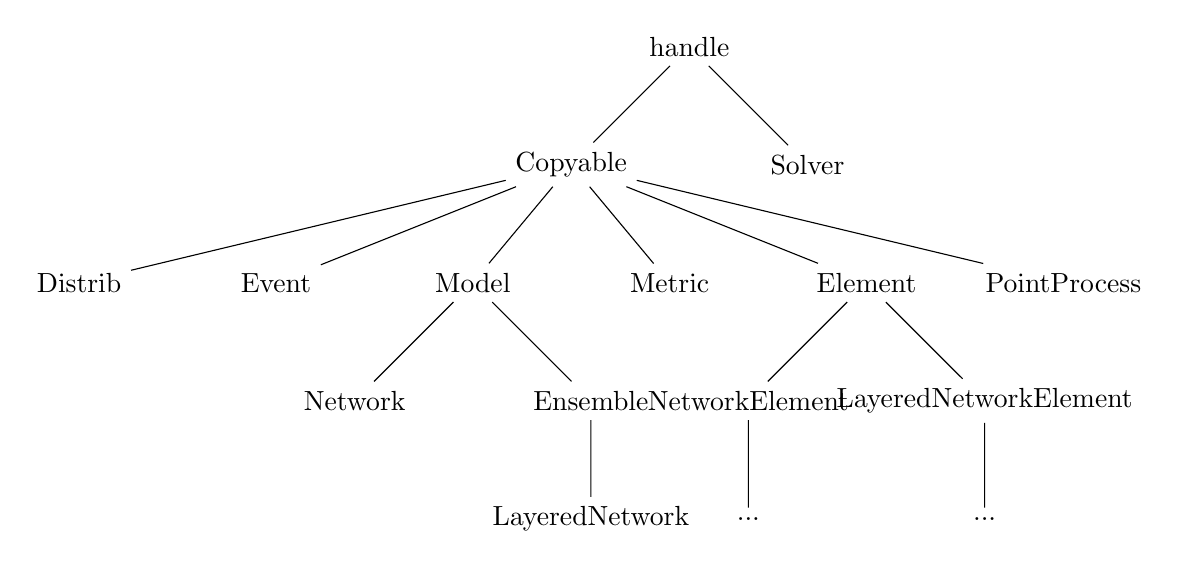
\begin{tikzpicture}[
level 1/.style={sibling distance=3.0cm},
level 2/.style={sibling distance=2.5cm},
level 3/.style={sibling distance=3.0cm},]
\node  {handle}
    child { node {Copyable}
        child { node {Distrib} }
        child { node {Event} }
        child { node {Model}
            child { node {Network} }
            child { node {Ensemble}
                  child { node {LayeredNetwork} }
            }
        }
        child { node {Metric} }
        child { node {Element}
            child { node {NetworkElement}
            child { node {...} }
            }
            child { node {LayeredNetworkElement}
            child { node {...} }
            }
        }
        child { node {PointProcess} }
    }
        child { node {Solver} } 	;
 \end{tikzpicture}
}
\end{center}
The classes in the diagram are as follows:
\begin{itemize}
\item \texttt{Copyable} allows one to perform deep-copy of objects via the \texttt{copy()} method. The class is needed to ensure reproducible behavior in both MATLAB and Octave.
\item \texttt{Distrib} is an abstract class for statistical distributions.
\item \texttt{Element} is the parent class for all the elements that define a model, such as stations, classes, jobs, etc.
\item \texttt{Ensemble} is a class of models defined by a collection of sub-models.
\item \texttt{Event} is a class to describe a generic event occurring in a model, such as an arrival or a departure of a job. This class is used in particular in the \texttt{CTMC} and \texttt{SSA} solvers.
\item \texttt{LayeredNetwork} defines a layered queueing network model.
\item \texttt{Metric} defines an output metric, such as a performance index.
\item \texttt{Reward} is a static class providing reward function templates for CTMC analysis.
\item \texttt{Model} is the parent class for all \textsc{Line} models.
\item \texttt{Network} defines an extended queueing network model.
\item \texttt{NetworkElement} defines an element in a \texttt{Network} model. The sub-hierarchy is detailed in Section~\ref{networkelement-class}.
\item \texttt{LayeredNetworkElement} defines a generic element of a \texttt{LayeredNetwork} model. The sub-hierarchy is expanded in Section~\ref{layerednetworkelement-class}.
\item \texttt{PointProcess} is an abstract class for stochastic point processes (e.g., arrival processes, service processes).
\item \texttt{Solver} is an abstract class for model solution algorithms and tools.
\end{itemize}

\section{NetworkElement class}
\label{networkelement-class}
\begin{center}
{\tiny
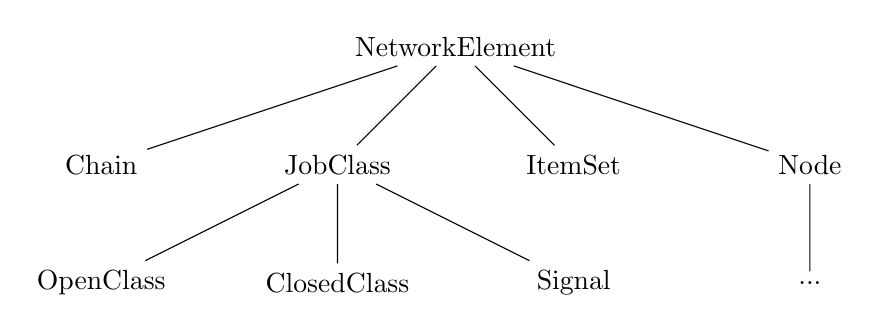
\begin{tikzpicture}[
level 1/.style={sibling distance=3cm},
level 2/.style={sibling distance=3.0cm},
level 3/.style={sibling distance=3.0cm}]
\node {NetworkElement}
                child { node {Chain}}
                child { node {JobClass}
                    child {node {OpenClass}}
                    child {node {ClosedClass}}
                    child {node {Signal}}}
                child { node {ItemSet}}
                child { node {Node}
                    child { node {...} }}
    ;
 \end{tikzpicture}
}
\end{center}
The classes in the diagram are as follows:
\begin{itemize}
\item \texttt{Chain} describes a routing chain, i.e., a collection of classes in which the job can switch its current class.
\item \texttt{JobClass} is an abstract class to describe the class of a job.
\item \texttt{OpenClass} is a class to specify an open class of jobs that arrive from a \texttt{Source} object.
\item \texttt{ClosedClass} allows one to specify a closed class of jobs that perpetually cycle within a system.
\item \texttt{Signal} extends \texttt{JobClass} and represents a signal class for G-network negative customers.
\item \texttt{ItemSet} is a class used to specify a set of cacheable items.
\item \texttt{Node} is an abstract class to describe a resource that can be visited within a network.
\item \texttt{FiniteCapacityRegion} represents a finite capacity constraint over a group of stations.
\end{itemize}

\section{LayeredNetworkElement class}
\label{layerednetworkelement-class}
\begin{center}
{\tiny
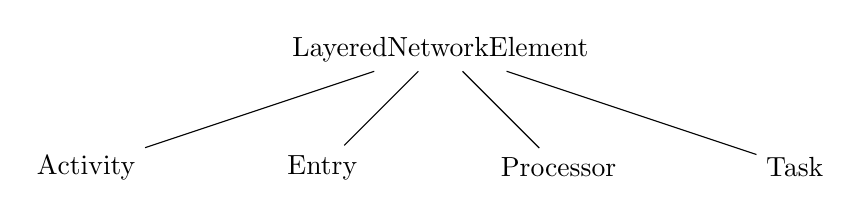
\begin{tikzpicture}[
level 1/.style={sibling distance=3.0cm},
level 2/.style={sibling distance=3.0cm},
level 3/.style={sibling distance=3.0cm},]
\node {LayeredNetworkElement}
                child { node {Activity} }
                child { node {Entry} }
                child { node {Processor} }
                child { node {Task} }
    ;
 	
 \end{tikzpicture}
}
\end{center}
The classes in the diagram are as follows:
\begin{itemize}
\item \texttt{LayeredNetworkElement} abstract class defining a generic element of a \texttt{LayeredNetwork} model.
\item \texttt{Activity} defines a stage of service in a \texttt{Task} of a \texttt{LayeredNetwork}.
\item \texttt{Entry} is a class defining an entry point for service in a \texttt{LayeredNetwork} station.
\item \texttt{Processor} defines a hardware station in a \texttt{LayeredNetwork} model.
\item \texttt{Task} defines a software station in a \texttt{LayeredNetwork} model.
\end{itemize}

\section{Node class}
\begin{center}
{\tiny
\begin{tikzpicture}[sibling distance=7.5em]
\node {NetworkElement}
    child { node {Node}
            child {node {ClassSwitch}}
            child {node {Fork}}
            child {node {Logger}}
            child {node {Router}}
            child {node {Sink}}
            child {node {StatefulNode}
                child {node {...}}
                    }
    };
 	
 \end{tikzpicture}
}
\end{center}
The classes in the diagram are as follows:
\begin{itemize}
\item \texttt{Node} is an abstract class to describe a resource that can be visited within a network.
\item \texttt{ClassSwitch} instantiates a node where jobs switch classes.
\item \texttt{Fork} instantiates a node where jobs are forked into tasks.
\item \texttt{Logger} instantiates a node where jobs are logged upon passage.
\item \texttt{Router} instantiates a node where jobs are routed to other nodes.
\item \texttt{Sink} instantiates a node where jobs in open classes depart the model.
\item \texttt{StatefulNode} is an abstract class describing a node which associated state variables.
\end{itemize}

\section{StatefulNode class}
\begin{center}
{\tiny
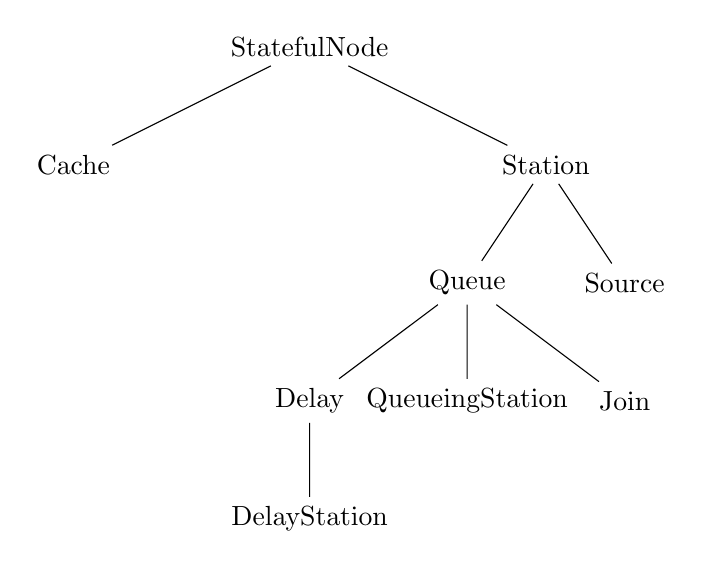
\begin{tikzpicture}[
level 1/.style={sibling distance=6cm},
level 2/.style={sibling distance=2.0cm},
level 3/.style={sibling distance=2.0cm},
level 4/.style={sibling distance=2.0cm},
level 5/.style={sibling distance=2.0cm},]
\node {StatefulNode}
                child {node {Cache}}
                child {node {Station}
                    child {node {Queue}
                        child {node {Delay}
                            child {node {DelayStation}}
                        }
                        child {node {QueueingStation}}
                        child {node {Join}}
                }
                    child {node {Source}}
    };
 	
 \end{tikzpicture}
}
\end{center}
The classes in the diagram are as follows:
\begin{itemize}
\item \texttt{StatefulNode} is an abstract class describing a node which associated state variables.
\item \texttt{Cache} instantiates a cache node.
\item \texttt{Station} is an abstract class for nodes where jobs spend time.
\item \texttt{Join} instantiates a join station.
\item \texttt{Queue} instantiates a queueing station.
\item \texttt{Delay} instantiates a delay station.
\item \texttt{DelayStation} alias for \texttt{Delay}.
\item \texttt{QueueingStation} alias for \texttt{Queue}.
\item \texttt{Source} instantiates a source from which jobs can arrive in open classes.
\item \texttt{ServerType} defines heterogeneous server types within a Queue, enabling different servers with distinct service rates and job class compatibilities.
\end{itemize}

\section{Distrib class}
\begin{center}
{\tiny
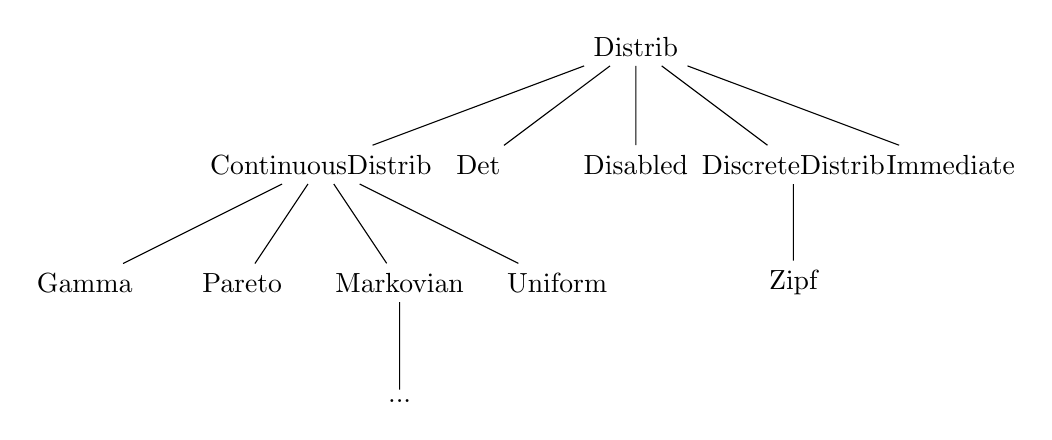
\begin{tikzpicture}[
level 1/.style={sibling distance=2cm},
level 2/.style={sibling distance=2cm},
level 3/.style={sibling distance=2.0cm},
level 4/.style={sibling distance=2.0cm},
level 5/.style={sibling distance=2.0cm},]
\node {Distrib}
            child {node {ContinuousDistrib}
                child {node {Gamma}}
                child {node {Pareto}}
                child {node {Markovian}
                    child {node {...}}
                }
                child {node {Uniform}}
            }
            child {node {Det}}
            child {node {Disabled}}
            child {node {DiscreteDistrib}
                child {node {Zipf}}
            }
            child {node {Immediate}}
            ;
 	
 \end{tikzpicture}
}
\end{center}
The classes in the diagram are as follows:
\begin{itemize}
\item \texttt{Distrib} is an abstract class for statistical distributions.
\item \texttt{ContinuousDistrib} is an abstract class for distributions defined over a continuous interval.
\item \texttt{Det} instantiates a deterministic distribution.
\item \texttt{Disabled} is a placeholder class for a distribution that is disabled or unspecified.
\item \texttt{DiscreteDistrib} is an abstract class for distributions defined at discrete point.
\item \texttt{Zipf} defines a Zipf distribution.
\item \texttt{Immediate} defines a deterministic distribution with mass entirely at 0.
\item \texttt{Pareto} defines a Pareto distribution.
\item \texttt{Markovian} is an abstract class for phase-type distributions.
\item \texttt{Uniform} defines a uniform distribution over a bounded range.
\item \texttt{Prior} extends \texttt{Distribution} and represents a prior distribution for Bayesian parameter uncertainty.
\end{itemize}

\section{Markovian class}
\begin{center}
{\tiny
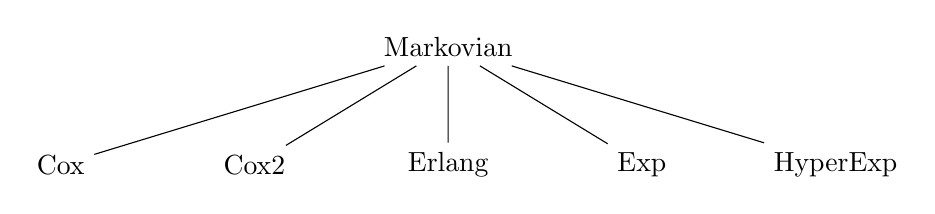
\begin{tikzpicture}[sibling distance=7em]
\node {Markovian}
        child {node {Cox}}
        child {node {Cox2}}
        child {node {Erlang}}
        child {node {Exp}}
        child {node {HyperExp}}
             ; 	
 \end{tikzpicture}
}
\end{center}
The classes in the diagram are as follows:
\begin{itemize}
\item \texttt{Markovian} is an abstract class for phase-type distributions.
\item \texttt{Cox} is a class for Coxian distributions with arbitrary number of phases.
\item \texttt{Cox2} is a class for 2-phase Coxian distributions.
\item \texttt{Erlang} is a class for Erlang distributions with arbitrary number of phases.
\item \texttt{Exp} instantiates an exponential distribution.
\item \texttt{HyperExp} is a class for 2-phase hyper-exponential distributions.
\end{itemize}

\section{PointProcess class}
\begin{center}
{\tiny
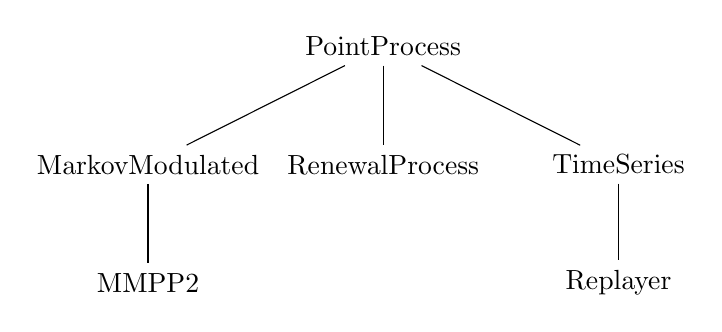
\begin{tikzpicture}[sibling distance=8.5em]
\node {PointProcess}
            child {node {MarkovModulated}
                child {node {MMPP2}}
                }
            child {node {RenewalProcess}}
            child {node {TimeSeries}
                child {node {Replayer}}
                }
             ;
 	
 \end{tikzpicture}
}
\end{center}
The classes in the diagram are as follows:
\begin{itemize}
\item \texttt{PointProcess} is an abstract class for stochastic point processes (e.g., arrival processes, service processes).
\item \texttt{MarkovModulated} is an abstract class for Markov-modulated point processes.
\item \texttt{MMPP2} instantiates a Markov-Modulation Poisson Process with 2-states.
\item \texttt{RenewalProcess} is a class to instantiate processes with i.i.d. samples from an object that inherits from \texttt{Distrib}
\item \texttt{TimeSeries} is an abstract class for empirical point processes.
\item \texttt{Replayer} is a class that loads a time series from a file. \texttt{Trace} is an alias for \texttt{Replayer}.
\end{itemize}

\section{Section class}
\begin{center}
{\tiny
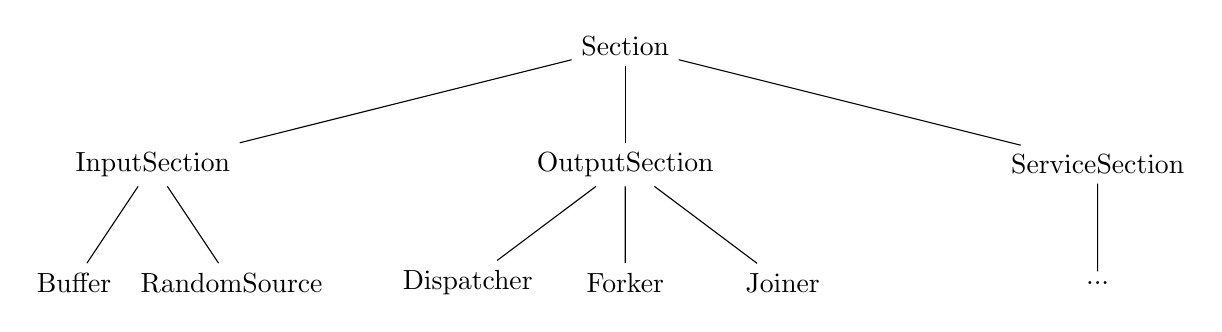
\begin{tikzpicture}[
level 1/.style={sibling distance=6cm},
level 2/.style={sibling distance=2.0cm},
level 3/.style={sibling distance=2.0cm},
level 4/.style={sibling distance=2.0cm},
level 5/.style={sibling distance=2.0cm},]
\node  {Section}
                child {node {InputSection}
                    child {node {Buffer}}
                    child {node {RandomSource}}}
                child {node {OutputSection}
                    child {node {Dispatcher}}
                    child {node {Forker}}
                    child {node {Joiner}}}
                child {node {ServiceSection}
                    child {node {...}}}
             ;
 	
 \end{tikzpicture}
}
\end{center}
The classes in the diagram are as follows:
\begin{itemize}
\item \texttt{Section} is an abstract class defining a section part of a node.
\item \texttt{InputSection} is an abstract class for sections defining the handling of jobs waiting to be served.
\item \texttt{Buffer} is a class defining a waiting buffer.
\item \texttt{RandomSource} is a class defining the generation of jobs in open classes.
\item \texttt{OutputSection} is an abstract class for sections defining the node behaviour after completing service.
\item \texttt{Dispatcher} is a class implementing routing towards another node.
\item \texttt{Forker} is a section forking a job into a set of sibling tasks.
\item \texttt{Joiner} is a section merging sibling tasks into the original job.
\item \texttt{ServiceSection} is an abstract class for sections defining the node behaviour during service.
\end{itemize}

\section{ServiceSection class}
\begin{center}
{\tiny
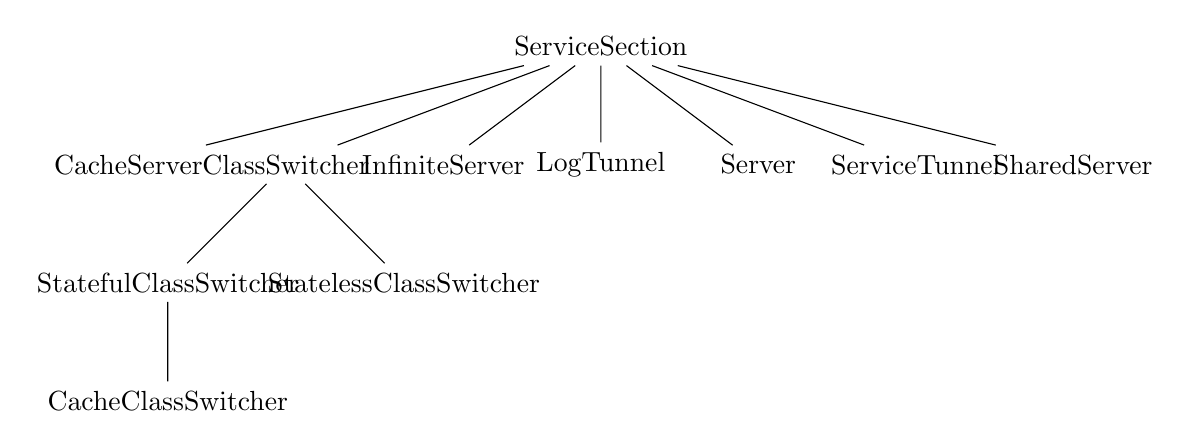
\begin{tikzpicture}[
level 1/.style={sibling distance=2cm},
level 2/.style={sibling distance=3.0cm},
level 3/.style={sibling distance=2.5cm},
level 4/.style={sibling distance=2.5cm},
level 5/.style={sibling distance=2.0cm},]
\node {ServiceSection}
            child {node {CacheServer}}
            child {node {ClassSwitcher}
                child {node {StatefulClassSwitcher}
                   child {node {CacheClassSwitcher}}
                }
                child {node {StatelessClassSwitcher}}
            }
            child {node {InfiniteServer}}
            child {node {LogTunnel}}
            child {node {Server}}
            child {node {ServiceTunnel}}
            child {node {SharedServer}}
            ;
 	
 \end{tikzpicture}
}
\end{center}
The classes in the diagram are as follows:
\begin{itemize}
\item \texttt{ServiceSection} is an abstract class for sections defining the node behaviour during service.
\item \texttt{CacheServer} is a section tracking and updating the cache state.
\item \texttt{ClassSwitcher} is an abstract class for sections changing the class of a visiting job or task.
\item \texttt{StatefulClassSwitcher} is an abstract class for \texttt{ClassSwitcher} sections that depend on the node state.
\item \texttt{CacheClassSwitcher} is a \texttt{StatefulClassSwitcher} that depends on the cache state.
\item \texttt{StatelessClassSwitcher} is an abstract class for \texttt{ClassSwitcher} sections that depend on a static rule.
\item \texttt{InfiniteServer} is a section for non-preemptive service with an infinite level of parallelism.
\item \texttt{LogTunnel} is a dummy service section for \texttt{Logger} nodes.
\item \texttt{Server} is a section for non-preemptive service with a finite level of parallelism. This section includes serial service as a special case.
\item \texttt{ServiceTunnel} is a dummy service section for nodes that do not serve jobs.
\item \texttt{SharedServer} is a section for preemptive service (e.g., processor sharing)
\end{itemize}

\section{Solver class}
\begin{center}
{\tiny
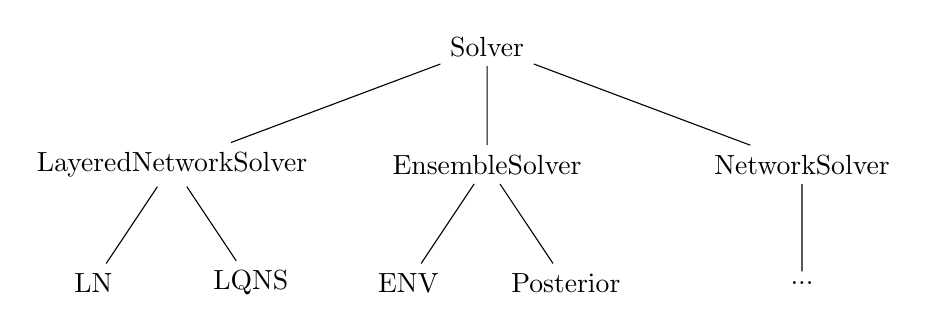
\begin{tikzpicture}[
level 1/.style={sibling distance=4cm},
level 2/.style={sibling distance=2.0cm},
level 3/.style={sibling distance=2.0cm},
level 4/.style={sibling distance=2.5cm},
level 5/.style={sibling distance=2.0cm},]
\node  {Solver}
        child { node {LayeredNetworkSolver}
            child { node {LN} }
            child { node {LQNS} }
        }
        child { node {EnsembleSolver}
            child { node {ENV} }
            child { node {Posterior} }
        }
        child { node {NetworkSolver}
            child { node {...} }
        }
    ;
 	
 \end{tikzpicture}
}
\end{center}
The classes in the diagram are as follows:
\begin{itemize}
\item \texttt{Solver} is an abstract class for model solution algorithms and tools.
\item \texttt{LayeredNetworkSolver} is an abstract class for solvers of \texttt{LayeredNetwork} models.
\item \texttt{LN} implements the \texttt{LN} layered queueing network solver.
\item \texttt{LQNS} implements the interface to the \texttt{LQNS} layered queueing network solver.
\item \texttt{EnsembleSolver}  is an abstract class for solvers of models with random environments.
\item \texttt{ENV} implements the \texttt{Env} random environment solver.
\item \texttt{Posterior} extends \texttt{EnsembleSolver} and is a meta-solver for models with Prior distributions.
\item \texttt{NetworkSolver} is an abstract class for solvers of \texttt{Network} models.
\end{itemize}

\section{NetworkSolver class}
\begin{center}
{\tiny
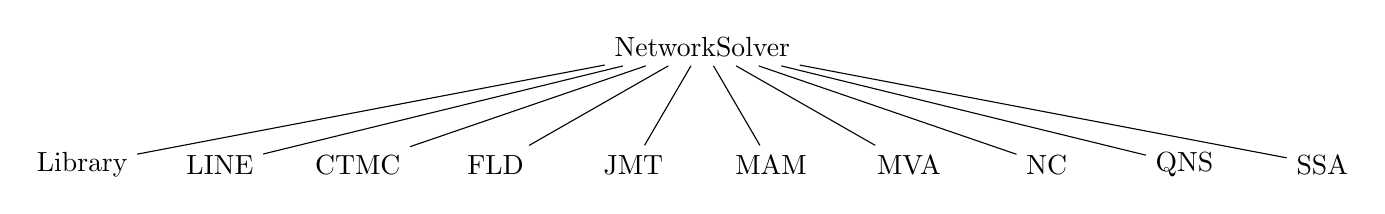
\begin{tikzpicture}[
level 1/.style={sibling distance=1.75cm},
level 2/.style={sibling distance=2.0cm},
level 3/.style={sibling distance=2.0cm},
level 4/.style={sibling distance=2.5cm},
level 5/.style={sibling distance=2.0cm},]
\node  {NetworkSolver}
            child { node {Library} }
            child { node {LINE} }
            child { node {CTMC} }
            child { node {FLD} }
            child { node {JMT} }
            child { node {MAM} }
            child { node {MVA} }
            child { node {NC} }
            child { node {QNS} }
            child { node {SSA} }

    ;
 	
 \end{tikzpicture}
}
\end{center}
The classes in the diagram are as follows:
\begin{itemize}
\item \texttt{NetworkSolver} is the abstract class defining a generic solver for extended queueing network.
\item \texttt{Library} collection of ad-hoc solution methods for extended queueing networks.
\item \texttt{LINE} instantiates a meta-solver that recommends the solver to run for a given model.
\item \texttt{CTMC} instantiates the \texttt{CTMC} solver.
\item \texttt{JMT} instantiates the \texttt{JMT} solver.
\item \texttt{MAM} instantiates the \texttt{MAM} solver.
\item \texttt{MVA} instantiates the \texttt{MVA} solver.
\item \texttt{NC} instantiates the \texttt{NC} solver.
\item \texttt{QNS} instantiates \texttt{LQNS}'s qnsolver.
\item \texttt{SSA} instantiates the \texttt{SSA} solver.
\end{itemize}    
\end{comment}

\chapter{API Function Reference}
\label{ch:api-function-reference}

This appendix provides a comprehensive catalog of all API functions available in the \texttt{jline.api} package. The table lists each function name, its organizational package, and a brief description of its purpose.

\begin{footnotesize}
\begin{longtable}{|p{0.4\linewidth}|p{0.1\linewidth}|p{0.5\linewidth}|}
\caption{Complete API Function Reference}
\label{tab:api-functions}
\\\hline
\textbf{Function Name} & \textbf{Package} & \textbf{Description}
\\\hline
\endfirsthead
\multicolumn{3}{c}%
{\tablename\ \thetable\ -- API Function Reference.\textit{ Continued from previous page}} \\
\hline
\textbf{Function Name} & \textbf{Package} & \textbf{Description}\\
\hline
\endhead
\hline \multicolumn{3}{r}{\textit{Continued on next page}} \\
\endfoot
\hline
\endlastfoot
\texttt{amap2\_fit\_gamma} & mam & Fits AMAP(2) distributions to match moments and correlation characteristics\\
\texttt{amap2\_fit\_gamma\_map} & mam & Fits AMAP(2) by approximating arbitrary-order MAP with preserved correlation structure\\
\texttt{amap2\_fit\_gamma\_trace} & mam & Fits AMAP(2) from empirical traces while preserving autocorrelation characteristics\\
\texttt{aph2\_adjust} & mam & Adjusts moments to ensure feasibility bounds for APH(2) fitting procedures\\
\texttt{aph2\_assemble} & mam & Constructs APH(2) transition matrices from specified rates and transition probabilities\\
\texttt{aph2\_fit} & mam & Fits APH(2) distributions to match given moments with automatic feasibility adjustment\\
\texttt{aph2\_fit\_map} & mam & Fits APH(2) distributions by approximating arbitrary-order MAP processes\\
\texttt{aph2\_fit\_trace} & mam & Fits APH(2) distributions from empirical inter-arrival time traces\\
\texttt{aph2\_fitall} & mam & Fits multiple APH(2) distributions to match given moments with exhaustive parameter search\\
\texttt{aph\_bernstein} & mam & Constructs APH distributions using Bernstein exponential approximation methods\\
\texttt{aph\_fit} & mam & Fits APH distributions to specified moments using optimization and approximation techniques\\
\texttt{aph\_rand} & mam & APH random generation algorithms\\
\texttt{aph\_simplify} & mam & Simplifies and combines APH distributions using structural pattern operations\\
\texttt{cache\_erec} & cache & Implements exact recursive (EREC) algorithms for cache system analysis\\
\texttt{cache\_gamma} & cache & Computes cache access factors from request arrival rates and routing matrices\\
\texttt{cache\_gamma\_lp} & cache & Computes cache access factors using linear programming optimization methods\\
\texttt{cache\_miss} & cache & Provides general-purpose algorithms for computing cache miss rates across\\
\texttt{cache\_miss\_asy} & cache & Provides asymptotic approximation methods for cache miss rate analysis\\
\texttt{cache\_miss\_fpi} & cache & Computes cache miss probabilities using fixed-point iteration methods\\
\texttt{cache\_miss\_rayint} & cache & Estimates cache miss rates using ray method for partial differential equations\\
\texttt{cache\_mva} & cache & Implements Mean Value Analysis algorithms for cache system performance\\
\texttt{cache\_mva\_miss} & cache & Implements Mean Value Analysis (MVA) algorithms for computing cache miss\\
\texttt{cache\_prob\_erec} & cache & Computes exact cache state probabilities using recursive methods based on\\
\texttt{cache\_prob\_fpi} & cache & Computes cache state probabilities using fixed-point iteration algorithms\\
\texttt{cache\_prob\_rayint} & cache & Computes cache state probabilities using ray integration methods for\\
\texttt{cache\_rayint} & cache & Implements ray integration techniques for cache system analysis using\\
\texttt{cache\_rrm\_meanfield\_ode} & cache & Implements the mean field ordinary differential equation system for Random\\
\texttt{cache\_t\_hlru} & cache & Computes response time metrics for Hierarchical Least Recently Used (H-LRU)\\
\texttt{cache\_t\_lrum} & cache & Computes response time metrics for Least Recently Used with Multiple servers\\
\texttt{cache\_t\_lrum\_map} & cache & Analyzes response times for LRUM cache systems with Markovian Arrival\\
\texttt{cache\_ttl\_hlru} & cache & Implements TTL approximation for Hierarchical LRU (H-LRU) cache systems\\
\texttt{cache\_ttl\_lrua} & cache & Implementation of Time-To-Live (TTL) approximation for LRU(A) cache systems\\
\texttt{cache\_ttl\_lrum} & cache & Implementation of Time-To-Live approximation for Least Recently Used with\\
\texttt{cache\_ttl\_lrum\_map} & cache & Combines TTL approximation with LRUM cache policies and Markovian Arrival\\
\texttt{cache\_ttl\_tree} & cache & Tree-based TTL cache analysis implementation for the LINE solver framework\\
\texttt{cache\_xi\_bvh} & cache & Computes cache xi terms using the iterative method from Gast-van Houdt\\
\texttt{cache\_xi\_fp} & cache & Estimates cache xi terms using fixed-point algorithms. Xi terms represent\\
\texttt{ctmc\_courtois} & mc & Courtois decomposition for nearly completely decomposable CTMCs\\
\texttt{ctmc\_kms} & mc & Koury-McAllister-Stewart aggregation-disaggregation method for CTMCs\\
\texttt{ctmc\_makeinfgen} & mc & Constructs and validates infinitesimal generator matrices for continuous-time\\
\texttt{ctmc\_multi} & mc & Multi-level aggregation method for CTMCs\\
\texttt{ctmc\_pseudostochcomp} & mc & API function for mc operations\\
\texttt{ctmc\_rand} & mc & Generates random infinitesimal generator matrices for continuous-time Markov chains\\
\texttt{ctmc\_randomization} & mc & Converts a continuous-time Markov chain into an equivalent discrete-time chain\\
\texttt{ctmc\_relsolve} & mc & Equilibrium distribution of a continuous-time Markov chain re-normalized with respect to\\
\texttt{ctmc\_simulate} & mc & Generates sample paths for CTMCs using the standard simulation algorithm with\\
\texttt{ctmc\_solve} & mc & Computes the steady-state probability distribution for CTMCs by solving the linear\\
\texttt{ctmc\_solve\_reducible} & mc & Solve reducible CTMCs by converting to DTMC via randomization\\
\texttt{ctmc\_ssg} & mc & API function for mc operations\\
\texttt{ctmc\_ssg\_reachability} & mc & CTMC State Space Generator for Reachability Analysis\\
\texttt{ctmc\_stmonotone} & mc & Computes the stochastically monotone upper bound for a CTMC\\
\texttt{ctmc\_stochcomp} & mc & Implements stochastic complementarity analysis for CTMCs to identify strongly\\
\texttt{ctmc\_takahashi} & mc & Takahashi's aggregation-disaggregation method for CTMCs\\
\texttt{ctmc\_testpf\_kolmogorov} & mc & Test if a CTMC has product form using Kolmogorov's criteria\\
\texttt{ctmc\_timereverse} & mc & Computes the infinitesimal generator of the time-reversed continuous-time\\
\texttt{ctmc\_transient} & mc & Computes transient probabilities for CTMCs using numerical integration of the\\
\texttt{ctmc\_uniformization} & mc & CTMC Transient Analysis via Uniformization\\
\texttt{dtmc\_isfeasible} & mc & Check if a matrix represents a feasible DTMC transition matrix\\
\texttt{dtmc\_makestochastic} & mc & Converts non-negative matrices into valid discrete-time Markov chain transition\\
\texttt{dtmc\_rand} & mc & Generates random stochastic transition matrices for discrete-time Markov chains\\
\texttt{dtmc\_simulate} & mc & Generates sample trajectories for DTMCs by sampling from the transition probability\\
\texttt{dtmc\_solve} & mc & Computes the steady-state probability distribution for DTMCs by converting the\\
\texttt{dtmc\_solve\_reducible} & mc & Result class for DTMC solve reducible\\
\texttt{dtmc\_stochcomp} & mc & Returns the stochastic complement of a DTMC\\
\texttt{dtmc\_timereverse} & mc & Compute the infinitesimal generator of the time-reversed DTMC\\
\texttt{dtmc\_uniformization} & mc & Result class for DTMC uniformization analysis containing the probability vector and maximum iterations used\\
\texttt{lossn\_erlangfp} & lossn & Implements fixed-point algorithms for analyzing loss networks using Erlang\\
\texttt{lsn\_max\_multiplicity} & lsn & Computes maximum multiplicity constraints for load sharing network (LSN)\\
\texttt{m3pp22\_fitc\_approx\_cov} & mam.m3pp & Implements parameter fitting for second-order Marked Markov Modulated Poisson Process\\
\texttt{m3pp22\_fitc\_approx\_cov\_multiclass} & mam.m3pp & Implements constrained optimization for fitting M3PP(2,2) parameters given an underlying\\
\texttt{m3pp22\_interleave\_fitc} & mam.m3pp & Implements lumped superposition of multiple M3PP(2,2) processes using interleaved\\
\texttt{m3pp2m\_fitc} & mam.m3pp & Implements exact fitting of second-order Marked Markov Modulated Poisson Process\\
\texttt{m3pp2m\_fitc\_approx} & mam.m3pp & Implements approximation-based fitting for M3PP(2,m) using optimization methods\\
\texttt{m3pp2m\_fitc\_approx\_ag} & mam.m3pp & Implements auto-gamma approximation method for M3PP(2,m) parameter fitting\\
\texttt{m3pp2m\_fitc\_approx\_ag\_multiclass} & mam.m3pp & Implements multiclass auto-gamma fitting for M3PP(2,m) with variance and covariance\\
\texttt{m3pp2m\_interleave} & mam.m3pp & Implements interleaved superposition of multiple M3PP(2,m) processes to construct\\
\texttt{m3pp\_interleave\_fitc} & mam.m3pp & Implements fitting and interleaving of k second-order M3PP processes with varying\\
\texttt{m3pp\_interleave\_fitc\_theoretical} & mam.m3pp & Implements theoretical MMAP fitting through M3PP interleaving using analytical\\
\texttt{m3pp\_interleave\_fitc\_trace} & mam.m3pp & Implements M3PP interleaving and fitting directly from empirical trace data\\
\texttt{m3pp\_rand} & mam.m3pp & Implements random generation of Markovian Multi-class Point Processes (M3PP)\\
\texttt{m3pp\_superpos\_fitc} & mam.m3pp & Implements superposition-based fitting of k second-order M3PP processes into\\
\texttt{m3pp\_superpos\_fitc\_theoretical} & mam.m3pp & Implements superposition fitting of k second-order M3PP processes using theoretical\\
\texttt{mamap22\_fit\_gamma\_fs\_trace} & mam & Fits MAMAP(2,2) from trace data using gamma autocorrelation and forward-sigma characteristics\\
\texttt{mamap22\_fit\_multiclass} & mam & Fits MAMAP(2,2) processes for two-class systems with forward moments and sigma characteristics\\
\texttt{mamap2m\_coefficients} & mam & Computes coefficients for MAMAP(2,m) fitting formulas in canonical forms\\
\texttt{mamap2m\_fit} & mam & Fits MAMAP(2,m) processes matching moments, autocorrelation, and class characteristics\\
\texttt{mamap2m\_fit\_fb\_multiclass} & mam & Fits MAMAP using combined forward and backward moment characteristics for multiclass systems\\
\texttt{mamap2m\_fit\_gamma\_fb\_mmap} & mam & Fits MAMAP with autocorrelation control using forward-backward moments from MMAP input\\
\texttt{mamap2m\_fit\_mmap} & mam & Fits MAPH/MAMAP(2,m) by approximating characteristics of input MMAP processes\\
\texttt{mamap2m\_fit\_trace} & mam & Fits MAMAP(2,m) processes from empirical trace data with inter-arrival times and class labels\\
\texttt{map2\_fit} & mam & Fits MAP(2) processes to match specified moments and autocorrelation decay rates\\
\texttt{map2mmpp} & mam & Converts MAP representations to MMPP format for compatibility with MMPP-specific algorithms\\
\texttt{map\_acf} & mam & Computes autocorrelation function (ACF) values for MAP inter-arrival times at specified lags\\
\texttt{map\_acfc} & mam & Computes ACFC values for MAP counting processes over time intervals, measuring temporal correlation\\
\texttt{map\_block} & mam & Constructs MAP(2) representations from moment and autocorrelation parameters using fallback\\
\texttt{map\_ccdf\_derivative} & mam & Computes derivatives of MAP complementary cumulative distribution functions at zero\\
\texttt{map\_cdf} & mam & Computes CDF values for MAP inter-arrival times using CTMC uniformization techniques\\
\texttt{map\_checkfeasible} & mam & Comprehensive validation of MAP matrices including stochastic properties, numerical stability,\\
\texttt{map\_count\_mean} & mam & Computes mean number of arrivals in MAP counting processes over specified time intervals\\
\texttt{map\_count\_moment} & mam & Computes power moments of MAP counting processes using moment generating functions and\\
\texttt{map\_count\_var} & mam & Computes variance of MAP counting processes over specified time intervals using matrix\\
\texttt{map\_embedded} & mam & Computes embedded DTMC matrices from MAP representations by extracting transition\\
\texttt{map\_erlang} & mam & Constructs MAP representations of Erlang-k processes with specified means and phases\\
\texttt{map\_exponential} & mam & Creates MAP representations of exponential inter-arrival time distributions with specified\\
\texttt{map\_feasblock} & mam & Constructs feasible MAP representations when exact moment matching fails by adjusting\\
\texttt{map\_feastol} & mam & Provides standard tolerance values for numerical feasibility checks in MAP algorithms\\
\texttt{map\_gamma} & mam & Computes gamma parameter measuring autocorrelation decay rates in MAP processes\\
\texttt{map\_gamma2} & mam & Computes largest non-unit eigenvalue of embedded DTMC for MAP correlation characterization\\
\texttt{map\_hyperexp} & mam & Constructs MAP representations of two-phase hyperexponential renewal processes\\
\texttt{map\_idc} & mam & Computes asymptotic index of dispersion for MAP counting processes, measuring long-term\\
\texttt{map\_infgen} & mam & Computes infinitesimal generator matrix of underlying CTMC by combining MAP transition\\
\texttt{map\_isfeasible} & mam & Provides convenient interface for MAP feasibility validation with configurable tolerance\\
\texttt{map\_joint} & mam & Computes joint moments of MAP inter-arrival times for advanced statistical characterization\\
\texttt{map\_jointpdf\_derivative} & mam & Computes partial derivatives of MAP joint probability density functions at origin\\
\texttt{map\_kpc} & mam & Computes Kronecker product composition of multiple MAPs for building complex arrival processes\\
\texttt{map\_kurt} & mam & Computes kurtosis of MAP inter-arrival times measuring tail heaviness and distribution shape\\
\texttt{map\_lambda} & mam & MAP arrival rate computation algorithms\\
\texttt{map\_largemap} & mam & Provides size thresholds for determining when MAP algorithms should switch to\\
\texttt{map\_mark} & mam & Creates Marked MAP (MMAP) representations by adding class labels to MAP arrivals\\
\texttt{map\_max} & mam & Computes MAP representation of maximum inter-arrival times from independent MAP processes\\
\texttt{map\_mean} & mam & MAP mean inter-arrival time computation algorithms\\
\texttt{map\_mixture} & mam & Creates probabilistic mixtures of MAP processes with specified mixture probabilities\\
\texttt{map\_moment} & mam & Computes raw moments of MAP inter-arrival times using matrix inversion techniques\\
\texttt{map\_normalize} & mam & Sanitizes MAP matrices by ensuring non-negativity constraints and proper diagonal adjustments\\
\texttt{map\_pdf} & mam & Computes PDF values for MAP inter-arrival times using matrix exponential techniques\\
\texttt{map\_pie} & mam & Computes steady-state probability vector of embedded discrete-time Markov chain\\
\texttt{map\_piq} & mam & Computes steady-state probability vector of underlying continuous-time Markov chain\\
\texttt{map\_pntiter} & mam & Computes exact arrival probabilities using iterative numerical methods based on Neuts and Li\\
\texttt{map\_pntquad} & mam & Computes MAP point process probabilities using ODE quadrature methods with Runge-Kutta integration\\
\texttt{map\_prob} & mam & Computes equilibrium probability distribution of underlying CTMC for MAP analysis\\
\texttt{map\_rand} & mam & Generates random MAP representations for testing, simulation, and statistical analysis\\
\texttt{map\_randn} & mam & Generates random MAP samples with added numerical noise for robustness testing\\
\texttt{map\_renewal} & mam & Creates renewal MAP by removing correlations to obtain memoryless arrival processes\\
\texttt{map\_sample} & mam & Generates random samples from MAP distributions for simulation and empirical analysis\\
\texttt{map\_scale} & mam & Rescales MAP inter-arrival time distributions to achieve specified mean values\\
\texttt{map\_scv} & mam & Computes SCV of MAP inter-arrival times as normalized dispersion measure\\
\texttt{map\_skew} & mam & Computes skewness of MAP inter-arrival times measuring asymmetry in distributions\\
\texttt{map\_stochcomp} & mam & Performs state elimination through stochastic complementation while preserving MAP properties\\
\texttt{map\_sum} & mam & Computes MAP representations of sums of identical MAP processes for load scaling\\
\texttt{map\_sumind} & mam & Computes MAP representations of sums of independent MAP processes for modeling\\
\texttt{map\_super} & mam & Creates superposition of MAP processes using Kronecker product techniques\\
\texttt{map\_timereverse} & mam & Computes time-reversed MAP by adjusting transition rates based on stationary distributions\\
\texttt{map\_var} & mam & MAP variance computation algorithms\\
\texttt{map\_varcount} & mam & Computes variance of event counts in MAP processes over specified time intervals\\
\texttt{maph2m\_fit} & mam & Fits MAPH(2,m) processes to match ordinary moments, class probabilities, and backward moments\\
\texttt{maph2m\_fit\_mmap} & mam & Fits MAPH(2,m) by approximating characteristics of input MMAP processes\\
\texttt{maph2m\_fit\_multiclass} & mam & Fits MAPH(2,m) models to multiclass characteristics with class-specific parameters\\
\texttt{maph2m\_fit\_trace} & mam & Fits MAPH(2,m) from empirical trace data for multiclass service time modeling\\
\texttt{maph2m\_fitc\_approx} & mam & Fits MAPH(2,m) using approximation methods for count statistics when exact solutions fail\\
\texttt{maph2m\_fitc\_theoretical} & mam & Fits MAPH(2,m) using theoretical count statistics for precise parameter estimation\\
\texttt{mapqn\_bnd\_lr} & mapqn & Implements general linear reduction methods for computing performance\\
\texttt{mapqn\_bnd\_lr\_mva} & mapqn & Implements linear reduction bounds for MAP queueing networks using Mean\\
\texttt{mapqn\_bnd\_lr\_pf} & mapqn & Implements linear reduction bounds specialized for product-form MAP\\
\texttt{mapqn\_bnd\_qr} & mapqn & Implements general quadratic reduction methods for computing performance\\
\texttt{mapqn\_bnd\_qr\_delay} & mapqn & Implements quadratic reduction bounds for delay systems in MAP queueing\\
\texttt{mapqn\_bnd\_qr\_ld} & mapqn & Implements quadratic reduction bounds for load-dependent MAP queueing\\
\texttt{mapqn\_lpmodel} & mapqn & Base class for representing MAP queueing network linear programming models\\
\texttt{mapqn\_parameters} & mapqn & Defines the base parameter structure for MAP queueing network analysis\\
\texttt{mapqn\_parameters\_factory} & mapqn & Factory class for creating parameter objects for MAP queueing network\\
\texttt{mapqn\_qr\_bounds\_bas} & mapqn & Implements Queue-Router bounds using the Balanced Asymptotic Scaling (BAS)\\
\texttt{mapqn\_qr\_bounds\_rsrd} & mapqn & Implements Queue-Router (QR) bounds using the Randomized Simultaneous\\
\texttt{mmap\_backward\_moment} & mam & Computes backward moments of MMAP inter-arrival times for each marked class\\
\texttt{mmap\_compress} & mam & Compresses MMAP using various approximation methods including mixture, matching,\\
\texttt{mmap\_count\_idc} & mam & Computes IDC values for each marked class in MMAP counting processes\\
\texttt{mmap\_count\_lambda} & mam & Computes arrival rate vectors for each marked class in MMAP processes\\
\texttt{mmap\_count\_mcov} & mam & Computes count covariance matrices between marked classes in MMAP processes\\
\texttt{mmap\_count\_mean} & mam & Computes mean count vectors for each marked class in MMAP counting processes\\
\texttt{mmap\_count\_var} & mam & Computes variance vectors for counting processes of each marked class in MMAP\\
\texttt{mmap\_cross\_moment} & mam & Computes cross-moment matrices between different marked classes in MMAP processes\\
\texttt{mmap\_embedded} & mam & Computes embedded discrete-time Markov chain for MMAP processes\\
\texttt{mmap\_exponential} & mam & Constructs MMAP with exponential inter-arrival distributions for each marked class\\
\texttt{mmap\_forward\_moment} & mam & Computes forward moments of MMAP inter-arrival times for each marked class\\
\texttt{mmap\_hide} & mam & Hides specified arrival classes in MMAP processes by removing observable events\\
\texttt{mmap\_idc} & mam & Computes asymptotic IDC for each marked class in MMAP as time approaches infinity\\
\texttt{mmap\_isfeasible} & mam & Validates mathematical feasibility of MMAP representations including stochastic\\
\texttt{mmap\_issym} & mam & Checks if an MMAP is symmetric\\
\texttt{mmap\_lambda} & mam & MMAP arrival rate computation algorithms\\
\texttt{mmap\_maps} & mam & Extracts individual MAP processes for each marked class from MMAP representations\\
\texttt{mmap\_mark} & mam & Converts a Markovian Arrival Process with marked arrivals (MMAP) into a new MMAP with redefined classes based on a given probability matrix\\
\texttt{mmap\_max} & mam & Computes element-wise maximum of MMAP processes for synchronization analysis\\
\texttt{mmap\_mixture} & mam & Creates probabilistic mixtures of MMAP processes with specified weights\\
\texttt{mmap\_mixture\_fit} & mam & Fits a mixture of Markovian Arrival Processes (MMAPs) to match the given cross-moments\\
\texttt{mmap\_mixture\_fit\_mmap} & mam & Fits a mixture of Markovian Arrival Processes (MMAPs) to match the given moments\\
\texttt{mmap\_mixture\_order2} & mam & Creates a second-order MMAP mixture from a collection of MMAPs\\
\texttt{mmap\_modulate} & mam & Modulates an MMAP by another MMAP, creating a compound arrival process\\
\texttt{mmap\_normalize} & mam & Normalizes MMAP matrices to ensure feasibility and mathematical validity\\
\texttt{mmap\_pc} & mam & Computes the proportion of counts (PC) for each type in a Markovian Arrival Process with marked arrivals (MMAP)\\
\texttt{mmap\_pie} & mam & Computes steady-state probability vectors for each marked class in MMAP processes\\
\texttt{mmap\_rand} & mam & Generates random MMAP representations for testing and simulation purposes\\
\texttt{mmap\_sample} & mam & Generates random samples from MMAP distributions for each marked class\\
\texttt{mmap\_scale} & mam & Rescales MMAP inter-arrival distributions to achieve specified mean values\\
\texttt{mmap\_shorten} & mam & Converts an MMAP representation from M3A format to BUTools format\\
\texttt{mmap\_sigma} & mam & Computes one-step class transition probabilities for a Marked Markovian Arrival Process (MMAP)\\
\texttt{mmap\_sigma2} & mam & Computes two-step class transition probabilities for a Markovian Arrival Process (MMAP)\\
\texttt{mmap\_sum} & mam & Computes superposition of MMAP processes creating independent multiclass arrival streams\\
\texttt{mmap\_super} & mam & Combines multiple MMAP processes into superposed multiclass arrival streams\\
\texttt{mmap\_super\_safe} & mam & API function for mam operations\\
\texttt{mmap\_timereverse} & mam & Computes the time-reversed version of a Markovian Arrival Process with marked arrivals (MMAP)\\
\texttt{mmpp2\_fit} & mam & Fits MMPP(2) models to match specified moments and correlation characteristics\\
\texttt{mmpp2\_fit1} & mam & Fits MMPP(2) models using simplified single-parameter approach for specific scenarios\\
\texttt{mmpp2\_fitc} & mam & Fits MMPP(2) models using count statistics and index of dispersion criteria\\
\texttt{mmpp2\_fitc\_approx} & mam & Fits MMPP(2) using optimization-based approximation methods for count statistics\\
\texttt{mmpp\_rand} & mam & Generates random MMPP models with diagonal D1 matrices for testing and simulation\\
\texttt{ms\_additivesymmetricchisquared} & measures & Additive symmetric chi-squared distance between two probability distributions\\
\texttt{ms\_adtest} & measures & Implements the Anderson-Darling test for assessing whether a sample comes from\\
\texttt{ms\_avgl1linfty} & measures & Average L1 L-infinity distance between two probability distributions\\
\texttt{ms\_bhattacharyya} & measures & Computes the Bhattacharyya distance measuring the similarity between probability\\
\texttt{ms\_canberra} & measures & Canberra distance between two probability distributions\\
\texttt{ms\_chebyshev} & measures & Chebyshev Distance for Probability Distributions\\
\texttt{ms\_chisquared} & measures & Squared chi-squared distance between two probability distributions\\
\texttt{ms\_cityblock} & measures & Implements the City block distance between probability distributions\\
\texttt{ms\_clark} & measures & Clark distance between two probability distributions\\
\texttt{ms\_condentropy} & measures & Computes conditional entropy measuring the remaining uncertainty\\
\texttt{ms\_cramer\_von\_mises} & measures & Implements the Cramer-von Mises test statistic for comparing two empirical distributions\\
\texttt{ms\_cosine} & measures & Computes cosine distance (1 - cosine similarity) measuring the angle between two\\
\texttt{ms\_czekanowski} & measures & Czekanowski distance between two probability distributions\\
\texttt{ms\_dice} & measures & Dice distance between two probability distributions\\
\texttt{ms\_divergence} & measures & Divergence distance between two probability distributions\\
\texttt{ms\_entropy} & measures & Implements Shannon entropy for discrete random variables\\
\texttt{ms\_euclidean} & measures & Implements the standard Euclidean distance between probability distributions\\
\texttt{ms\_fidelity} & measures & Fidelity distance between two probability distributions\\
\texttt{ms\_gower} & measures & Gower distance between two probability distributions\\
\texttt{ms\_harmonicmean} & measures & Harmonic mean distance between two probability distributions\\
\texttt{ms\_hellinger} & measures & Computes the Hellinger distance measuring dissimilarity between probability distributions\\
\texttt{ms\_intersection} & measures & Intersection distance between two probability distributions\\
\texttt{ms\_jaccard} & measures & Jaccard distance between two probability distributions\\
\texttt{ms\_jeffreys} & measures & Jeffreys divergence between two probability distributions\\
\texttt{ms\_jensendifference} & measures & Jensen difference divergence between two probability distributions\\
\texttt{ms\_jensenshannon} & measures & Implements Jensen-Shannon divergence, a symmetric and bounded version of\\
\texttt{ms\_jointentropy} & measures & Computes joint entropy measuring the uncertainty of joint distributions\\
\texttt{ms\_kdivergence} & measures & K-divergence between two probability distributions\\
\texttt{ms\_kolmogorov\_smirnov} & measures & Implements the Kolmogorov-Smirnov test for determining if a sample follows\\
\texttt{ms\_kuiper} & measures & Implements the Kuiper test statistic, a rotation-invariant variant of the Kolmogorov-Smirnov\\
\texttt{ms\_kulczynskid} & measures & Kulczynski d distance between two probability distributions\\
\texttt{ms\_kulczynskis} & measures & Kulczynski s distance between two probability distributions\\
\texttt{ms\_kullbackleibler} & measures & Implements the Kullback-Leibler divergence measuring distribution differences\\
\texttt{ms\_kumarhassebrook} & measures & Kumar-Hassebrook distance between two probability distributions\\
\texttt{ms\_kumarjohnson} & measures & Kumar-Johnson distance between two probability distributions\\
\texttt{ms\_lorentzian} & measures & Lorentzian distance between two probability distributions\\
\texttt{ms\_matusita} & measures & Matusita distance between two probability distributions\\
\texttt{ms\_minkowski} & measures & Minkowski Distance for Probability Distributions\\
\texttt{ms\_motyka} & measures & Motyka distance between two probability distributions\\
\texttt{ms\_mutinfo} & measures & Computes mutual information measuring the amount of shared information\\
\texttt{ms\_neymanchisquared} & measures & Neyman chi-squared distance between two probability distributions\\
\texttt{ms\_nmi} & measures & Computes normalized mutual information providing a scale-invariant measure\\
\texttt{ms\_nvi} & measures & Computes normalized variation information measuring the normalized distance\\
\texttt{ms\_pearsonchisquared} & measures & Pearson chi-squared distance between two probability distributions\\
\texttt{ms\_probsymmchisquared} & measures & Probabilistic symmetry chi-squared distance between two probability distributions\\
\texttt{ms\_relatentropy} & measures & Computes relative entropy measuring the information difference\\
\texttt{ms\_product} & measures & Product distance between two probability distributions\\
\texttt{ms\_ruzicka} & measures & Ruzicka distance between two probability distributions\\
\texttt{ms\_soergel} & measures & Soergel distance between two probability distributions\\
\texttt{ms\_sorensen} & measures & Sorensen distance between two probability distributions\\
\texttt{ms\_squaredchord} & measures & Squared chord distance between two probability distributions\\
\texttt{ms\_squaredeuclidean} & measures & Squared Euclidean distance between two probability distributions\\
\texttt{ms\_taneja} & measures & Taneja distance between two probability distributions\\
\texttt{ms\_tanimoto} & measures & Tanimoto distance between two probability distributions\\
\texttt{ms\_topsoe} & measures & Topsoe distance between two probability distributions\\
\texttt{ms\_wasserstein} & measures & Implements the Wasserstein distance measuring the minimum cost to transform\\
\texttt{ms\_wavehegdes} & measures & Wave-Hedges distance between two probability distributions\\
\texttt{mtrace\_backward\_moment} & trace & Computes backward moments of a multi-class trace\\
\texttt{mtrace\_bootstrap} & trace & Implements bootstrap resampling methods for multi-class empirical trace data\\
\texttt{mtrace\_count} & trace & Computes count statistics from a multi-class trace over specified time windows\\
\texttt{mtrace\_cov} & trace & Computes the covariance matrix for multi-type traces\\
\texttt{mtrace\_cross\_moment} & trace & Computes the k-th order moment of the inter-arrival time between an event\\
\texttt{mtrace\_forward\_moment} & trace & Computes the forward moments of a marked trace\\
\texttt{mtrace\_iat2counts} & trace & Computes the per-class counting processes of T, i.e., the counts after\\
\texttt{mtrace\_joint} & trace & Given a multi-class trace, computes the empirical class-dependent joint\\
\texttt{mtrace\_mean} & trace & Computes per-class means for multi-class empirical trace data. Enables separate\\
\texttt{mtrace\_merge} & trace & Merges two traces in a single marked (multiclass) trace\\
\texttt{mtrace\_moment} & trace & Computes empirical class-dependent statistical moments for multi-class trace data\\
\texttt{mtrace\_moment\_simple} & trace & Computes the k-th order moment of the inter-arrival time between an event\\
\texttt{mtrace\_pc} & trace & Computes the probabilities of arrival for each class\\
\texttt{mtrace\_sigma} & trace & Computes the empirical probability of observing a specific 2-element\\
\texttt{mtrace\_sigma2} & trace & Computes the empirical probability of observing a specific 3-element\\
\texttt{mtrace\_split} & trace & Given a multi-class trace with inter-arrivals T and labels L,\\
\texttt{mtrace\_summary} & trace & Computes summary statistics for multiple trace analysis, providing\\
\texttt{npfqn\_nonexp\_approx} & npfqn & Implements approximation methods for non-product-form queueing networks\\
\texttt{npfqn\_traffic\_merge} & npfqn & Implements traffic merging algorithms for non-product-form queueing networks\\
\texttt{npfqn\_traffic\_merge\_cs} & npfqn & Implements traffic merging algorithms for non-product-form queueing networks\\
\texttt{npfqn\_traffic\_split\_cs} & npfqn & Implements traffic splitting algorithms for non-product-form queueing networks\\
\texttt{pfqn\_ab} & pfqn.ld & Implements the Akyildiz-Bolch linearizer method for analyzing closed product-form queueing networks\\
\texttt{pfqn\_aql} & pfqn.mva & Implements the Aggregate Queue Length (AQL) approximation method for analyzing closed\\
\texttt{pfqn\_bs} & pfqn.mva & Implements the classic Bard-Schweitzer approximate MVA algorithm for closed queueing networks\\
\texttt{pfqn\_ca} & pfqn.nc & Convolution Algorithm for Product-Form Networks\\
\texttt{pfqn\_cdfun} & pfqn.ld & Provides functionality to evaluate class-dependent scaling functions in load-dependent queueing networks\\
\texttt{pfqn\_comomrm} & pfqn.nc & Implements the Convolution Method of Moments specialized for repairman queueing models\\
\texttt{pfqn\_comomrm\_ld} & pfqn.ld & Implements the Convolution Method of Moments (COMOM) for computing normalizing constants in\\
\texttt{pfqn\_conwayms} & pfqn.mva & Implements the Conway-Maxwell approximation method for analyzing closed queueing networks\\
\texttt{pfqn\_cub} & pfqn.nc & Implements the cubature (multi-dimensional integration) approach for computing normalizing\\
\texttt{pfqn\_egflinearizer} & pfqn.mva & Implements the Extended General-Form linearizer approximation for closed queueing networks\\
\texttt{pfqn\_fnc} & pfqn.ld & Computes scaling factors for load-dependent functional servers in product-form queueing networks\\
\texttt{pfqn\_gflinearizer} & pfqn.mva & Implements the general-form linearizer approximation for closed queueing networks with\\
\texttt{pfqn\_gld} & pfqn.ld & Implements the generalized convolution algorithm for computing normalizing constants in\\
\texttt{pfqn\_gld\_complex} & pfqn.ld & Extends the generalized load-dependent convolution algorithm to handle complex-valued\\
\texttt{pfqn\_gldsingle} & pfqn.ld & Provides specialized auxiliary function for computing normalizing constants in single-class\\
\texttt{pfqn\_gldsingle\_complex} & pfqn.ld & Provides specialized auxiliary function for computing normalizing constants in single-class\\
\texttt{pfqn\_kt} & pfqn.nc & Implements the Knessl-Tier asymptotic expansion using the ray method for computing\\
\texttt{pfqn\_le} & pfqn.nc & Implements the Laguerre expansion approach for computing normalizing constants in\\
\texttt{pfqn\_le\_fpi} & pfqn.nc & Implements the fixed-point iteration algorithm used in the Laguerre expansion method\\
\texttt{pfqn\_le\_fpiz} & pfqn.nc & Implements the fixed-point iteration algorithm for the Laguerre expansion method\\
\texttt{pfqn\_le\_hessian} & pfqn.nc & Computes the Hessian matrix used in the Laguerre expansion method for second-order\\
\texttt{pfqn\_le\_hessianz} & pfqn.nc & Computes the Hessian matrix used in the Laguerre expansion method for closed queueing\\
\texttt{pfqn\_linearizer} & pfqn.mva & Linearizer Approximate MVA for Product-Form Networks\\
\texttt{pfqn\_linearizerms} & pfqn.mva & Implements the multi-server version of Krzesinski's linearizer approximation for closed\\
\texttt{pfqn\_linearizermx} & pfqn.mva & Implements linearizer-based approximation methods for mixed queueing networks with\\
\texttt{pfqn\_linearizerpp} & pfqn.mva & Implements the Linearizer++ algorithm for closed queueing networks with enhanced accuracy\\
\texttt{pfqn\_lldfun} & pfqn.ld & Evaluates limited load-dependent (LLD) scaling functions using spline interpolation for\\
\texttt{pfqn\_ls} & pfqn.nc & Implements the logistic sampling approach for computing normalizing constants in\\
\texttt{pfqn\_mci} & pfqn.nc & Implements Monte Carlo integration approaches including Importance Monte Carlo Integration\\
\texttt{pfqn\_mmint2} & pfqn.nc & Implements numerical integration for computing normalizing constants in multi-class\\
\texttt{pfqn\_mmint2\_gausslegendre} & pfqn.nc & Implements Gauss-Legendre quadrature integration for computing normalizing constants\\
\texttt{pfqn\_mmsample2} & pfqn.nc & Implements importance sampling for computing normalizing constants in multi-class\\
\texttt{pfqn\_mom} & pfqn.nc & Implements the Method of Moments using exact arithmetic with BigFraction for computing\\
\texttt{pfqn\_mu\_ms} & pfqn.ld & Computes load-dependent scaling factors for multi-server queueing stations with finite\\
\texttt{pfqn\_mushift} & pfqn.ld & Provides utility function for shifting load-dependent scaling vectors by one position,\\
\texttt{pfqn\_mva} & pfqn.mva & Mean Value Analysis for Product-Form Queueing Networks\\
\texttt{pfqn\_mvald} & pfqn.ld & Load-Dependent Mean Value Analysis\\
\texttt{pfqn\_mvaldms} & pfqn.ld & Provides wrapper functionality for load-dependent Mean Value Analysis with automatic\\
\texttt{pfqn\_mvaldmx} & pfqn.ld & Implements Mean Value Analysis for mixed queueing networks with both open and closed classes\\
\texttt{pfqn\_mvaldmx\_ec} & pfqn.ld & Provides auxiliary functionality for computing EC terms used in load-dependent Mean Value\\
\texttt{pfqn\_mvams} & pfqn.mva & Provides comprehensive MVA solution for mixed queueing networks with multi-server stations\\
\texttt{pfqn\_mvamx} & pfqn.mva & Implements MVA for mixed networks containing both open and closed classes without multi-server\\
\texttt{pfqn\_nc} & pfqn.nc & Normalizing Constant Methods for Product-Form Networks\\
\texttt{pfqn\_nc\_sanitize} & pfqn.nc & Sanitizes and preprocesses parameters for product-form queueing network models to\\
\texttt{pfqn\_nca} & pfqn.nc & Implements the Normalizing Constant Approximation method for single-class closed\\
\texttt{pfqn\_ncld} & pfqn.ld & Provides the main entry point for computing normalizing constants in load-dependent\\
\texttt{pfqn\_nrl} & pfqn.nc & Implements the Normal Random Lattice approach for computing normalizing constants\\
\texttt{pfqn\_nrp} & pfqn.nc & Implements the Normal Random Permutation approach for computing normalizing constants\\
\texttt{pfqn\_panacea} & pfqn.nc & Implements the PANACEA approximation method for computing normalizing constants in\\
\texttt{pfqn\_pff\_delay} & pfqn.nc & Computes the product-form factor for delay stations in closed queueing networks\\
\texttt{pfqn\_procomom2} & pfqn.ld & Implements the probabilistic class-oriented method of moments for analyzing\\
\texttt{pfqn\_propfair} & pfqn.nc & Implements the proportionally fair allocation method using convex optimization\\
\texttt{pfqn\_qzgblow} & pfqn.mva & Computes the lower Geometric Bound (GB) for queue lengths in closed single-class queueing\\
\texttt{pfqn\_qzgbup} & pfqn.mva & Computes the upper Geometric Bound (GB) for queue lengths in closed single-class queueing\\
\texttt{pfqn\_rd} & pfqn.nc & Implements the Random Discretization approach for computing normalizing constants in\\
\texttt{pfqn\_recal} & pfqn.nc & Implements the RECAL (Recursive Calculation) algorithm for computing normalizing constants\\
\texttt{pfqn\_schmidt} & pfqn.ld & Schmidt method for load-dependent MVA with multi-server stations\\
\texttt{pfqn\_sqni} & pfqn.mva & Implements the Single Queue Network Interpolation method for analyzing multi-class closed\\
\texttt{pfqn\_stdf} & pfqn.nc & Implements McKenna's 1987 method for computing sojourn time distributions at\\
\texttt{pfqn\_stdf\_heur} & pfqn.nc & Implements a heuristic variant of McKenna's 1987 method for computing sojourn time\\
\texttt{pfqn\_xia} & pfqn.ld & Implements Xia's asymptotic approximation method for computing normalizing constants\\
\texttt{pfqn\_xzabalow} & pfqn.mva & Computes the lower ABA bound for throughput in closed single-class queueing networks\\
\texttt{pfqn\_xzabaup} & pfqn.mva & Computes the upper ABA bound for throughput in closed single-class queueing networks\\
\texttt{pfqn\_xzgsblow} & pfqn.mva & Computes the lower GSB for throughput in closed single-class queueing networks using\\
\texttt{pfqn\_xzgsbup} & pfqn.mva & Computes the upper GSB for throughput in closed single-class queueing networks using\\
\texttt{ph\_reindex} & mam & Reindexes phase-type distribution maps for network models using integer station and class indices\\
\texttt{polling\_qsys\_1limited} & polling & Implements analysis algorithms for 1-limited polling systems where the\\
\texttt{polling\_qsys\_exhaustive} & polling & Implements analysis algorithms for exhaustive polling systems where the\\
\texttt{polling\_qsys\_gated} & polling & Implements analysis algorithms for gated polling systems where the server\\
\texttt{qbd\_bmapbmap1} & mam & Analyzes batch arrival and service systems using QBD matrix methods\\
\texttt{qbd\_mapmap1} & mam & Analyzes MAP/MAP/1 queueing systems using QBD matrix analytic methods\\
\texttt{qbd\_r} & mam & QBD R-matrix computation algorithms\\
\texttt{qbd\_r\_logred} & mam & Computes QBD R-matrix using logarithmic reduction method for numerical stability\\
\texttt{qbd\_raprap1} & mam & Analyzes RAP/RAP/1 queueing systems using QBD methods with rational arrival processes\\
\texttt{qbd\_rg} & mam & Computes fundamental R and G matrices for QBD analysis of MAP/MAP/1 queues\\
\texttt{qbd\_setupdelayoff} & mam & Analyzes queueing systems with server setup delays and switch-off mechanisms\\
\texttt{qsys\_gg1} & qsys & Provides comprehensive analysis of G/G/1 queues with general arrival and service processes\\
\texttt{qsys\_gig1\_approx\_allencunneen} & qsys & Implements the widely-used Allen-Cunneen approximation for general G/G/1 queueing\\
\texttt{qsys\_gig1\_approx\_gelenbe} & qsys & G/G/1 queue approximation using Gelenbe's method\\
\texttt{qsys\_gig1\_approx\_heyman} & qsys & Analyzes a G/G/1 queueing system using Heyman's approximation\\
\texttt{qsys\_gig1\_approx\_kimura} & qsys & G/G/1 queue approximation using Kimura's method\\
\texttt{qsys\_gig1\_approx\_klb} & qsys & Analyzes a G/G/1 queueing system using the Kramer-Langenbach-Belz (KLB) approximation\\
\texttt{qsys\_gig1\_approx\_kobayashi} & qsys & Analyzes a G/G/1 queueing system using Kobayashi's approximation\\
\texttt{qsys\_gig1\_approx\_marchal} & qsys & Analyzes a G/G/1 queueing system using Marchal's approximation\\
\texttt{qsys\_gig1\_approx\_myskja} & qsys & G/G/1 queue approximation using Myskja's method\\
\texttt{qsys\_gig1\_approx\_myskja2} & qsys & G/G/1 queue approximation using enhanced Myskja's method\\
\texttt{qsys\_gig1\_lbnd} & qsys & G/G/1 queue lower bounds\\
\texttt{qsys\_gig1\_ubnd\_kingman} & qsys & Calculates an upper bound on the waiting time for a G/G/1 system using Kingman's formula\\
\texttt{qsys\_gigk\_approx} & qsys & Analyzes a G/G/k queueing system using an approximation method\\
\texttt{qsys\_gigk\_approx\_cosmetatos} & qsys & G/G/k queue approximation using Cosmetatos method\\
\texttt{qsys\_gigk\_approx\_kingman} & qsys & Analyzes a G/G/k queueing system using Kingman's approximation\\
\texttt{qsys\_gigk\_approx\_whitt} & qsys & G/G/k queue approximation using Whitt's method\\
\texttt{qsys\_gm1} & qsys & G/M/1 Queueing System Analysis\\
\texttt{qsys\_mg1} & qsys & Implements the Pollaczek-Khinchine formula for M/G/1 queues with Poisson arrivals\\
\texttt{qsys\_mg1\_prio} & qsys & M/G/1 queueing system with non-preemptive class priorities\\
\texttt{qsys\_mg1k\_loss} & qsys & M/G/1/K loss probability calculation\\
\texttt{qsys\_mg1k\_loss\_mgs} & qsys & M/G/1/K loss probability using MacGregor Smith approximation\\
\texttt{qsys\_mginf} & qsys & M/G/inf queue analysis (infinite servers)\\
\texttt{qsys\_mm1} & qsys & Implements exact analytical solutions for the M/M/1 queue (Poisson arrivals, exponential\\
\texttt{qsys\_mm1k\_loss} & qsys & M/M/1/K loss probability calculation\\
\texttt{qsys\_mmk} & qsys & Implements exact analytical solutions for M/M/k queues with Poisson arrivals,\\
\texttt{qsys\_mapg1} & qsys & Analyzes MAP/G/1 queues with MAP arrivals and general service times using BUTools\\
\texttt{qsys\_mapm1} & qsys & MAP/M/1 queueing system analysis with MAP arrivals and exponential service\\
\texttt{qsys\_mapmap1} & qsys & Analyzes MAP/MAP/1 queues with MAP arrivals and MAP service times\\
\texttt{qsys\_mapmc} & qsys & MAP/M/c multiserver queueing system analysis with MAP arrivals\\
\texttt{qsys\_mapph1} & qsys & Analyzes MAP/PH/1 queues with MAP arrivals and phase-type service distributions\\
\texttt{qsys\_phph1} & qsys & Analyzes PH/PH/1 queues with phase-type arrivals and service distributions\\
\texttt{randp} & mam & Provides random value selection based on relative probability distributions\\
\texttt{rl\_env} & rl & Provides a reinforcement learning environment interface for queueing networks\\
\texttt{rl\_env\_general} & rl & Provides a general reinforcement learning environment for queueing networks\\
\texttt{rl\_td\_agent} & rl & Implements a temporal difference learning agent for queueing network control\\
\texttt{rl\_td\_agent\_general} & rl & Implements a general-purpose temporal difference learning agent for queueing\\
\texttt{sn\_deaggregate\_chain\_results} & sn & Calculate class-based performance metrics for a queueing network based on performance measures of its chains\\
\texttt{sn\_get\_arv\_r\_from\_tput} & sn & Calculates the average arrival rates at each station from the network throughputs\\
\texttt{sn\_get\_demands\_chain} & sn & Calculate new queueing network parameters after aggregating classes into chains\\
\texttt{sn\_get\_node\_arv\_r\_from\_tput} & sn & API function for sn operations\\
\texttt{sn\_get\_node\_tput\_from\_tput} & sn & APIs to process NetworkStruct objects\\
\texttt{sn\_get\_product\_form\_chain\_params} & sn & Calculate the parameters at class and chain level for a queueing network model\\
\texttt{sn\_get\_product\_form\_params} & sn & Extracts essential parameters (service demands, populations, visit ratios) from\\
\texttt{sn\_get\_residt\_from\_respt} & sn & Calculates the residence times at each station from the response times\\
\texttt{sn\_get\_state\_aggr} & sn & Aggregates the state of the network\\
\texttt{sn\_has\_class\_switching} & sn & Checks if the network uses class-switching\\
\texttt{sn\_has\_closed\_classes} & sn & Checks if the network has one or more closed classes\\
\texttt{sn\_has\_dps} & sn & Check if the network includes a node with DPS scheduling\\
\texttt{sn\_has\_dps\_prio} & sn & Check if the network includes a node with DPSPRIO scheduling\\
\texttt{sn\_has\_fb} & sn & Check if the network includes a node with FB (LAS) scheduling\\
\texttt{sn\_has\_fcfs} & sn & Identifies queueing networks using First-Come-First-Served scheduling disciplines\\
\texttt{sn\_has\_fork\_join} & sn & Checks if the network uses fork and/or join nodes\\
\texttt{sn\_has\_fractional\_populations} & sn & Checks if the network has closed classes with non-integer populations\\
\texttt{sn\_has\_gps} & sn & Check if the network includes a node with GPS scheduling\\
\texttt{sn\_has\_gps\_prio} & sn & Check if the network includes a node with GPSPRIO scheduling\\
\texttt{sn\_has\_hol} & sn & Check if the network includes a node with HOL scheduling\\
\texttt{sn\_has\_homogeneous\_scheduling} & sn & Checks if the network uses an identical scheduling strategy at every station\\
\texttt{sn\_has\_inf} & sn & Check if the network includes a node with INF scheduling\\
\texttt{sn\_has\_lcfs} & sn & Check if the network includes a node with LCFS scheduling\\
\texttt{sn\_has\_lcfs\_pr} & sn & Check if the network includes a node with LCFSPR scheduling\\
\texttt{sn\_has\_lcfs\_pi} & sn & Check if the network includes a node with LCFSPI scheduling\\
\texttt{sn\_has\_lept} & sn & Check if the network includes a node with LEPT scheduling\\
\texttt{sn\_has\_ljf} & sn & Check if the network includes a node with LJF scheduling\\
\texttt{sn\_has\_lrpt} & sn & Check if the network includes a node with LRPT scheduling\\
\texttt{sn\_has\_load\_dependence} & sn & Checks if the network has a station with load-dependent service process\\
\texttt{sn\_has\_mixed\_classes} & sn & Checks if the network has both open and closed classes\\
\texttt{sn\_has\_multi\_chain} & sn & Check if the network has multiple chains\\
\texttt{sn\_has\_multi\_class} & sn & Identifies queueing networks with multiple job classes, which require specialized\\
\texttt{sn\_has\_multi\_class\_fcfs} & sn & API function for sn operations\\
\texttt{sn\_has\_multi\_class\_heter\_exp\_fcfs} & sn & Checks if the network has one or more stations with multiclass heterogeneous FCFS\\
\texttt{sn\_has\_multi\_class\_heter\_fcfs} & sn & Checks if the network has one or more stations with multiclass heterogeneous FCFS\\
\texttt{sn\_has\_multi\_server} & sn & Check if the network includes a multi-server node\\
\texttt{sn\_has\_multiple\_closed\_classes} & sn & Checks if the network has one or more closed classes\\
\texttt{sn\_has\_open\_classes} & sn & Checks if the network has one or more open classes\\
\texttt{sn\_has\_polling} & sn & Check if the network includes a node with polling\\
\texttt{sn\_has\_priorities} & sn & Checks if the network uses class priorities\\
\texttt{sn\_has\_product\_form} & sn & Determines if a queueing network has a known product-form solution by validating\\
\texttt{sn\_has\_product\_form\_not\_het\_fcfs} & sn & Checks if the network satisfies product-form assumptions (does not have heterogeneous FCFS)\\
\texttt{sn\_has\_ps} & sn & Check if the network includes a node with PS scheduling\\
\texttt{sn\_has\_ps\_prio} & sn & Check if the network includes a node with PSPRIO scheduling\\
\texttt{sn\_has\_psjf} & sn & Check if the network includes a node with PSJF scheduling\\
\texttt{sn\_has\_sept} & sn & Check if the network includes a node with SEPT scheduling\\
\texttt{sn\_has\_single\_chain} & sn & Check if the network has a single chain\\
\texttt{sn\_has\_single\_class} & sn & Check if the network has a single class\\
\texttt{sn\_has\_siro} & sn & Check if the network includes a node with SIRO scheduling\\
\texttt{sn\_has\_sjf} & sn & Check if the network includes a node with SJF scheduling\\
\texttt{sn\_has\_srpt} & sn & Check if the network includes a node with SRPT scheduling\\
\texttt{sn\_is\_closed\_model} & sn & Identifies closed queueing network models with finite job populations and no external\\
\texttt{sn\_is\_mixed\_model} & sn & Checks if the network is a mixed model\\
\texttt{sn\_is\_open\_model} & sn & Identifies open queueing network models with external arrivals and infinite\\
\texttt{sn\_is\_population\_model} & sn & Checks if the model is a population model (only specific scheduling strategies without priorities or fork-join)\\
\texttt{sn\_is\_state\_valid} & sn & Stochastic Network State Validation Utility\\
\texttt{sn\_print} & sn & Prints comprehensive information about a NetworkStruct\\
\texttt{sn\_print\_routing\_matrix} & sn & Prints the routing matrix of the network, optionally for a specific job class\\
\texttt{sn\_refresh\_visits} & sn & Stochastic Network Visit Ratio Calculator\\
\texttt{sn\_rtnodes\_to\_rtorig} & sn & Converts routing matrices from nodes to original format, specifically handling class switching nodes\\
\texttt{trace\_mean} & trace & Computes the arithmetic mean of empirical trace data. Fundamental statistical\\
\texttt{trace\_skew} & trace & Computes the skewness of the trace data using Apache Commons Math\\
\texttt{trace\_var} & trace & Computes sample variance and related statistics for empirical trace data\\
\texttt{wf\_analyzer} & wf & Provides comprehensive workflow analysis capabilities including pattern\\
\texttt{wf\_auto\_integration} & wf & Provides automatic integration capabilities for workflow analysis with\\
\texttt{wf\_branch\_detector} & wf & Implements algorithms for detecting branching patterns in workflow traces\\
\texttt{wf\_loop\_detector} & wf & Implements algorithms for detecting loop and iterative patterns in workflow\\
\texttt{wf\_parallel\_detector} & wf & Implements algorithms for detecting parallel execution patterns in workflow\\
\texttt{wf\_pattern\_updater} & wf & Implements dynamic pattern updating algorithms for workflow analysis\\
\texttt{wf\_sequence\_detector} & wf & Implements algorithms for detecting sequential patterns in workflow traces\\
\end{longtable}
\end{footnotesize}


\chapter{JSON Model Format}
\label{JSON-Model-Format}

\textsc{Line} defines a portable JSON format for saving and loading queueing network models. The format is supported across all codebases (MATLAB, Java/Kotlin, Python native, and Python wrapper) and enables model interchange without loss of information. A formal JSON Schema specification is available at \texttt{doc/line-model.schema.json} in the \textsc{Line} distribution.

\section{API}
\label{json:api}

Models are saved and loaded using the \texttt{save\_model} and \texttt{load\_model} functions:

\begin{JAVA}
\begin{lstlisting}[language=java,basicstyle=\ttfamily\scriptsize]
// Save
LineModelIO.save(model, "mymodel.json");
// Load
Object loaded = LineModelIO.load("mymodel.json");
\end{lstlisting}
\end{JAVA}

\begin{PYTHON}
\begin{lstlisting}[language=python,basicstyle=\ttfamily\scriptsize]
from line_solver import save_model, load_model
save_model(model, 'mymodel.json')
model = load_model('mymodel.json')
\end{lstlisting}
\end{PYTHON}

\section{Top-level structure}
\label{json:toplevel}

Every \textsc{Line} JSON file has the following envelope:
\begin{lstlisting}[basicstyle=\ttfamily\scriptsize]
{
  "format": "line-model",
  "version": "1.0",
  "model": { ... }
}
\end{lstlisting}
The \texttt{model} object must contain a \texttt{type} field set to one of \texttt{Network}, \texttt{LayeredNetwork}, or \texttt{Environment}.

An \texttt{import} object may be used instead of an inline model definition to reference an external file:
\begin{lstlisting}[basicstyle=\ttfamily\scriptsize]
{
  "format": "line-model",
  "version": "1.0",
  "import": { "format": "lqnx", "path": "model.xml" },
  "model": { "type": "LayeredNetwork", "name": "placeholder" }
}
\end{lstlisting}
Supported import formats are \texttt{lqnx}, \texttt{jmva}, \texttt{jsimg}, and \texttt{line-model}.

\section{Network models}
\label{json:network}

A \texttt{Network} model describes an extended queueing network. Its required fields are:

\begin{footnotesize}
\begin{longtable}{|T{2.2cm}|T{2.2cm}|D{8.5cm}|}
\caption{Network model fields}\label{tab:json-network}
\\\hline
\textbf{Field} & \textbf{Type} & \textbf{Description} \\\hline
\endfirsthead
\hline \textbf{Field} & \textbf{Type} & \textbf{Description} \\\hline
\endhead
\hline
\endfoot
type     & string & Must be \texttt{"Network"} \\\hline
name     & string & Model name \\\hline
nodes    & array  & Node definitions (Section~\ref{json:nodes}) \\\hline
classes  & array  & Job class definitions (Section~\ref{json:classes}) \\\hline
routing  & object & Routing specification (Section~\ref{json:routing}) \\\hline
initialState & object & Initial state for transient analysis (optional) \\\hline
finiteCapacityRegions & array & Finite capacity regions (optional, Section~\ref{json:fcr}) \\\hline
rewards  & array  & Reward definitions for CTMC analysis (optional) \\\hline
\end{longtable}
\end{footnotesize}

\subsection{Nodes}
\label{json:nodes}

Each node is an object with at least \texttt{name} and \texttt{type} fields. Table~\ref{tab:json-nodetypes} lists the supported node types. Additional fields depend on the node type.

\begin{footnotesize}
\begin{longtable}{|T{2.5cm}|D{10.4cm}|}
\caption{Node types}\label{tab:json-nodetypes}
\\\hline
\textbf{Type} & \textbf{Description} \\\hline
\endfirsthead
\hline \textbf{Type} & \textbf{Description} \\\hline
\endhead
\hline
\endfoot
Source      & Generates arrivals for open classes \\\hline
Sink        & Absorbs departing jobs \\\hline
Queue       & Queueing station with finite or infinite servers \\\hline
Delay       & Infinite-server station (equivalent to a Queue with $\infty$ servers) \\\hline
Fork        & AND-fork for parallel branching \\\hline
Join        & AND-join for synchronization; references a paired Fork via \texttt{forkNode} \\\hline
Router      & Probabilistic routing node (no queueing) \\\hline
Cache       & Cache node with hit/miss class transformation \\\hline
ClassSwitch & Deterministic class-switching node \\\hline
Place       & Place node for stochastic Petri nets \\\hline
Transition  & Transition node for stochastic Petri nets \\\hline
Logger      & Logging/monitoring node \\\hline
\end{longtable}
\end{footnotesize}

Table~\ref{tab:json-nodefields} lists the optional fields available on node objects.

\begin{footnotesize}
\begin{longtable}{|T{2.8cm}|T{3.5cm}|D{6.6cm}|}
\caption{Node fields}\label{tab:json-nodefields}
\\\hline
\textbf{Field} & \textbf{Type} & \textbf{Description} \\\hline
\endfirsthead
\hline \textbf{Field} & \textbf{Type} & \textbf{Description} \\\hline
\endhead
\hline
\endfoot
scheduling  & string & Scheduling strategy (Table~\ref{tab:json-sched}) \\\hline
servers     & integer & Number of servers ($-1$ for infinite) \\\hline
buffer      & integer & Buffer capacity ($-1$ or omit for infinite) \\\hline
classCap    & \{class: int\} & Per-class buffer capacity \\\hline
dropRule    & \{class: string\} & Per-class drop rule: \texttt{drop}, \texttt{waitingQueue}, or \texttt{blockingAfterService} \\\hline
service     & \{class: Dist\} & Per-class service or arrival distribution (Section~\ref{json:distributions}) \\\hline
schedParams & \{class: number\} & Per-class scheduling parameter (DPS weights, GPS shares, priorities) \\\hline
serverTypes & array & Heterogeneous server type definitions \\\hline
switchoverTimes & array & Class-to-class switchover time distributions \\\hline
loadDependence & object & Load-dependent service rate scaling \\\hline
classSwitchMatrix & \{from: \{to: prob\}\} & Switching probabilities (ClassSwitch nodes) \\\hline
forkNode & string & Paired Fork node name (Join nodes) \\\hline
cache   & object & Cache configuration (Cache nodes, Section~\ref{json:cache}) \\\hline
modes   & array & Firing modes (Transition nodes) \\\hline
numberOfTokens & integer & Initial token count (Place nodes) \\\hline
\end{longtable}
\end{footnotesize}

\begin{footnotesize}
\begin{longtable}{|T{2.2cm}|D{10.7cm}|}
\caption{Scheduling strategies}\label{tab:json-sched}
\\\hline
\textbf{Strategy} & \textbf{Description} \\\hline
\endfirsthead
\hline \textbf{Strategy} & \textbf{Description} \\\hline
\endhead
\hline
\endfoot
FCFS    & First Come First Served \\\hline
LCFS    & Last Come First Served \\\hline
LCFSPR  & LCFS with preemptive resume \\\hline
PS      & Processor Sharing \\\hline
DPS     & Discriminatory Processor Sharing (uses \texttt{schedParams} for weights) \\\hline
GPS     & Generalized Processor Sharing \\\hline
HOL     & Head-Of-Line priority \\\hline
FCFSPRIO & FCFS with priorities \\\hline
PSPRIO  & PS with priorities \\\hline
GPSPRIO & GPS with priorities \\\hline
INF     & Infinite servers (Delay) \\\hline
RAND    & Random scheduling \\\hline
SIRO    & Service In Random Order \\\hline
SEPT    & Shortest Expected Processing Time \\\hline
LEPT    & Longest Expected Processing Time \\\hline
SJF     & Shortest Job First \\\hline
LJF     & Longest Job First \\\hline
POLLING & Polling discipline \\\hline
\end{longtable}
\end{footnotesize}

\subsubsection{Cache configuration}
\label{json:cache}

Cache nodes require a \texttt{cache} object:

\begin{footnotesize}
\begin{longtable}{|T{2.2cm}|T{3.2cm}|D{7.5cm}|}
\caption{Cache configuration fields}\label{tab:json-cache}
\\\hline
\textbf{Field} & \textbf{Type} & \textbf{Description} \\\hline
\endfirsthead
\hline \textbf{Field} & \textbf{Type} & \textbf{Description} \\\hline
\endhead
\hline
\endfoot
items       & integer & Total number of cacheable items \\\hline
capacity    & int or [int] & Cache capacity (scalar or per-level array) \\\hline
replacement & string & Replacement policy: \texttt{LRU}, \texttt{FIFO}, \texttt{RR}, or \texttt{SFIFO} \\\hline
hitClass    & \{in: out\} & Input-to-output class mapping on cache hit \\\hline
missClass   & \{in: out\} & Input-to-output class mapping on cache miss \\\hline
popularity  & \{class: Dist\} & Per-class item popularity distribution \\\hline
\end{longtable}
\end{footnotesize}

\subsubsection{Load dependence}
\label{json:loaddep}

The \texttt{loadDependence} object specifies state-dependent service rate scaling. Its \texttt{type} field selects one of three modes:

\begin{footnotesize}
\begin{longtable}{|T{2.8cm}|D{10.1cm}|}
\caption{Load dependence types}\label{tab:json-loaddep}
\\\hline
\textbf{Type} & \textbf{Description} \\\hline
\endfirsthead
\hline \textbf{Type} & \textbf{Description} \\\hline
\endhead
\hline
\endfoot
loadDependent  & Uses \texttt{scaling}: array of $f(n)$ values for $n=1,2,\ldots$ \\\hline
classDependent & Uses \texttt{classScaling}: \texttt{\{class: [f(n)]\}} per class \\\hline
jointDependent & Uses \texttt{jointScaling}: array of \texttt{\{state: \{class: count\}, factor: number\}} entries, optionally with per-class \texttt{cutoffs} \\\hline
\end{longtable}
\end{footnotesize}

\subsection{Job classes}
\label{json:classes}

Each class is an object with at least \texttt{name} and \texttt{type} fields.

\begin{footnotesize}
\begin{longtable}{|T{2.2cm}|T{2.5cm}|D{8.2cm}|}
\caption{Job class fields}\label{tab:json-classes}
\\\hline
\textbf{Field} & \textbf{Type} & \textbf{Description} \\\hline
\endfirsthead
\hline \textbf{Field} & \textbf{Type} & \textbf{Description} \\\hline
\endhead
\hline
\endfoot
name       & string & Class name \\\hline
type       & string & \texttt{Open}, \texttt{Closed}, or \texttt{Signal} \\\hline
population & integer & Number of circulating jobs (\texttt{Closed} only) \\\hline
refNode    & string & Reference node name (Source for Open, home station for Closed) \\\hline
priority   & integer & Class priority (0 = highest) \\\hline
deadline   & number & Class deadline ($\infty$ = no deadline) \\\hline
signalType & string & \texttt{trigger} or \texttt{catastrophe} (\texttt{Signal} only) \\\hline
\end{longtable}
\end{footnotesize}

\subsection{Routing}
\label{json:routing}

Two routing specification modes are supported: \emph{matrix} and \emph{link}.

\subsubsection{Matrix routing}
\label{json:routing-matrix}

Matrix routing specifies class-switching routing probabilities $P_{r,s}(i,j)$ explicitly. The \texttt{type} field is set to \texttt{matrix} and the \texttt{matrix} object uses composite keys of the form \texttt{"fromClass,toClass"}, each mapping to a nested dictionary \texttt{\{fromNode: \{toNode: probability\}\}}.

\begin{lstlisting}[basicstyle=\ttfamily\scriptsize]
"routing": {
  "type": "matrix",
  "matrix": {
    "Class1,Class1": {
      "Source": { "Queue1": 0.5, "Queue2": 0.5 },
      "Queue1": { "Sink": 1.0 },
      "Queue2": { "Sink": 1.0 }
    },
    "Class1,Class2": {
      "Queue1": { "Queue2": 0.3 }
    }
  }
}
\end{lstlisting}
Only non-zero probabilities need to be specified. Same-class routing (e.g., \texttt{"Class1,Class1"}) describes routing without class switching; cross-class entries (e.g., \texttt{"Class1,Class2"}) describe class-switching transitions.

\subsubsection{Link routing}
\label{json:routing-link}

Link routing defines the network topology and assigns per-node routing strategies. The \texttt{type} field is set to \texttt{link}.

\begin{footnotesize}
\begin{longtable}{|T{2.8cm}|T{3.5cm}|D{6.6cm}|}
\caption{Link routing fields}\label{tab:json-linkrouting}
\\\hline
\textbf{Field} & \textbf{Type} & \textbf{Description} \\\hline
\endfirsthead
\hline \textbf{Field} & \textbf{Type} & \textbf{Description} \\\hline
\endhead
\hline
\endfoot
links & [\{from, to\}] & Topology edges between nodes \\\hline
nodeStrategies & \{node: \{class: strategy\}\} & Per-node, per-class routing strategy \\\hline
nodeWeights & \{node: \{class: \{dest: wt\}\}\} & Routing weights for \texttt{PROB} and \texttt{WRROBIN} \\\hline
\end{longtable}
\end{footnotesize}

Supported routing strategies are: \texttt{RAND} (random), \texttt{RROBIN} (round-robin), \texttt{WRROBIN} (weighted round-robin), \texttt{JSQ} (join-shortest-queue), \texttt{PROB} (probabilistic with weights), and \texttt{DISABLED}.

\subsection{Finite capacity regions}
\label{json:fcr}

A finite capacity region groups stations under a shared capacity constraint.

\begin{footnotesize}
\begin{longtable}{|T{2.2cm}|T{3.2cm}|D{7.5cm}|}
\caption{Finite capacity region fields}\label{tab:json-fcr}
\\\hline
\textbf{Field} & \textbf{Type} & \textbf{Description} \\\hline
\endfirsthead
\hline \textbf{Field} & \textbf{Type} & \textbf{Description} \\\hline
\endhead
\hline
\endfoot
name      & string & Region name \\\hline
stations  & array  & Stations in the region, each with \texttt{node} (name), \texttt{classCap}, \texttt{classWeight}, and \texttt{classSize} \\\hline
dropRule  & string & \texttt{drop}, \texttt{waitingQueue}, or \texttt{blockingAfterService} \\\hline
\end{longtable}
\end{footnotesize}

\section{Distributions}
\label{json:distributions}

Distributions are used throughout the format for service times, arrival processes, think times, and host demands. A distribution object always contains a \texttt{type} field and one of several parameterization modes.

\subsection{Direct parameterization}
\label{json:dist-params}

The \texttt{params} object provides distribution-specific parameters.

\begin{footnotesize}
\begin{longtable}{|T{2.5cm}|T{5.0cm}|D{5.4cm}|}
\caption{Distribution types and parameters}\label{tab:json-dist}
\\\hline
\textbf{Type} & \textbf{Parameters} & \textbf{Description} \\\hline
\endfirsthead
\hline \textbf{Type} & \textbf{Parameters} & \textbf{Description} \\\hline
\endhead
\hline
\endfoot
Exp     & \texttt{lambda} (or \texttt{rate}) & Exponential \\\hline
Det     & \texttt{value}            & Deterministic \\\hline
Erlang  & \texttt{lambda}, \texttt{k}     & Erlang (rate $\lambda$, $k$ phases) \\\hline
HyperExp & \texttt{p}: [~], \texttt{lambda}: [~] & Hyperexponential (weights and rates) \\\hline
Coxian  & \texttt{lambda}: [~], \texttt{phi}: [~] & Coxian (rates and completion probs) \\\hline
Gamma   & \texttt{alpha}, \texttt{beta}   & Gamma (shape, scale) \\\hline
Lognormal & \texttt{mu}, \texttt{sigma}   & Lognormal \\\hline
Normal  & \texttt{mu}, \texttt{sigma}     & Normal \\\hline
Uniform & \texttt{a}, \texttt{b}           & Uniform over $[a,b]$ \\\hline
Pareto  & \texttt{alpha}, \texttt{beta}   & Pareto \\\hline
Weibull & \texttt{alpha}, \texttt{beta}   & Weibull (shape, scale) \\\hline
Beta    & \texttt{alpha}, \texttt{beta}   & Beta \\\hline
Zipf    & \texttt{s}, \texttt{n}           & Zipf (exponent, items) \\\hline
Geometric & \texttt{p}                    & Geometric \\\hline
Binomial & \texttt{p}, \texttt{n}          & Binomial \\\hline
Poisson & \texttt{lambda}                 & Poisson \\\hline
DiscreteSampler & \texttt{p}: [~], \texttt{x}: [~] & Empirical discrete (probs and values) \\\hline
Immediate & ---                           & Zero service time ($\approx 10^{-8}$) \\\hline
Disabled & ---                            & No service (class disabled at this node) \\\hline
\end{longtable}
\end{footnotesize}

\subsection{Fit specification}
\label{json:dist-fit}

Instead of direct parameters, a distribution can be constructed by fitting from summary statistics via the \texttt{fit} object. This is the preferred mode when the user specifies a distribution by its moments rather than its native parameters.

\begin{footnotesize}
\begin{longtable}{|T{3.0cm}|T{3.2cm}|D{6.7cm}|}
\caption{Fit methods}\label{tab:json-fit}
\\\hline
\textbf{Method} & \textbf{Required fields} & \textbf{Description} \\\hline
\endfirsthead
\hline \textbf{Method} & \textbf{Required fields} & \textbf{Description} \\\hline
\endhead
\hline
\endfoot
fitMean         & \texttt{mean}          & Fit from mean only \\\hline
fitMeanAndSCV   & \texttt{mean}, \texttt{scv} & Fit from mean and squared coefficient of variation \\\hline
fitMeanAndOrder & \texttt{mean}, \texttt{order} & Fit from mean and number of phases \\\hline
fitCentral      & \texttt{moments}: [~]  & Fit from central moments \\\hline
\end{longtable}
\end{footnotesize}

\noindent Example:
\begin{lstlisting}[basicstyle=\ttfamily\scriptsize]
{ "type": "Erlang", "fit": { "method": "fitMeanAndOrder", "mean": 2.0, "order": 3 } }
\end{lstlisting}

\subsection{Phase-type and MAP representations}
\label{json:dist-ph}

Phase-type distributions (\texttt{PH}, \texttt{APH}, \texttt{Coxian}, \texttt{Cox2}) can be specified via a \texttt{ph} object containing:
\begin{itemize}
\item \texttt{alpha}: initial probability row vector $\bs{\alpha}$
\item \texttt{T}: sub-generator matrix $\bs{T}$ (negative diagonal, non-negative off-diagonal)
\end{itemize}

\noindent Example:
\begin{lstlisting}[basicstyle=\ttfamily\scriptsize]
{ "type": "PH", "ph": { "alpha": [1.0, 0.0], "T": [[-2.0, 2.0], [0.0, -1.0]] } }
\end{lstlisting}

Markovian Arrival Processes (\texttt{MAP}, \texttt{MMPP2}, \texttt{MMAP}) are specified via a \texttt{map} object containing:
\begin{itemize}
\item \texttt{D0}: background transition matrix $\bs{D}_0$
\item \texttt{D1}: arrival transition matrix $\bs{D}_1$ (for MAP), or an array of per-class matrices $[\bs{D}_1, \bs{D}_2, \ldots]$ (for MMAP)
\end{itemize}

\subsection{Special distributions}
\label{json:dist-special}

\begin{itemize}
\item \texttt{Replayer}: replays inter-arrival times from a trace file. Specified via a \texttt{replayer} object with \texttt{file} (path) and optional \texttt{format} (\texttt{csv} or \texttt{dlm}).
\item \texttt{Prior}: a weighted mixture of alternative distributions for posterior/uncertainty analysis. Specified via a \texttt{prior} object with \texttt{alternatives} (array of distributions) and \texttt{probabilities} (array of weights).
\item \texttt{Workflow}: an activity graph compiled to a phase-type distribution. Specified via a \texttt{workflow} object with \texttt{activities} and \texttt{precedences}.
\end{itemize}

\section{LayeredNetwork models}
\label{json:lqn}

A \texttt{LayeredNetwork} model describes a layered queueing network (LQN). It is organized hierarchically into processors, tasks, entries, and activities.

\begin{footnotesize}
\begin{longtable}{|T{2.2cm}|T{2.2cm}|D{8.5cm}|}
\caption{LayeredNetwork model fields}\label{tab:json-lqn}
\\\hline
\textbf{Field} & \textbf{Type} & \textbf{Description} \\\hline
\endfirsthead
\hline \textbf{Field} & \textbf{Type} & \textbf{Description} \\\hline
\endhead
\hline
\endfoot
type        & string & Must be \texttt{"LayeredNetwork"} \\\hline
name        & string & Model name \\\hline
processors  & array  & Processor (host) definitions \\\hline
tasks       & array  & Task definitions \\\hline
entries     & array  & Entry definitions \\\hline
activities  & array  & Activity definitions \\\hline
precedences & array  & Activity precedence relations (optional) \\\hline
\end{longtable}
\end{footnotesize}

\subsection{Processors}
\label{json:lqn-proc}

\begin{footnotesize}
\begin{longtable}{|T{2.2cm}|T{2.2cm}|D{8.5cm}|}
\caption{Processor fields}\label{tab:json-proc}
\\\hline
\textbf{Field} & \textbf{Type} & \textbf{Description} \\\hline
\endfirsthead
\hline \textbf{Field} & \textbf{Type} & \textbf{Description} \\\hline
\endhead
\hline
\endfoot
name         & string  & Processor name \\\hline
multiplicity & integer & Number of processors (default 1) \\\hline
scheduling   & string  & \texttt{FCFS}, \texttt{PS}, \texttt{INF}, \texttt{HOL}, or \texttt{RAND} \\\hline
quantum      & number  & Scheduling quantum for PS (optional) \\\hline
speedFactor  & number  & Processor speed factor (default 1.0) \\\hline
replication  & integer & Number of replicas (optional) \\\hline
\end{longtable}
\end{footnotesize}

\subsection{Tasks}
\label{json:lqn-task}

\begin{footnotesize}
\begin{longtable}{|T{2.2cm}|T{2.5cm}|D{8.2cm}|}
\caption{Task fields}\label{tab:json-task}
\\\hline
\textbf{Field} & \textbf{Type} & \textbf{Description} \\\hline
\endfirsthead
\hline \textbf{Field} & \textbf{Type} & \textbf{Description} \\\hline
\endhead
\hline
\endfoot
name         & string  & Task name \\\hline
processor    & string  & Host processor name \\\hline
multiplicity & integer & Number of threads/copies (default 1) \\\hline
scheduling   & string  & \texttt{REF}, \texttt{FCFS}, \texttt{INF}, \texttt{HOL}, or \texttt{POLL} \\\hline
thinkTime    & Dist    & Think time distribution (for \texttt{REF} tasks) \\\hline
replication  & integer & Number of replicas (optional) \\\hline
fanIn        & \{task: factor\} & Fan-in factors (optional) \\\hline
fanOut       & \{task: factor\} & Fan-out factors (optional) \\\hline
isFunction   & boolean & True for FunctionTask (optional) \\\hline
setupTime    & Dist    & Setup time (FunctionTask, optional) \\\hline
delayOffTime & Dist    & Delay-off time (FunctionTask, optional) \\\hline
isCache      & boolean & True for CacheTask (optional) \\\hline
cacheConfig  & object  & Cache configuration for CacheTask (optional) \\\hline
\end{longtable}
\end{footnotesize}

\subsection{Entries}
\label{json:lqn-entry}

\begin{footnotesize}
\begin{longtable}{|T{2.2cm}|T{2.5cm}|D{8.2cm}|}
\caption{Entry fields}\label{tab:json-entry}
\\\hline
\textbf{Field} & \textbf{Type} & \textbf{Description} \\\hline
\endfirsthead
\hline \textbf{Field} & \textbf{Type} & \textbf{Description} \\\hline
\endhead
\hline
\endfoot
name        & string  & Entry name \\\hline
task        & string  & Parent task name \\\hline
isItemEntry & boolean & True for CacheTask item entries (optional) \\\hline
cardinality & integer & Number of items for ItemEntry (optional) \\\hline
popularity  & Dist    & Item popularity distribution (optional) \\\hline
\end{longtable}
\end{footnotesize}

\subsection{Activities}
\label{json:lqn-activity}

\begin{footnotesize}
\begin{longtable}{|T{2.2cm}|T{3.5cm}|D{7.2cm}|}
\caption{Activity fields}\label{tab:json-activity}
\\\hline
\textbf{Field} & \textbf{Type} & \textbf{Description} \\\hline
\endfirsthead
\hline \textbf{Field} & \textbf{Type} & \textbf{Description} \\\hline
\endhead
\hline
\endfoot
name       & string & Activity name \\\hline
task       & string & Parent task name \\\hline
hostDemand & Dist   & Host demand distribution \\\hline
boundTo    & string & Entry this activity is bound to (optional) \\\hline
repliesTo  & string & Entry this activity replies to (optional) \\\hline
synchCalls & [\{entry, mean\}] & Synchronous (blocking) calls (optional) \\\hline
asynchCalls & [\{entry, mean\}] & Asynchronous (non-blocking) calls (optional) \\\hline
\end{longtable}
\end{footnotesize}

\noindent Each call object has an \texttt{entry} field (target entry name) and an optional \texttt{mean} field (mean number of calls, default~1).

\subsection{Activity precedences}
\label{json:lqn-prec}

Precedence relations define control flow within a task.

\begin{footnotesize}
\begin{longtable}{|T{2.2cm}|T{2.5cm}|D{8.2cm}|}
\caption{Precedence fields}\label{tab:json-prec}
\\\hline
\textbf{Field} & \textbf{Type} & \textbf{Description} \\\hline
\endfirsthead
\hline \textbf{Field} & \textbf{Type} & \textbf{Description} \\\hline
\endhead
\hline
\endfoot
task         & string & Parent task name \\\hline
type         & string & \texttt{Serial}, \texttt{AndFork}, \texttt{AndJoin}, \texttt{OrFork}, \texttt{OrJoin}, or \texttt{Loop} \\\hline
activities   & [string] & Ordered list of activity names \\\hline
probabilities & [number] & Branch probabilities (OrFork/OrJoin) \\\hline
loopCount    & number & Mean number of iterations (Loop) \\\hline
\end{longtable}
\end{footnotesize}

\section{Environment models}
\label{json:environment}

An \texttt{Environment} model describes a queueing network operating in a random environment. Each environment state is associated with a \texttt{Network} sub-model.

\begin{footnotesize}
\begin{longtable}{|T{2.8cm}|T{3.2cm}|D{6.9cm}|}
\caption{Environment model fields}\label{tab:json-env}
\\\hline
\textbf{Field} & \textbf{Type} & \textbf{Description} \\\hline
\endfirsthead
\hline \textbf{Field} & \textbf{Type} & \textbf{Description} \\\hline
\endhead
\hline
\endfoot
type         & string & Must be \texttt{"Environment"} \\\hline
name         & string & Model name \\\hline
stages       & [\{name, model\}] & Environment stages, each containing a \texttt{Network} model \\\hline
transitions  & [\{from, to, rate\}] & Inter-stage transition rates \\\hline
resetPolicy  & string & State reset policy on transition: \texttt{clear} or \texttt{keep} \\\hline
nodeFailures & array  & Node failure/repair specifications (optional) \\\hline
\end{longtable}
\end{footnotesize}

\subsection{Node failures}
\label{json:env-failures}

The \texttt{nodeFailures} array provides a convenience API that automatically creates a two-stage environment for each failing node.

\begin{footnotesize}
\begin{longtable}{|T{3.5cm}|T{2.2cm}|D{7.2cm}|}
\caption{Node failure fields}\label{tab:json-nodefail}
\\\hline
\textbf{Field} & \textbf{Type} & \textbf{Description} \\\hline
\endfirsthead
\hline \textbf{Field} & \textbf{Type} & \textbf{Description} \\\hline
\endhead
\hline
\endfoot
node                 & string & Name of the failing node \\\hline
breakdownRate        & Dist   & Breakdown rate distribution \\\hline
repairRate           & Dist   & Repair rate distribution \\\hline
downService          & Dist   & Service distribution while down (default: Disabled) \\\hline
breakdownResetPolicy & string & State reset on breakdown: \texttt{clear} or \texttt{keep} \\\hline
repairResetPolicy    & string & State reset on repair: \texttt{clear} or \texttt{keep} \\\hline
\end{longtable}
\end{footnotesize}

\section{Examples}
\label{json:examples}

\subsection{M/M/1 queue}

\begin{lstlisting}[basicstyle=\ttfamily\scriptsize]
{
  "format": "line-model",
  "version": "1.0",
  "model": {
    "type": "Network",
    "name": "M/M/1",
    "nodes": [
      { "name": "Source", "type": "Source",
        "service": {
          "Class1": { "type": "Exp",
                      "fit": { "method": "fitMean", "mean": 1.0 } } } },
      { "name": "Queue", "type": "Queue", "scheduling": "FCFS",
        "service": {
          "Class1": { "type": "Exp",
                      "fit": { "method": "fitMean", "mean": 0.5 } } } },
      { "name": "Sink", "type": "Sink" }
    ],
    "classes": [
      { "name": "Class1", "type": "Open" }
    ],
    "routing": {
      "type": "matrix",
      "matrix": {
        "Class1,Class1": {
          "Source": { "Queue": 1.0 },
          "Queue": { "Sink": 1.0 }
        }
      }
    }
  }
}
\end{lstlisting}

\subsection{Two-task layered queueing network}

\begin{lstlisting}[basicstyle=\ttfamily\scriptsize]
{
  "format": "line-model",
  "version": "1.0",
  "model": {
    "type": "LayeredNetwork",
    "name": "lqn_twotasks",
    "processors": [
      { "name": "P1", "scheduling": "PS" },
      { "name": "P2", "scheduling": "PS" }
    ],
    "tasks": [
      { "name": "T1", "processor": "P1", "multiplicity": 100,
        "scheduling": "REF",
        "thinkTime": { "type": "Erlang",
          "fit": { "method": "fitMeanAndOrder",
                   "mean": 10, "order": 1 } } },
      { "name": "T2", "processor": "P2", "multiplicity": 1,
        "scheduling": "INF" }
    ],
    "entries": [
      { "name": "E1", "task": "T1" },
      { "name": "E2", "task": "T2" }
    ],
    "activities": [
      { "name": "A1", "task": "T1",
        "hostDemand": { "type": "Exp", "params": { "rate": 1.0 } },
        "boundTo": "E1",
        "synchCalls": [ { "entry": "E2" } ] },
      { "name": "A2", "task": "T2",
        "hostDemand": { "type": "Exp", "params": { "rate": 1.0 } },
        "boundTo": "E2", "repliesTo": "E2" }
    ]
  }
}
\end{lstlisting}

\subsection{Random environment with node failure}

\begin{lstlisting}[basicstyle=\ttfamily\scriptsize]
{
  "format": "line-model",
  "version": "1.0",
  "model": {
    "type": "Environment",
    "name": "server_breakdown",
    "stages": [
      { "name": "Up",
        "model": {
          "type": "Network",
          "name": "base",
          "nodes": [
            { "name": "Delay", "type": "Delay",
              "service": { "Class1": { "type": "Exp",
                "fit": { "method": "fitMean", "mean": 5.0 } } } },
            { "name": "Queue", "type": "Queue", "scheduling": "FCFS",
              "service": { "Class1": { "type": "Exp",
                "fit": { "method": "fitMean", "mean": 1.0 } } } }
          ],
          "classes": [
            { "name": "Class1", "type": "Closed",
              "population": 3, "refNode": "Delay" }
          ],
          "routing": {
            "type": "matrix",
            "matrix": {
              "Class1,Class1": {
                "Delay": { "Queue": 1.0 },
                "Queue": { "Delay": 1.0 }
              }
            }
          }
        }
      }
    ],
    "nodeFailures": [
      { "node": "Queue",
        "breakdownRate": { "type": "Exp",
          "fit": { "method": "fitMean", "mean": 10.0 } },
        "repairRate": { "type": "Exp",
          "fit": { "method": "fitMean", "mean": 1.0 } },
        "downService": { "type": "Exp",
          "fit": { "method": "fitMean", "mean": 2.0 } },
        "breakdownResetPolicy": "keep",
        "repairResetPolicy": "keep" }
    ]
  }
}
\end{lstlisting}

\section{Serialization conventions}
\label{json:conventions}

The following conventions apply to the JSON serialization:
\begin{itemize}
\item Matrices are stored as nested JSON arrays, e.g., \texttt{[[1,2],[3,4]]} for a $2\times 2$ matrix.
\item \texttt{NaN} values are represented as JSON \texttt{null}.
\item Infinity values are clamped to $\pm 10^{308}$.
\item All identifiers (node names, class names) are strings and must be unique within their scope.
\item ClassSwitch nodes that are auto-generated by \texttt{link()} are excluded from serialization.
\item Optional fields may be omitted; the loader applies default values as documented in the schema.
\end{itemize}

\begin{comment}
\chapter{Developing extensions}
\label{Developing-extensions}

This chapter gives basic information for developers about the internal architecture of LINE and its principles of operation. The chapter then offers guidelines for developing extensions, such as new solvers.

\section{Principles}
Models in LINE are instantiated using its native object-oriented language, which provides abstractions and methods close to human thinking. However, in Markovian models such representations can be made more compact and efficient by creating a static \texttt{NetworkStruct} object that summarizes the model input parameters.


\section{Architecture}    
\end{comment}
\end{document}
